% SPDX-License-Identifier: GPL-2.0
% X-SPDX-Copyright-Text: (c) Solarflare Communications Inc

% SF: Based on the default Latex header for doxygen 1.8.13.
% SF: Solarflare changes have comments starting "SF:"

\documentclass[twoside]{book}

% Packages required by doxygen
\usepackage{fixltx2e}
\usepackage{calc}
\usepackage{doxygen}
\usepackage[export]{adjustbox} % also loads graphicx
\usepackage{graphicx}
\usepackage[utf8]{inputenc}
\usepackage{makeidx}
\usepackage{multicol}
\usepackage{multirow}
\PassOptionsToPackage{warn}{textcomp}
\usepackage{textcomp}
\usepackage[nointegrals]{wasysym}
\usepackage[table]{xcolor}

% SF: Packages required by Solarflare
\usepackage[yyyymmdd,hhmmss]{datetime}
\usepackage{setspace}

% Font selection
\usepackage[T1]{fontenc}
\usepackage[scaled=.90]{helvet}
\usepackage{courier}
\usepackage{amssymb}
\usepackage{sectsty}
\renewcommand{\familydefault}{\sfdefault}
% SF: Use bold fonts for sections/labels, instead of bold condensed
\allsectionsfont{%
  \fontseries{b}\selectfont%
  \color{darkgray}%
}
\renewcommand{\DoxyLabelFont}{%
  \fontseries{b}\selectfont%
  \color{darkgray}%
}

% SF: Disable additional line-breaking added by Doxygen
% \newcommand{\+}{\discretionary{\mbox{\scriptsize$\hookleftarrow$}}{}{}}
\newcommand{\+}{}

% SF: Define corporate color
\definecolor{pms300c}{cmyk}{1.0,0.42,0.0,0.0}

% Page & text layout
\usepackage{geometry}
\geometry{%
  a4paper,%
  top=2.5cm,%
  bottom=2.5cm,%
  left=2.5cm,%
  right=2.5cm%
}
% SF: Add raggedbottom
\raggedbottom
\tolerance=750
\hfuzz=15pt
\hbadness=750
\setlength{\emergencystretch}{15pt}
\setlength{\parindent}{0cm}
\setlength{\parskip}{3ex plus 2ex minus 2ex}
\makeatletter
\renewcommand{\paragraph}{%
  \@startsection{paragraph}{4}{0ex}{-1.0ex}{1.0ex}{%
    \normalfont\normalsize\bfseries\SS@parafont%
  }%
}
\renewcommand{\subparagraph}{%
  \@startsection{subparagraph}{5}{0ex}{-1.0ex}{1.0ex}{%
    \normalfont\normalsize\bfseries\SS@subparafont%
  }%
}
\makeatother

% SF: Disable hyphenation, and use ragged right to avoid large word spacing
\usepackage[none]{hyphenat}
\raggedright

% SF: Doxygen <1.8.9: force graphics to fit on page even if no size given
\makeatletter
\def\CappedWidth{%
  \ifdim\Gin@nat@width>\textwidth%
    \textwidth%
  \else%
    \Gin@nat@width%
  \fi%
}
\def\CappedHeight{%
  \ifdim\Gin@nat@height>\textheight/2%
    \textheight/2%
  \else%
    \Gin@nat@height%
  \fi%
}
\makeatother
\setkeys{Gin}{width=\CappedWidth,height=\CappedHeight,keepaspectratio=true}

% Headers & footers
\usepackage{fancyhdr}

% SF: Add default headheight back to textheight...
\addtolength{\textheight}{\headheight}
% SF: ...then define and remove new headheight
\setlength{\headheight}{1.35cm}
\addtolength{\textheight}{-\headheight}

\pagestyle{fancyplain}
% SF: Change setup for headers, footers and rules
\fancyhead[LE,RO]{
\includegraphics[height=1.2cm]{sf_logo}}
\fancyhead[CE,CO]{}
\fancyhead[RE,LO]{ef\+\_\+vi User Guide\vspace{0.2\baselineskip}\linebreak\nouppercase\leftmark}
\renewcommand{\headrulewidth}{0.25pt}
\fancyfoot[LE,RO]{\thepage}
\fancyfoot[CE,CO]{© Copyright \the\year{} Xilinx, Inc}
\fancyfoot[RE,LO]{Issue 11}
\renewcommand{\footrulewidth}{0.25pt}

\renewcommand{\chaptermark}[1]{%
  \markboth{#1}{}%
}
\renewcommand{\sectionmark}[1]{%
  \markright{\thesection\ #1}%
}

% SF: Add a plain page style
\fancypagestyle{plain}{%
\renewcommand{\headrulewidth}{0.25pt}
\renewcommand{\footrulewidth}{0.25pt}}

% Indices & bibliography
\usepackage{natbib}
\usepackage[titles]{tocloft}
\setcounter{tocdepth}{3}
\setcounter{secnumdepth}{5}
\makeindex

% Hyperlinks (required, but should be loaded last)
\usepackage{ifpdf}
\ifpdf
  \usepackage[pdftex,pagebackref=true]{hyperref}
\else
  \usepackage[ps2pdf,pagebackref=true]{hyperref}
\fi
% SF: Change link coloring
\hypersetup{%
  colorlinks=true,%
  linkcolor=pms300c,%
  citecolor=pms300c,%
  unicode%
}

% Custom commands
\newcommand{\clearemptydoublepage}{%
  \newpage{\pagestyle{empty}\cleardoublepage}%
}

\usepackage{caption}
\captionsetup{labelsep=space,justification=centering,font={bf},singlelinecheck=off,skip=4pt,position=top}

%===== C O N T E N T S =====

\begin{document}

% SF: Set bookmarks=true
\hypersetup{pageanchor=false,
             bookmarks=true,
             bookmarksnumbered=true,
             pdfencoding=unicode
            }

% SF: Start roman page numbering with title page as "i"
\pagenumbering{roman}

% SF: Change the titlepage
\begin{titlepage}

\includegraphics{sf_logo}
\vspace*{4cm}
\begin{center}%
{\huge\bfseries ef\+\_\+vi User Guide}
\vspace*{1cm}\linebreak
{\large SF-\/114063-\/\+CD ,\ Issue 11}
\vspace*{0.25cm}\linebreak
{\small \today\ \currenttime}
\vspace*{1cm}\linebreak
{\large Xilinx, Inc}\linebreak
\end{center}
\end{titlepage}
\clearemptydoublepage

% SF: Add standard corporate disclaimer
{\large\bfseries ef\+\_\+vi User Guide}\par
\input disclaimer.tex\par
SF-\/114063-\/\+CD\par
Last Revised: \monthname{} \the\year{}\par
Issue 11\par
\cleardoublepage

% ToC
\tableofcontents
\cleardoublepage

\pagenumbering{arabic}
\hypersetup{pageanchor=true}

%--- Begin generated contents ---
\chapter{ef\+\_\+vi}
\label{index}\hypertarget{index}{}Solarflare\textquotesingle{}s ef\+\_\+vi API is a flexible interface for passing Ethernet frames between applications and the network. It is the internal API used by Onload for sending and receiving packets.\hypertarget{index_introduction}{}\doxysection{Introduction}\label{index_introduction}
ef\+\_\+vi grants an application direct access to the Solarflare network adapter datapath to deliver lower latency and reduced per message processing overheads. It can be used directly by applications that want the very lowest latency send and receive API, and that do not require a POSIX socket interface.

The key features of ef\+\_\+vi are\+:
\begin{DoxyItemize}
\item {\bfseries{User-\/space\+:}} Ef\+\_\+vi can be used by unprivileged user-\/space applications.
\item {\bfseries{Kernel bypass}}\+: Data path operations do not require system calls.
\item {\bfseries{Low CPU overhead}}\+: Data path operations consume very few CPU cycles.
\item {\bfseries{Low latency}}\+: Suitable for ultra-\/low latency applications.
\item {\bfseries{High packet rates}}\+: Supports millions of packets per second per core.
\item {\bfseries{Zero-\/copy}}\+: Particularly efficient for filtering and forwarding applications.
\item {\bfseries{Flexibility}}\+: Supports many use cases (see \mbox{\hyperlink{overview_use_cases}{Use cases}}).
\item {\bfseries{Redistributable}}\+: ef\+\_\+vi is free software distributed under a LGPL license.
\end{DoxyItemize}

Each ef\+\_\+vi instance provides a \mbox{\hyperlink{concepts_vi}{Virtual Interface}} for an application to use\+:


\begin{DoxyItemize}
\item Each virtual interface provides a TX channel for passing packets to the adapter. Packets may be transmitted onto the wire, or looped-\/back in the adapter for delivery back into the host, or both.
\item Each virtual interface also provides an RX channel for receiving packets from the adapter. These can be packets received from the wire, or looped-\/back from the TX path. 
\end{DoxyItemize}
\chapter{What\textquotesingle{}s New}
\label{whatsnew}
\Hypertarget{whatsnew}
This chapter tells you what\textquotesingle{}s new in this release of \mbox{\hyperlink{structef__vi}{ef\+\_\+vi}}.

If you are not a previous user of \mbox{\hyperlink{structef__vi}{ef\+\_\+vi}}, go to \mbox{\hyperlink{overview}{Overview}}.\hypertarget{whatsnew_whatsnew_bugfixes}{}\doxysection{Bug fixes}\label{whatsnew_whatsnew_bugfixes}
Various bugs have been fixed. For details, see the {\ttfamily Change\+Log} file. 
\chapter{Overview}
\label{overview}
\Hypertarget{overview}
This part of the documentation gives an overview of ef\+\_\+vi and how it is often used.\hypertarget{overview_capabilities}{}\doxysection{Capabilities}\label{overview_capabilities}
Ef\+\_\+vi is a low level OSI level 2 interface which sends and receives raw Ethernet frames. It is essentially a thin wrapper around the VNIC (virtual network interface controller) interface offered by the network adapters. It exposes, and can be used with, many of the advanced capabilities of Solarflare network adapters, including\+:
\begin{DoxyItemize}
\item Checksum offloads
\item Hardware time stamping (RX and TX)
\item Switching functions, including\+:
\begin{DoxyItemize}
\item multicast replication
\item loopback
\item VLAN tag insert/strip
\end{DoxyItemize}
\item Load spreading by hashing (also known as receive-\/side scaling) and flow steering
\item Data path sniffing
\item PIO mode for low latency
\item CTPIO mode for ultra-\/low latency
\item Scatter gather transmit and receive
\item PCI pass-\/through and SR-\/\+IOV for virtualized environments.
\end{DoxyItemize}

But because the ef\+\_\+vi API operates at this low level, any application using it must implement the higher layer protocols itself, and also deal with any exceptions or other unusual conditions.\hypertarget{overview_flexibility}{}\doxysection{Flexibility}\label{overview_flexibility}
A key advantage of ef\+\_\+vi when compared to other similar technologies is the flexibility it offers. Each ef\+\_\+vi instance can be thought of as a virtual port on the network adapter\textquotesingle{}s switch. Ef\+\_\+vi can be used to handle all packets associated with a physical port, or just a subset. This means that ef\+\_\+vi can be used in parallel with the standard Linux kernel network stack and other acceleration technologies such as Solarflare\textquotesingle{}s Open\+Onload sockets acceleration. For example, a trading application might use ef\+\_\+vi to receive UDP market data, but use Onload sockets to make TCP trades.\hypertarget{overview_scalability}{}\doxysection{Scalability}\label{overview_scalability}
Ef\+\_\+vi is also very scalable. Each physical network port on Solarflare\textquotesingle{}s network adapters supports up to 1024 VNIC interfaces. There can be many independent channels between software and the adapter, which can be used to spread load over many cores, or to accelerate large numbers of virtual machines and applications simultaneously.\hypertarget{overview_use_cases}{}\doxysection{Use cases}\label{overview_use_cases}
This section gives some examples of how ef\+\_\+vi can and is being used\+:\hypertarget{overview_sockets}{}\doxysubsection{Sockets acceleration}\label{overview_sockets}
Ef\+\_\+vi can be used to replace the BSD sockets API, or another API, for sending and receiving streams of traffic. A common example is handling multicast UDP datagrams in electronic trading systems, where low latency is needed and message rates can be very high.

In this scenario the application establishes an ef\+\_\+vi instance, and specifies which packets it would like to receive via this path. For example, an application can select UDP packets with a given destination IP address and port number. All other packets arriving at the network interface continue to be delivered to the regular driver in the kernel stack via a separate path, so only the packets that need to be accelerated are handled by ef\+\_\+vi.

Applications can create multiple ef\+\_\+vi instances if needed to handle different streams of packets, or to spread load over multiple threads. If transmitting threads each have their own ef\+\_\+vi instance then they can transmit packets concurrently without interlocking and without sharing state. This improves efficiency considerably.\hypertarget{overview_capture}{}\doxysubsection{Packet capture}\label{overview_capture}
Solarflare\textquotesingle{}s Solar\+Capture software is built on top of the ef\+\_\+vi API. Like traditional capture APIs ef\+\_\+vi can be used to capture all of the packets arriving at a network port, or a subset. Ef\+\_\+vi can capture traffic from a 10 gigabit link at line rate at all packet sizes with a single core, and can provide a hardware timestamp for each captured packet.

In \char`\"{}sniffing\char`\"{} mode an ef\+\_\+vi instance receives a copy of packets transmitted and/or received by other applications on the host.\hypertarget{overview_replay}{}\doxysubsection{Packet replay}\label{overview_replay}
Ef\+\_\+vi can transmit packets from host memory to the network at very high rates, so can be used to construct high performance packet replay applications. (This is another feature of the Solar\+Capture software).\hypertarget{overview_end_station}{}\doxysubsection{Application as an end-\/station}\label{overview_end_station}
Ef\+\_\+vi can select packets by destination MAC address, which allows an application to behave as if it were a separate end-\/station on the Ethernet network. This can be used to implement arbitrary protocols over Ethernet, or to develop applications that simulate behaviour of an end station for benchmarking or test purposes.

Other applications and virtual machines on the host can use the adapter at the same time, via kernel stack, via ef\+\_\+vi or via Open\+Onload. The application simulating an end-\/station can communicate with those applications via the adapter, as well as with other remote applications over the physical network.\hypertarget{overview_bridging}{}\doxysubsection{Software defined bridging, switching and routing}\label{overview_bridging}
Ef\+\_\+vi is ideally suited to applications that forward packets between physical or virtual network ports. Zero-\/copy makes the forwarding path very efficient, and forwarding can be achieved with very low latency.

An ef\+\_\+vi instance can be configured to receive \char`\"{}mismatching\char`\"{} packets. That is, all packets not wanted by other applications or virtual machines on the same host. This makes it possible to forward packets to another network segment without knowing the MAC addresses involved, and without cutting the host OS off from the network.

Applications include\+: High performance firewall applications, network monitoring, intrusion detection, and custom switching and routing. Packets can be forwarded between physical ports and/or between virtual ports. (Virtual ports are logical network ports associated with virtual machines using PCI pass-\/through).

Ef\+\_\+vi is particularly well suited to Network Functions Virtualization (NFV).\hypertarget{overview_activation_requirements}{}\doxysection{Activation requirements}\label{overview_activation_requirements}
The activation requirements for \mbox{\hyperlink{structef__vi}{ef\+\_\+vi}} depend on the network adapter being used\+:


\begin{DoxyItemize}
\item If an SFN7000 series adapter is being used, it must have an Onload activation key installed.
\item If an SFN8000 or X2 series adapter is being used, and the fastest performance is required, an Onload activation key must be installed.

Without an Onload activation key, the EF\+\_\+\+VI\+\_\+\+RX\+\_\+\+EVENT\+\_\+\+MERGE flag must be set when allocating a virtual interface. This typically reduces performance.
\end{DoxyItemize}\hypertarget{overview_sniffing}{}\doxysubsection{Using sniffing}\label{overview_sniffing}
A Solar\+Capture Pro activation key is always required to use \char`\"{}sniffing\char`\"{} mode, whatever network adapter is used. 
\chapter{Concepts}
\label{concepts}
\Hypertarget{concepts}
This part of the documentation describes the concepts involved in ef\+\_\+vi.\hypertarget{concepts_vi}{}\doxysection{Virtual Interface}\label{concepts_vi}
Each ef\+\_\+vi instance provides a {\itshape virtual interface} to the network adapter.

  
\begin{DoxyImage}
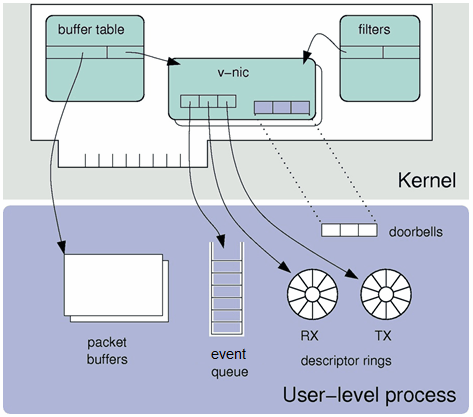
\includegraphics[width=\textwidth,height=\textheight/2,keepaspectratio=true]{efvi_vnic.png}
\doxyfigcaption{Virtual Interface Components}
\end{DoxyImage}


A virtual interface includes the following components\+:
\begin{DoxyItemize}
\item an \mbox{\hyperlink{concepts_event_queue}{Event queue}}
\item a \mbox{\hyperlink{concepts_tx_ring}{Transmit descriptor ring}}
\item a \mbox{\hyperlink{concepts_rx_ring}{Receive descriptor ring}}.
\end{DoxyItemize}

A virtual interface can be allocated one of each of these components, but if the event queue is omitted an alternative virtual interface that has an event queue must be specified.

A virtual interface also has a few hardware resources\+:
\begin{DoxyItemize}
\item a doorbell register to inform the card that new RX buffers are available for it to use
\item a doorbell register to inform the card that new TX buffers are ready for it to send
\item some timers
\item a share of an interrupt.
\end{DoxyItemize}\hypertarget{concepts_vi_sets}{}\doxysubsection{Virtual Interface Set.}\label{concepts_vi_sets}
A set of virtual interfaces can be created, to distribute load on the matching filters automatically, via {\itshape receive side scaling} (RSS).

\begin{DoxyNote}{Note}
For this to be of use, multiple filters or a wildcard filter are required. A single stream filter will have the same RSS hash for all packets. See \mbox{\hyperlink{concepts_filters}{Filters}}.
\end{DoxyNote}
\hypertarget{concepts_event_queue}{}\doxysubsection{Event queue}\label{concepts_event_queue}
An {\itshape event queue} is a channel for passing information from the network adapter to the application. It is used to notify the application of events such as the arrival of packets.\hypertarget{concepts_tx_ring}{}\doxysubsection{Transmit descriptor ring}\label{concepts_tx_ring}
The {\itshape transmit descriptor ring} is used to pass packets from the application to the adapter. Each entry in the ring is a descriptor which references a buffer containing packet data. Each packet is described by one or more descriptors.

The transmission of packets proceeds in the background, and the adapter notifies the application when they have finished via the event queue.\hypertarget{concepts_rx_ring}{}\doxysubsection{Receive descriptor ring}\label{concepts_rx_ring}
The {\itshape receive descriptor ring} is used to pass packets from the adapter to the application. The application must pre-\/allocate buffers and post them to the receive descriptor ring. Each entry in the ring is a descriptor which references a \textquotesingle{}free\textquotesingle{} buffer that the adapter can place a packet into.

When the adapter delivers a packet to an ef\+\_\+vi instance, it copies the packet data into the next available receive buffer and notifies the application via the event queue. Large packets can be scattered over multiple receive buffers.\hypertarget{concepts_pd}{}\doxysection{Protection Domain}\label{concepts_pd}
A {\itshape protection domain} identifies a separate address space for the DMA addresses passed to the adapter. It is used to protect multiple ef\+\_\+vi applications from one another, or to allow them to share resources\+:
\begin{DoxyItemize}
\item Each \mbox{\hyperlink{concepts_vi}{Virtual Interface}} is associated with one protection domain.
\item Multiple VIs can be associated with the same protection domain.
\item Each \mbox{\hyperlink{concepts_memory_region}{Memory Region}} is registered with one or more protection domains.
\item A memory region can only be used by a virtual interface that is in the same protection domain.
\item Memory regions that are registered with multiple protection domains can be used as a shared resource, for example for zero-\/copy forwarding. See also \mbox{\hyperlink{using_pb_addressing}{Packet Buffer Addressing}}.
\end{DoxyItemize}

\begin{DoxyNote}{Note}
Traditionally device drivers pass the physical addresses of memory buffers to I/O devices. This is usually acceptable because device drivers run within the privileged kernel, and so are isolated from untrusted user-\/space applications.

Applications using ef\+\_\+vi cannot in general use unprotected physical addresses, because by manipulating those addresses prior to passing them to the adapter it would be possible to access memory and devices not otherwise accessible by the application. Protection domains are used to solve this problem.
\end{DoxyNote}
\hypertarget{concepts_memory_region}{}\doxysection{Memory Region}\label{concepts_memory_region}
Any {\itshape memory region} used for transmit or receive buffers must be {\itshape registered} using the \mbox{\hyperlink{structef__memreg}{ef\+\_\+memreg}} interface. This ensures the memory region meets the requirements of ef\+\_\+vi\+:
\begin{DoxyItemize}
\item The memory is pinned, so that it can\textquotesingle{}t be swapped out to disk.
\item The memory is mapped for DMA, so that the network adapter can access it. The adapter translates the DMA addresses provided by the application to I/O addresses used on the PCIe bus.
\item The memory region is page-\/aligned, for performance.
\item The size of the memory region is a multiple of the packet buffer size, so no memory is wasted.
\end{DoxyItemize}\hypertarget{concepts_packet_buffer}{}\doxysection{Packet Buffer}\label{concepts_packet_buffer}
A {\itshape packet buffer} is a memory allocations on the host which the card will read from when sending packets, or write to when receiving packets. They are usually 2KB in size.

Packets buffers are mapped by the card in such a way that only virtual interfaces in the same protection domain can access them, unless physical addressing mode is explicitly requested. (This feature can only be granted to a group of users by the root user setting an option on the driver.)\hypertarget{concepts_jumbo}{}\doxysubsection{Jumbo Packets}\label{concepts_jumbo}
Typically, some portion of a packet buffer will be used for meta-\/data, leaving enough space for a standard sized packet. On receive, large packets will be spread out over multiple packet buffers.

When sending, multiple buffers may be used either to accommodate larger sends, or for convenience (for example\+: splitting off a standard header that is common to multiple packets).\hypertarget{concepts_descriptor}{}\doxysubsection{Packet Buffer Descriptor}\label{concepts_descriptor}
Each packet buffer is referred to by a descriptor, which contains\+:
\begin{DoxyItemize}
\item a pointer
\item an offset
\item a length.
\end{DoxyItemize}

It is those descriptors which are actually placed onto the receive and transmit descriptor rings.\hypertarget{concepts_pio}{}\doxysection{Programmed I/O}\label{concepts_pio}
The ef\+\_\+pio interface exposes a region of memory on the network adapter that can be used for low-\/latency sends. When using this interface packet data is pushed to the adapter using CPU instructions, instead of being pulled by the adapter using DMA. This reduces latency because it avoids the latency associated with a DMA read.

Applications can get even better latency by writing packet data to the adapter in advance, before the latency critical path. On the critical path the packet data can optionally be updated before being transmitted. This improves latency because it reduces the amount of data that needs to be passed to the adapter on the critical path.\hypertarget{concepts_ctpio}{}\doxysection{Cut-\/through PIO}\label{concepts_ctpio}
CTPIO (Cut-\/through PIO) improves send latency by moving packets from the PCIe bus to network port with minimal latency. It can be used in three modes\+:
\begin{DoxyEnumerate}
\item Cut-\/through\+: The frame is transmitted onto the network as it is streamed across the PCIe bus. This mode offers the best latency.
\item Store-\/and-\/forward\+: The frame is buffered on the adapter before transmitting onto the network.
\item Store-\/and-\/forward with poison disabled\+: As for (2), except that it is guaranteed that frames are never poisoned. When this mode is enabled on any VI, all VIs are placed into store-\/and-\/forward mode.
\end{DoxyEnumerate}

Due to differences in hardware architecture, CTPIO is not available on SFN8000-\/series or earlier adapters.\hypertarget{concepts_poisoning}{}\doxysubsection{Underrun, poisoning and fallback}\label{concepts_poisoning}
When using cut-\/through mode, if the frame is not streamed to the adapter at at least line rate, then the frame is likely to be poisoned. This is most likely to happen if the application thread is interrupted while writing the frame to the adapter. In the underrun case, the frame is terminated with an invalid FCS -- this is referred to as \char`\"{}poisoning\char`\"{} -- and so will be discarded by the link partner. Cut-\/through mode is currently expected to perform well only on 10G links.

CTPIO may be aborted for other reasons, including timeout while writing a frame, contention between threads using CTPIO at the same time, and the CPU writing data to the adapter in the wrong order.

In all of the above failure cases the adapter falls-\/back to sending via the traditional DMA mechanism, which incurs a latency penalty. So a valid copy of the packet is always transmitted, whether the CTPIO operation succeeds or not.

After a non-\/\+CTPIO send (including DMA fallback), the TX queue must empty before a CTPIO can again succeed.

Normally only an underrun in cut-\/through mode will result in a poisoned frame being transmitted. In rare cases it is also possible for a poisoned frame to be emitted in store-\/and-\/forward mode. If it is necessary to strictly prevent poisoned packets from reaching the network, then poisoning can be disabled globally.\hypertarget{concepts_ctpio_diagnostics}{}\doxysubsection{CTPIO diagnostics}\label{concepts_ctpio_diagnostics}
The adapter maintains counters that show whether CTPIO is being used, and any reasons for CTPIO sends failing. These can be inspected as follows\+:


\begin{DoxyCode}{0}
\DoxyCodeLine{ethtool -\/S ethX | grep ctpio}

\end{DoxyCode}


Note that some of these counters are maintained on a per-\/adapter basis, whereas others are per network port.\hypertarget{concepts_filters}{}\doxysection{Filters}\label{concepts_filters}
{\itshape Filters} select which packets are delivered to a virtual interface. Packets that are not selected are ignored and allowed to pass on to the kernel.

Each filter specifies the characteristics of packets for selection. These characteristics are typically packet header fields, including Ethernet MAC address, VLAN tags, IP addresses and port numbers.

A selected packet can be\+:
\begin{DoxyItemize}
\item Stolen\+: the packet is delivered to the virtual interface, but not to the kernel stack.
\item Replicated\+: a copy is delivered to the virtual interface, and might also be delivered to other consumers. Used for multicast packets.
\item Sniffed\+: the packet is delivered to the virtual interface, and to the kernel stack.
\end{DoxyItemize}

\begin{DoxyNote}{Note}
The set of header fields and filter modes that are available vary between adapter model and firmware variant.
\end{DoxyNote}
\hypertarget{concepts_multiple_filters}{}\doxysubsection{Multiple Filters}\label{concepts_multiple_filters}
An ef\+\_\+vi application can set multiple types of filters on the same virtual interface. Setting an invalid filter or combination of filters causes an error.\hypertarget{concepts_vlan}{}\doxysection{Virtual LANs}\label{concepts_vlan}
Ef\+\_\+vi only has limited support for {\itshape Virtual LANs} (VLANs). This is because ef\+\_\+vi operates at the Ethernet frame level, whereas VLANs are usually handled at a higher level\+:
\begin{DoxyItemize}
\item Received packets can be filtered by VLAN, but this requires a recent adapter running full feature firmware. There are also limitations on what other filters can simultaneously be used. For more details, see \mbox{\hyperlink{vi_8h_a5f8e4fb095dc588c49cfcbc064ef7810}{ef\+\_\+filter\+\_\+spec\+\_\+set\+\_\+vlan()}}.
\item Transmitted packets can have their VLAN set by adding the desired VLAN tag to the extended header. Unlike checksums, ef\+\_\+vi does not provide an offload for this.
\end{DoxyItemize}\hypertarget{concepts_tx_alternatives}{}\doxysection{TX Alternatives}\label{concepts_tx_alternatives}
{\itshape TX alternatives} is a feature available on Solarflare SFN8000 series adapters to provide multiple alternative queues for transmission, that can be used to minimize latency. Different possible responses can be pushed through the TX path on the NIC, and held in different queues ready to transmit. When it is decided which response to transmit, the appropriate alternative queue is selected, and the queued packets are sent. Because the packets are already prepared, and are held close to the wire, latency is greatly reduced. 
\chapter{Example Applications}
\label{applications}
\Hypertarget{applications}
Solarflare ef\+\_\+vi comes with a range of example applications -\/ including source code and make files. This is a quick guide to using them, both for testing ef\+\_\+vi\textquotesingle{}s effectiveness in an environment, and as starting points for developing applications.

Most of these applications have additional options to test physical addressing mode, or hardware timestamping. Run with \char`\"{}-\/-\/help\char`\"{} to check this.

\tabulinesep=1mm
\begin{longtabu}spread 0pt [c]{*{2}{|X[-1]}|}
\hline
\cellcolor{\tableheadbgcolor}\textbf{ Application   }&\cellcolor{\tableheadbgcolor}\textbf{ Description    }\\\cline{1-2}
\endfirsthead
\hline
\endfoot
\hline
\cellcolor{\tableheadbgcolor}\textbf{ Application   }&\cellcolor{\tableheadbgcolor}\textbf{ Description    }\\\cline{1-2}
\endhead
\mbox{\hyperlink{applications_eflatency}{eflatency}}   &Measure latency by pinging a simple message between two interfaces.    \\\cline{1-2}
\mbox{\hyperlink{applications_efsend}{efsend}}   &Send UDP packets on a specified interface.    \\\cline{1-2}
\mbox{\hyperlink{applications_efsink}{efsink}}   &Receive streams of packets on a single interface.    \\\cline{1-2}
\mbox{\hyperlink{applications_efforward}{efforward}}   &Forward packets between two interfaces without modification.    \\\cline{1-2}
\mbox{\hyperlink{applications_efsend_timestamping}{efsend\+\_\+timestamping}}   &Send UDP packets on a specified interface, with TX timestamping.    \\\cline{1-2}
\mbox{\hyperlink{applications_efsend_pio}{efsend\+\_\+pio}}   &Send UDP packets on a specified interface using Programmed I/O.    \\\cline{1-2}
\mbox{\hyperlink{applications_efsend_pio_warm}{efsend\+\_\+pio\+\_\+warm}}   &Send UDP packets on a specified interface using Programmed I/O with transmit warming.    \\\cline{1-2}
\mbox{\hyperlink{applications_efsink_packed}{efsink\+\_\+packed}}   &Receive streams of packets on a single interface using packed streams.    \\\cline{1-2}
\mbox{\hyperlink{applications_efforward_packed}{efforward\+\_\+packed}}   &Forward packets between two interfaces without modification using packed stream mode for receive.    \\\cline{1-2}
\mbox{\hyperlink{applications_efrss}{efrss}}   &Forward packets between two interfaces without modification, spreading the load over multiple virtual interfaces and threads.    \\\cline{1-2}
\mbox{\hyperlink{applications_efjumborx}{efjumborx}}   &Receive jumbo packets.    \\\cline{1-2}
\mbox{\hyperlink{applications_exchange}{exchange}}   &Simplified electronic trading exchange.    \\\cline{1-2}
\mbox{\hyperlink{applications_trader_onload_ds_efvi}{trader\+\_\+onload\+\_\+ds\+\_\+efvi}}   &Simplified electronic trader.    \\\cline{1-2}
\mbox{\hyperlink{applications_efrink_controller}{efrink\+\_\+controller}}   &Receive packets on a single interface into a shared memory ring.    \\\cline{1-2}
\mbox{\hyperlink{applications_efrink_consumer}{efrink\+\_\+consumer}}   &Consume packets from a shared memory ring.   \\\cline{1-2}
\end{longtabu}
\hypertarget{applications_eflatency}{}\doxysection{eflatency}\label{applications_eflatency}
The eflatency application echoes a single packet back and forth repeatedly, measuring the round-\/trip time.

This is the most useful example application for testing lowest possible latency. It is not a very good sample for building an application, because\+:
\begin{DoxyItemize}
\item it uses only one filter
\item it operates knowing that there is only ever a single packet on the wire, and so\+:
\begin{DoxyItemize}
\item does not need to refill the rings
\item does not handle multiple event types.
\end{DoxyItemize}
\end{DoxyItemize}\hypertarget{applications_eflatency_usage}{}\doxysubsection{Usage}\label{applications_eflatency_usage}
{\bfseries{Server\+:}} {\ttfamily eflatency pong {\itshape interface}}

{\bfseries{Client\+:}} {\ttfamily eflatency ping {\itshape interface}}

where\+:
\begin{DoxyItemize}
\item {\itshape interface} is the multicast interface on the server or client machine (e.\+g. {\ttfamily eth0})
\end{DoxyItemize}

There are various additional options. See the help text for details.\hypertarget{applications_efsend}{}\doxysection{efsend}\label{applications_efsend}
The efsend application sends UDP packets on a specified interface.

The application sends a UDP packet, waits for transmission of the packet to finish and then sends the next.

The number of packets sent, the size of the packet, the amount of time to wait between sends can be controlled.\hypertarget{applications_efsink}{}\doxysection{efsink}\label{applications_efsink}
The efsink application is a demonstration of capturing packets, and the flexibility of filters.

It supports all filter types that ef\+\_\+vi supports. By default it just reports the amount of data captured, but it also demonstrates simple actions upon the packet data, with the option to hexdump incoming packets.

It is a very useful jumping off point as it shows\+:
\begin{DoxyItemize}
\item creation of a virtual interface
\item creation and installation of filters
\item polling the event queue.
\end{DoxyItemize}\hypertarget{applications_efsink_usage}{}\doxysubsection{Usage}\label{applications_efsink_usage}
To receive a single multicast group\+:

efsink {\ttfamily {\itshape local interface} udp\+:$<$multicast-\/addr$>$\+:port}

To receive multiple multicast groups\+:

efsink {\ttfamily {\itshape interface} udp\+:$<$multicast-\/addr$>$\+:port udp\+:$<$multicast-\/group$>$\+:port}

To receive all multicast traffic\+:

efsink {\ttfamily {\itshape interface} multicast-\/all}

The efsink application does not send packets.\hypertarget{applications_efforward}{}\doxysection{efforward}\label{applications_efforward}
The efforward application listens for traffic on one interface and echoes it out of a second; and vice versa. It demonstrates a very simple high-\/performance bridge.

Some route configuration on the clients might be necessary to get this working, but it is a very simple example, and is very easy to start adding packet re-\/writing rules etc.

Although this is a viable starting point for a bridging application, a better option might be the Solar\+Capture API, which includes a more complete pre-\/made bridging application.\hypertarget{applications_efsend_timestamping}{}\doxysection{efsend\+\_\+timestamping}\label{applications_efsend_timestamping}
The efsend\+\_\+timestamping application sends UDP packets on a specified interface.

The application sends a UDP packet, waits for transmission of the packet to finish and then sends the next.

This application requests tx timestamping, allowing it to report the time each packet was transmitted.

The number of packets sent, the size of the packet, the amount of time to wait between sends can be controlled.\hypertarget{applications_efsend_pio}{}\doxysection{efsend\+\_\+pio}\label{applications_efsend_pio}
The efsend\+\_\+pio application sends UDP packets on a specified interface.

Packet data is copied to the NIC\textquotesingle{}s PIO buffer before being sent, which typically results in lower latency sends compared to accessing packet data stored on the host via DMA, which is the method used by the efsend sample app.

The application sends a UDP packet, waits for transmission of the packet to finish and then sends the next.

The number of packets sent, the size of the packet, the amount of time to wait between sends can be controlled.\hypertarget{applications_efsend_pio_warm}{}\doxysection{efsend\+\_\+pio\+\_\+warm}\label{applications_efsend_pio_warm}
The efsend\+\_\+pio\+\_\+warm application demonstrates PIO transmit warming.

The application sends a UDP packet using PIO each time a trigger fires. While waiting for a trigger, the application can warm the PIO transmit path to reduce latency of the subsequent send.

The effect of warming can be assessed by measuring the time from when the trigger fires to when the corresponding packet leaves the adapter.

Several parameters can be controlled including the delay between triggers, the enablement of warming and the frequency of warming while waiting for a trigger.\hypertarget{applications_efsink_packed}{}\doxysection{efsink\+\_\+packed}\label{applications_efsink_packed}
The efsink\+\_\+packed application is a variant of \mbox{\hyperlink{applications_efsink}{efsink}} that demonstrates usage of the packed-\/stream firmware.\hypertarget{applications_efforward_packed}{}\doxysection{efforward\+\_\+packed}\label{applications_efforward_packed}
The efforward\+\_\+packed application is a variant of \mbox{\hyperlink{applications_efforward}{efforward}} that demonstrates usage of the packed-\/stream firmware.\hypertarget{applications_efrss}{}\doxysection{efrss}\label{applications_efrss}
The efrss application is a variant of \mbox{\hyperlink{applications_efforward}{efforward}}. It demonstrates automatically spreading the load over multiple threads, using a vi\+\_\+set and RSS.\hypertarget{applications_efdelegated_client}{}\doxysection{efdelegated\+\_\+client}\label{applications_efdelegated_client}
The efdelegated\+\_\+client application demonstrates usage of Open\+Onload\textquotesingle{}s \char`\"{}\+Delegated Sends\char`\"{} feature. This API allows you to do delegate TCP sends for a particular socket to some other mechanism. For example, this sample uses the ef\+\_\+vi layer-\/2 API in order to get lower latency than is possible with a normal send() call.

The API essentially boils down to first retrieving the packet headers, adding your own payload to form a raw packet, sending the packet and finally telling Onload what it was you sent so it can update the internal TCP state of the socket.

This sample application allows you to compare the performance of normal sends using the kernel stack, using Open\+Onload and using ef\+\_\+vi with the delegated sends API. It establishes a TCP connection to the server process, which starts sending UDP multicast messages. The client receives these messages, and replies to a subset of them with a TCP message. The server measures the latency from the UDP send to the TCP receive.\hypertarget{applications_efjumborx}{}\doxysection{efjumborx}\label{applications_efjumborx}
The efjumborx application demonstrates receiving jumbo packets.

Various parameters can be set, including the interface, IP address and port to use. Verbose output can be enabled to view progress. The received packet can be printed as text or in hexadecimal.\hypertarget{applications_exchange}{}\doxysection{exchange}\label{applications_exchange}
The exchange application plays the role of a simplified electronic trading exchange. It is to be used in conjunction with the \mbox{\hyperlink{applications_trader_onload_ds_efvi}{trader\+\_\+onload\+\_\+ds\+\_\+efvi}} application.\hypertarget{applications_trader_onload_ds_efvi}{}\doxysection{trader\+\_\+onload\+\_\+ds\+\_\+efvi}\label{applications_trader_onload_ds_efvi}
The trader\+\_\+onload\+\_\+ds\+\_\+efvi application demonstrates various techniques to reduce latency. These techniques are often useful in electronic trading applications, and so this example takes the form of an extremely simplified electronic trading system.

The \mbox{\hyperlink{applications_exchange}{exchange}} application provides a simplified electronic trading exchange, and this application provides a simplified electronic trader.

A trader\+\_\+onload\+\_\+ds\+\_\+efvi application demonstrates similar techniques for Onload.

For full details, see the {\ttfamily README} file in the {\ttfamily tests/trade\+\_\+sim} directory.\hypertarget{applications_trader_onload_ds_efvi_usage}{}\doxysubsection{Usage}\label{applications_trader_onload_ds_efvi_usage}
For normal socket-\/based sends, run as follows\+:

{\bfseries{Server\+:}} {\ttfamily onload -\/p latency-\/best ./exchange {\itshape mcast-\/intf}}

{\bfseries{Client\+:}} {\ttfamily onload -\/p latency-\/best ./trader\+\_\+onload\+\_\+ds\+\_\+efvi {\itshape mcast-\/intf} {\itshape server}}

For \char`\"{}delegated\char`\"{} sends, run as follows\+:

{\bfseries{Server\+:}} {\ttfamily onload -\/p latency-\/best ./exchange {\itshape mcast-\/intf}}

{\bfseries{Client\+:}} {\ttfamily onload -\/p latency-\/best ./trader\+\_\+onload\+\_\+ds\+\_\+efvi -\/d {\itshape mcast-\/intf} {\itshape server}}

where\+:
\begin{DoxyItemize}
\item {\itshape mcast-\/intf} is the multicast interface on the server or client machine (e.\+g. {\ttfamily eth0})
\item {\itshape server} is the IP address of the server machine (e.\+g. {\ttfamily 192.\+168.\+0.\+10})
\end{DoxyItemize}

There are various additional options. See the help text for details.\hypertarget{applications_efrink_controller}{}\doxysection{efrink\+\_\+controller}\label{applications_efrink_controller}
The efrink\+\_\+controller application receives streams of packets on a single interface into a shared memory ring. This can be read by multiple consumers, such as \mbox{\hyperlink{applications_efrink_consumer}{efrink\+\_\+consumer}}.

This is an advanced technique which has the potential to provide a more efficient way to receive data when multiple consumer processes want to receive the same data stream(s) from the network.

A single controller sets up a region of shared memory, and posts chunks of this to the RX ring of the NIC. As the NIC writes packet data, it returns completion events. The controller receives these events and marks each packet buffer as complete.

One or more readers such as \mbox{\hyperlink{applications_efrink_consumer}{efrink\+\_\+consumer}} can access the shared memory to read the packets. The data is protected via a generation counter.\hypertarget{applications_efrink_consumer}{}\doxysection{efrink\+\_\+consumer}\label{applications_efrink_consumer}
The efrink\+\_\+consumer application consumes packets from a shared memory ring, that is being managed by \mbox{\hyperlink{applications_efrink_controller}{efrink\+\_\+controller}}.

Multiple copies of efrink\+\_\+consumer can run at the same time. For best performance, all processes should share the same NUMA node/cache.\hypertarget{applications_building}{}\doxysection{Building the Example Applications}\label{applications_building}
The ef\+\_\+vi example applications are built along with the Onload installation and will be present in the {\ttfamily /\+Onload-\/$<$version$>$/build/gnu\+\_\+x86\+\_\+64/tests/ef\+\_\+vi} subdirectory. In the build directory there will be {\ttfamily gnu}, {\ttfamily gnu\+\_\+x86\+\_\+64}, {\ttfamily x86\+\_\+64\+\_\+linux-\/$<$kernel version$>$} directories\+:
\begin{DoxyItemize}
\item files under the {\ttfamily gnu} directory are 32-\/bit (if these are built)
\item files under the {\ttfamily gnu\+\_\+x86\+\_\+64} directory are 64-\/bit.
\end{DoxyItemize}

Source code files for the example applications exist in the {\ttfamily /\+Onload-\/$<$version$>$/src/tests/ef\+\_\+vi} subdirectory.

After running the onload\+\_\+install command, example applications exist in the {\ttfamily /\+Onload-\/$<$version$>$/build/gnu\+\_\+x86\+\_\+64/tests/ef\+\_\+vi} subdirectory.

To rebuild the example applications you must have the {\ttfamily Onload-\/$<$version$>$/scripts} subdirectory in your path and use the following procedure\+:


\begin{DoxyCode}{0}
\DoxyCodeLine{[root@server01 Onload-\/<version>]\# cd scripts/}
\DoxyCodeLine{[root@server01 scripts]\# export PATH="{}\$PWD:\$PATH"{}}
\DoxyCodeLine{[root@server01 scripts]\# cd ../build/gnu\_x86\_64/tests/ef\_vi/}
\DoxyCodeLine{[root@server01 ef\_vi]\# make clean}
\DoxyCodeLine{[root@serverr01 ef\_vi]\# make}

\end{DoxyCode}
 
\chapter{Using ef\+\_\+vi}
\label{using}
\Hypertarget{using}
This part of the documentation gives information on using ef\+\_\+vi to write and build applications.\hypertarget{using_components}{}\doxysection{Components}\label{using_components}
All components required to build and link a user application with the Solarflare ef\+\_\+vi API are distributed with Onload. When Onload is installed all required directories/files are located under the Onload distribution directory\+:\hypertarget{using_compiling}{}\doxysection{Compiling and Linking}\label{using_compiling}
Applications or libraries using ef\+\_\+vi will need to include the header files in src/include/etherfabric/

The application will need to be linked with libciul1.\+a or libciul.\+so, which can be found under the \char`\"{}build\char`\"{} directory after running scripts/onload\+\_\+build or scripts/onload\+\_\+install.

If compiling your application against one version of Onload, and running on a system with a different version of Onload, some care is required. Onload currently preserves compatibility and provides a stable API between the ef\+\_\+vi user-\/space and the kernel drivers, so that applications compiled using an older ef\+\_\+vi library will work when run with newer drivers. Compatibility in the other direction (newer \mbox{\hyperlink{structef__vi}{ef\+\_\+vi}} libraries running with older drivers) is not guaranteed. Finally, Onload does not currently maintain compatibility between compiling against one version of the ef\+\_\+vi libraries, and then running against another.

The simplest approach is to link statically to libciul, as this ensures that the version of the library used will match the one you have compiled against. If linking dynamically, it is recommended that you keep libciul.\+so and the application binary together. onload\+\_\+install does not install libciul.\+so into system directories to avoid the installed version being used in place of the version you compiled against.

For those wishing to use ef\+\_\+vi in combination with Onload there should be no problem linking statically to libciul and dynamically to the other libraries to allow the Onload intercepts to take effect. The ef\+\_\+delegated example application does exactly this.\hypertarget{using_using_setup}{}\doxysection{Setup}\label{using_using_setup}
Applications requiring specific features can check the versions of software\+:
\begin{DoxyItemize}
\item use \mbox{\hyperlink{ef__vi_8h_aadb4cde2a10513be23abfb17b414e7ff}{ef\+\_\+vi\+\_\+version\+\_\+str()}} to get the version of ef\+\_\+vi
\item use \mbox{\hyperlink{ef__vi_8h_a5679d140bd3bb270fa1adc2085ed36a3}{ef\+\_\+vi\+\_\+driver\+\_\+interface\+\_\+str()}} to get the char driver interface required by this build of ef\+\_\+vi.
\end{DoxyItemize}

Applications can also check for specific capabilities\+:
\begin{DoxyItemize}
\item use \mbox{\hyperlink{capabilities_8h_ae139e415401ac1c57f29e20e0356bbed}{ef\+\_\+vi\+\_\+capabilities\+\_\+get()}} to get the value of a given capability
\item use \mbox{\hyperlink{capabilities_8h_a37e23905e824f75e9452cea34de4a9dd}{ef\+\_\+vi\+\_\+capabilities\+\_\+max()}} to get the number of available capabilities
\item use \mbox{\hyperlink{capabilities_8h_a3a172e16564608f36ce31d658a043bcc}{ef\+\_\+vi\+\_\+capabilities\+\_\+name()}} to get a human-\/readable string describing a given capability.
\end{DoxyItemize}

Users of ef\+\_\+vi must do the following to setup\+:
\begin{DoxyEnumerate}
\item Obtain a driver handle by calling \mbox{\hyperlink{base_8h_acb2b46854a36c5eb295878d306a274d2}{ef\+\_\+driver\+\_\+open()}}.
\item Allocate a protection domain by calling one of the following\+:
\begin{DoxyItemize}
\item \mbox{\hyperlink{pd_8h_a65e7675bc0fb9da9551c83ada8b4b995}{ef\+\_\+pd\+\_\+alloc()}}
\item \mbox{\hyperlink{pd_8h_a0fecddb71ca39ffafe3eb68f85eb2ab6}{ef\+\_\+pd\+\_\+alloc\+\_\+by\+\_\+name()}}
\item \mbox{\hyperlink{pd_8h_ad3524370759daa4ec0bb714f865867f8}{ef\+\_\+pd\+\_\+alloc\+\_\+with\+\_\+vport()}}.
\end{DoxyItemize}
\item Allocate a virtual interface (VI), encapsulated by the type \mbox{\hyperlink{structef__vi}{ef\+\_\+vi}}, by calling \mbox{\hyperlink{vi_8h_a66124c16b919445b44e2bcba50dbc344}{ef\+\_\+vi\+\_\+alloc\+\_\+from\+\_\+pd()}}.
\end{DoxyEnumerate}


\begin{DoxyCode}{0}
\DoxyCodeLine{\textcolor{comment}{/* Allocate a protection domain */}}
\DoxyCodeLine{\textcolor{keywordtype}{int} \mbox{\hyperlink{pd_8h_a65e7675bc0fb9da9551c83ada8b4b995}{ef\_pd\_alloc}}(\mbox{\hyperlink{structef__pd}{ef\_pd}} *pd,}
\DoxyCodeLine{                \mbox{\hyperlink{base_8h_afcca014c719554b834e89f0c30e87561}{ef\_driver\_handle}} pd\_dh,}
\DoxyCodeLine{                \textcolor{keywordtype}{int} ifindex,}
\DoxyCodeLine{                \textcolor{keyword}{enum} \mbox{\hyperlink{pd_8h_a09263cdade29abed15a6775debbf27d9}{ef\_pd\_flags}} flags);}
\DoxyCodeLine{}
\DoxyCodeLine{\textcolor{keywordtype}{int} \mbox{\hyperlink{pd_8h_a0fecddb71ca39ffafe3eb68f85eb2ab6}{ef\_pd\_alloc\_by\_name}}(\mbox{\hyperlink{structef__pd}{ef\_pd}} *pd,}
\DoxyCodeLine{                        \mbox{\hyperlink{base_8h_afcca014c719554b834e89f0c30e87561}{ef\_driver\_handle}} pd\_dh,}
\DoxyCodeLine{                        \textcolor{keyword}{const} \textcolor{keywordtype}{char}* cluster\_or\_intf\_name,}
\DoxyCodeLine{                        \textcolor{keyword}{enum} \mbox{\hyperlink{pd_8h_a09263cdade29abed15a6775debbf27d9}{ef\_pd\_flags}} flags);}
\DoxyCodeLine{}
\DoxyCodeLine{\textcolor{comment}{/* Get the interface for a protection domain. */}}
\DoxyCodeLine{\textcolor{keyword}{const} \textcolor{keywordtype}{char}* \mbox{\hyperlink{pd_8h_a4e9fe7517bfbc61c291e35a6174ea1ef}{ef\_pd\_interface\_name}}(\mbox{\hyperlink{structef__pd}{ef\_pd}} *pd);}

\end{DoxyCode}
 {\bfseries{Figure\+: Create a Protection Domain}}


\begin{DoxyCode}{0}
\DoxyCodeLine{\textcolor{comment}{/* Allocate a virtual interface */}}
\DoxyCodeLine{\textcolor{keywordtype}{int} \mbox{\hyperlink{vi_8h_a66124c16b919445b44e2bcba50dbc344}{ef\_vi\_alloc\_from\_pd}}(\mbox{\hyperlink{structef__vi}{ef\_vi}} *vi, \mbox{\hyperlink{base_8h_afcca014c719554b834e89f0c30e87561}{ef\_driver\_handle}} vi\_dh,}
\DoxyCodeLine{                        \mbox{\hyperlink{structef__pd}{ef\_pd}} *pd, \mbox{\hyperlink{base_8h_afcca014c719554b834e89f0c30e87561}{ef\_driver\_handle}} pd\_dh,}
\DoxyCodeLine{                        \textcolor{keywordtype}{int} eventq\_cap, \textcolor{keywordtype}{int} rxq\_cap, \textcolor{keywordtype}{int} txq\_cap,}
\DoxyCodeLine{                        \mbox{\hyperlink{structef__vi}{ef\_vi}} *opt\_evq, \mbox{\hyperlink{base_8h_afcca014c719554b834e89f0c30e87561}{ef\_driver\_handle}} opt\_evq\_dh,}
\DoxyCodeLine{                        \textcolor{keyword}{enum} \mbox{\hyperlink{ef__vi_8h_ae6c52ae7258f201cdea370fbcf697772}{ef\_vi\_flags}} flags));}

\end{DoxyCode}
 {\bfseries{Figure\+: Allocate a Virtual Interface}}\hypertarget{using_using_vi_sets}{}\doxysubsection{Using Virtual Interface Sets.}\label{using_using_vi_sets}
A virtual interface set can be used instead of a single virtual interface, to distribute load using RSS. Functionality is almost the same as working with a single virtual interface\+:
\begin{DoxyItemize}
\item To allocate the virtual interfaces\+:
\begin{DoxyItemize}
\item use \mbox{\hyperlink{vi_8h_a341b60d550339b63abf0ad8b79828cec}{ef\+\_\+vi\+\_\+set\+\_\+alloc\+\_\+from\+\_\+pd()}} to allocate the set
\item then use \mbox{\hyperlink{vi_8h_a555084325f97dc1fe99f11295f3f1f8e}{ef\+\_\+vi\+\_\+alloc\+\_\+from\+\_\+set()}} to allocate each virtual interface in the set
\end{DoxyItemize}
\item To add a filter\+:
\begin{DoxyItemize}
\item use \mbox{\hyperlink{vi_8h_a89aa0805536fccbaf79c2120c316ff65}{ef\+\_\+vi\+\_\+set\+\_\+filter\+\_\+add()}} to add the filter onto the set, rather than adding it to each virtual interface individually (which would cause replication on a 7000-\/series NIC).
\end{DoxyItemize}
\end{DoxyItemize}

The \mbox{\hyperlink{applications_efrss}{efrss}} sample gives an example of usage.\hypertarget{using_using_buffers}{}\doxysection{Creating packet buffers}\label{using_using_buffers}
Memory used for packet buffers is allocated using standard functions such as posix\+\_\+memalign(). A packet buffer should be at least as large as the value returned from \mbox{\hyperlink{ef__vi_8h_a246e386f77279d65149236a1a6265661}{ef\+\_\+vi\+\_\+receive\+\_\+buffer\+\_\+len()}}.

The packet buffers must be pinned so that they cannot be paged, and they must be registered for DMA with the network adapter. These requirements are enforced by calling \mbox{\hyperlink{memreg_8h_ad802d1d7c6487fbeeff8ed682caf71c8}{ef\+\_\+memreg\+\_\+alloc()}} to register the allocated memory for use with ef\+\_\+vi.

The type {\ttfamily \mbox{\hyperlink{structef__iovec}{ef\+\_\+iovec}}} encapsulates a set of buffers. The adapter uses a special address space to identify locations in these buffers, and such addresses are designated by the type {\ttfamily ef\+\_\+addr}.


\begin{DoxyCode}{0}
\DoxyCodeLine{\textcolor{comment}{/* Allocate a memory region */}}
\DoxyCodeLine{\textcolor{keywordtype}{int} \mbox{\hyperlink{memreg_8h_ad802d1d7c6487fbeeff8ed682caf71c8}{ef\_memreg\_alloc}}(\mbox{\hyperlink{structef__memreg}{ef\_memreg}}* mr, \mbox{\hyperlink{base_8h_afcca014c719554b834e89f0c30e87561}{ef\_driver\_handle}} mr\_dh,}
\DoxyCodeLine{                    \mbox{\hyperlink{structef__pd}{ef\_pd}}* pd, \mbox{\hyperlink{base_8h_afcca014c719554b834e89f0c30e87561}{ef\_driver\_handle}} pd\_dh,}
\DoxyCodeLine{                    \textcolor{keywordtype}{void}* p\_mem, \textcolor{keywordtype}{int} len\_bytes);}

\end{DoxyCode}
 {\bfseries{Figure\+: Allocate a Memory Region}}

To improve performance, registered memory regions for packet buffers should be aligned on (minimum) 4KB boundaries for regular pages or 2MB boundaries when using huge pages, and should be contiguous.\hypertarget{using_buffer_tables}{}\doxysubsection{Buffer Tables}\label{using_buffer_tables}
The memory for packet buffers is mapped using a buffer table. Implementation of this can differ, but typically\+:


\begin{DoxyItemize}
\item The buffer table is allocated from memory that is also used for other things, so can vary in size
\item Entries in this table are split into sets of 32 entries
\item In the default configuration there are typically 1926 sets available, giving a maximum of 61632 entries
\item Each entry maps a chunk of naturally-\/aligned contiguous memory\+:
\begin{DoxyItemize}
\item 4KB on earlier NICs
\item 4KB, 64KB, 1MB or 4MB on 7000-\/series and later NICs
\end{DoxyItemize}
\item Each packet buffer consumes 2KB.
\end{DoxyItemize}

The total number of packet buffers available might be fewer than expected from the above\+:


\begin{DoxyItemize}
\item Some sets of entries might not be fully utilized.

In particular, the entries in a set must have the same owner ID, and so where there are multiple owner IDs, there will be unused holes in the table.
\item Setting up virtual interfaces can consume buffer table resources.

On 5000-\/ and 6000-\/series NICs, every page of host memory that is allocated to back a TX queue, RX queue or event queue uses a buffer table entry to map it. So a few hundred virtual interfaces will consume a lot of entries, especially if they are set up with large event queues.
\item The descriptor cache can reduce buffer table resources.

On 7000-\/series and later NICs, the descriptor cache consumes memory on the NIC that is otherwise available for the buffer table.
\end{DoxyItemize}\hypertarget{using_using_transmit}{}\doxysection{Transmitting Packets}\label{using_using_transmit}
To transmit packets, the basic process is\+:


\begin{DoxyEnumerate}
\item Write the packet contents (including all headers) into one or more packet buffers.

The packet buffer memory must have been previously registered with the protection domain.
\item Post a descriptor for the filled packet buffer onto the TX descriptor ring, by calling \mbox{\hyperlink{ef__vi_8h_a17215be65f036a99857092496676de26}{ef\+\_\+vi\+\_\+transmit\+\_\+init()}} and \mbox{\hyperlink{ef__vi_8h_a7bb4aa398d5a5735491e3685d6e05912}{ef\+\_\+vi\+\_\+transmit\+\_\+push()}}, or \mbox{\hyperlink{ef__vi_8h_a62408f50ae79efed0239d0b8bde3a9d8}{ef\+\_\+vi\+\_\+transmit()}}.

A doorbell is \char`\"{}rung\char`\"{} to inform the adapter that the transmit ring is non-\/empty. If the transmit descriptor ring is empty when the doorbell is rung, \textquotesingle{}TX PUSH\textquotesingle{} is used. In \textquotesingle{}TX\+\_\+\+PUSH\textquotesingle{}, the doorbell is rung and the address of the packet buffer is written in one shot improving latency. TX\+\_\+\+PUSH can cause ef\+\_\+vi to poll for events, to check if the transmit descriptor ring is empty, before sending which can lead to a latency versus throughput trade off in some scenarios.
\item Poll the event queue to find out when the transmission is complete.

See \mbox{\hyperlink{using_using_events}{Handling Events}}.

When transmitting, polling the event queue is less critical; but does still need to be done. The events of interest are {\ttfamily EF\+\_\+\+EVENT\+\_\+\+TYPE\+\_\+\+TX} or {\ttfamily EF\+\_\+\+EVENT\+\_\+\+TYPE\+\_\+\+TX\+\_\+\+WITH\+\_\+\+TIMESTAMP} telling you that a transmit completed, and {\ttfamily EF\+\_\+\+EVENT\+\_\+\+TYPE\+\_\+\+TX\+\_\+\+ERROR} telling you that a transmit failed. \mbox{\hyperlink{ef__vi_8h_aa6e256d0f1bc3c61ac6ca7aca8f96008}{EF\+\_\+\+EVENT\+\_\+\+TX\+\_\+\+Q\+\_\+\+ID()}} can be used to extract the id of the referenced packet, or you can just rely on the fact that ef\+\_\+vi always transmits packets in the order they are submitted.
\item Handle the resulting event.

Reclaim the packet buffer for re-\/use.
\end{DoxyEnumerate}


\begin{DoxyCode}{0}
\DoxyCodeLine{\textcolor{comment}{// construct packet with proper headers}}
\DoxyCodeLine{}
\DoxyCodeLine{\textcolor{comment}{// Post on the transmit ring}}
\DoxyCodeLine{\mbox{\hyperlink{ef__vi_8h_a17215be65f036a99857092496676de26}{ef\_vi\_transmit\_init}}(\&vi, addr, len, \textcolor{keywordtype}{id});}
\DoxyCodeLine{\textcolor{comment}{// Ring doorbell}}
\DoxyCodeLine{\mbox{\hyperlink{ef__vi_8h_a7bb4aa398d5a5735491e3685d6e05912}{ef\_vi\_transmit\_push}}(\&vi);}

\end{DoxyCode}
 {\bfseries{Figure\+: Transmit Packets}}\hypertarget{using_using_tx_jumbo}{}\doxysubsection{Transmitting Jumbo Frames}\label{using_using_tx_jumbo}
Packets of a size smaller than the interface MTU but larger than the packet buffer size must be sent from multiple buffers as jumbo packets. A single {\ttfamily EF\+\_\+\+EVENT\+\_\+\+TYPE\+\_\+\+TX} (or {\ttfamily EF\+\_\+\+EVENT\+\_\+\+TYPE\+\_\+\+TX\+\_\+\+ERROR}) event is raised for the entire transmit\+:


\begin{DoxyItemize}
\item Use \mbox{\hyperlink{ef__vi_8h_a10b8bcbc62dab623cd94db5aaf6ddbf0}{ef\+\_\+vi\+\_\+transmitv()}} to chain together multiple segments with a higher total length.
\item MTU is not enforced. If the transmit is to remain within MTU, the application must check and enforce this.
\item The segments must at least split along natural (4k packet) boundaries, but smaller segments can be used if desired..
\end{DoxyItemize}\hypertarget{using_using_pio}{}\doxysubsection{Programmed I/O}\label{using_using_pio}
Programmed IO is usable only on 7000-\/series cards, not on the older cards. It allows for faster transmit, especially of small packets, but the hardware resources available for it are limited.

For this reason, a PIO buffer must be explicitly allocated and associated with a virtual interface before use, by calling \mbox{\hyperlink{pio_8h_aa51c1c3a2c2c6b0c8644b1fa07458a19}{ef\+\_\+pio\+\_\+link\+\_\+vi()}}.

Data is copied into the PIO buffer with \mbox{\hyperlink{pio_8h_a1966f51d747aea4416d1a20890bb9fb4}{ef\+\_\+pio\+\_\+memcpy()}}.

When the PIO buffer is no longer required it should be unlinked by calling \mbox{\hyperlink{pio_8h_a84806b695423f76bbcc421261547b184}{ef\+\_\+pio\+\_\+unlink\+\_\+vi()}}, and then freed by calling \mbox{\hyperlink{pio_8h_acb13345a50dd777eb4f4e9a99a0e2558}{ef\+\_\+pio\+\_\+free()}}.\hypertarget{using_using_ctpio}{}\doxysubsection{Cut-\/through PIO}\label{using_using_ctpio}
A complete example showing the use of CTPIO with ef\+\_\+vi is given in {\ttfamily Onload-\/$<$version$>$/src/tests/rtt/rtt\+\_\+efvi.c}.

\begin{DoxyNote}{Note}
CTPIO bypasses the main adapter datapath, and as a result does not support checksum offload. Frames sent with CTPIO are placed on the wire without modification, so checksum fields must be completed in software before sending.
\end{DoxyNote}
Here is the sequence of steps needed\+:


\begin{DoxyEnumerate}
\item When allocating a VI (\mbox{\hyperlink{vi_8h_a66124c16b919445b44e2bcba50dbc344}{ef\+\_\+vi\+\_\+alloc\+\_\+from\+\_\+pd()}}) set the EF\+\_\+\+VI\+\_\+\+TX\+\_\+\+CTPIO flag.
\item To initiate a send, form a complete Ethernet frame (including L3/\+L4 checksums, but excluding FCS) in host memory. Initiate the send with \mbox{\hyperlink{ef__vi_8h_af1510ffff8d06a509fb23d9f0bb8f35f}{ef\+\_\+vi\+\_\+transmit\+\_\+ctpio()}} or \mbox{\hyperlink{ef__vi_8h_aca0074ba563465d5effcfc6d54b1bba2}{ef\+\_\+vi\+\_\+transmitv\+\_\+ctpio()}}.
\item Post a fall-\/back descriptor using \mbox{\hyperlink{ef__vi_8h_ab822e083cda691e17b6677629cddaf19}{ef\+\_\+vi\+\_\+transmit\+\_\+ctpio\+\_\+fallback()}} or \mbox{\hyperlink{ef__vi_8h_a77c3b1b7a28206c81ae6f67cee7662f9}{ef\+\_\+vi\+\_\+transmitv\+\_\+ctpio\+\_\+fallback()}}. These calls are used just like the standard DMA send calls (\mbox{\hyperlink{ef__vi_8h_a62408f50ae79efed0239d0b8bde3a9d8}{ef\+\_\+vi\+\_\+transmit()}} etc.), and so must be provided with a copy of the frame in registered memory.
\end{DoxyEnumerate}

The posting of a fall-\/back descriptor is not on the latency critical path, provided the CTPIO operation succeeds. However, it must be posted before posting any further sends on the same VI.\hypertarget{using_using_tx_alternatives}{}\doxysubsection{TX Alternatives}\label{using_using_tx_alternatives}
TX alternatives is a features available on Solarflare SFN8000 series adapters. To use TX alternatives for a given virtual interface, you must set the EF\+\_\+\+VI\+\_\+\+TX\+\_\+\+ALT flag when you allocate the virtual interface. You must then allocate a set of TX alternatives for the virtual interface by calling \mbox{\hyperlink{vi_8h_aca91a5b7b6569d14c434ca242ecf3af9}{ef\+\_\+vi\+\_\+transmit\+\_\+alt\+\_\+alloc()}}.


\begin{DoxyCode}{0}
\DoxyCodeLine{\textcolor{keywordtype}{int} \mbox{\hyperlink{vi_8h_aca91a5b7b6569d14c434ca242ecf3af9}{ef\_vi\_transmit\_alt\_alloc}}(\textcolor{keyword}{struct} \mbox{\hyperlink{structef__vi}{ef\_vi}}* vi, \mbox{\hyperlink{base_8h_afcca014c719554b834e89f0c30e87561}{ef\_driver\_handle}} vi\_dh,}
\DoxyCodeLine{                             \textcolor{keywordtype}{int} num\_alts, \textcolor{keywordtype}{int} buf\_space);}

\end{DoxyCode}


The number of virtual interfaces that can use TX alternatives simultaneously is limited, and varies by adapter and port mode. Typical limitations are as follows\+:
\begin{DoxyItemize}
\item SFN8522, 2x10\+Gb\+: at least 6 virtual interfaces can use TX alternatives
\item SFN8542, 2x40\+Gb\+: at least 6 virtual interfaces can use TX alternatives
\item SFN8542, 1x40\+Gb + 2x10\+Gb\+: at least 3 virtual interfaces can use TX alternatives
\item SFN8542, 4x10\+Gb\+: TX alternatives are {\itshape not} available.
\end{DoxyItemize}

This creates a set of TX alternatives. The TX alternatives remain allocated until the virtual interface is freed. They are given sequential IDs, from 0 upwards.

You can get the number of TX alternatives in a set by calling \mbox{\hyperlink{ef__vi_8h_a068a248d1af10a594c10878fe029ff53}{ef\+\_\+vi\+\_\+transmit\+\_\+alt\+\_\+num\+\_\+ids()}}.


\begin{DoxyCode}{0}
\DoxyCodeLine{\textcolor{keywordtype}{unsigned} \mbox{\hyperlink{ef__vi_8h_a068a248d1af10a594c10878fe029ff53}{ef\_vi\_transmit\_alt\_num\_ids}}(\mbox{\hyperlink{structef__vi}{ef\_vi}}* vi);}

\end{DoxyCode}


You can then buffer responses on the different TX alternatives, choose which to transmit, and discard any that are no longer required\+:


\begin{DoxyItemize}
\item All TX alternatives are initially in the STOP state, and any packets sent to them are buffered.
\item To send packets to a particular TX alternative, select the TX alternative by calling \mbox{\hyperlink{ef__vi_8h_add2a128213fafba3ebb74d137ab36178}{ef\+\_\+vi\+\_\+transmit\+\_\+alt\+\_\+select()}}, and then send the packets to the virtual interface using normal send calls such as \mbox{\hyperlink{ef__vi_8h_a62408f50ae79efed0239d0b8bde3a9d8}{ef\+\_\+vi\+\_\+transmit()}}.
\item To transmit the packets that are buffered on a TX alternative, call \mbox{\hyperlink{ef__vi_8h_a70e8d8c2fa4927392174223bcdd2cc31}{ef\+\_\+vi\+\_\+transmit\+\_\+alt\+\_\+go()}}.

This transitions the TX alternative to the GO state. While the TX alternative remains in this state, any further packets sent to it are transmitted immediately.
\item To transition the TX alternative back to the STOP state, call \mbox{\hyperlink{ef__vi_8h_a51050ee6dc126b1326c6d5775808e639}{ef\+\_\+vi\+\_\+transmit\+\_\+alt\+\_\+stop()}}.
\item To discard the packets buffered on a TX alternative, transition it to the DISCARD state by calling \mbox{\hyperlink{ef__vi_8h_ac273e4b11c2b98664cf7363574eb5f70}{ef\+\_\+vi\+\_\+transmit\+\_\+alt\+\_\+discard()}}.
\end{DoxyItemize}


\begin{DoxyCode}{0}
\DoxyCodeLine{\textcolor{keywordtype}{int} \mbox{\hyperlink{ef__vi_8h_add2a128213fafba3ebb74d137ab36178}{ef\_vi\_transmit\_alt\_select}}(\textcolor{keyword}{struct} \mbox{\hyperlink{structef__vi}{ef\_vi}}* vi, \textcolor{keywordtype}{unsigned} alt\_id);}
\DoxyCodeLine{}
\DoxyCodeLine{\textcolor{keywordtype}{int} \mbox{\hyperlink{ef__vi_8h_a51050ee6dc126b1326c6d5775808e639}{ef\_vi\_transmit\_alt\_stop}}(\textcolor{keyword}{struct} \mbox{\hyperlink{structef__vi}{ef\_vi}}* vi, \textcolor{keywordtype}{unsigned} alt\_id);}
\DoxyCodeLine{}
\DoxyCodeLine{\textcolor{keywordtype}{int} \mbox{\hyperlink{ef__vi_8h_a70e8d8c2fa4927392174223bcdd2cc31}{ef\_vi\_transmit\_alt\_go}}(\textcolor{keyword}{struct} \mbox{\hyperlink{structef__vi}{ef\_vi}}* vi, \textcolor{keywordtype}{unsigned} alt\_id);}
\DoxyCodeLine{}
\DoxyCodeLine{\textcolor{keywordtype}{int} \mbox{\hyperlink{ef__vi_8h_ac273e4b11c2b98664cf7363574eb5f70}{ef\_vi\_transmit\_alt\_discard}}(\textcolor{keyword}{struct} \mbox{\hyperlink{structef__vi}{ef\_vi}}* vi, \textcolor{keywordtype}{unsigned} alt\_id);}

\end{DoxyCode}


As packets are transmitted or discarded, events of type EF\+\_\+\+EVENT\+\_\+\+TYPE\+\_\+\+TX\+\_\+\+ALT are returned to your application. Your application should normally wait until all packets have been processed before transitioning to a different state.

Calls are available to calculate the buffer usage\+:


\begin{DoxyItemize}
\item To query the amount of user-\/visible buffering that will be available, call \mbox{\hyperlink{vi_8h_a16b8fed8c7b4af2cbcdc559d8ac28572}{ef\+\_\+vi\+\_\+transmit\+\_\+alt\+\_\+query\+\_\+buffering()}}
\item To query the per-\/packet overheads, call \mbox{\hyperlink{ef__vi_8h_a89b67172b16e9baa8ea4a638c17329a9}{ef\+\_\+vi\+\_\+transmit\+\_\+alt\+\_\+query\+\_\+overhead()}}.
\item To calculate a packet\textquotesingle{}s buffer usage, pass the per-\/packet overheads and the packet length to \mbox{\hyperlink{ef__vi_8h_a18add9a422a88041e5349700a54d457e}{ef\+\_\+vi\+\_\+transmit\+\_\+alt\+\_\+usage()}}.
\end{DoxyItemize}


\begin{DoxyCode}{0}
\DoxyCodeLine{\textcolor{keywordtype}{int} \mbox{\hyperlink{vi_8h_a16b8fed8c7b4af2cbcdc559d8ac28572}{ef\_vi\_transmit\_alt\_query\_buffering}}(\textcolor{keyword}{struct} \mbox{\hyperlink{structef__vi}{ef\_vi}}* vi, \textcolor{keywordtype}{int} ifindex,}
\DoxyCodeLine{                                       \mbox{\hyperlink{base_8h_afcca014c719554b834e89f0c30e87561}{ef\_driver\_handle}} vi\_dh, \textcolor{keywordtype}{int} n\_alts);}
\DoxyCodeLine{}
\DoxyCodeLine{\textcolor{keywordtype}{int}}
\DoxyCodeLine{\mbox{\hyperlink{ef__vi_8h_a89b67172b16e9baa8ea4a638c17329a9}{ef\_vi\_transmit\_alt\_query\_overhead}}(\mbox{\hyperlink{structef__vi}{ef\_vi}}* vi,}
\DoxyCodeLine{                                  \textcolor{keyword}{struct} \mbox{\hyperlink{structef__vi__transmit__alt__overhead}{ef\_vi\_transmit\_alt\_overhead}}* params);}
\DoxyCodeLine{}
\DoxyCodeLine{uint32\_t}
\DoxyCodeLine{\mbox{\hyperlink{ef__vi_8h_a18add9a422a88041e5349700a54d457e}{ef\_vi\_transmit\_alt\_usage}}(\textcolor{keyword}{const} \textcolor{keyword}{struct} \mbox{\hyperlink{structef__vi__transmit__alt__overhead}{ef\_vi\_transmit\_alt\_overhead}}* params,}
\DoxyCodeLine{                         uint32\_t pkt\_len);}

\end{DoxyCode}
\hypertarget{using_using_events}{}\doxysection{Handling Events}\label{using_using_events}
The event queue is a channel from the adapter to software which notifies software when packets arrive from the network, and when transmits complete (so that the buffers can be freed or reused). Application threads retrieve these events in one of the following ways\+:
\begin{DoxyItemize}
\item A thread can busy-\/wait for an event notification by calling \mbox{\hyperlink{ef__vi_8h_ab340116b526f45dd378fe279f0c05a48}{ef\+\_\+eventq\+\_\+poll()}} repeatedly in a tight loop. This gives the lowest latency.
\item A thread can block until event notifications arrive (or a timeout expires) by calling \mbox{\hyperlink{base_8h_a282e0ba3717d2e509cd4ebc984f62461}{ef\+\_\+eventq\+\_\+wait()}}. This frees the CPU for other usage.
\end{DoxyItemize}

The batch size for polling must be at least EF\+\_\+\+VI\+\_\+\+EVENT\+\_\+\+POLL\+\_\+\+MIN\+\_\+\+EVS. It should be greater than the batch size for refilling to detect when the receive descriptor ring is going empty.

When timestamping is enabled, a number of timestamps per second are added to the event queue, even when no packets are being received. It is important that the application regularly polls the VI event queue, to avoid an event queue overflow (EF\+\_\+\+EVENT\+\_\+\+TYPE\+\_\+\+OFLOW) which can result in an undetermined state for the VI.\hypertarget{using_fd_blocking}{}\doxysubsection{Blocking on a file descriptor}\label{using_fd_blocking}
Ef\+\_\+vi supports integration with other types of I/O via the select, poll and epoll interfaces. Each virtual interface is associated with a file descriptor. The ef\+\_\+vi layer supports blocking on a file descriptor until it has events ready, when it becomes readable. This feature provides the functionality that is already provided by \mbox{\hyperlink{base_8h_a282e0ba3717d2e509cd4ebc984f62461}{ef\+\_\+eventq\+\_\+wait()}} with the added benefit that as you are blocking on a file descriptor, you can block for events on a virtual interface along with other file descriptors at the same time.

The file descriptor to use for blocking is the driver handle that was used to allocate the virtual interface.

Before you can block on the file descriptor, you need to prime interrupts on the virtual interface. This is done by calling \mbox{\hyperlink{vi_8h_a7940e2ef8c2df90ce777e6db1556e19a}{ef\+\_\+vi\+\_\+prime()}}.


\begin{DoxyCode}{0}
\DoxyCodeLine{\textcolor{keywordtype}{int} \mbox{\hyperlink{vi_8h_a7940e2ef8c2df90ce777e6db1556e19a}{ef\_vi\_prime}}(\mbox{\hyperlink{structef__vi}{ef\_vi}}* vi, \mbox{\hyperlink{base_8h_afcca014c719554b834e89f0c30e87561}{ef\_driver\_handle}} dh,}
\DoxyCodeLine{                \textcolor{keywordtype}{unsigned} current\_ptr);}

\end{DoxyCode}


When this function is called, you must tell it how many events you\textquotesingle{}ve read from the eventq which can be retrieved by using \mbox{\hyperlink{ef__vi_8h_a4729338fad56b630f44ae1b2515dfd69}{ef\+\_\+eventq\+\_\+current()}}. Then you can simply block on the file descriptor becoming readable by using select(), poll(), epoll(), etc. When the file descriptor is returned as readable, you can then get the associated events by polling the eventq in the normal way. Note that at this point, you must call \mbox{\hyperlink{vi_8h_a7940e2ef8c2df90ce777e6db1556e19a}{ef\+\_\+vi\+\_\+prime()}} again (with the current value from \mbox{\hyperlink{ef__vi_8h_a4729338fad56b630f44ae1b2515dfd69}{ef\+\_\+eventq\+\_\+current()}}) before blocking on the file descriptor again.

The \mbox{\hyperlink{applications_efsink}{efsink}} example code offers a simple example.\hypertarget{using_using_receive}{}\doxysection{Receiving packets}\label{using_using_receive}
To receive packets, the basic process is\+:


\begin{DoxyEnumerate}
\item Post descriptors for empty packet buffers onto the RX descriptor ring, by calling \mbox{\hyperlink{ef__vi_8h_a9e1fbd2c66475fde3aa1b7df19841ef9}{ef\+\_\+vi\+\_\+receive\+\_\+init()}} and \mbox{\hyperlink{ef__vi_8h_abcd5dc1be7ff1e9f9a4a84df86305099}{ef\+\_\+vi\+\_\+receive\+\_\+push()}}, or \mbox{\hyperlink{ef__vi_8h_aa5ffb14e493b05738eb74fc44ca2be71}{ef\+\_\+vi\+\_\+receive\+\_\+post()}}.

Receive descriptors should be posted in multiples of 8. When an application pushes 10 descriptors, ef\+\_\+vi will push 8 and ef\+\_\+vi will ignore descriptor batch sizes $<$ 8. Users should beware that if the ring is empty and the application pushes $<$ 8 descriptors before blocking on the event queue, the application will remain blocked as there are no descriptors available to receive packets so nothing gets posted to the event queue.

Posting descriptors should ideally be done in batches, by a thread that is not on the critical path. A small batch size means that the ring is kept more full, but a large batch size is more efficient. A size of 8, 16 or 32 is probably the best compromise.
\item Poll the event queue to see that they are now filled.

See \mbox{\hyperlink{using_using_events}{Handling Events}}.

Packets are written into the buffers in FIFO order.
\item Handle the resulting event and the incoming packet.

Since the adapter is cut-\/through, errors in receiving packets like multicast mismatch, CRC errors, etc. are delivered along with the packet. The software must detect these errors and recycle the associated packet buffers.
\end{DoxyEnumerate}\hypertarget{using_packet_data}{}\doxysubsection{Finding the Packet Data}\label{using_packet_data}
Use the queue ID to find the packet and its buffer. The diagram below shows the layout of the buffer, and the functions and macros for accessing it\+:

  
\begin{DoxyImage}
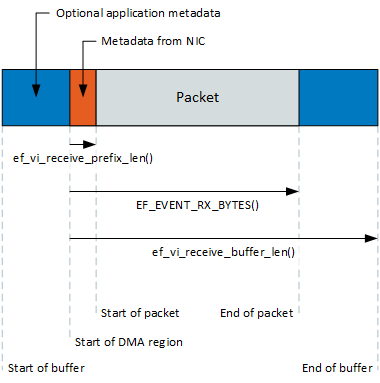
\includegraphics[width=\textwidth,height=\textheight/2,keepaspectratio=true]{packet_buffers_layout.png}
\doxyfigcaption{Layout and functions for a packet buffer}
\end{DoxyImage}



\begin{DoxyItemize}
\item Use \mbox{\hyperlink{ef__vi_8h_a7a58c5a2ac989e1b24f33f5d7bb7f348}{ef\+\_\+vi\+\_\+receive\+\_\+prefix\+\_\+len()}} to find the offset for the packet data. (Remember that this includes the headers, as ef\+\_\+vi does not do any protocol handling.)
\item \mbox{\hyperlink{ef__vi_8h_abc676af3c8675d8bf305f6313252c55f}{EF\+\_\+\+EVENT\+\_\+\+RX\+\_\+\+BYTES()}} gives the number of bytes received.
\item \mbox{\hyperlink{ef__vi_8h_a3c1a5ccee11cafca42a09646581b8fcb}{ef\+\_\+vi\+\_\+receive\+\_\+query\+\_\+layout()}} gives more information.
\end{DoxyItemize}

Packets that are smaller than the packet buffer size are delivered one per packet buffer. An event is raised for each packet buffer that is filled\+:

  
\begin{DoxyImage}
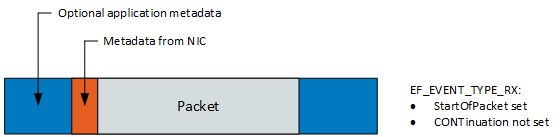
\includegraphics[width=\textwidth,height=\textheight/2,keepaspectratio=true]{packet_buffers_non-jumbo.png}
\doxyfigcaption{A single (non-\/jumbo) packet}
\end{DoxyImage}
\hypertarget{using_using_rx_jumbo}{}\doxysubsection{Receiving Jumbo Packets}\label{using_using_rx_jumbo}
Packets of a size smaller than the interface MTU but larger than the packet buffer size are delivered in multiple buffers as jumbo packets. An event is raised for each packet buffer that is filled. For example, this is a packet that requires two buffers\+:

  
\begin{DoxyImage}
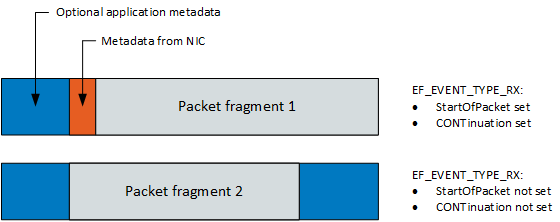
\includegraphics[width=\textwidth,height=\textheight/2,keepaspectratio=true]{packet_buffers_jumbo-2.png}
\doxyfigcaption{A 2-\/buffer jumbo packet}
\end{DoxyImage}


and this is a larger packet that requires {\itshape N} buffers\+:

  
\begin{DoxyImage}
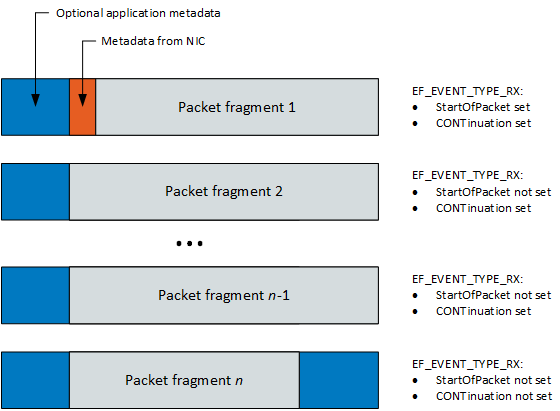
\includegraphics[width=\textwidth,height=\textheight/2,keepaspectratio=true]{packet_buffers_jumbo-n.png}
\doxyfigcaption{An N-\/buffer jumbo packet}
\end{DoxyImage}



\begin{DoxyItemize}
\item The \mbox{\hyperlink{ef__vi_8h_a2c9f892479de9126f6a731ff5f8d65be}{EF\+\_\+\+EVENT\+\_\+\+RX\+\_\+\+CONT()}} macro can be used to check if this is not the last part of the packet, and that the next receive (on this RX descriptor ring) should also be examined as being part of this jumbo frame.
\item The \mbox{\hyperlink{ef__vi_8h_abc676af3c8675d8bf305f6313252c55f}{EF\+\_\+\+EVENT\+\_\+\+RX\+\_\+\+BYTES()}} macro gets the number of bytes of the packet that have been received. This is a cumulative total, so the value for the last part of the frame is the total packet length.
\item If {\ttfamily EF\+\_\+\+EVENT\+\_\+\+RX\+\_\+\+DISCARD\+\_\+\+TRUNC} is set, this indicates that the packet buffer has been dropped, and so the jumbo packet has been truncated. But there might still be more parts of the jumbo packet that arrive after the drop. All packet buffers should be discarded until one is received with {\ttfamily EF\+\_\+\+EVENT\+\_\+\+RX\+\_\+\+SOP} set, marking the start of a new packet.
\end{DoxyItemize}\hypertarget{using_using_rx_event_merging}{}\doxysubsection{RX Event Merging}\label{using_using_rx_event_merging}
RX event merging can merge multiple events into a single {\ttfamily EF\+\_\+\+EVENT\+\_\+\+TYPE\+\_\+\+RX\+\_\+\+MULTI} event\+:


\begin{DoxyItemize}
\item There can potentially be multiple packets per event.
\item Events can only be merged to a single {\ttfamily EF\+\_\+\+EVENT\+\_\+\+TYPE\+\_\+\+RX\+\_\+\+MULTI} event when their flags are the same.
\item When an {\ttfamily EF\+\_\+\+EVENT\+\_\+\+TYPE\+\_\+\+RX\+\_\+\+MULTI} event occurs, \mbox{\hyperlink{ef__vi_8h_a7da657579f196e3a895e4527eb958d65}{ef\+\_\+vi\+\_\+receive\+\_\+unbundle()}} must always be used to find the individual buffers.
\item When an {\ttfamily EF\+\_\+\+EVENT\+\_\+\+TYPE\+\_\+\+RX\+\_\+\+MULTI\+\_\+\+DISCARD} event occurs, \mbox{\hyperlink{ef__vi_8h_a7da657579f196e3a895e4527eb958d65}{ef\+\_\+vi\+\_\+receive\+\_\+unbundle()}} must also always be called, even if the application is unconcerned with the detailed discard information.
\item When the first buffer of a packet is found, \mbox{\hyperlink{ef__vi_8h_a7acdfde8e503ed210170ba45874068f3}{ef\+\_\+vi\+\_\+receive\+\_\+get\+\_\+bytes()}} can then give the length of the packet\+:
\end{DoxyItemize}

  
\begin{DoxyImage}
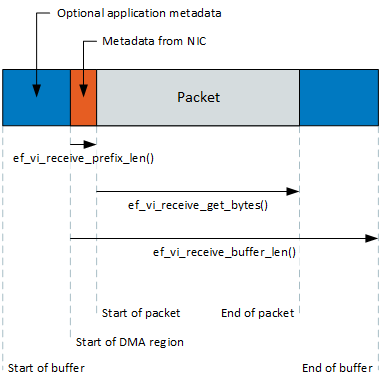
\includegraphics[width=\textwidth,height=\textheight/2,keepaspectratio=true]{packet_buffers_layout_merged.png}
\doxyfigcaption{Layout and functions for RX event merging}
\end{DoxyImage}


If consecutive single-\/buffer packets are received, they can be merged\+:

  
\begin{DoxyImage}
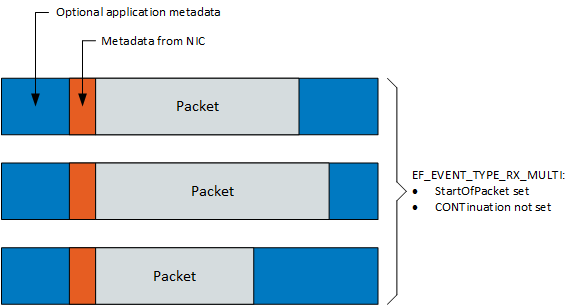
\includegraphics[width=\textwidth,height=\textheight/2,keepaspectratio=true]{packet_buffers_non-jumbo_merged.png}
\doxyfigcaption{RX event merging for non-\/jumbo packets}
\end{DoxyImage}


For a two-\/buffer jumbo packet, the events have different flags, and so cannot be merged\+:

  
\begin{DoxyImage}
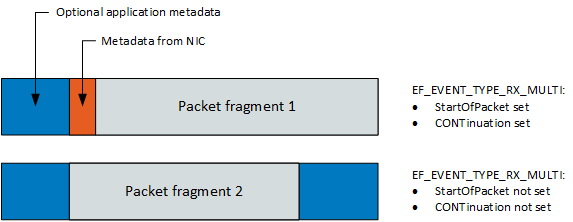
\includegraphics[width=\textwidth,height=\textheight/2,keepaspectratio=true]{packet_buffers_jumbo-2_merged.png}
\doxyfigcaption{RX event merging for a 2-\/buffer jumbo packet}
\end{DoxyImage}


For a larger {\itshape N}-\/buffer jumbo packet, the events for the middle buffers have the same flags, and so can be merged\+:

  
\begin{DoxyImage}
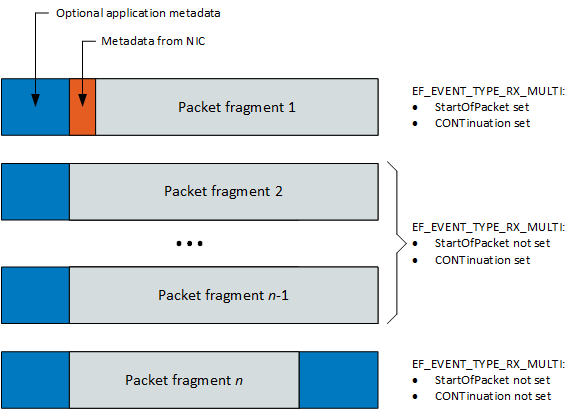
\includegraphics[width=\textwidth,height=\textheight/2,keepaspectratio=true]{packet_buffers_jumbo-n_merged.png}
\doxyfigcaption{Event merging for an \+\_\+\+N\+\_\+-\/buffer jumbo packet}
\end{DoxyImage}


So for jumbo packets, the following multiple events are typically raised\+:


\begin{DoxyEnumerate}
\item An event with {\ttfamily EF\+\_\+\+EVENT\+\_\+\+RX\+\_\+\+MULTI\+\_\+\+SOP} and {\ttfamily EF\+\_\+\+EVENT\+\_\+\+RX\+\_\+\+MULTI\+\_\+\+CONT} containing the first buffer. \mbox{\hyperlink{ef__vi_8h_a7acdfde8e503ed210170ba45874068f3}{ef\+\_\+vi\+\_\+receive\+\_\+get\+\_\+bytes()}} gives the length of the whole jumbo packet.
\item If there are more than two buffers, event(s) with {\ttfamily EF\+\_\+\+EVENT\+\_\+\+RX\+\_\+\+MULTI\+\_\+\+CONT} containing the middle buffers.
\item An event with {\ttfamily ! EF\+\_\+\+EVENT\+\_\+\+RX\+\_\+\+MULTI\+\_\+\+SOP} and {\ttfamily ! EF\+\_\+\+EVENT\+\_\+\+RX\+\_\+\+MULTI\+\_\+\+CONT} containing the final buffer. The length of the payload can be inferred based on the total length of the Jumbo packet minus the lengths of previous payloads.
\end{DoxyEnumerate}

There is example code in the following locations\+:


\begin{DoxyItemize}
\item the \mbox{\hyperlink{applications_efsink}{efsink}} example application
\item the handle\+\_\+rx\+\_\+scatter\+\_\+merge() function within {\ttfamily openonload/src/lib/transport/ip/netif\+\_\+event.\+c}.
\end{DoxyItemize}\hypertarget{using_using_filters}{}\doxysection{Adding Filters}\label{using_using_filters}
Filters are the means by which the adapter decides where to deliver packets it receives from the network. By default all packets are delivered to the kernel network stack. Filters are added by an ef\+\_\+vi application to direct received packets to a given virtual interface.


\begin{DoxyItemize}
\item If a filter cannot be added, for example because an incompatible filter already exists, an error is returned.
\item By default the \textquotesingle{}all\textquotesingle{} filters are sending everything to the kernel. They are equivalent to setting promiscuous mode on the NIC.
\item On SFN5000 and SFN6000 series NICs each filter can only exist for one virtual interface, and so each packet which arrives can be forwarded only to a single application (unless two applications share a stack). Only the first application to insert a specific filter will succeed; other applications will then get an error.

Note that this includes filters inserted both by other ef\+\_\+vi applications and by Onload -\/ which typically uses only fully connected and listen filters.
\item The SFN7000 and SFN8000 series NICs are not subject to this restriction. If two applications insert the same multicast filter, a copy of the packets is delivered to each application and applications remain unaware of each other.
\item IP filters do not match IP fragments, which are therefore received by the kernel stack. If this is an issue, layer 2 filters should be installed by the user.
\item There are no ranges, or other local wildcard support. To filter on a range of values, one of the following is required\+:
\begin{DoxyItemize}
\item insert multiple filters, one per value in the range (NICs support upwards of a thousand filters easily)
\item have the interesting traffic sent to a specific MAC address, and use a MAC address filter
\item have the interesting traffic sent to a specific VLAN, and use a VLAN filter.
\end{DoxyItemize}
\item Cookies are used to remove filters.
\item De-\/allocating a virtual interface removes any filters set for the virtual interface.
\end{DoxyItemize}

Filters are checked in the following order, which is roughly most-\/specific first\+:
\begin{DoxyEnumerate}
\item Fully connected TCP/\+UDP. (Specifies local and remote port and IP)
\item Listen socket. (Specifies local port and IP, but allows any remote IP/port)
\item Destination MAC address, and optionally VLAN. (Useful for multicast reception, though IP can be used instead if preferred. Also useful for custom protocols.)
\item Everything else. (All unicast, all multicast.)
\end{DoxyEnumerate}


\begin{DoxyCode}{0}
\DoxyCodeLine{\textcolor{keywordtype}{void} \mbox{\hyperlink{vi_8h_a2195efb4c62ebcf9c98c04bcbc842979}{ef\_filter\_spec\_init}}(\mbox{\hyperlink{structef__filter__spec}{ef\_filter\_spec}}* fs,}
\DoxyCodeLine{                         \textcolor{keyword}{enum} \mbox{\hyperlink{vi_8h_ae25195780aad9dcfb218728db965a8b6}{ef\_filter\_flags}} flags);}
\DoxyCodeLine{}
\DoxyCodeLine{\textcolor{keywordtype}{int} \mbox{\hyperlink{vi_8h_a1d04a4feb412f3584ffb8eeb36207912}{ef\_filter\_spec\_set\_ip4\_local}}(\mbox{\hyperlink{structef__filter__spec}{ef\_filter\_spec}}* fs,}
\DoxyCodeLine{                                 \textcolor{keywordtype}{int} protocol,}
\DoxyCodeLine{                                 \textcolor{keywordtype}{unsigned} host\_be32, \textcolor{keywordtype}{int} port\_be16);}
\DoxyCodeLine{}
\DoxyCodeLine{\textcolor{keywordtype}{int} \mbox{\hyperlink{vi_8h_ae91372fd3996c517136a236ef0669db5}{ef\_filter\_spec\_set\_ip4\_full}}(\mbox{\hyperlink{structef__filter__spec}{ef\_filter\_spec}}* fs,}
\DoxyCodeLine{                                \textcolor{keywordtype}{int} protocol,}
\DoxyCodeLine{                                \textcolor{keywordtype}{unsigned} host\_be32, \textcolor{keywordtype}{int} port\_be16,}
\DoxyCodeLine{                                \textcolor{keywordtype}{unsigned} rhost\_be32, \textcolor{keywordtype}{int} rport\_be16);}
\DoxyCodeLine{}
\DoxyCodeLine{\textcolor{keywordtype}{int} \mbox{\hyperlink{vi_8h_a5f8e4fb095dc588c49cfcbc064ef7810}{ef\_filter\_spec\_set\_vlan}}(\mbox{\hyperlink{structef__filter__spec}{ef\_filter\_spec}}* fs,}
\DoxyCodeLine{                            \textcolor{keywordtype}{int} vlan\_id);}
\DoxyCodeLine{}
\DoxyCodeLine{\textcolor{keywordtype}{int} \mbox{\hyperlink{vi_8h_af528ebfe9024176f75d55a7733552435}{ef\_filter\_spec\_set\_eth\_local}}(\mbox{\hyperlink{structef__filter__spec}{ef\_filter\_spec}}* fs,}
\DoxyCodeLine{                                 \textcolor{keywordtype}{int} vlan\_id,}
\DoxyCodeLine{                                 \textcolor{keyword}{const} \textcolor{keywordtype}{void} *mac);}
\DoxyCodeLine{}
\DoxyCodeLine{\textcolor{keywordtype}{int} \mbox{\hyperlink{vi_8h_a7ebf6ecc2966a4b88367cc274a717417}{ef\_filter\_spec\_set\_unicast\_all}}(\mbox{\hyperlink{structef__filter__spec}{ef\_filter\_spec}}* fs);}
\DoxyCodeLine{}
\DoxyCodeLine{\textcolor{keywordtype}{int} \mbox{\hyperlink{vi_8h_a0c7d3ebf1cc5c5f318ac18ff0c1ff914}{ef\_filter\_spec\_set\_multicast\_all}}(\mbox{\hyperlink{structef__filter__spec}{ef\_filter\_spec}}* fs);}
\DoxyCodeLine{}
\DoxyCodeLine{\textcolor{keywordtype}{int} \mbox{\hyperlink{vi_8h_a6a8a8227b658a5d93548818a45445815}{ef\_filter\_spec\_set\_unicast\_mismatch}}(\mbox{\hyperlink{structef__filter__spec}{ef\_filter\_spec}}* fs);}
\DoxyCodeLine{}
\DoxyCodeLine{\textcolor{keywordtype}{int} \mbox{\hyperlink{vi_8h_af58cc298c09a1337a0118f39f27b9845}{ef\_filter\_spec\_set\_multicast\_mismatch}}(\mbox{\hyperlink{structef__filter__spec}{ef\_filter\_spec}}* fs);}
\DoxyCodeLine{}
\DoxyCodeLine{\textcolor{keywordtype}{int} \mbox{\hyperlink{vi_8h_a377a64780b4b9e9fd01fd7c79dd36edb}{ef\_filter\_spec\_set\_port\_sniff}}(\mbox{\hyperlink{structef__filter__spec}{ef\_filter\_spec}}* fs,}
\DoxyCodeLine{                                  \textcolor{keywordtype}{int} promiscuous);}
\DoxyCodeLine{}
\DoxyCodeLine{\textcolor{keywordtype}{int} \mbox{\hyperlink{vi_8h_a85d2fd83f222962b65890b29193b1618}{ef\_filter\_spec\_set\_tx\_port\_sniff}}(\mbox{\hyperlink{structef__filter__spec}{ef\_filter\_spec}}* fs);}
\DoxyCodeLine{}
\DoxyCodeLine{\textcolor{keywordtype}{int} \mbox{\hyperlink{vi_8h_ab2eff00234093a967c29f57a727af98a}{ef\_filter\_spec\_set\_block\_kernel}}(\mbox{\hyperlink{structef__filter__spec}{ef\_filter\_spec}}* fs);}
\DoxyCodeLine{}
\DoxyCodeLine{\textcolor{keywordtype}{int} \mbox{\hyperlink{vi_8h_ab0f191fe076d51ef701e4d1b2709e4b1}{ef\_filter\_spec\_set\_block\_kernel\_multicast}}(\mbox{\hyperlink{structef__filter__spec}{ef\_filter\_spec}}* fs);}
\DoxyCodeLine{}
\DoxyCodeLine{\textcolor{keywordtype}{int} \mbox{\hyperlink{vi_8h_ae8128e39ce98e1f64a54cba31bae14d0}{ef\_filter\_spec\_set\_block\_kernel\_unicast}}(\mbox{\hyperlink{structef__filter__spec}{ef\_filter\_spec}}* fs);}
\DoxyCodeLine{}
\DoxyCodeLine{\textcolor{keywordtype}{int} \mbox{\hyperlink{vi_8h_a71909d1557f3064579781604fc117e4e}{ef\_vi\_filter\_add}}(\mbox{\hyperlink{structef__vi}{ef\_vi}}* vi,\mbox{\hyperlink{base_8h_afcca014c719554b834e89f0c30e87561}{ef\_driver\_handle}} dh,}
\DoxyCodeLine{                     \textcolor{keyword}{const} \mbox{\hyperlink{structef__filter__spec}{ef\_filter\_spec}}* fs,}
\DoxyCodeLine{                     \mbox{\hyperlink{structef__filter__cookie}{ef\_filter\_cookie}}* filter\_cookie\_out);}
\DoxyCodeLine{}
\DoxyCodeLine{\textcolor{keywordtype}{int} \mbox{\hyperlink{vi_8h_a42f633c2483fb182434c8f7f3ea732fd}{ef\_vi\_filter\_del}}(\mbox{\hyperlink{structef__vi}{ef\_vi}}* vi, \mbox{\hyperlink{base_8h_afcca014c719554b834e89f0c30e87561}{ef\_driver\_handle}} dh,}
\DoxyCodeLine{                     \mbox{\hyperlink{structef__filter__cookie}{ef\_filter\_cookie}}* filter\_cookie);}
\DoxyCodeLine{}
\DoxyCodeLine{\textcolor{keywordtype}{int} \mbox{\hyperlink{vi_8h_a89aa0805536fccbaf79c2120c316ff65}{ef\_vi\_set\_filter\_add}}(\mbox{\hyperlink{structef__vi__set}{ef\_vi\_set}}*,}
\DoxyCodeLine{                        \mbox{\hyperlink{base_8h_afcca014c719554b834e89f0c30e87561}{ef\_driver\_handle}} dh,}
\DoxyCodeLine{                        \textcolor{keyword}{const} \mbox{\hyperlink{structef__filter__spec}{ef\_filter\_spec}}* fs,}
\DoxyCodeLine{                        \mbox{\hyperlink{structef__filter__cookie}{ef\_filter\_cookie}}* filter\_cookie\_out);}
\DoxyCodeLine{}
\DoxyCodeLine{\textcolor{keywordtype}{int} \mbox{\hyperlink{vi_8h_ad2bce41b1eccaa8c393c9abacab9905c}{ef\_vi\_set\_filter\_del}}(\mbox{\hyperlink{structef__vi__set}{ef\_vi\_set}}*, \mbox{\hyperlink{base_8h_afcca014c719554b834e89f0c30e87561}{ef\_driver\_handle}} dh,}
\DoxyCodeLine{                         \mbox{\hyperlink{structef__filter__cookie}{ef\_filter\_cookie}}* filter\_cookie);}

\end{DoxyCode}
 {\bfseries{Figure\+: Creating Filters}}\hypertarget{using_filters_permission}{}\doxysubsection{Filter permission requirements}\label{using_filters_permission}
Super-\/user rights (specifically {\ttfamily CAP\+\_\+\+NET\+\_\+\+ADMIN}) are needed to use the following filters\+:


\begin{DoxyItemize}
\item IP proto (and the VLAN variant)
\item Ethertype (and the VLAN variant)
\item Unicast-\/mismatch (and the VLAN variant)
\item Multicast-\/mismatch (and the VLAN variant)
\item Unicast-\/all
\item Multicast-\/all
\item Kernel block
\item Sniff.
\end{DoxyItemize}\hypertarget{using_filters_variant}{}\doxysubsection{Filters available per Firmware Variant}\label{using_filters_variant}
The kernel will install a destination MAC address filter for each Solarflare interface. The kernel will install a broadcast MAC address filter for each Solarflare interface.

A broadcast MAC address is treated like any other MAC address. Multiple applications can insert the same filter and all will receive a copy of the received traffic.

As a rule, more-\/specific filters will capture traffic over less-\/specific filters.

When the Solarflare adapter is configured to use the full\+\_\+featured firmware variant, the following combinations of ef\+\_\+filter\+\_\+spec\+\_\+set\+\_\+$\ast$() calls are supported, and are applied in this order\+:


\begin{DoxyItemize}
\item \mbox{\hyperlink{vi_8h_ae91372fd3996c517136a236ef0669db5}{ef\+\_\+filter\+\_\+spec\+\_\+set\+\_\+ip4\+\_\+full()}} or \mbox{\hyperlink{vi_8h_a90dde88cfc07177f35be74c77cfb9e40}{ef\+\_\+filter\+\_\+spec\+\_\+set\+\_\+ip6\+\_\+full()}}
\item \mbox{\hyperlink{vi_8h_a9f8fcdc598fa4971ea44ca765de4d51c}{ef\+\_\+filter\+\_\+spec\+\_\+set\+\_\+eth\+\_\+type()}}
\item \mbox{\hyperlink{vi_8h_af528ebfe9024176f75d55a7733552435}{ef\+\_\+filter\+\_\+spec\+\_\+set\+\_\+eth\+\_\+local()}}
\item optionally, \mbox{\hyperlink{vi_8h_a5f8e4fb095dc588c49cfcbc064ef7810}{ef\+\_\+filter\+\_\+spec\+\_\+set\+\_\+vlan()}} ~\newline
~\newline

\item \mbox{\hyperlink{vi_8h_a1d04a4feb412f3584ffb8eeb36207912}{ef\+\_\+filter\+\_\+spec\+\_\+set\+\_\+ip4\+\_\+local()}} or \mbox{\hyperlink{vi_8h_a33228093a9326e0606581ce03260dc76}{ef\+\_\+filter\+\_\+spec\+\_\+set\+\_\+ip6\+\_\+local()}}
\item \mbox{\hyperlink{vi_8h_a9f8fcdc598fa4971ea44ca765de4d51c}{ef\+\_\+filter\+\_\+spec\+\_\+set\+\_\+eth\+\_\+type()}}
\item \mbox{\hyperlink{vi_8h_af528ebfe9024176f75d55a7733552435}{ef\+\_\+filter\+\_\+spec\+\_\+set\+\_\+eth\+\_\+local()}}
\item optionally, \mbox{\hyperlink{vi_8h_a5f8e4fb095dc588c49cfcbc064ef7810}{ef\+\_\+filter\+\_\+spec\+\_\+set\+\_\+vlan()}} ~\newline
~\newline

\item \mbox{\hyperlink{vi_8h_af528ebfe9024176f75d55a7733552435}{ef\+\_\+filter\+\_\+spec\+\_\+set\+\_\+eth\+\_\+local()}}
\item optionally, \mbox{\hyperlink{vi_8h_a5f8e4fb095dc588c49cfcbc064ef7810}{ef\+\_\+filter\+\_\+spec\+\_\+set\+\_\+vlan()}} ~\newline
~\newline

\item \mbox{\hyperlink{vi_8h_a6a8a8227b658a5d93548818a45445815}{ef\+\_\+filter\+\_\+spec\+\_\+set\+\_\+unicast\+\_\+mismatch()}}
\item optionally, \mbox{\hyperlink{vi_8h_a5f8e4fb095dc588c49cfcbc064ef7810}{ef\+\_\+filter\+\_\+spec\+\_\+set\+\_\+vlan()}} ~\newline
~\newline

\item \mbox{\hyperlink{vi_8h_af58cc298c09a1337a0118f39f27b9845}{ef\+\_\+filter\+\_\+spec\+\_\+set\+\_\+multicast\+\_\+mismatch()}}
\item optionally, \mbox{\hyperlink{vi_8h_a5f8e4fb095dc588c49cfcbc064ef7810}{ef\+\_\+filter\+\_\+spec\+\_\+set\+\_\+vlan()}}
\end{DoxyItemize}

When the Solarflare adapter is configured to use the low\+\_\+latency firmware variant, the following combinations of ef\+\_\+filter\+\_\+spec\+\_\+set\+\_\+$\ast$() calls are supported, and are applied in this order\+:


\begin{DoxyItemize}
\item \mbox{\hyperlink{vi_8h_ae91372fd3996c517136a236ef0669db5}{ef\+\_\+filter\+\_\+spec\+\_\+set\+\_\+ip4\+\_\+full()}} or \mbox{\hyperlink{vi_8h_a90dde88cfc07177f35be74c77cfb9e40}{ef\+\_\+filter\+\_\+spec\+\_\+set\+\_\+ip6\+\_\+full()}}
\item \mbox{\hyperlink{vi_8h_a9f8fcdc598fa4971ea44ca765de4d51c}{ef\+\_\+filter\+\_\+spec\+\_\+set\+\_\+eth\+\_\+type()}} ~\newline
~\newline

\item \mbox{\hyperlink{vi_8h_a1d04a4feb412f3584ffb8eeb36207912}{ef\+\_\+filter\+\_\+spec\+\_\+set\+\_\+ip4\+\_\+local()}} or \mbox{\hyperlink{vi_8h_a33228093a9326e0606581ce03260dc76}{ef\+\_\+filter\+\_\+spec\+\_\+set\+\_\+ip6\+\_\+local()}}
\item \mbox{\hyperlink{vi_8h_a9f8fcdc598fa4971ea44ca765de4d51c}{ef\+\_\+filter\+\_\+spec\+\_\+set\+\_\+eth\+\_\+type()}} ~\newline
~\newline

\item \mbox{\hyperlink{vi_8h_af528ebfe9024176f75d55a7733552435}{ef\+\_\+filter\+\_\+spec\+\_\+set\+\_\+eth\+\_\+local()}}
\item optionally, \mbox{\hyperlink{vi_8h_a5f8e4fb095dc588c49cfcbc064ef7810}{ef\+\_\+filter\+\_\+spec\+\_\+set\+\_\+vlan()}} ~\newline
~\newline

\item \mbox{\hyperlink{vi_8h_a6a8a8227b658a5d93548818a45445815}{ef\+\_\+filter\+\_\+spec\+\_\+set\+\_\+unicast\+\_\+mismatch()}} ~\newline
~\newline

\item \mbox{\hyperlink{vi_8h_af58cc298c09a1337a0118f39f27b9845}{ef\+\_\+filter\+\_\+spec\+\_\+set\+\_\+multicast\+\_\+mismatch()}}
\end{DoxyItemize}

When the Solarflare adapter is configured to use the packed\+\_\+stream firmware variant, the following combinations of ef\+\_\+filter\+\_\+spec\+\_\+set\+\_\+$\ast$() calls are supported, and are applied in this order\+:


\begin{DoxyItemize}
\item \mbox{\hyperlink{vi_8h_a1d04a4feb412f3584ffb8eeb36207912}{ef\+\_\+filter\+\_\+spec\+\_\+set\+\_\+ip4\+\_\+local()}} or \mbox{\hyperlink{vi_8h_a33228093a9326e0606581ce03260dc76}{ef\+\_\+filter\+\_\+spec\+\_\+set\+\_\+ip6\+\_\+local()}}
\item \mbox{\hyperlink{vi_8h_a9f8fcdc598fa4971ea44ca765de4d51c}{ef\+\_\+filter\+\_\+spec\+\_\+set\+\_\+eth\+\_\+type()}} ~\newline
~\newline

\item \mbox{\hyperlink{vi_8h_af528ebfe9024176f75d55a7733552435}{ef\+\_\+filter\+\_\+spec\+\_\+set\+\_\+eth\+\_\+local()}} ~\newline
~\newline

\item \mbox{\hyperlink{vi_8h_a6a8a8227b658a5d93548818a45445815}{ef\+\_\+filter\+\_\+spec\+\_\+set\+\_\+unicast\+\_\+mismatch()}}
\item optionally, \mbox{\hyperlink{vi_8h_a5f8e4fb095dc588c49cfcbc064ef7810}{ef\+\_\+filter\+\_\+spec\+\_\+set\+\_\+vlan()}} ~\newline
~\newline

\item \mbox{\hyperlink{vi_8h_af58cc298c09a1337a0118f39f27b9845}{ef\+\_\+filter\+\_\+spec\+\_\+set\+\_\+multicast\+\_\+mismatch()}}
\item optionally, \mbox{\hyperlink{vi_8h_a5f8e4fb095dc588c49cfcbc064ef7810}{ef\+\_\+filter\+\_\+spec\+\_\+set\+\_\+vlan()}}
\end{DoxyItemize}\hypertarget{using_using_igmp}{}\doxysection{IGMP subscriptions}\label{using_using_igmp}
In theory it is possible to generate IGMP join/leave messages and send them via ef\+\_\+vi. For reliable operation this would mean re-\/implementing the whole IGMP protocol. As the IGMP messages are not especially latency sensitive, this would be a lot of work for minimal benefit.

A common solution when using ef\+\_\+vi to receive multicast is to also create a standard UDP socket and use IP\+\_\+\+ADD\+\_\+\+MEMBERSHIP/\+IP\+\_\+\+DROP\+\_\+\+MEMBERSHIP to control the multicast groups for the interface. The kernel stack will then generate and respond to the IGMP messages as normal. This UDP socket should not be accelerated using Onload, which can be achieved by using onload\+\_\+socket\+\_\+nonaccel() to create this socket.

\begin{DoxyNote}{Note}
The onload\+\_\+socket\+\_\+nonaccel() function is a part of the Onload Extensions API, and is documented in the {\itshape Onload User Guide}.
\end{DoxyNote}
If the ef\+\_\+vi application installs filters for individual UDP ports then everything will work fine. Once the VI has a UDP filter installed for the multicast traffic, this filter will match the received traffic in preference to the MAC multicast address filter installed by the kernel stack. Consequently, the UDP socket won\textquotesingle{}t see the actual traffic, but the VI will. The IGMP messages will not match the ef\+\_\+vi filter, and so IGMP will still be handled by the kernel stack. If the traffic rate is high, then it is best to install the filter on the VI before joining the group, and to close the UDP socket before removing the filter or closing the VI. This prevents the UDP socket receiving lots of unwanted traffic.

If the ef\+\_\+vi application installs the \char`\"{}multicast-\/all\char`\"{} filter for the VI, then this will normally consume all multicast traffic on the interface. This would potentially include IGMP messages, which could cause the subscriptions to fail. In this case, an extra filter entry can be added to redirect all incoming IGMP packets to the kernel stack, so that they can still be processed by the kernel\+:


\begin{DoxyCode}{0}
\DoxyCodeLine{ethtool -\/U <interface> flow-\/type ip4 l4proto 2 vlan 0 m 0xf000 action 0}

\end{DoxyCode}
\hypertarget{using_using_freeing}{}\doxysection{Freeing Resources}\label{using_using_freeing}
Users of ef\+\_\+vi must do the following to free resources\+:
\begin{DoxyEnumerate}
\item Release and free memory regions by calling \mbox{\hyperlink{memreg_8h_a50faeb36b707ebf538b789d9f311642f}{ef\+\_\+memreg\+\_\+free()}}.
\item Release and free a virtual interface by calling \mbox{\hyperlink{vi_8h_ac9c8bc0bab4933eb9a3448a025209f3f}{ef\+\_\+vi\+\_\+free()}}.
\item Release and free a protection domain by calling \mbox{\hyperlink{pd_8h_a74417cfe9364bda64435834a8086b91f}{ef\+\_\+pd\+\_\+free()}}.
\item Close a driver handle by calling \mbox{\hyperlink{base_8h_ac7afa09b92436d8007255c3a8723c759}{ef\+\_\+driver\+\_\+close()}}.
\end{DoxyEnumerate}


\begin{DoxyCode}{0}
\DoxyCodeLine{\textcolor{comment}{/* Release and free a memory region */}}
\DoxyCodeLine{\textcolor{keywordtype}{int} \mbox{\hyperlink{memreg_8h_a50faeb36b707ebf538b789d9f311642f}{ef\_memreg\_free}}(\mbox{\hyperlink{structef__memreg}{ef\_memreg}}* mr,}
\DoxyCodeLine{                   \mbox{\hyperlink{base_8h_afcca014c719554b834e89f0c30e87561}{ef\_driver\_handle}} mr\_dh);}

\end{DoxyCode}
 {\bfseries{Figure\+: Release and Free a Memory Region}}


\begin{DoxyCode}{0}
\DoxyCodeLine{\textcolor{comment}{/* Release and free a virtual interface */}}
\DoxyCodeLine{\textcolor{keywordtype}{int} \mbox{\hyperlink{vi_8h_ac9c8bc0bab4933eb9a3448a025209f3f}{ef\_vi\_free}}(\mbox{\hyperlink{structef__vi}{ef\_vi}}* vi,}
\DoxyCodeLine{               \mbox{\hyperlink{base_8h_afcca014c719554b834e89f0c30e87561}{ef\_driver\_handle}} vi\_dh);}

\end{DoxyCode}
 {\bfseries{Figure\+: Release and Free a Virtual Interface}}


\begin{DoxyCode}{0}
\DoxyCodeLine{\textcolor{comment}{/* Release and free a protection domain */}}
\DoxyCodeLine{\textcolor{keywordtype}{int} \mbox{\hyperlink{pd_8h_a74417cfe9364bda64435834a8086b91f}{ef\_pd\_free}}(\mbox{\hyperlink{structef__pd}{ef\_pd}} *pd,}
\DoxyCodeLine{               \mbox{\hyperlink{base_8h_afcca014c719554b834e89f0c30e87561}{ef\_driver\_handle}} pd\_dh);}

\end{DoxyCode}
 {\bfseries{Figure\+: Release and Free a Protection Domain}}\hypertarget{using_design}{}\doxysection{Design Considerations}\label{using_design}
This section outlines some considerations that are required when designing an ef\+\_\+vi application.\hypertarget{using_interrupts}{}\doxysubsection{Interrupts}\label{using_interrupts}
Interrupts are not enabled by ef\+\_\+vi by default.

Interrupts are enabled only if \mbox{\hyperlink{base_8h_a282e0ba3717d2e509cd4ebc984f62461}{ef\+\_\+eventq\+\_\+wait()}} is called. If there are no events immediately ready, then this function will enable an interrupt, and sleep until that interrupt fires. Interrupts are then disabled again.\hypertarget{using_thread_safety}{}\doxysubsection{Thread Safety}\label{using_thread_safety}
There is no thread-\/safety on ef\+\_\+vi functions. This is for speed. If thread-\/safety is required, it must be provided by the ef\+\_\+vi application.

The usual use-\/case is to have multiple virtual interface structures for independent operation. There is then no need to lock.\hypertarget{using_pb_addressing}{}\doxysubsection{Packet Buffer Addressing}\label{using_pb_addressing}
Different configuration modes are available for addressing packet buffers.


\begin{DoxyItemize}
\item {\itshape Network Adapter Buffer Table Mode} uses a block of memory on the adapter to store a translation table mapping between buffer IDs and physical addresses\+:
\begin{DoxyItemize}
\item When using a SFN5000 or SFN6000 series adapter there are 65536 entries in the buffer table. Each entry maps a 4KB page of memory that holds two 2KB packet buffers, and so a maxiumum of 131072 packet buffers are available. The kernel uses some of these, leaving about 120,000 packet buffers available for ef\+\_\+vi.
\item The SFN7000 series adapters have {\itshape Large Buffer Table Support}. Each entry can map a larger region of memory, or a huge page, enabling them to support many more packet buffers without the need to use Scalable Packet Buffer Mode.
\end{DoxyItemize}

This is the default mode.
\item {\itshape Scalable Packet Buffer Mode} allocates packet buffers from the kernel IOMMU. It uses Single Root I/O Virtualization (SR-\/\+IOV) virtual functions (VF) to provide memory protection and translation. This removes the buffer limitation of the buffer table.
\begin{DoxyItemize}
\item SR-\/\+IOV must be enabled
\item the kernel must support an IOMMU.
\end{DoxyItemize}

An ef\+\_\+vi application can enable this mode by setting the environment variable {\ttfamily EF\+\_\+\+VI\+\_\+\+PD\+\_\+\+FLAGS=vf}.
\item {\itshape Physical Addressing Mode} uses actual physical addresses to identify packet buffers. An ef\+\_\+vi application can therefore direct the adapter to access memory that is not in the application address space. For example, this can be used for zero-\/copy from the kernel buffer cache. any piece of memory.

Physical Addressing Mode allows stacks to use large amounts of packet buffer memory, avoiding address translation limitations on some adapters and without the need to configure and use SR-\/\+IOV virtual functions.
\begin{DoxyItemize}
\item No memory protection is provided. Physical addressing mode removes memory protection from the network adapter\textquotesingle{}s access of packet buffers. Unprivileged user-\/level code is provided and directly handles the raw physical memory addresses of packet buffers. User-\/level code provides physical memory addresses directly to the adapter with the ability to read or write arbitrary memory locations.
\item It is important to ensure that packet buffers are page aligned.
\end{DoxyItemize}

An ef\+\_\+vi application can enable this mode by setting the environment variable {\ttfamily EF\+\_\+\+VI\+\_\+\+PD\+\_\+\+FLAGS=phys}.

The sfc\+\_\+char module option must also be enabled in a file in the /etc/modprobe.d directory where N is the integer group ID of the user running the ef\+\_\+vi application. Set to -\/1 means ALL users are permitted access.\+:
\end{DoxyItemize}


\begin{DoxyCode}{0}
\DoxyCodeLine{options sfc\_char phys\_mode\_gid=<N>}

\end{DoxyCode}


For more information about these configuration modes, see the chapter titled {\itshape Packet Buffers} in the {\itshape Onload User Guide} (SF-\/104474-\/\+CD).\hypertarget{using_vm}{}\doxysubsection{Virtual machines}\label{using_vm}
Ef\+\_\+vi can be used in virtual machines provided PCI passthrough is used. With PCI passthrough a slice of the network adapter is mapped directly into the address space of the virtual machine so that device drivers in the VM OS can access the network adapter directly. To isolate VMs from one another and from the hypervisor, I/O addresses are also virtualised. I/O addresses generated by the network adapter are translated to physical memory addresses by the system IOMMU.

When ef\+\_\+vi is used in virtual machines two levels of address translation are performed by default. Firstly a translation from DMA address to I/O address, performed by the adapter to isolate the application from other applications and the kernel. Then a translation from I/O address to physical address by the system IOMMU, isolating the virtual machines. Physical address mode can also be used in virtual machines, in which case the adapter translation is omitted.\hypertarget{using_limitations}{}\doxysection{Known Limitations}\label{using_limitations}
\hypertarget{using_timestamping}{}\doxysubsection{Timestamping}\label{using_timestamping}
When timestamping is enabled, the VI must be polled regularly (even when no packets are available). Timestamps consume four event queue slots per second and failing to poll the VI can result in event queue overflow. When there are no packets to receive, stale timestamps are not returned to the application, but polling ensures that they are cleared from the event queue.\hypertarget{using_fill_level}{}\doxysubsection{Minimum Fill Level}\label{using_fill_level}
You must poll for at least EF\+\_\+\+VI\+\_\+\+EVENT\+\_\+\+POLL\+\_\+\+MIN\+\_\+\+EVS at a time. You will also need to initially fill the RX ring with at least 16 packet buffers to ensure that the card begins acquiring packets. (It\textquotesingle{}s OK to underrun once the application has started; although of course doing so risks drops.)

It\textquotesingle{}s (very slightly) more efficient to refill the ring in batch sizes of 8/16/32 or 64 anyway.\hypertarget{using_using_example}{}\doxysection{Example}\label{using_using_example}
Below is a simple example showing a starting framework for an ef\+\_\+vi application. This is not a complete program. There is no initialization, and much of the other required code is only indicated by comments.


\begin{DoxyCode}{0}
\DoxyCodeLine{\textcolor{keyword}{static} \textcolor{keywordtype}{void} handle\_poll(\mbox{\hyperlink{structef__vi}{ef\_vi}} *vi)}
\DoxyCodeLine{\{}
\DoxyCodeLine{  \mbox{\hyperlink{unionef__event}{ef\_event}} events[POLL\_BATCH\_SIZE];}
\DoxyCodeLine{  \textcolor{keywordtype}{int} n\_ev = \mbox{\hyperlink{ef__vi_8h_ab340116b526f45dd378fe279f0c05a48}{ef\_eventq\_poll}}(\&vi, events, POLL\_BATCH\_SIZE);}
\DoxyCodeLine{  \textcolor{keywordflow}{for}( i = O; i < n\_ev; ++i ) \{}
\DoxyCodeLine{    \textcolor{keywordflow}{switch}( \mbox{\hyperlink{ef__vi_8h_a66c3866ad0c965c4a257a02cbb125388}{EF\_EVENT\_TYPE}}(events[i]) ) \{}
\DoxyCodeLine{    \textcolor{keywordflow}{case} \mbox{\hyperlink{ef__vi_8h_a06fc87d81c62e9abb8790b6e5713c55ba60ca113e8fe79115ba9efe22471a9001}{EF\_EVENT\_TYPE\_RX}}:}
\DoxyCodeLine{      \textcolor{comment}{// Accumulate used buffer}}
\DoxyCodeLine{      \textcolor{keywordflow}{break};}
\DoxyCodeLine{    \textcolor{keywordflow}{case} \mbox{\hyperlink{ef__vi_8h_a06fc87d81c62e9abb8790b6e5713c55ba48528de8329421a4ac7785774bb4c894}{EF\_EVENT\_TYPE\_TX}}:}
\DoxyCodeLine{      \textcolor{comment}{/* Each EF\_EVENT\_TYPE\_TX can signal multiple completed sends */}}
\DoxyCodeLine{      \textcolor{keywordtype}{int} num\_completed = \mbox{\hyperlink{ef__vi_8h_a03c43da4cdac5419b1d859b20854ec37}{ef\_vi\_transmit\_unbundle}}(vi, events[i], \&dma\_id);}
\DoxyCodeLine{      \textcolor{keywordflow}{break};}
\DoxyCodeLine{    \textcolor{keywordflow}{case} \mbox{\hyperlink{ef__vi_8h_a06fc87d81c62e9abb8790b6e5713c55ba117a208b3f2e58062cc505b88f984057}{EF\_EVENT\_TYPE\_RX\_DISCARD}}:}
\DoxyCodeLine{    \textcolor{keywordflow}{case} \mbox{\hyperlink{ef__vi_8h_a06fc87d81c62e9abb8790b6e5713c55ba8f7d923defae51d9d8c226b51c51d56d}{EF\_EVENT\_TYPE\_RX\_NO\_DESC\_TRUNC}}:}
\DoxyCodeLine{      \textcolor{comment}{/* Discard events also use up buffers */}}
\DoxyCodeLine{      \textcolor{comment}{// Accumulate buffer in user space}}
\DoxyCodeLine{      \textcolor{keywordflow}{break};}
\DoxyCodeLine{    \textcolor{keywordflow}{default}:}
\DoxyCodeLine{      \textcolor{comment}{/* Other error types */}}
\DoxyCodeLine{    \}}
\DoxyCodeLine{  \}}
\DoxyCodeLine{\}}
\DoxyCodeLine{}
\DoxyCodeLine{\textcolor{keyword}{static} \textcolor{keywordtype}{void} refill\_rx\_ring(\mbox{\hyperlink{structef__vi}{ef\_vi}} *vi)}
\DoxyCodeLine{\{}
\DoxyCodeLine{  \textcolor{keywordflow}{if}( \mbox{\hyperlink{ef__vi_8h_a4ce37375952e8174b39ec2025955122f}{ef\_vi\_receive\_space}}(\&vi) < REFILL\_BATCH\_SIZE )}
\DoxyCodeLine{    \textcolor{keywordflow}{return};}
\DoxyCodeLine{  \textcolor{keywordtype}{int} refill\_count = REFILL\_BATCH\_SIZE;}
\DoxyCodeLine{  \textcolor{comment}{/* Falling too low? */}}
\DoxyCodeLine{  \textcolor{keywordflow}{if}( \mbox{\hyperlink{ef__vi_8h_a4ce37375952e8174b39ec2025955122f}{ef\_vi\_receive\_space}}(\&vi) > \mbox{\hyperlink{ef__vi_8h_aa1d1b37d9e0352d4f2eacbbbe535f59e}{ef\_vi\_receive\_capacity}}(\&vi) / 2 )}
\DoxyCodeLine{    refill\_count = \mbox{\hyperlink{ef__vi_8h_a4ce37375952e8174b39ec2025955122f}{ef\_vi\_receive\_space}}(\&vi);}
\DoxyCodeLine{  \textcolor{comment}{/* Enough free buffers? */}}
\DoxyCodeLine{  \textcolor{keywordflow}{if}( refill\_count > free\_bufs\_in\_sw )}
\DoxyCodeLine{    refill\_count = free\_bufs\_in\_sw;}
\DoxyCodeLine{  \textcolor{comment}{/* Round down to batch size */}}
\DoxyCodeLine{  refill\_count \&= \string~(REFILL\_BATCH\_SIZE -\/ 1);}
\DoxyCodeLine{  \textcolor{keywordflow}{if}( refill\_count ) \{}
\DoxyCodeLine{    \textcolor{keywordflow}{while}( refill\_count ) \{}
\DoxyCodeLine{      \mbox{\hyperlink{ef__vi_8h_a9e1fbd2c66475fde3aa1b7df19841ef9}{ef\_vi\_receive\_init}}(...);}
\DoxyCodeLine{      -\/-\/refill\_count;}
\DoxyCodeLine{    \}}
\DoxyCodeLine{    \mbox{\hyperlink{ef__vi_8h_abcd5dc1be7ff1e9f9a4a84df86305099}{ef\_vi\_receive\_push}}(\&vi);}
\DoxyCodeLine{  \}}
\DoxyCodeLine{\}}
\DoxyCodeLine{}
\DoxyCodeLine{\textcolor{keywordtype}{int} main(\textcolor{keywordtype}{int} argc, \textcolor{keywordtype}{char} argv[]) (}
\DoxyCodeLine{  \textcolor{keywordflow}{while}( 1 ) \{}
\DoxyCodeLine{    poll\_events(\&vi);}
\DoxyCodeLine{    refill\_rx\_ring(\&vi);}
\DoxyCodeLine{  \}}
\DoxyCodeLine{\}}

\end{DoxyCode}
 
\chapter{Worked Example}
\label{example}
\Hypertarget{example}
This part of the documentation examines a simplified version of \mbox{\hyperlink{applications_eflatency}{eflatency}}. This is a small application which listens for packets and replies, with as low latency as possible.

This documentation discusses the tradeoffs that have been chosen, some performance issues to avoid, and some possible additions that have been omitted for clarity.

See also the supplied code for \mbox{\hyperlink{applications_eflatency}{eflatency}} , which includes many of these improvements.\hypertarget{example_example_setup}{}\doxysection{Setup}\label{example_example_setup}
The first step is to set up ef\+\_\+vi\+:
\begin{DoxyItemize}
\item \#include the various headers we need (\mbox{\hyperlink{pd_8h}{etherfabric/pd.\+h}}, \mbox{\hyperlink{vi_8h}{vi.\+h}}, \mbox{\hyperlink{memreg_8h}{memreg.\+h}})
\item open the driver
\item allocate a protection domain
\item allocate a virtual interface from the protection domain.
\end{DoxyItemize}


\begin{DoxyCode}{0}
\DoxyCodeLine{\mbox{\hyperlink{base_8h_afcca014c719554b834e89f0c30e87561}{ef\_driver\_handle}}  driver\_handle;}
\DoxyCodeLine{\mbox{\hyperlink{structef__vi}{ef\_vi}}             vi;}
\DoxyCodeLine{\mbox{\hyperlink{structef__pd}{ef\_pd}}             pd;}
\DoxyCodeLine{\textcolor{keyword}{static} \textcolor{keywordtype}{void} do\_init(\textcolor{keywordtype}{int} ifindex)\{}
\DoxyCodeLine{  \mbox{\hyperlink{base_8h_acb2b46854a36c5eb295878d306a274d2}{ef\_driver\_open}}(\&driver\_handle);}
\DoxyCodeLine{  \mbox{\hyperlink{pd_8h_a65e7675bc0fb9da9551c83ada8b4b995}{ef\_pd\_alloc}}(\&pd, driver\_handle, ifindex, \mbox{\hyperlink{pd_8h_a09263cdade29abed15a6775debbf27d9aee8bd6800bf8bd7b9af02e9b19663ea9}{EF\_PD\_DEFAULT}} );}
\DoxyCodeLine{  \mbox{\hyperlink{vi_8h_a66124c16b919445b44e2bcba50dbc344}{ef\_vi\_alloc\_from\_pd}}(\&vi, driver\_handle, \&pd, driver\_handle,}
\DoxyCodeLine{                      -\/1, -\/1, -\/1, NULL, -\/1, 0);}

\end{DoxyCode}


The following improvements could be made\+:
\begin{DoxyItemize}
\item check the return values from these functions, in case the card has run out of resources and is unable to allocate more virtual interfaces
\item offer physical buffer mode here.
\end{DoxyItemize}\hypertarget{example_example_buffers}{}\doxysection{Creating Packet buffers}\label{example_example_buffers}
The next step is to allocate a memory region and register it for packet buffers.


\begin{DoxyCode}{0}
\DoxyCodeLine{\textcolor{keyword}{const} \textcolor{keywordtype}{int} BUF\_SIZE = 2048;  \textcolor{comment}{/* Hardware always wants 2k buffers */}}
\DoxyCodeLine{\textcolor{keywordtype}{int} bytes = N\_BUFS * BUF\_SIZE;}
\DoxyCodeLine{\textcolor{keywordtype}{void}* p;}
\DoxyCodeLine{posix\_memalign(\&p, 4096, bytes)  \textcolor{comment}{/* allocate aligned memory */}}
\DoxyCodeLine{\mbox{\hyperlink{memreg_8h_ad802d1d7c6487fbeeff8ed682caf71c8}{ef\_memreg\_alloc}}(\&memreg, driver\_handle, \&pd, driver\_handle,}
\DoxyCodeLine{                p, bytes); \textcolor{comment}{/* Make it available to ef\_vi */}}

\end{DoxyCode}


This is all that is strictly necessary to set up the packet buffers.

However, the packet buffer is 2048 bytes long, whereas the normal MTU size for a transmitted packet is only 1500 bytes. There is some spare memory in each packet buffer. Performance can be improved by using this space to cache some of the packet meta-\/data, so that it does not have to be recalculated\+:


\begin{DoxyItemize}
\item The DMA address of the packet is cached. It is determined by getting the DMA address of the base of the memory chunk, and then incrementing in 2KB chunks.
\item The packet ID is also cached.
\end{DoxyItemize}

A structure is used to store the cached meta-\/data and a few pointers in the buffer. An array is used to track all the buffers\+:


\begin{DoxyCode}{0}
\DoxyCodeLine{\textcolor{preprocessor}{\#define MEMBER\_OFFSET(c\_type, mbr\_name) \(\backslash\)}}
\DoxyCodeLine{\textcolor{preprocessor}{                     ((uint32\_t) (uintptr\_t)(\&((c\_type*)0)-\/>mbr\_name))}}
\DoxyCodeLine{\textcolor{preprocessor}{\#define CACHE\_ALIGN  \_\_attribute\_\_((aligned(EF\_VI\_DMA\_ALIGN)))}}
\DoxyCodeLine{\textcolor{keyword}{struct }pkt\_buf \{}
\DoxyCodeLine{  \textcolor{keyword}{struct }pkt\_buf* next;}
\DoxyCodeLine{  \textcolor{comment}{/* We're not actually going to use this;}}
\DoxyCodeLine{\textcolor{comment}{     but chaining multiple buffers together is a common and useful trick. */}}
\DoxyCodeLine{  \mbox{\hyperlink{ef__vi_8h_a45dc6a6b117562bf1fb95bda721aba14}{ef\_addr}}         dma\_buf\_addr;}
\DoxyCodeLine{  \textcolor{keywordtype}{int}             id;}
\DoxyCodeLine{  uint8\_t         dma\_buf[1] CACHE\_ALIGN;}
\DoxyCodeLine{  \textcolor{comment}{/* Not strictly required, but cache aligning the payload is a speed}}
\DoxyCodeLine{\textcolor{comment}{     boost, so do it. */}}
\DoxyCodeLine{\};}
\DoxyCodeLine{\textcolor{comment}{/* We're also going to want to keep track of all our buffers, so have an}}
\DoxyCodeLine{\textcolor{comment}{   array of them.  Not strictly needed, but convenient.  */}}
\DoxyCodeLine{    \textcolor{keyword}{struct }pkt\_buf* pkt\_bufs [N\_BUFS];}
\DoxyCodeLine{    \textcolor{keywordflow}{for}( i = 0; i < N\_BUFS; ++i ) \{}
\DoxyCodeLine{      \textcolor{keyword}{struct }pkt\_buf* pb = (\textcolor{keyword}{struct }pkt\_buf*) ((\textcolor{keywordtype}{char}*) p + i * 2048);}
\DoxyCodeLine{      pb-\/>id = i;}
\DoxyCodeLine{      pb-\/>dma\_buf\_addr = \mbox{\hyperlink{memreg_8h_aa2bb8edc3f2cd0ac924404f25474ac21}{ef\_memreg\_dma\_addr}}(\&memreg, i * 2048);}
\DoxyCodeLine{      pb-\/>dma\_buf\_addr += MEMBER\_OFFSET(\textcolor{keyword}{struct} pkt\_buf, dma\_buf);}
\DoxyCodeLine{      pkt\_bufs[i] = pb;}
\DoxyCodeLine{    \}}

\end{DoxyCode}


\begin{DoxyNote}{Note}
When receiving, the hardware will only fill up to 1824 bytes per buffer. Larger jumbo frames are split across multiple buffers.
\end{DoxyNote}
\hypertarget{example_example_filters}{}\doxysection{Adding Filters}\label{example_example_filters}
Next, a filter is specified and added, so that the virtual interface receives traffic. Assuming there is a sockaddr to work from\+:


\begin{DoxyCode}{0}
\DoxyCodeLine{\textcolor{keyword}{struct }sockaddr\_in sa\_local;  \textcolor{comment}{/* TODO: Fill this out somehow */}}
\DoxyCodeLine{\mbox{\hyperlink{structef__filter__spec}{ef\_filter\_spec}} filter\_spec;}
\DoxyCodeLine{\mbox{\hyperlink{vi_8h_a2195efb4c62ebcf9c98c04bcbc842979}{ef\_filter\_spec\_init}}(\&filter\_spec, \mbox{\hyperlink{vi_8h_ae25195780aad9dcfb218728db965a8b6afd3eba67836afefa719c85cc43381517}{EF\_FILTER\_FLAG\_NONE}});}
\DoxyCodeLine{TRY(\mbox{\hyperlink{vi_8h_a1d04a4feb412f3584ffb8eeb36207912}{ef\_filter\_spec\_set\_ip4\_local}}(\&filter\_spec, IPPROTO\_UDP,}
\DoxyCodeLine{                                 sa\_local.sin\_addr.s\_addr,}
\DoxyCodeLine{                                 sa\_local.sin\_port));}
\DoxyCodeLine{TRY(\mbox{\hyperlink{vi_8h_a71909d1557f3064579781604fc117e4e}{ef\_vi\_filter\_add}}(\&vi, driver\_handle, \&filter\_spec, NULL));}

\end{DoxyCode}
\hypertarget{example_example_receive}{}\doxysection{Receiving packets}\label{example_example_receive}
At this point, packets will start arriving at the interface, be diverted to the application, and immediately be dropped.

So the next step is to push some packet buffers to the RX descriptor ring, to receive the incoming packets.

For efficiency, the code pushes packet buffers eight at a time.


\begin{DoxyCode}{0}
\DoxyCodeLine{\textcolor{keywordtype}{unsigned} rx\_posted = 0;  \textcolor{comment}{/* We need to keep track of which buffers are}}
\DoxyCodeLine{\textcolor{comment}{                            already on the ring */}}
\DoxyCodeLine{\textcolor{keywordtype}{void} rx\_post( \textcolor{keywordtype}{int} n ) \{}
\DoxyCodeLine{  \textcolor{keywordflow}{for}( \textcolor{keywordtype}{int} i = 0; i < n; ++i ) \{}
\DoxyCodeLine{    \textcolor{keyword}{struct }pkt\_buf* pb = pkt\_bufs[rx\_posted \% N\_RX\_BUFS];}
\DoxyCodeLine{    \mbox{\hyperlink{ef__vi_8h_a9e1fbd2c66475fde3aa1b7df19841ef9}{ef\_vi\_receive\_init}}(\&vi, pb-\/>dma\_buf\_addr, pb-\/>id);}
\DoxyCodeLine{    ++rx\_posted;}
\DoxyCodeLine{  \}}
\DoxyCodeLine{  \mbox{\hyperlink{ef__vi_8h_abcd5dc1be7ff1e9f9a4a84df86305099}{ef\_vi\_receive\_push}}(\&vi);}
\DoxyCodeLine{}
\DoxyCodeLine{\}}

\end{DoxyCode}


So now, there are packet buffers on the descriptor ring. But once they are filled, the application will start dropping again.\hypertarget{example_example_events}{}\doxysection{Handling Events}\label{example_example_events}
The next step is to handle these incoming packets, by polling the event queue.


\begin{DoxyCode}{0}
\DoxyCodeLine{\textcolor{keywordtype}{void} rx\_wait(\textcolor{keywordtype}{void}) \{}
\DoxyCodeLine{  \textcolor{comment}{/* Again, for efficiency, poll multiple events at once.  */}}
\DoxyCodeLine{  \mbox{\hyperlink{unionef__event}{ef\_event}}      evs[NUM\_POLL\_EVENTS];}
\DoxyCodeLine{  \textcolor{keywordtype}{int}           n\_ev, i;}
\DoxyCodeLine{}
\DoxyCodeLine{  \textcolor{keywordflow}{while}( 1 ) \{}
\DoxyCodeLine{    n\_ev = \mbox{\hyperlink{ef__vi_8h_ab340116b526f45dd378fe279f0c05a48}{ef\_eventq\_poll}}(\&vi, evs, NUM\_POLL\_EVENTS);}
\DoxyCodeLine{    \textcolor{keywordflow}{if}( n\_ev > 0 )}
\DoxyCodeLine{      \textcolor{keywordflow}{for}( i = 0; i < n\_ev; ++i )}
\DoxyCodeLine{        \textcolor{keywordflow}{switch}( \mbox{\hyperlink{ef__vi_8h_a66c3866ad0c965c4a257a02cbb125388}{EF\_EVENT\_TYPE}}(evs[i]) ) \{}
\DoxyCodeLine{        \textcolor{keywordflow}{case} \mbox{\hyperlink{ef__vi_8h_a06fc87d81c62e9abb8790b6e5713c55ba60ca113e8fe79115ba9efe22471a9001}{EF\_EVENT\_TYPE\_RX}}:}
\DoxyCodeLine{          handle\_rx\_packet(\mbox{\hyperlink{ef__vi_8h_a58ef1696c2087e9a569baed9c49fecef}{EF\_EVENT\_RX\_RQ\_ID}}(evs[i]),}
\DoxyCodeLine{                           \mbox{\hyperlink{ef__vi_8h_abc676af3c8675d8bf305f6313252c55f}{EF\_EVENT\_RX\_BYTES}}(evs[i]) );}
\DoxyCodeLine{          \textcolor{keywordflow}{break};}
\DoxyCodeLine{        \textcolor{keywordflow}{case} \mbox{\hyperlink{ef__vi_8h_a06fc87d81c62e9abb8790b6e5713c55ba117a208b3f2e58062cc505b88f984057}{EF\_EVENT\_TYPE\_RX\_DISCARD}}:}
\DoxyCodeLine{          \textcolor{comment}{/* Interesting to print out the cause of the discard */}}
\DoxyCodeLine{          fprintf(stderr, \textcolor{stringliteral}{"{}ERROR: RX\_DISCARD type=\%d"{}},}
\DoxyCodeLine{                  \mbox{\hyperlink{ef__vi_8h_a5749f57091aca02d94b7990a5f50ac0a}{EF\_EVENT\_RX\_DISCARD\_TYPE}}(evs[i]));}
\DoxyCodeLine{          \textcolor{comment}{/* but let's handle it like a normal packet anyway */}}
\DoxyCodeLine{          handle\_rx\_packet(\mbox{\hyperlink{ef__vi_8h_a58ef1696c2087e9a569baed9c49fecef}{EF\_EVENT\_RX\_RQ\_ID}}(evs[i]),}
\DoxyCodeLine{                           \mbox{\hyperlink{ef__vi_8h_abc676af3c8675d8bf305f6313252c55f}{EF\_EVENT\_RX\_BYTES}}(evs[i]) );}
\DoxyCodeLine{          \textcolor{keywordflow}{break};}
\DoxyCodeLine{\} \} \}}

\end{DoxyCode}


This code is calling a {\ttfamily handle\+\_\+rx\+\_\+packet()} function, passing it the packet id (which corresponds directly to the {\ttfamily pkt\+\_\+bufs} array -\/ see \mbox{\hyperlink{example_example_buffers}{Creating Packet buffers}}) and the length of data. The body of this function is not shown, but it should do the following\+:


\begin{DoxyItemize}
\item note that this packet buffer has been consumed, and so is ready to be re-\/posted\+:
\begin{DoxyItemize}
\item the {\ttfamily rx\+\_\+post()} function(see \mbox{\hyperlink{example_example_receive}{Receiving packets}}) must also be updated to use this information, so a buffer is not re-\/posted until it is marked as consumed
\end{DoxyItemize}
\item ensure that the received packet is processed according to the purpose of the application\+:
\begin{DoxyItemize}
\item if the application can always process incoming packets as fast as they are received, then it can do its work inline, and immediately repost the buffer on the ring
\item otherwise, the application should probably post an item on a work queue for another thread to act upon, and arrange for the refill to come from a larger pool of buffers
\end{DoxyItemize}
\item optionally, handle discards in some different way (perhaps not raising the work event).
\end{DoxyItemize}\hypertarget{example_example_transmit}{}\doxysection{Transmitting packets}\label{example_example_transmit}
The next step is to implement the transmit side. The hard part is filling out the payload, and getting all the fields of IP and UDP correct. (ef\+\_\+vi is usually used to transmit UDP, as it\textquotesingle{}s a much simpler protocol to implement than TCP.)

There\textquotesingle{}s some sample code to fill out the headers in the functions {\ttfamily ci\+\_\+$\ast$\+\_\+hdr\+\_\+init()}, which can be found in {\ttfamily src/lib/citools/ippacket.\+c}.

After that, to transmit one of the {\ttfamily pb} structures (see \mbox{\hyperlink{example_example_buffers}{Creating Packet buffers}}), a single function call is needed\+:


\begin{DoxyCode}{0}
\DoxyCodeLine{\mbox{\hyperlink{ef__vi_8h_a62408f50ae79efed0239d0b8bde3a9d8}{ef\_vi\_transmit}}(\&vi, pb-\/>dma\_buf\_addr, frame\_length, 0);}

\end{DoxyCode}


But the application must also keep track of when that buffer is used, and when it is free. This means adding some complexity to the poll loop (see \mbox{\hyperlink{example_example_events}{Handling Events}}). The absolute minimum is\+:


\begin{DoxyCode}{0}
\DoxyCodeLine{\textcolor{keywordflow}{case} \mbox{\hyperlink{ef__vi_8h_a06fc87d81c62e9abb8790b6e5713c55ba48528de8329421a4ac7785774bb4c894}{EF\_EVENT\_TYPE\_TX}}:}
\DoxyCodeLine{  \mbox{\hyperlink{ef__vi_8h_a03c43da4cdac5419b1d859b20854ec37}{ef\_vi\_transmit\_unbundle}}(\&vi, \&evs[i], ids);}
\DoxyCodeLine{  \textcolor{keywordflow}{break};}

\end{DoxyCode}


This is only sufficient if the TX buffers and the RX buffers are from different pools.

\begin{DoxyNote}{Note}
In ping pong there is only ever one outstanding send. The application does not transmit another packet until the remote side has processed the current one, and so the application does not even need to keep track of its state.
\end{DoxyNote}
One option would be to free up sent buffers, to a pool ready to be filled with data. Other applications may instead fill a few packet buffers with data, and then transmit them as and when, only keeping track to make sure that the TX ring never overfills. 
\chapter{Data Structure Index}
\doxysection{Data Structures}
Here are the data structures with brief descriptions\+:\begin{DoxyCompactList}
\item\contentsline{section}{\mbox{\hyperlink{unionef__event}{ef\+\_\+event}} \\*A token that identifies something that has happened }{\pageref{unionef__event}}{}
\item\contentsline{section}{\mbox{\hyperlink{structef__eventq__state}{ef\+\_\+eventq\+\_\+state}} \\*State of event queue }{\pageref{structef__eventq__state}}{}
\item\contentsline{section}{\mbox{\hyperlink{structef__filter__cookie}{ef\+\_\+filter\+\_\+cookie}} \\*Cookie identifying a filter }{\pageref{structef__filter__cookie}}{}
\item\contentsline{section}{\mbox{\hyperlink{structef__filter__spec}{ef\+\_\+filter\+\_\+spec}} \\*Specification of a filter }{\pageref{structef__filter__spec}}{}
\item\contentsline{section}{\mbox{\hyperlink{structef__iovec}{ef\+\_\+iovec}} \\*Ef\+\_\+iovec is similar to the standard struct iovec. An array of these is used to designate a scatter/gather list of I/O buffers }{\pageref{structef__iovec}}{}
\item\contentsline{section}{\mbox{\hyperlink{structef__memreg}{ef\+\_\+memreg}} \\*Memory that has been registered for use with \mbox{\hyperlink{structef__vi}{ef\+\_\+vi}} }{\pageref{structef__memreg}}{}
\item\contentsline{section}{\mbox{\hyperlink{structef__packed__stream__packet}{ef\+\_\+packed\+\_\+stream\+\_\+packet}} \\*Per-\/packet meta-\/data }{\pageref{structef__packed__stream__packet}}{}
\item\contentsline{section}{\mbox{\hyperlink{structef__packed__stream__params}{ef\+\_\+packed\+\_\+stream\+\_\+params}} \\*Packed-\/stream mode parameters }{\pageref{structef__packed__stream__params}}{}
\item\contentsline{section}{\mbox{\hyperlink{structef__pd}{ef\+\_\+pd}} \\*A protection domain }{\pageref{structef__pd}}{}
\item\contentsline{section}{\mbox{\hyperlink{structef__pio}{ef\+\_\+pio}} \\*A Programmed I/O region }{\pageref{structef__pio}}{}
\item\contentsline{section}{\mbox{\hyperlink{structef__vi}{ef\+\_\+vi}} \\*A virtual interface }{\pageref{structef__vi}}{}
\item\contentsline{section}{\mbox{\hyperlink{structef__vi__layout__entry}{ef\+\_\+vi\+\_\+layout\+\_\+entry}} \\*Layout of the data that is delivered into receive buffers }{\pageref{structef__vi__layout__entry}}{}
\item\contentsline{section}{\mbox{\hyperlink{structef__vi__nic__type}{ef\+\_\+vi\+\_\+nic\+\_\+type}} \\*The type of NIC in use }{\pageref{structef__vi__nic__type}}{}
\item\contentsline{section}{\mbox{\hyperlink{structef__vi__rxq}{ef\+\_\+vi\+\_\+rxq}} \\*RX descriptor ring }{\pageref{structef__vi__rxq}}{}
\item\contentsline{section}{\mbox{\hyperlink{structef__vi__rxq__state}{ef\+\_\+vi\+\_\+rxq\+\_\+state}} \\*State of RX descriptor ring }{\pageref{structef__vi__rxq__state}}{}
\item\contentsline{section}{\mbox{\hyperlink{structef__vi__set}{ef\+\_\+vi\+\_\+set}} \\*A virtual interface set within a protection domain }{\pageref{structef__vi__set}}{}
\item\contentsline{section}{\mbox{\hyperlink{structef__vi__state}{ef\+\_\+vi\+\_\+state}} \\*State of a virtual interface }{\pageref{structef__vi__state}}{}
\item\contentsline{section}{\mbox{\hyperlink{structef__vi__stats}{ef\+\_\+vi\+\_\+stats}} \\*Statistics for a virtual interface }{\pageref{structef__vi__stats}}{}
\item\contentsline{section}{\mbox{\hyperlink{structef__vi__stats__field__layout}{ef\+\_\+vi\+\_\+stats\+\_\+field\+\_\+layout}} \\*Layout for a field of statistics }{\pageref{structef__vi__stats__field__layout}}{}
\item\contentsline{section}{\mbox{\hyperlink{structef__vi__stats__layout}{ef\+\_\+vi\+\_\+stats\+\_\+layout}} \\*Layout for statistics }{\pageref{structef__vi__stats__layout}}{}
\item\contentsline{section}{\mbox{\hyperlink{structef__vi__transmit__alt__overhead}{ef\+\_\+vi\+\_\+transmit\+\_\+alt\+\_\+overhead}} \\*Per-\/packet overhead information }{\pageref{structef__vi__transmit__alt__overhead}}{}
\item\contentsline{section}{\mbox{\hyperlink{structef__vi__txq}{ef\+\_\+vi\+\_\+txq}} \\*TX descriptor ring }{\pageref{structef__vi__txq}}{}
\item\contentsline{section}{\mbox{\hyperlink{structef__vi__txq__state}{ef\+\_\+vi\+\_\+txq\+\_\+state}} \\*State of TX descriptor ring }{\pageref{structef__vi__txq__state}}{}
\item\contentsline{section}{\mbox{\hyperlink{structef__vi_1_1ops}{ef\+\_\+vi\+::ops}} \\*Driver-\/dependent operations }{\pageref{structef__vi_1_1ops}}{}
\end{DoxyCompactList}

\chapter{File Index}
\doxysection{File List}
Here is a list of all documented files with brief descriptions\+:\begin{DoxyCompactList}
\item\contentsline{section}{\mbox{\hyperlink{base_8h}{base.\+h}} \\*Base definitions for Ether\+Fabric Virtual Interface HAL }{\pageref{base_8h}}{}
\item\contentsline{section}{\mbox{\hyperlink{capabilities_8h}{capabilities.\+h}} \\*Capabilities API for Ether\+Fabric Virtual Interface HAL }{\pageref{capabilities_8h}}{}
\item\contentsline{section}{\mbox{\hyperlink{checksum_8h}{checksum.\+h}} \\*Checksum utility functions }{\pageref{checksum_8h}}{}
\item\contentsline{section}{\mbox{\hyperlink{ef__vi_8h}{ef\+\_\+vi.\+h}} \\*Virtual Interface definitions for Ether\+Fabric Virtual Interface HAL }{\pageref{ef__vi_8h}}{}
\item\contentsline{section}{\mbox{\hyperlink{memreg_8h}{memreg.\+h}} \\*Registering memory for Ether\+Fabric Virtual Interface HAL }{\pageref{memreg_8h}}{}
\item\contentsline{section}{\mbox{\hyperlink{packedstream_8h}{packedstream.\+h}} \\*Packed streams for Ether\+Fabric Virtual Interface HAL }{\pageref{packedstream_8h}}{}
\item\contentsline{section}{\mbox{\hyperlink{pd_8h}{pd.\+h}} \\*Protection Domains for Ether\+Fabric Virtual Interface HAL }{\pageref{pd_8h}}{}
\item\contentsline{section}{\mbox{\hyperlink{pio_8h}{pio.\+h}} \\*Programmed Input/\+Output for Ether\+Fabric Virtual Interface HAL }{\pageref{pio_8h}}{}
\item\contentsline{section}{\mbox{\hyperlink{timer_8h}{timer.\+h}} \\*Timers for Ether\+Fabric Virtual Interface HAL }{\pageref{timer_8h}}{}
\item\contentsline{section}{\mbox{\hyperlink{vi_8h}{vi.\+h}} \\*Virtual packet / DMA interface for Ether\+Fabric Virtual Interface HAL }{\pageref{vi_8h}}{}
\end{DoxyCompactList}

\chapter{Data Structure Documentation}
\hypertarget{unionef__event}{}\doxysection{ef\+\_\+event Union Reference}
\label{unionef__event}\index{ef\_event@{ef\_event}}


A token that identifies something that has happened.  




{\ttfamily \#include $<$ef\+\_\+vi.\+h$>$}

\doxysubsection*{Data Fields}
\begin{DoxyCompactItemize}
\item 
\begin{tabbing}
xx\=xx\=xx\=xx\=xx\=xx\=xx\=xx\=xx\=\kill
struct \{\\
\>unsigned {\bfseries type}:16\\
\} \mbox{\hyperlink{unionef__event_ae15442397f19cd930d8392002e343fcf}{generic}}\\

\end{tabbing}\item 
\begin{tabbing}
xx\=xx\=xx\=xx\=xx\=xx\=xx\=xx\=xx\=\kill
struct \{\\
\>unsigned {\bfseries type}:16\\
\>unsigned {\bfseries q\_id}:8\\
\>unsigned {\bfseries \_\_reserved}:8\\
\>unsigned {\bfseries rq\_id}:32\\
\>unsigned {\bfseries len}:16\\
\>unsigned {\bfseries flags}:16\\
\} \mbox{\hyperlink{unionef__event_a2a3ebab5b43cb43b8f56963bfa817a93}{rx}}\\

\end{tabbing}\item 
\begin{tabbing}
xx\=xx\=xx\=xx\=xx\=xx\=xx\=xx\=xx\=\kill
struct \{\\
\>unsigned {\bfseries type}:16\\
\>unsigned {\bfseries q\_id}:8\\
\>unsigned {\bfseries \_\_reserved}:8\\
\>unsigned {\bfseries rq\_id}:32\\
\>unsigned {\bfseries len}:16\\
\>unsigned {\bfseries flags}:16\\
\>unsigned {\bfseries subtype}:16\\
\} \mbox{\hyperlink{unionef__event_a8115bbd1b91b16ba8703f8f3355e0b9b}{rx\_discard}}\\

\end{tabbing}\item 
\begin{tabbing}
xx\=xx\=xx\=xx\=xx\=xx\=xx\=xx\=xx\=\kill
struct \{\\
\>unsigned {\bfseries type}:16\\
\>unsigned {\bfseries q\_id}:8\\
\>unsigned {\bfseries flags}:8\\
\>unsigned {\bfseries desc\_id}:16\\
\} \mbox{\hyperlink{unionef__event_a83eb6de88f8f10e76f7d7022fd8a59fa}{tx}}\\

\end{tabbing}\item 
\begin{tabbing}
xx\=xx\=xx\=xx\=xx\=xx\=xx\=xx\=xx\=\kill
struct \{\\
\>unsigned {\bfseries type}:16\\
\>unsigned {\bfseries q\_id}:8\\
\>unsigned {\bfseries flags}:8\\
\>unsigned {\bfseries desc\_id}:16\\
\>unsigned {\bfseries subtype}:16\\
\} \mbox{\hyperlink{unionef__event_aa175e8fad3d2b7a3f38a50bd6daa1723}{tx\_error}}\\

\end{tabbing}\item 
\begin{tabbing}
xx\=xx\=xx\=xx\=xx\=xx\=xx\=xx\=xx\=\kill
struct \{\\
\>unsigned {\bfseries type}:16\\
\>unsigned {\bfseries q\_id}:8\\
\>unsigned {\bfseries flags}:8\\
\>unsigned {\bfseries rq\_id}:32\\
\>unsigned {\bfseries ts\_sec}:32\\
\>unsigned {\bfseries ts\_nsec}:32\\
\} \mbox{\hyperlink{unionef__event_a9ee7db60fcc40e57b2ca6fb09a25b2fa}{tx\_timestamp}}\\

\end{tabbing}\item 
\begin{tabbing}
xx\=xx\=xx\=xx\=xx\=xx\=xx\=xx\=xx\=\kill
struct \{\\
\>unsigned {\bfseries type}:16\\
\>unsigned {\bfseries q\_id}:8\\
\>unsigned {\bfseries \_\_reserved}:8\\
\>unsigned {\bfseries alt\_id}:16\\
\} \mbox{\hyperlink{unionef__event_a9e79a54c27d8481bd0496399bd2109d7}{tx\_alt}}\\

\end{tabbing}\item 
\begin{tabbing}
xx\=xx\=xx\=xx\=xx\=xx\=xx\=xx\=xx\=\kill
struct \{\\
\>unsigned {\bfseries type}:16\\
\>unsigned {\bfseries q\_id}:8\\
\} \mbox{\hyperlink{unionef__event_a921c3632c2d1f77d2e2ff75243114023}{rx\_no\_desc\_trunc}}\\

\end{tabbing}\item 
\begin{tabbing}
xx\=xx\=xx\=xx\=xx\=xx\=xx\=xx\=xx\=\kill
struct \{\\
\>unsigned {\bfseries type}:16\\
\>unsigned {\bfseries q\_id}:8\\
\>unsigned {\bfseries \_\_reserved}:8\\
\>unsigned {\bfseries flags}:16\\
\>unsigned {\bfseries n\_pkts}:16\\
\>unsigned {\bfseries ps\_flags}:8\\
\} \mbox{\hyperlink{unionef__event_af6fac9f03b768dbe679c61339febdc91}{rx\_packed\_stream}}\\

\end{tabbing}\item 
\begin{tabbing}
xx\=xx\=xx\=xx\=xx\=xx\=xx\=xx\=xx\=\kill
struct \{\\
\>unsigned {\bfseries type}:16\\
\>unsigned {\bfseries data}\\
\} \mbox{\hyperlink{unionef__event_a2f7ace6c88f1ae612e61e7c43ce8801a}{sw}}\\

\end{tabbing}\item 
\begin{tabbing}
xx\=xx\=xx\=xx\=xx\=xx\=xx\=xx\=xx\=\kill
struct \{\\
\>unsigned {\bfseries type}:16\\
\>unsigned {\bfseries q\_id}:8\\
\>unsigned {\bfseries \_\_reserved}:8\\
\>unsigned {\bfseries n\_descs}:16\\
\>unsigned {\bfseries flags}:16\\
\} \mbox{\hyperlink{unionef__event_a423f0a3212b16cf8b34802a8f4a8befa}{rx\_multi}}\\

\end{tabbing}\item 
\begin{tabbing}
xx\=xx\=xx\=xx\=xx\=xx\=xx\=xx\=xx\=\kill
struct \{\\
\>unsigned {\bfseries type}:16\\
\>unsigned {\bfseries q\_id}:8\\
\>unsigned {\bfseries \_\_reserved}:8\\
\>unsigned {\bfseries n\_descs}:16\\
\>unsigned {\bfseries flags}:16\\
\>unsigned {\bfseries subtype}:16\\
\} \mbox{\hyperlink{unionef__event_a0c50a0d012258937863aaf8876af0ff5}{rx\_multi\_discard}}\\

\end{tabbing}\end{DoxyCompactItemize}


\doxysubsection{Detailed Description}
A token that identifies something that has happened. 

Examples include packets received, packets transmitted, and errors.

Users should not access this structure, but should instead use the macros provided. 

Definition at line 139 of file ef\+\_\+vi.\+h.



\doxysubsection{Field Documentation}
\mbox{\Hypertarget{unionef__event_ae15442397f19cd930d8392002e343fcf}\label{unionef__event_ae15442397f19cd930d8392002e343fcf}} 
\index{ef\_event@{ef\_event}!generic@{generic}}
\index{generic@{generic}!ef\_event@{ef\_event}}
\doxysubsubsection{\texorpdfstring{}{}}
{\footnotesize\ttfamily struct \{ ... \}  generic}

A generic event, to query the type when it is unknown \mbox{\Hypertarget{unionef__event_a2a3ebab5b43cb43b8f56963bfa817a93}\label{unionef__event_a2a3ebab5b43cb43b8f56963bfa817a93}} 
\index{ef\_event@{ef\_event}!rx@{rx}}
\index{rx@{rx}!ef\_event@{ef\_event}}
\doxysubsubsection{\texorpdfstring{}{}}
{\footnotesize\ttfamily struct \{ ... \}  rx}

An event of type EF\+\_\+\+EVENT\+\_\+\+TYPE\+\_\+\+RX \mbox{\Hypertarget{unionef__event_a8115bbd1b91b16ba8703f8f3355e0b9b}\label{unionef__event_a8115bbd1b91b16ba8703f8f3355e0b9b}} 
\index{ef\_event@{ef\_event}!rx\_discard@{rx\_discard}}
\index{rx\_discard@{rx\_discard}!ef\_event@{ef\_event}}
\doxysubsubsection{\texorpdfstring{}{}}
{\footnotesize\ttfamily struct \{ ... \}  rx\+\_\+discard}

An event of type EF\+\_\+\+EVENT\+\_\+\+TYPE\+\_\+\+RX\+\_\+\+DISCARD \mbox{\Hypertarget{unionef__event_a423f0a3212b16cf8b34802a8f4a8befa}\label{unionef__event_a423f0a3212b16cf8b34802a8f4a8befa}} 
\index{ef\_event@{ef\_event}!rx\_multi@{rx\_multi}}
\index{rx\_multi@{rx\_multi}!ef\_event@{ef\_event}}
\doxysubsubsection{\texorpdfstring{}{}}
{\footnotesize\ttfamily struct \{ ... \}  rx\+\_\+multi}

An event of type EF\+\_\+\+EVENT\+\_\+\+TYPE\+\_\+\+RX\+\_\+\+MULTI \mbox{\Hypertarget{unionef__event_a0c50a0d012258937863aaf8876af0ff5}\label{unionef__event_a0c50a0d012258937863aaf8876af0ff5}} 
\index{ef\_event@{ef\_event}!rx\_multi\_discard@{rx\_multi\_discard}}
\index{rx\_multi\_discard@{rx\_multi\_discard}!ef\_event@{ef\_event}}
\doxysubsubsection{\texorpdfstring{}{}}
{\footnotesize\ttfamily struct \{ ... \}  rx\+\_\+multi\+\_\+discard}

An event of type EF\+\_\+\+EVENT\+\_\+\+TYPE\+\_\+\+RX\+\_\+\+MULTI\+\_\+\+DISCARD \mbox{\Hypertarget{unionef__event_a921c3632c2d1f77d2e2ff75243114023}\label{unionef__event_a921c3632c2d1f77d2e2ff75243114023}} 
\index{ef\_event@{ef\_event}!rx\_no\_desc\_trunc@{rx\_no\_desc\_trunc}}
\index{rx\_no\_desc\_trunc@{rx\_no\_desc\_trunc}!ef\_event@{ef\_event}}
\doxysubsubsection{\texorpdfstring{}{}}
{\footnotesize\ttfamily struct \{ ... \}  rx\+\_\+no\+\_\+desc\+\_\+trunc}

An event of type EF\+\_\+\+EVENT\+\_\+\+TYPE\+\_\+\+RX\+\_\+\+NO\+\_\+\+DESC\+\_\+\+TRUNC \mbox{\Hypertarget{unionef__event_af6fac9f03b768dbe679c61339febdc91}\label{unionef__event_af6fac9f03b768dbe679c61339febdc91}} 
\index{ef\_event@{ef\_event}!rx\_packed\_stream@{rx\_packed\_stream}}
\index{rx\_packed\_stream@{rx\_packed\_stream}!ef\_event@{ef\_event}}
\doxysubsubsection{\texorpdfstring{}{}}
{\footnotesize\ttfamily struct \{ ... \}  rx\+\_\+packed\+\_\+stream}

An event of type EF\+\_\+\+EVENT\+\_\+\+TYPE\+\_\+\+RX\+\_\+\+PACKED\+\_\+\+STREAM \mbox{\Hypertarget{unionef__event_a2f7ace6c88f1ae612e61e7c43ce8801a}\label{unionef__event_a2f7ace6c88f1ae612e61e7c43ce8801a}} 
\index{ef\_event@{ef\_event}!sw@{sw}}
\index{sw@{sw}!ef\_event@{ef\_event}}
\doxysubsubsection{\texorpdfstring{}{}}
{\footnotesize\ttfamily struct \{ ... \}  sw}

An event of type EF\+\_\+\+EVENT\+\_\+\+TYPE\+\_\+\+SW \mbox{\Hypertarget{unionef__event_a83eb6de88f8f10e76f7d7022fd8a59fa}\label{unionef__event_a83eb6de88f8f10e76f7d7022fd8a59fa}} 
\index{ef\_event@{ef\_event}!tx@{tx}}
\index{tx@{tx}!ef\_event@{ef\_event}}
\doxysubsubsection{\texorpdfstring{}{}}
{\footnotesize\ttfamily struct \{ ... \}  tx}

An event of type EF\+\_\+\+EVENT\+\_\+\+TYPE\+\_\+\+TX \mbox{\Hypertarget{unionef__event_a9e79a54c27d8481bd0496399bd2109d7}\label{unionef__event_a9e79a54c27d8481bd0496399bd2109d7}} 
\index{ef\_event@{ef\_event}!tx\_alt@{tx\_alt}}
\index{tx\_alt@{tx\_alt}!ef\_event@{ef\_event}}
\doxysubsubsection{\texorpdfstring{}{}}
{\footnotesize\ttfamily struct \{ ... \}  tx\+\_\+alt}

An event of type EF\+\_\+\+EVENT\+\_\+\+TYPE\+\_\+\+TX\+\_\+\+ALT \mbox{\Hypertarget{unionef__event_aa175e8fad3d2b7a3f38a50bd6daa1723}\label{unionef__event_aa175e8fad3d2b7a3f38a50bd6daa1723}} 
\index{ef\_event@{ef\_event}!tx\_error@{tx\_error}}
\index{tx\_error@{tx\_error}!ef\_event@{ef\_event}}
\doxysubsubsection{\texorpdfstring{}{}}
{\footnotesize\ttfamily struct \{ ... \}  tx\+\_\+error}

An event of type EF\+\_\+\+EVENT\+\_\+\+TYPE\+\_\+\+TX\+\_\+\+ERROR \mbox{\Hypertarget{unionef__event_a9ee7db60fcc40e57b2ca6fb09a25b2fa}\label{unionef__event_a9ee7db60fcc40e57b2ca6fb09a25b2fa}} 
\index{ef\_event@{ef\_event}!tx\_timestamp@{tx\_timestamp}}
\index{tx\_timestamp@{tx\_timestamp}!ef\_event@{ef\_event}}
\doxysubsubsection{\texorpdfstring{}{}}
{\footnotesize\ttfamily struct \{ ... \}  tx\+\_\+timestamp}

An event of type EF\+\_\+\+EVENT\+\_\+\+TYPE\+\_\+\+TX\+\_\+\+WITH\+\_\+\+TIMESTAMP 

The documentation for this union was generated from the following file\+:\begin{DoxyCompactItemize}
\item 
\mbox{\hyperlink{ef__vi_8h}{ef\+\_\+vi.\+h}}\end{DoxyCompactItemize}

\hypertarget{structef__eventq__state}{}\doxysection{ef\+\_\+eventq\+\_\+state Struct Reference}
\label{structef__eventq__state}\index{ef\_eventq\_state@{ef\_eventq\_state}}


State of event queue.  




{\ttfamily \#include $<$ef\+\_\+vi.\+h$>$}

\doxysubsection*{Data Fields}
\begin{DoxyCompactItemize}
\item 
\mbox{\hyperlink{ef__vi_8h_af0de858383958b916bfe38019179bc75}{ef\+\_\+eventq\+\_\+ptr}} \mbox{\hyperlink{structef__eventq__state_a030094039c827292d6faa43e09a21489}{evq\+\_\+ptr}}
\item 
int32\+\_\+t \mbox{\hyperlink{structef__eventq__state_aee0cf9306b613a7724e5ac9c5e11759a}{evq\+\_\+clear\+\_\+stride}}
\item 
uint32\+\_\+t \mbox{\hyperlink{structef__eventq__state_a32efb3d880e7d3d1625d724788e35bb3}{sync\+\_\+timestamp\+\_\+major}}
\item 
uint32\+\_\+t \mbox{\hyperlink{structef__eventq__state_a242652d1d1682fbdef32a3b99936279f}{sync\+\_\+timestamp\+\_\+minor}}
\item 
uint32\+\_\+t \mbox{\hyperlink{structef__eventq__state_ac6311bc822c57f6ae778bb587412c44f}{sync\+\_\+timestamp\+\_\+minimum}}
\item 
uint32\+\_\+t \mbox{\hyperlink{structef__eventq__state_ae53d2eb2e11cb251aa4897e9dfbe46d5}{sync\+\_\+timestamp\+\_\+synchronised}}
\item 
uint32\+\_\+t \mbox{\hyperlink{structef__eventq__state_a3c7d31fb730daee3db8e0e835bcfe0ad}{sync\+\_\+flags}}
\end{DoxyCompactItemize}


\doxysubsection{Detailed Description}
State of event queue. 

Users should not access this structure. 

Definition at line 599 of file ef\+\_\+vi.\+h.



\doxysubsection{Field Documentation}
\mbox{\Hypertarget{structef__eventq__state_aee0cf9306b613a7724e5ac9c5e11759a}\label{structef__eventq__state_aee0cf9306b613a7724e5ac9c5e11759a}} 
\index{ef\_eventq\_state@{ef\_eventq\_state}!evq\_clear\_stride@{evq\_clear\_stride}}
\index{evq\_clear\_stride@{evq\_clear\_stride}!ef\_eventq\_state@{ef\_eventq\_state}}
\doxysubsubsection{\texorpdfstring{evq\_clear\_stride}{evq\_clear\_stride}}
{\footnotesize\ttfamily int32\+\_\+t evq\+\_\+clear\+\_\+stride}

For internal use only 

Definition at line 603 of file ef\+\_\+vi.\+h.

\mbox{\Hypertarget{structef__eventq__state_a030094039c827292d6faa43e09a21489}\label{structef__eventq__state_a030094039c827292d6faa43e09a21489}} 
\index{ef\_eventq\_state@{ef\_eventq\_state}!evq\_ptr@{evq\_ptr}}
\index{evq\_ptr@{evq\_ptr}!ef\_eventq\_state@{ef\_eventq\_state}}
\doxysubsubsection{\texorpdfstring{evq\_ptr}{evq\_ptr}}
{\footnotesize\ttfamily \mbox{\hyperlink{ef__vi_8h_af0de858383958b916bfe38019179bc75}{ef\+\_\+eventq\+\_\+ptr}} evq\+\_\+ptr}

Event queue pointer 

Definition at line 601 of file ef\+\_\+vi.\+h.

\mbox{\Hypertarget{structef__eventq__state_a3c7d31fb730daee3db8e0e835bcfe0ad}\label{structef__eventq__state_a3c7d31fb730daee3db8e0e835bcfe0ad}} 
\index{ef\_eventq\_state@{ef\_eventq\_state}!sync\_flags@{sync\_flags}}
\index{sync\_flags@{sync\_flags}!ef\_eventq\_state@{ef\_eventq\_state}}
\doxysubsubsection{\texorpdfstring{sync\_flags}{sync\_flags}}
{\footnotesize\ttfamily uint32\+\_\+t sync\+\_\+flags}

Time synchronization flags 

Definition at line 613 of file ef\+\_\+vi.\+h.

\mbox{\Hypertarget{structef__eventq__state_a32efb3d880e7d3d1625d724788e35bb3}\label{structef__eventq__state_a32efb3d880e7d3d1625d724788e35bb3}} 
\index{ef\_eventq\_state@{ef\_eventq\_state}!sync\_timestamp\_major@{sync\_timestamp\_major}}
\index{sync\_timestamp\_major@{sync\_timestamp\_major}!ef\_eventq\_state@{ef\_eventq\_state}}
\doxysubsubsection{\texorpdfstring{sync\_timestamp\_major}{sync\_timestamp\_major}}
{\footnotesize\ttfamily uint32\+\_\+t sync\+\_\+timestamp\+\_\+major}

Timestamp (major part) 

Definition at line 605 of file ef\+\_\+vi.\+h.

\mbox{\Hypertarget{structef__eventq__state_ac6311bc822c57f6ae778bb587412c44f}\label{structef__eventq__state_ac6311bc822c57f6ae778bb587412c44f}} 
\index{ef\_eventq\_state@{ef\_eventq\_state}!sync\_timestamp\_minimum@{sync\_timestamp\_minimum}}
\index{sync\_timestamp\_minimum@{sync\_timestamp\_minimum}!ef\_eventq\_state@{ef\_eventq\_state}}
\doxysubsubsection{\texorpdfstring{sync\_timestamp\_minimum}{sync\_timestamp\_minimum}}
{\footnotesize\ttfamily uint32\+\_\+t sync\+\_\+timestamp\+\_\+minimum}

Smallest possible seconds value for given sync\+\_\+timestamp\+\_\+major 

Definition at line 609 of file ef\+\_\+vi.\+h.

\mbox{\Hypertarget{structef__eventq__state_a242652d1d1682fbdef32a3b99936279f}\label{structef__eventq__state_a242652d1d1682fbdef32a3b99936279f}} 
\index{ef\_eventq\_state@{ef\_eventq\_state}!sync\_timestamp\_minor@{sync\_timestamp\_minor}}
\index{sync\_timestamp\_minor@{sync\_timestamp\_minor}!ef\_eventq\_state@{ef\_eventq\_state}}
\doxysubsubsection{\texorpdfstring{sync\_timestamp\_minor}{sync\_timestamp\_minor}}
{\footnotesize\ttfamily uint32\+\_\+t sync\+\_\+timestamp\+\_\+minor}

Timestamp (minor part) 

Definition at line 607 of file ef\+\_\+vi.\+h.

\mbox{\Hypertarget{structef__eventq__state_ae53d2eb2e11cb251aa4897e9dfbe46d5}\label{structef__eventq__state_ae53d2eb2e11cb251aa4897e9dfbe46d5}} 
\index{ef\_eventq\_state@{ef\_eventq\_state}!sync\_timestamp\_synchronised@{sync\_timestamp\_synchronised}}
\index{sync\_timestamp\_synchronised@{sync\_timestamp\_synchronised}!ef\_eventq\_state@{ef\_eventq\_state}}
\doxysubsubsection{\texorpdfstring{sync\_timestamp\_synchronised}{sync\_timestamp\_synchronised}}
{\footnotesize\ttfamily uint32\+\_\+t sync\+\_\+timestamp\+\_\+synchronised}

Timestamp synchronized with adapter 

Definition at line 611 of file ef\+\_\+vi.\+h.



The documentation for this struct was generated from the following file\+:\begin{DoxyCompactItemize}
\item 
\mbox{\hyperlink{ef__vi_8h}{ef\+\_\+vi.\+h}}\end{DoxyCompactItemize}

\hypertarget{structef__filter__cookie}{}\doxysection{ef\+\_\+filter\+\_\+cookie Struct Reference}
\label{structef__filter__cookie}\index{ef\_filter\_cookie@{ef\_filter\_cookie}}


Cookie identifying a filter.  




{\ttfamily \#include $<$vi.\+h$>$}

\doxysubsection*{Data Fields}
\begin{DoxyCompactItemize}
\item 
int \mbox{\hyperlink{structef__filter__cookie_aee02d5a193076f30b6cdaad95d79fa04}{filter\+\_\+id}}
\item 
int \mbox{\hyperlink{structef__filter__cookie_acb97cd338d73357632d9bca0ca068cc8}{filter\+\_\+type}}
\end{DoxyCompactItemize}


\doxysubsection{Detailed Description}
Cookie identifying a filter. 

Definition at line 461 of file vi.\+h.



\doxysubsection{Field Documentation}
\mbox{\Hypertarget{structef__filter__cookie_aee02d5a193076f30b6cdaad95d79fa04}\label{structef__filter__cookie_aee02d5a193076f30b6cdaad95d79fa04}} 
\index{ef\_filter\_cookie@{ef\_filter\_cookie}!filter\_id@{filter\_id}}
\index{filter\_id@{filter\_id}!ef\_filter\_cookie@{ef\_filter\_cookie}}
\doxysubsubsection{\texorpdfstring{filter\_id}{filter\_id}}
{\footnotesize\ttfamily int filter\+\_\+id}

ID of the filter 

Definition at line 463 of file vi.\+h.

\mbox{\Hypertarget{structef__filter__cookie_acb97cd338d73357632d9bca0ca068cc8}\label{structef__filter__cookie_acb97cd338d73357632d9bca0ca068cc8}} 
\index{ef\_filter\_cookie@{ef\_filter\_cookie}!filter\_type@{filter\_type}}
\index{filter\_type@{filter\_type}!ef\_filter\_cookie@{ef\_filter\_cookie}}
\doxysubsubsection{\texorpdfstring{filter\_type}{filter\_type}}
{\footnotesize\ttfamily int filter\+\_\+type}

Type of the filter 

Definition at line 465 of file vi.\+h.



The documentation for this struct was generated from the following file\+:\begin{DoxyCompactItemize}
\item 
\mbox{\hyperlink{vi_8h}{vi.\+h}}\end{DoxyCompactItemize}

\hypertarget{structef__filter__spec}{}\doxysection{ef\+\_\+filter\+\_\+spec Struct Reference}
\label{structef__filter__spec}\index{ef\_filter\_spec@{ef\_filter\_spec}}


Specification of a filter.  




{\ttfamily \#include $<$vi.\+h$>$}

\doxysubsection*{Data Fields}
\begin{DoxyCompactItemize}
\item 
unsigned \mbox{\hyperlink{structef__filter__spec_afa65f328561a1fb0d243d9be5d7f37dd}{type}}
\item 
unsigned \mbox{\hyperlink{structef__filter__spec_a8b08a4d2ec878257d64c55f64a62242c}{flags}}
\item 
unsigned \mbox{\hyperlink{structef__filter__spec_a52105a82582338533c9b8207d3c584cb}{data}} \mbox{[}12\mbox{]}
\end{DoxyCompactItemize}


\doxysubsection{Detailed Description}
Specification of a filter. 

Definition at line 445 of file vi.\+h.



\doxysubsection{Field Documentation}
\mbox{\Hypertarget{structef__filter__spec_a52105a82582338533c9b8207d3c584cb}\label{structef__filter__spec_a52105a82582338533c9b8207d3c584cb}} 
\index{ef\_filter\_spec@{ef\_filter\_spec}!data@{data}}
\index{data@{data}!ef\_filter\_spec@{ef\_filter\_spec}}
\doxysubsubsection{\texorpdfstring{data}{data}}
{\footnotesize\ttfamily unsigned data\mbox{[}12\mbox{]}}

Data for filter 

Definition at line 451 of file vi.\+h.

\mbox{\Hypertarget{structef__filter__spec_a8b08a4d2ec878257d64c55f64a62242c}\label{structef__filter__spec_a8b08a4d2ec878257d64c55f64a62242c}} 
\index{ef\_filter\_spec@{ef\_filter\_spec}!flags@{flags}}
\index{flags@{flags}!ef\_filter\_spec@{ef\_filter\_spec}}
\doxysubsubsection{\texorpdfstring{flags}{flags}}
{\footnotesize\ttfamily unsigned flags}

Flags for filter 

Definition at line 449 of file vi.\+h.

\mbox{\Hypertarget{structef__filter__spec_afa65f328561a1fb0d243d9be5d7f37dd}\label{structef__filter__spec_afa65f328561a1fb0d243d9be5d7f37dd}} 
\index{ef\_filter\_spec@{ef\_filter\_spec}!type@{type}}
\index{type@{type}!ef\_filter\_spec@{ef\_filter\_spec}}
\doxysubsubsection{\texorpdfstring{type}{type}}
{\footnotesize\ttfamily unsigned type}

Type of filter 

Definition at line 447 of file vi.\+h.



The documentation for this struct was generated from the following file\+:\begin{DoxyCompactItemize}
\item 
\mbox{\hyperlink{vi_8h}{vi.\+h}}\end{DoxyCompactItemize}

\hypertarget{structef__iovec}{}\doxysection{ef\+\_\+iovec Struct Reference}
\label{structef__iovec}\index{ef\_iovec@{ef\_iovec}}


\mbox{\hyperlink{structef__iovec}{ef\+\_\+iovec}} is similar to the standard struct iovec. An array of these is used to designate a scatter/gather list of I/O buffers.  




{\ttfamily \#include $<$ef\+\_\+vi.\+h$>$}

\doxysubsection*{Public Member Functions}
\begin{DoxyCompactItemize}
\item 
\mbox{\hyperlink{ef__vi_8h_a45dc6a6b117562bf1fb95bda721aba14}{ef\+\_\+addr}} iov\+\_\+base \mbox{\hyperlink{structef__iovec_a7089858d30093c0ea3b75f45ea406be5}{EF\+\_\+\+VI\+\_\+\+ALIGN}} (8)
\end{DoxyCompactItemize}
\doxysubsection*{Data Fields}
\begin{DoxyCompactItemize}
\item 
unsigned \mbox{\hyperlink{structef__iovec_a9b0525285b10b39e6751ad67945ff80b}{iov\+\_\+len}}
\end{DoxyCompactItemize}


\doxysubsection{Detailed Description}
\mbox{\hyperlink{structef__iovec}{ef\+\_\+iovec}} is similar to the standard struct iovec. An array of these is used to designate a scatter/gather list of I/O buffers. 

Definition at line 422 of file ef\+\_\+vi.\+h.



\doxysubsection{Member Function Documentation}
\mbox{\Hypertarget{structef__iovec_a7089858d30093c0ea3b75f45ea406be5}\label{structef__iovec_a7089858d30093c0ea3b75f45ea406be5}} 
\index{ef\_iovec@{ef\_iovec}!EF\_VI\_ALIGN@{EF\_VI\_ALIGN}}
\index{EF\_VI\_ALIGN@{EF\_VI\_ALIGN}!ef\_iovec@{ef\_iovec}}
\doxysubsubsection{\texorpdfstring{EF\_VI\_ALIGN()}{EF\_VI\_ALIGN()}}
{\footnotesize\ttfamily \mbox{\hyperlink{ef__vi_8h_a45dc6a6b117562bf1fb95bda721aba14}{ef\+\_\+addr}} iov\+\_\+base EF\+\_\+\+VI\+\_\+\+ALIGN (\begin{DoxyParamCaption}\item[{8}]{ }\end{DoxyParamCaption})}

base address of the buffer 

\doxysubsection{Field Documentation}
\mbox{\Hypertarget{structef__iovec_a9b0525285b10b39e6751ad67945ff80b}\label{structef__iovec_a9b0525285b10b39e6751ad67945ff80b}} 
\index{ef\_iovec@{ef\_iovec}!iov\_len@{iov\_len}}
\index{iov\_len@{iov\_len}!ef\_iovec@{ef\_iovec}}
\doxysubsubsection{\texorpdfstring{iov\_len}{iov\_len}}
{\footnotesize\ttfamily unsigned iov\+\_\+len}

length of the buffer 

Definition at line 426 of file ef\+\_\+vi.\+h.



The documentation for this struct was generated from the following file\+:\begin{DoxyCompactItemize}
\item 
\mbox{\hyperlink{ef__vi_8h}{ef\+\_\+vi.\+h}}\end{DoxyCompactItemize}

\hypertarget{structef__memreg}{}\doxysection{ef\+\_\+memreg Struct Reference}
\label{structef__memreg}\index{ef\_memreg@{ef\_memreg}}


Memory that has been registered for use with \mbox{\hyperlink{structef__vi}{ef\+\_\+vi}}.  




{\ttfamily \#include $<$memreg.\+h$>$}

\doxysubsection*{Data Fields}
\begin{DoxyCompactItemize}
\item 
\mbox{\hyperlink{ef__vi_8h_a45dc6a6b117562bf1fb95bda721aba14}{ef\+\_\+addr}} $\ast$ \mbox{\hyperlink{structef__memreg_a09472938d9d564fd339f4c80c67219b1}{mr\+\_\+dma\+\_\+addrs}}
\item 
\mbox{\hyperlink{ef__vi_8h_a45dc6a6b117562bf1fb95bda721aba14}{ef\+\_\+addr}} $\ast$ \mbox{\hyperlink{structef__memreg_afc1b90760bceef65dc2d9f3bb5ceb393}{mr\+\_\+dma\+\_\+addrs\+\_\+base}}
\end{DoxyCompactItemize}


\doxysubsection{Detailed Description}
Memory that has been registered for use with \mbox{\hyperlink{structef__vi}{ef\+\_\+vi}}. 

Definition at line 25 of file memreg.\+h.



\doxysubsection{Field Documentation}
\mbox{\Hypertarget{structef__memreg_a09472938d9d564fd339f4c80c67219b1}\label{structef__memreg_a09472938d9d564fd339f4c80c67219b1}} 
\index{ef\_memreg@{ef\_memreg}!mr\_dma\_addrs@{mr\_dma\_addrs}}
\index{mr\_dma\_addrs@{mr\_dma\_addrs}!ef\_memreg@{ef\_memreg}}
\doxysubsubsection{\texorpdfstring{mr\_dma\_addrs}{mr\_dma\_addrs}}
{\footnotesize\ttfamily \mbox{\hyperlink{ef__vi_8h_a45dc6a6b117562bf1fb95bda721aba14}{ef\+\_\+addr}}$\ast$ mr\+\_\+dma\+\_\+addrs}

Addresses of DMA buffers within the reserved system memory 

Definition at line 27 of file memreg.\+h.

\mbox{\Hypertarget{structef__memreg_afc1b90760bceef65dc2d9f3bb5ceb393}\label{structef__memreg_afc1b90760bceef65dc2d9f3bb5ceb393}} 
\index{ef\_memreg@{ef\_memreg}!mr\_dma\_addrs\_base@{mr\_dma\_addrs\_base}}
\index{mr\_dma\_addrs\_base@{mr\_dma\_addrs\_base}!ef\_memreg@{ef\_memreg}}
\doxysubsubsection{\texorpdfstring{mr\_dma\_addrs\_base}{mr\_dma\_addrs\_base}}
{\footnotesize\ttfamily \mbox{\hyperlink{ef__vi_8h_a45dc6a6b117562bf1fb95bda721aba14}{ef\+\_\+addr}}$\ast$ mr\+\_\+dma\+\_\+addrs\+\_\+base}

Base addresses of reserved system memory 

Definition at line 29 of file memreg.\+h.



The documentation for this struct was generated from the following file\+:\begin{DoxyCompactItemize}
\item 
\mbox{\hyperlink{memreg_8h}{memreg.\+h}}\end{DoxyCompactItemize}

\hypertarget{structef__packed__stream__packet}{}\doxysection{ef\+\_\+packed\+\_\+stream\+\_\+packet Struct Reference}
\label{structef__packed__stream__packet}\index{ef\_packed\_stream\_packet@{ef\_packed\_stream\_packet}}


Per-\/packet meta-\/data.  




{\ttfamily \#include $<$packedstream.\+h$>$}

\doxysubsection*{Data Fields}
\begin{DoxyCompactItemize}
\item 
uint16\+\_\+t \mbox{\hyperlink{structef__packed__stream__packet_a87f25b7b9f8286cd63f3cd204d70d45f}{ps\+\_\+next\+\_\+offset}}
\item 
uint8\+\_\+t \mbox{\hyperlink{structef__packed__stream__packet_acadda7d16ba3426611bb1e36fc472279}{ps\+\_\+pkt\+\_\+start\+\_\+offset}}
\item 
uint8\+\_\+t \mbox{\hyperlink{structef__packed__stream__packet_aaadb50d391b98b96ac2c304a4d3f8284}{ps\+\_\+flags}}
\item 
uint16\+\_\+t \mbox{\hyperlink{structef__packed__stream__packet_aceca64430474cb9650e4ff8fc8c52bbf}{ps\+\_\+cap\+\_\+len}}
\item 
uint16\+\_\+t \mbox{\hyperlink{structef__packed__stream__packet_ab2399c17c5a56ad2357662d84e1a9440}{ps\+\_\+orig\+\_\+len}}
\item 
uint32\+\_\+t \mbox{\hyperlink{structef__packed__stream__packet_a7f9483b693553edff44fd3f1612fe594}{ps\+\_\+ts\+\_\+sec}}
\item 
uint32\+\_\+t \mbox{\hyperlink{structef__packed__stream__packet_a41684f804b8d6b92c2f329e75fb84152}{ps\+\_\+ts\+\_\+nsec}}
\end{DoxyCompactItemize}


\doxysubsection{Detailed Description}
Per-\/packet meta-\/data. 

Definition at line 26 of file packedstream.\+h.



\doxysubsection{Field Documentation}
\mbox{\Hypertarget{structef__packed__stream__packet_aceca64430474cb9650e4ff8fc8c52bbf}\label{structef__packed__stream__packet_aceca64430474cb9650e4ff8fc8c52bbf}} 
\index{ef\_packed\_stream\_packet@{ef\_packed\_stream\_packet}!ps\_cap\_len@{ps\_cap\_len}}
\index{ps\_cap\_len@{ps\_cap\_len}!ef\_packed\_stream\_packet@{ef\_packed\_stream\_packet}}
\doxysubsubsection{\texorpdfstring{ps\_cap\_len}{ps\_cap\_len}}
{\footnotesize\ttfamily uint16\+\_\+t ps\+\_\+cap\+\_\+len}

Number of bytes of packet payload stored. 

Definition at line 34 of file packedstream.\+h.

\mbox{\Hypertarget{structef__packed__stream__packet_aaadb50d391b98b96ac2c304a4d3f8284}\label{structef__packed__stream__packet_aaadb50d391b98b96ac2c304a4d3f8284}} 
\index{ef\_packed\_stream\_packet@{ef\_packed\_stream\_packet}!ps\_flags@{ps\_flags}}
\index{ps\_flags@{ps\_flags}!ef\_packed\_stream\_packet@{ef\_packed\_stream\_packet}}
\doxysubsubsection{\texorpdfstring{ps\_flags}{ps\_flags}}
{\footnotesize\ttfamily uint8\+\_\+t ps\+\_\+flags}

EF\+\_\+\+VI\+\_\+\+PS\+\_\+\+FLAG\+\_\+$\ast$ flags. 

Definition at line 32 of file packedstream.\+h.

\mbox{\Hypertarget{structef__packed__stream__packet_a87f25b7b9f8286cd63f3cd204d70d45f}\label{structef__packed__stream__packet_a87f25b7b9f8286cd63f3cd204d70d45f}} 
\index{ef\_packed\_stream\_packet@{ef\_packed\_stream\_packet}!ps\_next\_offset@{ps\_next\_offset}}
\index{ps\_next\_offset@{ps\_next\_offset}!ef\_packed\_stream\_packet@{ef\_packed\_stream\_packet}}
\doxysubsubsection{\texorpdfstring{ps\_next\_offset}{ps\_next\_offset}}
{\footnotesize\ttfamily uint16\+\_\+t ps\+\_\+next\+\_\+offset}

Offset of next packet from start of this struct. 

Definition at line 28 of file packedstream.\+h.

\mbox{\Hypertarget{structef__packed__stream__packet_ab2399c17c5a56ad2357662d84e1a9440}\label{structef__packed__stream__packet_ab2399c17c5a56ad2357662d84e1a9440}} 
\index{ef\_packed\_stream\_packet@{ef\_packed\_stream\_packet}!ps\_orig\_len@{ps\_orig\_len}}
\index{ps\_orig\_len@{ps\_orig\_len}!ef\_packed\_stream\_packet@{ef\_packed\_stream\_packet}}
\doxysubsubsection{\texorpdfstring{ps\_orig\_len}{ps\_orig\_len}}
{\footnotesize\ttfamily uint16\+\_\+t ps\+\_\+orig\+\_\+len}

Length of the frame on the wire. 

Definition at line 36 of file packedstream.\+h.

\mbox{\Hypertarget{structef__packed__stream__packet_acadda7d16ba3426611bb1e36fc472279}\label{structef__packed__stream__packet_acadda7d16ba3426611bb1e36fc472279}} 
\index{ef\_packed\_stream\_packet@{ef\_packed\_stream\_packet}!ps\_pkt\_start\_offset@{ps\_pkt\_start\_offset}}
\index{ps\_pkt\_start\_offset@{ps\_pkt\_start\_offset}!ef\_packed\_stream\_packet@{ef\_packed\_stream\_packet}}
\doxysubsubsection{\texorpdfstring{ps\_pkt\_start\_offset}{ps\_pkt\_start\_offset}}
{\footnotesize\ttfamily uint8\+\_\+t ps\+\_\+pkt\+\_\+start\+\_\+offset}

Offset of packet payload from start of this struct. 

Definition at line 30 of file packedstream.\+h.

\mbox{\Hypertarget{structef__packed__stream__packet_a41684f804b8d6b92c2f329e75fb84152}\label{structef__packed__stream__packet_a41684f804b8d6b92c2f329e75fb84152}} 
\index{ef\_packed\_stream\_packet@{ef\_packed\_stream\_packet}!ps\_ts\_nsec@{ps\_ts\_nsec}}
\index{ps\_ts\_nsec@{ps\_ts\_nsec}!ef\_packed\_stream\_packet@{ef\_packed\_stream\_packet}}
\doxysubsubsection{\texorpdfstring{ps\_ts\_nsec}{ps\_ts\_nsec}}
{\footnotesize\ttfamily uint32\+\_\+t ps\+\_\+ts\+\_\+nsec}

Hardware timestamp (nanoseconds). 

Definition at line 40 of file packedstream.\+h.

\mbox{\Hypertarget{structef__packed__stream__packet_a7f9483b693553edff44fd3f1612fe594}\label{structef__packed__stream__packet_a7f9483b693553edff44fd3f1612fe594}} 
\index{ef\_packed\_stream\_packet@{ef\_packed\_stream\_packet}!ps\_ts\_sec@{ps\_ts\_sec}}
\index{ps\_ts\_sec@{ps\_ts\_sec}!ef\_packed\_stream\_packet@{ef\_packed\_stream\_packet}}
\doxysubsubsection{\texorpdfstring{ps\_ts\_sec}{ps\_ts\_sec}}
{\footnotesize\ttfamily uint32\+\_\+t ps\+\_\+ts\+\_\+sec}

Hardware timestamp (seconds). 

Definition at line 38 of file packedstream.\+h.



The documentation for this struct was generated from the following file\+:\begin{DoxyCompactItemize}
\item 
\mbox{\hyperlink{packedstream_8h}{packedstream.\+h}}\end{DoxyCompactItemize}

\hypertarget{structef__packed__stream__params}{}\doxysection{ef\+\_\+packed\+\_\+stream\+\_\+params Struct Reference}
\label{structef__packed__stream__params}\index{ef\_packed\_stream\_params@{ef\_packed\_stream\_params}}


Packed-\/stream mode parameters.  




{\ttfamily \#include $<$packedstream.\+h$>$}

\doxysubsection*{Data Fields}
\begin{DoxyCompactItemize}
\item 
int \mbox{\hyperlink{structef__packed__stream__params_a8829b145c1683bd5c3d5d934035e9060}{psp\+\_\+buffer\+\_\+size}}
\item 
int \mbox{\hyperlink{structef__packed__stream__params_aa2ef4b107cb516eb0e3ce25b83108152}{psp\+\_\+buffer\+\_\+align}}
\item 
int \mbox{\hyperlink{structef__packed__stream__params_af14a17c1fae9fff274e67bb72bf4c749}{psp\+\_\+start\+\_\+offset}}
\item 
int \mbox{\hyperlink{structef__packed__stream__params_a700521034decd5f05346841aee62037f}{psp\+\_\+max\+\_\+usable\+\_\+buffers}}
\end{DoxyCompactItemize}


\doxysubsection{Detailed Description}
Packed-\/stream mode parameters. 

The application should query these parameters using \mbox{\hyperlink{packedstream_8h_ac20b746555d2b8d3447673753bf05a97}{ef\+\_\+vi\+\_\+packed\+\_\+stream\+\_\+get\+\_\+params()}} to determine buffer size etc. 

Definition at line 69 of file packedstream.\+h.



\doxysubsection{Field Documentation}
\mbox{\Hypertarget{structef__packed__stream__params_aa2ef4b107cb516eb0e3ce25b83108152}\label{structef__packed__stream__params_aa2ef4b107cb516eb0e3ce25b83108152}} 
\index{ef\_packed\_stream\_params@{ef\_packed\_stream\_params}!psp\_buffer\_align@{psp\_buffer\_align}}
\index{psp\_buffer\_align@{psp\_buffer\_align}!ef\_packed\_stream\_params@{ef\_packed\_stream\_params}}
\doxysubsubsection{\texorpdfstring{psp\_buffer\_align}{psp\_buffer\_align}}
{\footnotesize\ttfamily int psp\+\_\+buffer\+\_\+align}

Alignment requirement for start of packed-\/stream buffers. 

Definition at line 74 of file packedstream.\+h.

\mbox{\Hypertarget{structef__packed__stream__params_a8829b145c1683bd5c3d5d934035e9060}\label{structef__packed__stream__params_a8829b145c1683bd5c3d5d934035e9060}} 
\index{ef\_packed\_stream\_params@{ef\_packed\_stream\_params}!psp\_buffer\_size@{psp\_buffer\_size}}
\index{psp\_buffer\_size@{psp\_buffer\_size}!ef\_packed\_stream\_params@{ef\_packed\_stream\_params}}
\doxysubsubsection{\texorpdfstring{psp\_buffer\_size}{psp\_buffer\_size}}
{\footnotesize\ttfamily int psp\+\_\+buffer\+\_\+size}

Size of each packed-\/stream buffer. 

Definition at line 71 of file packedstream.\+h.

\mbox{\Hypertarget{structef__packed__stream__params_a700521034decd5f05346841aee62037f}\label{structef__packed__stream__params_a700521034decd5f05346841aee62037f}} 
\index{ef\_packed\_stream\_params@{ef\_packed\_stream\_params}!psp\_max\_usable\_buffers@{psp\_max\_usable\_buffers}}
\index{psp\_max\_usable\_buffers@{psp\_max\_usable\_buffers}!ef\_packed\_stream\_params@{ef\_packed\_stream\_params}}
\doxysubsubsection{\texorpdfstring{psp\_max\_usable\_buffers}{psp\_max\_usable\_buffers}}
{\footnotesize\ttfamily int psp\+\_\+max\+\_\+usable\+\_\+buffers}

The maximum number of packed-\/stream buffers that the adapter can deliver packets into without software consuming any completion events. The application can post more buffers, but they will only be used as events are consumed. 

Definition at line 86 of file packedstream.\+h.

\mbox{\Hypertarget{structef__packed__stream__params_af14a17c1fae9fff274e67bb72bf4c749}\label{structef__packed__stream__params_af14a17c1fae9fff274e67bb72bf4c749}} 
\index{ef\_packed\_stream\_params@{ef\_packed\_stream\_params}!psp\_start\_offset@{psp\_start\_offset}}
\index{psp\_start\_offset@{psp\_start\_offset}!ef\_packed\_stream\_params@{ef\_packed\_stream\_params}}
\doxysubsubsection{\texorpdfstring{psp\_start\_offset}{psp\_start\_offset}}
{\footnotesize\ttfamily int psp\+\_\+start\+\_\+offset}

Offset from the start of a packed-\/stream buffer to where the first packet will be delivered. 

Definition at line 79 of file packedstream.\+h.



The documentation for this struct was generated from the following file\+:\begin{DoxyCompactItemize}
\item 
\mbox{\hyperlink{packedstream_8h}{packedstream.\+h}}\end{DoxyCompactItemize}

\hypertarget{structef__pd}{}\doxysection{ef\+\_\+pd Struct Reference}
\label{structef__pd}\index{ef\_pd@{ef\_pd}}


A protection domain.  




{\ttfamily \#include $<$pd.\+h$>$}

\doxysubsection*{Data Fields}
\begin{DoxyCompactItemize}
\item 
enum \mbox{\hyperlink{pd_8h_a09263cdade29abed15a6775debbf27d9}{ef\+\_\+pd\+\_\+flags}} \mbox{\hyperlink{structef__pd_a8008262247708b139712e4952c272a02}{pd\+\_\+flags}}
\item 
unsigned \mbox{\hyperlink{structef__pd_af400e575e4ef46d89ba4a344df892cc3}{pd\+\_\+resource\+\_\+id}}
\item 
char $\ast$ \mbox{\hyperlink{structef__pd_a6abdebf37864187f8632f4a5c1a6ee81}{pd\+\_\+intf\+\_\+name}}
\item 
char $\ast$ \mbox{\hyperlink{structef__pd_a7b7b3e3c7cc9335a6e565e86be833929}{pd\+\_\+cluster\+\_\+name}}
\item 
int \mbox{\hyperlink{structef__pd_a93c959ed67288d8aa511224932c7658e}{pd\+\_\+cluster\+\_\+sock}}
\item 
\mbox{\hyperlink{base_8h_afcca014c719554b834e89f0c30e87561}{ef\+\_\+driver\+\_\+handle}} \mbox{\hyperlink{structef__pd_abba8c064bb8b3354f522a5fd19d5b801}{pd\+\_\+cluster\+\_\+dh}}
\item 
unsigned \mbox{\hyperlink{structef__pd_a5222d871bc18c30b65ee6630e9644495}{pd\+\_\+cluster\+\_\+viset\+\_\+resource\+\_\+id}}
\item 
int \mbox{\hyperlink{structef__pd_a1473f4ccf283bb841fdce667deed9db6}{pd\+\_\+cluster\+\_\+viset\+\_\+index}}
\end{DoxyCompactItemize}


\doxysubsection{Detailed Description}
A protection domain. 

Definition at line 57 of file pd.\+h.



\doxysubsection{Field Documentation}
\mbox{\Hypertarget{structef__pd_abba8c064bb8b3354f522a5fd19d5b801}\label{structef__pd_abba8c064bb8b3354f522a5fd19d5b801}} 
\index{ef\_pd@{ef\_pd}!pd\_cluster\_dh@{pd\_cluster\_dh}}
\index{pd\_cluster\_dh@{pd\_cluster\_dh}!ef\_pd@{ef\_pd}}
\doxysubsubsection{\texorpdfstring{pd\_cluster\_dh}{pd\_cluster\_dh}}
{\footnotesize\ttfamily \mbox{\hyperlink{base_8h_afcca014c719554b834e89f0c30e87561}{ef\+\_\+driver\+\_\+handle}} pd\+\_\+cluster\+\_\+dh}

Driver handle for the application cluster associated with the protection domain 

Definition at line 73 of file pd.\+h.

\mbox{\Hypertarget{structef__pd_a7b7b3e3c7cc9335a6e565e86be833929}\label{structef__pd_a7b7b3e3c7cc9335a6e565e86be833929}} 
\index{ef\_pd@{ef\_pd}!pd\_cluster\_name@{pd\_cluster\_name}}
\index{pd\_cluster\_name@{pd\_cluster\_name}!ef\_pd@{ef\_pd}}
\doxysubsubsection{\texorpdfstring{pd\_cluster\_name}{pd\_cluster\_name}}
{\footnotesize\ttfamily char$\ast$ pd\+\_\+cluster\+\_\+name}

Name of the application cluster associated with the protection domain 

Definition at line 67 of file pd.\+h.

\mbox{\Hypertarget{structef__pd_a93c959ed67288d8aa511224932c7658e}\label{structef__pd_a93c959ed67288d8aa511224932c7658e}} 
\index{ef\_pd@{ef\_pd}!pd\_cluster\_sock@{pd\_cluster\_sock}}
\index{pd\_cluster\_sock@{pd\_cluster\_sock}!ef\_pd@{ef\_pd}}
\doxysubsubsection{\texorpdfstring{pd\_cluster\_sock}{pd\_cluster\_sock}}
{\footnotesize\ttfamily int pd\+\_\+cluster\+\_\+sock}

Socket for the application cluster associated with the protection domain 

Definition at line 70 of file pd.\+h.

\mbox{\Hypertarget{structef__pd_a1473f4ccf283bb841fdce667deed9db6}\label{structef__pd_a1473f4ccf283bb841fdce667deed9db6}} 
\index{ef\_pd@{ef\_pd}!pd\_cluster\_viset\_index@{pd\_cluster\_viset\_index}}
\index{pd\_cluster\_viset\_index@{pd\_cluster\_viset\_index}!ef\_pd@{ef\_pd}}
\doxysubsubsection{\texorpdfstring{pd\_cluster\_viset\_index}{pd\_cluster\_viset\_index}}
{\footnotesize\ttfamily int pd\+\_\+cluster\+\_\+viset\+\_\+index}

Index of VI wanted within a cluster. 

Definition at line 78 of file pd.\+h.

\mbox{\Hypertarget{structef__pd_a5222d871bc18c30b65ee6630e9644495}\label{structef__pd_a5222d871bc18c30b65ee6630e9644495}} 
\index{ef\_pd@{ef\_pd}!pd\_cluster\_viset\_resource\_id@{pd\_cluster\_viset\_resource\_id}}
\index{pd\_cluster\_viset\_resource\_id@{pd\_cluster\_viset\_resource\_id}!ef\_pd@{ef\_pd}}
\doxysubsubsection{\texorpdfstring{pd\_cluster\_viset\_resource\_id}{pd\_cluster\_viset\_resource\_id}}
{\footnotesize\ttfamily unsigned pd\+\_\+cluster\+\_\+viset\+\_\+resource\+\_\+id}

Resource ID of the virtual interface set for the application cluster associated with the protection domain 

Definition at line 76 of file pd.\+h.

\mbox{\Hypertarget{structef__pd_a8008262247708b139712e4952c272a02}\label{structef__pd_a8008262247708b139712e4952c272a02}} 
\index{ef\_pd@{ef\_pd}!pd\_flags@{pd\_flags}}
\index{pd\_flags@{pd\_flags}!ef\_pd@{ef\_pd}}
\doxysubsubsection{\texorpdfstring{pd\_flags}{pd\_flags}}
{\footnotesize\ttfamily enum \mbox{\hyperlink{pd_8h_a09263cdade29abed15a6775debbf27d9}{ef\+\_\+pd\+\_\+flags}} pd\+\_\+flags}

Flags for the protection domain 

Definition at line 189 of file pd.\+h.

\mbox{\Hypertarget{structef__pd_a6abdebf37864187f8632f4a5c1a6ee81}\label{structef__pd_a6abdebf37864187f8632f4a5c1a6ee81}} 
\index{ef\_pd@{ef\_pd}!pd\_intf\_name@{pd\_intf\_name}}
\index{pd\_intf\_name@{pd\_intf\_name}!ef\_pd@{ef\_pd}}
\doxysubsubsection{\texorpdfstring{pd\_intf\_name}{pd\_intf\_name}}
{\footnotesize\ttfamily char$\ast$ pd\+\_\+intf\+\_\+name}

Name of the interface associated with the protection domain 

Definition at line 63 of file pd.\+h.

\mbox{\Hypertarget{structef__pd_af400e575e4ef46d89ba4a344df892cc3}\label{structef__pd_af400e575e4ef46d89ba4a344df892cc3}} 
\index{ef\_pd@{ef\_pd}!pd\_resource\_id@{pd\_resource\_id}}
\index{pd\_resource\_id@{pd\_resource\_id}!ef\_pd@{ef\_pd}}
\doxysubsubsection{\texorpdfstring{pd\_resource\_id}{pd\_resource\_id}}
{\footnotesize\ttfamily unsigned pd\+\_\+resource\+\_\+id}

Resource ID of the protection domain 

Definition at line 61 of file pd.\+h.



The documentation for this struct was generated from the following file\+:\begin{DoxyCompactItemize}
\item 
\mbox{\hyperlink{pd_8h}{pd.\+h}}\end{DoxyCompactItemize}

\hypertarget{structef__pio}{}\doxysection{ef\+\_\+pio Struct Reference}
\label{structef__pio}\index{ef\_pio@{ef\_pio}}


A Programmed I/O region.  




{\ttfamily \#include $<$pio.\+h$>$}

\doxysubsection*{Data Fields}
\begin{DoxyCompactItemize}
\item 
uint8\+\_\+t $\ast$ \mbox{\hyperlink{structef__pio_a6440b1df39e270275f65974cd947b6af}{pio\+\_\+buffer}}
\item 
uint8\+\_\+t $\ast$ \mbox{\hyperlink{structef__pio_ae1f7ab4db93377648f6c0dc9e3be141c}{pio\+\_\+io}}
\item 
unsigned \mbox{\hyperlink{structef__pio_a55bd5668560bdcd6032b8919239aa4c0}{pio\+\_\+resource\+\_\+id}}
\item 
unsigned \mbox{\hyperlink{structef__pio_a7e1e214d1896e7512392e3764e831094}{pio\+\_\+len}}
\end{DoxyCompactItemize}


\doxysubsection{Detailed Description}
A Programmed I/O region. 

Definition at line 34 of file pio.\+h.



\doxysubsection{Field Documentation}
\mbox{\Hypertarget{structef__pio_a6440b1df39e270275f65974cd947b6af}\label{structef__pio_a6440b1df39e270275f65974cd947b6af}} 
\index{ef\_pio@{ef\_pio}!pio\_buffer@{pio\_buffer}}
\index{pio\_buffer@{pio\_buffer}!ef\_pio@{ef\_pio}}
\doxysubsubsection{\texorpdfstring{pio\_buffer}{pio\_buffer}}
{\footnotesize\ttfamily uint8\+\_\+t$\ast$ pio\+\_\+buffer}

The buffer for the Programmed I/O region 

Definition at line 36 of file pio.\+h.

\mbox{\Hypertarget{structef__pio_ae1f7ab4db93377648f6c0dc9e3be141c}\label{structef__pio_ae1f7ab4db93377648f6c0dc9e3be141c}} 
\index{ef\_pio@{ef\_pio}!pio\_io@{pio\_io}}
\index{pio\_io@{pio\_io}!ef\_pio@{ef\_pio}}
\doxysubsubsection{\texorpdfstring{pio\_io}{pio\_io}}
{\footnotesize\ttfamily uint8\+\_\+t$\ast$ pio\+\_\+io}

The I/O region of the virtual interface that is linked with the Programmed I/O region 

Definition at line 39 of file pio.\+h.

\mbox{\Hypertarget{structef__pio_a7e1e214d1896e7512392e3764e831094}\label{structef__pio_a7e1e214d1896e7512392e3764e831094}} 
\index{ef\_pio@{ef\_pio}!pio\_len@{pio\_len}}
\index{pio\_len@{pio\_len}!ef\_pio@{ef\_pio}}
\doxysubsubsection{\texorpdfstring{pio\_len}{pio\_len}}
{\footnotesize\ttfamily unsigned pio\+\_\+len}

The length of the Programmed I/O region 

Definition at line 43 of file pio.\+h.

\mbox{\Hypertarget{structef__pio_a55bd5668560bdcd6032b8919239aa4c0}\label{structef__pio_a55bd5668560bdcd6032b8919239aa4c0}} 
\index{ef\_pio@{ef\_pio}!pio\_resource\_id@{pio\_resource\_id}}
\index{pio\_resource\_id@{pio\_resource\_id}!ef\_pio@{ef\_pio}}
\doxysubsubsection{\texorpdfstring{pio\_resource\_id}{pio\_resource\_id}}
{\footnotesize\ttfamily unsigned pio\+\_\+resource\+\_\+id}

The resource ID for the Programmed I/O region 

Definition at line 41 of file pio.\+h.



The documentation for this struct was generated from the following file\+:\begin{DoxyCompactItemize}
\item 
\mbox{\hyperlink{pio_8h}{pio.\+h}}\end{DoxyCompactItemize}

\hypertarget{structef__vi}{}\doxysection{ef\+\_\+vi Struct Reference}
\label{structef__vi}\index{ef\_vi@{ef\_vi}}


A virtual interface.  




{\ttfamily \#include $<$ef\+\_\+vi.\+h$>$}

\doxysubsection*{Data Structures}
\begin{DoxyCompactItemize}
\item 
struct \mbox{\hyperlink{structef__vi_1_1ops}{ops}}
\begin{DoxyCompactList}\small\item\em Driver-\/dependent operations. \end{DoxyCompactList}\end{DoxyCompactItemize}
\doxysubsection*{Data Fields}
\begin{DoxyCompactItemize}
\item 
unsigned \mbox{\hyperlink{structef__vi_a75196cd7800199ff1b87152adec121bb}{inited}}
\item 
unsigned \mbox{\hyperlink{structef__vi_ab6e2b1e72a50e7ef9a52fd7b35ff8ee0}{vi\+\_\+resource\+\_\+id}}
\item 
unsigned \mbox{\hyperlink{structef__vi_af45eb4c57cefef9d0b400932d9e13c30}{vi\+\_\+i}}
\item 
unsigned \mbox{\hyperlink{structef__vi_a5602b0f929b1264676d867bbaab8d6c3}{rx\+\_\+buffer\+\_\+len}}
\item 
unsigned \mbox{\hyperlink{structef__vi_a1969b67d2b98a3e9d2f2aa4c5fe2e5e1}{rx\+\_\+prefix\+\_\+len}}
\item 
uint64\+\_\+t \mbox{\hyperlink{structef__vi_a27026e942fc7037cdf3e998ab787ed6e}{rx\+\_\+discard\+\_\+mask}}
\item 
int \mbox{\hyperlink{structef__vi_a126009de332f2f54e37adefaa69828fc}{rx\+\_\+ts\+\_\+correction}}
\item 
int \mbox{\hyperlink{structef__vi_a7c3665ab2be6cfec8b3bdef1054dc39d}{tx\+\_\+ts\+\_\+correction\+\_\+ns}}
\item 
enum \mbox{\hyperlink{ef__vi_8h_a0ed3fae25127eb79f580ec2fea89a9a4}{ef\+\_\+timestamp\+\_\+format}} \mbox{\hyperlink{structef__vi_ad66d8e591a5f943163c2e2c526059f49}{ts\+\_\+format}}
\item 
char $\ast$ \mbox{\hyperlink{structef__vi_aa51701ff72a4b77f0a07996f31ed735a}{vi\+\_\+mem\+\_\+mmap\+\_\+ptr}}
\item 
int \mbox{\hyperlink{structef__vi_ae73285ae5d4db2c28351f0c5522a90b4}{vi\+\_\+mem\+\_\+mmap\+\_\+bytes}}
\item 
char $\ast$ \mbox{\hyperlink{structef__vi_ab3986bffe863822850866a3f6244dc6e}{vi\+\_\+io\+\_\+mmap\+\_\+ptr}}
\item 
int \mbox{\hyperlink{structef__vi_ad68573d55742534a6871e46dc5b8ada8}{vi\+\_\+io\+\_\+mmap\+\_\+bytes}}
\item 
char $\ast$ \mbox{\hyperlink{structef__vi_a04ddb37db271afd47d8166c869447456}{vi\+\_\+ctpio\+\_\+mmap\+\_\+ptr}}
\item 
uint32\+\_\+t \mbox{\hyperlink{structef__vi_a69497eb712ace41b68499fe416e4fd74}{vi\+\_\+ctpio\+\_\+wb\+\_\+ticks}}
\item 
int \mbox{\hyperlink{structef__vi_a116d03c36f76129e917241c365db2d17}{vi\+\_\+clustered}}
\item 
int \mbox{\hyperlink{structef__vi_a306aefb19c2d74b9ff35a92e25979d0c}{vi\+\_\+is\+\_\+packed\+\_\+stream}}
\item 
int \mbox{\hyperlink{structef__vi_a3667d661345e24008677fcc7efc6bf6a}{vi\+\_\+is\+\_\+normal}}
\item 
unsigned \mbox{\hyperlink{structef__vi_a920c15ef4e619cf2056b4d157cbf4adf}{vi\+\_\+ps\+\_\+buf\+\_\+size}}
\item 
\mbox{\hyperlink{ef__vi_8h_ad68493b7b12823bda18218c21c904d84}{ef\+\_\+vi\+\_\+ioaddr\+\_\+t}} \mbox{\hyperlink{structef__vi_ae5b1afa2fd43fb1edf31fd326406f174}{io}}
\item 
struct \mbox{\hyperlink{structef__pio}{ef\+\_\+pio}} $\ast$ \mbox{\hyperlink{structef__vi_ab72218a5ccec374df49aa0adeb5e4e3b}{linked\+\_\+pio}}
\item 
char $\ast$ \mbox{\hyperlink{structef__vi_a831238f0da8947cdb6c3adafe8025105}{evq\+\_\+base}}
\item 
unsigned \mbox{\hyperlink{structef__vi_a7a0e28e66b3195b038a6776cc1a75ac7}{evq\+\_\+mask}}
\item 
unsigned \mbox{\hyperlink{structef__vi_a3f1e563b5711d63ce594dd236ba6cec0}{timer\+\_\+quantum\+\_\+ns}}
\item 
unsigned \mbox{\hyperlink{structef__vi_afc3793477dec6563882de6079be2ea14}{tx\+\_\+push\+\_\+thresh}}
\item 
\mbox{\hyperlink{structef__vi__txq}{ef\+\_\+vi\+\_\+txq}} \mbox{\hyperlink{structef__vi_a882d8253020aa6ffaa1b836b5c146929}{vi\+\_\+txq}}
\item 
\mbox{\hyperlink{structef__vi__rxq}{ef\+\_\+vi\+\_\+rxq}} \mbox{\hyperlink{structef__vi_a4faf41b013d32c179bd3748dcf2f4be3}{vi\+\_\+rxq}}
\item 
\mbox{\hyperlink{structef__vi__state}{ef\+\_\+vi\+\_\+state}} $\ast$ \mbox{\hyperlink{structef__vi_a71c15bf502f0d308c0a5319c505dc793}{ep\+\_\+state}}
\item 
enum \mbox{\hyperlink{ef__vi_8h_ae6c52ae7258f201cdea370fbcf697772}{ef\+\_\+vi\+\_\+flags}} \mbox{\hyperlink{structef__vi_a5c27893916247ccc6135dca3142f423a}{vi\+\_\+flags}}
\item 
enum \mbox{\hyperlink{ef__vi_8h_a0096b5a5f0ec6a67ff4d1ff1b8bbbb4c}{ef\+\_\+vi\+\_\+out\+\_\+flags}} \mbox{\hyperlink{structef__vi_a71389beaff30005948c46c31e3c05e8d}{vi\+\_\+out\+\_\+flags}}
\item 
\mbox{\hyperlink{structef__vi__stats}{ef\+\_\+vi\+\_\+stats}} $\ast$ \mbox{\hyperlink{structef__vi_a1877c4992306395de2a87b86d5c4d280}{vi\+\_\+stats}}
\item 
struct \mbox{\hyperlink{structef__vi}{ef\+\_\+vi}} $\ast$ \mbox{\hyperlink{structef__vi_ab0a059a5934960dcfdfb5f44af4bf14a}{vi\+\_\+qs}} \mbox{[}\mbox{\hyperlink{ef__vi_8h_ad7197cc7fd7e78d1d887e9df0e26862f}{EF\+\_\+\+VI\+\_\+\+MAX\+\_\+\+QS}}\mbox{]}
\item 
int \mbox{\hyperlink{structef__vi_a6ab0708a8b5304e4ea8eda5478dd0d0d}{vi\+\_\+qs\+\_\+n}}
\item 
unsigned \mbox{\hyperlink{structef__vi_a7e923d573d2a650979c5d97585fa4b37}{tx\+\_\+alt\+\_\+num}}
\item 
unsigned $\ast$ \mbox{\hyperlink{structef__vi_a70d11f7285b2443e8f01257556882d97}{tx\+\_\+alt\+\_\+id2hw}}
\item 
unsigned $\ast$ \mbox{\hyperlink{structef__vi_a1a40b8b9dba6aa8f98d1a084b6d25fee}{tx\+\_\+alt\+\_\+hw2id}}
\item 
struct \mbox{\hyperlink{structef__vi__nic__type}{ef\+\_\+vi\+\_\+nic\+\_\+type}} \mbox{\hyperlink{structef__vi_a9e6086f5555263ce7dce7f631ec998b5}{nic\+\_\+type}}
\item 
struct \mbox{\hyperlink{structef__vi_1_1ops}{ef\+\_\+vi\+::ops}} \mbox{\hyperlink{structef__vi_a4116598ec5e715916b18f630f25448b6}{ops}}
\end{DoxyCompactItemize}


\doxysubsection{Detailed Description}
A virtual interface. 

An \mbox{\hyperlink{structef__vi}{ef\+\_\+vi}} represents a virtual interface on a specific NIC. A virtual interface is a collection of an event queue and two DMA queues used to pass Ethernet frames between the transport implementation and the network.

Users should not access this structure. 

Definition at line 716 of file ef\+\_\+vi.\+h.



\doxysubsection{Field Documentation}
\mbox{\Hypertarget{structef__vi_a71c15bf502f0d308c0a5319c505dc793}\label{structef__vi_a71c15bf502f0d308c0a5319c505dc793}} 
\index{ef\_vi@{ef\_vi}!ep\_state@{ep\_state}}
\index{ep\_state@{ep\_state}!ef\_vi@{ef\_vi}}
\doxysubsubsection{\texorpdfstring{ep\_state}{ep\_state}}
{\footnotesize\ttfamily \mbox{\hyperlink{structef__vi__state}{ef\+\_\+vi\+\_\+state}}$\ast$ ep\+\_\+state}

The state of the virtual interface 

Definition at line 779 of file ef\+\_\+vi.\+h.

\mbox{\Hypertarget{structef__vi_a831238f0da8947cdb6c3adafe8025105}\label{structef__vi_a831238f0da8947cdb6c3adafe8025105}} 
\index{ef\_vi@{ef\_vi}!evq\_base@{evq\_base}}
\index{evq\_base@{evq\_base}!ef\_vi@{ef\_vi}}
\doxysubsubsection{\texorpdfstring{evq\_base}{evq\_base}}
{\footnotesize\ttfamily char$\ast$ evq\+\_\+base}

Base of the event queue for the virtual interface 

Definition at line 764 of file ef\+\_\+vi.\+h.

\mbox{\Hypertarget{structef__vi_a7a0e28e66b3195b038a6776cc1a75ac7}\label{structef__vi_a7a0e28e66b3195b038a6776cc1a75ac7}} 
\index{ef\_vi@{ef\_vi}!evq\_mask@{evq\_mask}}
\index{evq\_mask@{evq\_mask}!ef\_vi@{ef\_vi}}
\doxysubsubsection{\texorpdfstring{evq\_mask}{evq\_mask}}
{\footnotesize\ttfamily unsigned evq\+\_\+mask}

Mask for offsets within the event queue for the virtual interface 

Definition at line 766 of file ef\+\_\+vi.\+h.

\mbox{\Hypertarget{structef__vi_a75196cd7800199ff1b87152adec121bb}\label{structef__vi_a75196cd7800199ff1b87152adec121bb}} 
\index{ef\_vi@{ef\_vi}!inited@{inited}}
\index{inited@{inited}!ef\_vi@{ef\_vi}}
\doxysubsubsection{\texorpdfstring{inited}{inited}}
{\footnotesize\ttfamily unsigned inited}

True if the virtual interface has been initialized 

Definition at line 718 of file ef\+\_\+vi.\+h.

\mbox{\Hypertarget{structef__vi_ae5b1afa2fd43fb1edf31fd326406f174}\label{structef__vi_ae5b1afa2fd43fb1edf31fd326406f174}} 
\index{ef\_vi@{ef\_vi}!io@{io}}
\index{io@{io}!ef\_vi@{ef\_vi}}
\doxysubsubsection{\texorpdfstring{io}{io}}
{\footnotesize\ttfamily \mbox{\hyperlink{ef__vi_8h_ad68493b7b12823bda18218c21c904d84}{ef\+\_\+vi\+\_\+ioaddr\+\_\+t}} io}

I/O address for the virtual interface 

Definition at line 758 of file ef\+\_\+vi.\+h.

\mbox{\Hypertarget{structef__vi_ab72218a5ccec374df49aa0adeb5e4e3b}\label{structef__vi_ab72218a5ccec374df49aa0adeb5e4e3b}} 
\index{ef\_vi@{ef\_vi}!linked\_pio@{linked\_pio}}
\index{linked\_pio@{linked\_pio}!ef\_vi@{ef\_vi}}
\doxysubsubsection{\texorpdfstring{linked\_pio}{linked\_pio}}
{\footnotesize\ttfamily struct \mbox{\hyperlink{structef__pio}{ef\+\_\+pio}}$\ast$ linked\+\_\+pio}

Programmed I/O region linked to the virtual interface 

Definition at line 761 of file ef\+\_\+vi.\+h.

\mbox{\Hypertarget{structef__vi_a9e6086f5555263ce7dce7f631ec998b5}\label{structef__vi_a9e6086f5555263ce7dce7f631ec998b5}} 
\index{ef\_vi@{ef\_vi}!nic\_type@{nic\_type}}
\index{nic\_type@{nic\_type}!ef\_vi@{ef\_vi}}
\doxysubsubsection{\texorpdfstring{nic\_type}{nic\_type}}
{\footnotesize\ttfamily struct \mbox{\hyperlink{structef__vi__nic__type}{ef\+\_\+vi\+\_\+nic\+\_\+type}} nic\+\_\+type}

The type of NIC hosting the virtual interface 

Definition at line 797 of file ef\+\_\+vi.\+h.

\mbox{\Hypertarget{structef__vi_a4116598ec5e715916b18f630f25448b6}\label{structef__vi_a4116598ec5e715916b18f630f25448b6}} 
\index{ef\_vi@{ef\_vi}!ops@{ops}}
\index{ops@{ops}!ef\_vi@{ef\_vi}}
\doxysubsubsection{\texorpdfstring{ops}{ops}}
{\footnotesize\ttfamily struct \mbox{\hyperlink{structef__vi_1_1ops}{ef\+\_\+vi\+::ops}} \mbox{\hyperlink{structef__vi_1_1ops}{ops}}}

Driver-\/dependent operations. \mbox{\Hypertarget{structef__vi_a5602b0f929b1264676d867bbaab8d6c3}\label{structef__vi_a5602b0f929b1264676d867bbaab8d6c3}} 
\index{ef\_vi@{ef\_vi}!rx\_buffer\_len@{rx\_buffer\_len}}
\index{rx\_buffer\_len@{rx\_buffer\_len}!ef\_vi@{ef\_vi}}
\doxysubsubsection{\texorpdfstring{rx\_buffer\_len}{rx\_buffer\_len}}
{\footnotesize\ttfamily unsigned rx\+\_\+buffer\+\_\+len}

The length of a receive buffer 

Definition at line 725 of file ef\+\_\+vi.\+h.

\mbox{\Hypertarget{structef__vi_a27026e942fc7037cdf3e998ab787ed6e}\label{structef__vi_a27026e942fc7037cdf3e998ab787ed6e}} 
\index{ef\_vi@{ef\_vi}!rx\_discard\_mask@{rx\_discard\_mask}}
\index{rx\_discard\_mask@{rx\_discard\_mask}!ef\_vi@{ef\_vi}}
\doxysubsubsection{\texorpdfstring{rx\_discard\_mask}{rx\_discard\_mask}}
{\footnotesize\ttfamily uint64\+\_\+t rx\+\_\+discard\+\_\+mask}

The mask to select which errors cause a discard event 

Definition at line 729 of file ef\+\_\+vi.\+h.

\mbox{\Hypertarget{structef__vi_a1969b67d2b98a3e9d2f2aa4c5fe2e5e1}\label{structef__vi_a1969b67d2b98a3e9d2f2aa4c5fe2e5e1}} 
\index{ef\_vi@{ef\_vi}!rx\_prefix\_len@{rx\_prefix\_len}}
\index{rx\_prefix\_len@{rx\_prefix\_len}!ef\_vi@{ef\_vi}}
\doxysubsubsection{\texorpdfstring{rx\_prefix\_len}{rx\_prefix\_len}}
{\footnotesize\ttfamily unsigned rx\+\_\+prefix\+\_\+len}

The length of the prefix at the start of a received packet 

Definition at line 727 of file ef\+\_\+vi.\+h.

\mbox{\Hypertarget{structef__vi_a126009de332f2f54e37adefaa69828fc}\label{structef__vi_a126009de332f2f54e37adefaa69828fc}} 
\index{ef\_vi@{ef\_vi}!rx\_ts\_correction@{rx\_ts\_correction}}
\index{rx\_ts\_correction@{rx\_ts\_correction}!ef\_vi@{ef\_vi}}
\doxysubsubsection{\texorpdfstring{rx\_ts\_correction}{rx\_ts\_correction}}
{\footnotesize\ttfamily int rx\+\_\+ts\+\_\+correction}

The timestamp correction (ticks) for received packets 

Definition at line 731 of file ef\+\_\+vi.\+h.

\mbox{\Hypertarget{structef__vi_a3f1e563b5711d63ce594dd236ba6cec0}\label{structef__vi_a3f1e563b5711d63ce594dd236ba6cec0}} 
\index{ef\_vi@{ef\_vi}!timer\_quantum\_ns@{timer\_quantum\_ns}}
\index{timer\_quantum\_ns@{timer\_quantum\_ns}!ef\_vi@{ef\_vi}}
\doxysubsubsection{\texorpdfstring{timer\_quantum\_ns}{timer\_quantum\_ns}}
{\footnotesize\ttfamily unsigned timer\+\_\+quantum\+\_\+ns}

The timer quantum for the virtual interface, in nanoseconds 

Definition at line 768 of file ef\+\_\+vi.\+h.

\mbox{\Hypertarget{structef__vi_ad66d8e591a5f943163c2e2c526059f49}\label{structef__vi_ad66d8e591a5f943163c2e2c526059f49}} 
\index{ef\_vi@{ef\_vi}!ts\_format@{ts\_format}}
\index{ts\_format@{ts\_format}!ef\_vi@{ef\_vi}}
\doxysubsubsection{\texorpdfstring{ts\_format}{ts\_format}}
{\footnotesize\ttfamily enum \mbox{\hyperlink{ef__vi_8h_a0ed3fae25127eb79f580ec2fea89a9a4}{ef\+\_\+timestamp\+\_\+format}} ts\+\_\+format}

The timestamp format used by the hardware 

Definition at line 733 of file ef\+\_\+vi.\+h.

\mbox{\Hypertarget{structef__vi_a1a40b8b9dba6aa8f98d1a084b6d25fee}\label{structef__vi_a1a40b8b9dba6aa8f98d1a084b6d25fee}} 
\index{ef\_vi@{ef\_vi}!tx\_alt\_hw2id@{tx\_alt\_hw2id}}
\index{tx\_alt\_hw2id@{tx\_alt\_hw2id}!ef\_vi@{ef\_vi}}
\doxysubsubsection{\texorpdfstring{tx\_alt\_hw2id}{tx\_alt\_hw2id}}
{\footnotesize\ttfamily unsigned$\ast$ tx\+\_\+alt\+\_\+hw2id}

Mapping from hardware TX alternative IDs to end-\/user IDs ~\newline
 

Definition at line 797 of file ef\+\_\+vi.\+h.

\mbox{\Hypertarget{structef__vi_a70d11f7285b2443e8f01257556882d97}\label{structef__vi_a70d11f7285b2443e8f01257556882d97}} 
\index{ef\_vi@{ef\_vi}!tx\_alt\_id2hw@{tx\_alt\_id2hw}}
\index{tx\_alt\_id2hw@{tx\_alt\_id2hw}!ef\_vi@{ef\_vi}}
\doxysubsubsection{\texorpdfstring{tx\_alt\_id2hw}{tx\_alt\_id2hw}}
{\footnotesize\ttfamily unsigned$\ast$ tx\+\_\+alt\+\_\+id2hw}

Mapping from end-\/user TX alternative IDs to hardware IDs ~\newline
 

Definition at line 795 of file ef\+\_\+vi.\+h.

\mbox{\Hypertarget{structef__vi_a7e923d573d2a650979c5d97585fa4b37}\label{structef__vi_a7e923d573d2a650979c5d97585fa4b37}} 
\index{ef\_vi@{ef\_vi}!tx\_alt\_num@{tx\_alt\_num}}
\index{tx\_alt\_num@{tx\_alt\_num}!ef\_vi@{ef\_vi}}
\doxysubsubsection{\texorpdfstring{tx\_alt\_num}{tx\_alt\_num}}
{\footnotesize\ttfamily unsigned tx\+\_\+alt\+\_\+num}

Number of TX alternatives for the virtual interface 

Definition at line 793 of file ef\+\_\+vi.\+h.

\mbox{\Hypertarget{structef__vi_afc3793477dec6563882de6079be2ea14}\label{structef__vi_afc3793477dec6563882de6079be2ea14}} 
\index{ef\_vi@{ef\_vi}!tx\_push\_thresh@{tx\_push\_thresh}}
\index{tx\_push\_thresh@{tx\_push\_thresh}!ef\_vi@{ef\_vi}}
\doxysubsubsection{\texorpdfstring{tx\_push\_thresh}{tx\_push\_thresh}}
{\footnotesize\ttfamily unsigned tx\+\_\+push\+\_\+thresh}

The threshold at which to switch from using TX descriptor push to using a doorbell 

Definition at line 772 of file ef\+\_\+vi.\+h.

\mbox{\Hypertarget{structef__vi_a7c3665ab2be6cfec8b3bdef1054dc39d}\label{structef__vi_a7c3665ab2be6cfec8b3bdef1054dc39d}} 
\index{ef\_vi@{ef\_vi}!tx\_ts\_correction\_ns@{tx\_ts\_correction\_ns}}
\index{tx\_ts\_correction\_ns@{tx\_ts\_correction\_ns}!ef\_vi@{ef\_vi}}
\doxysubsubsection{\texorpdfstring{tx\_ts\_correction\_ns}{tx\_ts\_correction\_ns}}
{\footnotesize\ttfamily int tx\+\_\+ts\+\_\+correction\+\_\+ns}

The timestamp correction (ns) for transmitted packets 

Definition at line 733 of file ef\+\_\+vi.\+h.

\mbox{\Hypertarget{structef__vi_a116d03c36f76129e917241c365db2d17}\label{structef__vi_a116d03c36f76129e917241c365db2d17}} 
\index{ef\_vi@{ef\_vi}!vi\_clustered@{vi\_clustered}}
\index{vi\_clustered@{vi\_clustered}!ef\_vi@{ef\_vi}}
\doxysubsubsection{\texorpdfstring{vi\_clustered}{vi\_clustered}}
{\footnotesize\ttfamily int vi\+\_\+clustered}

True if the virtual interface is in a cluster 

Definition at line 749 of file ef\+\_\+vi.\+h.

\mbox{\Hypertarget{structef__vi_a04ddb37db271afd47d8166c869447456}\label{structef__vi_a04ddb37db271afd47d8166c869447456}} 
\index{ef\_vi@{ef\_vi}!vi\_ctpio\_mmap\_ptr@{vi\_ctpio\_mmap\_ptr}}
\index{vi\_ctpio\_mmap\_ptr@{vi\_ctpio\_mmap\_ptr}!ef\_vi@{ef\_vi}}
\doxysubsubsection{\texorpdfstring{vi\_ctpio\_mmap\_ptr}{vi\_ctpio\_mmap\_ptr}}
{\footnotesize\ttfamily char$\ast$ vi\+\_\+ctpio\+\_\+mmap\+\_\+ptr}

Pointer to CTPIO region 

Definition at line 745 of file ef\+\_\+vi.\+h.

\mbox{\Hypertarget{structef__vi_a69497eb712ace41b68499fe416e4fd74}\label{structef__vi_a69497eb712ace41b68499fe416e4fd74}} 
\index{ef\_vi@{ef\_vi}!vi\_ctpio\_wb\_ticks@{vi\_ctpio\_wb\_ticks}}
\index{vi\_ctpio\_wb\_ticks@{vi\_ctpio\_wb\_ticks}!ef\_vi@{ef\_vi}}
\doxysubsubsection{\texorpdfstring{vi\_ctpio\_wb\_ticks}{vi\_ctpio\_wb\_ticks}}
{\footnotesize\ttfamily uint32\+\_\+t vi\+\_\+ctpio\+\_\+wb\+\_\+ticks}

Controls rate of writes into CTPIO aperture 

Definition at line 747 of file ef\+\_\+vi.\+h.

\mbox{\Hypertarget{structef__vi_a5c27893916247ccc6135dca3142f423a}\label{structef__vi_a5c27893916247ccc6135dca3142f423a}} 
\index{ef\_vi@{ef\_vi}!vi\_flags@{vi\_flags}}
\index{vi\_flags@{vi\_flags}!ef\_vi@{ef\_vi}}
\doxysubsubsection{\texorpdfstring{vi\_flags}{vi\_flags}}
{\footnotesize\ttfamily enum \mbox{\hyperlink{ef__vi_8h_ae6c52ae7258f201cdea370fbcf697772}{ef\+\_\+vi\+\_\+flags}} vi\+\_\+flags}

The flags for the virtual interface 

Definition at line 779 of file ef\+\_\+vi.\+h.

\mbox{\Hypertarget{structef__vi_af45eb4c57cefef9d0b400932d9e13c30}\label{structef__vi_af45eb4c57cefef9d0b400932d9e13c30}} 
\index{ef\_vi@{ef\_vi}!vi\_i@{vi\_i}}
\index{vi\_i@{vi\_i}!ef\_vi@{ef\_vi}}
\doxysubsubsection{\texorpdfstring{vi\_i}{vi\_i}}
{\footnotesize\ttfamily unsigned vi\+\_\+i}

The instance ID of the virtual interface 

Definition at line 722 of file ef\+\_\+vi.\+h.

\mbox{\Hypertarget{structef__vi_ad68573d55742534a6871e46dc5b8ada8}\label{structef__vi_ad68573d55742534a6871e46dc5b8ada8}} 
\index{ef\_vi@{ef\_vi}!vi\_io\_mmap\_bytes@{vi\_io\_mmap\_bytes}}
\index{vi\_io\_mmap\_bytes@{vi\_io\_mmap\_bytes}!ef\_vi@{ef\_vi}}
\doxysubsubsection{\texorpdfstring{vi\_io\_mmap\_bytes}{vi\_io\_mmap\_bytes}}
{\footnotesize\ttfamily int vi\+\_\+io\+\_\+mmap\+\_\+bytes}

Length of virtual interface I/O region 

Definition at line 743 of file ef\+\_\+vi.\+h.

\mbox{\Hypertarget{structef__vi_ab3986bffe863822850866a3f6244dc6e}\label{structef__vi_ab3986bffe863822850866a3f6244dc6e}} 
\index{ef\_vi@{ef\_vi}!vi\_io\_mmap\_ptr@{vi\_io\_mmap\_ptr}}
\index{vi\_io\_mmap\_ptr@{vi\_io\_mmap\_ptr}!ef\_vi@{ef\_vi}}
\doxysubsubsection{\texorpdfstring{vi\_io\_mmap\_ptr}{vi\_io\_mmap\_ptr}}
{\footnotesize\ttfamily char$\ast$ vi\+\_\+io\+\_\+mmap\+\_\+ptr}

Pointer to virtual interface I/O region 

Definition at line 741 of file ef\+\_\+vi.\+h.

\mbox{\Hypertarget{structef__vi_a3667d661345e24008677fcc7efc6bf6a}\label{structef__vi_a3667d661345e24008677fcc7efc6bf6a}} 
\index{ef\_vi@{ef\_vi}!vi\_is\_normal@{vi\_is\_normal}}
\index{vi\_is\_normal@{vi\_is\_normal}!ef\_vi@{ef\_vi}}
\doxysubsubsection{\texorpdfstring{vi\_is\_normal}{vi\_is\_normal}}
{\footnotesize\ttfamily int vi\+\_\+is\+\_\+normal}

True if no special mode is enabled for the virtual interface 

Definition at line 753 of file ef\+\_\+vi.\+h.

\mbox{\Hypertarget{structef__vi_a306aefb19c2d74b9ff35a92e25979d0c}\label{structef__vi_a306aefb19c2d74b9ff35a92e25979d0c}} 
\index{ef\_vi@{ef\_vi}!vi\_is\_packed\_stream@{vi\_is\_packed\_stream}}
\index{vi\_is\_packed\_stream@{vi\_is\_packed\_stream}!ef\_vi@{ef\_vi}}
\doxysubsubsection{\texorpdfstring{vi\_is\_packed\_stream}{vi\_is\_packed\_stream}}
{\footnotesize\ttfamily int vi\+\_\+is\+\_\+packed\+\_\+stream}

True if packed stream mode is enabled for the virtual interface 

Definition at line 751 of file ef\+\_\+vi.\+h.

\mbox{\Hypertarget{structef__vi_ae73285ae5d4db2c28351f0c5522a90b4}\label{structef__vi_ae73285ae5d4db2c28351f0c5522a90b4}} 
\index{ef\_vi@{ef\_vi}!vi\_mem\_mmap\_bytes@{vi\_mem\_mmap\_bytes}}
\index{vi\_mem\_mmap\_bytes@{vi\_mem\_mmap\_bytes}!ef\_vi@{ef\_vi}}
\doxysubsubsection{\texorpdfstring{vi\_mem\_mmap\_bytes}{vi\_mem\_mmap\_bytes}}
{\footnotesize\ttfamily int vi\+\_\+mem\+\_\+mmap\+\_\+bytes}

Length of virtual interface memory 

Definition at line 739 of file ef\+\_\+vi.\+h.

\mbox{\Hypertarget{structef__vi_aa51701ff72a4b77f0a07996f31ed735a}\label{structef__vi_aa51701ff72a4b77f0a07996f31ed735a}} 
\index{ef\_vi@{ef\_vi}!vi\_mem\_mmap\_ptr@{vi\_mem\_mmap\_ptr}}
\index{vi\_mem\_mmap\_ptr@{vi\_mem\_mmap\_ptr}!ef\_vi@{ef\_vi}}
\doxysubsubsection{\texorpdfstring{vi\_mem\_mmap\_ptr}{vi\_mem\_mmap\_ptr}}
{\footnotesize\ttfamily char$\ast$ vi\+\_\+mem\+\_\+mmap\+\_\+ptr}

Pointer to virtual interface memory 

Definition at line 737 of file ef\+\_\+vi.\+h.

\mbox{\Hypertarget{structef__vi_a71389beaff30005948c46c31e3c05e8d}\label{structef__vi_a71389beaff30005948c46c31e3c05e8d}} 
\index{ef\_vi@{ef\_vi}!vi\_out\_flags@{vi\_out\_flags}}
\index{vi\_out\_flags@{vi\_out\_flags}!ef\_vi@{ef\_vi}}
\doxysubsubsection{\texorpdfstring{vi\_out\_flags}{vi\_out\_flags}}
{\footnotesize\ttfamily enum \mbox{\hyperlink{ef__vi_8h_a0096b5a5f0ec6a67ff4d1ff1b8bbbb4c}{ef\+\_\+vi\+\_\+out\+\_\+flags}} vi\+\_\+out\+\_\+flags}

Flags returned when the virtual interface is allocated 

Definition at line 779 of file ef\+\_\+vi.\+h.

\mbox{\Hypertarget{structef__vi_a920c15ef4e619cf2056b4d157cbf4adf}\label{structef__vi_a920c15ef4e619cf2056b4d157cbf4adf}} 
\index{ef\_vi@{ef\_vi}!vi\_ps\_buf\_size@{vi\_ps\_buf\_size}}
\index{vi\_ps\_buf\_size@{vi\_ps\_buf\_size}!ef\_vi@{ef\_vi}}
\doxysubsubsection{\texorpdfstring{vi\_ps\_buf\_size}{vi\_ps\_buf\_size}}
{\footnotesize\ttfamily unsigned vi\+\_\+ps\+\_\+buf\+\_\+size}

The packed stream buffer size for the virtual interface 

Definition at line 755 of file ef\+\_\+vi.\+h.

\mbox{\Hypertarget{structef__vi_ab0a059a5934960dcfdfb5f44af4bf14a}\label{structef__vi_ab0a059a5934960dcfdfb5f44af4bf14a}} 
\index{ef\_vi@{ef\_vi}!vi\_qs@{vi\_qs}}
\index{vi\_qs@{vi\_qs}!ef\_vi@{ef\_vi}}
\doxysubsubsection{\texorpdfstring{vi\_qs}{vi\_qs}}
{\footnotesize\ttfamily struct \mbox{\hyperlink{structef__vi}{ef\+\_\+vi}}$\ast$ vi\+\_\+qs\mbox{[}\mbox{\hyperlink{ef__vi_8h_ad7197cc7fd7e78d1d887e9df0e26862f}{EF\+\_\+\+VI\+\_\+\+MAX\+\_\+\+QS}}\mbox{]}}

Virtual queues for the virtual interface 

Definition at line 788 of file ef\+\_\+vi.\+h.

\mbox{\Hypertarget{structef__vi_a6ab0708a8b5304e4ea8eda5478dd0d0d}\label{structef__vi_a6ab0708a8b5304e4ea8eda5478dd0d0d}} 
\index{ef\_vi@{ef\_vi}!vi\_qs\_n@{vi\_qs\_n}}
\index{vi\_qs\_n@{vi\_qs\_n}!ef\_vi@{ef\_vi}}
\doxysubsubsection{\texorpdfstring{vi\_qs\_n}{vi\_qs\_n}}
{\footnotesize\ttfamily int vi\+\_\+qs\+\_\+n}

Number of virtual queues for the virtual interface 

Definition at line 790 of file ef\+\_\+vi.\+h.

\mbox{\Hypertarget{structef__vi_ab6e2b1e72a50e7ef9a52fd7b35ff8ee0}\label{structef__vi_ab6e2b1e72a50e7ef9a52fd7b35ff8ee0}} 
\index{ef\_vi@{ef\_vi}!vi\_resource\_id@{vi\_resource\_id}}
\index{vi\_resource\_id@{vi\_resource\_id}!ef\_vi@{ef\_vi}}
\doxysubsubsection{\texorpdfstring{vi\_resource\_id}{vi\_resource\_id}}
{\footnotesize\ttfamily unsigned vi\+\_\+resource\+\_\+id}

The resource ID of the virtual interface 

Definition at line 720 of file ef\+\_\+vi.\+h.

\mbox{\Hypertarget{structef__vi_a4faf41b013d32c179bd3748dcf2f4be3}\label{structef__vi_a4faf41b013d32c179bd3748dcf2f4be3}} 
\index{ef\_vi@{ef\_vi}!vi\_rxq@{vi\_rxq}}
\index{vi\_rxq@{vi\_rxq}!ef\_vi@{ef\_vi}}
\doxysubsubsection{\texorpdfstring{vi\_rxq}{vi\_rxq}}
{\footnotesize\ttfamily \mbox{\hyperlink{structef__vi__rxq}{ef\+\_\+vi\+\_\+rxq}} vi\+\_\+rxq}

The RX descriptor ring for the virtual interface 

Definition at line 777 of file ef\+\_\+vi.\+h.

\mbox{\Hypertarget{structef__vi_a1877c4992306395de2a87b86d5c4d280}\label{structef__vi_a1877c4992306395de2a87b86d5c4d280}} 
\index{ef\_vi@{ef\_vi}!vi\_stats@{vi\_stats}}
\index{vi\_stats@{vi\_stats}!ef\_vi@{ef\_vi}}
\doxysubsubsection{\texorpdfstring{vi\_stats}{vi\_stats}}
{\footnotesize\ttfamily \mbox{\hyperlink{structef__vi__stats}{ef\+\_\+vi\+\_\+stats}}$\ast$ vi\+\_\+stats}

Statistics for the virtual interface 

Definition at line 785 of file ef\+\_\+vi.\+h.

\mbox{\Hypertarget{structef__vi_a882d8253020aa6ffaa1b836b5c146929}\label{structef__vi_a882d8253020aa6ffaa1b836b5c146929}} 
\index{ef\_vi@{ef\_vi}!vi\_txq@{vi\_txq}}
\index{vi\_txq@{vi\_txq}!ef\_vi@{ef\_vi}}
\doxysubsubsection{\texorpdfstring{vi\_txq}{vi\_txq}}
{\footnotesize\ttfamily \mbox{\hyperlink{structef__vi__txq}{ef\+\_\+vi\+\_\+txq}} vi\+\_\+txq}

The TX descriptor ring for the virtual interface 

Definition at line 775 of file ef\+\_\+vi.\+h.



The documentation for this struct was generated from the following file\+:\begin{DoxyCompactItemize}
\item 
\mbox{\hyperlink{ef__vi_8h}{ef\+\_\+vi.\+h}}\end{DoxyCompactItemize}

\hypertarget{structef__vi__layout__entry}{}\doxysection{ef\+\_\+vi\+\_\+layout\+\_\+entry Struct Reference}
\label{structef__vi__layout__entry}\index{ef\_vi\_layout\_entry@{ef\_vi\_layout\_entry}}


Layout of the data that is delivered into receive buffers.  




{\ttfamily \#include $<$ef\+\_\+vi.\+h$>$}

\doxysubsection*{Data Fields}
\begin{DoxyCompactItemize}
\item 
enum \mbox{\hyperlink{ef__vi_8h_a9de8cc5f556c65a62de57a5ea93cbca4}{ef\+\_\+vi\+\_\+layout\+\_\+type}} \mbox{\hyperlink{structef__vi__layout__entry_ac3c92abbc794340ffc37a24db4128169}{evle\+\_\+type}}
\item 
int \mbox{\hyperlink{structef__vi__layout__entry_a420301867191c9c3b4a1eb2649d0ca49}{evle\+\_\+offset}}
\item 
const char $\ast$ \mbox{\hyperlink{structef__vi__layout__entry_abcc30e8e13e18d2281e774a4f8b0e6c2}{evle\+\_\+description}}
\end{DoxyCompactItemize}


\doxysubsection{Detailed Description}
Layout of the data that is delivered into receive buffers. 

Definition at line 2122 of file ef\+\_\+vi.\+h.



\doxysubsection{Field Documentation}
\mbox{\Hypertarget{structef__vi__layout__entry_abcc30e8e13e18d2281e774a4f8b0e6c2}\label{structef__vi__layout__entry_abcc30e8e13e18d2281e774a4f8b0e6c2}} 
\index{ef\_vi\_layout\_entry@{ef\_vi\_layout\_entry}!evle\_description@{evle\_description}}
\index{evle\_description@{evle\_description}!ef\_vi\_layout\_entry@{ef\_vi\_layout\_entry}}
\doxysubsubsection{\texorpdfstring{evle\_description}{evle\_description}}
{\footnotesize\ttfamily const char$\ast$ evle\+\_\+description}

Description of the layout 

Definition at line 2128 of file ef\+\_\+vi.\+h.

\mbox{\Hypertarget{structef__vi__layout__entry_a420301867191c9c3b4a1eb2649d0ca49}\label{structef__vi__layout__entry_a420301867191c9c3b4a1eb2649d0ca49}} 
\index{ef\_vi\_layout\_entry@{ef\_vi\_layout\_entry}!evle\_offset@{evle\_offset}}
\index{evle\_offset@{evle\_offset}!ef\_vi\_layout\_entry@{ef\_vi\_layout\_entry}}
\doxysubsubsection{\texorpdfstring{evle\_offset}{evle\_offset}}
{\footnotesize\ttfamily int evle\+\_\+offset}

Offset to the data 

Definition at line 2126 of file ef\+\_\+vi.\+h.

\mbox{\Hypertarget{structef__vi__layout__entry_ac3c92abbc794340ffc37a24db4128169}\label{structef__vi__layout__entry_ac3c92abbc794340ffc37a24db4128169}} 
\index{ef\_vi\_layout\_entry@{ef\_vi\_layout\_entry}!evle\_type@{evle\_type}}
\index{evle\_type@{evle\_type}!ef\_vi\_layout\_entry@{ef\_vi\_layout\_entry}}
\doxysubsubsection{\texorpdfstring{evle\_type}{evle\_type}}
{\footnotesize\ttfamily enum \mbox{\hyperlink{ef__vi_8h_a9de8cc5f556c65a62de57a5ea93cbca4}{ef\+\_\+vi\+\_\+layout\+\_\+type}} evle\+\_\+type}

The type of layout 

Definition at line 863 of file ef\+\_\+vi.\+h.



The documentation for this struct was generated from the following file\+:\begin{DoxyCompactItemize}
\item 
\mbox{\hyperlink{ef__vi_8h}{ef\+\_\+vi.\+h}}\end{DoxyCompactItemize}

\hypertarget{structef__vi__nic__type}{}\doxysection{ef\+\_\+vi\+\_\+nic\+\_\+type Struct Reference}
\label{structef__vi__nic__type}\index{ef\_vi\_nic\_type@{ef\_vi\_nic\_type}}


The type of NIC in use.  




{\ttfamily \#include $<$ef\+\_\+vi.\+h$>$}

\doxysubsection*{Data Fields}
\begin{DoxyCompactItemize}
\item 
unsigned char \mbox{\hyperlink{structef__vi__nic__type_ae46c602a68593ec6696585d5fb6224c3}{arch}}
\item 
char \mbox{\hyperlink{structef__vi__nic__type_a36df5b9dbda8a335a2a2627699022e71}{variant}}
\item 
unsigned char \mbox{\hyperlink{structef__vi__nic__type_af3d9265da105cdb5ac5f2544580aee19}{revision}}
\item 
unsigned char \mbox{\hyperlink{structef__vi__nic__type_aad52eab116ce76ee810c2578bcb4d1b9}{nic\+\_\+flags}}
\end{DoxyCompactItemize}


\doxysubsection{Detailed Description}
The type of NIC in use. 

Users should not access this structure. 

Definition at line 675 of file ef\+\_\+vi.\+h.



\doxysubsection{Field Documentation}
\mbox{\Hypertarget{structef__vi__nic__type_ae46c602a68593ec6696585d5fb6224c3}\label{structef__vi__nic__type_ae46c602a68593ec6696585d5fb6224c3}} 
\index{ef\_vi\_nic\_type@{ef\_vi\_nic\_type}!arch@{arch}}
\index{arch@{arch}!ef\_vi\_nic\_type@{ef\_vi\_nic\_type}}
\doxysubsubsection{\texorpdfstring{arch}{arch}}
{\footnotesize\ttfamily unsigned char arch}

Architecture of the NIC 

Definition at line 677 of file ef\+\_\+vi.\+h.

\mbox{\Hypertarget{structef__vi__nic__type_aad52eab116ce76ee810c2578bcb4d1b9}\label{structef__vi__nic__type_aad52eab116ce76ee810c2578bcb4d1b9}} 
\index{ef\_vi\_nic\_type@{ef\_vi\_nic\_type}!nic\_flags@{nic\_flags}}
\index{nic\_flags@{nic\_flags}!ef\_vi\_nic\_type@{ef\_vi\_nic\_type}}
\doxysubsubsection{\texorpdfstring{nic\_flags}{nic\_flags}}
{\footnotesize\ttfamily unsigned char nic\+\_\+flags}

Flags indicating hardware features 

Definition at line 683 of file ef\+\_\+vi.\+h.

\mbox{\Hypertarget{structef__vi__nic__type_af3d9265da105cdb5ac5f2544580aee19}\label{structef__vi__nic__type_af3d9265da105cdb5ac5f2544580aee19}} 
\index{ef\_vi\_nic\_type@{ef\_vi\_nic\_type}!revision@{revision}}
\index{revision@{revision}!ef\_vi\_nic\_type@{ef\_vi\_nic\_type}}
\doxysubsubsection{\texorpdfstring{revision}{revision}}
{\footnotesize\ttfamily unsigned char revision}

Revision of the NIC 

Definition at line 681 of file ef\+\_\+vi.\+h.

\mbox{\Hypertarget{structef__vi__nic__type_a36df5b9dbda8a335a2a2627699022e71}\label{structef__vi__nic__type_a36df5b9dbda8a335a2a2627699022e71}} 
\index{ef\_vi\_nic\_type@{ef\_vi\_nic\_type}!variant@{variant}}
\index{variant@{variant}!ef\_vi\_nic\_type@{ef\_vi\_nic\_type}}
\doxysubsubsection{\texorpdfstring{variant}{variant}}
{\footnotesize\ttfamily char variant}

Variant of the NIC 

Definition at line 679 of file ef\+\_\+vi.\+h.



The documentation for this struct was generated from the following file\+:\begin{DoxyCompactItemize}
\item 
\mbox{\hyperlink{ef__vi_8h}{ef\+\_\+vi.\+h}}\end{DoxyCompactItemize}

\hypertarget{structef__vi__rxq}{}\doxysection{ef\+\_\+vi\+\_\+rxq Struct Reference}
\label{structef__vi__rxq}\index{ef\_vi\_rxq@{ef\_vi\_rxq}}


RX descriptor ring.  




{\ttfamily \#include $<$ef\+\_\+vi.\+h$>$}

\doxysubsection*{Data Fields}
\begin{DoxyCompactItemize}
\item 
uint32\+\_\+t \mbox{\hyperlink{structef__vi__rxq_ad3bee21df6875eeccd25d3c577e0600a}{mask}}
\item 
void $\ast$ \mbox{\hyperlink{structef__vi__rxq_a0af563a2ae5362275b4b908ce21d3b69}{descriptors}}
\item 
uint32\+\_\+t $\ast$ \mbox{\hyperlink{structef__vi__rxq_af4645e9be2c766d4cb1491d1000aefe2}{ids}}
\end{DoxyCompactItemize}


\doxysubsection{Detailed Description}
RX descriptor ring. 

Users should not access this structure. 

Definition at line 633 of file ef\+\_\+vi.\+h.



\doxysubsection{Field Documentation}
\mbox{\Hypertarget{structef__vi__rxq_a0af563a2ae5362275b4b908ce21d3b69}\label{structef__vi__rxq_a0af563a2ae5362275b4b908ce21d3b69}} 
\index{ef\_vi\_rxq@{ef\_vi\_rxq}!descriptors@{descriptors}}
\index{descriptors@{descriptors}!ef\_vi\_rxq@{ef\_vi\_rxq}}
\doxysubsubsection{\texorpdfstring{descriptors}{descriptors}}
{\footnotesize\ttfamily void$\ast$ descriptors}

Pointer to descriptors 

Definition at line 637 of file ef\+\_\+vi.\+h.

\mbox{\Hypertarget{structef__vi__rxq_af4645e9be2c766d4cb1491d1000aefe2}\label{structef__vi__rxq_af4645e9be2c766d4cb1491d1000aefe2}} 
\index{ef\_vi\_rxq@{ef\_vi\_rxq}!ids@{ids}}
\index{ids@{ids}!ef\_vi\_rxq@{ef\_vi\_rxq}}
\doxysubsubsection{\texorpdfstring{ids}{ids}}
{\footnotesize\ttfamily uint32\+\_\+t$\ast$ ids}

Pointer to IDs 

Definition at line 639 of file ef\+\_\+vi.\+h.

\mbox{\Hypertarget{structef__vi__rxq_ad3bee21df6875eeccd25d3c577e0600a}\label{structef__vi__rxq_ad3bee21df6875eeccd25d3c577e0600a}} 
\index{ef\_vi\_rxq@{ef\_vi\_rxq}!mask@{mask}}
\index{mask@{mask}!ef\_vi\_rxq@{ef\_vi\_rxq}}
\doxysubsubsection{\texorpdfstring{mask}{mask}}
{\footnotesize\ttfamily uint32\+\_\+t mask}

Mask for indexes within ring, to wrap around 

Definition at line 635 of file ef\+\_\+vi.\+h.



The documentation for this struct was generated from the following file\+:\begin{DoxyCompactItemize}
\item 
\mbox{\hyperlink{ef__vi_8h}{ef\+\_\+vi.\+h}}\end{DoxyCompactItemize}

\hypertarget{structef__vi__rxq__state}{}\doxysection{ef\+\_\+vi\+\_\+rxq\+\_\+state Struct Reference}
\label{structef__vi__rxq__state}\index{ef\_vi\_rxq\_state@{ef\_vi\_rxq\_state}}


State of RX descriptor ring.  




{\ttfamily \#include $<$ef\+\_\+vi.\+h$>$}

\doxysubsection*{Data Fields}
\begin{DoxyCompactItemize}
\item 
uint32\+\_\+t \mbox{\hyperlink{structef__vi__rxq__state_ac7a15a2dd1cfde99d57db11edadba4ef}{posted}}
\item 
uint32\+\_\+t \mbox{\hyperlink{structef__vi__rxq__state_a308b19eabdbcb82603e2415a8a3d9712}{added}}
\item 
uint32\+\_\+t \mbox{\hyperlink{structef__vi__rxq__state_a5aabf4fee37b46b46ffb7233754fd26c}{removed}}
\item 
uint32\+\_\+t \mbox{\hyperlink{structef__vi__rxq__state_a25a186afb2fef8c58ff202048bb92cea}{in\+\_\+jumbo}}
\item 
uint32\+\_\+t \mbox{\hyperlink{structef__vi__rxq__state_aa67e826253f9d375235ba94a2d06a27f}{bytes\+\_\+acc}}
\item 
uint16\+\_\+t \mbox{\hyperlink{structef__vi__rxq__state_a282bfd2168465d99e3ede3eda0187b21}{last\+\_\+desc\+\_\+i}}
\item 
uint16\+\_\+t \mbox{\hyperlink{structef__vi__rxq__state_a22f2303d8ebb312bcd57617cca4872ca}{rx\+\_\+ps\+\_\+credit\+\_\+avail}}
\end{DoxyCompactItemize}


\doxysubsection{Detailed Description}
State of RX descriptor ring. 

Users should not access this structure. 

Definition at line 578 of file ef\+\_\+vi.\+h.



\doxysubsection{Field Documentation}
\mbox{\Hypertarget{structef__vi__rxq__state_a308b19eabdbcb82603e2415a8a3d9712}\label{structef__vi__rxq__state_a308b19eabdbcb82603e2415a8a3d9712}} 
\index{ef\_vi\_rxq\_state@{ef\_vi\_rxq\_state}!added@{added}}
\index{added@{added}!ef\_vi\_rxq\_state@{ef\_vi\_rxq\_state}}
\doxysubsubsection{\texorpdfstring{added}{added}}
{\footnotesize\ttfamily uint32\+\_\+t added}

Descriptors added to the ring 

Definition at line 582 of file ef\+\_\+vi.\+h.

\mbox{\Hypertarget{structef__vi__rxq__state_aa67e826253f9d375235ba94a2d06a27f}\label{structef__vi__rxq__state_aa67e826253f9d375235ba94a2d06a27f}} 
\index{ef\_vi\_rxq\_state@{ef\_vi\_rxq\_state}!bytes\_acc@{bytes\_acc}}
\index{bytes\_acc@{bytes\_acc}!ef\_vi\_rxq\_state@{ef\_vi\_rxq\_state}}
\doxysubsubsection{\texorpdfstring{bytes\_acc}{bytes\_acc}}
{\footnotesize\ttfamily uint32\+\_\+t bytes\+\_\+acc}

Bytes received as part of a jumbo (7000-\/series only) 

Definition at line 588 of file ef\+\_\+vi.\+h.

\mbox{\Hypertarget{structef__vi__rxq__state_a25a186afb2fef8c58ff202048bb92cea}\label{structef__vi__rxq__state_a25a186afb2fef8c58ff202048bb92cea}} 
\index{ef\_vi\_rxq\_state@{ef\_vi\_rxq\_state}!in\_jumbo@{in\_jumbo}}
\index{in\_jumbo@{in\_jumbo}!ef\_vi\_rxq\_state@{ef\_vi\_rxq\_state}}
\doxysubsubsection{\texorpdfstring{in\_jumbo}{in\_jumbo}}
{\footnotesize\ttfamily uint32\+\_\+t in\+\_\+jumbo}

Packets received as part of a jumbo (7000-\/series only) 

Definition at line 586 of file ef\+\_\+vi.\+h.

\mbox{\Hypertarget{structef__vi__rxq__state_a282bfd2168465d99e3ede3eda0187b21}\label{structef__vi__rxq__state_a282bfd2168465d99e3ede3eda0187b21}} 
\index{ef\_vi\_rxq\_state@{ef\_vi\_rxq\_state}!last\_desc\_i@{last\_desc\_i}}
\index{last\_desc\_i@{last\_desc\_i}!ef\_vi\_rxq\_state@{ef\_vi\_rxq\_state}}
\doxysubsubsection{\texorpdfstring{last\_desc\_i}{last\_desc\_i}}
{\footnotesize\ttfamily uint16\+\_\+t last\+\_\+desc\+\_\+i}

Last descriptor index completed (7000-\/series only) 

Definition at line 590 of file ef\+\_\+vi.\+h.

\mbox{\Hypertarget{structef__vi__rxq__state_ac7a15a2dd1cfde99d57db11edadba4ef}\label{structef__vi__rxq__state_ac7a15a2dd1cfde99d57db11edadba4ef}} 
\index{ef\_vi\_rxq\_state@{ef\_vi\_rxq\_state}!posted@{posted}}
\index{posted@{posted}!ef\_vi\_rxq\_state@{ef\_vi\_rxq\_state}}
\doxysubsubsection{\texorpdfstring{posted}{posted}}
{\footnotesize\ttfamily uint32\+\_\+t posted}

Descriptors posted to the nic 

Definition at line 580 of file ef\+\_\+vi.\+h.

\mbox{\Hypertarget{structef__vi__rxq__state_a5aabf4fee37b46b46ffb7233754fd26c}\label{structef__vi__rxq__state_a5aabf4fee37b46b46ffb7233754fd26c}} 
\index{ef\_vi\_rxq\_state@{ef\_vi\_rxq\_state}!removed@{removed}}
\index{removed@{removed}!ef\_vi\_rxq\_state@{ef\_vi\_rxq\_state}}
\doxysubsubsection{\texorpdfstring{removed}{removed}}
{\footnotesize\ttfamily uint32\+\_\+t removed}

Descriptors removed from the ring 

Definition at line 584 of file ef\+\_\+vi.\+h.

\mbox{\Hypertarget{structef__vi__rxq__state_a22f2303d8ebb312bcd57617cca4872ca}\label{structef__vi__rxq__state_a22f2303d8ebb312bcd57617cca4872ca}} 
\index{ef\_vi\_rxq\_state@{ef\_vi\_rxq\_state}!rx\_ps\_credit\_avail@{rx\_ps\_credit\_avail}}
\index{rx\_ps\_credit\_avail@{rx\_ps\_credit\_avail}!ef\_vi\_rxq\_state@{ef\_vi\_rxq\_state}}
\doxysubsubsection{\texorpdfstring{rx\_ps\_credit\_avail}{rx\_ps\_credit\_avail}}
{\footnotesize\ttfamily uint16\+\_\+t rx\+\_\+ps\+\_\+credit\+\_\+avail}

Credit for packed stream handling (7000-\/series only) 

Definition at line 592 of file ef\+\_\+vi.\+h.



The documentation for this struct was generated from the following file\+:\begin{DoxyCompactItemize}
\item 
\mbox{\hyperlink{ef__vi_8h}{ef\+\_\+vi.\+h}}\end{DoxyCompactItemize}

\hypertarget{structef__vi__set}{}\doxysection{ef\+\_\+vi\+\_\+set Struct Reference}
\label{structef__vi__set}\index{ef\_vi\_set@{ef\_vi\_set}}


A virtual interface set within a protection domain.  




{\ttfamily \#include $<$vi.\+h$>$}

\doxysubsection*{Data Fields}
\begin{DoxyCompactItemize}
\item 
unsigned \mbox{\hyperlink{structef__vi__set_a52518165ffc7c1150358389d2dbbd70b}{vis\+\_\+res\+\_\+id}}
\item 
struct \mbox{\hyperlink{structef__pd}{ef\+\_\+pd}} $\ast$ \mbox{\hyperlink{structef__vi__set_aa73501bbaab9e17cc8b9484c554a160a}{vis\+\_\+pd}}
\end{DoxyCompactItemize}


\doxysubsection{Detailed Description}
A virtual interface set within a protection domain. 

Definition at line 304 of file vi.\+h.



\doxysubsection{Field Documentation}
\mbox{\Hypertarget{structef__vi__set_aa73501bbaab9e17cc8b9484c554a160a}\label{structef__vi__set_aa73501bbaab9e17cc8b9484c554a160a}} 
\index{ef\_vi\_set@{ef\_vi\_set}!vis\_pd@{vis\_pd}}
\index{vis\_pd@{vis\_pd}!ef\_vi\_set@{ef\_vi\_set}}
\doxysubsubsection{\texorpdfstring{vis\_pd}{vis\_pd}}
{\footnotesize\ttfamily struct \mbox{\hyperlink{structef__pd}{ef\+\_\+pd}}$\ast$ vis\+\_\+pd}

Protection domain from which the virtual interface set is allocated 

Definition at line 308 of file vi.\+h.

\mbox{\Hypertarget{structef__vi__set_a52518165ffc7c1150358389d2dbbd70b}\label{structef__vi__set_a52518165ffc7c1150358389d2dbbd70b}} 
\index{ef\_vi\_set@{ef\_vi\_set}!vis\_res\_id@{vis\_res\_id}}
\index{vis\_res\_id@{vis\_res\_id}!ef\_vi\_set@{ef\_vi\_set}}
\doxysubsubsection{\texorpdfstring{vis\_res\_id}{vis\_res\_id}}
{\footnotesize\ttfamily unsigned vis\+\_\+res\+\_\+id}

Resource ID for the virtual interface set 

Definition at line 306 of file vi.\+h.



The documentation for this struct was generated from the following file\+:\begin{DoxyCompactItemize}
\item 
\mbox{\hyperlink{vi_8h}{vi.\+h}}\end{DoxyCompactItemize}

\hypertarget{structef__vi__state}{}\doxysection{ef\+\_\+vi\+\_\+state Struct Reference}
\label{structef__vi__state}\index{ef\_vi\_state@{ef\_vi\_state}}


State of a virtual interface.  




{\ttfamily \#include $<$ef\+\_\+vi.\+h$>$}

\doxysubsection*{Data Fields}
\begin{DoxyCompactItemize}
\item 
\mbox{\hyperlink{structef__eventq__state}{ef\+\_\+eventq\+\_\+state}} \mbox{\hyperlink{structef__vi__state_ab47ddca92f198301143eb6bf3876d65d}{evq}}
\item 
\mbox{\hyperlink{structef__vi__txq__state}{ef\+\_\+vi\+\_\+txq\+\_\+state}} \mbox{\hyperlink{structef__vi__state_a7c23caa30fff6eef38bdbc5ff00347a7}{txq}}
\item 
\mbox{\hyperlink{structef__vi__rxq__state}{ef\+\_\+vi\+\_\+rxq\+\_\+state}} \mbox{\hyperlink{structef__vi__state_a52ac6cbeae843d719fdb398528c40cc0}{rxq}}
\end{DoxyCompactItemize}


\doxysubsection{Detailed Description}
State of a virtual interface. 

Users should not access this structure. 

Definition at line 646 of file ef\+\_\+vi.\+h.



\doxysubsection{Field Documentation}
\mbox{\Hypertarget{structef__vi__state_ab47ddca92f198301143eb6bf3876d65d}\label{structef__vi__state_ab47ddca92f198301143eb6bf3876d65d}} 
\index{ef\_vi\_state@{ef\_vi\_state}!evq@{evq}}
\index{evq@{evq}!ef\_vi\_state@{ef\_vi\_state}}
\doxysubsubsection{\texorpdfstring{evq}{evq}}
{\footnotesize\ttfamily \mbox{\hyperlink{structef__eventq__state}{ef\+\_\+eventq\+\_\+state}} evq}

Event queue state 

Definition at line 648 of file ef\+\_\+vi.\+h.

\mbox{\Hypertarget{structef__vi__state_a52ac6cbeae843d719fdb398528c40cc0}\label{structef__vi__state_a52ac6cbeae843d719fdb398528c40cc0}} 
\index{ef\_vi\_state@{ef\_vi\_state}!rxq@{rxq}}
\index{rxq@{rxq}!ef\_vi\_state@{ef\_vi\_state}}
\doxysubsubsection{\texorpdfstring{rxq}{rxq}}
{\footnotesize\ttfamily \mbox{\hyperlink{structef__vi__rxq__state}{ef\+\_\+vi\+\_\+rxq\+\_\+state}} rxq}

RX descriptor ring state 

Definition at line 652 of file ef\+\_\+vi.\+h.

\mbox{\Hypertarget{structef__vi__state_a7c23caa30fff6eef38bdbc5ff00347a7}\label{structef__vi__state_a7c23caa30fff6eef38bdbc5ff00347a7}} 
\index{ef\_vi\_state@{ef\_vi\_state}!txq@{txq}}
\index{txq@{txq}!ef\_vi\_state@{ef\_vi\_state}}
\doxysubsubsection{\texorpdfstring{txq}{txq}}
{\footnotesize\ttfamily \mbox{\hyperlink{structef__vi__txq__state}{ef\+\_\+vi\+\_\+txq\+\_\+state}} txq}

TX descriptor ring state 

Definition at line 650 of file ef\+\_\+vi.\+h.



The documentation for this struct was generated from the following file\+:\begin{DoxyCompactItemize}
\item 
\mbox{\hyperlink{ef__vi_8h}{ef\+\_\+vi.\+h}}\end{DoxyCompactItemize}

\hypertarget{structef__vi__stats}{}\doxysection{ef\+\_\+vi\+\_\+stats Struct Reference}
\label{structef__vi__stats}\index{ef\_vi\_stats@{ef\_vi\_stats}}


Statistics for a virtual interface.  




{\ttfamily \#include $<$ef\+\_\+vi.\+h$>$}

\doxysubsection*{Data Fields}
\begin{DoxyCompactItemize}
\item 
uint32\+\_\+t \mbox{\hyperlink{structef__vi__stats_a86f594ef8d64101d88979904cc13d0d7}{rx\+\_\+ev\+\_\+lost}}
\item 
uint32\+\_\+t \mbox{\hyperlink{structef__vi__stats_a2c408109705c81e8eee6206a5898a759}{rx\+\_\+ev\+\_\+bad\+\_\+desc\+\_\+i}}
\item 
uint32\+\_\+t \mbox{\hyperlink{structef__vi__stats_a8e4c40eac23afb00712f6607a53ebcb5}{rx\+\_\+ev\+\_\+bad\+\_\+q\+\_\+label}}
\item 
uint32\+\_\+t \mbox{\hyperlink{structef__vi__stats_a8c8a5f068f8f25ca405a40b028e6add3}{evq\+\_\+gap}}
\end{DoxyCompactItemize}


\doxysubsection{Detailed Description}
Statistics for a virtual interface. 

Users should not access this structure. 

Definition at line 660 of file ef\+\_\+vi.\+h.



\doxysubsection{Field Documentation}
\mbox{\Hypertarget{structef__vi__stats_a8c8a5f068f8f25ca405a40b028e6add3}\label{structef__vi__stats_a8c8a5f068f8f25ca405a40b028e6add3}} 
\index{ef\_vi\_stats@{ef\_vi\_stats}!evq\_gap@{evq\_gap}}
\index{evq\_gap@{evq\_gap}!ef\_vi\_stats@{ef\_vi\_stats}}
\doxysubsubsection{\texorpdfstring{evq\_gap}{evq\_gap}}
{\footnotesize\ttfamily uint32\+\_\+t evq\+\_\+gap}

Gaps in the event queue (empty slot followed by event) 

Definition at line 668 of file ef\+\_\+vi.\+h.

\mbox{\Hypertarget{structef__vi__stats_a2c408109705c81e8eee6206a5898a759}\label{structef__vi__stats_a2c408109705c81e8eee6206a5898a759}} 
\index{ef\_vi\_stats@{ef\_vi\_stats}!rx\_ev\_bad\_desc\_i@{rx\_ev\_bad\_desc\_i}}
\index{rx\_ev\_bad\_desc\_i@{rx\_ev\_bad\_desc\_i}!ef\_vi\_stats@{ef\_vi\_stats}}
\doxysubsubsection{\texorpdfstring{rx\_ev\_bad\_desc\_i}{rx\_ev\_bad\_desc\_i}}
{\footnotesize\ttfamily uint32\+\_\+t rx\+\_\+ev\+\_\+bad\+\_\+desc\+\_\+i}

RX events with a bad descriptor 

Definition at line 664 of file ef\+\_\+vi.\+h.

\mbox{\Hypertarget{structef__vi__stats_a8e4c40eac23afb00712f6607a53ebcb5}\label{structef__vi__stats_a8e4c40eac23afb00712f6607a53ebcb5}} 
\index{ef\_vi\_stats@{ef\_vi\_stats}!rx\_ev\_bad\_q\_label@{rx\_ev\_bad\_q\_label}}
\index{rx\_ev\_bad\_q\_label@{rx\_ev\_bad\_q\_label}!ef\_vi\_stats@{ef\_vi\_stats}}
\doxysubsubsection{\texorpdfstring{rx\_ev\_bad\_q\_label}{rx\_ev\_bad\_q\_label}}
{\footnotesize\ttfamily uint32\+\_\+t rx\+\_\+ev\+\_\+bad\+\_\+q\+\_\+label}

RX events with a bad queue label 

Definition at line 666 of file ef\+\_\+vi.\+h.

\mbox{\Hypertarget{structef__vi__stats_a86f594ef8d64101d88979904cc13d0d7}\label{structef__vi__stats_a86f594ef8d64101d88979904cc13d0d7}} 
\index{ef\_vi\_stats@{ef\_vi\_stats}!rx\_ev\_lost@{rx\_ev\_lost}}
\index{rx\_ev\_lost@{rx\_ev\_lost}!ef\_vi\_stats@{ef\_vi\_stats}}
\doxysubsubsection{\texorpdfstring{rx\_ev\_lost}{rx\_ev\_lost}}
{\footnotesize\ttfamily uint32\+\_\+t rx\+\_\+ev\+\_\+lost}

RX events lost 

Definition at line 662 of file ef\+\_\+vi.\+h.



The documentation for this struct was generated from the following file\+:\begin{DoxyCompactItemize}
\item 
\mbox{\hyperlink{ef__vi_8h}{ef\+\_\+vi.\+h}}\end{DoxyCompactItemize}

\hypertarget{structef__vi__stats__field__layout}{}\doxysection{ef\+\_\+vi\+\_\+stats\+\_\+field\+\_\+layout Struct Reference}
\label{structef__vi__stats__field__layout}\index{ef\_vi\_stats\_field\_layout@{ef\_vi\_stats\_field\_layout}}


Layout for a field of statistics.  




{\ttfamily \#include $<$vi.\+h$>$}

\doxysubsection*{Data Fields}
\begin{DoxyCompactItemize}
\item 
char $\ast$ \mbox{\hyperlink{structef__vi__stats__field__layout_a119f8de78f0e53a81e88057e799500d7}{evsfl\+\_\+name}}
\item 
int \mbox{\hyperlink{structef__vi__stats__field__layout_ad28f3b06f5b533c98290bbe34751180c}{evsfl\+\_\+offset}}
\item 
int \mbox{\hyperlink{structef__vi__stats__field__layout_aa83de8a83f82c72c91bd026f427ce749}{evsfl\+\_\+size}}
\end{DoxyCompactItemize}


\doxysubsection{Detailed Description}
Layout for a field of statistics. 

Definition at line 970 of file vi.\+h.



\doxysubsection{Field Documentation}
\mbox{\Hypertarget{structef__vi__stats__field__layout_a119f8de78f0e53a81e88057e799500d7}\label{structef__vi__stats__field__layout_a119f8de78f0e53a81e88057e799500d7}} 
\index{ef\_vi\_stats\_field\_layout@{ef\_vi\_stats\_field\_layout}!evsfl\_name@{evsfl\_name}}
\index{evsfl\_name@{evsfl\_name}!ef\_vi\_stats\_field\_layout@{ef\_vi\_stats\_field\_layout}}
\doxysubsubsection{\texorpdfstring{evsfl\_name}{evsfl\_name}}
{\footnotesize\ttfamily char$\ast$ evsfl\+\_\+name}

Name of statistics field 

Definition at line 972 of file vi.\+h.

\mbox{\Hypertarget{structef__vi__stats__field__layout_ad28f3b06f5b533c98290bbe34751180c}\label{structef__vi__stats__field__layout_ad28f3b06f5b533c98290bbe34751180c}} 
\index{ef\_vi\_stats\_field\_layout@{ef\_vi\_stats\_field\_layout}!evsfl\_offset@{evsfl\_offset}}
\index{evsfl\_offset@{evsfl\_offset}!ef\_vi\_stats\_field\_layout@{ef\_vi\_stats\_field\_layout}}
\doxysubsubsection{\texorpdfstring{evsfl\_offset}{evsfl\_offset}}
{\footnotesize\ttfamily int evsfl\+\_\+offset}

Offset of statistics fiel, in bytesd 

Definition at line 974 of file vi.\+h.

\mbox{\Hypertarget{structef__vi__stats__field__layout_aa83de8a83f82c72c91bd026f427ce749}\label{structef__vi__stats__field__layout_aa83de8a83f82c72c91bd026f427ce749}} 
\index{ef\_vi\_stats\_field\_layout@{ef\_vi\_stats\_field\_layout}!evsfl\_size@{evsfl\_size}}
\index{evsfl\_size@{evsfl\_size}!ef\_vi\_stats\_field\_layout@{ef\_vi\_stats\_field\_layout}}
\doxysubsubsection{\texorpdfstring{evsfl\_size}{evsfl\_size}}
{\footnotesize\ttfamily int evsfl\+\_\+size}

Size of statistics field, in bytes 

Definition at line 976 of file vi.\+h.



The documentation for this struct was generated from the following file\+:\begin{DoxyCompactItemize}
\item 
\mbox{\hyperlink{vi_8h}{vi.\+h}}\end{DoxyCompactItemize}

\hypertarget{structef__vi__stats__layout}{}\doxysection{ef\+\_\+vi\+\_\+stats\+\_\+layout Struct Reference}
\label{structef__vi__stats__layout}\index{ef\_vi\_stats\_layout@{ef\_vi\_stats\_layout}}


Layout for statistics.  




{\ttfamily \#include $<$vi.\+h$>$}

\doxysubsection*{Data Fields}
\begin{DoxyCompactItemize}
\item 
int \mbox{\hyperlink{structef__vi__stats__layout_aed23c3f8a6bb1a727c4f769bd2edfd41}{evsl\+\_\+data\+\_\+size}}
\item 
int \mbox{\hyperlink{structef__vi__stats__layout_acbd73f175fe015c87103b9425f950d19}{evsl\+\_\+fields\+\_\+num}}
\item 
\mbox{\hyperlink{structef__vi__stats__field__layout}{ef\+\_\+vi\+\_\+stats\+\_\+field\+\_\+layout}} \mbox{\hyperlink{structef__vi__stats__layout_a700677719afee2f78a32dd7b3309bd9d}{evsl\+\_\+fields}} \mbox{[}$\,$\mbox{]}
\end{DoxyCompactItemize}


\doxysubsection{Detailed Description}
Layout for statistics. 

Definition at line 980 of file vi.\+h.



\doxysubsection{Field Documentation}
\mbox{\Hypertarget{structef__vi__stats__layout_aed23c3f8a6bb1a727c4f769bd2edfd41}\label{structef__vi__stats__layout_aed23c3f8a6bb1a727c4f769bd2edfd41}} 
\index{ef\_vi\_stats\_layout@{ef\_vi\_stats\_layout}!evsl\_data\_size@{evsl\_data\_size}}
\index{evsl\_data\_size@{evsl\_data\_size}!ef\_vi\_stats\_layout@{ef\_vi\_stats\_layout}}
\doxysubsubsection{\texorpdfstring{evsl\_data\_size}{evsl\_data\_size}}
{\footnotesize\ttfamily int evsl\+\_\+data\+\_\+size}

Size of data for statistics 

Definition at line 982 of file vi.\+h.

\mbox{\Hypertarget{structef__vi__stats__layout_a700677719afee2f78a32dd7b3309bd9d}\label{structef__vi__stats__layout_a700677719afee2f78a32dd7b3309bd9d}} 
\index{ef\_vi\_stats\_layout@{ef\_vi\_stats\_layout}!evsl\_fields@{evsl\_fields}}
\index{evsl\_fields@{evsl\_fields}!ef\_vi\_stats\_layout@{ef\_vi\_stats\_layout}}
\doxysubsubsection{\texorpdfstring{evsl\_fields}{evsl\_fields}}
{\footnotesize\ttfamily \mbox{\hyperlink{structef__vi__stats__field__layout}{ef\+\_\+vi\+\_\+stats\+\_\+field\+\_\+layout}} evsl\+\_\+fields\mbox{[}$\,$\mbox{]}}

Array of fields of statistics 

Definition at line 986 of file vi.\+h.

\mbox{\Hypertarget{structef__vi__stats__layout_acbd73f175fe015c87103b9425f950d19}\label{structef__vi__stats__layout_acbd73f175fe015c87103b9425f950d19}} 
\index{ef\_vi\_stats\_layout@{ef\_vi\_stats\_layout}!evsl\_fields\_num@{evsl\_fields\_num}}
\index{evsl\_fields\_num@{evsl\_fields\_num}!ef\_vi\_stats\_layout@{ef\_vi\_stats\_layout}}
\doxysubsubsection{\texorpdfstring{evsl\_fields\_num}{evsl\_fields\_num}}
{\footnotesize\ttfamily int evsl\+\_\+fields\+\_\+num}

Number of fields of statistics 

Definition at line 984 of file vi.\+h.



The documentation for this struct was generated from the following file\+:\begin{DoxyCompactItemize}
\item 
\mbox{\hyperlink{vi_8h}{vi.\+h}}\end{DoxyCompactItemize}

\hypertarget{structef__vi__transmit__alt__overhead}{}\doxysection{ef\+\_\+vi\+\_\+transmit\+\_\+alt\+\_\+overhead Struct Reference}
\label{structef__vi__transmit__alt__overhead}\index{ef\_vi\_transmit\_alt\_overhead@{ef\_vi\_transmit\_alt\_overhead}}


Per-\/packet overhead information.  




{\ttfamily \#include $<$ef\+\_\+vi.\+h$>$}

\doxysubsection*{Data Fields}
\begin{DoxyCompactItemize}
\item 
uint32\+\_\+t \mbox{\hyperlink{structef__vi__transmit__alt__overhead_a953484bc1f2d2d607e966b102598de84}{pre\+\_\+round}}
\item 
uint32\+\_\+t \mbox{\hyperlink{structef__vi__transmit__alt__overhead_ad3bee21df6875eeccd25d3c577e0600a}{mask}}
\item 
uint32\+\_\+t \mbox{\hyperlink{structef__vi__transmit__alt__overhead_a717b15800a7cb21a2bb1d57ea853974a}{post\+\_\+round}}
\end{DoxyCompactItemize}


\doxysubsection{Detailed Description}
Per-\/packet overhead information. 

This structure is used by \mbox{\hyperlink{ef__vi_8h_a18add9a422a88041e5349700a54d457e}{ef\+\_\+vi\+\_\+transmit\+\_\+alt\+\_\+usage()}} to calculate the amount of buffering needed to store a packet. It should be filled in by \mbox{\hyperlink{ef__vi_8h_a89b67172b16e9baa8ea4a638c17329a9}{ef\+\_\+vi\+\_\+transmit\+\_\+alt\+\_\+query\+\_\+overhead()}} or similar. Its members are not intended to be meaningful to the application and should not be obtained or interpreted in any other way. 

Definition at line 694 of file ef\+\_\+vi.\+h.



\doxysubsection{Field Documentation}
\mbox{\Hypertarget{structef__vi__transmit__alt__overhead_ad3bee21df6875eeccd25d3c577e0600a}\label{structef__vi__transmit__alt__overhead_ad3bee21df6875eeccd25d3c577e0600a}} 
\index{ef\_vi\_transmit\_alt\_overhead@{ef\_vi\_transmit\_alt\_overhead}!mask@{mask}}
\index{mask@{mask}!ef\_vi\_transmit\_alt\_overhead@{ef\_vi\_transmit\_alt\_overhead}}
\doxysubsubsection{\texorpdfstring{mask}{mask}}
{\footnotesize\ttfamily uint32\+\_\+t mask}

Rounding mask 

Definition at line 698 of file ef\+\_\+vi.\+h.

\mbox{\Hypertarget{structef__vi__transmit__alt__overhead_a717b15800a7cb21a2bb1d57ea853974a}\label{structef__vi__transmit__alt__overhead_a717b15800a7cb21a2bb1d57ea853974a}} 
\index{ef\_vi\_transmit\_alt\_overhead@{ef\_vi\_transmit\_alt\_overhead}!post\_round@{post\_round}}
\index{post\_round@{post\_round}!ef\_vi\_transmit\_alt\_overhead@{ef\_vi\_transmit\_alt\_overhead}}
\doxysubsubsection{\texorpdfstring{post\_round}{post\_round}}
{\footnotesize\ttfamily uint32\+\_\+t post\+\_\+round}

Bytes to add after rounding 

Definition at line 700 of file ef\+\_\+vi.\+h.

\mbox{\Hypertarget{structef__vi__transmit__alt__overhead_a953484bc1f2d2d607e966b102598de84}\label{structef__vi__transmit__alt__overhead_a953484bc1f2d2d607e966b102598de84}} 
\index{ef\_vi\_transmit\_alt\_overhead@{ef\_vi\_transmit\_alt\_overhead}!pre\_round@{pre\_round}}
\index{pre\_round@{pre\_round}!ef\_vi\_transmit\_alt\_overhead@{ef\_vi\_transmit\_alt\_overhead}}
\doxysubsubsection{\texorpdfstring{pre\_round}{pre\_round}}
{\footnotesize\ttfamily uint32\+\_\+t pre\+\_\+round}

Bytes to add before rounding 

Definition at line 696 of file ef\+\_\+vi.\+h.



The documentation for this struct was generated from the following file\+:\begin{DoxyCompactItemize}
\item 
\mbox{\hyperlink{ef__vi_8h}{ef\+\_\+vi.\+h}}\end{DoxyCompactItemize}

\input{structef__vi__txq}
\hypertarget{structef__vi__txq__state}{}\doxysection{ef\+\_\+vi\+\_\+txq\+\_\+state Struct Reference}
\label{structef__vi__txq__state}\index{ef\_vi\_txq\_state@{ef\_vi\_txq\_state}}


State of TX descriptor ring.  




{\ttfamily \#include $<$ef\+\_\+vi.\+h$>$}

\doxysubsection*{Data Fields}
\begin{DoxyCompactItemize}
\item 
uint32\+\_\+t \mbox{\hyperlink{structef__vi__txq__state_a2d5634eb0d3c219af61a1eb02d05f956}{previous}}
\item 
uint32\+\_\+t \mbox{\hyperlink{structef__vi__txq__state_a308b19eabdbcb82603e2415a8a3d9712}{added}}
\item 
uint32\+\_\+t \mbox{\hyperlink{structef__vi__txq__state_a5aabf4fee37b46b46ffb7233754fd26c}{removed}}
\item 
uint32\+\_\+t \mbox{\hyperlink{structef__vi__txq__state_a565be38b1b948f4330b04193fd3bcf8c}{ts\+\_\+nsec}}
\end{DoxyCompactItemize}


\doxysubsection{Detailed Description}
State of TX descriptor ring. 

Users should not access this structure. 

Definition at line 563 of file ef\+\_\+vi.\+h.



\doxysubsection{Field Documentation}
\mbox{\Hypertarget{structef__vi__txq__state_a308b19eabdbcb82603e2415a8a3d9712}\label{structef__vi__txq__state_a308b19eabdbcb82603e2415a8a3d9712}} 
\index{ef\_vi\_txq\_state@{ef\_vi\_txq\_state}!added@{added}}
\index{added@{added}!ef\_vi\_txq\_state@{ef\_vi\_txq\_state}}
\doxysubsubsection{\texorpdfstring{added}{added}}
{\footnotesize\ttfamily uint32\+\_\+t added}

Descriptors added to the ring 

Definition at line 567 of file ef\+\_\+vi.\+h.

\mbox{\Hypertarget{structef__vi__txq__state_a2d5634eb0d3c219af61a1eb02d05f956}\label{structef__vi__txq__state_a2d5634eb0d3c219af61a1eb02d05f956}} 
\index{ef\_vi\_txq\_state@{ef\_vi\_txq\_state}!previous@{previous}}
\index{previous@{previous}!ef\_vi\_txq\_state@{ef\_vi\_txq\_state}}
\doxysubsubsection{\texorpdfstring{previous}{previous}}
{\footnotesize\ttfamily uint32\+\_\+t previous}

Previous slot that has been handled 

Definition at line 565 of file ef\+\_\+vi.\+h.

\mbox{\Hypertarget{structef__vi__txq__state_a5aabf4fee37b46b46ffb7233754fd26c}\label{structef__vi__txq__state_a5aabf4fee37b46b46ffb7233754fd26c}} 
\index{ef\_vi\_txq\_state@{ef\_vi\_txq\_state}!removed@{removed}}
\index{removed@{removed}!ef\_vi\_txq\_state@{ef\_vi\_txq\_state}}
\doxysubsubsection{\texorpdfstring{removed}{removed}}
{\footnotesize\ttfamily uint32\+\_\+t removed}

Descriptors removed from the ring 

Definition at line 569 of file ef\+\_\+vi.\+h.

\mbox{\Hypertarget{structef__vi__txq__state_a565be38b1b948f4330b04193fd3bcf8c}\label{structef__vi__txq__state_a565be38b1b948f4330b04193fd3bcf8c}} 
\index{ef\_vi\_txq\_state@{ef\_vi\_txq\_state}!ts\_nsec@{ts\_nsec}}
\index{ts\_nsec@{ts\_nsec}!ef\_vi\_txq\_state@{ef\_vi\_txq\_state}}
\doxysubsubsection{\texorpdfstring{ts\_nsec}{ts\_nsec}}
{\footnotesize\ttfamily uint32\+\_\+t ts\+\_\+nsec}

Timestamp in nanoseconds 

Definition at line 571 of file ef\+\_\+vi.\+h.



The documentation for this struct was generated from the following file\+:\begin{DoxyCompactItemize}
\item 
\mbox{\hyperlink{ef__vi_8h}{ef\+\_\+vi.\+h}}\end{DoxyCompactItemize}

\hypertarget{structef__vi_1_1ops}{}\doxysection{ef\+\_\+vi\+::ops Struct Reference}
\label{structef__vi_1_1ops}\index{ef\_vi::ops@{ef\_vi::ops}}


Driver-\/dependent operations.  




{\ttfamily \#include $<$ef\+\_\+vi.\+h$>$}

\doxysubsection*{Data Fields}
\begin{DoxyCompactItemize}
\item 
int($\ast$ \mbox{\hyperlink{structef__vi_1_1ops_ae5d6a6accacf0c43c4a82e51cb48837a}{transmit}} )(struct \mbox{\hyperlink{structef__vi}{ef\+\_\+vi}} $\ast$, \mbox{\hyperlink{ef__vi_8h_a45dc6a6b117562bf1fb95bda721aba14}{ef\+\_\+addr}} base, int len, \mbox{\hyperlink{ef__vi_8h_a9e0f01ff75c678adc326588fd3c14258}{ef\+\_\+request\+\_\+id}})
\item 
int($\ast$ \mbox{\hyperlink{structef__vi_1_1ops_a917a655acac4c71bfaf3665ac5041024}{transmitv}} )(struct \mbox{\hyperlink{structef__vi}{ef\+\_\+vi}} $\ast$, const \mbox{\hyperlink{structef__iovec}{ef\+\_\+iovec}} $\ast$, int iov\+\_\+len, \mbox{\hyperlink{ef__vi_8h_a9e0f01ff75c678adc326588fd3c14258}{ef\+\_\+request\+\_\+id}})
\item 
int($\ast$ \mbox{\hyperlink{structef__vi_1_1ops_ad1e51cd9dcbff253ccf7c3996bfa267f}{transmitv\+\_\+init}} )(struct \mbox{\hyperlink{structef__vi}{ef\+\_\+vi}} $\ast$, const \mbox{\hyperlink{structef__iovec}{ef\+\_\+iovec}} $\ast$, int iov\+\_\+len, \mbox{\hyperlink{ef__vi_8h_a9e0f01ff75c678adc326588fd3c14258}{ef\+\_\+request\+\_\+id}})
\item 
void($\ast$ \mbox{\hyperlink{structef__vi_1_1ops_ada462bb5199b2ca2c52464f347692357}{transmit\+\_\+push}} )(struct \mbox{\hyperlink{structef__vi}{ef\+\_\+vi}} $\ast$)
\item 
int($\ast$ \mbox{\hyperlink{structef__vi_1_1ops_a2ce91abb426de9a578e368ff254dddc4}{transmit\+\_\+pio}} )(struct \mbox{\hyperlink{structef__vi}{ef\+\_\+vi}} $\ast$, int offset, int len, \mbox{\hyperlink{ef__vi_8h_a9e0f01ff75c678adc326588fd3c14258}{ef\+\_\+request\+\_\+id}} dma\+\_\+id)
\item 
int($\ast$ \mbox{\hyperlink{structef__vi_1_1ops_a13803b6bd027e08a287ab3c69c1241de}{transmit\+\_\+copy\+\_\+pio}} )(struct \mbox{\hyperlink{structef__vi}{ef\+\_\+vi}} $\ast$, int pio\+\_\+offset, const void $\ast$src\+\_\+buf, int len, \mbox{\hyperlink{ef__vi_8h_a9e0f01ff75c678adc326588fd3c14258}{ef\+\_\+request\+\_\+id}} dma\+\_\+id)
\item 
void($\ast$ \mbox{\hyperlink{structef__vi_1_1ops_ac776fe72d52e061a91d9c1f3660c8e5e}{transmit\+\_\+pio\+\_\+warm}} )(struct \mbox{\hyperlink{structef__vi}{ef\+\_\+vi}} $\ast$)
\item 
void($\ast$ \mbox{\hyperlink{structef__vi_1_1ops_a7b93f658a06befd8e727730d954179bb}{transmit\+\_\+copy\+\_\+pio\+\_\+warm}} )(struct \mbox{\hyperlink{structef__vi}{ef\+\_\+vi}} $\ast$, int pio\+\_\+offset, const void $\ast$src\+\_\+buf, int len)
\item 
void($\ast$ \mbox{\hyperlink{structef__vi_1_1ops_a527e338d35b1a004ea555be2f3a53231}{transmitv\+\_\+ctpio}} )(struct \mbox{\hyperlink{structef__vi}{ef\+\_\+vi}} $\ast$, size\+\_\+t frame\+\_\+len, const struct iovec $\ast$iov, int iov\+\_\+len, unsigned threshold)
\item 
void($\ast$ \mbox{\hyperlink{structef__vi_1_1ops_a3951f6d219abaf48aec38bcc3ab19fda}{transmitv\+\_\+ctpio\+\_\+copy}} )(struct \mbox{\hyperlink{structef__vi}{ef\+\_\+vi}} $\ast$, size\+\_\+t frame\+\_\+len, const struct iovec $\ast$iov, int iov\+\_\+len, unsigned threshold, void $\ast$fallback)
\item 
int($\ast$ \mbox{\hyperlink{structef__vi_1_1ops_ada4221a55ac4ff7fefc9b39c623adac3}{transmit\+\_\+alt\+\_\+select}} )(struct \mbox{\hyperlink{structef__vi}{ef\+\_\+vi}} $\ast$, unsigned alt\+\_\+id)
\item 
int($\ast$ \mbox{\hyperlink{structef__vi_1_1ops_a478e12b45fe3818722671085e6be601b}{transmit\+\_\+alt\+\_\+select\+\_\+default}} )(struct \mbox{\hyperlink{structef__vi}{ef\+\_\+vi}} $\ast$)
\item 
int($\ast$ \mbox{\hyperlink{structef__vi_1_1ops_a4c9a7c0131a8741a53ed142ad5286bd8}{transmit\+\_\+alt\+\_\+stop}} )(struct \mbox{\hyperlink{structef__vi}{ef\+\_\+vi}} $\ast$, unsigned alt\+\_\+id)
\item 
int($\ast$ \mbox{\hyperlink{structef__vi_1_1ops_a112fdbfc22d412b52f720d476e3afdcb}{transmit\+\_\+alt\+\_\+go}} )(struct \mbox{\hyperlink{structef__vi}{ef\+\_\+vi}} $\ast$, unsigned alt\+\_\+id)
\item 
int($\ast$ \mbox{\hyperlink{structef__vi_1_1ops_a56f5d260df23920c9fce57d526917686}{transmit\+\_\+alt\+\_\+discard}} )(struct \mbox{\hyperlink{structef__vi}{ef\+\_\+vi}} $\ast$, unsigned alt\+\_\+id)
\item 
int($\ast$ \mbox{\hyperlink{structef__vi_1_1ops_abbda497343b45e4802d7299cfa2b6d8c}{receive\+\_\+init}} )(struct \mbox{\hyperlink{structef__vi}{ef\+\_\+vi}} $\ast$, \mbox{\hyperlink{ef__vi_8h_a45dc6a6b117562bf1fb95bda721aba14}{ef\+\_\+addr}}, \mbox{\hyperlink{ef__vi_8h_a9e0f01ff75c678adc326588fd3c14258}{ef\+\_\+request\+\_\+id}})
\item 
void($\ast$ \mbox{\hyperlink{structef__vi_1_1ops_a3b0dd840d24904ad0899938502c98f9a}{receive\+\_\+push}} )(struct \mbox{\hyperlink{structef__vi}{ef\+\_\+vi}} $\ast$)
\item 
int($\ast$ \mbox{\hyperlink{structef__vi_1_1ops_a86a70dcfe941541a6fb3e1c1092609bb}{eventq\+\_\+poll}} )(struct \mbox{\hyperlink{structef__vi}{ef\+\_\+vi}} $\ast$, \mbox{\hyperlink{unionef__event}{ef\+\_\+event}} $\ast$, int evs\+\_\+len)
\item 
void($\ast$ \mbox{\hyperlink{structef__vi_1_1ops_acf799bbec8bc0c321b7b1e138dd869ce}{eventq\+\_\+prime}} )(struct \mbox{\hyperlink{structef__vi}{ef\+\_\+vi}} $\ast$)
\item 
void($\ast$ \mbox{\hyperlink{structef__vi_1_1ops_a44543a051701839df7162369785dc5af}{eventq\+\_\+timer\+\_\+prime}} )(struct \mbox{\hyperlink{structef__vi}{ef\+\_\+vi}} $\ast$, unsigned v)
\item 
void($\ast$ \mbox{\hyperlink{structef__vi_1_1ops_aa01b5e1a9be895ece83b2d41f45ab026}{eventq\+\_\+timer\+\_\+run}} )(struct \mbox{\hyperlink{structef__vi}{ef\+\_\+vi}} $\ast$, unsigned v)
\item 
void($\ast$ \mbox{\hyperlink{structef__vi_1_1ops_a3b0d9a842f0a72d19b4528702dd2798a}{eventq\+\_\+timer\+\_\+clear}} )(struct \mbox{\hyperlink{structef__vi}{ef\+\_\+vi}} $\ast$)
\item 
void($\ast$ \mbox{\hyperlink{structef__vi_1_1ops_a92a5b7a24475b4e364dabdceb445144f}{eventq\+\_\+timer\+\_\+zero}} )(struct \mbox{\hyperlink{structef__vi}{ef\+\_\+vi}} $\ast$)
\end{DoxyCompactItemize}


\doxysubsection{Detailed Description}
Driver-\/dependent operations. 

Definition at line 804 of file ef\+\_\+vi.\+h.



\doxysubsection{Field Documentation}
\mbox{\Hypertarget{structef__vi_1_1ops_a86a70dcfe941541a6fb3e1c1092609bb}\label{structef__vi_1_1ops_a86a70dcfe941541a6fb3e1c1092609bb}} 
\index{ef\_vi::ops@{ef\_vi::ops}!eventq\_poll@{eventq\_poll}}
\index{eventq\_poll@{eventq\_poll}!ef\_vi::ops@{ef\_vi::ops}}
\doxysubsubsection{\texorpdfstring{eventq\_poll}{eventq\_poll}}
{\footnotesize\ttfamily int($\ast$ eventq\+\_\+poll) (struct \mbox{\hyperlink{structef__vi}{ef\+\_\+vi}} $\ast$, \mbox{\hyperlink{unionef__event}{ef\+\_\+event}} $\ast$, int evs\+\_\+len)}

Poll an event queue 

Definition at line 853 of file ef\+\_\+vi.\+h.

\mbox{\Hypertarget{structef__vi_1_1ops_acf799bbec8bc0c321b7b1e138dd869ce}\label{structef__vi_1_1ops_acf799bbec8bc0c321b7b1e138dd869ce}} 
\index{ef\_vi::ops@{ef\_vi::ops}!eventq\_prime@{eventq\_prime}}
\index{eventq\_prime@{eventq\_prime}!ef\_vi::ops@{ef\_vi::ops}}
\doxysubsubsection{\texorpdfstring{eventq\_prime}{eventq\_prime}}
{\footnotesize\ttfamily void($\ast$ eventq\+\_\+prime) (struct \mbox{\hyperlink{structef__vi}{ef\+\_\+vi}} $\ast$)}

Prime a virtual interface allowing you to go to sleep blocking on it 

Definition at line 855 of file ef\+\_\+vi.\+h.

\mbox{\Hypertarget{structef__vi_1_1ops_a3b0d9a842f0a72d19b4528702dd2798a}\label{structef__vi_1_1ops_a3b0d9a842f0a72d19b4528702dd2798a}} 
\index{ef\_vi::ops@{ef\_vi::ops}!eventq\_timer\_clear@{eventq\_timer\_clear}}
\index{eventq\_timer\_clear@{eventq\_timer\_clear}!ef\_vi::ops@{ef\_vi::ops}}
\doxysubsubsection{\texorpdfstring{eventq\_timer\_clear}{eventq\_timer\_clear}}
{\footnotesize\ttfamily void($\ast$ eventq\+\_\+timer\+\_\+clear) (struct \mbox{\hyperlink{structef__vi}{ef\+\_\+vi}} $\ast$)}

Stop an event-\/queue timer 

Definition at line 861 of file ef\+\_\+vi.\+h.

\mbox{\Hypertarget{structef__vi_1_1ops_a44543a051701839df7162369785dc5af}\label{structef__vi_1_1ops_a44543a051701839df7162369785dc5af}} 
\index{ef\_vi::ops@{ef\_vi::ops}!eventq\_timer\_prime@{eventq\_timer\_prime}}
\index{eventq\_timer\_prime@{eventq\_timer\_prime}!ef\_vi::ops@{ef\_vi::ops}}
\doxysubsubsection{\texorpdfstring{eventq\_timer\_prime}{eventq\_timer\_prime}}
{\footnotesize\ttfamily void($\ast$ eventq\+\_\+timer\+\_\+prime) (struct \mbox{\hyperlink{structef__vi}{ef\+\_\+vi}} $\ast$, unsigned v)}

Prime an event queue timer with a new timeout 

Definition at line 857 of file ef\+\_\+vi.\+h.

\mbox{\Hypertarget{structef__vi_1_1ops_aa01b5e1a9be895ece83b2d41f45ab026}\label{structef__vi_1_1ops_aa01b5e1a9be895ece83b2d41f45ab026}} 
\index{ef\_vi::ops@{ef\_vi::ops}!eventq\_timer\_run@{eventq\_timer\_run}}
\index{eventq\_timer\_run@{eventq\_timer\_run}!ef\_vi::ops@{ef\_vi::ops}}
\doxysubsubsection{\texorpdfstring{eventq\_timer\_run}{eventq\_timer\_run}}
{\footnotesize\ttfamily void($\ast$ eventq\+\_\+timer\+\_\+run) (struct \mbox{\hyperlink{structef__vi}{ef\+\_\+vi}} $\ast$, unsigned v)}

Start an event queue timer running 

Definition at line 859 of file ef\+\_\+vi.\+h.

\mbox{\Hypertarget{structef__vi_1_1ops_a92a5b7a24475b4e364dabdceb445144f}\label{structef__vi_1_1ops_a92a5b7a24475b4e364dabdceb445144f}} 
\index{ef\_vi::ops@{ef\_vi::ops}!eventq\_timer\_zero@{eventq\_timer\_zero}}
\index{eventq\_timer\_zero@{eventq\_timer\_zero}!ef\_vi::ops@{ef\_vi::ops}}
\doxysubsubsection{\texorpdfstring{eventq\_timer\_zero}{eventq\_timer\_zero}}
{\footnotesize\ttfamily void($\ast$ eventq\+\_\+timer\+\_\+zero) (struct \mbox{\hyperlink{structef__vi}{ef\+\_\+vi}} $\ast$)}

Prime an event queue timer to expire immediately 

Definition at line 863 of file ef\+\_\+vi.\+h.

\mbox{\Hypertarget{structef__vi_1_1ops_abbda497343b45e4802d7299cfa2b6d8c}\label{structef__vi_1_1ops_abbda497343b45e4802d7299cfa2b6d8c}} 
\index{ef\_vi::ops@{ef\_vi::ops}!receive\_init@{receive\_init}}
\index{receive\_init@{receive\_init}!ef\_vi::ops@{ef\_vi::ops}}
\doxysubsubsection{\texorpdfstring{receive\_init}{receive\_init}}
{\footnotesize\ttfamily int($\ast$ receive\+\_\+init) (struct \mbox{\hyperlink{structef__vi}{ef\+\_\+vi}} $\ast$, \mbox{\hyperlink{ef__vi_8h_a45dc6a6b117562bf1fb95bda721aba14}{ef\+\_\+addr}}, \mbox{\hyperlink{ef__vi_8h_a9e0f01ff75c678adc326588fd3c14258}{ef\+\_\+request\+\_\+id}})}

Initialize an RX descriptor on the RX descriptor ring 

Definition at line 849 of file ef\+\_\+vi.\+h.

\mbox{\Hypertarget{structef__vi_1_1ops_a3b0dd840d24904ad0899938502c98f9a}\label{structef__vi_1_1ops_a3b0dd840d24904ad0899938502c98f9a}} 
\index{ef\_vi::ops@{ef\_vi::ops}!receive\_push@{receive\_push}}
\index{receive\_push@{receive\_push}!ef\_vi::ops@{ef\_vi::ops}}
\doxysubsubsection{\texorpdfstring{receive\_push}{receive\_push}}
{\footnotesize\ttfamily void($\ast$ receive\+\_\+push) (struct \mbox{\hyperlink{structef__vi}{ef\+\_\+vi}} $\ast$)}

Submit newly initialized RX descriptors to the NIC 

Definition at line 851 of file ef\+\_\+vi.\+h.

\mbox{\Hypertarget{structef__vi_1_1ops_ae5d6a6accacf0c43c4a82e51cb48837a}\label{structef__vi_1_1ops_ae5d6a6accacf0c43c4a82e51cb48837a}} 
\index{ef\_vi::ops@{ef\_vi::ops}!transmit@{transmit}}
\index{transmit@{transmit}!ef\_vi::ops@{ef\_vi::ops}}
\doxysubsubsection{\texorpdfstring{transmit}{transmit}}
{\footnotesize\ttfamily int($\ast$ transmit) (struct \mbox{\hyperlink{structef__vi}{ef\+\_\+vi}} $\ast$, \mbox{\hyperlink{ef__vi_8h_a45dc6a6b117562bf1fb95bda721aba14}{ef\+\_\+addr}} base, int len, \mbox{\hyperlink{ef__vi_8h_a9e0f01ff75c678adc326588fd3c14258}{ef\+\_\+request\+\_\+id}})}

Transmit a packet from a single packet buffer 

Definition at line 806 of file ef\+\_\+vi.\+h.

\mbox{\Hypertarget{structef__vi_1_1ops_a56f5d260df23920c9fce57d526917686}\label{structef__vi_1_1ops_a56f5d260df23920c9fce57d526917686}} 
\index{ef\_vi::ops@{ef\_vi::ops}!transmit\_alt\_discard@{transmit\_alt\_discard}}
\index{transmit\_alt\_discard@{transmit\_alt\_discard}!ef\_vi::ops@{ef\_vi::ops}}
\doxysubsubsection{\texorpdfstring{transmit\_alt\_discard}{transmit\_alt\_discard}}
{\footnotesize\ttfamily int($\ast$ transmit\+\_\+alt\+\_\+discard) (struct \mbox{\hyperlink{structef__vi}{ef\+\_\+vi}} $\ast$, unsigned alt\+\_\+id)}

Transition a TX alternative to the DISCARD state 

Definition at line 847 of file ef\+\_\+vi.\+h.

\mbox{\Hypertarget{structef__vi_1_1ops_a112fdbfc22d412b52f720d476e3afdcb}\label{structef__vi_1_1ops_a112fdbfc22d412b52f720d476e3afdcb}} 
\index{ef\_vi::ops@{ef\_vi::ops}!transmit\_alt\_go@{transmit\_alt\_go}}
\index{transmit\_alt\_go@{transmit\_alt\_go}!ef\_vi::ops@{ef\_vi::ops}}
\doxysubsubsection{\texorpdfstring{transmit\_alt\_go}{transmit\_alt\_go}}
{\footnotesize\ttfamily int($\ast$ transmit\+\_\+alt\+\_\+go) (struct \mbox{\hyperlink{structef__vi}{ef\+\_\+vi}} $\ast$, unsigned alt\+\_\+id)}

Transition a TX alternative to the GO state 

Definition at line 845 of file ef\+\_\+vi.\+h.

\mbox{\Hypertarget{structef__vi_1_1ops_ada4221a55ac4ff7fefc9b39c623adac3}\label{structef__vi_1_1ops_ada4221a55ac4ff7fefc9b39c623adac3}} 
\index{ef\_vi::ops@{ef\_vi::ops}!transmit\_alt\_select@{transmit\_alt\_select}}
\index{transmit\_alt\_select@{transmit\_alt\_select}!ef\_vi::ops@{ef\_vi::ops}}
\doxysubsubsection{\texorpdfstring{transmit\_alt\_select}{transmit\_alt\_select}}
{\footnotesize\ttfamily int($\ast$ transmit\+\_\+alt\+\_\+select) (struct \mbox{\hyperlink{structef__vi}{ef\+\_\+vi}} $\ast$, unsigned alt\+\_\+id)}

Select a TX alternative as the destination for future sends 

Definition at line 839 of file ef\+\_\+vi.\+h.

\mbox{\Hypertarget{structef__vi_1_1ops_a478e12b45fe3818722671085e6be601b}\label{structef__vi_1_1ops_a478e12b45fe3818722671085e6be601b}} 
\index{ef\_vi::ops@{ef\_vi::ops}!transmit\_alt\_select\_default@{transmit\_alt\_select\_default}}
\index{transmit\_alt\_select\_default@{transmit\_alt\_select\_default}!ef\_vi::ops@{ef\_vi::ops}}
\doxysubsubsection{\texorpdfstring{transmit\_alt\_select\_default}{transmit\_alt\_select\_default}}
{\footnotesize\ttfamily int($\ast$ transmit\+\_\+alt\+\_\+select\+\_\+default) (struct \mbox{\hyperlink{structef__vi}{ef\+\_\+vi}} $\ast$)}

Select the \char`\"{}normal\char`\"{} data path as the destination for future sends 

Definition at line 841 of file ef\+\_\+vi.\+h.

\mbox{\Hypertarget{structef__vi_1_1ops_a4c9a7c0131a8741a53ed142ad5286bd8}\label{structef__vi_1_1ops_a4c9a7c0131a8741a53ed142ad5286bd8}} 
\index{ef\_vi::ops@{ef\_vi::ops}!transmit\_alt\_stop@{transmit\_alt\_stop}}
\index{transmit\_alt\_stop@{transmit\_alt\_stop}!ef\_vi::ops@{ef\_vi::ops}}
\doxysubsubsection{\texorpdfstring{transmit\_alt\_stop}{transmit\_alt\_stop}}
{\footnotesize\ttfamily int($\ast$ transmit\+\_\+alt\+\_\+stop) (struct \mbox{\hyperlink{structef__vi}{ef\+\_\+vi}} $\ast$, unsigned alt\+\_\+id)}

Transition a TX alternative to the STOP state 

Definition at line 843 of file ef\+\_\+vi.\+h.

\mbox{\Hypertarget{structef__vi_1_1ops_a13803b6bd027e08a287ab3c69c1241de}\label{structef__vi_1_1ops_a13803b6bd027e08a287ab3c69c1241de}} 
\index{ef\_vi::ops@{ef\_vi::ops}!transmit\_copy\_pio@{transmit\_copy\_pio}}
\index{transmit\_copy\_pio@{transmit\_copy\_pio}!ef\_vi::ops@{ef\_vi::ops}}
\doxysubsubsection{\texorpdfstring{transmit\_copy\_pio}{transmit\_copy\_pio}}
{\footnotesize\ttfamily int($\ast$ transmit\+\_\+copy\+\_\+pio) (struct \mbox{\hyperlink{structef__vi}{ef\+\_\+vi}} $\ast$, int pio\+\_\+offset, const void $\ast$src\+\_\+buf, int len, \mbox{\hyperlink{ef__vi_8h_a9e0f01ff75c678adc326588fd3c14258}{ef\+\_\+request\+\_\+id}} dma\+\_\+id)}

Copy a packet to Programmed I/O region and transmit it 

Definition at line 821 of file ef\+\_\+vi.\+h.

\mbox{\Hypertarget{structef__vi_1_1ops_a7b93f658a06befd8e727730d954179bb}\label{structef__vi_1_1ops_a7b93f658a06befd8e727730d954179bb}} 
\index{ef\_vi::ops@{ef\_vi::ops}!transmit\_copy\_pio\_warm@{transmit\_copy\_pio\_warm}}
\index{transmit\_copy\_pio\_warm@{transmit\_copy\_pio\_warm}!ef\_vi::ops@{ef\_vi::ops}}
\doxysubsubsection{\texorpdfstring{transmit\_copy\_pio\_warm}{transmit\_copy\_pio\_warm}}
{\footnotesize\ttfamily void($\ast$ transmit\+\_\+copy\+\_\+pio\+\_\+warm) (struct \mbox{\hyperlink{structef__vi}{ef\+\_\+vi}} $\ast$, int pio\+\_\+offset, const void $\ast$src\+\_\+buf, int len)}

Copy a packet to Programmed I/O region and warm transmit path 

Definition at line 827 of file ef\+\_\+vi.\+h.

\mbox{\Hypertarget{structef__vi_1_1ops_a2ce91abb426de9a578e368ff254dddc4}\label{structef__vi_1_1ops_a2ce91abb426de9a578e368ff254dddc4}} 
\index{ef\_vi::ops@{ef\_vi::ops}!transmit\_pio@{transmit\_pio}}
\index{transmit\_pio@{transmit\_pio}!ef\_vi::ops@{ef\_vi::ops}}
\doxysubsubsection{\texorpdfstring{transmit\_pio}{transmit\_pio}}
{\footnotesize\ttfamily int($\ast$ transmit\+\_\+pio) (struct \mbox{\hyperlink{structef__vi}{ef\+\_\+vi}} $\ast$, int offset, int len, \mbox{\hyperlink{ef__vi_8h_a9e0f01ff75c678adc326588fd3c14258}{ef\+\_\+request\+\_\+id}} dma\+\_\+id)}

Transmit a packet already resident in Programmed I/O 

Definition at line 818 of file ef\+\_\+vi.\+h.

\mbox{\Hypertarget{structef__vi_1_1ops_ac776fe72d52e061a91d9c1f3660c8e5e}\label{structef__vi_1_1ops_ac776fe72d52e061a91d9c1f3660c8e5e}} 
\index{ef\_vi::ops@{ef\_vi::ops}!transmit\_pio\_warm@{transmit\_pio\_warm}}
\index{transmit\_pio\_warm@{transmit\_pio\_warm}!ef\_vi::ops@{ef\_vi::ops}}
\doxysubsubsection{\texorpdfstring{transmit\_pio\_warm}{transmit\_pio\_warm}}
{\footnotesize\ttfamily void($\ast$ transmit\+\_\+pio\+\_\+warm) (struct \mbox{\hyperlink{structef__vi}{ef\+\_\+vi}} $\ast$)}

Warm Programmed I/O transmit path for subsequent transmit 

Definition at line 825 of file ef\+\_\+vi.\+h.

\mbox{\Hypertarget{structef__vi_1_1ops_ada462bb5199b2ca2c52464f347692357}\label{structef__vi_1_1ops_ada462bb5199b2ca2c52464f347692357}} 
\index{ef\_vi::ops@{ef\_vi::ops}!transmit\_push@{transmit\_push}}
\index{transmit\_push@{transmit\_push}!ef\_vi::ops@{ef\_vi::ops}}
\doxysubsubsection{\texorpdfstring{transmit\_push}{transmit\_push}}
{\footnotesize\ttfamily void($\ast$ transmit\+\_\+push) (struct \mbox{\hyperlink{structef__vi}{ef\+\_\+vi}} $\ast$)}

Submit newly initialized TX descriptors to the NIC 

Definition at line 816 of file ef\+\_\+vi.\+h.

\mbox{\Hypertarget{structef__vi_1_1ops_a917a655acac4c71bfaf3665ac5041024}\label{structef__vi_1_1ops_a917a655acac4c71bfaf3665ac5041024}} 
\index{ef\_vi::ops@{ef\_vi::ops}!transmitv@{transmitv}}
\index{transmitv@{transmitv}!ef\_vi::ops@{ef\_vi::ops}}
\doxysubsubsection{\texorpdfstring{transmitv}{transmitv}}
{\footnotesize\ttfamily int($\ast$ transmitv) (struct \mbox{\hyperlink{structef__vi}{ef\+\_\+vi}} $\ast$, const \mbox{\hyperlink{structef__iovec}{ef\+\_\+iovec}} $\ast$, int iov\+\_\+len, \mbox{\hyperlink{ef__vi_8h_a9e0f01ff75c678adc326588fd3c14258}{ef\+\_\+request\+\_\+id}})}

Transmit a packet from a vector of packet buffers 

Definition at line 809 of file ef\+\_\+vi.\+h.

\mbox{\Hypertarget{structef__vi_1_1ops_a527e338d35b1a004ea555be2f3a53231}\label{structef__vi_1_1ops_a527e338d35b1a004ea555be2f3a53231}} 
\index{ef\_vi::ops@{ef\_vi::ops}!transmitv\_ctpio@{transmitv\_ctpio}}
\index{transmitv\_ctpio@{transmitv\_ctpio}!ef\_vi::ops@{ef\_vi::ops}}
\doxysubsubsection{\texorpdfstring{transmitv\_ctpio}{transmitv\_ctpio}}
{\footnotesize\ttfamily void($\ast$ transmitv\+\_\+ctpio) (struct \mbox{\hyperlink{structef__vi}{ef\+\_\+vi}} $\ast$, size\+\_\+t frame\+\_\+len, const struct iovec $\ast$iov, int iov\+\_\+len, unsigned threshold)}

Transmit a vector of packet buffers using CTPIO 

Definition at line 830 of file ef\+\_\+vi.\+h.

\mbox{\Hypertarget{structef__vi_1_1ops_a3951f6d219abaf48aec38bcc3ab19fda}\label{structef__vi_1_1ops_a3951f6d219abaf48aec38bcc3ab19fda}} 
\index{ef\_vi::ops@{ef\_vi::ops}!transmitv\_ctpio\_copy@{transmitv\_ctpio\_copy}}
\index{transmitv\_ctpio\_copy@{transmitv\_ctpio\_copy}!ef\_vi::ops@{ef\_vi::ops}}
\doxysubsubsection{\texorpdfstring{transmitv\_ctpio\_copy}{transmitv\_ctpio\_copy}}
{\footnotesize\ttfamily void($\ast$ transmitv\+\_\+ctpio\+\_\+copy) (struct \mbox{\hyperlink{structef__vi}{ef\+\_\+vi}} $\ast$, size\+\_\+t frame\+\_\+len, const struct iovec $\ast$iov, int iov\+\_\+len, unsigned threshold, void $\ast$fallback)}

Transmit a vector of packet buffers using CTPIO and copy to fallback 

Definition at line 834 of file ef\+\_\+vi.\+h.

\mbox{\Hypertarget{structef__vi_1_1ops_ad1e51cd9dcbff253ccf7c3996bfa267f}\label{structef__vi_1_1ops_ad1e51cd9dcbff253ccf7c3996bfa267f}} 
\index{ef\_vi::ops@{ef\_vi::ops}!transmitv\_init@{transmitv\_init}}
\index{transmitv\_init@{transmitv\_init}!ef\_vi::ops@{ef\_vi::ops}}
\doxysubsubsection{\texorpdfstring{transmitv\_init}{transmitv\_init}}
{\footnotesize\ttfamily int($\ast$ transmitv\+\_\+init) (struct \mbox{\hyperlink{structef__vi}{ef\+\_\+vi}} $\ast$, const \mbox{\hyperlink{structef__iovec}{ef\+\_\+iovec}} $\ast$, int iov\+\_\+len, \mbox{\hyperlink{ef__vi_8h_a9e0f01ff75c678adc326588fd3c14258}{ef\+\_\+request\+\_\+id}})}

Initialize TX descriptors on the TX descriptor ring, for a vector of packet buffers 

Definition at line 813 of file ef\+\_\+vi.\+h.



The documentation for this struct was generated from the following file\+:\begin{DoxyCompactItemize}
\item 
\mbox{\hyperlink{ef__vi_8h}{ef\+\_\+vi.\+h}}\end{DoxyCompactItemize}

\chapter{File Documentation}
\hypertarget{000__main_8dox}{}\doxysection{000\+\_\+main.\+dox File Reference}
\label{000__main_8dox}\index{000\_main.dox@{000\_main.dox}}


Additional Doxygen-\/format documentation for \mbox{\hyperlink{structef__vi}{ef\+\_\+vi}}.  




\doxysubsection{Detailed Description}
Additional Doxygen-\/format documentation for \mbox{\hyperlink{structef__vi}{ef\+\_\+vi}}. 


\hypertarget{005__whats__new_8dox}{}\doxysection{005\+\_\+whats\+\_\+new.\+dox File Reference}
\label{005__whats__new_8dox}\index{005\_whats\_new.dox@{005\_whats\_new.dox}}


Additional Doxygen-\/format documentation for \mbox{\hyperlink{structef__vi}{ef\+\_\+vi}}.  




\doxysubsection{Detailed Description}
Additional Doxygen-\/format documentation for \mbox{\hyperlink{structef__vi}{ef\+\_\+vi}}. 


\hypertarget{010__overview_8dox}{}\doxysection{010\+\_\+overview.\+dox File Reference}
\label{010__overview_8dox}\index{010\_overview.dox@{010\_overview.dox}}


Additional Doxygen-\/format documentation for \mbox{\hyperlink{structef__vi}{ef\+\_\+vi}}.  




\doxysubsection{Detailed Description}
Additional Doxygen-\/format documentation for \mbox{\hyperlink{structef__vi}{ef\+\_\+vi}}. 


\hypertarget{020__concepts_8dox}{}\doxysection{020\+\_\+concepts.\+dox File Reference}
\label{020__concepts_8dox}\index{020\_concepts.dox@{020\_concepts.dox}}


Additional Doxygen-\/format documentation for \mbox{\hyperlink{structef__vi}{ef\+\_\+vi}}.  




\doxysubsection{Detailed Description}
Additional Doxygen-\/format documentation for \mbox{\hyperlink{structef__vi}{ef\+\_\+vi}}. 


\hypertarget{030__apps_8dox}{}\doxysection{030\+\_\+apps.\+dox File Reference}
\label{030__apps_8dox}\index{030\_apps.dox@{030\_apps.dox}}


Additional Doxygen-\/format documentation for \mbox{\hyperlink{structef__vi}{ef\+\_\+vi}}.  




\doxysubsection{Detailed Description}
Additional Doxygen-\/format documentation for \mbox{\hyperlink{structef__vi}{ef\+\_\+vi}}. 


\hypertarget{040__using_8dox}{}\doxysection{040\+\_\+using.\+dox File Reference}
\label{040__using_8dox}\index{040\_using.dox@{040\_using.dox}}


Additional Doxygen-\/format documentation for \mbox{\hyperlink{structef__vi}{ef\+\_\+vi}}.  




\doxysubsection{Detailed Description}
Additional Doxygen-\/format documentation for \mbox{\hyperlink{structef__vi}{ef\+\_\+vi}}. 


\hypertarget{050__examples_8dox}{}\doxysection{050\+\_\+examples.\+dox File Reference}
\label{050__examples_8dox}\index{050\_examples.dox@{050\_examples.dox}}


Additional Doxygen-\/format documentation for \mbox{\hyperlink{structef__vi}{ef\+\_\+vi}}.  




\doxysubsection{Detailed Description}
Additional Doxygen-\/format documentation for \mbox{\hyperlink{structef__vi}{ef\+\_\+vi}}. 


\hypertarget{base_8h}{}\doxysection{base.\+h File Reference}
\label{base_8h}\index{base.h@{base.h}}


Base definitions for Ether\+Fabric Virtual Interface HAL.  


{\ttfamily \#include $<$etherfabric/ef\+\_\+vi.\+h$>$}\newline
\doxysubsection*{Macros}
\begin{DoxyCompactItemize}
\item 
\mbox{\Hypertarget{base_8h_a8aa89f1968cc73d6aa51edf2286c5b74}\label{base_8h_a8aa89f1968cc73d6aa51edf2286c5b74}} 
\#define \mbox{\hyperlink{base_8h_a8aa89f1968cc73d6aa51edf2286c5b74}{EF\+\_\+\+VI\+\_\+\+NIC\+\_\+\+PAGE\+\_\+\+SHIFT}}~12
\begin{DoxyCompactList}\small\item\em How much to shift an address to get the page number. \end{DoxyCompactList}\item 
\mbox{\Hypertarget{base_8h_ab3764cd076507e01681afaa72c296533}\label{base_8h_ab3764cd076507e01681afaa72c296533}} 
\#define \mbox{\hyperlink{base_8h_ab3764cd076507e01681afaa72c296533}{EF\+\_\+\+VI\+\_\+\+NIC\+\_\+\+PAGE\+\_\+\+SIZE}}~(1$<$$<$\mbox{\hyperlink{base_8h_a8aa89f1968cc73d6aa51edf2286c5b74}{EF\+\_\+\+VI\+\_\+\+NIC\+\_\+\+PAGE\+\_\+\+SHIFT}})
\begin{DoxyCompactList}\small\item\em The size of a page of memory on the NIC, in bytes. \end{DoxyCompactList}\item 
\mbox{\Hypertarget{base_8h_aee52ef5da30a363cd9235824e4de9a22}\label{base_8h_aee52ef5da30a363cd9235824e4de9a22}} 
\#define \mbox{\hyperlink{base_8h_aee52ef5da30a363cd9235824e4de9a22}{EF\+\_\+\+ADDR\+\_\+\+FMT}}~\char`\"{}\%\char`\"{} CI\+\_\+\+PRIx64
\begin{DoxyCompactList}\small\item\em Format for outputting an ef\+\_\+addr. \end{DoxyCompactList}\item 
\mbox{\Hypertarget{base_8h_ab7b91e89c0e002c474f9a62af3b26245}\label{base_8h_ab7b91e89c0e002c474f9a62af3b26245}} 
\#define \mbox{\hyperlink{base_8h_ab7b91e89c0e002c474f9a62af3b26245}{EF\+\_\+\+INVALID\+\_\+\+ADDR}}~((\mbox{\hyperlink{ef__vi_8h_a45dc6a6b117562bf1fb95bda721aba14}{ef\+\_\+addr}}) -\/1)
\begin{DoxyCompactList}\small\item\em An address that is always invalid. \end{DoxyCompactList}\end{DoxyCompactItemize}
\doxysubsection*{Typedefs}
\begin{DoxyCompactItemize}
\item 
\mbox{\Hypertarget{base_8h_afcca014c719554b834e89f0c30e87561}\label{base_8h_afcca014c719554b834e89f0c30e87561}} 
typedef int \mbox{\hyperlink{base_8h_afcca014c719554b834e89f0c30e87561}{ef\+\_\+driver\+\_\+handle}}
\begin{DoxyCompactList}\small\item\em An ef\+\_\+driver\+\_\+handle is needed to allocate resources. \end{DoxyCompactList}\end{DoxyCompactItemize}
\doxysubsection*{Functions}
\begin{DoxyCompactItemize}
\item 
int \mbox{\hyperlink{base_8h_a282e0ba3717d2e509cd4ebc984f62461}{ef\+\_\+eventq\+\_\+wait}} (\mbox{\hyperlink{structef__vi}{ef\+\_\+vi}} $\ast$vi, \mbox{\hyperlink{base_8h_afcca014c719554b834e89f0c30e87561}{ef\+\_\+driver\+\_\+handle}} vi\+\_\+dh, unsigned current\+\_\+ptr, const struct timeval $\ast$timeout)
\begin{DoxyCompactList}\small\item\em Block, waiting until the event queue is non-\/empty. \end{DoxyCompactList}\item 
int \mbox{\hyperlink{base_8h_acb2b46854a36c5eb295878d306a274d2}{ef\+\_\+driver\+\_\+open}} (\mbox{\hyperlink{base_8h_afcca014c719554b834e89f0c30e87561}{ef\+\_\+driver\+\_\+handle}} $\ast$dh\+\_\+out)
\begin{DoxyCompactList}\small\item\em Obtain a driver handle. \end{DoxyCompactList}\item 
int \mbox{\hyperlink{base_8h_ac7afa09b92436d8007255c3a8723c759}{ef\+\_\+driver\+\_\+close}} (\mbox{\hyperlink{base_8h_afcca014c719554b834e89f0c30e87561}{ef\+\_\+driver\+\_\+handle}} dh)
\begin{DoxyCompactList}\small\item\em Close a driver handle. \end{DoxyCompactList}\end{DoxyCompactItemize}


\doxysubsection{Detailed Description}
Base definitions for Ether\+Fabric Virtual Interface HAL. 

\begin{DoxyAuthor}{Author}
Solarflare Communications, Inc. 
\end{DoxyAuthor}
\begin{DoxyDate}{Date}
2018/11/06 
\end{DoxyDate}
\begin{DoxyCopyright}{Copyright}
Copyright \copyright{} 2018 Solarflare Communications, Inc. All rights reserved. Solarflare, Open\+Onload and Enterprise\+Onload are trademarks of Solarflare Communications, Inc. 
\end{DoxyCopyright}


\doxysubsection{Function Documentation}
\mbox{\Hypertarget{base_8h_ac7afa09b92436d8007255c3a8723c759}\label{base_8h_ac7afa09b92436d8007255c3a8723c759}} 
\index{base.h@{base.h}!ef\_driver\_close@{ef\_driver\_close}}
\index{ef\_driver\_close@{ef\_driver\_close}!base.h@{base.h}}
\doxysubsubsection{\texorpdfstring{ef\_driver\_close()}{ef\_driver\_close()}}
{\footnotesize\ttfamily int ef\+\_\+driver\+\_\+close (\begin{DoxyParamCaption}\item[{\mbox{\hyperlink{base_8h_afcca014c719554b834e89f0c30e87561}{ef\+\_\+driver\+\_\+handle}}}]{dh }\end{DoxyParamCaption})}



Close a driver handle. 


\begin{DoxyParams}{Parameters}
{\em dh} & The handle to the driver to close.\\
\hline
\end{DoxyParams}
\begin{DoxyReturn}{Returns}
0 on success, or a negative error code.
\end{DoxyReturn}
Close a driver handle.

This should be called to free up resources when the driver handle is no longer needed, but the application is to contimue running.

Any associated virtual interface, protection domain, or driver structures must not be used after this call has been made.

\begin{DoxyNote}{Note}
Resources are also freed when the application exits, and so this function does not need to be called on exit. 
\end{DoxyNote}
\mbox{\Hypertarget{base_8h_acb2b46854a36c5eb295878d306a274d2}\label{base_8h_acb2b46854a36c5eb295878d306a274d2}} 
\index{base.h@{base.h}!ef\_driver\_open@{ef\_driver\_open}}
\index{ef\_driver\_open@{ef\_driver\_open}!base.h@{base.h}}
\doxysubsubsection{\texorpdfstring{ef\_driver\_open()}{ef\_driver\_open()}}
{\footnotesize\ttfamily int ef\+\_\+driver\+\_\+open (\begin{DoxyParamCaption}\item[{\mbox{\hyperlink{base_8h_afcca014c719554b834e89f0c30e87561}{ef\+\_\+driver\+\_\+handle}} $\ast$}]{dh\+\_\+out }\end{DoxyParamCaption})}



Obtain a driver handle. 


\begin{DoxyParams}{Parameters}
{\em dh\+\_\+out} & Pointer to an ef\+\_\+driver\+\_\+handle, that is updated on return with the new driver handle.\\
\hline
\end{DoxyParams}
\begin{DoxyReturn}{Returns}
0 on success, or a negative error code.
\end{DoxyReturn}
Obtain a driver handle. \mbox{\Hypertarget{base_8h_a282e0ba3717d2e509cd4ebc984f62461}\label{base_8h_a282e0ba3717d2e509cd4ebc984f62461}} 
\index{base.h@{base.h}!ef\_eventq\_wait@{ef\_eventq\_wait}}
\index{ef\_eventq\_wait@{ef\_eventq\_wait}!base.h@{base.h}}
\doxysubsubsection{\texorpdfstring{ef\_eventq\_wait()}{ef\_eventq\_wait()}}
{\footnotesize\ttfamily int ef\+\_\+eventq\+\_\+wait (\begin{DoxyParamCaption}\item[{\mbox{\hyperlink{structef__vi}{ef\+\_\+vi}} $\ast$}]{vi,  }\item[{\mbox{\hyperlink{base_8h_afcca014c719554b834e89f0c30e87561}{ef\+\_\+driver\+\_\+handle}}}]{vi\+\_\+dh,  }\item[{unsigned}]{current\+\_\+ptr,  }\item[{const struct timeval $\ast$}]{timeout }\end{DoxyParamCaption})}



Block, waiting until the event queue is non-\/empty. 


\begin{DoxyParams}{Parameters}
{\em vi} & The virtual interface on which to wait. \\
\hline
{\em vi\+\_\+dh} & Driver handle associated with the virtual interface. \\
\hline
{\em current\+\_\+ptr} & Must come from \mbox{\hyperlink{ef__vi_8h_a4729338fad56b630f44ae1b2515dfd69}{ef\+\_\+eventq\+\_\+current()}}. \\
\hline
{\em timeout} & Maximum time to wait for, or 0 to wait forever.\\
\hline
\end{DoxyParams}
\begin{DoxyReturn}{Returns}
0 on success, or a negative error code\+:~\newline
 -\/ETIMEDOUT on time-\/out).
\end{DoxyReturn}
Block, waiting until the event queue is non-\/empty. This enables interrupts.

Note that when this function returns it is not guaranteed that an event will be present in the event queue, but in most cases there will be. 
\hypertarget{capabilities_8h}{}\doxysection{capabilities.\+h File Reference}
\label{capabilities_8h}\index{capabilities.h@{capabilities.h}}


Capabilities API for Ether\+Fabric Virtual Interface HAL.  


{\ttfamily \#include $<$etherfabric/base.\+h$>$}\newline
\doxysubsection*{Enumerations}
\begin{DoxyCompactItemize}
\item 
enum \mbox{\hyperlink{capabilities_8h_a6e73dc5d34b6e23da96fb3d4cb768586}{ef\+\_\+vi\+\_\+capability}} \{ \newline
\mbox{\hyperlink{capabilities_8h_a6e73dc5d34b6e23da96fb3d4cb768586a5647a730834e7372352347bf8c32f4b1}{EF\+\_\+\+VI\+\_\+\+CAP\+\_\+\+PIO}} = 0
, \mbox{\hyperlink{capabilities_8h_a6e73dc5d34b6e23da96fb3d4cb768586a68f764d2ba3bf064efd0192ea66bc36d}{EF\+\_\+\+VI\+\_\+\+CAP\+\_\+\+PIO\+\_\+\+BUFFER\+\_\+\+SIZE}}
, \mbox{\hyperlink{capabilities_8h_a6e73dc5d34b6e23da96fb3d4cb768586a4c539e97a6448353030d32e5df97d10b}{EF\+\_\+\+VI\+\_\+\+CAP\+\_\+\+PIO\+\_\+\+BUFFER\+\_\+\+COUNT}}
, \mbox{\hyperlink{capabilities_8h_a6e73dc5d34b6e23da96fb3d4cb768586a4ca6ab3e7b688b770cf8b4e0a113957f}{EF\+\_\+\+VI\+\_\+\+CAP\+\_\+\+HW\+\_\+\+MULTICAST\+\_\+\+LOOPBACK}}
, \newline
\mbox{\hyperlink{capabilities_8h_a6e73dc5d34b6e23da96fb3d4cb768586a7ee06451960e3d316c6c5ad7dc4664e3}{EF\+\_\+\+VI\+\_\+\+CAP\+\_\+\+HW\+\_\+\+MULTICAST\+\_\+\+REPLICATION}}
, \mbox{\hyperlink{capabilities_8h_a6e73dc5d34b6e23da96fb3d4cb768586a5beb18b1fc3f7d5393f9482370e09e4c}{EF\+\_\+\+VI\+\_\+\+CAP\+\_\+\+HW\+\_\+\+RX\+\_\+\+TIMESTAMPING}}
, \mbox{\hyperlink{capabilities_8h_a6e73dc5d34b6e23da96fb3d4cb768586a55a766c1d9c2a9758e6687fe6c2e76b2}{EF\+\_\+\+VI\+\_\+\+CAP\+\_\+\+HW\+\_\+\+TX\+\_\+\+TIMESTAMPING}}
, \mbox{\hyperlink{capabilities_8h_a6e73dc5d34b6e23da96fb3d4cb768586abfecf35566bfee0d9e9f045fd8cad139}{EF\+\_\+\+VI\+\_\+\+CAP\+\_\+\+PACKED\+\_\+\+STREAM}}
, \newline
\mbox{\hyperlink{capabilities_8h_a6e73dc5d34b6e23da96fb3d4cb768586a21fb7185c22f2482c4b63401b4f62acc}{EF\+\_\+\+VI\+\_\+\+CAP\+\_\+\+PACKED\+\_\+\+STREAM\+\_\+\+BUFFER\+\_\+\+SIZES}}
, \mbox{\hyperlink{capabilities_8h_a6e73dc5d34b6e23da96fb3d4cb768586a85d3b9334608f8121bfd5378aae50309}{EF\+\_\+\+VI\+\_\+\+CAP\+\_\+\+VPORTS}}
, \mbox{\hyperlink{capabilities_8h_a6e73dc5d34b6e23da96fb3d4cb768586a7ab926d54f59f3475fd7ed1ba9b760f7}{EF\+\_\+\+VI\+\_\+\+CAP\+\_\+\+PHYS\+\_\+\+MODE}}
, \mbox{\hyperlink{capabilities_8h_a6e73dc5d34b6e23da96fb3d4cb768586a5d420df578d7f601fd0721ab3ed54bb9}{EF\+\_\+\+VI\+\_\+\+CAP\+\_\+\+BUFFER\+\_\+\+MODE}}
, \newline
\mbox{\hyperlink{capabilities_8h_a6e73dc5d34b6e23da96fb3d4cb768586afff7e9af56a626536385562f564c5d7e}{EF\+\_\+\+VI\+\_\+\+CAP\+\_\+\+MULTICAST\+\_\+\+FILTER\+\_\+\+CHAINING}}
, \mbox{\hyperlink{capabilities_8h_a6e73dc5d34b6e23da96fb3d4cb768586aa4d62ec4bb7aef81a89262855a3e4f3d}{EF\+\_\+\+VI\+\_\+\+CAP\+\_\+\+MAC\+\_\+\+SPOOFING}}
, \mbox{\hyperlink{capabilities_8h_a6e73dc5d34b6e23da96fb3d4cb768586aad61b4b91e074e72fd21f28b5eee4080}{EF\+\_\+\+VI\+\_\+\+CAP\+\_\+\+RX\+\_\+\+FILTER\+\_\+\+TYPE\+\_\+\+UDP\+\_\+\+LOCAL}}
, \mbox{\hyperlink{capabilities_8h_a6e73dc5d34b6e23da96fb3d4cb768586a1683894b2bee2756532b2df605ce2b12}{EF\+\_\+\+VI\+\_\+\+CAP\+\_\+\+RX\+\_\+\+FILTER\+\_\+\+TYPE\+\_\+\+TCP\+\_\+\+LOCAL}}
, \newline
\mbox{\hyperlink{capabilities_8h_a6e73dc5d34b6e23da96fb3d4cb768586ac3b5ff3e0a7d39b1882daf3f519c05fc}{EF\+\_\+\+VI\+\_\+\+CAP\+\_\+\+RX\+\_\+\+FILTER\+\_\+\+TYPE\+\_\+\+UDP\+\_\+\+FULL}}
, \mbox{\hyperlink{capabilities_8h_a6e73dc5d34b6e23da96fb3d4cb768586a82fc4b35dfd63a38878b825d20f16bc8}{EF\+\_\+\+VI\+\_\+\+CAP\+\_\+\+RX\+\_\+\+FILTER\+\_\+\+TYPE\+\_\+\+TCP\+\_\+\+FULL}}
, \mbox{\hyperlink{capabilities_8h_a6e73dc5d34b6e23da96fb3d4cb768586a651acbf4cd09296b001b48cf591365fe}{EF\+\_\+\+VI\+\_\+\+CAP\+\_\+\+RX\+\_\+\+FILTER\+\_\+\+TYPE\+\_\+\+IP\+\_\+\+VLAN}}
, \mbox{\hyperlink{capabilities_8h_a6e73dc5d34b6e23da96fb3d4cb768586a3bf2905fe2e88bf8c569985fee8e5914}{EF\+\_\+\+VI\+\_\+\+CAP\+\_\+\+RX\+\_\+\+FILTER\+\_\+\+TYPE\+\_\+\+UDP6\+\_\+\+LOCAL}}
, \newline
\mbox{\hyperlink{capabilities_8h_a6e73dc5d34b6e23da96fb3d4cb768586a31232196d054fef43924d94c73ecbb03}{EF\+\_\+\+VI\+\_\+\+CAP\+\_\+\+RX\+\_\+\+FILTER\+\_\+\+TYPE\+\_\+\+TCP6\+\_\+\+LOCAL}}
, \mbox{\hyperlink{capabilities_8h_a6e73dc5d34b6e23da96fb3d4cb768586a5e2e1980bc820f375bc31d773197f84b}{EF\+\_\+\+VI\+\_\+\+CAP\+\_\+\+RX\+\_\+\+FILTER\+\_\+\+TYPE\+\_\+\+UDP6\+\_\+\+FULL}}
, \mbox{\hyperlink{capabilities_8h_a6e73dc5d34b6e23da96fb3d4cb768586aab135cc4e66cd44e43a68e66124938bd}{EF\+\_\+\+VI\+\_\+\+CAP\+\_\+\+RX\+\_\+\+FILTER\+\_\+\+TYPE\+\_\+\+TCP6\+\_\+\+FULL}}
, \mbox{\hyperlink{capabilities_8h_a6e73dc5d34b6e23da96fb3d4cb768586a327a38213e33ac30d3b4c844cd622fb1}{EF\+\_\+\+VI\+\_\+\+CAP\+\_\+\+RX\+\_\+\+FILTER\+\_\+\+TYPE\+\_\+\+IP6\+\_\+\+VLAN}}
, \newline
\mbox{\hyperlink{capabilities_8h_a6e73dc5d34b6e23da96fb3d4cb768586a80d81313261890e6711c1e009d0e5c37}{EF\+\_\+\+VI\+\_\+\+CAP\+\_\+\+RX\+\_\+\+FILTER\+\_\+\+TYPE\+\_\+\+ETH\+\_\+\+LOCAL}}
, \mbox{\hyperlink{capabilities_8h_a6e73dc5d34b6e23da96fb3d4cb768586ad3e5424ee3fd69fb166839c0edb57c10}{EF\+\_\+\+VI\+\_\+\+CAP\+\_\+\+RX\+\_\+\+FILTER\+\_\+\+TYPE\+\_\+\+ETH\+\_\+\+LOCAL\+\_\+\+VLAN}}
, \mbox{\hyperlink{capabilities_8h_a6e73dc5d34b6e23da96fb3d4cb768586a3f7723e6a0eb18db21599ccc1e6d8d17}{EF\+\_\+\+VI\+\_\+\+CAP\+\_\+\+RX\+\_\+\+FILTER\+\_\+\+TYPE\+\_\+\+UCAST\+\_\+\+ALL}}
, \mbox{\hyperlink{capabilities_8h_a6e73dc5d34b6e23da96fb3d4cb768586ae318196779a46b3d6df04fd50c1d6ac1}{EF\+\_\+\+VI\+\_\+\+CAP\+\_\+\+RX\+\_\+\+FILTER\+\_\+\+TYPE\+\_\+\+MCAST\+\_\+\+ALL}}
, \newline
\mbox{\hyperlink{capabilities_8h_a6e73dc5d34b6e23da96fb3d4cb768586a47c909e85c6eb2fe0b1d0bdc0168a6ac}{EF\+\_\+\+VI\+\_\+\+CAP\+\_\+\+RX\+\_\+\+FILTER\+\_\+\+TYPE\+\_\+\+UCAST\+\_\+\+MISMATCH}}
, \mbox{\hyperlink{capabilities_8h_a6e73dc5d34b6e23da96fb3d4cb768586a0e928a5b711367e841ed7ffefbdea355}{EF\+\_\+\+VI\+\_\+\+CAP\+\_\+\+RX\+\_\+\+FILTER\+\_\+\+TYPE\+\_\+\+MCAST\+\_\+\+MISMATCH}}
, \mbox{\hyperlink{capabilities_8h_a6e73dc5d34b6e23da96fb3d4cb768586a016d14b9219813427b2c803738a351ee}{EF\+\_\+\+VI\+\_\+\+CAP\+\_\+\+RX\+\_\+\+FILTER\+\_\+\+TYPE\+\_\+\+SNIFF}}
, \mbox{\hyperlink{capabilities_8h_a6e73dc5d34b6e23da96fb3d4cb768586abdd7982eee7855ddb50e8bd3d998346b}{EF\+\_\+\+VI\+\_\+\+CAP\+\_\+\+TX\+\_\+\+FILTER\+\_\+\+TYPE\+\_\+\+SNIFF}}
, \newline
\mbox{\hyperlink{capabilities_8h_a6e73dc5d34b6e23da96fb3d4cb768586a56653b1cfd7ac5d5b7fd34a0535a746d}{EF\+\_\+\+VI\+\_\+\+CAP\+\_\+\+RX\+\_\+\+FILTER\+\_\+\+IP4\+\_\+\+PROTO}}
, \mbox{\hyperlink{capabilities_8h_a6e73dc5d34b6e23da96fb3d4cb768586a617f27b4c0e5fd5af5a0e677c749122d}{EF\+\_\+\+VI\+\_\+\+CAP\+\_\+\+RX\+\_\+\+FILTER\+\_\+\+ETHERTYPE}}
, \mbox{\hyperlink{capabilities_8h_a6e73dc5d34b6e23da96fb3d4cb768586ad9d89bf0636fb078c0f284c23bed246f}{EF\+\_\+\+VI\+\_\+\+CAP\+\_\+\+RXQ\+\_\+\+SIZES}}
, \mbox{\hyperlink{capabilities_8h_a6e73dc5d34b6e23da96fb3d4cb768586a0d21ffa50e301754da075fa05910361e}{EF\+\_\+\+VI\+\_\+\+CAP\+\_\+\+TXQ\+\_\+\+SIZES}}
, \newline
\mbox{\hyperlink{capabilities_8h_a6e73dc5d34b6e23da96fb3d4cb768586a7f01c7cba4de3c5b277eb629b41d62dd}{EF\+\_\+\+VI\+\_\+\+CAP\+\_\+\+EVQ\+\_\+\+SIZES}}
, \mbox{\hyperlink{capabilities_8h_a6e73dc5d34b6e23da96fb3d4cb768586ad7d7a908c03d695044af364e328a8390}{EF\+\_\+\+VI\+\_\+\+CAP\+\_\+\+ZERO\+\_\+\+RX\+\_\+\+PREFIX}}
, \mbox{\hyperlink{capabilities_8h_a6e73dc5d34b6e23da96fb3d4cb768586a7c85c8bf0c49b4d4c35bb207f337315d}{EF\+\_\+\+VI\+\_\+\+CAP\+\_\+\+TX\+\_\+\+PUSH\+\_\+\+ALWAYS}}
, \mbox{\hyperlink{capabilities_8h_a6e73dc5d34b6e23da96fb3d4cb768586aab2ef614e28e0e271d34119c878e7c8f}{EF\+\_\+\+VI\+\_\+\+CAP\+\_\+\+NIC\+\_\+\+PACE}}
, \newline
\mbox{\hyperlink{capabilities_8h_a6e73dc5d34b6e23da96fb3d4cb768586abf6388f4a7f5347d1e06e12b1a9a06f1}{EF\+\_\+\+VI\+\_\+\+CAP\+\_\+\+RX\+\_\+\+MERGE}}
, \mbox{\hyperlink{capabilities_8h_a6e73dc5d34b6e23da96fb3d4cb768586ac395515f57aa1b56129729338415477f}{EF\+\_\+\+VI\+\_\+\+CAP\+\_\+\+TX\+\_\+\+ALTERNATIVES}}
, \mbox{\hyperlink{capabilities_8h_a6e73dc5d34b6e23da96fb3d4cb768586a1ca82caf1626898052fd2bb70f5c7af7}{EF\+\_\+\+VI\+\_\+\+CAP\+\_\+\+TX\+\_\+\+ALTERNATIVES\+\_\+\+VFIFOS}}
, \mbox{\hyperlink{capabilities_8h_a6e73dc5d34b6e23da96fb3d4cb768586a7a5994a4a745bb1e6c9be87bd1dfc77b}{EF\+\_\+\+VI\+\_\+\+CAP\+\_\+\+TX\+\_\+\+ALTERNATIVES\+\_\+\+CP\+\_\+\+BUFFERS}}
, \newline
\mbox{\hyperlink{capabilities_8h_a6e73dc5d34b6e23da96fb3d4cb768586a57d604205cef978d7009c29a0217fbfd}{EF\+\_\+\+VI\+\_\+\+CAP\+\_\+\+RX\+\_\+\+FW\+\_\+\+VARIANT}}
, \mbox{\hyperlink{capabilities_8h_a6e73dc5d34b6e23da96fb3d4cb768586a44f41f8b6e3a0c9423c0dd120b924b82}{EF\+\_\+\+VI\+\_\+\+CAP\+\_\+\+TX\+\_\+\+FW\+\_\+\+VARIANT}}
, \mbox{\hyperlink{capabilities_8h_a6e73dc5d34b6e23da96fb3d4cb768586ad15186b37f61fea9f23ff0912ebed4f6}{EF\+\_\+\+VI\+\_\+\+CAP\+\_\+\+CTPIO}}
, \mbox{\hyperlink{capabilities_8h_a6e73dc5d34b6e23da96fb3d4cb768586a8fd5e5012e1e7d25129c8a1d380f52e5}{EF\+\_\+\+VI\+\_\+\+CAP\+\_\+\+TX\+\_\+\+ALTERNATIVES\+\_\+\+CP\+\_\+\+BUFFER\+\_\+\+SIZE}}
, \newline
\mbox{\hyperlink{capabilities_8h_a6e73dc5d34b6e23da96fb3d4cb768586a96fc544eb36e2153d572aded48191ca6}{EF\+\_\+\+VI\+\_\+\+CAP\+\_\+\+RX\+\_\+\+FORCE\+\_\+\+EVENT\+\_\+\+MERGING}}
, \mbox{\hyperlink{capabilities_8h_a6e73dc5d34b6e23da96fb3d4cb768586a256fe96a1fad6a1574b637958d40694d}{EF\+\_\+\+VI\+\_\+\+CAP\+\_\+\+MAX}}
 \}
\begin{DoxyCompactList}\small\item\em Possible capabilities. \end{DoxyCompactList}\end{DoxyCompactItemize}
\doxysubsection*{Functions}
\begin{DoxyCompactItemize}
\item 
int \mbox{\hyperlink{capabilities_8h_ae139e415401ac1c57f29e20e0356bbed}{ef\+\_\+vi\+\_\+capabilities\+\_\+get}} (\mbox{\hyperlink{base_8h_afcca014c719554b834e89f0c30e87561}{ef\+\_\+driver\+\_\+handle}} handle, int ifindex, enum \mbox{\hyperlink{capabilities_8h_a6e73dc5d34b6e23da96fb3d4cb768586}{ef\+\_\+vi\+\_\+capability}} cap, unsigned long $\ast$value)
\begin{DoxyCompactList}\small\item\em Get the value of the given capability. \end{DoxyCompactList}\item 
int \mbox{\hyperlink{capabilities_8h_a37e23905e824f75e9452cea34de4a9dd}{ef\+\_\+vi\+\_\+capabilities\+\_\+max}} (void)
\begin{DoxyCompactList}\small\item\em Gets the maximum supported value of \mbox{\hyperlink{capabilities_8h_a6e73dc5d34b6e23da96fb3d4cb768586}{ef\+\_\+vi\+\_\+capability}}. \end{DoxyCompactList}\item 
const char $\ast$ \mbox{\hyperlink{capabilities_8h_a3a172e16564608f36ce31d658a043bcc}{ef\+\_\+vi\+\_\+capabilities\+\_\+name}} (enum \mbox{\hyperlink{capabilities_8h_a6e73dc5d34b6e23da96fb3d4cb768586}{ef\+\_\+vi\+\_\+capability}} cap)
\begin{DoxyCompactList}\small\item\em Gets a human-\/readable string describing the given capability. \end{DoxyCompactList}\end{DoxyCompactItemize}


\doxysubsection{Detailed Description}
Capabilities API for Ether\+Fabric Virtual Interface HAL. 

\begin{DoxyAuthor}{Author}
Solarflare Communications, Inc. 
\end{DoxyAuthor}
\begin{DoxyDate}{Date}
2018/11/06 
\end{DoxyDate}
\begin{DoxyCopyright}{Copyright}
Copyright \copyright{} 2018 Solarflare Communications, Inc. All rights reserved. Solarflare, Open\+Onload and Enterprise\+Onload are trademarks of Solarflare Communications, Inc. 
\end{DoxyCopyright}


\doxysubsection{Enumeration Type Documentation}
\mbox{\Hypertarget{capabilities_8h_a6e73dc5d34b6e23da96fb3d4cb768586}\label{capabilities_8h_a6e73dc5d34b6e23da96fb3d4cb768586}} 
\index{capabilities.h@{capabilities.h}!ef\_vi\_capability@{ef\_vi\_capability}}
\index{ef\_vi\_capability@{ef\_vi\_capability}!capabilities.h@{capabilities.h}}
\doxysubsubsection{\texorpdfstring{ef\_vi\_capability}{ef\_vi\_capability}}
{\footnotesize\ttfamily enum \mbox{\hyperlink{capabilities_8h_a6e73dc5d34b6e23da96fb3d4cb768586}{ef\+\_\+vi\+\_\+capability}}}



Possible capabilities. 

\begin{DoxyEnumFields}{Enumerator}
\raisebox{\heightof{T}}[0pt][0pt]{\index{EF\_VI\_CAP\_PIO@{EF\_VI\_CAP\_PIO}!capabilities.h@{capabilities.h}}\index{capabilities.h@{capabilities.h}!EF\_VI\_CAP\_PIO@{EF\_VI\_CAP\_PIO}}}\mbox{\Hypertarget{capabilities_8h_a6e73dc5d34b6e23da96fb3d4cb768586a5647a730834e7372352347bf8c32f4b1}\label{capabilities_8h_a6e73dc5d34b6e23da96fb3d4cb768586a5647a730834e7372352347bf8c32f4b1}} 
EF\+\_\+\+VI\+\_\+\+CAP\+\_\+\+PIO&Hardware capable of PIO \\
\hline

\raisebox{\heightof{T}}[0pt][0pt]{\index{EF\_VI\_CAP\_PIO\_BUFFER\_SIZE@{EF\_VI\_CAP\_PIO\_BUFFER\_SIZE}!capabilities.h@{capabilities.h}}\index{capabilities.h@{capabilities.h}!EF\_VI\_CAP\_PIO\_BUFFER\_SIZE@{EF\_VI\_CAP\_PIO\_BUFFER\_SIZE}}}\mbox{\Hypertarget{capabilities_8h_a6e73dc5d34b6e23da96fb3d4cb768586a68f764d2ba3bf064efd0192ea66bc36d}\label{capabilities_8h_a6e73dc5d34b6e23da96fb3d4cb768586a68f764d2ba3bf064efd0192ea66bc36d}} 
EF\+\_\+\+VI\+\_\+\+CAP\+\_\+\+PIO\+\_\+\+BUFFER\+\_\+\+SIZE&PIO buffer size supplied to each VI \\
\hline

\raisebox{\heightof{T}}[0pt][0pt]{\index{EF\_VI\_CAP\_PIO\_BUFFER\_COUNT@{EF\_VI\_CAP\_PIO\_BUFFER\_COUNT}!capabilities.h@{capabilities.h}}\index{capabilities.h@{capabilities.h}!EF\_VI\_CAP\_PIO\_BUFFER\_COUNT@{EF\_VI\_CAP\_PIO\_BUFFER\_COUNT}}}\mbox{\Hypertarget{capabilities_8h_a6e73dc5d34b6e23da96fb3d4cb768586a4c539e97a6448353030d32e5df97d10b}\label{capabilities_8h_a6e73dc5d34b6e23da96fb3d4cb768586a4c539e97a6448353030d32e5df97d10b}} 
EF\+\_\+\+VI\+\_\+\+CAP\+\_\+\+PIO\+\_\+\+BUFFER\+\_\+\+COUNT&Total number of PIO buffers \\
\hline

\raisebox{\heightof{T}}[0pt][0pt]{\index{EF\_VI\_CAP\_HW\_MULTICAST\_LOOPBACK@{EF\_VI\_CAP\_HW\_MULTICAST\_LOOPBACK}!capabilities.h@{capabilities.h}}\index{capabilities.h@{capabilities.h}!EF\_VI\_CAP\_HW\_MULTICAST\_LOOPBACK@{EF\_VI\_CAP\_HW\_MULTICAST\_LOOPBACK}}}\mbox{\Hypertarget{capabilities_8h_a6e73dc5d34b6e23da96fb3d4cb768586a4ca6ab3e7b688b770cf8b4e0a113957f}\label{capabilities_8h_a6e73dc5d34b6e23da96fb3d4cb768586a4ca6ab3e7b688b770cf8b4e0a113957f}} 
EF\+\_\+\+VI\+\_\+\+CAP\+\_\+\+HW\+\_\+\+MULTICAST\+\_\+\+LOOPBACK&Can packets be looped back by hardware \\
\hline

\raisebox{\heightof{T}}[0pt][0pt]{\index{EF\_VI\_CAP\_HW\_MULTICAST\_REPLICATION@{EF\_VI\_CAP\_HW\_MULTICAST\_REPLICATION}!capabilities.h@{capabilities.h}}\index{capabilities.h@{capabilities.h}!EF\_VI\_CAP\_HW\_MULTICAST\_REPLICATION@{EF\_VI\_CAP\_HW\_MULTICAST\_REPLICATION}}}\mbox{\Hypertarget{capabilities_8h_a6e73dc5d34b6e23da96fb3d4cb768586a7ee06451960e3d316c6c5ad7dc4664e3}\label{capabilities_8h_a6e73dc5d34b6e23da96fb3d4cb768586a7ee06451960e3d316c6c5ad7dc4664e3}} 
EF\+\_\+\+VI\+\_\+\+CAP\+\_\+\+HW\+\_\+\+MULTICAST\+\_\+\+REPLICATION&Can mcast be delivered to many VIs \\
\hline

\raisebox{\heightof{T}}[0pt][0pt]{\index{EF\_VI\_CAP\_HW\_RX\_TIMESTAMPING@{EF\_VI\_CAP\_HW\_RX\_TIMESTAMPING}!capabilities.h@{capabilities.h}}\index{capabilities.h@{capabilities.h}!EF\_VI\_CAP\_HW\_RX\_TIMESTAMPING@{EF\_VI\_CAP\_HW\_RX\_TIMESTAMPING}}}\mbox{\Hypertarget{capabilities_8h_a6e73dc5d34b6e23da96fb3d4cb768586a5beb18b1fc3f7d5393f9482370e09e4c}\label{capabilities_8h_a6e73dc5d34b6e23da96fb3d4cb768586a5beb18b1fc3f7d5393f9482370e09e4c}} 
EF\+\_\+\+VI\+\_\+\+CAP\+\_\+\+HW\+\_\+\+RX\+\_\+\+TIMESTAMPING&Hardware timestamping of received packets \\
\hline

\raisebox{\heightof{T}}[0pt][0pt]{\index{EF\_VI\_CAP\_HW\_TX\_TIMESTAMPING@{EF\_VI\_CAP\_HW\_TX\_TIMESTAMPING}!capabilities.h@{capabilities.h}}\index{capabilities.h@{capabilities.h}!EF\_VI\_CAP\_HW\_TX\_TIMESTAMPING@{EF\_VI\_CAP\_HW\_TX\_TIMESTAMPING}}}\mbox{\Hypertarget{capabilities_8h_a6e73dc5d34b6e23da96fb3d4cb768586a55a766c1d9c2a9758e6687fe6c2e76b2}\label{capabilities_8h_a6e73dc5d34b6e23da96fb3d4cb768586a55a766c1d9c2a9758e6687fe6c2e76b2}} 
EF\+\_\+\+VI\+\_\+\+CAP\+\_\+\+HW\+\_\+\+TX\+\_\+\+TIMESTAMPING&Hardware timestamping of transmitted packets \\
\hline

\raisebox{\heightof{T}}[0pt][0pt]{\index{EF\_VI\_CAP\_PACKED\_STREAM@{EF\_VI\_CAP\_PACKED\_STREAM}!capabilities.h@{capabilities.h}}\index{capabilities.h@{capabilities.h}!EF\_VI\_CAP\_PACKED\_STREAM@{EF\_VI\_CAP\_PACKED\_STREAM}}}\mbox{\Hypertarget{capabilities_8h_a6e73dc5d34b6e23da96fb3d4cb768586abfecf35566bfee0d9e9f045fd8cad139}\label{capabilities_8h_a6e73dc5d34b6e23da96fb3d4cb768586abfecf35566bfee0d9e9f045fd8cad139}} 
EF\+\_\+\+VI\+\_\+\+CAP\+\_\+\+PACKED\+\_\+\+STREAM&Is firmware capable of packed stream mode \\
\hline

\raisebox{\heightof{T}}[0pt][0pt]{\index{EF\_VI\_CAP\_PACKED\_STREAM\_BUFFER\_SIZES@{EF\_VI\_CAP\_PACKED\_STREAM\_BUFFER\_SIZES}!capabilities.h@{capabilities.h}}\index{capabilities.h@{capabilities.h}!EF\_VI\_CAP\_PACKED\_STREAM\_BUFFER\_SIZES@{EF\_VI\_CAP\_PACKED\_STREAM\_BUFFER\_SIZES}}}\mbox{\Hypertarget{capabilities_8h_a6e73dc5d34b6e23da96fb3d4cb768586a21fb7185c22f2482c4b63401b4f62acc}\label{capabilities_8h_a6e73dc5d34b6e23da96fb3d4cb768586a21fb7185c22f2482c4b63401b4f62acc}} 
EF\+\_\+\+VI\+\_\+\+CAP\+\_\+\+PACKED\+\_\+\+STREAM\+\_\+\+BUFFER\+\_\+\+SIZES&Packed stream buffer sizes supported in kB, bitmask \\
\hline

\raisebox{\heightof{T}}[0pt][0pt]{\index{EF\_VI\_CAP\_VPORTS@{EF\_VI\_CAP\_VPORTS}!capabilities.h@{capabilities.h}}\index{capabilities.h@{capabilities.h}!EF\_VI\_CAP\_VPORTS@{EF\_VI\_CAP\_VPORTS}}}\mbox{\Hypertarget{capabilities_8h_a6e73dc5d34b6e23da96fb3d4cb768586a85d3b9334608f8121bfd5378aae50309}\label{capabilities_8h_a6e73dc5d34b6e23da96fb3d4cb768586a85d3b9334608f8121bfd5378aae50309}} 
EF\+\_\+\+VI\+\_\+\+CAP\+\_\+\+VPORTS&NIC switching, ef\+\_\+pd\+\_\+alloc\+\_\+with\+\_\+vport \\
\hline

\raisebox{\heightof{T}}[0pt][0pt]{\index{EF\_VI\_CAP\_PHYS\_MODE@{EF\_VI\_CAP\_PHYS\_MODE}!capabilities.h@{capabilities.h}}\index{capabilities.h@{capabilities.h}!EF\_VI\_CAP\_PHYS\_MODE@{EF\_VI\_CAP\_PHYS\_MODE}}}\mbox{\Hypertarget{capabilities_8h_a6e73dc5d34b6e23da96fb3d4cb768586a7ab926d54f59f3475fd7ed1ba9b760f7}\label{capabilities_8h_a6e73dc5d34b6e23da96fb3d4cb768586a7ab926d54f59f3475fd7ed1ba9b760f7}} 
EF\+\_\+\+VI\+\_\+\+CAP\+\_\+\+PHYS\+\_\+\+MODE&Is physical addressing mode supported? \\
\hline

\raisebox{\heightof{T}}[0pt][0pt]{\index{EF\_VI\_CAP\_BUFFER\_MODE@{EF\_VI\_CAP\_BUFFER\_MODE}!capabilities.h@{capabilities.h}}\index{capabilities.h@{capabilities.h}!EF\_VI\_CAP\_BUFFER\_MODE@{EF\_VI\_CAP\_BUFFER\_MODE}}}\mbox{\Hypertarget{capabilities_8h_a6e73dc5d34b6e23da96fb3d4cb768586a5d420df578d7f601fd0721ab3ed54bb9}\label{capabilities_8h_a6e73dc5d34b6e23da96fb3d4cb768586a5d420df578d7f601fd0721ab3ed54bb9}} 
EF\+\_\+\+VI\+\_\+\+CAP\+\_\+\+BUFFER\+\_\+\+MODE&Is buffer addressing mode (NIC IOMMU) supported \\
\hline

\raisebox{\heightof{T}}[0pt][0pt]{\index{EF\_VI\_CAP\_MULTICAST\_FILTER\_CHAINING@{EF\_VI\_CAP\_MULTICAST\_FILTER\_CHAINING}!capabilities.h@{capabilities.h}}\index{capabilities.h@{capabilities.h}!EF\_VI\_CAP\_MULTICAST\_FILTER\_CHAINING@{EF\_VI\_CAP\_MULTICAST\_FILTER\_CHAINING}}}\mbox{\Hypertarget{capabilities_8h_a6e73dc5d34b6e23da96fb3d4cb768586afff7e9af56a626536385562f564c5d7e}\label{capabilities_8h_a6e73dc5d34b6e23da96fb3d4cb768586afff7e9af56a626536385562f564c5d7e}} 
EF\+\_\+\+VI\+\_\+\+CAP\+\_\+\+MULTICAST\+\_\+\+FILTER\+\_\+\+CHAINING&Chaining of multicast filters \\
\hline

\raisebox{\heightof{T}}[0pt][0pt]{\index{EF\_VI\_CAP\_MAC\_SPOOFING@{EF\_VI\_CAP\_MAC\_SPOOFING}!capabilities.h@{capabilities.h}}\index{capabilities.h@{capabilities.h}!EF\_VI\_CAP\_MAC\_SPOOFING@{EF\_VI\_CAP\_MAC\_SPOOFING}}}\mbox{\Hypertarget{capabilities_8h_a6e73dc5d34b6e23da96fb3d4cb768586aa4d62ec4bb7aef81a89262855a3e4f3d}\label{capabilities_8h_a6e73dc5d34b6e23da96fb3d4cb768586aa4d62ec4bb7aef81a89262855a3e4f3d}} 
EF\+\_\+\+VI\+\_\+\+CAP\+\_\+\+MAC\+\_\+\+SPOOFING&Can functions create filters for \textquotesingle{}wrong\textquotesingle{} MAC addr \\
\hline

\raisebox{\heightof{T}}[0pt][0pt]{\index{EF\_VI\_CAP\_RX\_FILTER\_TYPE\_UDP\_LOCAL@{EF\_VI\_CAP\_RX\_FILTER\_TYPE\_UDP\_LOCAL}!capabilities.h@{capabilities.h}}\index{capabilities.h@{capabilities.h}!EF\_VI\_CAP\_RX\_FILTER\_TYPE\_UDP\_LOCAL@{EF\_VI\_CAP\_RX\_FILTER\_TYPE\_UDP\_LOCAL}}}\mbox{\Hypertarget{capabilities_8h_a6e73dc5d34b6e23da96fb3d4cb768586aad61b4b91e074e72fd21f28b5eee4080}\label{capabilities_8h_a6e73dc5d34b6e23da96fb3d4cb768586aad61b4b91e074e72fd21f28b5eee4080}} 
EF\+\_\+\+VI\+\_\+\+CAP\+\_\+\+RX\+\_\+\+FILTER\+\_\+\+TYPE\+\_\+\+UDP\+\_\+\+LOCAL&Filter on local IP + UDP port \\
\hline

\raisebox{\heightof{T}}[0pt][0pt]{\index{EF\_VI\_CAP\_RX\_FILTER\_TYPE\_TCP\_LOCAL@{EF\_VI\_CAP\_RX\_FILTER\_TYPE\_TCP\_LOCAL}!capabilities.h@{capabilities.h}}\index{capabilities.h@{capabilities.h}!EF\_VI\_CAP\_RX\_FILTER\_TYPE\_TCP\_LOCAL@{EF\_VI\_CAP\_RX\_FILTER\_TYPE\_TCP\_LOCAL}}}\mbox{\Hypertarget{capabilities_8h_a6e73dc5d34b6e23da96fb3d4cb768586a1683894b2bee2756532b2df605ce2b12}\label{capabilities_8h_a6e73dc5d34b6e23da96fb3d4cb768586a1683894b2bee2756532b2df605ce2b12}} 
EF\+\_\+\+VI\+\_\+\+CAP\+\_\+\+RX\+\_\+\+FILTER\+\_\+\+TYPE\+\_\+\+TCP\+\_\+\+LOCAL&Filter on local IP + TCP port \\
\hline

\raisebox{\heightof{T}}[0pt][0pt]{\index{EF\_VI\_CAP\_RX\_FILTER\_TYPE\_UDP\_FULL@{EF\_VI\_CAP\_RX\_FILTER\_TYPE\_UDP\_FULL}!capabilities.h@{capabilities.h}}\index{capabilities.h@{capabilities.h}!EF\_VI\_CAP\_RX\_FILTER\_TYPE\_UDP\_FULL@{EF\_VI\_CAP\_RX\_FILTER\_TYPE\_UDP\_FULL}}}\mbox{\Hypertarget{capabilities_8h_a6e73dc5d34b6e23da96fb3d4cb768586ac3b5ff3e0a7d39b1882daf3f519c05fc}\label{capabilities_8h_a6e73dc5d34b6e23da96fb3d4cb768586ac3b5ff3e0a7d39b1882daf3f519c05fc}} 
EF\+\_\+\+VI\+\_\+\+CAP\+\_\+\+RX\+\_\+\+FILTER\+\_\+\+TYPE\+\_\+\+UDP\+\_\+\+FULL&Filter on local and remote IP + UDP port \\
\hline

\raisebox{\heightof{T}}[0pt][0pt]{\index{EF\_VI\_CAP\_RX\_FILTER\_TYPE\_TCP\_FULL@{EF\_VI\_CAP\_RX\_FILTER\_TYPE\_TCP\_FULL}!capabilities.h@{capabilities.h}}\index{capabilities.h@{capabilities.h}!EF\_VI\_CAP\_RX\_FILTER\_TYPE\_TCP\_FULL@{EF\_VI\_CAP\_RX\_FILTER\_TYPE\_TCP\_FULL}}}\mbox{\Hypertarget{capabilities_8h_a6e73dc5d34b6e23da96fb3d4cb768586a82fc4b35dfd63a38878b825d20f16bc8}\label{capabilities_8h_a6e73dc5d34b6e23da96fb3d4cb768586a82fc4b35dfd63a38878b825d20f16bc8}} 
EF\+\_\+\+VI\+\_\+\+CAP\+\_\+\+RX\+\_\+\+FILTER\+\_\+\+TYPE\+\_\+\+TCP\+\_\+\+FULL&Filter on local and remote IP + TCP port \\
\hline

\raisebox{\heightof{T}}[0pt][0pt]{\index{EF\_VI\_CAP\_RX\_FILTER\_TYPE\_IP\_VLAN@{EF\_VI\_CAP\_RX\_FILTER\_TYPE\_IP\_VLAN}!capabilities.h@{capabilities.h}}\index{capabilities.h@{capabilities.h}!EF\_VI\_CAP\_RX\_FILTER\_TYPE\_IP\_VLAN@{EF\_VI\_CAP\_RX\_FILTER\_TYPE\_IP\_VLAN}}}\mbox{\Hypertarget{capabilities_8h_a6e73dc5d34b6e23da96fb3d4cb768586a651acbf4cd09296b001b48cf591365fe}\label{capabilities_8h_a6e73dc5d34b6e23da96fb3d4cb768586a651acbf4cd09296b001b48cf591365fe}} 
EF\+\_\+\+VI\+\_\+\+CAP\+\_\+\+RX\+\_\+\+FILTER\+\_\+\+TYPE\+\_\+\+IP\+\_\+\+VLAN&Filter on any of above four types with addition of VLAN \\
\hline

\raisebox{\heightof{T}}[0pt][0pt]{\index{EF\_VI\_CAP\_RX\_FILTER\_TYPE\_UDP6\_LOCAL@{EF\_VI\_CAP\_RX\_FILTER\_TYPE\_UDP6\_LOCAL}!capabilities.h@{capabilities.h}}\index{capabilities.h@{capabilities.h}!EF\_VI\_CAP\_RX\_FILTER\_TYPE\_UDP6\_LOCAL@{EF\_VI\_CAP\_RX\_FILTER\_TYPE\_UDP6\_LOCAL}}}\mbox{\Hypertarget{capabilities_8h_a6e73dc5d34b6e23da96fb3d4cb768586a3bf2905fe2e88bf8c569985fee8e5914}\label{capabilities_8h_a6e73dc5d34b6e23da96fb3d4cb768586a3bf2905fe2e88bf8c569985fee8e5914}} 
EF\+\_\+\+VI\+\_\+\+CAP\+\_\+\+RX\+\_\+\+FILTER\+\_\+\+TYPE\+\_\+\+UDP6\+\_\+\+LOCAL&Filter on local IP + UDP port \\
\hline

\raisebox{\heightof{T}}[0pt][0pt]{\index{EF\_VI\_CAP\_RX\_FILTER\_TYPE\_TCP6\_LOCAL@{EF\_VI\_CAP\_RX\_FILTER\_TYPE\_TCP6\_LOCAL}!capabilities.h@{capabilities.h}}\index{capabilities.h@{capabilities.h}!EF\_VI\_CAP\_RX\_FILTER\_TYPE\_TCP6\_LOCAL@{EF\_VI\_CAP\_RX\_FILTER\_TYPE\_TCP6\_LOCAL}}}\mbox{\Hypertarget{capabilities_8h_a6e73dc5d34b6e23da96fb3d4cb768586a31232196d054fef43924d94c73ecbb03}\label{capabilities_8h_a6e73dc5d34b6e23da96fb3d4cb768586a31232196d054fef43924d94c73ecbb03}} 
EF\+\_\+\+VI\+\_\+\+CAP\+\_\+\+RX\+\_\+\+FILTER\+\_\+\+TYPE\+\_\+\+TCP6\+\_\+\+LOCAL&Filter on local IP + TCP port \\
\hline

\raisebox{\heightof{T}}[0pt][0pt]{\index{EF\_VI\_CAP\_RX\_FILTER\_TYPE\_UDP6\_FULL@{EF\_VI\_CAP\_RX\_FILTER\_TYPE\_UDP6\_FULL}!capabilities.h@{capabilities.h}}\index{capabilities.h@{capabilities.h}!EF\_VI\_CAP\_RX\_FILTER\_TYPE\_UDP6\_FULL@{EF\_VI\_CAP\_RX\_FILTER\_TYPE\_UDP6\_FULL}}}\mbox{\Hypertarget{capabilities_8h_a6e73dc5d34b6e23da96fb3d4cb768586a5e2e1980bc820f375bc31d773197f84b}\label{capabilities_8h_a6e73dc5d34b6e23da96fb3d4cb768586a5e2e1980bc820f375bc31d773197f84b}} 
EF\+\_\+\+VI\+\_\+\+CAP\+\_\+\+RX\+\_\+\+FILTER\+\_\+\+TYPE\+\_\+\+UDP6\+\_\+\+FULL&Filter on local and remote IP + UDP port \\
\hline

\raisebox{\heightof{T}}[0pt][0pt]{\index{EF\_VI\_CAP\_RX\_FILTER\_TYPE\_TCP6\_FULL@{EF\_VI\_CAP\_RX\_FILTER\_TYPE\_TCP6\_FULL}!capabilities.h@{capabilities.h}}\index{capabilities.h@{capabilities.h}!EF\_VI\_CAP\_RX\_FILTER\_TYPE\_TCP6\_FULL@{EF\_VI\_CAP\_RX\_FILTER\_TYPE\_TCP6\_FULL}}}\mbox{\Hypertarget{capabilities_8h_a6e73dc5d34b6e23da96fb3d4cb768586aab135cc4e66cd44e43a68e66124938bd}\label{capabilities_8h_a6e73dc5d34b6e23da96fb3d4cb768586aab135cc4e66cd44e43a68e66124938bd}} 
EF\+\_\+\+VI\+\_\+\+CAP\+\_\+\+RX\+\_\+\+FILTER\+\_\+\+TYPE\+\_\+\+TCP6\+\_\+\+FULL&Filter on local and remote IP + TCP port \\
\hline

\raisebox{\heightof{T}}[0pt][0pt]{\index{EF\_VI\_CAP\_RX\_FILTER\_TYPE\_IP6\_VLAN@{EF\_VI\_CAP\_RX\_FILTER\_TYPE\_IP6\_VLAN}!capabilities.h@{capabilities.h}}\index{capabilities.h@{capabilities.h}!EF\_VI\_CAP\_RX\_FILTER\_TYPE\_IP6\_VLAN@{EF\_VI\_CAP\_RX\_FILTER\_TYPE\_IP6\_VLAN}}}\mbox{\Hypertarget{capabilities_8h_a6e73dc5d34b6e23da96fb3d4cb768586a327a38213e33ac30d3b4c844cd622fb1}\label{capabilities_8h_a6e73dc5d34b6e23da96fb3d4cb768586a327a38213e33ac30d3b4c844cd622fb1}} 
EF\+\_\+\+VI\+\_\+\+CAP\+\_\+\+RX\+\_\+\+FILTER\+\_\+\+TYPE\+\_\+\+IP6\+\_\+\+VLAN&Filter on any of above four types with addition of VLAN \\
\hline

\raisebox{\heightof{T}}[0pt][0pt]{\index{EF\_VI\_CAP\_RX\_FILTER\_TYPE\_ETH\_LOCAL@{EF\_VI\_CAP\_RX\_FILTER\_TYPE\_ETH\_LOCAL}!capabilities.h@{capabilities.h}}\index{capabilities.h@{capabilities.h}!EF\_VI\_CAP\_RX\_FILTER\_TYPE\_ETH\_LOCAL@{EF\_VI\_CAP\_RX\_FILTER\_TYPE\_ETH\_LOCAL}}}\mbox{\Hypertarget{capabilities_8h_a6e73dc5d34b6e23da96fb3d4cb768586a80d81313261890e6711c1e009d0e5c37}\label{capabilities_8h_a6e73dc5d34b6e23da96fb3d4cb768586a80d81313261890e6711c1e009d0e5c37}} 
EF\+\_\+\+VI\+\_\+\+CAP\+\_\+\+RX\+\_\+\+FILTER\+\_\+\+TYPE\+\_\+\+ETH\+\_\+\+LOCAL&Filter on local MAC address \\
\hline

\raisebox{\heightof{T}}[0pt][0pt]{\index{EF\_VI\_CAP\_RX\_FILTER\_TYPE\_ETH\_LOCAL\_VLAN@{EF\_VI\_CAP\_RX\_FILTER\_TYPE\_ETH\_LOCAL\_VLAN}!capabilities.h@{capabilities.h}}\index{capabilities.h@{capabilities.h}!EF\_VI\_CAP\_RX\_FILTER\_TYPE\_ETH\_LOCAL\_VLAN@{EF\_VI\_CAP\_RX\_FILTER\_TYPE\_ETH\_LOCAL\_VLAN}}}\mbox{\Hypertarget{capabilities_8h_a6e73dc5d34b6e23da96fb3d4cb768586ad3e5424ee3fd69fb166839c0edb57c10}\label{capabilities_8h_a6e73dc5d34b6e23da96fb3d4cb768586ad3e5424ee3fd69fb166839c0edb57c10}} 
EF\+\_\+\+VI\+\_\+\+CAP\+\_\+\+RX\+\_\+\+FILTER\+\_\+\+TYPE\+\_\+\+ETH\+\_\+\+LOCAL\+\_\+\+VLAN&Filter on local MAC+\+VLAN \\
\hline

\raisebox{\heightof{T}}[0pt][0pt]{\index{EF\_VI\_CAP\_RX\_FILTER\_TYPE\_UCAST\_ALL@{EF\_VI\_CAP\_RX\_FILTER\_TYPE\_UCAST\_ALL}!capabilities.h@{capabilities.h}}\index{capabilities.h@{capabilities.h}!EF\_VI\_CAP\_RX\_FILTER\_TYPE\_UCAST\_ALL@{EF\_VI\_CAP\_RX\_FILTER\_TYPE\_UCAST\_ALL}}}\mbox{\Hypertarget{capabilities_8h_a6e73dc5d34b6e23da96fb3d4cb768586a3f7723e6a0eb18db21599ccc1e6d8d17}\label{capabilities_8h_a6e73dc5d34b6e23da96fb3d4cb768586a3f7723e6a0eb18db21599ccc1e6d8d17}} 
EF\+\_\+\+VI\+\_\+\+CAP\+\_\+\+RX\+\_\+\+FILTER\+\_\+\+TYPE\+\_\+\+UCAST\+\_\+\+ALL&Filter on \char`\"{}all unicast\char`\"{} \\
\hline

\raisebox{\heightof{T}}[0pt][0pt]{\index{EF\_VI\_CAP\_RX\_FILTER\_TYPE\_MCAST\_ALL@{EF\_VI\_CAP\_RX\_FILTER\_TYPE\_MCAST\_ALL}!capabilities.h@{capabilities.h}}\index{capabilities.h@{capabilities.h}!EF\_VI\_CAP\_RX\_FILTER\_TYPE\_MCAST\_ALL@{EF\_VI\_CAP\_RX\_FILTER\_TYPE\_MCAST\_ALL}}}\mbox{\Hypertarget{capabilities_8h_a6e73dc5d34b6e23da96fb3d4cb768586ae318196779a46b3d6df04fd50c1d6ac1}\label{capabilities_8h_a6e73dc5d34b6e23da96fb3d4cb768586ae318196779a46b3d6df04fd50c1d6ac1}} 
EF\+\_\+\+VI\+\_\+\+CAP\+\_\+\+RX\+\_\+\+FILTER\+\_\+\+TYPE\+\_\+\+MCAST\+\_\+\+ALL&Filter on \char`\"{}all multicast\char`\"{} \\
\hline

\raisebox{\heightof{T}}[0pt][0pt]{\index{EF\_VI\_CAP\_RX\_FILTER\_TYPE\_UCAST\_MISMATCH@{EF\_VI\_CAP\_RX\_FILTER\_TYPE\_UCAST\_MISMATCH}!capabilities.h@{capabilities.h}}\index{capabilities.h@{capabilities.h}!EF\_VI\_CAP\_RX\_FILTER\_TYPE\_UCAST\_MISMATCH@{EF\_VI\_CAP\_RX\_FILTER\_TYPE\_UCAST\_MISMATCH}}}\mbox{\Hypertarget{capabilities_8h_a6e73dc5d34b6e23da96fb3d4cb768586a47c909e85c6eb2fe0b1d0bdc0168a6ac}\label{capabilities_8h_a6e73dc5d34b6e23da96fb3d4cb768586a47c909e85c6eb2fe0b1d0bdc0168a6ac}} 
EF\+\_\+\+VI\+\_\+\+CAP\+\_\+\+RX\+\_\+\+FILTER\+\_\+\+TYPE\+\_\+\+UCAST\+\_\+\+MISMATCH&Filter on \char`\"{}unicast mismatch\char`\"{} \\
\hline

\raisebox{\heightof{T}}[0pt][0pt]{\index{EF\_VI\_CAP\_RX\_FILTER\_TYPE\_MCAST\_MISMATCH@{EF\_VI\_CAP\_RX\_FILTER\_TYPE\_MCAST\_MISMATCH}!capabilities.h@{capabilities.h}}\index{capabilities.h@{capabilities.h}!EF\_VI\_CAP\_RX\_FILTER\_TYPE\_MCAST\_MISMATCH@{EF\_VI\_CAP\_RX\_FILTER\_TYPE\_MCAST\_MISMATCH}}}\mbox{\Hypertarget{capabilities_8h_a6e73dc5d34b6e23da96fb3d4cb768586a0e928a5b711367e841ed7ffefbdea355}\label{capabilities_8h_a6e73dc5d34b6e23da96fb3d4cb768586a0e928a5b711367e841ed7ffefbdea355}} 
EF\+\_\+\+VI\+\_\+\+CAP\+\_\+\+RX\+\_\+\+FILTER\+\_\+\+TYPE\+\_\+\+MCAST\+\_\+\+MISMATCH&Filter on \char`\"{}multicast mismatch\char`\"{} \\
\hline

\raisebox{\heightof{T}}[0pt][0pt]{\index{EF\_VI\_CAP\_RX\_FILTER\_TYPE\_SNIFF@{EF\_VI\_CAP\_RX\_FILTER\_TYPE\_SNIFF}!capabilities.h@{capabilities.h}}\index{capabilities.h@{capabilities.h}!EF\_VI\_CAP\_RX\_FILTER\_TYPE\_SNIFF@{EF\_VI\_CAP\_RX\_FILTER\_TYPE\_SNIFF}}}\mbox{\Hypertarget{capabilities_8h_a6e73dc5d34b6e23da96fb3d4cb768586a016d14b9219813427b2c803738a351ee}\label{capabilities_8h_a6e73dc5d34b6e23da96fb3d4cb768586a016d14b9219813427b2c803738a351ee}} 
EF\+\_\+\+VI\+\_\+\+CAP\+\_\+\+RX\+\_\+\+FILTER\+\_\+\+TYPE\+\_\+\+SNIFF&Availability of RX sniff filters \\
\hline

\raisebox{\heightof{T}}[0pt][0pt]{\index{EF\_VI\_CAP\_TX\_FILTER\_TYPE\_SNIFF@{EF\_VI\_CAP\_TX\_FILTER\_TYPE\_SNIFF}!capabilities.h@{capabilities.h}}\index{capabilities.h@{capabilities.h}!EF\_VI\_CAP\_TX\_FILTER\_TYPE\_SNIFF@{EF\_VI\_CAP\_TX\_FILTER\_TYPE\_SNIFF}}}\mbox{\Hypertarget{capabilities_8h_a6e73dc5d34b6e23da96fb3d4cb768586abdd7982eee7855ddb50e8bd3d998346b}\label{capabilities_8h_a6e73dc5d34b6e23da96fb3d4cb768586abdd7982eee7855ddb50e8bd3d998346b}} 
EF\+\_\+\+VI\+\_\+\+CAP\+\_\+\+TX\+\_\+\+FILTER\+\_\+\+TYPE\+\_\+\+SNIFF&Availability of TX sniff filters \\
\hline

\raisebox{\heightof{T}}[0pt][0pt]{\index{EF\_VI\_CAP\_RX\_FILTER\_IP4\_PROTO@{EF\_VI\_CAP\_RX\_FILTER\_IP4\_PROTO}!capabilities.h@{capabilities.h}}\index{capabilities.h@{capabilities.h}!EF\_VI\_CAP\_RX\_FILTER\_IP4\_PROTO@{EF\_VI\_CAP\_RX\_FILTER\_IP4\_PROTO}}}\mbox{\Hypertarget{capabilities_8h_a6e73dc5d34b6e23da96fb3d4cb768586a56653b1cfd7ac5d5b7fd34a0535a746d}\label{capabilities_8h_a6e73dc5d34b6e23da96fb3d4cb768586a56653b1cfd7ac5d5b7fd34a0535a746d}} 
EF\+\_\+\+VI\+\_\+\+CAP\+\_\+\+RX\+\_\+\+FILTER\+\_\+\+IP4\+\_\+\+PROTO&Filter on IPv4 protocol \\
\hline

\raisebox{\heightof{T}}[0pt][0pt]{\index{EF\_VI\_CAP\_RX\_FILTER\_ETHERTYPE@{EF\_VI\_CAP\_RX\_FILTER\_ETHERTYPE}!capabilities.h@{capabilities.h}}\index{capabilities.h@{capabilities.h}!EF\_VI\_CAP\_RX\_FILTER\_ETHERTYPE@{EF\_VI\_CAP\_RX\_FILTER\_ETHERTYPE}}}\mbox{\Hypertarget{capabilities_8h_a6e73dc5d34b6e23da96fb3d4cb768586a617f27b4c0e5fd5af5a0e677c749122d}\label{capabilities_8h_a6e73dc5d34b6e23da96fb3d4cb768586a617f27b4c0e5fd5af5a0e677c749122d}} 
EF\+\_\+\+VI\+\_\+\+CAP\+\_\+\+RX\+\_\+\+FILTER\+\_\+\+ETHERTYPE&Filter on ethertype \\
\hline

\raisebox{\heightof{T}}[0pt][0pt]{\index{EF\_VI\_CAP\_RXQ\_SIZES@{EF\_VI\_CAP\_RXQ\_SIZES}!capabilities.h@{capabilities.h}}\index{capabilities.h@{capabilities.h}!EF\_VI\_CAP\_RXQ\_SIZES@{EF\_VI\_CAP\_RXQ\_SIZES}}}\mbox{\Hypertarget{capabilities_8h_a6e73dc5d34b6e23da96fb3d4cb768586ad9d89bf0636fb078c0f284c23bed246f}\label{capabilities_8h_a6e73dc5d34b6e23da96fb3d4cb768586ad9d89bf0636fb078c0f284c23bed246f}} 
EF\+\_\+\+VI\+\_\+\+CAP\+\_\+\+RXQ\+\_\+\+SIZES&Available RX queue sizes, bitmask \\
\hline

\raisebox{\heightof{T}}[0pt][0pt]{\index{EF\_VI\_CAP\_TXQ\_SIZES@{EF\_VI\_CAP\_TXQ\_SIZES}!capabilities.h@{capabilities.h}}\index{capabilities.h@{capabilities.h}!EF\_VI\_CAP\_TXQ\_SIZES@{EF\_VI\_CAP\_TXQ\_SIZES}}}\mbox{\Hypertarget{capabilities_8h_a6e73dc5d34b6e23da96fb3d4cb768586a0d21ffa50e301754da075fa05910361e}\label{capabilities_8h_a6e73dc5d34b6e23da96fb3d4cb768586a0d21ffa50e301754da075fa05910361e}} 
EF\+\_\+\+VI\+\_\+\+CAP\+\_\+\+TXQ\+\_\+\+SIZES&Available TX queue sizes, bitmask \\
\hline

\raisebox{\heightof{T}}[0pt][0pt]{\index{EF\_VI\_CAP\_EVQ\_SIZES@{EF\_VI\_CAP\_EVQ\_SIZES}!capabilities.h@{capabilities.h}}\index{capabilities.h@{capabilities.h}!EF\_VI\_CAP\_EVQ\_SIZES@{EF\_VI\_CAP\_EVQ\_SIZES}}}\mbox{\Hypertarget{capabilities_8h_a6e73dc5d34b6e23da96fb3d4cb768586a7f01c7cba4de3c5b277eb629b41d62dd}\label{capabilities_8h_a6e73dc5d34b6e23da96fb3d4cb768586a7f01c7cba4de3c5b277eb629b41d62dd}} 
EF\+\_\+\+VI\+\_\+\+CAP\+\_\+\+EVQ\+\_\+\+SIZES&Available event queue sizes, bitmask \\
\hline

\raisebox{\heightof{T}}[0pt][0pt]{\index{EF\_VI\_CAP\_ZERO\_RX\_PREFIX@{EF\_VI\_CAP\_ZERO\_RX\_PREFIX}!capabilities.h@{capabilities.h}}\index{capabilities.h@{capabilities.h}!EF\_VI\_CAP\_ZERO\_RX\_PREFIX@{EF\_VI\_CAP\_ZERO\_RX\_PREFIX}}}\mbox{\Hypertarget{capabilities_8h_a6e73dc5d34b6e23da96fb3d4cb768586ad7d7a908c03d695044af364e328a8390}\label{capabilities_8h_a6e73dc5d34b6e23da96fb3d4cb768586ad7d7a908c03d695044af364e328a8390}} 
EF\+\_\+\+VI\+\_\+\+CAP\+\_\+\+ZERO\+\_\+\+RX\+\_\+\+PREFIX&Availability of zero length RX packet prefix \\
\hline

\raisebox{\heightof{T}}[0pt][0pt]{\index{EF\_VI\_CAP\_TX\_PUSH\_ALWAYS@{EF\_VI\_CAP\_TX\_PUSH\_ALWAYS}!capabilities.h@{capabilities.h}}\index{capabilities.h@{capabilities.h}!EF\_VI\_CAP\_TX\_PUSH\_ALWAYS@{EF\_VI\_CAP\_TX\_PUSH\_ALWAYS}}}\mbox{\Hypertarget{capabilities_8h_a6e73dc5d34b6e23da96fb3d4cb768586a7c85c8bf0c49b4d4c35bb207f337315d}\label{capabilities_8h_a6e73dc5d34b6e23da96fb3d4cb768586a7c85c8bf0c49b4d4c35bb207f337315d}} 
EF\+\_\+\+VI\+\_\+\+CAP\+\_\+\+TX\+\_\+\+PUSH\+\_\+\+ALWAYS&Is always enabling TX push supported? \\
\hline

\raisebox{\heightof{T}}[0pt][0pt]{\index{EF\_VI\_CAP\_NIC\_PACE@{EF\_VI\_CAP\_NIC\_PACE}!capabilities.h@{capabilities.h}}\index{capabilities.h@{capabilities.h}!EF\_VI\_CAP\_NIC\_PACE@{EF\_VI\_CAP\_NIC\_PACE}}}\mbox{\Hypertarget{capabilities_8h_a6e73dc5d34b6e23da96fb3d4cb768586aab2ef614e28e0e271d34119c878e7c8f}\label{capabilities_8h_a6e73dc5d34b6e23da96fb3d4cb768586aab2ef614e28e0e271d34119c878e7c8f}} 
EF\+\_\+\+VI\+\_\+\+CAP\+\_\+\+NIC\+\_\+\+PACE&Availability of NIC pace feature \\
\hline

\raisebox{\heightof{T}}[0pt][0pt]{\index{EF\_VI\_CAP\_RX\_MERGE@{EF\_VI\_CAP\_RX\_MERGE}!capabilities.h@{capabilities.h}}\index{capabilities.h@{capabilities.h}!EF\_VI\_CAP\_RX\_MERGE@{EF\_VI\_CAP\_RX\_MERGE}}}\mbox{\Hypertarget{capabilities_8h_a6e73dc5d34b6e23da96fb3d4cb768586abf6388f4a7f5347d1e06e12b1a9a06f1}\label{capabilities_8h_a6e73dc5d34b6e23da96fb3d4cb768586abf6388f4a7f5347d1e06e12b1a9a06f1}} 
EF\+\_\+\+VI\+\_\+\+CAP\+\_\+\+RX\+\_\+\+MERGE&Availability of RX event merging mode \\
\hline

\raisebox{\heightof{T}}[0pt][0pt]{\index{EF\_VI\_CAP\_TX\_ALTERNATIVES@{EF\_VI\_CAP\_TX\_ALTERNATIVES}!capabilities.h@{capabilities.h}}\index{capabilities.h@{capabilities.h}!EF\_VI\_CAP\_TX\_ALTERNATIVES@{EF\_VI\_CAP\_TX\_ALTERNATIVES}}}\mbox{\Hypertarget{capabilities_8h_a6e73dc5d34b6e23da96fb3d4cb768586ac395515f57aa1b56129729338415477f}\label{capabilities_8h_a6e73dc5d34b6e23da96fb3d4cb768586ac395515f57aa1b56129729338415477f}} 
EF\+\_\+\+VI\+\_\+\+CAP\+\_\+\+TX\+\_\+\+ALTERNATIVES&Availability of TX alternatives \\
\hline

\raisebox{\heightof{T}}[0pt][0pt]{\index{EF\_VI\_CAP\_TX\_ALTERNATIVES\_VFIFOS@{EF\_VI\_CAP\_TX\_ALTERNATIVES\_VFIFOS}!capabilities.h@{capabilities.h}}\index{capabilities.h@{capabilities.h}!EF\_VI\_CAP\_TX\_ALTERNATIVES\_VFIFOS@{EF\_VI\_CAP\_TX\_ALTERNATIVES\_VFIFOS}}}\mbox{\Hypertarget{capabilities_8h_a6e73dc5d34b6e23da96fb3d4cb768586a1ca82caf1626898052fd2bb70f5c7af7}\label{capabilities_8h_a6e73dc5d34b6e23da96fb3d4cb768586a1ca82caf1626898052fd2bb70f5c7af7}} 
EF\+\_\+\+VI\+\_\+\+CAP\+\_\+\+TX\+\_\+\+ALTERNATIVES\+\_\+\+VFIFOS&Number of TX alternatives v\+FIFOs \\
\hline

\raisebox{\heightof{T}}[0pt][0pt]{\index{EF\_VI\_CAP\_TX\_ALTERNATIVES\_CP\_BUFFERS@{EF\_VI\_CAP\_TX\_ALTERNATIVES\_CP\_BUFFERS}!capabilities.h@{capabilities.h}}\index{capabilities.h@{capabilities.h}!EF\_VI\_CAP\_TX\_ALTERNATIVES\_CP\_BUFFERS@{EF\_VI\_CAP\_TX\_ALTERNATIVES\_CP\_BUFFERS}}}\mbox{\Hypertarget{capabilities_8h_a6e73dc5d34b6e23da96fb3d4cb768586a7a5994a4a745bb1e6c9be87bd1dfc77b}\label{capabilities_8h_a6e73dc5d34b6e23da96fb3d4cb768586a7a5994a4a745bb1e6c9be87bd1dfc77b}} 
EF\+\_\+\+VI\+\_\+\+CAP\+\_\+\+TX\+\_\+\+ALTERNATIVES\+\_\+\+CP\+\_\+\+BUFFERS&Number of TX alternatives common pool buffers \\
\hline

\raisebox{\heightof{T}}[0pt][0pt]{\index{EF\_VI\_CAP\_RX\_FW\_VARIANT@{EF\_VI\_CAP\_RX\_FW\_VARIANT}!capabilities.h@{capabilities.h}}\index{capabilities.h@{capabilities.h}!EF\_VI\_CAP\_RX\_FW\_VARIANT@{EF\_VI\_CAP\_RX\_FW\_VARIANT}}}\mbox{\Hypertarget{capabilities_8h_a6e73dc5d34b6e23da96fb3d4cb768586a57d604205cef978d7009c29a0217fbfd}\label{capabilities_8h_a6e73dc5d34b6e23da96fb3d4cb768586a57d604205cef978d7009c29a0217fbfd}} 
EF\+\_\+\+VI\+\_\+\+CAP\+\_\+\+RX\+\_\+\+FW\+\_\+\+VARIANT&RX firmware variant \\
\hline

\raisebox{\heightof{T}}[0pt][0pt]{\index{EF\_VI\_CAP\_TX\_FW\_VARIANT@{EF\_VI\_CAP\_TX\_FW\_VARIANT}!capabilities.h@{capabilities.h}}\index{capabilities.h@{capabilities.h}!EF\_VI\_CAP\_TX\_FW\_VARIANT@{EF\_VI\_CAP\_TX\_FW\_VARIANT}}}\mbox{\Hypertarget{capabilities_8h_a6e73dc5d34b6e23da96fb3d4cb768586a44f41f8b6e3a0c9423c0dd120b924b82}\label{capabilities_8h_a6e73dc5d34b6e23da96fb3d4cb768586a44f41f8b6e3a0c9423c0dd120b924b82}} 
EF\+\_\+\+VI\+\_\+\+CAP\+\_\+\+TX\+\_\+\+FW\+\_\+\+VARIANT&TX firmware variant \\
\hline

\raisebox{\heightof{T}}[0pt][0pt]{\index{EF\_VI\_CAP\_CTPIO@{EF\_VI\_CAP\_CTPIO}!capabilities.h@{capabilities.h}}\index{capabilities.h@{capabilities.h}!EF\_VI\_CAP\_CTPIO@{EF\_VI\_CAP\_CTPIO}}}\mbox{\Hypertarget{capabilities_8h_a6e73dc5d34b6e23da96fb3d4cb768586ad15186b37f61fea9f23ff0912ebed4f6}\label{capabilities_8h_a6e73dc5d34b6e23da96fb3d4cb768586ad15186b37f61fea9f23ff0912ebed4f6}} 
EF\+\_\+\+VI\+\_\+\+CAP\+\_\+\+CTPIO&Availability of CTPIO \\
\hline

\raisebox{\heightof{T}}[0pt][0pt]{\index{EF\_VI\_CAP\_TX\_ALTERNATIVES\_CP\_BUFFER\_SIZE@{EF\_VI\_CAP\_TX\_ALTERNATIVES\_CP\_BUFFER\_SIZE}!capabilities.h@{capabilities.h}}\index{capabilities.h@{capabilities.h}!EF\_VI\_CAP\_TX\_ALTERNATIVES\_CP\_BUFFER\_SIZE@{EF\_VI\_CAP\_TX\_ALTERNATIVES\_CP\_BUFFER\_SIZE}}}\mbox{\Hypertarget{capabilities_8h_a6e73dc5d34b6e23da96fb3d4cb768586a8fd5e5012e1e7d25129c8a1d380f52e5}\label{capabilities_8h_a6e73dc5d34b6e23da96fb3d4cb768586a8fd5e5012e1e7d25129c8a1d380f52e5}} 
EF\+\_\+\+VI\+\_\+\+CAP\+\_\+\+TX\+\_\+\+ALTERNATIVES\+\_\+\+CP\+\_\+\+BUFFER\+\_\+\+SIZE&Size of TX alternatives common pool buffers \\
\hline

\raisebox{\heightof{T}}[0pt][0pt]{\index{EF\_VI\_CAP\_RX\_FORCE\_EVENT\_MERGING@{EF\_VI\_CAP\_RX\_FORCE\_EVENT\_MERGING}!capabilities.h@{capabilities.h}}\index{capabilities.h@{capabilities.h}!EF\_VI\_CAP\_RX\_FORCE\_EVENT\_MERGING@{EF\_VI\_CAP\_RX\_FORCE\_EVENT\_MERGING}}}\mbox{\Hypertarget{capabilities_8h_a6e73dc5d34b6e23da96fb3d4cb768586a96fc544eb36e2153d572aded48191ca6}\label{capabilities_8h_a6e73dc5d34b6e23da96fb3d4cb768586a96fc544eb36e2153d572aded48191ca6}} 
EF\+\_\+\+VI\+\_\+\+CAP\+\_\+\+RX\+\_\+\+FORCE\+\_\+\+EVENT\+\_\+\+MERGING&RX queue is configured to force event merging \\
\hline

\raisebox{\heightof{T}}[0pt][0pt]{\index{EF\_VI\_CAP\_MAX@{EF\_VI\_CAP\_MAX}!capabilities.h@{capabilities.h}}\index{capabilities.h@{capabilities.h}!EF\_VI\_CAP\_MAX@{EF\_VI\_CAP\_MAX}}}\mbox{\Hypertarget{capabilities_8h_a6e73dc5d34b6e23da96fb3d4cb768586a256fe96a1fad6a1574b637958d40694d}\label{capabilities_8h_a6e73dc5d34b6e23da96fb3d4cb768586a256fe96a1fad6a1574b637958d40694d}} 
EF\+\_\+\+VI\+\_\+\+CAP\+\_\+\+MAX&Maximum value of capabilities enumeration \\
\hline

\end{DoxyEnumFields}


Definition at line 40 of file capabilities.\+h.



\doxysubsection{Function Documentation}
\mbox{\Hypertarget{capabilities_8h_ae139e415401ac1c57f29e20e0356bbed}\label{capabilities_8h_ae139e415401ac1c57f29e20e0356bbed}} 
\index{capabilities.h@{capabilities.h}!ef\_vi\_capabilities\_get@{ef\_vi\_capabilities\_get}}
\index{ef\_vi\_capabilities\_get@{ef\_vi\_capabilities\_get}!capabilities.h@{capabilities.h}}
\doxysubsubsection{\texorpdfstring{ef\_vi\_capabilities\_get()}{ef\_vi\_capabilities\_get()}}
{\footnotesize\ttfamily int ef\+\_\+vi\+\_\+capabilities\+\_\+get (\begin{DoxyParamCaption}\item[{\mbox{\hyperlink{base_8h_afcca014c719554b834e89f0c30e87561}{ef\+\_\+driver\+\_\+handle}}}]{handle,  }\item[{int}]{ifindex,  }\item[{enum \mbox{\hyperlink{capabilities_8h_a6e73dc5d34b6e23da96fb3d4cb768586}{ef\+\_\+vi\+\_\+capability}}}]{cap,  }\item[{unsigned long $\ast$}]{value }\end{DoxyParamCaption})}



Get the value of the given capability. 


\begin{DoxyParams}{Parameters}
{\em handle} & The ef\+\_\+driver\+\_\+handle associated with the interface that you wish to query. \\
\hline
{\em ifindex} & The index of the interface that you wish to query. You can use if\+\_\+nametoindex() to obtain this. This should be the underlying physical interface, rather than a bond, VLAN, or similar. \\
\hline
{\em cap} & The capability to get. \\
\hline
{\em value} & Pointer to location at which to store the value.\\
\hline
\end{DoxyParams}
\begin{DoxyReturn}{Returns}
0 on success (capability is supported and value field is updated), or a negative error code\+:~\newline
 -\/EOPNOTSUPP if the capability is not supported~\newline
 -\/ENOSYS if the API does not know how to retreive support for the supplied capability~\newline
 other negative error if support could not be retrieved 
\end{DoxyReturn}
\mbox{\Hypertarget{capabilities_8h_a37e23905e824f75e9452cea34de4a9dd}\label{capabilities_8h_a37e23905e824f75e9452cea34de4a9dd}} 
\index{capabilities.h@{capabilities.h}!ef\_vi\_capabilities\_max@{ef\_vi\_capabilities\_max}}
\index{ef\_vi\_capabilities\_max@{ef\_vi\_capabilities\_max}!capabilities.h@{capabilities.h}}
\doxysubsubsection{\texorpdfstring{ef\_vi\_capabilities\_max()}{ef\_vi\_capabilities\_max()}}
{\footnotesize\ttfamily int ef\+\_\+vi\+\_\+capabilities\+\_\+max (\begin{DoxyParamCaption}\item[{void}]{ }\end{DoxyParamCaption})}



Gets the maximum supported value of \mbox{\hyperlink{capabilities_8h_a6e73dc5d34b6e23da96fb3d4cb768586}{ef\+\_\+vi\+\_\+capability}}. 

\begin{DoxyReturn}{Returns}
The maximum capability value, or a negative error code.
\end{DoxyReturn}
This function returns the maximum supported value of \mbox{\hyperlink{capabilities_8h_a6e73dc5d34b6e23da96fb3d4cb768586}{ef\+\_\+vi\+\_\+capability}}, so that all capabilities can be iterated. For example\+:


\begin{DoxyCode}{0}
\DoxyCodeLine{max = \mbox{\hyperlink{capabilities_8h_a37e23905e824f75e9452cea34de4a9dd}{ef\_vi\_capabilities\_max}}();}
\DoxyCodeLine{\textcolor{keywordflow}{for}( cap = 0; cap <= max; ++cap ) \{}
\DoxyCodeLine{  rc = \mbox{\hyperlink{capabilities_8h_ae139e415401ac1c57f29e20e0356bbed}{ef\_vi\_capabilities\_get}}(driver\_handle, ifindex, cap, \&val);}
\DoxyCodeLine{  \textcolor{keywordflow}{if}( rc == 0 ) printf(\textcolor{stringliteral}{"{}\%s \%d\(\backslash\)n"{}}, \mbox{\hyperlink{capabilities_8h_a3a172e16564608f36ce31d658a043bcc}{ef\_vi\_capabilities\_name}}(cap), val);}
\DoxyCodeLine{\}}

\end{DoxyCode}
 \mbox{\Hypertarget{capabilities_8h_a3a172e16564608f36ce31d658a043bcc}\label{capabilities_8h_a3a172e16564608f36ce31d658a043bcc}} 
\index{capabilities.h@{capabilities.h}!ef\_vi\_capabilities\_name@{ef\_vi\_capabilities\_name}}
\index{ef\_vi\_capabilities\_name@{ef\_vi\_capabilities\_name}!capabilities.h@{capabilities.h}}
\doxysubsubsection{\texorpdfstring{ef\_vi\_capabilities\_name()}{ef\_vi\_capabilities\_name()}}
{\footnotesize\ttfamily const char$\ast$ ef\+\_\+vi\+\_\+capabilities\+\_\+name (\begin{DoxyParamCaption}\item[{enum \mbox{\hyperlink{capabilities_8h_a6e73dc5d34b6e23da96fb3d4cb768586}{ef\+\_\+vi\+\_\+capability}}}]{cap }\end{DoxyParamCaption})}



Gets a human-\/readable string describing the given capability. 


\begin{DoxyParams}{Parameters}
{\em cap} & The capability for which to get the description.\\
\hline
\end{DoxyParams}
\begin{DoxyReturn}{Returns}
A string describing the capability, or a negative error code. 
\end{DoxyReturn}

\hypertarget{checksum_8h}{}\doxysection{checksum.\+h File Reference}
\label{checksum_8h}\index{checksum.h@{checksum.h}}


Checksum utility functions.  


{\ttfamily \#include $<$etherfabric/base.\+h$>$}\newline
{\ttfamily \#include $<$netinet/ip.\+h$>$}\newline
{\ttfamily \#include $<$netinet/tcp.\+h$>$}\newline
{\ttfamily \#include $<$netinet/udp.\+h$>$}\newline
{\ttfamily \#include $<$ci/compat.\+h$>$}\newline
{\ttfamily \#include $<$ci/net/ipv6.\+h$>$}\newline
\doxysubsection*{Functions}
\begin{DoxyCompactItemize}
\item 
uint32\+\_\+t \mbox{\hyperlink{checksum_8h_ad9af0d266a817dc37ddce3c8454aa6a1}{ef\+\_\+ip\+\_\+checksum}} (const struct iphdr $\ast$ip)
\begin{DoxyCompactList}\small\item\em Calculate the checksum for an IP header. \end{DoxyCompactList}\item 
uint32\+\_\+t \mbox{\hyperlink{checksum_8h_ae82c2b845653c7963ebfa09ef6714b57}{ef\+\_\+udp\+\_\+checksum}} (const struct iphdr $\ast$ip, const struct udphdr $\ast$udp, const struct iovec $\ast$iov, int iovlen)
\begin{DoxyCompactList}\small\item\em Calculate the checksum for a non-\/\+IPv6 UDP packet. \end{DoxyCompactList}\item 
uint32\+\_\+t \mbox{\hyperlink{checksum_8h_a78ef61cf9c5647d5183d38d81c2f6dad}{ef\+\_\+udp\+\_\+checksum\+\_\+ip6}} (const ci\+\_\+ip6\+\_\+hdr $\ast$ip6, const struct udphdr $\ast$udp, const struct iovec $\ast$iov, int iovlen)
\begin{DoxyCompactList}\small\item\em Calculate the checksum for an IPv6 UDP packet. \end{DoxyCompactList}\item 
uint32\+\_\+t \mbox{\hyperlink{checksum_8h_a3a3b0e857ad40c7634fabbf1ce827936}{ef\+\_\+udp\+\_\+checksum\+\_\+ipx}} (int af, const void $\ast$ipx, const struct udphdr $\ast$udp, const struct iovec $\ast$iov, int iovlen)
\begin{DoxyCompactList}\small\item\em Calculate the checksum for a UDP packet. \end{DoxyCompactList}\item 
uint32\+\_\+t \mbox{\hyperlink{checksum_8h_a00e6e00fb8498773e52ffee84128e21e}{ef\+\_\+tcp\+\_\+checksum}} (const struct iphdr $\ast$ip, const struct tcphdr $\ast$tcp, const struct iovec $\ast$iov, int iovlen)
\begin{DoxyCompactList}\small\item\em Calculate the checksum for a non-\/\+IPv6 TCP packet. \end{DoxyCompactList}\item 
uint32\+\_\+t \mbox{\hyperlink{checksum_8h_af420eaa825b8122c8c6d4b23fb2b9f48}{ef\+\_\+tcp\+\_\+checksum\+\_\+ip6}} (const ci\+\_\+ip6\+\_\+hdr $\ast$ip6, const struct tcphdr $\ast$tcp, const struct iovec $\ast$iov, int iovlen)
\begin{DoxyCompactList}\small\item\em Calculate the checksum for an IPv6 TCP packet. \end{DoxyCompactList}\item 
uint32\+\_\+t \mbox{\hyperlink{checksum_8h_ab559a661fcfd910e70576bb7b50b1226}{ef\+\_\+tcp\+\_\+checksum\+\_\+ipx}} (int af, const void $\ast$ipx, const struct tcphdr $\ast$tcp, const struct iovec $\ast$iov, int iovlen)
\begin{DoxyCompactList}\small\item\em Calculate the checksum for a TCP packet. \end{DoxyCompactList}\item 
uint32\+\_\+t \mbox{\hyperlink{checksum_8h_a8792cb638331e86408acf76ecfd80fe7}{ef\+\_\+icmpv6\+\_\+checksum}} (const ci\+\_\+ip6\+\_\+hdr $\ast$ip6, const void $\ast$icmp, const struct iovec $\ast$iov, int iovlen)
\begin{DoxyCompactList}\small\item\em Calculate the checksum for an IPv6 ICMP packet. \end{DoxyCompactList}\end{DoxyCompactItemize}


\doxysubsection{Detailed Description}
Checksum utility functions. 

\begin{DoxyAuthor}{Author}
Solarflare Communications, Inc. 
\end{DoxyAuthor}
\begin{DoxyDate}{Date}
2018/11/06 
\end{DoxyDate}
\begin{DoxyCopyright}{Copyright}
Copyright \copyright{} 2018 Solarflare Communications, Inc. All rights reserved. Solarflare, Open\+Onload and Enterprise\+Onload are trademarks of Solarflare Communications, Inc. 
\end{DoxyCopyright}


\doxysubsection{Function Documentation}
\mbox{\Hypertarget{checksum_8h_a8792cb638331e86408acf76ecfd80fe7}\label{checksum_8h_a8792cb638331e86408acf76ecfd80fe7}} 
\index{checksum.h@{checksum.h}!ef\_icmpv6\_checksum@{ef\_icmpv6\_checksum}}
\index{ef\_icmpv6\_checksum@{ef\_icmpv6\_checksum}!checksum.h@{checksum.h}}
\doxysubsubsection{\texorpdfstring{ef\_icmpv6\_checksum()}{ef\_icmpv6\_checksum()}}
{\footnotesize\ttfamily uint32\+\_\+t ef\+\_\+icmpv6\+\_\+checksum (\begin{DoxyParamCaption}\item[{const ci\+\_\+ip6\+\_\+hdr $\ast$}]{ip6,  }\item[{const void $\ast$}]{icmp,  }\item[{const struct iovec $\ast$}]{iov,  }\item[{int}]{iovlen }\end{DoxyParamCaption})}



Calculate the checksum for an IPv6 ICMP packet. 


\begin{DoxyParams}{Parameters}
{\em ip6} & The IPv6 header for the packet. \\
\hline
{\em icmp} & The ICMP header for the packet. \\
\hline
{\em iov} & Start of the iovec array describing the TCP payload. \\
\hline
{\em iovlen} & Length of the iovec array.\\
\hline
\end{DoxyParams}
\begin{DoxyReturn}{Returns}
The checksum of the ICMP packet.
\end{DoxyReturn}
Calculate the checksum for an IPv6 ICMP packet. The ICMP header must be populated (with the exception of the checksum field itself, which is ignored) before calling this function. \mbox{\Hypertarget{checksum_8h_ad9af0d266a817dc37ddce3c8454aa6a1}\label{checksum_8h_ad9af0d266a817dc37ddce3c8454aa6a1}} 
\index{checksum.h@{checksum.h}!ef\_ip\_checksum@{ef\_ip\_checksum}}
\index{ef\_ip\_checksum@{ef\_ip\_checksum}!checksum.h@{checksum.h}}
\doxysubsubsection{\texorpdfstring{ef\_ip\_checksum()}{ef\_ip\_checksum()}}
{\footnotesize\ttfamily uint32\+\_\+t ef\+\_\+ip\+\_\+checksum (\begin{DoxyParamCaption}\item[{const struct iphdr $\ast$}]{ip }\end{DoxyParamCaption})}



Calculate the checksum for an IP header. 


\begin{DoxyParams}{Parameters}
{\em ip} & The IP header to use.\\
\hline
\end{DoxyParams}
\begin{DoxyReturn}{Returns}
The checksum of the IP header.
\end{DoxyReturn}
Calculate the checksum for an IP header. The IP header must be populated (with the exception of the checksum field itself, which is ignored) before calling this function. \mbox{\Hypertarget{checksum_8h_a00e6e00fb8498773e52ffee84128e21e}\label{checksum_8h_a00e6e00fb8498773e52ffee84128e21e}} 
\index{checksum.h@{checksum.h}!ef\_tcp\_checksum@{ef\_tcp\_checksum}}
\index{ef\_tcp\_checksum@{ef\_tcp\_checksum}!checksum.h@{checksum.h}}
\doxysubsubsection{\texorpdfstring{ef\_tcp\_checksum()}{ef\_tcp\_checksum()}}
{\footnotesize\ttfamily uint32\+\_\+t ef\+\_\+tcp\+\_\+checksum (\begin{DoxyParamCaption}\item[{const struct iphdr $\ast$}]{ip,  }\item[{const struct tcphdr $\ast$}]{tcp,  }\item[{const struct iovec $\ast$}]{iov,  }\item[{int}]{iovlen }\end{DoxyParamCaption})}



Calculate the checksum for a non-\/\+IPv6 TCP packet. 


\begin{DoxyParams}{Parameters}
{\em ip} & The IP header for the packet. \\
\hline
{\em tcp} & The TCP header for the packet. \\
\hline
{\em iov} & Start of the iovec array describing the TCP payload. \\
\hline
{\em iovlen} & Length of the iovec array.\\
\hline
\end{DoxyParams}
\begin{DoxyReturn}{Returns}
The checksum of the TCP packet.
\end{DoxyReturn}
Calculate the checksum for a non-\/\+IPv6 TCP packet. The TCP header must be populated (with the exception of the checksum field itself, which is ignored) before calling this function. \mbox{\Hypertarget{checksum_8h_af420eaa825b8122c8c6d4b23fb2b9f48}\label{checksum_8h_af420eaa825b8122c8c6d4b23fb2b9f48}} 
\index{checksum.h@{checksum.h}!ef\_tcp\_checksum\_ip6@{ef\_tcp\_checksum\_ip6}}
\index{ef\_tcp\_checksum\_ip6@{ef\_tcp\_checksum\_ip6}!checksum.h@{checksum.h}}
\doxysubsubsection{\texorpdfstring{ef\_tcp\_checksum\_ip6()}{ef\_tcp\_checksum\_ip6()}}
{\footnotesize\ttfamily uint32\+\_\+t ef\+\_\+tcp\+\_\+checksum\+\_\+ip6 (\begin{DoxyParamCaption}\item[{const ci\+\_\+ip6\+\_\+hdr $\ast$}]{ip6,  }\item[{const struct tcphdr $\ast$}]{tcp,  }\item[{const struct iovec $\ast$}]{iov,  }\item[{int}]{iovlen }\end{DoxyParamCaption})}



Calculate the checksum for an IPv6 TCP packet. 


\begin{DoxyParams}{Parameters}
{\em ip6} & The IPv6 header for the packet. \\
\hline
{\em tcp} & The TCP header for the packet. \\
\hline
{\em iov} & Start of the iovec array describing the TCP payload. \\
\hline
{\em iovlen} & Length of the iovec array.\\
\hline
\end{DoxyParams}
\begin{DoxyReturn}{Returns}
The checksum of the TCP packet.
\end{DoxyReturn}
Calculate the checksum for an IPv6 TCP packet. The TCP header must be populated (with the exception of the checksum field itself, which is ignored) before calling this function. \mbox{\Hypertarget{checksum_8h_ab559a661fcfd910e70576bb7b50b1226}\label{checksum_8h_ab559a661fcfd910e70576bb7b50b1226}} 
\index{checksum.h@{checksum.h}!ef\_tcp\_checksum\_ipx@{ef\_tcp\_checksum\_ipx}}
\index{ef\_tcp\_checksum\_ipx@{ef\_tcp\_checksum\_ipx}!checksum.h@{checksum.h}}
\doxysubsubsection{\texorpdfstring{ef\_tcp\_checksum\_ipx()}{ef\_tcp\_checksum\_ipx()}}
{\footnotesize\ttfamily uint32\+\_\+t ef\+\_\+tcp\+\_\+checksum\+\_\+ipx (\begin{DoxyParamCaption}\item[{int}]{af,  }\item[{const void $\ast$}]{ipx,  }\item[{const struct tcphdr $\ast$}]{tcp,  }\item[{const struct iovec $\ast$}]{iov,  }\item[{int}]{iovlen }\end{DoxyParamCaption})}



Calculate the checksum for a TCP packet. 


\begin{DoxyParams}{Parameters}
{\em af} & The address family of the IP header for the packet. \\
\hline
{\em ipx} & The IP header for the packet. \\
\hline
{\em tcp} & The TCP header for the packet. \\
\hline
{\em iov} & Start of the iovec array describing the TCP payload. \\
\hline
{\em iovlen} & Length of the iovec array.\\
\hline
\end{DoxyParams}
\begin{DoxyReturn}{Returns}
The checksum of the TCP packet.
\end{DoxyReturn}
Calculate the checksum for a TCP packet. The TCP header must be populated (with the exception of the checksum field itself, which is ignored) before calling this function. \mbox{\Hypertarget{checksum_8h_ae82c2b845653c7963ebfa09ef6714b57}\label{checksum_8h_ae82c2b845653c7963ebfa09ef6714b57}} 
\index{checksum.h@{checksum.h}!ef\_udp\_checksum@{ef\_udp\_checksum}}
\index{ef\_udp\_checksum@{ef\_udp\_checksum}!checksum.h@{checksum.h}}
\doxysubsubsection{\texorpdfstring{ef\_udp\_checksum()}{ef\_udp\_checksum()}}
{\footnotesize\ttfamily uint32\+\_\+t ef\+\_\+udp\+\_\+checksum (\begin{DoxyParamCaption}\item[{const struct iphdr $\ast$}]{ip,  }\item[{const struct udphdr $\ast$}]{udp,  }\item[{const struct iovec $\ast$}]{iov,  }\item[{int}]{iovlen }\end{DoxyParamCaption})}



Calculate the checksum for a non-\/\+IPv6 UDP packet. 


\begin{DoxyParams}{Parameters}
{\em ip} & The IP header for the packet. \\
\hline
{\em udp} & The UDP header for the packet. \\
\hline
{\em iov} & Start of the iovec array describing the UDP payload. \\
\hline
{\em iovlen} & Length of the iovec array.\\
\hline
\end{DoxyParams}
\begin{DoxyReturn}{Returns}
The checksum of the UDP packet.
\end{DoxyReturn}
Calculate the checksum for a non-\/\+IPv6 UDP packet. The UDP header must be populated (with the exception of the checksum field itself, which is ignored) before calling this function. \mbox{\Hypertarget{checksum_8h_a78ef61cf9c5647d5183d38d81c2f6dad}\label{checksum_8h_a78ef61cf9c5647d5183d38d81c2f6dad}} 
\index{checksum.h@{checksum.h}!ef\_udp\_checksum\_ip6@{ef\_udp\_checksum\_ip6}}
\index{ef\_udp\_checksum\_ip6@{ef\_udp\_checksum\_ip6}!checksum.h@{checksum.h}}
\doxysubsubsection{\texorpdfstring{ef\_udp\_checksum\_ip6()}{ef\_udp\_checksum\_ip6()}}
{\footnotesize\ttfamily uint32\+\_\+t ef\+\_\+udp\+\_\+checksum\+\_\+ip6 (\begin{DoxyParamCaption}\item[{const ci\+\_\+ip6\+\_\+hdr $\ast$}]{ip6,  }\item[{const struct udphdr $\ast$}]{udp,  }\item[{const struct iovec $\ast$}]{iov,  }\item[{int}]{iovlen }\end{DoxyParamCaption})}



Calculate the checksum for an IPv6 UDP packet. 


\begin{DoxyParams}{Parameters}
{\em ip6} & The IPv6 header for the packet. \\
\hline
{\em udp} & The UDP header for the packet. \\
\hline
{\em iov} & Start of the iovec array describing the UDP payload. \\
\hline
{\em iovlen} & Length of the iovec array.\\
\hline
\end{DoxyParams}
\begin{DoxyReturn}{Returns}
The checksum of the UDP packet.
\end{DoxyReturn}
Calculate the checksum for an IPv6 UDP packet. The UDP header must be populated (with the exception of the checksum field itself, which is ignored) before calling this function. \mbox{\Hypertarget{checksum_8h_a3a3b0e857ad40c7634fabbf1ce827936}\label{checksum_8h_a3a3b0e857ad40c7634fabbf1ce827936}} 
\index{checksum.h@{checksum.h}!ef\_udp\_checksum\_ipx@{ef\_udp\_checksum\_ipx}}
\index{ef\_udp\_checksum\_ipx@{ef\_udp\_checksum\_ipx}!checksum.h@{checksum.h}}
\doxysubsubsection{\texorpdfstring{ef\_udp\_checksum\_ipx()}{ef\_udp\_checksum\_ipx()}}
{\footnotesize\ttfamily uint32\+\_\+t ef\+\_\+udp\+\_\+checksum\+\_\+ipx (\begin{DoxyParamCaption}\item[{int}]{af,  }\item[{const void $\ast$}]{ipx,  }\item[{const struct udphdr $\ast$}]{udp,  }\item[{const struct iovec $\ast$}]{iov,  }\item[{int}]{iovlen }\end{DoxyParamCaption})}



Calculate the checksum for a UDP packet. 


\begin{DoxyParams}{Parameters}
{\em af} & The address family of the IP header for the packet. \\
\hline
{\em ipx} & The IP header for the packet. \\
\hline
{\em udp} & The UDP header for the packet. \\
\hline
{\em iov} & Start of the iovec array describing the UDP payload. \\
\hline
{\em iovlen} & Length of the iovec array.\\
\hline
\end{DoxyParams}
\begin{DoxyReturn}{Returns}
The checksum of the UDP packet.
\end{DoxyReturn}
Calculate the checksum for a UDP packet. The UDP header must be populated (with the exception of the checksum field itself, which is ignored) before calling this function. 
\hypertarget{ef__vi_8h}{}\doxysection{ef\+\_\+vi.\+h File Reference}
\label{ef__vi_8h}\index{ef\_vi.h@{ef\_vi.h}}


Virtual Interface definitions for Ether\+Fabric Virtual Interface HAL.  


\doxysubsection*{Data Structures}
\begin{DoxyCompactItemize}
\item 
union \mbox{\hyperlink{unionef__event}{ef\+\_\+event}}
\begin{DoxyCompactList}\small\item\em A token that identifies something that has happened. \end{DoxyCompactList}\item 
struct \mbox{\hyperlink{structef__iovec}{ef\+\_\+iovec}}
\begin{DoxyCompactList}\small\item\em \mbox{\hyperlink{structef__iovec}{ef\+\_\+iovec}} is similar to the standard struct iovec. An array of these is used to designate a scatter/gather list of I/O buffers. \end{DoxyCompactList}\item 
struct \mbox{\hyperlink{structef__vi__txq__state}{ef\+\_\+vi\+\_\+txq\+\_\+state}}
\begin{DoxyCompactList}\small\item\em State of TX descriptor ring. \end{DoxyCompactList}\item 
struct \mbox{\hyperlink{structef__vi__rxq__state}{ef\+\_\+vi\+\_\+rxq\+\_\+state}}
\begin{DoxyCompactList}\small\item\em State of RX descriptor ring. \end{DoxyCompactList}\item 
struct \mbox{\hyperlink{structef__eventq__state}{ef\+\_\+eventq\+\_\+state}}
\begin{DoxyCompactList}\small\item\em State of event queue. \end{DoxyCompactList}\item 
struct \mbox{\hyperlink{structef__vi__txq}{ef\+\_\+vi\+\_\+txq}}
\begin{DoxyCompactList}\small\item\em TX descriptor ring. \end{DoxyCompactList}\item 
struct \mbox{\hyperlink{structef__vi__rxq}{ef\+\_\+vi\+\_\+rxq}}
\begin{DoxyCompactList}\small\item\em RX descriptor ring. \end{DoxyCompactList}\item 
struct \mbox{\hyperlink{structef__vi__state}{ef\+\_\+vi\+\_\+state}}
\begin{DoxyCompactList}\small\item\em State of a virtual interface. \end{DoxyCompactList}\item 
struct \mbox{\hyperlink{structef__vi__stats}{ef\+\_\+vi\+\_\+stats}}
\begin{DoxyCompactList}\small\item\em Statistics for a virtual interface. \end{DoxyCompactList}\item 
struct \mbox{\hyperlink{structef__vi__nic__type}{ef\+\_\+vi\+\_\+nic\+\_\+type}}
\begin{DoxyCompactList}\small\item\em The type of NIC in use. \end{DoxyCompactList}\item 
struct \mbox{\hyperlink{structef__vi__transmit__alt__overhead}{ef\+\_\+vi\+\_\+transmit\+\_\+alt\+\_\+overhead}}
\begin{DoxyCompactList}\small\item\em Per-\/packet overhead information. \end{DoxyCompactList}\item 
struct \mbox{\hyperlink{structef__vi}{ef\+\_\+vi}}
\begin{DoxyCompactList}\small\item\em A virtual interface. \end{DoxyCompactList}\item 
struct \mbox{\hyperlink{structef__vi_1_1ops}{ef\+\_\+vi\+::ops}}
\begin{DoxyCompactList}\small\item\em Driver-\/dependent operations. \end{DoxyCompactList}\item 
struct \mbox{\hyperlink{structef__vi__layout__entry}{ef\+\_\+vi\+\_\+layout\+\_\+entry}}
\begin{DoxyCompactList}\small\item\em Layout of the data that is delivered into receive buffers. \end{DoxyCompactList}\end{DoxyCompactItemize}
\doxysubsection*{Macros}
\begin{DoxyCompactItemize}
\item 
\mbox{\Hypertarget{ef__vi_8h_a517792f8de6164555556e14bad2af92f}\label{ef__vi_8h_a517792f8de6164555556e14bad2af92f}} 
\#define \mbox{\hyperlink{ef__vi_8h_a517792f8de6164555556e14bad2af92f}{EF\+\_\+\+VI\+\_\+\+DMA\+\_\+\+ALIGN}}~64
\begin{DoxyCompactList}\small\item\em Cache line sizes for alignment purposes. \end{DoxyCompactList}\item 
\mbox{\Hypertarget{ef__vi_8h_ad7197cc7fd7e78d1d887e9df0e26862f}\label{ef__vi_8h_ad7197cc7fd7e78d1d887e9df0e26862f}} 
\#define \mbox{\hyperlink{ef__vi_8h_ad7197cc7fd7e78d1d887e9df0e26862f}{EF\+\_\+\+VI\+\_\+\+MAX\+\_\+\+QS}}~32
\begin{DoxyCompactList}\small\item\em The maximum number of queues per virtual interface. \end{DoxyCompactList}\item 
\mbox{\Hypertarget{ef__vi_8h_a42333ff5e2f59e11a9708e3cb7118f8d}\label{ef__vi_8h_a42333ff5e2f59e11a9708e3cb7118f8d}} 
\#define \mbox{\hyperlink{ef__vi_8h_a42333ff5e2f59e11a9708e3cb7118f8d}{EF\+\_\+\+VI\+\_\+\+EVENT\+\_\+\+POLL\+\_\+\+MIN\+\_\+\+EVS}}~2
\begin{DoxyCompactList}\small\item\em The minimum size of array to pass when polling the event queue. \end{DoxyCompactList}\item 
\mbox{\Hypertarget{ef__vi_8h_abcde202020c6fa9d54c70a89a6f9508d}\label{ef__vi_8h_abcde202020c6fa9d54c70a89a6f9508d}} 
\#define \mbox{\hyperlink{ef__vi_8h_abcde202020c6fa9d54c70a89a6f9508d}{EF\+\_\+\+REQUEST\+\_\+\+ID\+\_\+\+MASK}}~0xffffffff
\begin{DoxyCompactList}\small\item\em Mask to use with an ef\+\_\+request\+\_\+id. \end{DoxyCompactList}\item 
\mbox{\Hypertarget{ef__vi_8h_a66c3866ad0c965c4a257a02cbb125388}\label{ef__vi_8h_a66c3866ad0c965c4a257a02cbb125388}} 
\#define \mbox{\hyperlink{ef__vi_8h_a66c3866ad0c965c4a257a02cbb125388}{EF\+\_\+\+EVENT\+\_\+\+TYPE}}(e)~((e).generic.\+type)
\begin{DoxyCompactList}\small\item\em Type of event in an \mbox{\hyperlink{unionef__event}{ef\+\_\+event}} e. \end{DoxyCompactList}\item 
\mbox{\Hypertarget{ef__vi_8h_abc676af3c8675d8bf305f6313252c55f}\label{ef__vi_8h_abc676af3c8675d8bf305f6313252c55f}} 
\#define \mbox{\hyperlink{ef__vi_8h_abc676af3c8675d8bf305f6313252c55f}{EF\+\_\+\+EVENT\+\_\+\+RX\+\_\+\+BYTES}}(e)~((e).rx.\+len)
\begin{DoxyCompactList}\small\item\em Get the number of bytes received. \end{DoxyCompactList}\item 
\mbox{\Hypertarget{ef__vi_8h_abe5aeb25a45b9ad5827fe2108bc1b62b}\label{ef__vi_8h_abe5aeb25a45b9ad5827fe2108bc1b62b}} 
\#define \mbox{\hyperlink{ef__vi_8h_abe5aeb25a45b9ad5827fe2108bc1b62b}{EF\+\_\+\+EVENT\+\_\+\+RX\+\_\+\+Q\+\_\+\+ID}}(e)~((e).rx.\+q\+\_\+id)
\begin{DoxyCompactList}\small\item\em Get the RX descriptor ring ID used for a received packet. \end{DoxyCompactList}\item 
\mbox{\Hypertarget{ef__vi_8h_a58ef1696c2087e9a569baed9c49fecef}\label{ef__vi_8h_a58ef1696c2087e9a569baed9c49fecef}} 
\#define \mbox{\hyperlink{ef__vi_8h_a58ef1696c2087e9a569baed9c49fecef}{EF\+\_\+\+EVENT\+\_\+\+RX\+\_\+\+RQ\+\_\+\+ID}}(e)~((e).rx.\+rq\+\_\+id)
\begin{DoxyCompactList}\small\item\em Get the dma\+\_\+id used for a received packet. \end{DoxyCompactList}\item 
\mbox{\Hypertarget{ef__vi_8h_a2c9f892479de9126f6a731ff5f8d65be}\label{ef__vi_8h_a2c9f892479de9126f6a731ff5f8d65be}} 
\#define \mbox{\hyperlink{ef__vi_8h_a2c9f892479de9126f6a731ff5f8d65be}{EF\+\_\+\+EVENT\+\_\+\+RX\+\_\+\+CONT}}(e)~((e).rx.\+flags \& \mbox{\hyperlink{ef__vi_8h_ab196c8b1dda29433e6b3d03fc32a9017}{EF\+\_\+\+EVENT\+\_\+\+FLAG\+\_\+\+CONT}})
\begin{DoxyCompactList}\small\item\em True if the CONTinuation Of Packet flag is set for an RX event. \end{DoxyCompactList}\item 
\mbox{\Hypertarget{ef__vi_8h_abd17e267e29b4e14d221788f700eeda5}\label{ef__vi_8h_abd17e267e29b4e14d221788f700eeda5}} 
\#define \mbox{\hyperlink{ef__vi_8h_abd17e267e29b4e14d221788f700eeda5}{EF\+\_\+\+EVENT\+\_\+\+RX\+\_\+\+SOP}}(e)~((e).rx.\+flags \& \mbox{\hyperlink{ef__vi_8h_a3c00b0c97c2fa2d0162dae35f48d4740}{EF\+\_\+\+EVENT\+\_\+\+FLAG\+\_\+\+SOP}})
\begin{DoxyCompactList}\small\item\em True if the Start Of Packet flag is set for an RX event. \end{DoxyCompactList}\item 
\#define \mbox{\hyperlink{ef__vi_8h_ae76be60f4986e05ebbadb4fa6ebd74aa}{EF\+\_\+\+EVENT\+\_\+\+RX\+\_\+\+PS\+\_\+\+NEXT\+\_\+\+BUFFER}}(e)
\begin{DoxyCompactList}\small\item\em True if the next buffer flag is set for a packed stream event. \end{DoxyCompactList}\item 
\mbox{\Hypertarget{ef__vi_8h_a75ce4daf52d94b4d4f2914851516b163}\label{ef__vi_8h_a75ce4daf52d94b4d4f2914851516b163}} 
\#define \mbox{\hyperlink{ef__vi_8h_a75ce4daf52d94b4d4f2914851516b163}{EF\+\_\+\+EVENT\+\_\+\+RX\+\_\+\+ISCSI\+\_\+\+OKAY}}(e)~((e).rx.\+flags \& \mbox{\hyperlink{ef__vi_8h_ab7def04c5079f8c9cf1327ab0fbdd236}{EF\+\_\+\+EVENT\+\_\+\+FLAG\+\_\+\+ISCSI\+\_\+\+OK}})
\begin{DoxyCompactList}\small\item\em True if the i\+SCSIOK flag is set for an RX event. \end{DoxyCompactList}\item 
\mbox{\Hypertarget{ef__vi_8h_a3c00b0c97c2fa2d0162dae35f48d4740}\label{ef__vi_8h_a3c00b0c97c2fa2d0162dae35f48d4740}} 
\#define \mbox{\hyperlink{ef__vi_8h_a3c00b0c97c2fa2d0162dae35f48d4740}{EF\+\_\+\+EVENT\+\_\+\+FLAG\+\_\+\+SOP}}~0x1
\begin{DoxyCompactList}\small\item\em Start Of Packet flag. \end{DoxyCompactList}\item 
\mbox{\Hypertarget{ef__vi_8h_ab196c8b1dda29433e6b3d03fc32a9017}\label{ef__vi_8h_ab196c8b1dda29433e6b3d03fc32a9017}} 
\#define \mbox{\hyperlink{ef__vi_8h_ab196c8b1dda29433e6b3d03fc32a9017}{EF\+\_\+\+EVENT\+\_\+\+FLAG\+\_\+\+CONT}}~0x2
\begin{DoxyCompactList}\small\item\em CONTinuation Of Packet flag. \end{DoxyCompactList}\item 
\mbox{\Hypertarget{ef__vi_8h_ab7def04c5079f8c9cf1327ab0fbdd236}\label{ef__vi_8h_ab7def04c5079f8c9cf1327ab0fbdd236}} 
\#define \mbox{\hyperlink{ef__vi_8h_ab7def04c5079f8c9cf1327ab0fbdd236}{EF\+\_\+\+EVENT\+\_\+\+FLAG\+\_\+\+ISCSI\+\_\+\+OK}}~0x4
\begin{DoxyCompactList}\small\item\em i\+SCSI CRC validated OK flag. \end{DoxyCompactList}\item 
\mbox{\Hypertarget{ef__vi_8h_a680b4ebe8bbd5ac5de8a3dc15c7f1a75}\label{ef__vi_8h_a680b4ebe8bbd5ac5de8a3dc15c7f1a75}} 
\#define \mbox{\hyperlink{ef__vi_8h_a680b4ebe8bbd5ac5de8a3dc15c7f1a75}{EF\+\_\+\+EVENT\+\_\+\+FLAG\+\_\+\+MULTICAST}}~0x8
\begin{DoxyCompactList}\small\item\em Multicast flag. \end{DoxyCompactList}\item 
\mbox{\Hypertarget{ef__vi_8h_a11585192e94cfb240586406481cf0a7e}\label{ef__vi_8h_a11585192e94cfb240586406481cf0a7e}} 
\#define \mbox{\hyperlink{ef__vi_8h_a11585192e94cfb240586406481cf0a7e}{EF\+\_\+\+EVENT\+\_\+\+FLAG\+\_\+\+PS\+\_\+\+NEXT\+\_\+\+BUFFER}}~0x10
\begin{DoxyCompactList}\small\item\em Packed Stream Next Buffer flag. \end{DoxyCompactList}\item 
\mbox{\Hypertarget{ef__vi_8h_aa9b4cab6b392372cee86d45462c26a63}\label{ef__vi_8h_aa9b4cab6b392372cee86d45462c26a63}} 
\#define \mbox{\hyperlink{ef__vi_8h_aa9b4cab6b392372cee86d45462c26a63}{EF\+\_\+\+EVENT\+\_\+\+FLAG\+\_\+\+CTPIO}}~0x1
\begin{DoxyCompactList}\small\item\em Packets were sent successfully with CTPIO. \end{DoxyCompactList}\item 
\mbox{\Hypertarget{ef__vi_8h_aa6e256d0f1bc3c61ac6ca7aca8f96008}\label{ef__vi_8h_aa6e256d0f1bc3c61ac6ca7aca8f96008}} 
\#define \mbox{\hyperlink{ef__vi_8h_aa6e256d0f1bc3c61ac6ca7aca8f96008}{EF\+\_\+\+EVENT\+\_\+\+TX\+\_\+\+Q\+\_\+\+ID}}(e)~((e).tx.\+q\+\_\+id)
\begin{DoxyCompactList}\small\item\em Get the TX descriptor ring ID used for a transmitted packet. \end{DoxyCompactList}\item 
\mbox{\Hypertarget{ef__vi_8h_a5c33526f823fd129554c026113da4f51}\label{ef__vi_8h_a5c33526f823fd129554c026113da4f51}} 
\#define \mbox{\hyperlink{ef__vi_8h_a5c33526f823fd129554c026113da4f51}{EF\+\_\+\+EVENT\+\_\+\+TX\+\_\+\+CTPIO}}(e)~((e).tx.\+flags \& \mbox{\hyperlink{ef__vi_8h_aa9b4cab6b392372cee86d45462c26a63}{EF\+\_\+\+EVENT\+\_\+\+FLAG\+\_\+\+CTPIO}})
\begin{DoxyCompactList}\small\item\em True if packets were sent successfully with CTPIO. \end{DoxyCompactList}\item 
\mbox{\Hypertarget{ef__vi_8h_a0d6fd02730dba8f4c8bf844bb86dcca7}\label{ef__vi_8h_a0d6fd02730dba8f4c8bf844bb86dcca7}} 
\#define \mbox{\hyperlink{ef__vi_8h_a0d6fd02730dba8f4c8bf844bb86dcca7}{EF\+\_\+\+EVENT\+\_\+\+RX\+\_\+\+DISCARD\+\_\+\+Q\+\_\+\+ID}}(e)~((e).rx\+\_\+discard.\+q\+\_\+id)
\begin{DoxyCompactList}\small\item\em Get the RX descriptor ring ID used for a discarded packet. \end{DoxyCompactList}\item 
\mbox{\Hypertarget{ef__vi_8h_a43c62270bb10abf05d0a8f024eb54730}\label{ef__vi_8h_a43c62270bb10abf05d0a8f024eb54730}} 
\#define \mbox{\hyperlink{ef__vi_8h_a43c62270bb10abf05d0a8f024eb54730}{EF\+\_\+\+EVENT\+\_\+\+RX\+\_\+\+DISCARD\+\_\+\+RQ\+\_\+\+ID}}(e)~((e).rx\+\_\+discard.\+rq\+\_\+id)
\begin{DoxyCompactList}\small\item\em Get the dma\+\_\+id used for a discarded packet. \end{DoxyCompactList}\item 
\mbox{\Hypertarget{ef__vi_8h_a8164edde0ad1b2c56cf092a7e6de1906}\label{ef__vi_8h_a8164edde0ad1b2c56cf092a7e6de1906}} 
\#define \mbox{\hyperlink{ef__vi_8h_a8164edde0ad1b2c56cf092a7e6de1906}{EF\+\_\+\+EVENT\+\_\+\+RX\+\_\+\+DISCARD\+\_\+\+CONT}}(e)~((e).rx\+\_\+discard.\+flags\&\mbox{\hyperlink{ef__vi_8h_ab196c8b1dda29433e6b3d03fc32a9017}{EF\+\_\+\+EVENT\+\_\+\+FLAG\+\_\+\+CONT}})
\begin{DoxyCompactList}\small\item\em True if the CONTinuation Of Packet flag is set for an RX\+\_\+\+DISCARD event. \end{DoxyCompactList}\item 
\mbox{\Hypertarget{ef__vi_8h_a3a256a38ce090759720cdedbe1b51909}\label{ef__vi_8h_a3a256a38ce090759720cdedbe1b51909}} 
\#define \mbox{\hyperlink{ef__vi_8h_a3a256a38ce090759720cdedbe1b51909}{EF\+\_\+\+EVENT\+\_\+\+RX\+\_\+\+DISCARD\+\_\+\+SOP}}(e)~((e).rx\+\_\+discard.\+flags\&\mbox{\hyperlink{ef__vi_8h_a3c00b0c97c2fa2d0162dae35f48d4740}{EF\+\_\+\+EVENT\+\_\+\+FLAG\+\_\+\+SOP}})
\begin{DoxyCompactList}\small\item\em True if the Start Of Packet flag is set for an RX\+\_\+\+DISCARD event. \end{DoxyCompactList}\item 
\mbox{\Hypertarget{ef__vi_8h_a5749f57091aca02d94b7990a5f50ac0a}\label{ef__vi_8h_a5749f57091aca02d94b7990a5f50ac0a}} 
\#define \mbox{\hyperlink{ef__vi_8h_a5749f57091aca02d94b7990a5f50ac0a}{EF\+\_\+\+EVENT\+\_\+\+RX\+\_\+\+DISCARD\+\_\+\+TYPE}}(e)~((e).rx\+\_\+discard.\+subtype)
\begin{DoxyCompactList}\small\item\em Get the reason for an EF\+\_\+\+EVENT\+\_\+\+TYPE\+\_\+\+RX\+\_\+\+DISCARD event. \end{DoxyCompactList}\item 
\mbox{\Hypertarget{ef__vi_8h_a2b07da5c196b42583c79585411faf8e3}\label{ef__vi_8h_a2b07da5c196b42583c79585411faf8e3}} 
\#define \mbox{\hyperlink{ef__vi_8h_a2b07da5c196b42583c79585411faf8e3}{EF\+\_\+\+EVENT\+\_\+\+RX\+\_\+\+DISCARD\+\_\+\+BYTES}}(e)~((e).rx\+\_\+discard.\+len)
\begin{DoxyCompactList}\small\item\em Get the length of a discarded packet. \end{DoxyCompactList}\item 
\mbox{\Hypertarget{ef__vi_8h_af9bdd513eaa45b6aae3671402c038cda}\label{ef__vi_8h_af9bdd513eaa45b6aae3671402c038cda}} 
\#define \mbox{\hyperlink{ef__vi_8h_af9bdd513eaa45b6aae3671402c038cda}{EF\+\_\+\+EVENT\+\_\+\+RX\+\_\+\+MULTI\+\_\+\+Q\+\_\+\+ID}}(e)~((e).rx\+\_\+multi.\+q\+\_\+id)
\begin{DoxyCompactList}\small\item\em Get the RX descriptor ring ID used for a received packet. \end{DoxyCompactList}\item 
\#define \mbox{\hyperlink{ef__vi_8h_a461965a585c61f86acfc0fe72eab3c29}{EF\+\_\+\+EVENT\+\_\+\+RX\+\_\+\+MULTI\+\_\+\+CONT}}(e)
\begin{DoxyCompactList}\small\item\em True if the CONTinuation Of Packet flag is set for an RX HT event. \end{DoxyCompactList}\item 
\#define \mbox{\hyperlink{ef__vi_8h_a6c32676903ff4a7201f9c3e68c9d3373}{EF\+\_\+\+EVENT\+\_\+\+RX\+\_\+\+MULTI\+\_\+\+SOP}}(e)
\begin{DoxyCompactList}\small\item\em True if the Start Of Packet flag is set for an RX HT event. \end{DoxyCompactList}\item 
\mbox{\Hypertarget{ef__vi_8h_a5a477775c2161f6b640498dbd81ac505}\label{ef__vi_8h_a5a477775c2161f6b640498dbd81ac505}} 
\#define \mbox{\hyperlink{ef__vi_8h_a5a477775c2161f6b640498dbd81ac505}{EF\+\_\+\+EVENT\+\_\+\+RX\+\_\+\+MULTI\+\_\+\+DISCARD\+\_\+\+TYPE}}(e)~((e).rx\+\_\+multi\+\_\+discard.\+subtype)
\begin{DoxyCompactList}\small\item\em Get the reason for an EF\+\_\+\+EVENT\+\_\+\+TYPE\+\_\+\+RX\+\_\+\+MULTI\+\_\+\+DISCARD event. \end{DoxyCompactList}\item 
\mbox{\Hypertarget{ef__vi_8h_a3f2e74c7098131a0ede9ff3b162c5b2d}\label{ef__vi_8h_a3f2e74c7098131a0ede9ff3b162c5b2d}} 
\#define \mbox{\hyperlink{ef__vi_8h_a3f2e74c7098131a0ede9ff3b162c5b2d}{EF\+\_\+\+EVENT\+\_\+\+TX\+\_\+\+ERROR\+\_\+\+Q\+\_\+\+ID}}(e)~((e).tx\+\_\+error.\+q\+\_\+id)
\begin{DoxyCompactList}\small\item\em Get the TX descriptor ring ID used for a transmit error. \end{DoxyCompactList}\item 
\mbox{\Hypertarget{ef__vi_8h_afe9b54d13f4e16ffb9f69f79c80933a6}\label{ef__vi_8h_afe9b54d13f4e16ffb9f69f79c80933a6}} 
\#define \mbox{\hyperlink{ef__vi_8h_afe9b54d13f4e16ffb9f69f79c80933a6}{EF\+\_\+\+EVENT\+\_\+\+TX\+\_\+\+ERROR\+\_\+\+TYPE}}(e)~((e).tx\+\_\+error.\+subtype)
\begin{DoxyCompactList}\small\item\em Get the reason for a TX\+\_\+\+ERROR event. \end{DoxyCompactList}\item 
\mbox{\Hypertarget{ef__vi_8h_a3723cfe9266e3f18398de9f6568dac14}\label{ef__vi_8h_a3723cfe9266e3f18398de9f6568dac14}} 
\#define \mbox{\hyperlink{ef__vi_8h_a3723cfe9266e3f18398de9f6568dac14}{EF\+\_\+\+VI\+\_\+\+SYNC\+\_\+\+FLAG\+\_\+\+CLOCK\+\_\+\+SET}}~1
\begin{DoxyCompactList}\small\item\em The adapter clock has previously been set in sync with the system. \end{DoxyCompactList}\item 
\mbox{\Hypertarget{ef__vi_8h_a608a766fb4dc766990691a56b32f7855}\label{ef__vi_8h_a608a766fb4dc766990691a56b32f7855}} 
\#define \mbox{\hyperlink{ef__vi_8h_a608a766fb4dc766990691a56b32f7855}{EF\+\_\+\+VI\+\_\+\+SYNC\+\_\+\+FLAG\+\_\+\+CLOCK\+\_\+\+IN\+\_\+\+SYNC}}~2
\begin{DoxyCompactList}\small\item\em The adapter clock is in sync with the external clock (PTP) \end{DoxyCompactList}\item 
\mbox{\Hypertarget{ef__vi_8h_af50f74f0a637bcccadf7ef77515927f3}\label{ef__vi_8h_af50f74f0a637bcccadf7ef77515927f3}} 
\#define \mbox{\hyperlink{ef__vi_8h_af50f74f0a637bcccadf7ef77515927f3}{EF\+\_\+\+EVENT\+\_\+\+TX\+\_\+\+WITH\+\_\+\+TIMESTAMP\+\_\+\+Q\+\_\+\+ID}}(e)~((e).tx\+\_\+timestamp.\+q\+\_\+id)
\begin{DoxyCompactList}\small\item\em Get the TX descriptor ring ID used for a timestamped packet. \end{DoxyCompactList}\item 
\mbox{\Hypertarget{ef__vi_8h_aca1f616f6cc695590b1ed225bbe51488}\label{ef__vi_8h_aca1f616f6cc695590b1ed225bbe51488}} 
\#define \mbox{\hyperlink{ef__vi_8h_aca1f616f6cc695590b1ed225bbe51488}{EF\+\_\+\+EVENT\+\_\+\+TX\+\_\+\+WITH\+\_\+\+TIMESTAMP\+\_\+\+RQ\+\_\+\+ID}}(e)~((e).tx\+\_\+timestamp.\+rq\+\_\+id)
\begin{DoxyCompactList}\small\item\em Get the dma\+\_\+id used for a timestamped packet. \end{DoxyCompactList}\item 
\mbox{\Hypertarget{ef__vi_8h_ac727b4cb5b1a3accb3c2a958fe519387}\label{ef__vi_8h_ac727b4cb5b1a3accb3c2a958fe519387}} 
\#define \mbox{\hyperlink{ef__vi_8h_ac727b4cb5b1a3accb3c2a958fe519387}{EF\+\_\+\+EVENT\+\_\+\+TX\+\_\+\+WITH\+\_\+\+TIMESTAMP\+\_\+\+SEC}}(e)~((e).tx\+\_\+timestamp.\+ts\+\_\+sec)
\begin{DoxyCompactList}\small\item\em Get the number of seconds from the timestamp of a transmitted packet. \end{DoxyCompactList}\item 
\mbox{\Hypertarget{ef__vi_8h_a3e7e3f707c6fedfcd9e19b600ff7a048}\label{ef__vi_8h_a3e7e3f707c6fedfcd9e19b600ff7a048}} 
\#define \mbox{\hyperlink{ef__vi_8h_a3e7e3f707c6fedfcd9e19b600ff7a048}{EF\+\_\+\+EVENT\+\_\+\+TX\+\_\+\+WITH\+\_\+\+TIMESTAMP\+\_\+\+NSEC}}(e)~((e).tx\+\_\+timestamp.\+ts\+\_\+nsec)
\begin{DoxyCompactList}\small\item\em Get the number of nanoseconds from the timestamp of a transmitted packet. \end{DoxyCompactList}\item 
\mbox{\Hypertarget{ef__vi_8h_a2d3d558ad21bd0414b07b266b3c1b948}\label{ef__vi_8h_a2d3d558ad21bd0414b07b266b3c1b948}} 
\#define \mbox{\hyperlink{ef__vi_8h_a2d3d558ad21bd0414b07b266b3c1b948}{EF\+\_\+\+EVENT\+\_\+\+TX\+\_\+\+WITH\+\_\+\+TIMESTAMP\+\_\+\+SYNC\+\_\+\+MASK}}~  (\mbox{\hyperlink{ef__vi_8h_a3723cfe9266e3f18398de9f6568dac14}{EF\+\_\+\+VI\+\_\+\+SYNC\+\_\+\+FLAG\+\_\+\+CLOCK\+\_\+\+SET}} $\vert$ \mbox{\hyperlink{ef__vi_8h_a608a766fb4dc766990691a56b32f7855}{EF\+\_\+\+VI\+\_\+\+SYNC\+\_\+\+FLAG\+\_\+\+CLOCK\+\_\+\+IN\+\_\+\+SYNC}})
\begin{DoxyCompactList}\small\item\em Mask for the sync flags in the timestamp of a transmitted packet. \end{DoxyCompactList}\item 
\mbox{\Hypertarget{ef__vi_8h_ae1ce54d4d61dd616db25667c274ad1c7}\label{ef__vi_8h_ae1ce54d4d61dd616db25667c274ad1c7}} 
\#define \mbox{\hyperlink{ef__vi_8h_ae1ce54d4d61dd616db25667c274ad1c7}{EF\+\_\+\+EVENT\+\_\+\+TX\+\_\+\+WITH\+\_\+\+TIMESTAMP\+\_\+\+SYNC\+\_\+\+FLAGS}}(e)~  ((e).tx\+\_\+timestamp.\+ts\+\_\+nsec \& \mbox{\hyperlink{ef__vi_8h_a2d3d558ad21bd0414b07b266b3c1b948}{EF\+\_\+\+EVENT\+\_\+\+TX\+\_\+\+WITH\+\_\+\+TIMESTAMP\+\_\+\+SYNC\+\_\+\+MASK}})
\begin{DoxyCompactList}\small\item\em Get the sync flags from the timestamp of a transmitted packet. \end{DoxyCompactList}\item 
\mbox{\Hypertarget{ef__vi_8h_a729567cd6f79dac544027b2faa581f0f}\label{ef__vi_8h_a729567cd6f79dac544027b2faa581f0f}} 
\#define \mbox{\hyperlink{ef__vi_8h_a729567cd6f79dac544027b2faa581f0f}{EF\+\_\+\+EVENT\+\_\+\+TX\+\_\+\+ALT\+\_\+\+Q\+\_\+\+ID}}(e)~((e).tx\+\_\+alt.\+q\+\_\+id)
\begin{DoxyCompactList}\small\item\em Get the TX descriptor ring ID used for a TX alternative packet. \end{DoxyCompactList}\item 
\mbox{\Hypertarget{ef__vi_8h_a722164b9b16d4faec465a863d223575b}\label{ef__vi_8h_a722164b9b16d4faec465a863d223575b}} 
\#define \mbox{\hyperlink{ef__vi_8h_a722164b9b16d4faec465a863d223575b}{EF\+\_\+\+EVENT\+\_\+\+TX\+\_\+\+ALT\+\_\+\+ALT\+\_\+\+ID}}(e)~((e).tx\+\_\+alt.\+alt\+\_\+id)
\begin{DoxyCompactList}\small\item\em Get the TX alternative ID used for a TX alternative packet. \end{DoxyCompactList}\item 
\mbox{\Hypertarget{ef__vi_8h_a64e8ede4e5bc6cebff1f11ff19e658a4}\label{ef__vi_8h_a64e8ede4e5bc6cebff1f11ff19e658a4}} 
\#define \mbox{\hyperlink{ef__vi_8h_a64e8ede4e5bc6cebff1f11ff19e658a4}{EF\+\_\+\+EVENT\+\_\+\+RX\+\_\+\+NO\+\_\+\+DESC\+\_\+\+TRUNC\+\_\+\+Q\+\_\+\+ID}}(e)~((e).rx\+\_\+no\+\_\+desc\+\_\+trunc.\+q\+\_\+id)
\begin{DoxyCompactList}\small\item\em Get the RX descriptor ring ID used for a received packet that was truncated due to a lack of descriptors. \end{DoxyCompactList}\item 
\mbox{\Hypertarget{ef__vi_8h_a28c26ec6cccb4532bf988e8907b69cba}\label{ef__vi_8h_a28c26ec6cccb4532bf988e8907b69cba}} 
\#define \mbox{\hyperlink{ef__vi_8h_a28c26ec6cccb4532bf988e8907b69cba}{EF\+\_\+\+EVENT\+\_\+\+SW\+\_\+\+DATA\+\_\+\+MASK}}~0xffff
\begin{DoxyCompactList}\small\item\em Mask for the data in a software generated event. \end{DoxyCompactList}\item 
\mbox{\Hypertarget{ef__vi_8h_acfff64f6f19146802cb9d49631781791}\label{ef__vi_8h_acfff64f6f19146802cb9d49631781791}} 
\#define \mbox{\hyperlink{ef__vi_8h_acfff64f6f19146802cb9d49631781791}{EF\+\_\+\+EVENT\+\_\+\+SW\+\_\+\+DATA}}(e)~((e).sw.\+data)
\begin{DoxyCompactList}\small\item\em Get the data for an EF\+\_\+\+EVENT\+\_\+\+TYPE\+\_\+\+SW event. \end{DoxyCompactList}\item 
\mbox{\Hypertarget{ef__vi_8h_af5522679c87d0231f4d154402d453425}\label{ef__vi_8h_af5522679c87d0231f4d154402d453425}} 
\#define \mbox{\hyperlink{ef__vi_8h_af5522679c87d0231f4d154402d453425}{EF\+\_\+\+EVENT\+\_\+\+FMT}}~\char`\"{}\mbox{[}ev\+:\%x\mbox{]}\char`\"{}
\begin{DoxyCompactList}\small\item\em Output format for an \mbox{\hyperlink{unionef__event}{ef\+\_\+event}}. \end{DoxyCompactList}\item 
\mbox{\Hypertarget{ef__vi_8h_a471254083ccdc96df818aa8178312474}\label{ef__vi_8h_a471254083ccdc96df818aa8178312474}} 
\#define \mbox{\hyperlink{ef__vi_8h_a471254083ccdc96df818aa8178312474}{EF\+\_\+\+EVENT\+\_\+\+PRI\+\_\+\+ARG}}(e)~(unsigned) (e).generic.\+type
\begin{DoxyCompactList}\small\item\em Get the type of an event. \end{DoxyCompactList}\item 
\#define \mbox{\hyperlink{ef__vi_8h_a9e1fbd2c66475fde3aa1b7df19841ef9}{ef\+\_\+vi\+\_\+receive\+\_\+init}}(vi,  addr,  dma\+\_\+id)~  (vi)-\/$>$ops.\+receive\+\_\+init((vi), (addr), (dma\+\_\+id))
\begin{DoxyCompactList}\small\item\em Initialize an RX descriptor on the RX descriptor ring. \end{DoxyCompactList}\item 
\#define \mbox{\hyperlink{ef__vi_8h_abcd5dc1be7ff1e9f9a4a84df86305099}{ef\+\_\+vi\+\_\+receive\+\_\+push}}(vi)~(vi)-\/$>$ops.\+receive\+\_\+push((vi))
\begin{DoxyCompactList}\small\item\em Submit newly initialized RX descriptors to the NIC. \end{DoxyCompactList}\item 
\mbox{\Hypertarget{ef__vi_8h_a5a2caf38e4aa9f9c063e86bd137e665e}\label{ef__vi_8h_a5a2caf38e4aa9f9c063e86bd137e665e}} 
\#define \mbox{\hyperlink{ef__vi_8h_a5a2caf38e4aa9f9c063e86bd137e665e}{EF\+\_\+\+VI\+\_\+\+RECEIVE\+\_\+\+BATCH}}~15
\begin{DoxyCompactList}\small\item\em Maximum number of receive completions per receive event. \end{DoxyCompactList}\item 
\#define \mbox{\hyperlink{ef__vi_8h_afe4811464ade4f542564d3c789e1e929}{ef\+\_\+vi\+\_\+transmitv\+\_\+init}}(vi,  iov,  iov\+\_\+len,  dma\+\_\+id)~  (vi)-\/$>$ops.\+transmitv\+\_\+init((vi), (iov), (iov\+\_\+len), (dma\+\_\+id))
\begin{DoxyCompactList}\small\item\em Initialize TX descriptors on the TX descriptor ring, for a vector of packet buffers. \end{DoxyCompactList}\item 
\#define \mbox{\hyperlink{ef__vi_8h_a7bb4aa398d5a5735491e3685d6e05912}{ef\+\_\+vi\+\_\+transmit\+\_\+push}}(vi)~(vi)-\/$>$ops.\+transmit\+\_\+push((vi))
\begin{DoxyCompactList}\small\item\em Submit newly initialized TX descriptors to the NIC. \end{DoxyCompactList}\item 
\#define \mbox{\hyperlink{ef__vi_8h_a62408f50ae79efed0239d0b8bde3a9d8}{ef\+\_\+vi\+\_\+transmit}}(vi,  base,  len,  dma\+\_\+id)~  (vi)-\/$>$ops.\+transmit((vi), (base), (len), (dma\+\_\+id))
\begin{DoxyCompactList}\small\item\em Transmit a packet from a single packet buffer. \end{DoxyCompactList}\item 
\#define \mbox{\hyperlink{ef__vi_8h_a10b8bcbc62dab623cd94db5aaf6ddbf0}{ef\+\_\+vi\+\_\+transmitv}}(vi,  iov,  iov\+\_\+len,  dma\+\_\+id)~  (vi)-\/$>$ops.\+transmitv((vi), (iov), (iov\+\_\+len), (dma\+\_\+id))
\begin{DoxyCompactList}\small\item\em Transmit a packet from a vector of packet buffers. \end{DoxyCompactList}\item 
\#define \mbox{\hyperlink{ef__vi_8h_a1c5757be9dbfe3271bb2875f89e838b6}{ef\+\_\+vi\+\_\+transmit\+\_\+pio}}(vi,  offset,  len,  dma\+\_\+id)~  (vi)-\/$>$ops.\+transmit\+\_\+pio((vi), (offset), (len), (dma\+\_\+id))
\begin{DoxyCompactList}\small\item\em Transmit a packet already resident in Programmed I/O. \end{DoxyCompactList}\item 
\#define \mbox{\hyperlink{ef__vi_8h_a7fd42b3874604101680daca3ceec07a3}{ef\+\_\+vi\+\_\+transmit\+\_\+copy\+\_\+pio}}(vi,  pio\+\_\+offset,  src\+\_\+buf,  len,  dma\+\_\+id)
\begin{DoxyCompactList}\small\item\em Transmit a packet by copying it into the Programmed I/O region. \end{DoxyCompactList}\item 
\#define \mbox{\hyperlink{ef__vi_8h_a4d368a21bb9cbd84e86ef453c2e75fc3}{ef\+\_\+vi\+\_\+transmit\+\_\+pio\+\_\+warm}}(vi)~  (vi)-\/$>$ops.\+transmit\+\_\+pio\+\_\+warm((vi))
\begin{DoxyCompactList}\small\item\em Warm Programmed I/O transmit path for subsequent transmit. \end{DoxyCompactList}\item 
\#define \mbox{\hyperlink{ef__vi_8h_a78bcb4d42ff752cc3f911769d234960f}{ef\+\_\+vi\+\_\+transmit\+\_\+copy\+\_\+pio\+\_\+warm}}(vi,  pio\+\_\+offset,  src\+\_\+buf,  len)~  (vi)-\/$>$ops.\+transmit\+\_\+copy\+\_\+pio\+\_\+warm((vi), (pio\+\_\+offset), (src\+\_\+buf), (len))
\begin{DoxyCompactList}\small\item\em Copy a packet to Programmed I/O region and warm transmit path. \end{DoxyCompactList}\item 
\mbox{\Hypertarget{ef__vi_8h_a02418d3aac50861ac60f573c37b14487}\label{ef__vi_8h_a02418d3aac50861ac60f573c37b14487}} 
\#define \mbox{\hyperlink{ef__vi_8h_a02418d3aac50861ac60f573c37b14487}{EF\+\_\+\+VI\+\_\+\+TRANSMIT\+\_\+\+BATCH}}~64
\begin{DoxyCompactList}\small\item\em Maximum number of transmit completions per transmit event. \end{DoxyCompactList}\item 
\#define \mbox{\hyperlink{ef__vi_8h_add2a128213fafba3ebb74d137ab36178}{ef\+\_\+vi\+\_\+transmit\+\_\+alt\+\_\+select}}(vi,  alt\+\_\+id)~  (vi)-\/$>$ops.\+transmit\+\_\+alt\+\_\+select((vi), (alt\+\_\+id))
\begin{DoxyCompactList}\small\item\em Select a TX alternative as the destination for future sends. \end{DoxyCompactList}\item 
\#define \mbox{\hyperlink{ef__vi_8h_ab412b762c66f1c89649504a0058cc16e}{ef\+\_\+vi\+\_\+transmit\+\_\+alt\+\_\+select\+\_\+normal}}(vi)~  (vi)-\/$>$ops.\+transmit\+\_\+alt\+\_\+select\+\_\+default((vi))
\begin{DoxyCompactList}\small\item\em Select the \char`\"{}normal\char`\"{} data path as the destination for future sends. \end{DoxyCompactList}\item 
\#define \mbox{\hyperlink{ef__vi_8h_a51050ee6dc126b1326c6d5775808e639}{ef\+\_\+vi\+\_\+transmit\+\_\+alt\+\_\+stop}}(vi,  alt\+\_\+id)~  (vi)-\/$>$ops.\+transmit\+\_\+alt\+\_\+stop((vi), (alt\+\_\+id))
\begin{DoxyCompactList}\small\item\em Transition a TX alternative to the STOP state. \end{DoxyCompactList}\item 
\#define \mbox{\hyperlink{ef__vi_8h_a70e8d8c2fa4927392174223bcdd2cc31}{ef\+\_\+vi\+\_\+transmit\+\_\+alt\+\_\+go}}(vi,  alt\+\_\+id)~  (vi)-\/$>$ops.\+transmit\+\_\+alt\+\_\+go((vi), (alt\+\_\+id))
\begin{DoxyCompactList}\small\item\em Transition a TX alternative to the GO state. \end{DoxyCompactList}\item 
\#define \mbox{\hyperlink{ef__vi_8h_ac273e4b11c2b98664cf7363574eb5f70}{ef\+\_\+vi\+\_\+transmit\+\_\+alt\+\_\+discard}}(vi,  alt\+\_\+id)~  (vi)-\/$>$ops.\+transmit\+\_\+alt\+\_\+discard((vi), (alt\+\_\+id))
\begin{DoxyCompactList}\small\item\em Transition a TX alternative to the DISCARD state. \end{DoxyCompactList}\item 
\#define \mbox{\hyperlink{ef__vi_8h_aca0074ba563465d5effcfc6d54b1bba2}{ef\+\_\+vi\+\_\+transmitv\+\_\+ctpio}}(vi,  frame\+\_\+len,  frame\+\_\+iov,  frame\+\_\+iov\+\_\+len,  ct\+\_\+threshold)
\begin{DoxyCompactList}\small\item\em Transmit a packet using CTPIO from an array of buffers. \end{DoxyCompactList}\item 
\#define \mbox{\hyperlink{ef__vi_8h_a87e3c325b1e6a6612fb1feba95d553cb}{ef\+\_\+vi\+\_\+transmitv\+\_\+ctpio\+\_\+copy}}(vi,  frame\+\_\+len,  frame\+\_\+iov,  frame\+\_\+iov\+\_\+len,  ct\+\_\+threshold,  fallback)
\begin{DoxyCompactList}\small\item\em Transmit a packet using CTPIO from an array of buffers, simultaneously copying the data into a fallback buffer. \end{DoxyCompactList}\item 
\#define \mbox{\hyperlink{ef__vi_8h_a30ec559eea798f581ca853a0966983c5}{EF\+\_\+\+VI\+\_\+\+CTPIO\+\_\+\+CT\+\_\+\+THRESHOLD\+\_\+\+SNF}}~0xffff
\item 
\#define \mbox{\hyperlink{ef__vi_8h_aa5e1876ed7bcf6522f4f1262b58d6c7a}{ef\+\_\+eventq\+\_\+prime}}(vi)~(vi)-\/$>$ops.\+eventq\+\_\+prime((vi))
\begin{DoxyCompactList}\small\item\em Prime a virtual interface allowing you to go to sleep blocking on it. \end{DoxyCompactList}\item 
\#define \mbox{\hyperlink{ef__vi_8h_ab340116b526f45dd378fe279f0c05a48}{ef\+\_\+eventq\+\_\+poll}}(evq,  evs,  evs\+\_\+len)~  (evq)-\/$>$ops.\+eventq\+\_\+poll((evq), (evs), (evs\+\_\+len))
\begin{DoxyCompactList}\small\item\em Poll an event queue. \end{DoxyCompactList}\end{DoxyCompactItemize}
\doxysubsection*{Typedefs}
\begin{DoxyCompactItemize}
\item 
\mbox{\Hypertarget{ef__vi_8h_af0de858383958b916bfe38019179bc75}\label{ef__vi_8h_af0de858383958b916bfe38019179bc75}} 
typedef uint32\+\_\+t \mbox{\hyperlink{ef__vi_8h_af0de858383958b916bfe38019179bc75}{ef\+\_\+eventq\+\_\+ptr}}
\begin{DoxyCompactList}\small\item\em A pointer to an event queue. \end{DoxyCompactList}\item 
\mbox{\Hypertarget{ef__vi_8h_a45dc6a6b117562bf1fb95bda721aba14}\label{ef__vi_8h_a45dc6a6b117562bf1fb95bda721aba14}} 
typedef uint64\+\_\+t \mbox{\hyperlink{ef__vi_8h_a45dc6a6b117562bf1fb95bda721aba14}{ef\+\_\+addr}}
\begin{DoxyCompactList}\small\item\em An address. \end{DoxyCompactList}\item 
\mbox{\Hypertarget{ef__vi_8h_ad68493b7b12823bda18218c21c904d84}\label{ef__vi_8h_ad68493b7b12823bda18218c21c904d84}} 
typedef char $\ast$ \mbox{\hyperlink{ef__vi_8h_ad68493b7b12823bda18218c21c904d84}{ef\+\_\+vi\+\_\+ioaddr\+\_\+t}}
\begin{DoxyCompactList}\small\item\em An address of an I/O area for a virtual interface. \end{DoxyCompactList}\item 
typedef int \mbox{\hyperlink{ef__vi_8h_a9e0f01ff75c678adc326588fd3c14258}{ef\+\_\+request\+\_\+id}}
\begin{DoxyCompactList}\small\item\em A DMA request identifier. \end{DoxyCompactList}\item 
typedef struct \mbox{\hyperlink{structef__vi}{ef\+\_\+vi}} \mbox{\hyperlink{ef__vi_8h_af42365b8f316c98e19820fba060c78c4}{ef\+\_\+vi}}
\begin{DoxyCompactList}\small\item\em A virtual interface. \end{DoxyCompactList}\end{DoxyCompactItemize}
\doxysubsection*{Enumerations}
\begin{DoxyCompactItemize}
\item 
enum \{ \newline
\mbox{\hyperlink{ef__vi_8h_a06fc87d81c62e9abb8790b6e5713c55ba60ca113e8fe79115ba9efe22471a9001}{EF\+\_\+\+EVENT\+\_\+\+TYPE\+\_\+\+RX}}
, \mbox{\hyperlink{ef__vi_8h_a06fc87d81c62e9abb8790b6e5713c55ba48528de8329421a4ac7785774bb4c894}{EF\+\_\+\+EVENT\+\_\+\+TYPE\+\_\+\+TX}}
, \mbox{\hyperlink{ef__vi_8h_a06fc87d81c62e9abb8790b6e5713c55ba117a208b3f2e58062cc505b88f984057}{EF\+\_\+\+EVENT\+\_\+\+TYPE\+\_\+\+RX\+\_\+\+DISCARD}}
, \mbox{\hyperlink{ef__vi_8h_a06fc87d81c62e9abb8790b6e5713c55ba5c4334379f99493f4959341575483492}{EF\+\_\+\+EVENT\+\_\+\+TYPE\+\_\+\+TX\+\_\+\+ERROR}}
, \newline
\mbox{\hyperlink{ef__vi_8h_a06fc87d81c62e9abb8790b6e5713c55ba8f7d923defae51d9d8c226b51c51d56d}{EF\+\_\+\+EVENT\+\_\+\+TYPE\+\_\+\+RX\+\_\+\+NO\+\_\+\+DESC\+\_\+\+TRUNC}}
, \mbox{\hyperlink{ef__vi_8h_a06fc87d81c62e9abb8790b6e5713c55bac78b3df21df052bbb0339ce14a7ac868}{EF\+\_\+\+EVENT\+\_\+\+TYPE\+\_\+\+SW}}
, \mbox{\hyperlink{ef__vi_8h_a06fc87d81c62e9abb8790b6e5713c55ba9b13558fccd35376b33883f7ea08bd47}{EF\+\_\+\+EVENT\+\_\+\+TYPE\+\_\+\+OFLOW}}
, \mbox{\hyperlink{ef__vi_8h_a06fc87d81c62e9abb8790b6e5713c55ba2d8d961c8cc517459b15e1ebe9861ffe}{EF\+\_\+\+EVENT\+\_\+\+TYPE\+\_\+\+TX\+\_\+\+WITH\+\_\+\+TIMESTAMP}}
, \newline
\mbox{\hyperlink{ef__vi_8h_a06fc87d81c62e9abb8790b6e5713c55ba988a18b2fe55b62a6bbfcb59ba7866c6}{EF\+\_\+\+EVENT\+\_\+\+TYPE\+\_\+\+RX\+\_\+\+PACKED\+\_\+\+STREAM}}
, \mbox{\hyperlink{ef__vi_8h_a06fc87d81c62e9abb8790b6e5713c55ba3a2e95aa0b4c53d458132f29357a1cfc}{EF\+\_\+\+EVENT\+\_\+\+TYPE\+\_\+\+RX\+\_\+\+MULTI}}
, \mbox{\hyperlink{ef__vi_8h_a06fc87d81c62e9abb8790b6e5713c55babee735660dfebfadc3cffedf549603aa}{EF\+\_\+\+EVENT\+\_\+\+TYPE\+\_\+\+TX\+\_\+\+ALT}}
, \mbox{\hyperlink{ef__vi_8h_a06fc87d81c62e9abb8790b6e5713c55ba8933dbc77226694d10e1d51784c68876}{EF\+\_\+\+EVENT\+\_\+\+TYPE\+\_\+\+RX\+\_\+\+MULTI\+\_\+\+DISCARD}}
 \}
\begin{DoxyCompactList}\small\item\em Possible types of events. \end{DoxyCompactList}\item 
enum \{ \newline
\mbox{\hyperlink{ef__vi_8h_adf764cbdea00d65edcd07bb9953ad2b7a225c5c48ab553585ed8ecd75246d554d}{EF\+\_\+\+EVENT\+\_\+\+RX\+\_\+\+DISCARD\+\_\+\+CSUM\+\_\+\+BAD}}
, \mbox{\hyperlink{ef__vi_8h_adf764cbdea00d65edcd07bb9953ad2b7a2cb3ae393b2022b6638e39ef88aafbfe}{EF\+\_\+\+EVENT\+\_\+\+RX\+\_\+\+DISCARD\+\_\+\+MCAST\+\_\+\+MISMATCH}}
, \mbox{\hyperlink{ef__vi_8h_adf764cbdea00d65edcd07bb9953ad2b7a38ccd6c3343f9136efde428894d6fb02}{EF\+\_\+\+EVENT\+\_\+\+RX\+\_\+\+DISCARD\+\_\+\+CRC\+\_\+\+BAD}}
, \mbox{\hyperlink{ef__vi_8h_adf764cbdea00d65edcd07bb9953ad2b7a1ff9325d627f29841cb146f98bfc77b1}{EF\+\_\+\+EVENT\+\_\+\+RX\+\_\+\+DISCARD\+\_\+\+TRUNC}}
, \newline
\mbox{\hyperlink{ef__vi_8h_adf764cbdea00d65edcd07bb9953ad2b7afc00dd355b562676b74ca0097f481373}{EF\+\_\+\+EVENT\+\_\+\+RX\+\_\+\+DISCARD\+\_\+\+RIGHTS}}
, \mbox{\hyperlink{ef__vi_8h_adf764cbdea00d65edcd07bb9953ad2b7ac50e1ade07ecf4b162fccf603a8ba824}{EF\+\_\+\+EVENT\+\_\+\+RX\+\_\+\+DISCARD\+\_\+\+EV\+\_\+\+ERROR}}
, \mbox{\hyperlink{ef__vi_8h_adf764cbdea00d65edcd07bb9953ad2b7a92db3d0e3380c5b563253efe654f3ea5}{EF\+\_\+\+EVENT\+\_\+\+RX\+\_\+\+DISCARD\+\_\+\+OTHER}}
, \mbox{\hyperlink{ef__vi_8h_adf764cbdea00d65edcd07bb9953ad2b7aa8fa724192bdf960ca9bedc3958da650}{EF\+\_\+\+EVENT\+\_\+\+RX\+\_\+\+DISCARD\+\_\+\+INNER\+\_\+\+CSUM\+\_\+\+BAD}}
, \newline
\mbox{\hyperlink{ef__vi_8h_adf764cbdea00d65edcd07bb9953ad2b7ad5f1cd0bafae7ab088906c30391f8e30}{EF\+\_\+\+EVENT\+\_\+\+RX\+\_\+\+DISCARD\+\_\+\+MAX}}
 \}
\begin{DoxyCompactList}\small\item\em The reason for an EF\+\_\+\+EVENT\+\_\+\+TYPE\+\_\+\+RX\+\_\+\+DISCARD event. \end{DoxyCompactList}\item 
enum \{ \mbox{\hyperlink{ef__vi_8h_a99fb83031ce9923c84392b4e92f956b5aaf19e12b5e54d15e86c7fa5da5453b67}{EF\+\_\+\+EVENT\+\_\+\+TX\+\_\+\+ERROR\+\_\+\+RIGHTS}}
, \mbox{\hyperlink{ef__vi_8h_a99fb83031ce9923c84392b4e92f956b5aac9fd1e4efde54dee9918b66696f2640}{EF\+\_\+\+EVENT\+\_\+\+TX\+\_\+\+ERROR\+\_\+\+OFLOW}}
, \mbox{\hyperlink{ef__vi_8h_a99fb83031ce9923c84392b4e92f956b5a03c9b4f6e246faecf0d92d701a15e53a}{EF\+\_\+\+EVENT\+\_\+\+TX\+\_\+\+ERROR\+\_\+2\+BIG}}
, \mbox{\hyperlink{ef__vi_8h_a99fb83031ce9923c84392b4e92f956b5a1fee5bc12d0fe43b30541fd46da765f2}{EF\+\_\+\+EVENT\+\_\+\+TX\+\_\+\+ERROR\+\_\+\+BUS}}
 \}
\begin{DoxyCompactList}\small\item\em The reason for an EF\+\_\+\+EVENT\+\_\+\+TYPE\+\_\+\+TX\+\_\+\+ERROR event. \end{DoxyCompactList}\item 
enum \mbox{\hyperlink{ef__vi_8h_ae6c52ae7258f201cdea370fbcf697772}{ef\+\_\+vi\+\_\+flags}} \{ \newline
\mbox{\hyperlink{ef__vi_8h_ae6c52ae7258f201cdea370fbcf697772a8613875aa5fecb0571267d4d9183572e}{EF\+\_\+\+VI\+\_\+\+FLAGS\+\_\+\+DEFAULT}} = 0x0
, \mbox{\hyperlink{ef__vi_8h_ae6c52ae7258f201cdea370fbcf697772ae230b7c8cadd05df89c102f48aac31f5}{EF\+\_\+\+VI\+\_\+\+ISCSI\+\_\+\+RX\+\_\+\+HDIG}} = 0x2
, \mbox{\hyperlink{ef__vi_8h_ae6c52ae7258f201cdea370fbcf697772a193ceaa767f0171738113048ded867ed}{EF\+\_\+\+VI\+\_\+\+ISCSI\+\_\+\+TX\+\_\+\+HDIG}} = 0x4
, \mbox{\hyperlink{ef__vi_8h_ae6c52ae7258f201cdea370fbcf697772a00e972964bbc9dd04dad6ce7bb51635b}{EF\+\_\+\+VI\+\_\+\+ISCSI\+\_\+\+RX\+\_\+\+DDIG}} = 0x8
, \newline
\mbox{\hyperlink{ef__vi_8h_ae6c52ae7258f201cdea370fbcf697772a991f15ac8719fd3a4eabe4ab90de618b}{EF\+\_\+\+VI\+\_\+\+ISCSI\+\_\+\+TX\+\_\+\+DDIG}} = 0x10
, \mbox{\hyperlink{ef__vi_8h_ae6c52ae7258f201cdea370fbcf697772a6b4d3b527ef39d6a6fded1491d7bbf54}{EF\+\_\+\+VI\+\_\+\+TX\+\_\+\+PHYS\+\_\+\+ADDR}} = 0x20
, \mbox{\hyperlink{ef__vi_8h_ae6c52ae7258f201cdea370fbcf697772aacb8f1a98e38cc38325a12b26d51cb95}{EF\+\_\+\+VI\+\_\+\+RX\+\_\+\+PHYS\+\_\+\+ADDR}} = 0x40
, \mbox{\hyperlink{ef__vi_8h_ae6c52ae7258f201cdea370fbcf697772ab0bbd1f4a9520d92a7a8d086882a1847}{EF\+\_\+\+VI\+\_\+\+TX\+\_\+\+IP\+\_\+\+CSUM\+\_\+\+DIS}} = 0x80
, \newline
\mbox{\hyperlink{ef__vi_8h_ae6c52ae7258f201cdea370fbcf697772a0899d688f6c4948a76483621bbeb60e5}{EF\+\_\+\+VI\+\_\+\+TX\+\_\+\+TCPUDP\+\_\+\+CSUM\+\_\+\+DIS}} = 0x100
, \mbox{\hyperlink{ef__vi_8h_ae6c52ae7258f201cdea370fbcf697772ad970724ec2af1874bcc1a33fca79320c}{EF\+\_\+\+VI\+\_\+\+TX\+\_\+\+TCPUDP\+\_\+\+ONLY}} = 0x200
, \mbox{\hyperlink{ef__vi_8h_ae6c52ae7258f201cdea370fbcf697772a25f39fdbf5272a0c9cdd87914d79b38f}{EF\+\_\+\+VI\+\_\+\+TX\+\_\+\+FILTER\+\_\+\+IP}} = 0x400
, \mbox{\hyperlink{ef__vi_8h_ae6c52ae7258f201cdea370fbcf697772ac7f8c6fb08db5ebfa7c96a23615acf16}{EF\+\_\+\+VI\+\_\+\+TX\+\_\+\+FILTER\+\_\+\+MAC}} = 0x800
, \newline
\mbox{\hyperlink{ef__vi_8h_ae6c52ae7258f201cdea370fbcf697772a40b6169fd7d852d8ca4a9b0c6132b576}{EF\+\_\+\+VI\+\_\+\+TX\+\_\+\+FILTER\+\_\+\+MASK\+\_\+1}} = 0x1000
, \mbox{\hyperlink{ef__vi_8h_ae6c52ae7258f201cdea370fbcf697772a3213e162e589d72870a63d37f4e955ec}{EF\+\_\+\+VI\+\_\+\+TX\+\_\+\+FILTER\+\_\+\+MASK\+\_\+2}} = 0x2000
, \mbox{\hyperlink{ef__vi_8h_ae6c52ae7258f201cdea370fbcf697772a66480d0ac2293b3fc5ebbbcbe93c8aa8}{EF\+\_\+\+VI\+\_\+\+TX\+\_\+\+FILTER\+\_\+\+MASK\+\_\+3}} = (0x1000 $\vert$ 0x2000)
, \mbox{\hyperlink{ef__vi_8h_ae6c52ae7258f201cdea370fbcf697772a4151194eb39e20247b15da25c8191225}{EF\+\_\+\+VI\+\_\+\+TX\+\_\+\+PUSH\+\_\+\+DISABLE}} = 0x4000
, \newline
\mbox{\hyperlink{ef__vi_8h_ae6c52ae7258f201cdea370fbcf697772aa632a8d0731544092d1d9c351087d5a0}{EF\+\_\+\+VI\+\_\+\+TX\+\_\+\+PUSH\+\_\+\+ALWAYS}} = 0x8000
, \mbox{\hyperlink{ef__vi_8h_ae6c52ae7258f201cdea370fbcf697772a321a78cb4844b892493fba42ce9d8565}{EF\+\_\+\+VI\+\_\+\+RX\+\_\+\+TIMESTAMPS}} = 0x10000
, \mbox{\hyperlink{ef__vi_8h_ae6c52ae7258f201cdea370fbcf697772a368984f37f8f5e5856f03c938db88607}{EF\+\_\+\+VI\+\_\+\+TX\+\_\+\+TIMESTAMPS}} = 0x20000
, \mbox{\hyperlink{ef__vi_8h_ae6c52ae7258f201cdea370fbcf697772a78f18460bbb6dc756a90b5068c199c37}{EF\+\_\+\+VI\+\_\+\+RX\+\_\+\+PACKED\+\_\+\+STREAM}} = 0x80000
, \newline
\mbox{\hyperlink{ef__vi_8h_ae6c52ae7258f201cdea370fbcf697772af83ecf43c4955864a0f8dba265376b07}{EF\+\_\+\+VI\+\_\+\+RX\+\_\+\+PS\+\_\+\+BUF\+\_\+\+SIZE\+\_\+64K}} = 0x100000
, \mbox{\hyperlink{ef__vi_8h_ae6c52ae7258f201cdea370fbcf697772ad1a717b3eacea48b13b90392ba0e5c22}{EF\+\_\+\+VI\+\_\+\+RX\+\_\+\+EVENT\+\_\+\+MERGE}} = 0x200000
, \mbox{\hyperlink{ef__vi_8h_ae6c52ae7258f201cdea370fbcf697772af9ea5aa5a3560431ccedc9a8d20dc531}{EF\+\_\+\+VI\+\_\+\+TX\+\_\+\+ALT}} = 0x400000
, \mbox{\hyperlink{ef__vi_8h_ae6c52ae7258f201cdea370fbcf697772ad38a4007942862468cf057aac007d8c7}{EF\+\_\+\+VI\+\_\+\+ENABLE\+\_\+\+EV\+\_\+\+TIMER}} = 0x800000
, \newline
\mbox{\hyperlink{ef__vi_8h_ae6c52ae7258f201cdea370fbcf697772acb2c08ccd362c14f972edb232b55e6f7}{EF\+\_\+\+VI\+\_\+\+TX\+\_\+\+CTPIO}} = 0x1000000
, \mbox{\hyperlink{ef__vi_8h_ae6c52ae7258f201cdea370fbcf697772afcb140813a7bf503d98d3cad0d7f185b}{EF\+\_\+\+VI\+\_\+\+TX\+\_\+\+CTPIO\+\_\+\+NO\+\_\+\+POISON}} = 0x2000000
 \}
\begin{DoxyCompactList}\small\item\em Flags that can be requested when allocating an \mbox{\hyperlink{structef__vi}{ef\+\_\+vi}}. \end{DoxyCompactList}\item 
enum \mbox{\hyperlink{ef__vi_8h_a0096b5a5f0ec6a67ff4d1ff1b8bbbb4c}{ef\+\_\+vi\+\_\+out\+\_\+flags}} \{ \mbox{\hyperlink{ef__vi_8h_a0096b5a5f0ec6a67ff4d1ff1b8bbbb4cab2131c8a54c3c2c74a5499d201db86bb}{EF\+\_\+\+VI\+\_\+\+OUT\+\_\+\+CLOCK\+\_\+\+SYNC\+\_\+\+STATUS}} = 0x1
 \}
\begin{DoxyCompactList}\small\item\em Flags that can be returned when an \mbox{\hyperlink{structef__vi}{ef\+\_\+vi}} has been allocated. \end{DoxyCompactList}\item 
enum \mbox{\hyperlink{ef__vi_8h_a373d7e8f2d3b8ee8839ddb470163ad96}{ef\+\_\+vi\+\_\+rx\+\_\+discard\+\_\+err\+\_\+flags}} \{ \newline
\mbox{\hyperlink{ef__vi_8h_a373d7e8f2d3b8ee8839ddb470163ad96ae0b55f8de0997bd4646cc5df311507a3}{EF\+\_\+\+VI\+\_\+\+DISCARD\+\_\+\+RX\+\_\+\+L4\+\_\+\+CSUM\+\_\+\+ERR}} = 0x1
, \mbox{\hyperlink{ef__vi_8h_a373d7e8f2d3b8ee8839ddb470163ad96acd65997c2802911b3acc2bd4ca794629}{EF\+\_\+\+VI\+\_\+\+DISCARD\+\_\+\+RX\+\_\+\+L3\+\_\+\+CSUM\+\_\+\+ERR}} = 0x2
, \mbox{\hyperlink{ef__vi_8h_a373d7e8f2d3b8ee8839ddb470163ad96a5a3747fae4c8f722f03055c9cae82f71}{EF\+\_\+\+VI\+\_\+\+DISCARD\+\_\+\+RX\+\_\+\+ETH\+\_\+\+FCS\+\_\+\+ERR}} = 0x4
, \mbox{\hyperlink{ef__vi_8h_a373d7e8f2d3b8ee8839ddb470163ad96a133c4c51bdec62caee225330439aa361}{EF\+\_\+\+VI\+\_\+\+DISCARD\+\_\+\+RX\+\_\+\+ETH\+\_\+\+LEN\+\_\+\+ERR}} = 0x8
, \newline
\mbox{\hyperlink{ef__vi_8h_a373d7e8f2d3b8ee8839ddb470163ad96ac9a41fe2c5e8cdd92445e8d2c2f47043}{EF\+\_\+\+VI\+\_\+\+DISCARD\+\_\+\+RX\+\_\+\+TOBE\+\_\+\+DISC}} = 0x10
, {\bfseries EF\+\_\+\+VI\+\_\+\+DISCARD\+\_\+\+RX\+\_\+\+INNER\+\_\+\+L4\+\_\+\+CSUM\+\_\+\+ERR} = 0x20
, {\bfseries EF\+\_\+\+VI\+\_\+\+DISCARD\+\_\+\+RX\+\_\+\+INNER\+\_\+\+L3\+\_\+\+CSUM\+\_\+\+ERR} = 0x40
 \}
\begin{DoxyCompactList}\small\item\em Flags that define which errors will cause RX\+\_\+\+DISCARD events. \end{DoxyCompactList}\item 
\mbox{\Hypertarget{ef__vi_8h_a0ed3fae25127eb79f580ec2fea89a9a4}\label{ef__vi_8h_a0ed3fae25127eb79f580ec2fea89a9a4}} 
enum \mbox{\hyperlink{ef__vi_8h_a0ed3fae25127eb79f580ec2fea89a9a4}{ef\+\_\+timestamp\+\_\+format}} \{ {\bfseries TS\+\_\+\+FORMAT\+\_\+\+SECONDS\+\_\+27\+FRACTION} = 0
, {\bfseries TS\+\_\+\+FORMAT\+\_\+\+SECONDS\+\_\+\+QTR\+\_\+\+NANOSECONDS} = 1
 \}
\begin{DoxyCompactList}\small\item\em Timestamp formats supported by various cards. \end{DoxyCompactList}\item 
enum \mbox{\hyperlink{ef__vi_8h_add8bf4b8722836b5100a101b4b1c404f}{ef\+\_\+vi\+\_\+arch}} \{ \mbox{\hyperlink{ef__vi_8h_add8bf4b8722836b5100a101b4b1c404fa8162defe54ff79d6b4d1d534254bb7bb}{EF\+\_\+\+VI\+\_\+\+ARCH\+\_\+\+FALCON}}
, \mbox{\hyperlink{ef__vi_8h_add8bf4b8722836b5100a101b4b1c404fa6e4a035afc5dd76408957ee0fe2e72db}{EF\+\_\+\+VI\+\_\+\+ARCH\+\_\+\+EF10}}
 \}
\begin{DoxyCompactList}\small\item\em NIC architectures that are supported. \end{DoxyCompactList}\item 
enum \mbox{\hyperlink{ef__vi_8h_a9de8cc5f556c65a62de57a5ea93cbca4}{ef\+\_\+vi\+\_\+layout\+\_\+type}} \{ \mbox{\hyperlink{ef__vi_8h_a9de8cc5f556c65a62de57a5ea93cbca4a55831d9fc6b755df2e52dc2d53a849a1}{EF\+\_\+\+VI\+\_\+\+LAYOUT\+\_\+\+FRAME}}
, \mbox{\hyperlink{ef__vi_8h_a9de8cc5f556c65a62de57a5ea93cbca4a2196952b719dc57f28e20a6326ba1311}{EF\+\_\+\+VI\+\_\+\+LAYOUT\+\_\+\+MINOR\+\_\+\+TICKS}}
, \mbox{\hyperlink{ef__vi_8h_a9de8cc5f556c65a62de57a5ea93cbca4a4086c7f67b10d4098a7d40ff7439a414}{EF\+\_\+\+VI\+\_\+\+LAYOUT\+\_\+\+PACKET\+\_\+\+LENGTH}}
 \}
\begin{DoxyCompactList}\small\item\em Types of layout that are used for receive buffers. \end{DoxyCompactList}\end{DoxyCompactItemize}
\doxysubsection*{Functions}
\begin{DoxyCompactItemize}
\item 
ef\+\_\+vi\+\_\+inline unsigned \mbox{\hyperlink{ef__vi_8h_a67584be3923c2caff4dfb514e66efc66}{ef\+\_\+vi\+\_\+resource\+\_\+id}} (\mbox{\hyperlink{structef__vi}{ef\+\_\+vi}} $\ast$vi)
\begin{DoxyCompactList}\small\item\em Return the resource ID of the virtual interface. \end{DoxyCompactList}\item 
ef\+\_\+vi\+\_\+inline enum \mbox{\hyperlink{ef__vi_8h_ae6c52ae7258f201cdea370fbcf697772}{ef\+\_\+vi\+\_\+flags}} \mbox{\hyperlink{ef__vi_8h_ae2a3a3a397062f642dbb021db8f4cd72}{ef\+\_\+vi\+\_\+flags}} (\mbox{\hyperlink{structef__vi}{ef\+\_\+vi}} $\ast$vi)
\begin{DoxyCompactList}\small\item\em Return the flags of the virtual interface. \end{DoxyCompactList}\item 
ef\+\_\+vi\+\_\+inline unsigned \mbox{\hyperlink{ef__vi_8h_a6d901b63c46b9a1e6e4f6f53f896022c}{ef\+\_\+vi\+\_\+instance}} (\mbox{\hyperlink{structef__vi}{ef\+\_\+vi}} $\ast$vi)
\begin{DoxyCompactList}\small\item\em Return the instance ID of the virtual interface. \end{DoxyCompactList}\item 
const char $\ast$ \mbox{\hyperlink{ef__vi_8h_aadb4cde2a10513be23abfb17b414e7ff}{ef\+\_\+vi\+\_\+version\+\_\+str}} (void)
\begin{DoxyCompactList}\small\item\em Return a string that identifies the version of \mbox{\hyperlink{structef__vi}{ef\+\_\+vi}}. \end{DoxyCompactList}\item 
const char $\ast$ \mbox{\hyperlink{ef__vi_8h_a5679d140bd3bb270fa1adc2085ed36a3}{ef\+\_\+vi\+\_\+driver\+\_\+interface\+\_\+str}} (void)
\begin{DoxyCompactList}\small\item\em Returns a string that identifies the char driver interface required. \end{DoxyCompactList}\item 
ef\+\_\+vi\+\_\+inline int \mbox{\hyperlink{ef__vi_8h_a7a58c5a2ac989e1b24f33f5d7bb7f348}{ef\+\_\+vi\+\_\+receive\+\_\+prefix\+\_\+len}} (const \mbox{\hyperlink{structef__vi}{ef\+\_\+vi}} $\ast$vi)
\begin{DoxyCompactList}\small\item\em Returns the length of the prefix at the start of a received packet. \end{DoxyCompactList}\item 
ef\+\_\+vi\+\_\+inline int \mbox{\hyperlink{ef__vi_8h_a246e386f77279d65149236a1a6265661}{ef\+\_\+vi\+\_\+receive\+\_\+buffer\+\_\+len}} (const \mbox{\hyperlink{structef__vi}{ef\+\_\+vi}} $\ast$vi)
\begin{DoxyCompactList}\small\item\em Returns the length of a receive buffer. \end{DoxyCompactList}\item 
ef\+\_\+vi\+\_\+inline void \mbox{\hyperlink{ef__vi_8h_a99a8201d71f23a636ce4737dd73e0c29}{ef\+\_\+vi\+\_\+receive\+\_\+set\+\_\+buffer\+\_\+len}} (\mbox{\hyperlink{structef__vi}{ef\+\_\+vi}} $\ast$vi, unsigned buf\+\_\+len)
\begin{DoxyCompactList}\small\item\em Sets the length of receive buffers. \end{DoxyCompactList}\item 
ef\+\_\+vi\+\_\+inline int \mbox{\hyperlink{ef__vi_8h_a4ce37375952e8174b39ec2025955122f}{ef\+\_\+vi\+\_\+receive\+\_\+space}} (const \mbox{\hyperlink{structef__vi}{ef\+\_\+vi}} $\ast$vi)
\begin{DoxyCompactList}\small\item\em Returns the amount of free space in the RX descriptor ring. \end{DoxyCompactList}\item 
ef\+\_\+vi\+\_\+inline int \mbox{\hyperlink{ef__vi_8h_ac92576992cc3f58181b15ee6d79a5ac5}{ef\+\_\+vi\+\_\+receive\+\_\+fill\+\_\+level}} (const \mbox{\hyperlink{structef__vi}{ef\+\_\+vi}} $\ast$vi)
\begin{DoxyCompactList}\small\item\em Returns the fill level of the RX descriptor ring. \end{DoxyCompactList}\item 
ef\+\_\+vi\+\_\+inline int \mbox{\hyperlink{ef__vi_8h_aa1d1b37d9e0352d4f2eacbbbe535f59e}{ef\+\_\+vi\+\_\+receive\+\_\+capacity}} (const \mbox{\hyperlink{structef__vi}{ef\+\_\+vi}} $\ast$vi)
\begin{DoxyCompactList}\small\item\em Returns the total capacity of the RX descriptor ring. \end{DoxyCompactList}\item 
int \mbox{\hyperlink{ef__vi_8h_aa5ffb14e493b05738eb74fc44ca2be71}{ef\+\_\+vi\+\_\+receive\+\_\+post}} (\mbox{\hyperlink{structef__vi}{ef\+\_\+vi}} $\ast$vi, \mbox{\hyperlink{ef__vi_8h_a45dc6a6b117562bf1fb95bda721aba14}{ef\+\_\+addr}} addr, \mbox{\hyperlink{ef__vi_8h_a9e0f01ff75c678adc326588fd3c14258}{ef\+\_\+request\+\_\+id}} dma\+\_\+id)
\begin{DoxyCompactList}\small\item\em Initialize an RX descriptor on the RX descriptor ring, and submit it to the NIC. \end{DoxyCompactList}\item 
int \mbox{\hyperlink{ef__vi_8h_a1cf6f90db5e7cf61139de069dedd9e6b}{ef\+\_\+vi\+\_\+receive\+\_\+get\+\_\+timestamp}} (\mbox{\hyperlink{structef__vi}{ef\+\_\+vi}} $\ast$vi, const void $\ast$pkt, struct timespec $\ast$ts\+\_\+out)
\begin{DoxyCompactList}\small\item\em {\itshape Deprecated\+:} use \mbox{\hyperlink{ef__vi_8h_aa9652955145145b911fa18f8555db781}{ef\+\_\+vi\+\_\+receive\+\_\+get\+\_\+timestamp\+\_\+with\+\_\+sync\+\_\+flags()}} instead. \end{DoxyCompactList}\item 
int \mbox{\hyperlink{ef__vi_8h_aa9652955145145b911fa18f8555db781}{ef\+\_\+vi\+\_\+receive\+\_\+get\+\_\+timestamp\+\_\+with\+\_\+sync\+\_\+flags}} (\mbox{\hyperlink{structef__vi}{ef\+\_\+vi}} $\ast$vi, const void $\ast$pkt, struct timespec $\ast$ts\+\_\+out, unsigned $\ast$flags\+\_\+out)
\begin{DoxyCompactList}\small\item\em Retrieve the UTC timestamp associated with a received packet, and the clock sync status flags. \end{DoxyCompactList}\item 
int \mbox{\hyperlink{ef__vi_8h_a7acdfde8e503ed210170ba45874068f3}{ef\+\_\+vi\+\_\+receive\+\_\+get\+\_\+bytes}} (\mbox{\hyperlink{structef__vi}{ef\+\_\+vi}} $\ast$vi, const void $\ast$pkt, uint16\+\_\+t $\ast$bytes\+\_\+out)
\begin{DoxyCompactList}\small\item\em Retrieve the number of bytes in a received packet in RX event merge mode. \end{DoxyCompactList}\item 
int \mbox{\hyperlink{ef__vi_8h_a7da657579f196e3a895e4527eb958d65}{ef\+\_\+vi\+\_\+receive\+\_\+unbundle}} (\mbox{\hyperlink{structef__vi}{ef\+\_\+vi}} $\ast$ep, const \mbox{\hyperlink{unionef__event}{ef\+\_\+event}} $\ast$event, \mbox{\hyperlink{ef__vi_8h_a9e0f01ff75c678adc326588fd3c14258}{ef\+\_\+request\+\_\+id}} $\ast$ids)
\begin{DoxyCompactList}\small\item\em Unbundle an event of type EF\+\_\+\+EVENT\+\_\+\+TYPE\+\_\+\+RX\+\_\+\+MULTI or EF\+\_\+\+EVENT\+\_\+\+TYPE\+\_\+\+RX\+\_\+\+MULTI\+\_\+\+DISCARD. \end{DoxyCompactList}\item 
int \mbox{\hyperlink{ef__vi_8h_aaa0e94f11a40b4f6c5ad88d58eab133f}{ef\+\_\+vi\+\_\+receive\+\_\+set\+\_\+discards}} (\mbox{\hyperlink{structef__vi}{ef\+\_\+vi}} $\ast$vi, unsigned discard\+\_\+err\+\_\+flags)
\begin{DoxyCompactList}\small\item\em Set which errors cause an EF\+\_\+\+EVENT\+\_\+\+TYPE\+\_\+\+RX\+\_\+\+DISCARD event. \end{DoxyCompactList}\item 
ef\+\_\+vi\+\_\+inline int \mbox{\hyperlink{ef__vi_8h_af8272788917c19c6ef8698925066a210}{ef\+\_\+vi\+\_\+transmit\+\_\+space}} (const \mbox{\hyperlink{structef__vi}{ef\+\_\+vi}} $\ast$vi)
\begin{DoxyCompactList}\small\item\em Returns the amount of free space in the TX descriptor ring. \end{DoxyCompactList}\item 
ef\+\_\+vi\+\_\+inline int \mbox{\hyperlink{ef__vi_8h_a278e2c789b116a65d2815c527911124a}{ef\+\_\+vi\+\_\+transmit\+\_\+fill\+\_\+level}} (const \mbox{\hyperlink{structef__vi}{ef\+\_\+vi}} $\ast$vi)
\begin{DoxyCompactList}\small\item\em Returns the fill level of the TX descriptor ring. \end{DoxyCompactList}\item 
ef\+\_\+vi\+\_\+inline int \mbox{\hyperlink{ef__vi_8h_a1cfb792dab2cfb9d4b48c5d9aa567072}{ef\+\_\+vi\+\_\+transmit\+\_\+capacity}} (const \mbox{\hyperlink{structef__vi}{ef\+\_\+vi}} $\ast$vi)
\begin{DoxyCompactList}\small\item\em Returns the total capacity of the TX descriptor ring. \end{DoxyCompactList}\item 
int \mbox{\hyperlink{ef__vi_8h_a17215be65f036a99857092496676de26}{ef\+\_\+vi\+\_\+transmit\+\_\+init}} (\mbox{\hyperlink{structef__vi}{ef\+\_\+vi}} $\ast$vi, \mbox{\hyperlink{ef__vi_8h_a45dc6a6b117562bf1fb95bda721aba14}{ef\+\_\+addr}} addr, int bytes, \mbox{\hyperlink{ef__vi_8h_a9e0f01ff75c678adc326588fd3c14258}{ef\+\_\+request\+\_\+id}} dma\+\_\+id)
\begin{DoxyCompactList}\small\item\em Initialize a TX descriptor on the TX descriptor ring, for a single packet buffer. \end{DoxyCompactList}\item 
void \mbox{\hyperlink{ef__vi_8h_a55e631a7759c64686546491faca4ba06}{ef\+\_\+vi\+\_\+transmit\+\_\+init\+\_\+undo}} (\mbox{\hyperlink{structef__vi}{ef\+\_\+vi}} $\ast$vi)
\begin{DoxyCompactList}\small\item\em Remove all TX descriptors from the TX descriptor ring that have been initialized since last transmit. \end{DoxyCompactList}\item 
int \mbox{\hyperlink{ef__vi_8h_a03c43da4cdac5419b1d859b20854ec37}{ef\+\_\+vi\+\_\+transmit\+\_\+unbundle}} (\mbox{\hyperlink{structef__vi}{ef\+\_\+vi}} $\ast$ep, const \mbox{\hyperlink{unionef__event}{ef\+\_\+event}} $\ast$event, \mbox{\hyperlink{ef__vi_8h_a9e0f01ff75c678adc326588fd3c14258}{ef\+\_\+request\+\_\+id}} $\ast$ids)
\begin{DoxyCompactList}\small\item\em Unbundle an event of type of type EF\+\_\+\+EVENT\+\_\+\+TYPE\+\_\+\+TX or EF\+\_\+\+EVENT\+\_\+\+TYPE\+\_\+\+TX\+\_\+\+ERROR. \end{DoxyCompactList}\item 
unsigned \mbox{\hyperlink{ef__vi_8h_a068a248d1af10a594c10878fe029ff53}{ef\+\_\+vi\+\_\+transmit\+\_\+alt\+\_\+num\+\_\+ids}} (\mbox{\hyperlink{structef__vi}{ef\+\_\+vi}} $\ast$vi)
\begin{DoxyCompactList}\small\item\em Return the number of TX alternatives allocated for a virtual interface. \end{DoxyCompactList}\item 
int \mbox{\hyperlink{ef__vi_8h_a89b67172b16e9baa8ea4a638c17329a9}{ef\+\_\+vi\+\_\+transmit\+\_\+alt\+\_\+query\+\_\+overhead}} (\mbox{\hyperlink{structef__vi}{ef\+\_\+vi}} $\ast$vi, struct \mbox{\hyperlink{structef__vi__transmit__alt__overhead}{ef\+\_\+vi\+\_\+transmit\+\_\+alt\+\_\+overhead}} $\ast$params)
\begin{DoxyCompactList}\small\item\em Query per-\/packet overhead parameters. \end{DoxyCompactList}\item 
ef\+\_\+vi\+\_\+inline ef\+\_\+vi\+\_\+pure uint32\+\_\+t \mbox{\hyperlink{ef__vi_8h_a18add9a422a88041e5349700a54d457e}{ef\+\_\+vi\+\_\+transmit\+\_\+alt\+\_\+usage}} (const struct \mbox{\hyperlink{structef__vi__transmit__alt__overhead}{ef\+\_\+vi\+\_\+transmit\+\_\+alt\+\_\+overhead}} $\ast$params, uint32\+\_\+t pkt\+\_\+len)
\begin{DoxyCompactList}\small\item\em Calculate a packet\textquotesingle{}s buffer usage. \end{DoxyCompactList}\item 
void \mbox{\hyperlink{ef__vi_8h_ad49d074c8ca82d77408de9549109f3bd}{ef\+\_\+vi\+\_\+set\+\_\+tx\+\_\+push\+\_\+threshold}} (\mbox{\hyperlink{structef__vi}{ef\+\_\+vi}} $\ast$vi, unsigned threshold)
\begin{DoxyCompactList}\small\item\em Set the threshold at which to switch from using TX descriptor push to using a doorbell. \end{DoxyCompactList}\item 
ef\+\_\+vi\+\_\+inline void \mbox{\hyperlink{ef__vi_8h_af1510ffff8d06a509fb23d9f0bb8f35f}{ef\+\_\+vi\+\_\+transmit\+\_\+ctpio}} (\mbox{\hyperlink{structef__vi}{ef\+\_\+vi}} $\ast$vi, const void $\ast$frame\+\_\+buf, size\+\_\+t frame\+\_\+len, unsigned ct\+\_\+threshold)
\begin{DoxyCompactList}\small\item\em Transmit a packet using CTPIO. \end{DoxyCompactList}\item 
int \mbox{\hyperlink{ef__vi_8h_ab822e083cda691e17b6677629cddaf19}{ef\+\_\+vi\+\_\+transmit\+\_\+ctpio\+\_\+fallback}} (\mbox{\hyperlink{structef__vi}{ef\+\_\+vi}} $\ast$vi, \mbox{\hyperlink{ef__vi_8h_a45dc6a6b117562bf1fb95bda721aba14}{ef\+\_\+addr}} dma\+\_\+addr, size\+\_\+t len, \mbox{\hyperlink{ef__vi_8h_a9e0f01ff75c678adc326588fd3c14258}{ef\+\_\+request\+\_\+id}} dma\+\_\+id)
\begin{DoxyCompactList}\small\item\em Post fallback frame for a CTPIO transmit. \end{DoxyCompactList}\item 
int \mbox{\hyperlink{ef__vi_8h_a77c3b1b7a28206c81ae6f67cee7662f9}{ef\+\_\+vi\+\_\+transmitv\+\_\+ctpio\+\_\+fallback}} (\mbox{\hyperlink{structef__vi}{ef\+\_\+vi}} $\ast$vi, const \mbox{\hyperlink{structef__iovec}{ef\+\_\+iovec}} $\ast$dma\+\_\+iov, int dma\+\_\+iov\+\_\+len, \mbox{\hyperlink{ef__vi_8h_a9e0f01ff75c678adc326588fd3c14258}{ef\+\_\+request\+\_\+id}} dma\+\_\+id)
\begin{DoxyCompactList}\small\item\em Post fallback frame for a CTPIO transmit. \end{DoxyCompactList}\item 
int \mbox{\hyperlink{ef__vi_8h_a77b5165a8afcdfc8770c46558d9ebd44}{ef\+\_\+eventq\+\_\+has\+\_\+event}} (const \mbox{\hyperlink{structef__vi}{ef\+\_\+vi}} $\ast$vi)
\begin{DoxyCompactList}\small\item\em Returns true if \mbox{\hyperlink{ef__vi_8h_ab340116b526f45dd378fe279f0c05a48}{ef\+\_\+eventq\+\_\+poll()}} will return event(s) \end{DoxyCompactList}\item 
int \mbox{\hyperlink{ef__vi_8h_aa46e63c0fa2249628768c20a92d9bd65}{ef\+\_\+eventq\+\_\+has\+\_\+many\+\_\+events}} (const \mbox{\hyperlink{structef__vi}{ef\+\_\+vi}} $\ast$evq, int n\+\_\+events)
\begin{DoxyCompactList}\small\item\em Returns true if there are a given number of events in the event queue. \end{DoxyCompactList}\item 
int \mbox{\hyperlink{ef__vi_8h_afdc0a66b75882ef56a9fad7fe5124f13}{ef\+\_\+eventq\+\_\+capacity}} (\mbox{\hyperlink{structef__vi}{ef\+\_\+vi}} $\ast$vi)
\begin{DoxyCompactList}\small\item\em Returns the capacity of an event queue. \end{DoxyCompactList}\item 
ef\+\_\+vi\+\_\+inline unsigned \mbox{\hyperlink{ef__vi_8h_a4729338fad56b630f44ae1b2515dfd69}{ef\+\_\+eventq\+\_\+current}} (\mbox{\hyperlink{structef__vi}{ef\+\_\+vi}} $\ast$evq)
\begin{DoxyCompactList}\small\item\em Get the current offset into the event queue. \end{DoxyCompactList}\item 
int \mbox{\hyperlink{ef__vi_8h_a3c1a5ccee11cafca42a09646581b8fcb}{ef\+\_\+vi\+\_\+receive\+\_\+query\+\_\+layout}} (\mbox{\hyperlink{structef__vi}{ef\+\_\+vi}} $\ast$vi, const \mbox{\hyperlink{structef__vi__layout__entry}{ef\+\_\+vi\+\_\+layout\+\_\+entry}} $\ast$$\ast$const layout\+\_\+out, int $\ast$layout\+\_\+len\+\_\+out)
\begin{DoxyCompactList}\small\item\em Gets the layout of the data that the adapter delivers into receive buffers. \end{DoxyCompactList}\end{DoxyCompactItemize}


\doxysubsection{Detailed Description}
Virtual Interface definitions for Ether\+Fabric Virtual Interface HAL. 

\begin{DoxyAuthor}{Author}
Solarflare Communications, Inc. 
\end{DoxyAuthor}
\begin{DoxyDate}{Date}
2018/11/06 
\end{DoxyDate}
\begin{DoxyCopyright}{Copyright}
Copyright \copyright{} 2018 Solarflare Communications, Inc. All rights reserved. Solarflare, Open\+Onload and Enterprise\+Onload are trademarks of Solarflare Communications, Inc. 
\end{DoxyCopyright}


\doxysubsection{Macro Definition Documentation}
\mbox{\Hypertarget{ef__vi_8h_a461965a585c61f86acfc0fe72eab3c29}\label{ef__vi_8h_a461965a585c61f86acfc0fe72eab3c29}} 
\index{ef\_vi.h@{ef\_vi.h}!EF\_EVENT\_RX\_MULTI\_CONT@{EF\_EVENT\_RX\_MULTI\_CONT}}
\index{EF\_EVENT\_RX\_MULTI\_CONT@{EF\_EVENT\_RX\_MULTI\_CONT}!ef\_vi.h@{ef\_vi.h}}
\doxysubsubsection{\texorpdfstring{EF\_EVENT\_RX\_MULTI\_CONT}{EF\_EVENT\_RX\_MULTI\_CONT}}
{\footnotesize\ttfamily \#define EF\+\_\+\+EVENT\+\_\+\+RX\+\_\+\+MULTI\+\_\+\+CONT(\begin{DoxyParamCaption}\item[{}]{e }\end{DoxyParamCaption})}

{\bfseries Value\+:}
\begin{DoxyCode}{0}
\DoxyCodeLine{                                               ((e).rx\_multi.flags \& \(\backslash\)}
\DoxyCodeLine{                                               \mbox{\hyperlink{ef__vi_8h_ab196c8b1dda29433e6b3d03fc32a9017}{EF\_EVENT\_FLAG\_CONT}})}

\end{DoxyCode}


True if the CONTinuation Of Packet flag is set for an RX HT event. 



Definition at line 325 of file ef\+\_\+vi.\+h.

\mbox{\Hypertarget{ef__vi_8h_a6c32676903ff4a7201f9c3e68c9d3373}\label{ef__vi_8h_a6c32676903ff4a7201f9c3e68c9d3373}} 
\index{ef\_vi.h@{ef\_vi.h}!EF\_EVENT\_RX\_MULTI\_SOP@{EF\_EVENT\_RX\_MULTI\_SOP}}
\index{EF\_EVENT\_RX\_MULTI\_SOP@{EF\_EVENT\_RX\_MULTI\_SOP}!ef\_vi.h@{ef\_vi.h}}
\doxysubsubsection{\texorpdfstring{EF\_EVENT\_RX\_MULTI\_SOP}{EF\_EVENT\_RX\_MULTI\_SOP}}
{\footnotesize\ttfamily \#define EF\+\_\+\+EVENT\+\_\+\+RX\+\_\+\+MULTI\+\_\+\+SOP(\begin{DoxyParamCaption}\item[{}]{e }\end{DoxyParamCaption})}

{\bfseries Value\+:}
\begin{DoxyCode}{0}
\DoxyCodeLine{                                               ((e).rx\_multi.flags \& \(\backslash\)}
\DoxyCodeLine{                                               \mbox{\hyperlink{ef__vi_8h_a3c00b0c97c2fa2d0162dae35f48d4740}{EF\_EVENT\_FLAG\_SOP}})}

\end{DoxyCode}


True if the Start Of Packet flag is set for an RX HT event. 



Definition at line 328 of file ef\+\_\+vi.\+h.

\mbox{\Hypertarget{ef__vi_8h_ae76be60f4986e05ebbadb4fa6ebd74aa}\label{ef__vi_8h_ae76be60f4986e05ebbadb4fa6ebd74aa}} 
\index{ef\_vi.h@{ef\_vi.h}!EF\_EVENT\_RX\_PS\_NEXT\_BUFFER@{EF\_EVENT\_RX\_PS\_NEXT\_BUFFER}}
\index{EF\_EVENT\_RX\_PS\_NEXT\_BUFFER@{EF\_EVENT\_RX\_PS\_NEXT\_BUFFER}!ef\_vi.h@{ef\_vi.h}}
\doxysubsubsection{\texorpdfstring{EF\_EVENT\_RX\_PS\_NEXT\_BUFFER}{EF\_EVENT\_RX\_PS\_NEXT\_BUFFER}}
{\footnotesize\ttfamily \#define EF\+\_\+\+EVENT\+\_\+\+RX\+\_\+\+PS\+\_\+\+NEXT\+\_\+\+BUFFER(\begin{DoxyParamCaption}\item[{}]{e }\end{DoxyParamCaption})}

{\bfseries Value\+:}
\begin{DoxyCode}{0}
\DoxyCodeLine{                                         ((e).rx\_packed\_stream.flags \&  \(\backslash\)}
\DoxyCodeLine{                                         \mbox{\hyperlink{ef__vi_8h_a11585192e94cfb240586406481cf0a7e}{EF\_EVENT\_FLAG\_PS\_NEXT\_BUFFER}})}

\end{DoxyCode}


True if the next buffer flag is set for a packed stream event. 



Definition at line 279 of file ef\+\_\+vi.\+h.

\mbox{\Hypertarget{ef__vi_8h_ab340116b526f45dd378fe279f0c05a48}\label{ef__vi_8h_ab340116b526f45dd378fe279f0c05a48}} 
\index{ef\_vi.h@{ef\_vi.h}!ef\_eventq\_poll@{ef\_eventq\_poll}}
\index{ef\_eventq\_poll@{ef\_eventq\_poll}!ef\_vi.h@{ef\_vi.h}}
\doxysubsubsection{\texorpdfstring{ef\_eventq\_poll}{ef\_eventq\_poll}}
{\footnotesize\ttfamily \#define ef\+\_\+eventq\+\_\+poll(\begin{DoxyParamCaption}\item[{}]{evq,  }\item[{}]{evs,  }\item[{}]{evs\+\_\+len }\end{DoxyParamCaption})~  (evq)-\/$>$ops.\+eventq\+\_\+poll((evq), (evs), (evs\+\_\+len))}



Poll an event queue. 


\begin{DoxyParams}{Parameters}
{\em evq} & The event queue to poll. \\
\hline
{\em evs} & Array in which to return polled events. \\
\hline
{\em evs\+\_\+len} & Length of the evs array, must be $>$= EF\+\_\+\+VI\+\_\+\+EVENT\+\_\+\+POLL\+\_\+\+MIN\+\_\+\+EVS.\\
\hline
\end{DoxyParams}
\begin{DoxyReturn}{Returns}
The number of events retrieved.
\end{DoxyReturn}
Poll an event queue. Any events that have been raised are added to the given array. Most events correspond to packets arriving, or packet transmission completing. This function is critical to latency, and must be called as often as possible.

This function returns immediately, even if there are no outstanding events. The array might not be full on return. 

Definition at line 2066 of file ef\+\_\+vi.\+h.

\mbox{\Hypertarget{ef__vi_8h_aa5e1876ed7bcf6522f4f1262b58d6c7a}\label{ef__vi_8h_aa5e1876ed7bcf6522f4f1262b58d6c7a}} 
\index{ef\_vi.h@{ef\_vi.h}!ef\_eventq\_prime@{ef\_eventq\_prime}}
\index{ef\_eventq\_prime@{ef\_eventq\_prime}!ef\_vi.h@{ef\_vi.h}}
\doxysubsubsection{\texorpdfstring{ef\_eventq\_prime}{ef\_eventq\_prime}}
{\footnotesize\ttfamily \#define ef\+\_\+eventq\+\_\+prime(\begin{DoxyParamCaption}\item[{}]{vi }\end{DoxyParamCaption})~(vi)-\/$>$ops.\+eventq\+\_\+prime((vi))}



Prime a virtual interface allowing you to go to sleep blocking on it. 


\begin{DoxyParams}{Parameters}
{\em vi} & The virtual interface to prime.\\
\hline
\end{DoxyParams}
\begin{DoxyReturn}{Returns}
None.
\end{DoxyReturn}
Prime a virtual interface allowing you to go to sleep blocking on it. 

Definition at line 2046 of file ef\+\_\+vi.\+h.

\mbox{\Hypertarget{ef__vi_8h_a30ec559eea798f581ca853a0966983c5}\label{ef__vi_8h_a30ec559eea798f581ca853a0966983c5}} 
\index{ef\_vi.h@{ef\_vi.h}!EF\_VI\_CTPIO\_CT\_THRESHOLD\_SNF@{EF\_VI\_CTPIO\_CT\_THRESHOLD\_SNF}}
\index{EF\_VI\_CTPIO\_CT\_THRESHOLD\_SNF@{EF\_VI\_CTPIO\_CT\_THRESHOLD\_SNF}!ef\_vi.h@{ef\_vi.h}}
\doxysubsubsection{\texorpdfstring{EF\_VI\_CTPIO\_CT\_THRESHOLD\_SNF}{EF\_VI\_CTPIO\_CT\_THRESHOLD\_SNF}}
{\footnotesize\ttfamily \#define EF\+\_\+\+VI\+\_\+\+CTPIO\+\_\+\+CT\+\_\+\+THRESHOLD\+\_\+\+SNF~0xffff}

Cut-\/through threshold to use if store-\/and-\/forward behavior is wanted for all packet sizes. For use with \mbox{\hyperlink{ef__vi_8h_af1510ffff8d06a509fb23d9f0bb8f35f}{ef\+\_\+vi\+\_\+transmit\+\_\+ctpio()}} and \mbox{\hyperlink{ef__vi_8h_aca0074ba563465d5effcfc6d54b1bba2}{ef\+\_\+vi\+\_\+transmitv\+\_\+ctpio()}}. 

Definition at line 1999 of file ef\+\_\+vi.\+h.

\mbox{\Hypertarget{ef__vi_8h_a9e1fbd2c66475fde3aa1b7df19841ef9}\label{ef__vi_8h_a9e1fbd2c66475fde3aa1b7df19841ef9}} 
\index{ef\_vi.h@{ef\_vi.h}!ef\_vi\_receive\_init@{ef\_vi\_receive\_init}}
\index{ef\_vi\_receive\_init@{ef\_vi\_receive\_init}!ef\_vi.h@{ef\_vi.h}}
\doxysubsubsection{\texorpdfstring{ef\_vi\_receive\_init}{ef\_vi\_receive\_init}}
{\footnotesize\ttfamily \#define ef\+\_\+vi\+\_\+receive\+\_\+init(\begin{DoxyParamCaption}\item[{}]{vi,  }\item[{}]{addr,  }\item[{}]{dma\+\_\+id }\end{DoxyParamCaption})~  (vi)-\/$>$ops.\+receive\+\_\+init((vi), (addr), (dma\+\_\+id))}



Initialize an RX descriptor on the RX descriptor ring. 


\begin{DoxyParams}{Parameters}
{\em vi} & The virtual interface for which to initialize an RX descriptor. \\
\hline
{\em addr} & DMA address of the packet buffer to associate with the descriptor, as obtained from \mbox{\hyperlink{memreg_8h_aa2bb8edc3f2cd0ac924404f25474ac21}{ef\+\_\+memreg\+\_\+dma\+\_\+addr()}}. \\
\hline
{\em dma\+\_\+id} & DMA id to associate with the descriptor. This is completely arbitrary, and can be used for subsequent tracking of buffers.\\
\hline
\end{DoxyParams}
\begin{DoxyReturn}{Returns}
0 on success, or a negative error code.
\end{DoxyReturn}
Initialize an RX descriptor on the RX descriptor ring, and prepare the associated packet buffer (identified by its DMA address) to receive packets. This function only writes a few bytes into host memory, and is very fast. 

Definition at line 1077 of file ef\+\_\+vi.\+h.

\mbox{\Hypertarget{ef__vi_8h_abcd5dc1be7ff1e9f9a4a84df86305099}\label{ef__vi_8h_abcd5dc1be7ff1e9f9a4a84df86305099}} 
\index{ef\_vi.h@{ef\_vi.h}!ef\_vi\_receive\_push@{ef\_vi\_receive\_push}}
\index{ef\_vi\_receive\_push@{ef\_vi\_receive\_push}!ef\_vi.h@{ef\_vi.h}}
\doxysubsubsection{\texorpdfstring{ef\_vi\_receive\_push}{ef\_vi\_receive\_push}}
{\footnotesize\ttfamily \#define ef\+\_\+vi\+\_\+receive\+\_\+push(\begin{DoxyParamCaption}\item[{}]{vi }\end{DoxyParamCaption})~(vi)-\/$>$ops.\+receive\+\_\+push((vi))}



Submit newly initialized RX descriptors to the NIC. 


\begin{DoxyParams}{Parameters}
{\em vi} & The virtual interface for which to push descriptors.\\
\hline
\end{DoxyParams}
\begin{DoxyReturn}{Returns}
None.
\end{DoxyReturn}
Submit newly initialized RX descriptors to the NIC. The NIC can then receive packets into the associated packet buffers.

For Solarflare 7000-\/series NICs, this function submits RX descriptors only in multiples of 8. This is to conform with hardware requirements. If the number of newly initialized RX descriptors is not exactly divisible by 8, this function does not submit any remaining descriptors (up to 7 of them). 

Definition at line 1096 of file ef\+\_\+vi.\+h.

\mbox{\Hypertarget{ef__vi_8h_a62408f50ae79efed0239d0b8bde3a9d8}\label{ef__vi_8h_a62408f50ae79efed0239d0b8bde3a9d8}} 
\index{ef\_vi.h@{ef\_vi.h}!ef\_vi\_transmit@{ef\_vi\_transmit}}
\index{ef\_vi\_transmit@{ef\_vi\_transmit}!ef\_vi.h@{ef\_vi.h}}
\doxysubsubsection{\texorpdfstring{ef\_vi\_transmit}{ef\_vi\_transmit}}
{\footnotesize\ttfamily \#define ef\+\_\+vi\+\_\+transmit(\begin{DoxyParamCaption}\item[{}]{vi,  }\item[{}]{base,  }\item[{}]{len,  }\item[{}]{dma\+\_\+id }\end{DoxyParamCaption})~  (vi)-\/$>$ops.\+transmit((vi), (base), (len), (dma\+\_\+id))}



Transmit a packet from a single packet buffer. 


\begin{DoxyParams}{Parameters}
{\em vi} & The virtual interface for which to initialize and push a TX descriptor. \\
\hline
{\em base} & DMA address of the packet buffer to associate with the descriptor, as obtained from \mbox{\hyperlink{memreg_8h_aa2bb8edc3f2cd0ac924404f25474ac21}{ef\+\_\+memreg\+\_\+dma\+\_\+addr()}}. \\
\hline
{\em len} & The size of the packet to transmit. \\
\hline
{\em dma\+\_\+id} & DMA id to associate with the descriptor. This is completely arbitrary, and can be used for subsequent tracking of buffers.\\
\hline
\end{DoxyParams}
\begin{DoxyReturn}{Returns}
0 on success, or a negative error code\+:~\newline
 -\/EAGAIN if the descriptor ring is full.
\end{DoxyReturn}
Transmit a packet from a single packet buffer. This Initializes a TX descriptor on the TX descriptor ring, and submits it to the NIC. The NIC can then transmit a packet from the associated packet buffer.

This function simply wraps \mbox{\hyperlink{ef__vi_8h_a17215be65f036a99857092496676de26}{ef\+\_\+vi\+\_\+transmit\+\_\+init()}} and \mbox{\hyperlink{ef__vi_8h_a7bb4aa398d5a5735491e3685d6e05912}{ef\+\_\+vi\+\_\+transmit\+\_\+push()}}. It is provided as a convenience. It is less efficient than submitting the descriptors in batches by calling the functions separately, but unless there is a batch of packets to transmit, calling this function is often the right thing to do. 

Definition at line 1438 of file ef\+\_\+vi.\+h.

\mbox{\Hypertarget{ef__vi_8h_ac273e4b11c2b98664cf7363574eb5f70}\label{ef__vi_8h_ac273e4b11c2b98664cf7363574eb5f70}} 
\index{ef\_vi.h@{ef\_vi.h}!ef\_vi\_transmit\_alt\_discard@{ef\_vi\_transmit\_alt\_discard}}
\index{ef\_vi\_transmit\_alt\_discard@{ef\_vi\_transmit\_alt\_discard}!ef\_vi.h@{ef\_vi.h}}
\doxysubsubsection{\texorpdfstring{ef\_vi\_transmit\_alt\_discard}{ef\_vi\_transmit\_alt\_discard}}
{\footnotesize\ttfamily \#define ef\+\_\+vi\+\_\+transmit\+\_\+alt\+\_\+discard(\begin{DoxyParamCaption}\item[{}]{vi,  }\item[{}]{alt\+\_\+id }\end{DoxyParamCaption})~  (vi)-\/$>$ops.\+transmit\+\_\+alt\+\_\+discard((vi), (alt\+\_\+id))}



Transition a TX alternative to the DISCARD state. 


\begin{DoxyParams}{Parameters}
{\em vi} & The virtual interface associated with the TX alternative. \\
\hline
{\em alt\+\_\+id} & The TX alternative to transition to the DISCARD state.\\
\hline
\end{DoxyParams}
\begin{DoxyReturn}{Returns}
0 on success, or a negative error code.
\end{DoxyReturn}
Transitions a TX alternative to the DISCARD state. Packets buffered in the alternative are discarded.

As packets are discarded, events of type EF\+\_\+\+EVENT\+\_\+\+TYPE\+\_\+\+TX\+\_\+\+ALT are returned to the application. The application should normally wait until all packets have been discarded before transitioning to a different state.

Memory for the TX alternative remains allocated, and is not freed until the virtual interface is freed. 

Definition at line 1762 of file ef\+\_\+vi.\+h.

\mbox{\Hypertarget{ef__vi_8h_a70e8d8c2fa4927392174223bcdd2cc31}\label{ef__vi_8h_a70e8d8c2fa4927392174223bcdd2cc31}} 
\index{ef\_vi.h@{ef\_vi.h}!ef\_vi\_transmit\_alt\_go@{ef\_vi\_transmit\_alt\_go}}
\index{ef\_vi\_transmit\_alt\_go@{ef\_vi\_transmit\_alt\_go}!ef\_vi.h@{ef\_vi.h}}
\doxysubsubsection{\texorpdfstring{ef\_vi\_transmit\_alt\_go}{ef\_vi\_transmit\_alt\_go}}
{\footnotesize\ttfamily \#define ef\+\_\+vi\+\_\+transmit\+\_\+alt\+\_\+go(\begin{DoxyParamCaption}\item[{}]{vi,  }\item[{}]{alt\+\_\+id }\end{DoxyParamCaption})~  (vi)-\/$>$ops.\+transmit\+\_\+alt\+\_\+go((vi), (alt\+\_\+id))}



Transition a TX alternative to the GO state. 


\begin{DoxyParams}{Parameters}
{\em vi} & The virtual interface associated with the TX alternative. \\
\hline
{\em alt\+\_\+id} & The TX alternative to transition to the GO state.\\
\hline
\end{DoxyParams}
\begin{DoxyReturn}{Returns}
0 on success, or a negative error code.
\end{DoxyReturn}
Transitions a TX alternative to the GO state. Packets buffered in the alternative are transmitted to the network.

As packets are transmitted events of type EF\+\_\+\+EVENT\+\_\+\+TYPE\+\_\+\+TX\+\_\+\+ALT are returned to the application. The application should normally wait until all packets have been sent before transitioning to a different state. 

Definition at line 1741 of file ef\+\_\+vi.\+h.

\mbox{\Hypertarget{ef__vi_8h_add2a128213fafba3ebb74d137ab36178}\label{ef__vi_8h_add2a128213fafba3ebb74d137ab36178}} 
\index{ef\_vi.h@{ef\_vi.h}!ef\_vi\_transmit\_alt\_select@{ef\_vi\_transmit\_alt\_select}}
\index{ef\_vi\_transmit\_alt\_select@{ef\_vi\_transmit\_alt\_select}!ef\_vi.h@{ef\_vi.h}}
\doxysubsubsection{\texorpdfstring{ef\_vi\_transmit\_alt\_select}{ef\_vi\_transmit\_alt\_select}}
{\footnotesize\ttfamily \#define ef\+\_\+vi\+\_\+transmit\+\_\+alt\+\_\+select(\begin{DoxyParamCaption}\item[{}]{vi,  }\item[{}]{alt\+\_\+id }\end{DoxyParamCaption})~  (vi)-\/$>$ops.\+transmit\+\_\+alt\+\_\+select((vi), (alt\+\_\+id))}



Select a TX alternative as the destination for future sends. 


\begin{DoxyParams}{Parameters}
{\em vi} & The virtual interface associated with the TX alternative. \\
\hline
{\em alt\+\_\+id} & The TX alternative to select.\\
\hline
\end{DoxyParams}
\begin{DoxyReturn}{Returns}
0 on success, or a negative error code.
\end{DoxyReturn}
Selects a TX alternative as the destination for future sends. Packets can be sent to it using normal send calls such as \mbox{\hyperlink{ef__vi_8h_a62408f50ae79efed0239d0b8bde3a9d8}{ef\+\_\+vi\+\_\+transmit()}}. The action then taken depends on the state of the TX alternative\+:
\begin{DoxyItemize}
\item if the TX alternative is in the STOP state, the packet is buffered for possible future transmission
\item if the TX alternative is in the GO state, the packet is immediately transmitted. 
\end{DoxyItemize}

Definition at line 1697 of file ef\+\_\+vi.\+h.

\mbox{\Hypertarget{ef__vi_8h_ab412b762c66f1c89649504a0058cc16e}\label{ef__vi_8h_ab412b762c66f1c89649504a0058cc16e}} 
\index{ef\_vi.h@{ef\_vi.h}!ef\_vi\_transmit\_alt\_select\_normal@{ef\_vi\_transmit\_alt\_select\_normal}}
\index{ef\_vi\_transmit\_alt\_select\_normal@{ef\_vi\_transmit\_alt\_select\_normal}!ef\_vi.h@{ef\_vi.h}}
\doxysubsubsection{\texorpdfstring{ef\_vi\_transmit\_alt\_select\_normal}{ef\_vi\_transmit\_alt\_select\_normal}}
{\footnotesize\ttfamily \#define ef\+\_\+vi\+\_\+transmit\+\_\+alt\+\_\+select\+\_\+normal(\begin{DoxyParamCaption}\item[{}]{vi }\end{DoxyParamCaption})~  (vi)-\/$>$ops.\+transmit\+\_\+alt\+\_\+select\+\_\+default((vi))}



Select the \char`\"{}normal\char`\"{} data path as the destination for future sends. 


\begin{DoxyParams}{Parameters}
{\em vi} & A virtual interface associated with a TX alternative.\\
\hline
\end{DoxyParams}
Selects the \char`\"{}normal\char`\"{} data path as the destination for future sends. The virtual interface then transmits packets to the network immediately, in the normal way. This call undoes the effect of \mbox{\hyperlink{ef__vi_8h_add2a128213fafba3ebb74d137ab36178}{ef\+\_\+vi\+\_\+transmit\+\_\+alt\+\_\+select()}}. 

Definition at line 1711 of file ef\+\_\+vi.\+h.

\mbox{\Hypertarget{ef__vi_8h_a51050ee6dc126b1326c6d5775808e639}\label{ef__vi_8h_a51050ee6dc126b1326c6d5775808e639}} 
\index{ef\_vi.h@{ef\_vi.h}!ef\_vi\_transmit\_alt\_stop@{ef\_vi\_transmit\_alt\_stop}}
\index{ef\_vi\_transmit\_alt\_stop@{ef\_vi\_transmit\_alt\_stop}!ef\_vi.h@{ef\_vi.h}}
\doxysubsubsection{\texorpdfstring{ef\_vi\_transmit\_alt\_stop}{ef\_vi\_transmit\_alt\_stop}}
{\footnotesize\ttfamily \#define ef\+\_\+vi\+\_\+transmit\+\_\+alt\+\_\+stop(\begin{DoxyParamCaption}\item[{}]{vi,  }\item[{}]{alt\+\_\+id }\end{DoxyParamCaption})~  (vi)-\/$>$ops.\+transmit\+\_\+alt\+\_\+stop((vi), (alt\+\_\+id))}



Transition a TX alternative to the STOP state. 


\begin{DoxyParams}{Parameters}
{\em vi} & The virtual interface associated with the TX alternative. \\
\hline
{\em alt\+\_\+id} & The TX alternative to transition to the STOP state.\\
\hline
\end{DoxyParams}
Transitions a TX alternative to the STOP state. Packets that are sent to a TX alternative in the STOP state are buffered on the adapter. 

Definition at line 1723 of file ef\+\_\+vi.\+h.

\mbox{\Hypertarget{ef__vi_8h_a7fd42b3874604101680daca3ceec07a3}\label{ef__vi_8h_a7fd42b3874604101680daca3ceec07a3}} 
\index{ef\_vi.h@{ef\_vi.h}!ef\_vi\_transmit\_copy\_pio@{ef\_vi\_transmit\_copy\_pio}}
\index{ef\_vi\_transmit\_copy\_pio@{ef\_vi\_transmit\_copy\_pio}!ef\_vi.h@{ef\_vi.h}}
\doxysubsubsection{\texorpdfstring{ef\_vi\_transmit\_copy\_pio}{ef\_vi\_transmit\_copy\_pio}}
{\footnotesize\ttfamily \#define ef\+\_\+vi\+\_\+transmit\+\_\+copy\+\_\+pio(\begin{DoxyParamCaption}\item[{}]{vi,  }\item[{}]{pio\+\_\+offset,  }\item[{}]{src\+\_\+buf,  }\item[{}]{len,  }\item[{}]{dma\+\_\+id }\end{DoxyParamCaption})}

{\bfseries Value\+:}
\begin{DoxyCode}{0}
\DoxyCodeLine{  (vi)-\/>ops.transmit\_copy\_pio((vi), (pio\_offset), (src\_buf),            \(\backslash\)}
\DoxyCodeLine{                              (len), (dma\_id))}

\end{DoxyCode}


Transmit a packet by copying it into the Programmed I/O region. 


\begin{DoxyParams}{Parameters}
{\em vi} & The virtual interface from which to transmit. \\
\hline
{\em pio\+\_\+offset} & The offset within its Programmed I/O region to the start of the packet. This must be aligned to at least a 64-\/byte boundary. \\
\hline
{\em src\+\_\+buf} & The source buffer from which to read the packet. \\
\hline
{\em len} & Length of the packet to transmit. This must be at least 16 bytes. \\
\hline
{\em dma\+\_\+id} & DMA id to associate with the descriptor. This is completely arbitrary, and can be used for subsequent tracking of buffers.\\
\hline
\end{DoxyParams}
\begin{DoxyReturn}{Returns}
0 on success, or a negative error code\+:~\newline
 -\/EAGAIN if the descriptor ring is full.
\end{DoxyReturn}
Transmit a packet by copying it into the Programmed I/O region.

The src\+\_\+buf parameter must point at a complete packet that is copied to the adapter and transmitted. The source buffer need not be registered, and is available for re-\/use immediately after this call returns.

This call does not copy the packet data into the local copy of the adapter\textquotesingle{}s Programmed I/O buffer. As a result it is slightly faster than calling \mbox{\hyperlink{pio_8h_a1966f51d747aea4416d1a20890bb9fb4}{ef\+\_\+pio\+\_\+memcpy()}} followed by \mbox{\hyperlink{ef__vi_8h_a1c5757be9dbfe3271bb2875f89e838b6}{ef\+\_\+vi\+\_\+transmit\+\_\+pio()}}.

The Programmed I/O region used by this call must not be reused until an event indicating TX completion is handled (see \mbox{\hyperlink{using_using_transmit}{Transmitting Packets}}), thus completing the transmit operation for the packet. Failure to do so might corrupt an ongoing transmit.

The Programmed I/O region can hold multiple smaller packets, referenced by different offset parameters. All other constraints must still be observed, including\+:
\begin{DoxyItemize}
\item alignment
\item minimum size
\item maximum size
\item avoiding reuse until transmission is complete. 
\end{DoxyItemize}

Definition at line 1553 of file ef\+\_\+vi.\+h.

\mbox{\Hypertarget{ef__vi_8h_a78bcb4d42ff752cc3f911769d234960f}\label{ef__vi_8h_a78bcb4d42ff752cc3f911769d234960f}} 
\index{ef\_vi.h@{ef\_vi.h}!ef\_vi\_transmit\_copy\_pio\_warm@{ef\_vi\_transmit\_copy\_pio\_warm}}
\index{ef\_vi\_transmit\_copy\_pio\_warm@{ef\_vi\_transmit\_copy\_pio\_warm}!ef\_vi.h@{ef\_vi.h}}
\doxysubsubsection{\texorpdfstring{ef\_vi\_transmit\_copy\_pio\_warm}{ef\_vi\_transmit\_copy\_pio\_warm}}
{\footnotesize\ttfamily \#define ef\+\_\+vi\+\_\+transmit\+\_\+copy\+\_\+pio\+\_\+warm(\begin{DoxyParamCaption}\item[{}]{vi,  }\item[{}]{pio\+\_\+offset,  }\item[{}]{src\+\_\+buf,  }\item[{}]{len }\end{DoxyParamCaption})~  (vi)-\/$>$ops.\+transmit\+\_\+copy\+\_\+pio\+\_\+warm((vi), (pio\+\_\+offset), (src\+\_\+buf), (len))}



Copy a packet to Programmed I/O region and warm transmit path. 


\begin{DoxyParams}{Parameters}
{\em vi} & The virtual interface from which transmit is planned. \\
\hline
{\em pio\+\_\+offset} & The offset within its Programmed I/O region to the start of the packet. This must be aligned to at least a 64-\/byte boundary. \\
\hline
{\em src\+\_\+buf} & The source buffer from which to read the packet. \\
\hline
{\em len} & Length of the packet to transmit. This must be at least 16 bytes.\\
\hline
\end{DoxyParams}
\begin{DoxyReturn}{Returns}
None
\end{DoxyReturn}
Copy a packet to Programmed I/O region and warm transmit path

The application can call this function in advance of calls to \mbox{\hyperlink{ef__vi_8h_a7fd42b3874604101680daca3ceec07a3}{ef\+\_\+vi\+\_\+transmit\+\_\+copy\+\_\+pio()}} to reduce latency jitter caused by code and state being evicted from cache during delays between transmits. This is also effective before the first transmit using Programmed I/O.

No data is sent but this function will copy data to the Programmed I/O region. Therefore all constraints regarding copying to the Programmed I/O region must be met. This includes not reusing a region previously transmitted from until the corresponding TX completion has been handled. See \mbox{\hyperlink{ef__vi_8h_a7fd42b3874604101680daca3ceec07a3}{ef\+\_\+vi\+\_\+transmit\+\_\+copy\+\_\+pio()}} for full details of the constraints.

While this may also benefit a subsequent call to \mbox{\hyperlink{ef__vi_8h_a1c5757be9dbfe3271bb2875f89e838b6}{ef\+\_\+vi\+\_\+transmit\+\_\+pio()}}, it follows a different code path. See \mbox{\hyperlink{ef__vi_8h_a4d368a21bb9cbd84e86ef453c2e75fc3}{ef\+\_\+vi\+\_\+transmit\+\_\+pio\+\_\+warm()}} for a warming function designed to warm for \mbox{\hyperlink{ef__vi_8h_a1c5757be9dbfe3271bb2875f89e838b6}{ef\+\_\+vi\+\_\+transmit\+\_\+pio()}}. 

Definition at line 1609 of file ef\+\_\+vi.\+h.

\mbox{\Hypertarget{ef__vi_8h_a1c5757be9dbfe3271bb2875f89e838b6}\label{ef__vi_8h_a1c5757be9dbfe3271bb2875f89e838b6}} 
\index{ef\_vi.h@{ef\_vi.h}!ef\_vi\_transmit\_pio@{ef\_vi\_transmit\_pio}}
\index{ef\_vi\_transmit\_pio@{ef\_vi\_transmit\_pio}!ef\_vi.h@{ef\_vi.h}}
\doxysubsubsection{\texorpdfstring{ef\_vi\_transmit\_pio}{ef\_vi\_transmit\_pio}}
{\footnotesize\ttfamily \#define ef\+\_\+vi\+\_\+transmit\+\_\+pio(\begin{DoxyParamCaption}\item[{}]{vi,  }\item[{}]{offset,  }\item[{}]{len,  }\item[{}]{dma\+\_\+id }\end{DoxyParamCaption})~  (vi)-\/$>$ops.\+transmit\+\_\+pio((vi), (offset), (len), (dma\+\_\+id))}



Transmit a packet already resident in Programmed I/O. 


\begin{DoxyParams}{Parameters}
{\em vi} & The virtual interface from which to transmit. \\
\hline
{\em offset} & The offset within its Programmed I/O region to the start of the packet. This must be aligned to at least a 64-\/byte boundary. \\
\hline
{\em len} & Length of the packet to transmit. This must be at least 16 bytes. \\
\hline
{\em dma\+\_\+id} & DMA id to associate with the descriptor. This is completely arbitrary, and can be used for subsequent tracking of buffers.\\
\hline
\end{DoxyParams}
\begin{DoxyReturn}{Returns}
0 on success, or a negative error code\+:~\newline
 -\/EAGAIN if the descriptor ring is full.
\end{DoxyReturn}
Transmit a packet already resident in Programmed I/O.

The Programmed I/O region used by this call must not be reused until an event indicating TX completion is handled (see \mbox{\hyperlink{using_using_transmit}{Transmitting Packets}}), thus completing the transmit operation for the packet. Failure to do so might corrupt an ongoing transmit.

The Programmed I/O region can hold multiple packets, referenced by different offset parameters. All other constraints must still be observed, including\+:
\begin{DoxyItemize}
\item alignment
\item minimum size
\item maximum size
\item avoiding reuse until transmission is complete. 
\end{DoxyItemize}

Definition at line 1510 of file ef\+\_\+vi.\+h.

\mbox{\Hypertarget{ef__vi_8h_a4d368a21bb9cbd84e86ef453c2e75fc3}\label{ef__vi_8h_a4d368a21bb9cbd84e86ef453c2e75fc3}} 
\index{ef\_vi.h@{ef\_vi.h}!ef\_vi\_transmit\_pio\_warm@{ef\_vi\_transmit\_pio\_warm}}
\index{ef\_vi\_transmit\_pio\_warm@{ef\_vi\_transmit\_pio\_warm}!ef\_vi.h@{ef\_vi.h}}
\doxysubsubsection{\texorpdfstring{ef\_vi\_transmit\_pio\_warm}{ef\_vi\_transmit\_pio\_warm}}
{\footnotesize\ttfamily \#define ef\+\_\+vi\+\_\+transmit\+\_\+pio\+\_\+warm(\begin{DoxyParamCaption}\item[{}]{vi }\end{DoxyParamCaption})~  (vi)-\/$>$ops.\+transmit\+\_\+pio\+\_\+warm((vi))}



Warm Programmed I/O transmit path for subsequent transmit. 


\begin{DoxyParams}{Parameters}
{\em vi} & The virtual interface from which transmit is planned.\\
\hline
\end{DoxyParams}
\begin{DoxyReturn}{Returns}
None
\end{DoxyReturn}
Warm Programmed I/O transmit path for a subsequent transmit.

The application can call this function in advance of calls to \mbox{\hyperlink{ef__vi_8h_a1c5757be9dbfe3271bb2875f89e838b6}{ef\+\_\+vi\+\_\+transmit\+\_\+pio()}} to reduce latency jitter caused by code and state being evicted from cache during delays between transmits. This is also effective before the first transmit using Programmed I/O.

While this may also benefit a subsequent call to \mbox{\hyperlink{ef__vi_8h_a7fd42b3874604101680daca3ceec07a3}{ef\+\_\+vi\+\_\+transmit\+\_\+copy\+\_\+pio()}}, it follows a different code path. See \mbox{\hyperlink{ef__vi_8h_a78bcb4d42ff752cc3f911769d234960f}{ef\+\_\+vi\+\_\+transmit\+\_\+copy\+\_\+pio\+\_\+warm()}} for a warming function designed to warm for \mbox{\hyperlink{ef__vi_8h_a7fd42b3874604101680daca3ceec07a3}{ef\+\_\+vi\+\_\+transmit\+\_\+copy\+\_\+pio()}}. 

Definition at line 1575 of file ef\+\_\+vi.\+h.

\mbox{\Hypertarget{ef__vi_8h_a7bb4aa398d5a5735491e3685d6e05912}\label{ef__vi_8h_a7bb4aa398d5a5735491e3685d6e05912}} 
\index{ef\_vi.h@{ef\_vi.h}!ef\_vi\_transmit\_push@{ef\_vi\_transmit\_push}}
\index{ef\_vi\_transmit\_push@{ef\_vi\_transmit\_push}!ef\_vi.h@{ef\_vi.h}}
\doxysubsubsection{\texorpdfstring{ef\_vi\_transmit\_push}{ef\_vi\_transmit\_push}}
{\footnotesize\ttfamily \#define ef\+\_\+vi\+\_\+transmit\+\_\+push(\begin{DoxyParamCaption}\item[{}]{vi }\end{DoxyParamCaption})~(vi)-\/$>$ops.\+transmit\+\_\+push((vi))}



Submit newly initialized TX descriptors to the NIC. 


\begin{DoxyParams}{Parameters}
{\em vi} & The virtual interface for which to push descriptors.\\
\hline
\end{DoxyParams}
\begin{DoxyReturn}{Returns}
None.
\end{DoxyReturn}
Submit newly initialized TX descriptors to the NIC. The NIC can then transmit packets from the associated packet buffers.

New TX descriptors must have been initialized using \mbox{\hyperlink{ef__vi_8h_a17215be65f036a99857092496676de26}{ef\+\_\+vi\+\_\+transmit\+\_\+init()}} or \mbox{\hyperlink{ef__vi_8h_afe4811464ade4f542564d3c789e1e929}{ef\+\_\+vi\+\_\+transmitv\+\_\+init()}} before calling this function, and so in particular it is not legal to call this function more than once without initializing new descriptors in between those calls. 

Definition at line 1411 of file ef\+\_\+vi.\+h.

\mbox{\Hypertarget{ef__vi_8h_a10b8bcbc62dab623cd94db5aaf6ddbf0}\label{ef__vi_8h_a10b8bcbc62dab623cd94db5aaf6ddbf0}} 
\index{ef\_vi.h@{ef\_vi.h}!ef\_vi\_transmitv@{ef\_vi\_transmitv}}
\index{ef\_vi\_transmitv@{ef\_vi\_transmitv}!ef\_vi.h@{ef\_vi.h}}
\doxysubsubsection{\texorpdfstring{ef\_vi\_transmitv}{ef\_vi\_transmitv}}
{\footnotesize\ttfamily \#define ef\+\_\+vi\+\_\+transmitv(\begin{DoxyParamCaption}\item[{}]{vi,  }\item[{}]{iov,  }\item[{}]{iov\+\_\+len,  }\item[{}]{dma\+\_\+id }\end{DoxyParamCaption})~  (vi)-\/$>$ops.\+transmitv((vi), (iov), (iov\+\_\+len), (dma\+\_\+id))}



Transmit a packet from a vector of packet buffers. 


\begin{DoxyParams}{Parameters}
{\em vi} & The virtual interface for which to initialize a TX descriptor. \\
\hline
{\em iov} & Start of the iovec array describing the packet buffers. \\
\hline
{\em iov\+\_\+len} & Length of the iovec array. \\
\hline
{\em dma\+\_\+id} & DMA id to associate with the descriptor. This is completely arbitrary, and can be used for subsequent tracking of buffers.\\
\hline
\end{DoxyParams}
\begin{DoxyReturn}{Returns}
0 on success, or a negative error code\+:~\newline
 -\/EAGAIN if the descriptor ring is full.
\end{DoxyReturn}
Transmit a packet from a vector of packet buffers. This initializes a TX descriptor on the TX descriptor ring, and submits it to the NIC. The NIC can then transmit a packet from the associated packet buffers.

This function simply wraps \mbox{\hyperlink{ef__vi_8h_afe4811464ade4f542564d3c789e1e929}{ef\+\_\+vi\+\_\+transmitv\+\_\+init()}} and \mbox{\hyperlink{ef__vi_8h_a7bb4aa398d5a5735491e3685d6e05912}{ef\+\_\+vi\+\_\+transmit\+\_\+push()}}. It is provided as a convenience. It is less efficient than submitting the descriptors in batches by calling the functions separately, but unless there is a batch of packets to transmit, calling this function is often the right thing to do.

Building a packet by concatenating a vector of buffers allows\+:
\begin{DoxyItemize}
\item sending a packet that is larger than a packet buffer
\begin{DoxyItemize}
\item the packet is split across multiple buffers in a vector
\end{DoxyItemize}
\item optimizing sending packets with only small differences\+:
\begin{DoxyItemize}
\item the packet is split into those parts that are constant, and those that vary between transmits
\item each part is written into its own buffer
\item after each transmit, the buffers containing varying data must be updated, but the buffers containing constant data are re-\/used
\item this minimizes the amount of data written between transmits. 
\end{DoxyItemize}
\end{DoxyItemize}

Definition at line 1476 of file ef\+\_\+vi.\+h.

\mbox{\Hypertarget{ef__vi_8h_aca0074ba563465d5effcfc6d54b1bba2}\label{ef__vi_8h_aca0074ba563465d5effcfc6d54b1bba2}} 
\index{ef\_vi.h@{ef\_vi.h}!ef\_vi\_transmitv\_ctpio@{ef\_vi\_transmitv\_ctpio}}
\index{ef\_vi\_transmitv\_ctpio@{ef\_vi\_transmitv\_ctpio}!ef\_vi.h@{ef\_vi.h}}
\doxysubsubsection{\texorpdfstring{ef\_vi\_transmitv\_ctpio}{ef\_vi\_transmitv\_ctpio}}
{\footnotesize\ttfamily \#define ef\+\_\+vi\+\_\+transmitv\+\_\+ctpio(\begin{DoxyParamCaption}\item[{}]{vi,  }\item[{}]{frame\+\_\+len,  }\item[{}]{frame\+\_\+iov,  }\item[{}]{frame\+\_\+iov\+\_\+len,  }\item[{}]{ct\+\_\+threshold }\end{DoxyParamCaption})}

{\bfseries Value\+:}
\begin{DoxyCode}{0}
\DoxyCodeLine{  (vi)-\/>ops.transmitv\_ctpio((vi), (frame\_len), (frame\_iov),     \(\backslash\)}
\DoxyCodeLine{                            (frame\_iov\_len), (ct\_threshold))}

\end{DoxyCode}


Transmit a packet using CTPIO from an array of buffers. 


\begin{DoxyParams}{Parameters}
{\em vi} & The virtual interface on which to transmit. \\
\hline
{\em frame\+\_\+len} & Frame length in bytes. \\
\hline
{\em frame\+\_\+iov} & Buffers containing the frame to transmit. \\
\hline
{\em frame\+\_\+iov\+\_\+len} & Length of frame\+\_\+iov. \\
\hline
{\em ct\+\_\+threshold} & Number of bytes of the packet to buffer before starting to cut-\/through to the wire.\\
\hline
\end{DoxyParams}
Transmit a packet using the CTPIO datapath. The CTPIO interface gives the lowest latency in most cases, and can be used by any number of VIs.

This function implements the latency critical part of a CTPIO send. It should be followed by a call to \mbox{\hyperlink{ef__vi_8h_ab822e083cda691e17b6677629cddaf19}{ef\+\_\+vi\+\_\+transmit\+\_\+ctpio\+\_\+fallback()}} or similar before doing any further send calls on the same VI. \mbox{\hyperlink{ef__vi_8h_ab822e083cda691e17b6677629cddaf19}{ef\+\_\+vi\+\_\+transmit\+\_\+ctpio\+\_\+fallback()}} provides a fallback frame which is sent in cases where the CTPIO send fails.

It is possible for a CTPIO send to fail for a number of reasons, including contention for adapter resources, and timeout due to the whole frame not being written to the adapter sufficiently quickly.

The {\ttfamily ct\+\_\+threshold} indicates how many bytes of the packet should be buffered by the adapter before starting to emit the packet. To disable cut-\/through behavior this must be at least as large as the frame length. To disable cut-\/through across all packet sizes, use EF\+\_\+\+VI\+\_\+\+CTPIO\+\_\+\+CT\+\_\+\+THRESHOLD\+\_\+\+SNF.

The CTPIO path bypasses the adapter\textquotesingle{}s normal transmit path, including checksum offloads, and so the packet is transmitted unmodified. The Ethernet FCS is appended as normal.

The caller must ensure that {\ttfamily frame\+\_\+len} is equal to the sum of the lengths in {\ttfamily frame\+\_\+iov}.

The buffers referenced by {\ttfamily frame\+\_\+iov} can be reused as soon as this call returns. 

Definition at line 1881 of file ef\+\_\+vi.\+h.

\mbox{\Hypertarget{ef__vi_8h_a87e3c325b1e6a6612fb1feba95d553cb}\label{ef__vi_8h_a87e3c325b1e6a6612fb1feba95d553cb}} 
\index{ef\_vi.h@{ef\_vi.h}!ef\_vi\_transmitv\_ctpio\_copy@{ef\_vi\_transmitv\_ctpio\_copy}}
\index{ef\_vi\_transmitv\_ctpio\_copy@{ef\_vi\_transmitv\_ctpio\_copy}!ef\_vi.h@{ef\_vi.h}}
\doxysubsubsection{\texorpdfstring{ef\_vi\_transmitv\_ctpio\_copy}{ef\_vi\_transmitv\_ctpio\_copy}}
{\footnotesize\ttfamily \#define ef\+\_\+vi\+\_\+transmitv\+\_\+ctpio\+\_\+copy(\begin{DoxyParamCaption}\item[{}]{vi,  }\item[{}]{frame\+\_\+len,  }\item[{}]{frame\+\_\+iov,  }\item[{}]{frame\+\_\+iov\+\_\+len,  }\item[{}]{ct\+\_\+threshold,  }\item[{}]{fallback }\end{DoxyParamCaption})}

{\bfseries Value\+:}
\begin{DoxyCode}{0}
\DoxyCodeLine{  (vi)-\/>ops.transmitv\_ctpio\_copy((vi), (frame\_len), (frame\_iov),     \(\backslash\)}
\DoxyCodeLine{                                 (frame\_iov\_len), (ct\_threshold),    \(\backslash\)}
\DoxyCodeLine{                                 (fallback))}

\end{DoxyCode}


Transmit a packet using CTPIO from an array of buffers, simultaneously copying the data into a fallback buffer. 


\begin{DoxyParams}{Parameters}
{\em vi} & The virtual interface on which to transmit. \\
\hline
{\em frame\+\_\+len} & Frame length in bytes. \\
\hline
{\em frame\+\_\+iov} & Buffers containing the frame to transmit. \\
\hline
{\em frame\+\_\+iov\+\_\+len} & Length of frame\+\_\+iov. \\
\hline
{\em ct\+\_\+threshold} & Number of bytes of the packet to buffer before starting to cut-\/through to the wire. \\
\hline
{\em fallback} & Fallback buffer to copy the data into\\
\hline
\end{DoxyParams}
This function is identical to ef\+\_\+vi\+\_\+transmitv\+\_\+cptio, but additionally copies the data into a fallback buffer ready to provide to ef\+\_\+vi\+\_\+transmit\+\_\+ctpio\+\_\+fallback. This is an optimisation to avoid the need to copy the data in a separate step. 

Definition at line 1903 of file ef\+\_\+vi.\+h.

\mbox{\Hypertarget{ef__vi_8h_afe4811464ade4f542564d3c789e1e929}\label{ef__vi_8h_afe4811464ade4f542564d3c789e1e929}} 
\index{ef\_vi.h@{ef\_vi.h}!ef\_vi\_transmitv\_init@{ef\_vi\_transmitv\_init}}
\index{ef\_vi\_transmitv\_init@{ef\_vi\_transmitv\_init}!ef\_vi.h@{ef\_vi.h}}
\doxysubsubsection{\texorpdfstring{ef\_vi\_transmitv\_init}{ef\_vi\_transmitv\_init}}
{\footnotesize\ttfamily \#define ef\+\_\+vi\+\_\+transmitv\+\_\+init(\begin{DoxyParamCaption}\item[{}]{vi,  }\item[{}]{iov,  }\item[{}]{iov\+\_\+len,  }\item[{}]{dma\+\_\+id }\end{DoxyParamCaption})~  (vi)-\/$>$ops.\+transmitv\+\_\+init((vi), (iov), (iov\+\_\+len), (dma\+\_\+id))}



Initialize TX descriptors on the TX descriptor ring, for a vector of packet buffers. 


\begin{DoxyParams}{Parameters}
{\em vi} & The virtual interface for which to initialize a TX descriptor. \\
\hline
{\em iov} & Start of the iovec array describing the packet buffers. \\
\hline
{\em iov\+\_\+len} & Length of the iovec array. \\
\hline
{\em dma\+\_\+id} & DMA id to associate with the descriptor. This is completely arbitrary, and can be used for subsequent tracking of buffers.\\
\hline
\end{DoxyParams}
\begin{DoxyReturn}{Returns}
0 on success, or a negative error code\+:~\newline
 -\/EAGAIN if the descriptor ring is full.
\end{DoxyReturn}
Initialize TX descriptors on the TX descriptor ring, for a vector of packet buffers. The associated packet buffers (identified in the iov vector) must contain the packet to transmit. This function only writes a few bytes into host memory, and is very fast.

Building a packet by concatenating a vector of buffers allows\+:
\begin{DoxyItemize}
\item sending a packet that is larger than a packet buffer
\begin{DoxyItemize}
\item the packet is split across multiple buffers in a vector
\end{DoxyItemize}
\item optimizing sending packets with only small differences\+:
\begin{DoxyItemize}
\item the packet is split into those parts that are constant, and those that vary between transmits
\item each part is written into its own buffer
\item after each transmit, the buffers containing varying data must be updated, but the buffers containing constant data are re-\/used
\item this minimizes the amount of data written between transmits. 
\end{DoxyItemize}
\end{DoxyItemize}

Definition at line 1393 of file ef\+\_\+vi.\+h.



\doxysubsection{Typedef Documentation}
\mbox{\Hypertarget{ef__vi_8h_a9e0f01ff75c678adc326588fd3c14258}\label{ef__vi_8h_a9e0f01ff75c678adc326588fd3c14258}} 
\index{ef\_vi.h@{ef\_vi.h}!ef\_request\_id@{ef\_request\_id}}
\index{ef\_request\_id@{ef\_request\_id}!ef\_vi.h@{ef\_vi.h}}
\doxysubsubsection{\texorpdfstring{ef\_request\_id}{ef\_request\_id}}
{\footnotesize\ttfamily typedef int \mbox{\hyperlink{ef__vi_8h_a9e0f01ff75c678adc326588fd3c14258}{ef\+\_\+request\+\_\+id}}}



A DMA request identifier. 

This is an integer token specified by the transport and associated with a DMA request. It is returned to the VI user with DMA completion events. It is typically used to identify the buffer associated with the transfer. 

Definition at line 125 of file ef\+\_\+vi.\+h.

\mbox{\Hypertarget{ef__vi_8h_af42365b8f316c98e19820fba060c78c4}\label{ef__vi_8h_af42365b8f316c98e19820fba060c78c4}} 
\index{ef\_vi.h@{ef\_vi.h}!ef\_vi@{ef\_vi}}
\index{ef\_vi@{ef\_vi}!ef\_vi.h@{ef\_vi.h}}
\doxysubsubsection{\texorpdfstring{ef\_vi}{ef\_vi}}
{\footnotesize\ttfamily typedef struct \mbox{\hyperlink{structef__vi}{ef\+\_\+vi}} \mbox{\hyperlink{structef__vi}{ef\+\_\+vi}}}



A virtual interface. 

An \mbox{\hyperlink{structef__vi}{ef\+\_\+vi}} represents a virtual interface on a specific NIC. A virtual interface is a collection of an event queue and two DMA queues used to pass Ethernet frames between the transport implementation and the network.

Users should not access this structure. 

\doxysubsection{Enumeration Type Documentation}
\mbox{\Hypertarget{ef__vi_8h_a06fc87d81c62e9abb8790b6e5713c55b}\label{ef__vi_8h_a06fc87d81c62e9abb8790b6e5713c55b}} 
\doxysubsubsection{\texorpdfstring{anonymous enum}{anonymous enum}}
{\footnotesize\ttfamily anonymous enum}



Possible types of events. 

\begin{DoxyEnumFields}{Enumerator}
\raisebox{\heightof{T}}[0pt][0pt]{\index{EF\_EVENT\_TYPE\_RX@{EF\_EVENT\_TYPE\_RX}!ef\_vi.h@{ef\_vi.h}}\index{ef\_vi.h@{ef\_vi.h}!EF\_EVENT\_TYPE\_RX@{EF\_EVENT\_TYPE\_RX}}}\mbox{\Hypertarget{ef__vi_8h_a06fc87d81c62e9abb8790b6e5713c55ba60ca113e8fe79115ba9efe22471a9001}\label{ef__vi_8h_a06fc87d81c62e9abb8790b6e5713c55ba60ca113e8fe79115ba9efe22471a9001}} 
EF\+\_\+\+EVENT\+\_\+\+TYPE\+\_\+\+RX&Good data was received. \\
\hline

\raisebox{\heightof{T}}[0pt][0pt]{\index{EF\_EVENT\_TYPE\_TX@{EF\_EVENT\_TYPE\_TX}!ef\_vi.h@{ef\_vi.h}}\index{ef\_vi.h@{ef\_vi.h}!EF\_EVENT\_TYPE\_TX@{EF\_EVENT\_TYPE\_TX}}}\mbox{\Hypertarget{ef__vi_8h_a06fc87d81c62e9abb8790b6e5713c55ba48528de8329421a4ac7785774bb4c894}\label{ef__vi_8h_a06fc87d81c62e9abb8790b6e5713c55ba48528de8329421a4ac7785774bb4c894}} 
EF\+\_\+\+EVENT\+\_\+\+TYPE\+\_\+\+TX&Packets have been sent. \\
\hline

\raisebox{\heightof{T}}[0pt][0pt]{\index{EF\_EVENT\_TYPE\_RX\_DISCARD@{EF\_EVENT\_TYPE\_RX\_DISCARD}!ef\_vi.h@{ef\_vi.h}}\index{ef\_vi.h@{ef\_vi.h}!EF\_EVENT\_TYPE\_RX\_DISCARD@{EF\_EVENT\_TYPE\_RX\_DISCARD}}}\mbox{\Hypertarget{ef__vi_8h_a06fc87d81c62e9abb8790b6e5713c55ba117a208b3f2e58062cc505b88f984057}\label{ef__vi_8h_a06fc87d81c62e9abb8790b6e5713c55ba117a208b3f2e58062cc505b88f984057}} 
EF\+\_\+\+EVENT\+\_\+\+TYPE\+\_\+\+RX\+\_\+\+DISCARD&Data received and buffer consumed, but something is wrong. \\
\hline

\raisebox{\heightof{T}}[0pt][0pt]{\index{EF\_EVENT\_TYPE\_TX\_ERROR@{EF\_EVENT\_TYPE\_TX\_ERROR}!ef\_vi.h@{ef\_vi.h}}\index{ef\_vi.h@{ef\_vi.h}!EF\_EVENT\_TYPE\_TX\_ERROR@{EF\_EVENT\_TYPE\_TX\_ERROR}}}\mbox{\Hypertarget{ef__vi_8h_a06fc87d81c62e9abb8790b6e5713c55ba5c4334379f99493f4959341575483492}\label{ef__vi_8h_a06fc87d81c62e9abb8790b6e5713c55ba5c4334379f99493f4959341575483492}} 
EF\+\_\+\+EVENT\+\_\+\+TYPE\+\_\+\+TX\+\_\+\+ERROR&Transmit of packet failed. \\
\hline

\raisebox{\heightof{T}}[0pt][0pt]{\index{EF\_EVENT\_TYPE\_RX\_NO\_DESC\_TRUNC@{EF\_EVENT\_TYPE\_RX\_NO\_DESC\_TRUNC}!ef\_vi.h@{ef\_vi.h}}\index{ef\_vi.h@{ef\_vi.h}!EF\_EVENT\_TYPE\_RX\_NO\_DESC\_TRUNC@{EF\_EVENT\_TYPE\_RX\_NO\_DESC\_TRUNC}}}\mbox{\Hypertarget{ef__vi_8h_a06fc87d81c62e9abb8790b6e5713c55ba8f7d923defae51d9d8c226b51c51d56d}\label{ef__vi_8h_a06fc87d81c62e9abb8790b6e5713c55ba8f7d923defae51d9d8c226b51c51d56d}} 
EF\+\_\+\+EVENT\+\_\+\+TYPE\+\_\+\+RX\+\_\+\+NO\+\_\+\+DESC\+\_\+\+TRUNC&Received packet was truncated due to a lack of descriptors. \\
\hline

\raisebox{\heightof{T}}[0pt][0pt]{\index{EF\_EVENT\_TYPE\_SW@{EF\_EVENT\_TYPE\_SW}!ef\_vi.h@{ef\_vi.h}}\index{ef\_vi.h@{ef\_vi.h}!EF\_EVENT\_TYPE\_SW@{EF\_EVENT\_TYPE\_SW}}}\mbox{\Hypertarget{ef__vi_8h_a06fc87d81c62e9abb8790b6e5713c55bac78b3df21df052bbb0339ce14a7ac868}\label{ef__vi_8h_a06fc87d81c62e9abb8790b6e5713c55bac78b3df21df052bbb0339ce14a7ac868}} 
EF\+\_\+\+EVENT\+\_\+\+TYPE\+\_\+\+SW&Software generated event. \\
\hline

\raisebox{\heightof{T}}[0pt][0pt]{\index{EF\_EVENT\_TYPE\_OFLOW@{EF\_EVENT\_TYPE\_OFLOW}!ef\_vi.h@{ef\_vi.h}}\index{ef\_vi.h@{ef\_vi.h}!EF\_EVENT\_TYPE\_OFLOW@{EF\_EVENT\_TYPE\_OFLOW}}}\mbox{\Hypertarget{ef__vi_8h_a06fc87d81c62e9abb8790b6e5713c55ba9b13558fccd35376b33883f7ea08bd47}\label{ef__vi_8h_a06fc87d81c62e9abb8790b6e5713c55ba9b13558fccd35376b33883f7ea08bd47}} 
EF\+\_\+\+EVENT\+\_\+\+TYPE\+\_\+\+OFLOW&Event queue overflow. \\
\hline

\raisebox{\heightof{T}}[0pt][0pt]{\index{EF\_EVENT\_TYPE\_TX\_WITH\_TIMESTAMP@{EF\_EVENT\_TYPE\_TX\_WITH\_TIMESTAMP}!ef\_vi.h@{ef\_vi.h}}\index{ef\_vi.h@{ef\_vi.h}!EF\_EVENT\_TYPE\_TX\_WITH\_TIMESTAMP@{EF\_EVENT\_TYPE\_TX\_WITH\_TIMESTAMP}}}\mbox{\Hypertarget{ef__vi_8h_a06fc87d81c62e9abb8790b6e5713c55ba2d8d961c8cc517459b15e1ebe9861ffe}\label{ef__vi_8h_a06fc87d81c62e9abb8790b6e5713c55ba2d8d961c8cc517459b15e1ebe9861ffe}} 
EF\+\_\+\+EVENT\+\_\+\+TYPE\+\_\+\+TX\+\_\+\+WITH\+\_\+\+TIMESTAMP&TX timestamp event. \\
\hline

\raisebox{\heightof{T}}[0pt][0pt]{\index{EF\_EVENT\_TYPE\_RX\_PACKED\_STREAM@{EF\_EVENT\_TYPE\_RX\_PACKED\_STREAM}!ef\_vi.h@{ef\_vi.h}}\index{ef\_vi.h@{ef\_vi.h}!EF\_EVENT\_TYPE\_RX\_PACKED\_STREAM@{EF\_EVENT\_TYPE\_RX\_PACKED\_STREAM}}}\mbox{\Hypertarget{ef__vi_8h_a06fc87d81c62e9abb8790b6e5713c55ba988a18b2fe55b62a6bbfcb59ba7866c6}\label{ef__vi_8h_a06fc87d81c62e9abb8790b6e5713c55ba988a18b2fe55b62a6bbfcb59ba7866c6}} 
EF\+\_\+\+EVENT\+\_\+\+TYPE\+\_\+\+RX\+\_\+\+PACKED\+\_\+\+STREAM&A batch of packets was received in a packed stream. \\
\hline

\raisebox{\heightof{T}}[0pt][0pt]{\index{EF\_EVENT\_TYPE\_RX\_MULTI@{EF\_EVENT\_TYPE\_RX\_MULTI}!ef\_vi.h@{ef\_vi.h}}\index{ef\_vi.h@{ef\_vi.h}!EF\_EVENT\_TYPE\_RX\_MULTI@{EF\_EVENT\_TYPE\_RX\_MULTI}}}\mbox{\Hypertarget{ef__vi_8h_a06fc87d81c62e9abb8790b6e5713c55ba3a2e95aa0b4c53d458132f29357a1cfc}\label{ef__vi_8h_a06fc87d81c62e9abb8790b6e5713c55ba3a2e95aa0b4c53d458132f29357a1cfc}} 
EF\+\_\+\+EVENT\+\_\+\+TYPE\+\_\+\+RX\+\_\+\+MULTI&A batch of packets was received on a RX event merge vi. \\
\hline

\raisebox{\heightof{T}}[0pt][0pt]{\index{EF\_EVENT\_TYPE\_TX\_ALT@{EF\_EVENT\_TYPE\_TX\_ALT}!ef\_vi.h@{ef\_vi.h}}\index{ef\_vi.h@{ef\_vi.h}!EF\_EVENT\_TYPE\_TX\_ALT@{EF\_EVENT\_TYPE\_TX\_ALT}}}\mbox{\Hypertarget{ef__vi_8h_a06fc87d81c62e9abb8790b6e5713c55babee735660dfebfadc3cffedf549603aa}\label{ef__vi_8h_a06fc87d81c62e9abb8790b6e5713c55babee735660dfebfadc3cffedf549603aa}} 
EF\+\_\+\+EVENT\+\_\+\+TYPE\+\_\+\+TX\+\_\+\+ALT&Packet has been transmitted via a \char`\"{}\+TX alternative\char`\"{}. \\
\hline

\raisebox{\heightof{T}}[0pt][0pt]{\index{EF\_EVENT\_TYPE\_RX\_MULTI\_DISCARD@{EF\_EVENT\_TYPE\_RX\_MULTI\_DISCARD}!ef\_vi.h@{ef\_vi.h}}\index{ef\_vi.h@{ef\_vi.h}!EF\_EVENT\_TYPE\_RX\_MULTI\_DISCARD@{EF\_EVENT\_TYPE\_RX\_MULTI\_DISCARD}}}\mbox{\Hypertarget{ef__vi_8h_a06fc87d81c62e9abb8790b6e5713c55ba8933dbc77226694d10e1d51784c68876}\label{ef__vi_8h_a06fc87d81c62e9abb8790b6e5713c55ba8933dbc77226694d10e1d51784c68876}} 
EF\+\_\+\+EVENT\+\_\+\+TYPE\+\_\+\+RX\+\_\+\+MULTI\+\_\+\+DISCARD&A batch of packets was received with error condition set. \\
\hline

\end{DoxyEnumFields}


Definition at line 238 of file ef\+\_\+vi.\+h.

\mbox{\Hypertarget{ef__vi_8h_adf764cbdea00d65edcd07bb9953ad2b7}\label{ef__vi_8h_adf764cbdea00d65edcd07bb9953ad2b7}} 
\doxysubsubsection{\texorpdfstring{anonymous enum}{anonymous enum}}
{\footnotesize\ttfamily anonymous enum}



The reason for an EF\+\_\+\+EVENT\+\_\+\+TYPE\+\_\+\+RX\+\_\+\+DISCARD event. 

\begin{DoxyEnumFields}{Enumerator}
\raisebox{\heightof{T}}[0pt][0pt]{\index{EF\_EVENT\_RX\_DISCARD\_CSUM\_BAD@{EF\_EVENT\_RX\_DISCARD\_CSUM\_BAD}!ef\_vi.h@{ef\_vi.h}}\index{ef\_vi.h@{ef\_vi.h}!EF\_EVENT\_RX\_DISCARD\_CSUM\_BAD@{EF\_EVENT\_RX\_DISCARD\_CSUM\_BAD}}}\mbox{\Hypertarget{ef__vi_8h_adf764cbdea00d65edcd07bb9953ad2b7a225c5c48ab553585ed8ecd75246d554d}\label{ef__vi_8h_adf764cbdea00d65edcd07bb9953ad2b7a225c5c48ab553585ed8ecd75246d554d}} 
EF\+\_\+\+EVENT\+\_\+\+RX\+\_\+\+DISCARD\+\_\+\+CSUM\+\_\+\+BAD&IP header or TCP/\+UDP checksum error \\
\hline

\raisebox{\heightof{T}}[0pt][0pt]{\index{EF\_EVENT\_RX\_DISCARD\_MCAST\_MISMATCH@{EF\_EVENT\_RX\_DISCARD\_MCAST\_MISMATCH}!ef\_vi.h@{ef\_vi.h}}\index{ef\_vi.h@{ef\_vi.h}!EF\_EVENT\_RX\_DISCARD\_MCAST\_MISMATCH@{EF\_EVENT\_RX\_DISCARD\_MCAST\_MISMATCH}}}\mbox{\Hypertarget{ef__vi_8h_adf764cbdea00d65edcd07bb9953ad2b7a2cb3ae393b2022b6638e39ef88aafbfe}\label{ef__vi_8h_adf764cbdea00d65edcd07bb9953ad2b7a2cb3ae393b2022b6638e39ef88aafbfe}} 
EF\+\_\+\+EVENT\+\_\+\+RX\+\_\+\+DISCARD\+\_\+\+MCAST\+\_\+\+MISMATCH&Hash mismatch in a multicast packet \\
\hline

\raisebox{\heightof{T}}[0pt][0pt]{\index{EF\_EVENT\_RX\_DISCARD\_CRC\_BAD@{EF\_EVENT\_RX\_DISCARD\_CRC\_BAD}!ef\_vi.h@{ef\_vi.h}}\index{ef\_vi.h@{ef\_vi.h}!EF\_EVENT\_RX\_DISCARD\_CRC\_BAD@{EF\_EVENT\_RX\_DISCARD\_CRC\_BAD}}}\mbox{\Hypertarget{ef__vi_8h_adf764cbdea00d65edcd07bb9953ad2b7a38ccd6c3343f9136efde428894d6fb02}\label{ef__vi_8h_adf764cbdea00d65edcd07bb9953ad2b7a38ccd6c3343f9136efde428894d6fb02}} 
EF\+\_\+\+EVENT\+\_\+\+RX\+\_\+\+DISCARD\+\_\+\+CRC\+\_\+\+BAD&Ethernet CRC error \\
\hline

\raisebox{\heightof{T}}[0pt][0pt]{\index{EF\_EVENT\_RX\_DISCARD\_TRUNC@{EF\_EVENT\_RX\_DISCARD\_TRUNC}!ef\_vi.h@{ef\_vi.h}}\index{ef\_vi.h@{ef\_vi.h}!EF\_EVENT\_RX\_DISCARD\_TRUNC@{EF\_EVENT\_RX\_DISCARD\_TRUNC}}}\mbox{\Hypertarget{ef__vi_8h_adf764cbdea00d65edcd07bb9953ad2b7a1ff9325d627f29841cb146f98bfc77b1}\label{ef__vi_8h_adf764cbdea00d65edcd07bb9953ad2b7a1ff9325d627f29841cb146f98bfc77b1}} 
EF\+\_\+\+EVENT\+\_\+\+RX\+\_\+\+DISCARD\+\_\+\+TRUNC&Frame was truncated \\
\hline

\raisebox{\heightof{T}}[0pt][0pt]{\index{EF\_EVENT\_RX\_DISCARD\_RIGHTS@{EF\_EVENT\_RX\_DISCARD\_RIGHTS}!ef\_vi.h@{ef\_vi.h}}\index{ef\_vi.h@{ef\_vi.h}!EF\_EVENT\_RX\_DISCARD\_RIGHTS@{EF\_EVENT\_RX\_DISCARD\_RIGHTS}}}\mbox{\Hypertarget{ef__vi_8h_adf764cbdea00d65edcd07bb9953ad2b7afc00dd355b562676b74ca0097f481373}\label{ef__vi_8h_adf764cbdea00d65edcd07bb9953ad2b7afc00dd355b562676b74ca0097f481373}} 
EF\+\_\+\+EVENT\+\_\+\+RX\+\_\+\+DISCARD\+\_\+\+RIGHTS&No ownership rights for the packet \\
\hline

\raisebox{\heightof{T}}[0pt][0pt]{\index{EF\_EVENT\_RX\_DISCARD\_EV\_ERROR@{EF\_EVENT\_RX\_DISCARD\_EV\_ERROR}!ef\_vi.h@{ef\_vi.h}}\index{ef\_vi.h@{ef\_vi.h}!EF\_EVENT\_RX\_DISCARD\_EV\_ERROR@{EF\_EVENT\_RX\_DISCARD\_EV\_ERROR}}}\mbox{\Hypertarget{ef__vi_8h_adf764cbdea00d65edcd07bb9953ad2b7ac50e1ade07ecf4b162fccf603a8ba824}\label{ef__vi_8h_adf764cbdea00d65edcd07bb9953ad2b7ac50e1ade07ecf4b162fccf603a8ba824}} 
EF\+\_\+\+EVENT\+\_\+\+RX\+\_\+\+DISCARD\+\_\+\+EV\+\_\+\+ERROR&Event queue error, previous RX event has been lost \\
\hline

\raisebox{\heightof{T}}[0pt][0pt]{\index{EF\_EVENT\_RX\_DISCARD\_OTHER@{EF\_EVENT\_RX\_DISCARD\_OTHER}!ef\_vi.h@{ef\_vi.h}}\index{ef\_vi.h@{ef\_vi.h}!EF\_EVENT\_RX\_DISCARD\_OTHER@{EF\_EVENT\_RX\_DISCARD\_OTHER}}}\mbox{\Hypertarget{ef__vi_8h_adf764cbdea00d65edcd07bb9953ad2b7a92db3d0e3380c5b563253efe654f3ea5}\label{ef__vi_8h_adf764cbdea00d65edcd07bb9953ad2b7a92db3d0e3380c5b563253efe654f3ea5}} 
EF\+\_\+\+EVENT\+\_\+\+RX\+\_\+\+DISCARD\+\_\+\+OTHER&Other unspecified reason \\
\hline

\raisebox{\heightof{T}}[0pt][0pt]{\index{EF\_EVENT\_RX\_DISCARD\_INNER\_CSUM\_BAD@{EF\_EVENT\_RX\_DISCARD\_INNER\_CSUM\_BAD}!ef\_vi.h@{ef\_vi.h}}\index{ef\_vi.h@{ef\_vi.h}!EF\_EVENT\_RX\_DISCARD\_INNER\_CSUM\_BAD@{EF\_EVENT\_RX\_DISCARD\_INNER\_CSUM\_BAD}}}\mbox{\Hypertarget{ef__vi_8h_adf764cbdea00d65edcd07bb9953ad2b7aa8fa724192bdf960ca9bedc3958da650}\label{ef__vi_8h_adf764cbdea00d65edcd07bb9953ad2b7aa8fa724192bdf960ca9bedc3958da650}} 
EF\+\_\+\+EVENT\+\_\+\+RX\+\_\+\+DISCARD\+\_\+\+INNER\+\_\+\+CSUM\+\_\+\+BAD&Inner IP header or TCP/\+UDP checksum error \\
\hline

\raisebox{\heightof{T}}[0pt][0pt]{\index{EF\_EVENT\_RX\_DISCARD\_MAX@{EF\_EVENT\_RX\_DISCARD\_MAX}!ef\_vi.h@{ef\_vi.h}}\index{ef\_vi.h@{ef\_vi.h}!EF\_EVENT\_RX\_DISCARD\_MAX@{EF\_EVENT\_RX\_DISCARD\_MAX}}}\mbox{\Hypertarget{ef__vi_8h_adf764cbdea00d65edcd07bb9953ad2b7ad5f1cd0bafae7ab088906c30391f8e30}\label{ef__vi_8h_adf764cbdea00d65edcd07bb9953ad2b7ad5f1cd0bafae7ab088906c30391f8e30}} 
EF\+\_\+\+EVENT\+\_\+\+RX\+\_\+\+DISCARD\+\_\+\+MAX&Maximum value of this enumeration \\
\hline

\end{DoxyEnumFields}


Definition at line 334 of file ef\+\_\+vi.\+h.

\mbox{\Hypertarget{ef__vi_8h_a99fb83031ce9923c84392b4e92f956b5}\label{ef__vi_8h_a99fb83031ce9923c84392b4e92f956b5}} 
\doxysubsubsection{\texorpdfstring{anonymous enum}{anonymous enum}}
{\footnotesize\ttfamily anonymous enum}



The reason for an EF\+\_\+\+EVENT\+\_\+\+TYPE\+\_\+\+TX\+\_\+\+ERROR event. 

\begin{DoxyEnumFields}{Enumerator}
\raisebox{\heightof{T}}[0pt][0pt]{\index{EF\_EVENT\_TX\_ERROR\_RIGHTS@{EF\_EVENT\_TX\_ERROR\_RIGHTS}!ef\_vi.h@{ef\_vi.h}}\index{ef\_vi.h@{ef\_vi.h}!EF\_EVENT\_TX\_ERROR\_RIGHTS@{EF\_EVENT\_TX\_ERROR\_RIGHTS}}}\mbox{\Hypertarget{ef__vi_8h_a99fb83031ce9923c84392b4e92f956b5aaf19e12b5e54d15e86c7fa5da5453b67}\label{ef__vi_8h_a99fb83031ce9923c84392b4e92f956b5aaf19e12b5e54d15e86c7fa5da5453b67}} 
EF\+\_\+\+EVENT\+\_\+\+TX\+\_\+\+ERROR\+\_\+\+RIGHTS&No ownership rights for the packet \\
\hline

\raisebox{\heightof{T}}[0pt][0pt]{\index{EF\_EVENT\_TX\_ERROR\_OFLOW@{EF\_EVENT\_TX\_ERROR\_OFLOW}!ef\_vi.h@{ef\_vi.h}}\index{ef\_vi.h@{ef\_vi.h}!EF\_EVENT\_TX\_ERROR\_OFLOW@{EF\_EVENT\_TX\_ERROR\_OFLOW}}}\mbox{\Hypertarget{ef__vi_8h_a99fb83031ce9923c84392b4e92f956b5aac9fd1e4efde54dee9918b66696f2640}\label{ef__vi_8h_a99fb83031ce9923c84392b4e92f956b5aac9fd1e4efde54dee9918b66696f2640}} 
EF\+\_\+\+EVENT\+\_\+\+TX\+\_\+\+ERROR\+\_\+\+OFLOW&TX pacing engine work queue was full \\
\hline

\raisebox{\heightof{T}}[0pt][0pt]{\index{EF\_EVENT\_TX\_ERROR\_2BIG@{EF\_EVENT\_TX\_ERROR\_2BIG}!ef\_vi.h@{ef\_vi.h}}\index{ef\_vi.h@{ef\_vi.h}!EF\_EVENT\_TX\_ERROR\_2BIG@{EF\_EVENT\_TX\_ERROR\_2BIG}}}\mbox{\Hypertarget{ef__vi_8h_a99fb83031ce9923c84392b4e92f956b5a03c9b4f6e246faecf0d92d701a15e53a}\label{ef__vi_8h_a99fb83031ce9923c84392b4e92f956b5a03c9b4f6e246faecf0d92d701a15e53a}} 
EF\+\_\+\+EVENT\+\_\+\+TX\+\_\+\+ERROR\+\_\+2\+BIG&Oversized transfer has been indicated by the descriptor \\
\hline

\raisebox{\heightof{T}}[0pt][0pt]{\index{EF\_EVENT\_TX\_ERROR\_BUS@{EF\_EVENT\_TX\_ERROR\_BUS}!ef\_vi.h@{ef\_vi.h}}\index{ef\_vi.h@{ef\_vi.h}!EF\_EVENT\_TX\_ERROR\_BUS@{EF\_EVENT\_TX\_ERROR\_BUS}}}\mbox{\Hypertarget{ef__vi_8h_a99fb83031ce9923c84392b4e92f956b5a1fee5bc12d0fe43b30541fd46da765f2}\label{ef__vi_8h_a99fb83031ce9923c84392b4e92f956b5a1fee5bc12d0fe43b30541fd46da765f2}} 
EF\+\_\+\+EVENT\+\_\+\+TX\+\_\+\+ERROR\+\_\+\+BUS&Bus or descriptor protocol error occurred when attempting to read the memory referenced by the descriptor \\
\hline

\end{DoxyEnumFields}


Definition at line 389 of file ef\+\_\+vi.\+h.

\mbox{\Hypertarget{ef__vi_8h_add8bf4b8722836b5100a101b4b1c404f}\label{ef__vi_8h_add8bf4b8722836b5100a101b4b1c404f}} 
\index{ef\_vi.h@{ef\_vi.h}!ef\_vi\_arch@{ef\_vi\_arch}}
\index{ef\_vi\_arch@{ef\_vi\_arch}!ef\_vi.h@{ef\_vi.h}}
\doxysubsubsection{\texorpdfstring{ef\_vi\_arch}{ef\_vi\_arch}}
{\footnotesize\ttfamily enum \mbox{\hyperlink{ef__vi_8h_add8bf4b8722836b5100a101b4b1c404f}{ef\+\_\+vi\+\_\+arch}}}



NIC architectures that are supported. 

\begin{DoxyEnumFields}{Enumerator}
\raisebox{\heightof{T}}[0pt][0pt]{\index{EF\_VI\_ARCH\_FALCON@{EF\_VI\_ARCH\_FALCON}!ef\_vi.h@{ef\_vi.h}}\index{ef\_vi.h@{ef\_vi.h}!EF\_VI\_ARCH\_FALCON@{EF\_VI\_ARCH\_FALCON}}}\mbox{\Hypertarget{ef__vi_8h_add8bf4b8722836b5100a101b4b1c404fa8162defe54ff79d6b4d1d534254bb7bb}\label{ef__vi_8h_add8bf4b8722836b5100a101b4b1c404fa8162defe54ff79d6b4d1d534254bb7bb}} 
EF\+\_\+\+VI\+\_\+\+ARCH\+\_\+\+FALCON&5000 and 6000-\/series NICs \\
\hline

\raisebox{\heightof{T}}[0pt][0pt]{\index{EF\_VI\_ARCH\_EF10@{EF\_VI\_ARCH\_EF10}!ef\_vi.h@{ef\_vi.h}}\index{ef\_vi.h@{ef\_vi.h}!EF\_VI\_ARCH\_EF10@{EF\_VI\_ARCH\_EF10}}}\mbox{\Hypertarget{ef__vi_8h_add8bf4b8722836b5100a101b4b1c404fa6e4a035afc5dd76408957ee0fe2e72db}\label{ef__vi_8h_add8bf4b8722836b5100a101b4b1c404fa6e4a035afc5dd76408957ee0fe2e72db}} 
EF\+\_\+\+VI\+\_\+\+ARCH\+\_\+\+EF10&7000 and 8000-\/series NICs \\
\hline

\end{DoxyEnumFields}


Definition at line 552 of file ef\+\_\+vi.\+h.

\mbox{\Hypertarget{ef__vi_8h_ae6c52ae7258f201cdea370fbcf697772}\label{ef__vi_8h_ae6c52ae7258f201cdea370fbcf697772}} 
\index{ef\_vi.h@{ef\_vi.h}!ef\_vi\_flags@{ef\_vi\_flags}}
\index{ef\_vi\_flags@{ef\_vi\_flags}!ef\_vi.h@{ef\_vi.h}}
\doxysubsubsection{\texorpdfstring{ef\_vi\_flags}{ef\_vi\_flags}}
{\footnotesize\ttfamily enum \mbox{\hyperlink{ef__vi_8h_ae6c52ae7258f201cdea370fbcf697772}{ef\+\_\+vi\+\_\+flags}}}



Flags that can be requested when allocating an \mbox{\hyperlink{structef__vi}{ef\+\_\+vi}}. 

\begin{DoxyEnumFields}{Enumerator}
\raisebox{\heightof{T}}[0pt][0pt]{\index{EF\_VI\_FLAGS\_DEFAULT@{EF\_VI\_FLAGS\_DEFAULT}!ef\_vi.h@{ef\_vi.h}}\index{ef\_vi.h@{ef\_vi.h}!EF\_VI\_FLAGS\_DEFAULT@{EF\_VI\_FLAGS\_DEFAULT}}}\mbox{\Hypertarget{ef__vi_8h_ae6c52ae7258f201cdea370fbcf697772a8613875aa5fecb0571267d4d9183572e}\label{ef__vi_8h_ae6c52ae7258f201cdea370fbcf697772a8613875aa5fecb0571267d4d9183572e}} 
EF\+\_\+\+VI\+\_\+\+FLAGS\+\_\+\+DEFAULT&Default setting \\
\hline

\raisebox{\heightof{T}}[0pt][0pt]{\index{EF\_VI\_ISCSI\_RX\_HDIG@{EF\_VI\_ISCSI\_RX\_HDIG}!ef\_vi.h@{ef\_vi.h}}\index{ef\_vi.h@{ef\_vi.h}!EF\_VI\_ISCSI\_RX\_HDIG@{EF\_VI\_ISCSI\_RX\_HDIG}}}\mbox{\Hypertarget{ef__vi_8h_ae6c52ae7258f201cdea370fbcf697772ae230b7c8cadd05df89c102f48aac31f5}\label{ef__vi_8h_ae6c52ae7258f201cdea370fbcf697772ae230b7c8cadd05df89c102f48aac31f5}} 
EF\+\_\+\+VI\+\_\+\+ISCSI\+\_\+\+RX\+\_\+\+HDIG&Receive i\+SCSI header digest enable\+: hardware verifies header digest (CRC) when packet is i\+SCSI \\
\hline

\raisebox{\heightof{T}}[0pt][0pt]{\index{EF\_VI\_ISCSI\_TX\_HDIG@{EF\_VI\_ISCSI\_TX\_HDIG}!ef\_vi.h@{ef\_vi.h}}\index{ef\_vi.h@{ef\_vi.h}!EF\_VI\_ISCSI\_TX\_HDIG@{EF\_VI\_ISCSI\_TX\_HDIG}}}\mbox{\Hypertarget{ef__vi_8h_ae6c52ae7258f201cdea370fbcf697772a193ceaa767f0171738113048ded867ed}\label{ef__vi_8h_ae6c52ae7258f201cdea370fbcf697772a193ceaa767f0171738113048ded867ed}} 
EF\+\_\+\+VI\+\_\+\+ISCSI\+\_\+\+TX\+\_\+\+HDIG&Transmit i\+SCSI header digest enable\+: hardware calculates and inserts header digest (CRC) when packet is i\+SCSI \\
\hline

\raisebox{\heightof{T}}[0pt][0pt]{\index{EF\_VI\_ISCSI\_RX\_DDIG@{EF\_VI\_ISCSI\_RX\_DDIG}!ef\_vi.h@{ef\_vi.h}}\index{ef\_vi.h@{ef\_vi.h}!EF\_VI\_ISCSI\_RX\_DDIG@{EF\_VI\_ISCSI\_RX\_DDIG}}}\mbox{\Hypertarget{ef__vi_8h_ae6c52ae7258f201cdea370fbcf697772a00e972964bbc9dd04dad6ce7bb51635b}\label{ef__vi_8h_ae6c52ae7258f201cdea370fbcf697772a00e972964bbc9dd04dad6ce7bb51635b}} 
EF\+\_\+\+VI\+\_\+\+ISCSI\+\_\+\+RX\+\_\+\+DDIG&Receive i\+SCSI data digest enable\+: hardware verifies data digest (CRC) when packet is i\+SCSI \\
\hline

\raisebox{\heightof{T}}[0pt][0pt]{\index{EF\_VI\_ISCSI\_TX\_DDIG@{EF\_VI\_ISCSI\_TX\_DDIG}!ef\_vi.h@{ef\_vi.h}}\index{ef\_vi.h@{ef\_vi.h}!EF\_VI\_ISCSI\_TX\_DDIG@{EF\_VI\_ISCSI\_TX\_DDIG}}}\mbox{\Hypertarget{ef__vi_8h_ae6c52ae7258f201cdea370fbcf697772a991f15ac8719fd3a4eabe4ab90de618b}\label{ef__vi_8h_ae6c52ae7258f201cdea370fbcf697772a991f15ac8719fd3a4eabe4ab90de618b}} 
EF\+\_\+\+VI\+\_\+\+ISCSI\+\_\+\+TX\+\_\+\+DDIG&Transmit i\+SCSI data digest enable\+: hardware calculates and inserts data digest (CRC) when packet is i\+SCSI \\
\hline

\raisebox{\heightof{T}}[0pt][0pt]{\index{EF\_VI\_TX\_PHYS\_ADDR@{EF\_VI\_TX\_PHYS\_ADDR}!ef\_vi.h@{ef\_vi.h}}\index{ef\_vi.h@{ef\_vi.h}!EF\_VI\_TX\_PHYS\_ADDR@{EF\_VI\_TX\_PHYS\_ADDR}}}\mbox{\Hypertarget{ef__vi_8h_ae6c52ae7258f201cdea370fbcf697772a6b4d3b527ef39d6a6fded1491d7bbf54}\label{ef__vi_8h_ae6c52ae7258f201cdea370fbcf697772a6b4d3b527ef39d6a6fded1491d7bbf54}} 
EF\+\_\+\+VI\+\_\+\+TX\+\_\+\+PHYS\+\_\+\+ADDR&Use physically addressed TX descriptor ring \\
\hline

\raisebox{\heightof{T}}[0pt][0pt]{\index{EF\_VI\_RX\_PHYS\_ADDR@{EF\_VI\_RX\_PHYS\_ADDR}!ef\_vi.h@{ef\_vi.h}}\index{ef\_vi.h@{ef\_vi.h}!EF\_VI\_RX\_PHYS\_ADDR@{EF\_VI\_RX\_PHYS\_ADDR}}}\mbox{\Hypertarget{ef__vi_8h_ae6c52ae7258f201cdea370fbcf697772aacb8f1a98e38cc38325a12b26d51cb95}\label{ef__vi_8h_ae6c52ae7258f201cdea370fbcf697772aacb8f1a98e38cc38325a12b26d51cb95}} 
EF\+\_\+\+VI\+\_\+\+RX\+\_\+\+PHYS\+\_\+\+ADDR&Use physically addressed RX descriptor ring \\
\hline

\raisebox{\heightof{T}}[0pt][0pt]{\index{EF\_VI\_TX\_IP\_CSUM\_DIS@{EF\_VI\_TX\_IP\_CSUM\_DIS}!ef\_vi.h@{ef\_vi.h}}\index{ef\_vi.h@{ef\_vi.h}!EF\_VI\_TX\_IP\_CSUM\_DIS@{EF\_VI\_TX\_IP\_CSUM\_DIS}}}\mbox{\Hypertarget{ef__vi_8h_ae6c52ae7258f201cdea370fbcf697772ab0bbd1f4a9520d92a7a8d086882a1847}\label{ef__vi_8h_ae6c52ae7258f201cdea370fbcf697772ab0bbd1f4a9520d92a7a8d086882a1847}} 
EF\+\_\+\+VI\+\_\+\+TX\+\_\+\+IP\+\_\+\+CSUM\+\_\+\+DIS&IP checksum calculation and replacement is disabled \\
\hline

\raisebox{\heightof{T}}[0pt][0pt]{\index{EF\_VI\_TX\_TCPUDP\_CSUM\_DIS@{EF\_VI\_TX\_TCPUDP\_CSUM\_DIS}!ef\_vi.h@{ef\_vi.h}}\index{ef\_vi.h@{ef\_vi.h}!EF\_VI\_TX\_TCPUDP\_CSUM\_DIS@{EF\_VI\_TX\_TCPUDP\_CSUM\_DIS}}}\mbox{\Hypertarget{ef__vi_8h_ae6c52ae7258f201cdea370fbcf697772a0899d688f6c4948a76483621bbeb60e5}\label{ef__vi_8h_ae6c52ae7258f201cdea370fbcf697772a0899d688f6c4948a76483621bbeb60e5}} 
EF\+\_\+\+VI\+\_\+\+TX\+\_\+\+TCPUDP\+\_\+\+CSUM\+\_\+\+DIS&TCP/\+UDP checksum calculation and replacement is disabled \\
\hline

\raisebox{\heightof{T}}[0pt][0pt]{\index{EF\_VI\_TX\_TCPUDP\_ONLY@{EF\_VI\_TX\_TCPUDP\_ONLY}!ef\_vi.h@{ef\_vi.h}}\index{ef\_vi.h@{ef\_vi.h}!EF\_VI\_TX\_TCPUDP\_ONLY@{EF\_VI\_TX\_TCPUDP\_ONLY}}}\mbox{\Hypertarget{ef__vi_8h_ae6c52ae7258f201cdea370fbcf697772ad970724ec2af1874bcc1a33fca79320c}\label{ef__vi_8h_ae6c52ae7258f201cdea370fbcf697772ad970724ec2af1874bcc1a33fca79320c}} 
EF\+\_\+\+VI\+\_\+\+TX\+\_\+\+TCPUDP\+\_\+\+ONLY&Drop transmit packets that are not TCP or UDP \\
\hline

\raisebox{\heightof{T}}[0pt][0pt]{\index{EF\_VI\_TX\_FILTER\_IP@{EF\_VI\_TX\_FILTER\_IP}!ef\_vi.h@{ef\_vi.h}}\index{ef\_vi.h@{ef\_vi.h}!EF\_VI\_TX\_FILTER\_IP@{EF\_VI\_TX\_FILTER\_IP}}}\mbox{\Hypertarget{ef__vi_8h_ae6c52ae7258f201cdea370fbcf697772a25f39fdbf5272a0c9cdd87914d79b38f}\label{ef__vi_8h_ae6c52ae7258f201cdea370fbcf697772a25f39fdbf5272a0c9cdd87914d79b38f}} 
EF\+\_\+\+VI\+\_\+\+TX\+\_\+\+FILTER\+\_\+\+IP&Drop packets with a mismatched IP source address (5000 and 6000 series only) \\
\hline

\raisebox{\heightof{T}}[0pt][0pt]{\index{EF\_VI\_TX\_FILTER\_MAC@{EF\_VI\_TX\_FILTER\_MAC}!ef\_vi.h@{ef\_vi.h}}\index{ef\_vi.h@{ef\_vi.h}!EF\_VI\_TX\_FILTER\_MAC@{EF\_VI\_TX\_FILTER\_MAC}}}\mbox{\Hypertarget{ef__vi_8h_ae6c52ae7258f201cdea370fbcf697772ac7f8c6fb08db5ebfa7c96a23615acf16}\label{ef__vi_8h_ae6c52ae7258f201cdea370fbcf697772ac7f8c6fb08db5ebfa7c96a23615acf16}} 
EF\+\_\+\+VI\+\_\+\+TX\+\_\+\+FILTER\+\_\+\+MAC&Drop packets with a mismatched MAC source address (5000 and 6000 series only) \\
\hline

\raisebox{\heightof{T}}[0pt][0pt]{\index{EF\_VI\_TX\_FILTER\_MASK\_1@{EF\_VI\_TX\_FILTER\_MASK\_1}!ef\_vi.h@{ef\_vi.h}}\index{ef\_vi.h@{ef\_vi.h}!EF\_VI\_TX\_FILTER\_MASK\_1@{EF\_VI\_TX\_FILTER\_MASK\_1}}}\mbox{\Hypertarget{ef__vi_8h_ae6c52ae7258f201cdea370fbcf697772a40b6169fd7d852d8ca4a9b0c6132b576}\label{ef__vi_8h_ae6c52ae7258f201cdea370fbcf697772a40b6169fd7d852d8ca4a9b0c6132b576}} 
EF\+\_\+\+VI\+\_\+\+TX\+\_\+\+FILTER\+\_\+\+MASK\+\_\+1&Set lowest bit of queue ID to 0 when matching within filter block (5000 and 6000 series only) \\
\hline

\raisebox{\heightof{T}}[0pt][0pt]{\index{EF\_VI\_TX\_FILTER\_MASK\_2@{EF\_VI\_TX\_FILTER\_MASK\_2}!ef\_vi.h@{ef\_vi.h}}\index{ef\_vi.h@{ef\_vi.h}!EF\_VI\_TX\_FILTER\_MASK\_2@{EF\_VI\_TX\_FILTER\_MASK\_2}}}\mbox{\Hypertarget{ef__vi_8h_ae6c52ae7258f201cdea370fbcf697772a3213e162e589d72870a63d37f4e955ec}\label{ef__vi_8h_ae6c52ae7258f201cdea370fbcf697772a3213e162e589d72870a63d37f4e955ec}} 
EF\+\_\+\+VI\+\_\+\+TX\+\_\+\+FILTER\+\_\+\+MASK\+\_\+2&Set lowest 2 bits of queue ID to 0 when matching within filter block (5000 and 6000 series only) \\
\hline

\raisebox{\heightof{T}}[0pt][0pt]{\index{EF\_VI\_TX\_FILTER\_MASK\_3@{EF\_VI\_TX\_FILTER\_MASK\_3}!ef\_vi.h@{ef\_vi.h}}\index{ef\_vi.h@{ef\_vi.h}!EF\_VI\_TX\_FILTER\_MASK\_3@{EF\_VI\_TX\_FILTER\_MASK\_3}}}\mbox{\Hypertarget{ef__vi_8h_ae6c52ae7258f201cdea370fbcf697772a66480d0ac2293b3fc5ebbbcbe93c8aa8}\label{ef__vi_8h_ae6c52ae7258f201cdea370fbcf697772a66480d0ac2293b3fc5ebbbcbe93c8aa8}} 
EF\+\_\+\+VI\+\_\+\+TX\+\_\+\+FILTER\+\_\+\+MASK\+\_\+3&Set lowest 3 bits of queue ID to 0 when matching within filter block (5000 and 6000 series only) \\
\hline

\raisebox{\heightof{T}}[0pt][0pt]{\index{EF\_VI\_TX\_PUSH\_DISABLE@{EF\_VI\_TX\_PUSH\_DISABLE}!ef\_vi.h@{ef\_vi.h}}\index{ef\_vi.h@{ef\_vi.h}!EF\_VI\_TX\_PUSH\_DISABLE@{EF\_VI\_TX\_PUSH\_DISABLE}}}\mbox{\Hypertarget{ef__vi_8h_ae6c52ae7258f201cdea370fbcf697772a4151194eb39e20247b15da25c8191225}\label{ef__vi_8h_ae6c52ae7258f201cdea370fbcf697772a4151194eb39e20247b15da25c8191225}} 
EF\+\_\+\+VI\+\_\+\+TX\+\_\+\+PUSH\+\_\+\+DISABLE&Disable using TX descriptor push, so always use doorbell for transmit \\
\hline

\raisebox{\heightof{T}}[0pt][0pt]{\index{EF\_VI\_TX\_PUSH\_ALWAYS@{EF\_VI\_TX\_PUSH\_ALWAYS}!ef\_vi.h@{ef\_vi.h}}\index{ef\_vi.h@{ef\_vi.h}!EF\_VI\_TX\_PUSH\_ALWAYS@{EF\_VI\_TX\_PUSH\_ALWAYS}}}\mbox{\Hypertarget{ef__vi_8h_ae6c52ae7258f201cdea370fbcf697772aa632a8d0731544092d1d9c351087d5a0}\label{ef__vi_8h_ae6c52ae7258f201cdea370fbcf697772aa632a8d0731544092d1d9c351087d5a0}} 
EF\+\_\+\+VI\+\_\+\+TX\+\_\+\+PUSH\+\_\+\+ALWAYS&Always use TX descriptor push, so never use doorbell for transmit (7000 series and newer) \\
\hline

\raisebox{\heightof{T}}[0pt][0pt]{\index{EF\_VI\_RX\_TIMESTAMPS@{EF\_VI\_RX\_TIMESTAMPS}!ef\_vi.h@{ef\_vi.h}}\index{ef\_vi.h@{ef\_vi.h}!EF\_VI\_RX\_TIMESTAMPS@{EF\_VI\_RX\_TIMESTAMPS}}}\mbox{\Hypertarget{ef__vi_8h_ae6c52ae7258f201cdea370fbcf697772a321a78cb4844b892493fba42ce9d8565}\label{ef__vi_8h_ae6c52ae7258f201cdea370fbcf697772a321a78cb4844b892493fba42ce9d8565}} 
EF\+\_\+\+VI\+\_\+\+RX\+\_\+\+TIMESTAMPS&Add timestamp to received packets (7000 series and newer) \\
\hline

\raisebox{\heightof{T}}[0pt][0pt]{\index{EF\_VI\_TX\_TIMESTAMPS@{EF\_VI\_TX\_TIMESTAMPS}!ef\_vi.h@{ef\_vi.h}}\index{ef\_vi.h@{ef\_vi.h}!EF\_VI\_TX\_TIMESTAMPS@{EF\_VI\_TX\_TIMESTAMPS}}}\mbox{\Hypertarget{ef__vi_8h_ae6c52ae7258f201cdea370fbcf697772a368984f37f8f5e5856f03c938db88607}\label{ef__vi_8h_ae6c52ae7258f201cdea370fbcf697772a368984f37f8f5e5856f03c938db88607}} 
EF\+\_\+\+VI\+\_\+\+TX\+\_\+\+TIMESTAMPS&Add timestamp to transmitted packets (7000 series and newer), cannot be combined with EF\+\_\+\+VI\+\_\+\+TX\+\_\+\+ALT \\
\hline

\raisebox{\heightof{T}}[0pt][0pt]{\index{EF\_VI\_RX\_PACKED\_STREAM@{EF\_VI\_RX\_PACKED\_STREAM}!ef\_vi.h@{ef\_vi.h}}\index{ef\_vi.h@{ef\_vi.h}!EF\_VI\_RX\_PACKED\_STREAM@{EF\_VI\_RX\_PACKED\_STREAM}}}\mbox{\Hypertarget{ef__vi_8h_ae6c52ae7258f201cdea370fbcf697772a78f18460bbb6dc756a90b5068c199c37}\label{ef__vi_8h_ae6c52ae7258f201cdea370fbcf697772a78f18460bbb6dc756a90b5068c199c37}} 
EF\+\_\+\+VI\+\_\+\+RX\+\_\+\+PACKED\+\_\+\+STREAM&Enable packed stream mode for received packets (7000 series and newer) \\
\hline

\raisebox{\heightof{T}}[0pt][0pt]{\index{EF\_VI\_RX\_PS\_BUF\_SIZE\_64K@{EF\_VI\_RX\_PS\_BUF\_SIZE\_64K}!ef\_vi.h@{ef\_vi.h}}\index{ef\_vi.h@{ef\_vi.h}!EF\_VI\_RX\_PS\_BUF\_SIZE\_64K@{EF\_VI\_RX\_PS\_BUF\_SIZE\_64K}}}\mbox{\Hypertarget{ef__vi_8h_ae6c52ae7258f201cdea370fbcf697772af83ecf43c4955864a0f8dba265376b07}\label{ef__vi_8h_ae6c52ae7258f201cdea370fbcf697772af83ecf43c4955864a0f8dba265376b07}} 
EF\+\_\+\+VI\+\_\+\+RX\+\_\+\+PS\+\_\+\+BUF\+\_\+\+SIZE\+\_\+64K&Use 64KiB packed stream buffers, instead of the 1024KiB default (7000 series and newer) \\
\hline

\raisebox{\heightof{T}}[0pt][0pt]{\index{EF\_VI\_RX\_EVENT\_MERGE@{EF\_VI\_RX\_EVENT\_MERGE}!ef\_vi.h@{ef\_vi.h}}\index{ef\_vi.h@{ef\_vi.h}!EF\_VI\_RX\_EVENT\_MERGE@{EF\_VI\_RX\_EVENT\_MERGE}}}\mbox{\Hypertarget{ef__vi_8h_ae6c52ae7258f201cdea370fbcf697772ad1a717b3eacea48b13b90392ba0e5c22}\label{ef__vi_8h_ae6c52ae7258f201cdea370fbcf697772ad1a717b3eacea48b13b90392ba0e5c22}} 
EF\+\_\+\+VI\+\_\+\+RX\+\_\+\+EVENT\+\_\+\+MERGE&Enable RX event merging mode for received packets; see \mbox{\hyperlink{ef__vi_8h_a7da657579f196e3a895e4527eb958d65}{ef\+\_\+vi\+\_\+receive\+\_\+unbundle()}} and \mbox{\hyperlink{ef__vi_8h_a7acdfde8e503ed210170ba45874068f3}{ef\+\_\+vi\+\_\+receive\+\_\+get\+\_\+bytes()}} for more details on using RX event merging mode \\
\hline

\raisebox{\heightof{T}}[0pt][0pt]{\index{EF\_VI\_TX\_ALT@{EF\_VI\_TX\_ALT}!ef\_vi.h@{ef\_vi.h}}\index{ef\_vi.h@{ef\_vi.h}!EF\_VI\_TX\_ALT@{EF\_VI\_TX\_ALT}}}\mbox{\Hypertarget{ef__vi_8h_ae6c52ae7258f201cdea370fbcf697772af9ea5aa5a3560431ccedc9a8d20dc531}\label{ef__vi_8h_ae6c52ae7258f201cdea370fbcf697772af9ea5aa5a3560431ccedc9a8d20dc531}} 
EF\+\_\+\+VI\+\_\+\+TX\+\_\+\+ALT&Enable the \char`\"{}\+TX alternatives\char`\"{} feature (8000 series and newer), cannot be combined with EF\+\_\+\+VI\+\_\+\+TX\+\_\+\+TIMESTAMPS \\
\hline

\raisebox{\heightof{T}}[0pt][0pt]{\index{EF\_VI\_ENABLE\_EV\_TIMER@{EF\_VI\_ENABLE\_EV\_TIMER}!ef\_vi.h@{ef\_vi.h}}\index{ef\_vi.h@{ef\_vi.h}!EF\_VI\_ENABLE\_EV\_TIMER@{EF\_VI\_ENABLE\_EV\_TIMER}}}\mbox{\Hypertarget{ef__vi_8h_ae6c52ae7258f201cdea370fbcf697772ad38a4007942862468cf057aac007d8c7}\label{ef__vi_8h_ae6c52ae7258f201cdea370fbcf697772ad38a4007942862468cf057aac007d8c7}} 
EF\+\_\+\+VI\+\_\+\+ENABLE\+\_\+\+EV\+\_\+\+TIMER&Controls whether the hardware event timer is enabled (8000 series and newer) \\
\hline

\raisebox{\heightof{T}}[0pt][0pt]{\index{EF\_VI\_TX\_CTPIO@{EF\_VI\_TX\_CTPIO}!ef\_vi.h@{ef\_vi.h}}\index{ef\_vi.h@{ef\_vi.h}!EF\_VI\_TX\_CTPIO@{EF\_VI\_TX\_CTPIO}}}\mbox{\Hypertarget{ef__vi_8h_ae6c52ae7258f201cdea370fbcf697772acb2c08ccd362c14f972edb232b55e6f7}\label{ef__vi_8h_ae6c52ae7258f201cdea370fbcf697772acb2c08ccd362c14f972edb232b55e6f7}} 
EF\+\_\+\+VI\+\_\+\+TX\+\_\+\+CTPIO&Enable the \char`\"{}cut-\/through PIO\char`\"{} feature (X2000 series and newer). \\
\hline

\raisebox{\heightof{T}}[0pt][0pt]{\index{EF\_VI\_TX\_CTPIO\_NO\_POISON@{EF\_VI\_TX\_CTPIO\_NO\_POISON}!ef\_vi.h@{ef\_vi.h}}\index{ef\_vi.h@{ef\_vi.h}!EF\_VI\_TX\_CTPIO\_NO\_POISON@{EF\_VI\_TX\_CTPIO\_NO\_POISON}}}\mbox{\Hypertarget{ef__vi_8h_ae6c52ae7258f201cdea370fbcf697772afcb140813a7bf503d98d3cad0d7f185b}\label{ef__vi_8h_ae6c52ae7258f201cdea370fbcf697772afcb140813a7bf503d98d3cad0d7f185b}} 
EF\+\_\+\+VI\+\_\+\+TX\+\_\+\+CTPIO\+\_\+\+NO\+\_\+\+POISON&When using CTPIO, prevent poisoned frames from reaching the wire (X2000 series and newer). \\
\hline

\end{DoxyEnumFields}


Definition at line 435 of file ef\+\_\+vi.\+h.

\mbox{\Hypertarget{ef__vi_8h_a9de8cc5f556c65a62de57a5ea93cbca4}\label{ef__vi_8h_a9de8cc5f556c65a62de57a5ea93cbca4}} 
\index{ef\_vi.h@{ef\_vi.h}!ef\_vi\_layout\_type@{ef\_vi\_layout\_type}}
\index{ef\_vi\_layout\_type@{ef\_vi\_layout\_type}!ef\_vi.h@{ef\_vi.h}}
\doxysubsubsection{\texorpdfstring{ef\_vi\_layout\_type}{ef\_vi\_layout\_type}}
{\footnotesize\ttfamily enum \mbox{\hyperlink{ef__vi_8h_a9de8cc5f556c65a62de57a5ea93cbca4}{ef\+\_\+vi\+\_\+layout\+\_\+type}}}



Types of layout that are used for receive buffers. 

\begin{DoxyEnumFields}{Enumerator}
\raisebox{\heightof{T}}[0pt][0pt]{\index{EF\_VI\_LAYOUT\_FRAME@{EF\_VI\_LAYOUT\_FRAME}!ef\_vi.h@{ef\_vi.h}}\index{ef\_vi.h@{ef\_vi.h}!EF\_VI\_LAYOUT\_FRAME@{EF\_VI\_LAYOUT\_FRAME}}}\mbox{\Hypertarget{ef__vi_8h_a9de8cc5f556c65a62de57a5ea93cbca4a55831d9fc6b755df2e52dc2d53a849a1}\label{ef__vi_8h_a9de8cc5f556c65a62de57a5ea93cbca4a55831d9fc6b755df2e52dc2d53a849a1}} 
EF\+\_\+\+VI\+\_\+\+LAYOUT\+\_\+\+FRAME&An Ethernet frameo \\
\hline

\raisebox{\heightof{T}}[0pt][0pt]{\index{EF\_VI\_LAYOUT\_MINOR\_TICKS@{EF\_VI\_LAYOUT\_MINOR\_TICKS}!ef\_vi.h@{ef\_vi.h}}\index{ef\_vi.h@{ef\_vi.h}!EF\_VI\_LAYOUT\_MINOR\_TICKS@{EF\_VI\_LAYOUT\_MINOR\_TICKS}}}\mbox{\Hypertarget{ef__vi_8h_a9de8cc5f556c65a62de57a5ea93cbca4a2196952b719dc57f28e20a6326ba1311}\label{ef__vi_8h_a9de8cc5f556c65a62de57a5ea93cbca4a2196952b719dc57f28e20a6326ba1311}} 
EF\+\_\+\+VI\+\_\+\+LAYOUT\+\_\+\+MINOR\+\_\+\+TICKS&Hardware timestamp (minor ticks) -\/ 32 bits \\
\hline

\raisebox{\heightof{T}}[0pt][0pt]{\index{EF\_VI\_LAYOUT\_PACKET\_LENGTH@{EF\_VI\_LAYOUT\_PACKET\_LENGTH}!ef\_vi.h@{ef\_vi.h}}\index{ef\_vi.h@{ef\_vi.h}!EF\_VI\_LAYOUT\_PACKET\_LENGTH@{EF\_VI\_LAYOUT\_PACKET\_LENGTH}}}\mbox{\Hypertarget{ef__vi_8h_a9de8cc5f556c65a62de57a5ea93cbca4a4086c7f67b10d4098a7d40ff7439a414}\label{ef__vi_8h_a9de8cc5f556c65a62de57a5ea93cbca4a4086c7f67b10d4098a7d40ff7439a414}} 
EF\+\_\+\+VI\+\_\+\+LAYOUT\+\_\+\+PACKET\+\_\+\+LENGTH&Packet length -\/ 16 bits \\
\hline

\end{DoxyEnumFields}


Definition at line 2111 of file ef\+\_\+vi.\+h.

\mbox{\Hypertarget{ef__vi_8h_a0096b5a5f0ec6a67ff4d1ff1b8bbbb4c}\label{ef__vi_8h_a0096b5a5f0ec6a67ff4d1ff1b8bbbb4c}} 
\index{ef\_vi.h@{ef\_vi.h}!ef\_vi\_out\_flags@{ef\_vi\_out\_flags}}
\index{ef\_vi\_out\_flags@{ef\_vi\_out\_flags}!ef\_vi.h@{ef\_vi.h}}
\doxysubsubsection{\texorpdfstring{ef\_vi\_out\_flags}{ef\_vi\_out\_flags}}
{\footnotesize\ttfamily enum \mbox{\hyperlink{ef__vi_8h_a0096b5a5f0ec6a67ff4d1ff1b8bbbb4c}{ef\+\_\+vi\+\_\+out\+\_\+flags}}}



Flags that can be returned when an \mbox{\hyperlink{structef__vi}{ef\+\_\+vi}} has been allocated. 

\begin{DoxyEnumFields}{Enumerator}
\raisebox{\heightof{T}}[0pt][0pt]{\index{EF\_VI\_OUT\_CLOCK\_SYNC\_STATUS@{EF\_VI\_OUT\_CLOCK\_SYNC\_STATUS}!ef\_vi.h@{ef\_vi.h}}\index{ef\_vi.h@{ef\_vi.h}!EF\_VI\_OUT\_CLOCK\_SYNC\_STATUS@{EF\_VI\_OUT\_CLOCK\_SYNC\_STATUS}}}\mbox{\Hypertarget{ef__vi_8h_a0096b5a5f0ec6a67ff4d1ff1b8bbbb4cab2131c8a54c3c2c74a5499d201db86bb}\label{ef__vi_8h_a0096b5a5f0ec6a67ff4d1ff1b8bbbb4cab2131c8a54c3c2c74a5499d201db86bb}} 
EF\+\_\+\+VI\+\_\+\+OUT\+\_\+\+CLOCK\+\_\+\+SYNC\+\_\+\+STATUS&Clock sync status \\
\hline

\end{DoxyEnumFields}


Definition at line 513 of file ef\+\_\+vi.\+h.

\mbox{\Hypertarget{ef__vi_8h_a373d7e8f2d3b8ee8839ddb470163ad96}\label{ef__vi_8h_a373d7e8f2d3b8ee8839ddb470163ad96}} 
\index{ef\_vi.h@{ef\_vi.h}!ef\_vi\_rx\_discard\_err\_flags@{ef\_vi\_rx\_discard\_err\_flags}}
\index{ef\_vi\_rx\_discard\_err\_flags@{ef\_vi\_rx\_discard\_err\_flags}!ef\_vi.h@{ef\_vi.h}}
\doxysubsubsection{\texorpdfstring{ef\_vi\_rx\_discard\_err\_flags}{ef\_vi\_rx\_discard\_err\_flags}}
{\footnotesize\ttfamily enum \mbox{\hyperlink{ef__vi_8h_a373d7e8f2d3b8ee8839ddb470163ad96}{ef\+\_\+vi\+\_\+rx\+\_\+discard\+\_\+err\+\_\+flags}}}



Flags that define which errors will cause RX\+\_\+\+DISCARD events. 

\begin{DoxyEnumFields}{Enumerator}
\raisebox{\heightof{T}}[0pt][0pt]{\index{EF\_VI\_DISCARD\_RX\_L4\_CSUM\_ERR@{EF\_VI\_DISCARD\_RX\_L4\_CSUM\_ERR}!ef\_vi.h@{ef\_vi.h}}\index{ef\_vi.h@{ef\_vi.h}!EF\_VI\_DISCARD\_RX\_L4\_CSUM\_ERR@{EF\_VI\_DISCARD\_RX\_L4\_CSUM\_ERR}}}\mbox{\Hypertarget{ef__vi_8h_a373d7e8f2d3b8ee8839ddb470163ad96ae0b55f8de0997bd4646cc5df311507a3}\label{ef__vi_8h_a373d7e8f2d3b8ee8839ddb470163ad96ae0b55f8de0997bd4646cc5df311507a3}} 
EF\+\_\+\+VI\+\_\+\+DISCARD\+\_\+\+RX\+\_\+\+L4\+\_\+\+CSUM\+\_\+\+ERR&TCP or UDP checksum error \\
\hline

\raisebox{\heightof{T}}[0pt][0pt]{\index{EF\_VI\_DISCARD\_RX\_L3\_CSUM\_ERR@{EF\_VI\_DISCARD\_RX\_L3\_CSUM\_ERR}!ef\_vi.h@{ef\_vi.h}}\index{ef\_vi.h@{ef\_vi.h}!EF\_VI\_DISCARD\_RX\_L3\_CSUM\_ERR@{EF\_VI\_DISCARD\_RX\_L3\_CSUM\_ERR}}}\mbox{\Hypertarget{ef__vi_8h_a373d7e8f2d3b8ee8839ddb470163ad96acd65997c2802911b3acc2bd4ca794629}\label{ef__vi_8h_a373d7e8f2d3b8ee8839ddb470163ad96acd65997c2802911b3acc2bd4ca794629}} 
EF\+\_\+\+VI\+\_\+\+DISCARD\+\_\+\+RX\+\_\+\+L3\+\_\+\+CSUM\+\_\+\+ERR&IP checksum error \\
\hline

\raisebox{\heightof{T}}[0pt][0pt]{\index{EF\_VI\_DISCARD\_RX\_ETH\_FCS\_ERR@{EF\_VI\_DISCARD\_RX\_ETH\_FCS\_ERR}!ef\_vi.h@{ef\_vi.h}}\index{ef\_vi.h@{ef\_vi.h}!EF\_VI\_DISCARD\_RX\_ETH\_FCS\_ERR@{EF\_VI\_DISCARD\_RX\_ETH\_FCS\_ERR}}}\mbox{\Hypertarget{ef__vi_8h_a373d7e8f2d3b8ee8839ddb470163ad96a5a3747fae4c8f722f03055c9cae82f71}\label{ef__vi_8h_a373d7e8f2d3b8ee8839ddb470163ad96a5a3747fae4c8f722f03055c9cae82f71}} 
EF\+\_\+\+VI\+\_\+\+DISCARD\+\_\+\+RX\+\_\+\+ETH\+\_\+\+FCS\+\_\+\+ERR&Ethernet FCS error \\
\hline

\raisebox{\heightof{T}}[0pt][0pt]{\index{EF\_VI\_DISCARD\_RX\_ETH\_LEN\_ERR@{EF\_VI\_DISCARD\_RX\_ETH\_LEN\_ERR}!ef\_vi.h@{ef\_vi.h}}\index{ef\_vi.h@{ef\_vi.h}!EF\_VI\_DISCARD\_RX\_ETH\_LEN\_ERR@{EF\_VI\_DISCARD\_RX\_ETH\_LEN\_ERR}}}\mbox{\Hypertarget{ef__vi_8h_a373d7e8f2d3b8ee8839ddb470163ad96a133c4c51bdec62caee225330439aa361}\label{ef__vi_8h_a373d7e8f2d3b8ee8839ddb470163ad96a133c4c51bdec62caee225330439aa361}} 
EF\+\_\+\+VI\+\_\+\+DISCARD\+\_\+\+RX\+\_\+\+ETH\+\_\+\+LEN\+\_\+\+ERR&Ethernet frame length error \\
\hline

\raisebox{\heightof{T}}[0pt][0pt]{\index{EF\_VI\_DISCARD\_RX\_TOBE\_DISC@{EF\_VI\_DISCARD\_RX\_TOBE\_DISC}!ef\_vi.h@{ef\_vi.h}}\index{ef\_vi.h@{ef\_vi.h}!EF\_VI\_DISCARD\_RX\_TOBE\_DISC@{EF\_VI\_DISCARD\_RX\_TOBE\_DISC}}}\mbox{\Hypertarget{ef__vi_8h_a373d7e8f2d3b8ee8839ddb470163ad96ac9a41fe2c5e8cdd92445e8d2c2f47043}\label{ef__vi_8h_a373d7e8f2d3b8ee8839ddb470163ad96ac9a41fe2c5e8cdd92445e8d2c2f47043}} 
EF\+\_\+\+VI\+\_\+\+DISCARD\+\_\+\+RX\+\_\+\+TOBE\+\_\+\+DISC&To be discard in software (includes frame length error) \\
\hline

\end{DoxyEnumFields}


Definition at line 520 of file ef\+\_\+vi.\+h.



\doxysubsection{Function Documentation}
\mbox{\Hypertarget{ef__vi_8h_afdc0a66b75882ef56a9fad7fe5124f13}\label{ef__vi_8h_afdc0a66b75882ef56a9fad7fe5124f13}} 
\index{ef\_vi.h@{ef\_vi.h}!ef\_eventq\_capacity@{ef\_eventq\_capacity}}
\index{ef\_eventq\_capacity@{ef\_eventq\_capacity}!ef\_vi.h@{ef\_vi.h}}
\doxysubsubsection{\texorpdfstring{ef\_eventq\_capacity()}{ef\_eventq\_capacity()}}
{\footnotesize\ttfamily int ef\+\_\+eventq\+\_\+capacity (\begin{DoxyParamCaption}\item[{\mbox{\hyperlink{structef__vi}{ef\+\_\+vi}} $\ast$}]{vi }\end{DoxyParamCaption})}



Returns the capacity of an event queue. 


\begin{DoxyParams}{Parameters}
{\em vi} & The event queue to query.\\
\hline
\end{DoxyParams}
\begin{DoxyReturn}{Returns}
The capacity of an event queue.
\end{DoxyReturn}
Returns the capacity of an event queue. This is the maximum number of events that can be stored into the event queue before overflow.

It is up to the application to avoid event queue overflow by ensuring that the maximum number of events that can be delivered into an event queue is limited to its capacity. In general each RX descriptor and TX descriptor posted can cause an event to be generated.

In addition, when time-\/stamping is enabled time-\/sync events are generated at a rate of 4 per second. When TX timestamps are enabled you may get up to one event for each descriptor plus two further events per packet. \mbox{\Hypertarget{ef__vi_8h_a4729338fad56b630f44ae1b2515dfd69}\label{ef__vi_8h_a4729338fad56b630f44ae1b2515dfd69}} 
\index{ef\_vi.h@{ef\_vi.h}!ef\_eventq\_current@{ef\_eventq\_current}}
\index{ef\_eventq\_current@{ef\_eventq\_current}!ef\_vi.h@{ef\_vi.h}}
\doxysubsubsection{\texorpdfstring{ef\_eventq\_current()}{ef\_eventq\_current()}}
{\footnotesize\ttfamily ef\+\_\+vi\+\_\+inline unsigned ef\+\_\+eventq\+\_\+current (\begin{DoxyParamCaption}\item[{\mbox{\hyperlink{structef__vi}{ef\+\_\+vi}} $\ast$}]{evq }\end{DoxyParamCaption})}



Get the current offset into the event queue. 


\begin{DoxyParams}{Parameters}
{\em evq} & The event queue to query.\\
\hline
\end{DoxyParams}
\begin{DoxyReturn}{Returns}
The current offset into the eventq.
\end{DoxyReturn}
Get the current offset into the event queue. 

Definition at line 2100 of file ef\+\_\+vi.\+h.

\mbox{\Hypertarget{ef__vi_8h_a77b5165a8afcdfc8770c46558d9ebd44}\label{ef__vi_8h_a77b5165a8afcdfc8770c46558d9ebd44}} 
\index{ef\_vi.h@{ef\_vi.h}!ef\_eventq\_has\_event@{ef\_eventq\_has\_event}}
\index{ef\_eventq\_has\_event@{ef\_eventq\_has\_event}!ef\_vi.h@{ef\_vi.h}}
\doxysubsubsection{\texorpdfstring{ef\_eventq\_has\_event()}{ef\_eventq\_has\_event()}}
{\footnotesize\ttfamily int ef\+\_\+eventq\+\_\+has\+\_\+event (\begin{DoxyParamCaption}\item[{const \mbox{\hyperlink{structef__vi}{ef\+\_\+vi}} $\ast$}]{vi }\end{DoxyParamCaption})}



Returns true if \mbox{\hyperlink{ef__vi_8h_ab340116b526f45dd378fe279f0c05a48}{ef\+\_\+eventq\+\_\+poll()}} will return event(s) 


\begin{DoxyParams}{Parameters}
{\em vi} & The virtual interface to query.\\
\hline
\end{DoxyParams}
\begin{DoxyReturn}{Returns}
True if \mbox{\hyperlink{ef__vi_8h_ab340116b526f45dd378fe279f0c05a48}{ef\+\_\+eventq\+\_\+poll()}} will return event(s).
\end{DoxyReturn}
Returns true if \mbox{\hyperlink{ef__vi_8h_ab340116b526f45dd378fe279f0c05a48}{ef\+\_\+eventq\+\_\+poll()}} will return event(s). \mbox{\Hypertarget{ef__vi_8h_aa46e63c0fa2249628768c20a92d9bd65}\label{ef__vi_8h_aa46e63c0fa2249628768c20a92d9bd65}} 
\index{ef\_vi.h@{ef\_vi.h}!ef\_eventq\_has\_many\_events@{ef\_eventq\_has\_many\_events}}
\index{ef\_eventq\_has\_many\_events@{ef\_eventq\_has\_many\_events}!ef\_vi.h@{ef\_vi.h}}
\doxysubsubsection{\texorpdfstring{ef\_eventq\_has\_many\_events()}{ef\_eventq\_has\_many\_events()}}
{\footnotesize\ttfamily int ef\+\_\+eventq\+\_\+has\+\_\+many\+\_\+events (\begin{DoxyParamCaption}\item[{const \mbox{\hyperlink{structef__vi}{ef\+\_\+vi}} $\ast$}]{evq,  }\item[{int}]{n\+\_\+events }\end{DoxyParamCaption})}



Returns true if there are a given number of events in the event queue. 


\begin{DoxyParams}{Parameters}
{\em evq} & The event queue to query. \\
\hline
{\em n\+\_\+events} & Number of events to check.\\
\hline
\end{DoxyParams}
\begin{DoxyReturn}{Returns}
True if the event queue contains at least {\ttfamily n\+\_\+events} events.
\end{DoxyReturn}
Returns true if there are a given number of events in the event queue.

This looks ahead in the event queue, so has the property that it will not ping-\/pong a cache-\/line when it is called concurrently with events being delivered.

This function returns quickly. It is useful for an application to determine whether it is falling behind in its event processing. \mbox{\Hypertarget{ef__vi_8h_a5679d140bd3bb270fa1adc2085ed36a3}\label{ef__vi_8h_a5679d140bd3bb270fa1adc2085ed36a3}} 
\index{ef\_vi.h@{ef\_vi.h}!ef\_vi\_driver\_interface\_str@{ef\_vi\_driver\_interface\_str}}
\index{ef\_vi\_driver\_interface\_str@{ef\_vi\_driver\_interface\_str}!ef\_vi.h@{ef\_vi.h}}
\doxysubsubsection{\texorpdfstring{ef\_vi\_driver\_interface\_str()}{ef\_vi\_driver\_interface\_str()}}
{\footnotesize\ttfamily const char$\ast$ ef\+\_\+vi\+\_\+driver\+\_\+interface\+\_\+str (\begin{DoxyParamCaption}\item[{void}]{ }\end{DoxyParamCaption})}



Returns a string that identifies the char driver interface required. 

\begin{DoxyReturn}{Returns}
A string that identifies the char driver interface required by this build of \mbox{\hyperlink{structef__vi}{ef\+\_\+vi}}.
\end{DoxyReturn}
Returns a string that identifies the char driver interface required by this build of \mbox{\hyperlink{structef__vi}{ef\+\_\+vi}}.

Returns the current version of the drivers that are running -\/ useful to check that it is new enough. \mbox{\Hypertarget{ef__vi_8h_ae2a3a3a397062f642dbb021db8f4cd72}\label{ef__vi_8h_ae2a3a3a397062f642dbb021db8f4cd72}} 
\index{ef\_vi.h@{ef\_vi.h}!ef\_vi\_flags@{ef\_vi\_flags}}
\index{ef\_vi\_flags@{ef\_vi\_flags}!ef\_vi.h@{ef\_vi.h}}
\doxysubsubsection{\texorpdfstring{ef\_vi\_flags()}{ef\_vi\_flags()}}
{\footnotesize\ttfamily ef\+\_\+vi\+\_\+inline enum \mbox{\hyperlink{ef__vi_8h_ae6c52ae7258f201cdea370fbcf697772}{ef\+\_\+vi\+\_\+flags}} \mbox{\hyperlink{ef__vi_8h_ae6c52ae7258f201cdea370fbcf697772}{ef\+\_\+vi\+\_\+flags}} (\begin{DoxyParamCaption}\item[{\mbox{\hyperlink{structef__vi}{ef\+\_\+vi}} $\ast$}]{vi }\end{DoxyParamCaption})}



Return the flags of the virtual interface. 


\begin{DoxyParams}{Parameters}
{\em vi} & The virtual interface to query.\\
\hline
\end{DoxyParams}
\begin{DoxyReturn}{Returns}
The flags of the virtual interface.
\end{DoxyReturn}
Return the flags of the virtual interface. 

Definition at line 891 of file ef\+\_\+vi.\+h.

\mbox{\Hypertarget{ef__vi_8h_a6d901b63c46b9a1e6e4f6f53f896022c}\label{ef__vi_8h_a6d901b63c46b9a1e6e4f6f53f896022c}} 
\index{ef\_vi.h@{ef\_vi.h}!ef\_vi\_instance@{ef\_vi\_instance}}
\index{ef\_vi\_instance@{ef\_vi\_instance}!ef\_vi.h@{ef\_vi.h}}
\doxysubsubsection{\texorpdfstring{ef\_vi\_instance()}{ef\_vi\_instance()}}
{\footnotesize\ttfamily ef\+\_\+vi\+\_\+inline unsigned ef\+\_\+vi\+\_\+instance (\begin{DoxyParamCaption}\item[{\mbox{\hyperlink{structef__vi}{ef\+\_\+vi}} $\ast$}]{vi }\end{DoxyParamCaption})}



Return the instance ID of the virtual interface. 


\begin{DoxyParams}{Parameters}
{\em vi} & The virtual interface to query.\\
\hline
\end{DoxyParams}
\begin{DoxyReturn}{Returns}
The instance ID of the virtual interface.
\end{DoxyReturn}
Return the instance ID of the virtual interface. 

Definition at line 906 of file ef\+\_\+vi.\+h.

\mbox{\Hypertarget{ef__vi_8h_a246e386f77279d65149236a1a6265661}\label{ef__vi_8h_a246e386f77279d65149236a1a6265661}} 
\index{ef\_vi.h@{ef\_vi.h}!ef\_vi\_receive\_buffer\_len@{ef\_vi\_receive\_buffer\_len}}
\index{ef\_vi\_receive\_buffer\_len@{ef\_vi\_receive\_buffer\_len}!ef\_vi.h@{ef\_vi.h}}
\doxysubsubsection{\texorpdfstring{ef\_vi\_receive\_buffer\_len()}{ef\_vi\_receive\_buffer\_len()}}
{\footnotesize\ttfamily ef\+\_\+vi\+\_\+inline int ef\+\_\+vi\+\_\+receive\+\_\+buffer\+\_\+len (\begin{DoxyParamCaption}\item[{const \mbox{\hyperlink{structef__vi}{ef\+\_\+vi}} $\ast$}]{vi }\end{DoxyParamCaption})}



Returns the length of a receive buffer. 


\begin{DoxyParams}{Parameters}
{\em vi} & The virtual interface to query.\\
\hline
\end{DoxyParams}
\begin{DoxyReturn}{Returns}
The length of a receive buffer.
\end{DoxyReturn}
Returns the length of a receive buffer.

When a packet arrives that does not fit within a single receive buffer, it is spread over multiple buffers.

The application must ensure that receive buffers are at least as large as the value returned by this function, else there is a risk that a DMA may overrun the buffer. 

Definition at line 985 of file ef\+\_\+vi.\+h.

\mbox{\Hypertarget{ef__vi_8h_aa1d1b37d9e0352d4f2eacbbbe535f59e}\label{ef__vi_8h_aa1d1b37d9e0352d4f2eacbbbe535f59e}} 
\index{ef\_vi.h@{ef\_vi.h}!ef\_vi\_receive\_capacity@{ef\_vi\_receive\_capacity}}
\index{ef\_vi\_receive\_capacity@{ef\_vi\_receive\_capacity}!ef\_vi.h@{ef\_vi.h}}
\doxysubsubsection{\texorpdfstring{ef\_vi\_receive\_capacity()}{ef\_vi\_receive\_capacity()}}
{\footnotesize\ttfamily ef\+\_\+vi\+\_\+inline int ef\+\_\+vi\+\_\+receive\+\_\+capacity (\begin{DoxyParamCaption}\item[{const \mbox{\hyperlink{structef__vi}{ef\+\_\+vi}} $\ast$}]{vi }\end{DoxyParamCaption})}



Returns the total capacity of the RX descriptor ring. 


\begin{DoxyParams}{Parameters}
{\em vi} & The virtual interface to query.\\
\hline
\end{DoxyParams}
\begin{DoxyReturn}{Returns}
The total capacity of the RX descriptor ring, as slots for descriptor entries.
\end{DoxyReturn}
Returns the total capacity of the RX descriptor ring. 

Definition at line 1054 of file ef\+\_\+vi.\+h.

\mbox{\Hypertarget{ef__vi_8h_ac92576992cc3f58181b15ee6d79a5ac5}\label{ef__vi_8h_ac92576992cc3f58181b15ee6d79a5ac5}} 
\index{ef\_vi.h@{ef\_vi.h}!ef\_vi\_receive\_fill\_level@{ef\_vi\_receive\_fill\_level}}
\index{ef\_vi\_receive\_fill\_level@{ef\_vi\_receive\_fill\_level}!ef\_vi.h@{ef\_vi.h}}
\doxysubsubsection{\texorpdfstring{ef\_vi\_receive\_fill\_level()}{ef\_vi\_receive\_fill\_level()}}
{\footnotesize\ttfamily ef\+\_\+vi\+\_\+inline int ef\+\_\+vi\+\_\+receive\+\_\+fill\+\_\+level (\begin{DoxyParamCaption}\item[{const \mbox{\hyperlink{structef__vi}{ef\+\_\+vi}} $\ast$}]{vi }\end{DoxyParamCaption})}



Returns the fill level of the RX descriptor ring. 


\begin{DoxyParams}{Parameters}
{\em vi} & The virtual interface to query.\\
\hline
\end{DoxyParams}
\begin{DoxyReturn}{Returns}
The fill level of the RX descriptor ring, as slots for descriptor entries.
\end{DoxyReturn}
Returns the fill level of the RX descriptor ring. This is the number of slots that hold a descriptor (and an associated packet buffer). The fill level should be kept as high as possible, so there are enough slots available to handle a burst of incoming packets. 

Definition at line 1038 of file ef\+\_\+vi.\+h.

\mbox{\Hypertarget{ef__vi_8h_a7acdfde8e503ed210170ba45874068f3}\label{ef__vi_8h_a7acdfde8e503ed210170ba45874068f3}} 
\index{ef\_vi.h@{ef\_vi.h}!ef\_vi\_receive\_get\_bytes@{ef\_vi\_receive\_get\_bytes}}
\index{ef\_vi\_receive\_get\_bytes@{ef\_vi\_receive\_get\_bytes}!ef\_vi.h@{ef\_vi.h}}
\doxysubsubsection{\texorpdfstring{ef\_vi\_receive\_get\_bytes()}{ef\_vi\_receive\_get\_bytes()}}
{\footnotesize\ttfamily int ef\+\_\+vi\+\_\+receive\+\_\+get\+\_\+bytes (\begin{DoxyParamCaption}\item[{\mbox{\hyperlink{structef__vi}{ef\+\_\+vi}} $\ast$}]{vi,  }\item[{const void $\ast$}]{pkt,  }\item[{uint16\+\_\+t $\ast$}]{bytes\+\_\+out }\end{DoxyParamCaption})}



Retrieve the number of bytes in a received packet in RX event merge mode. 


\begin{DoxyParams}{Parameters}
{\em vi} & The virtual interface that received the packet. \\
\hline
{\em pkt} & The first packet buffer for the received packet. \\
\hline
{\em bytes\+\_\+out} & Pointer to a uint16\+\_\+t, that is updated on return with the number of bytes in the packet.\\
\hline
\end{DoxyParams}
Note that this function returns the number of bytes in a received packet, not received into a single buffer, ie it must only be called for the first buffer in a packet. For jumbos it will return the full length of the jumbo. Buffers prior to the last buffer in the packet will be filled completely.

The length does not include the length of the packet prefix.

\begin{DoxyReturn}{Returns}
0 on success, or a negative error code 
\end{DoxyReturn}
\mbox{\Hypertarget{ef__vi_8h_a1cf6f90db5e7cf61139de069dedd9e6b}\label{ef__vi_8h_a1cf6f90db5e7cf61139de069dedd9e6b}} 
\index{ef\_vi.h@{ef\_vi.h}!ef\_vi\_receive\_get\_timestamp@{ef\_vi\_receive\_get\_timestamp}}
\index{ef\_vi\_receive\_get\_timestamp@{ef\_vi\_receive\_get\_timestamp}!ef\_vi.h@{ef\_vi.h}}
\doxysubsubsection{\texorpdfstring{ef\_vi\_receive\_get\_timestamp()}{ef\_vi\_receive\_get\_timestamp()}}
{\footnotesize\ttfamily int ef\+\_\+vi\+\_\+receive\+\_\+get\+\_\+timestamp (\begin{DoxyParamCaption}\item[{\mbox{\hyperlink{structef__vi}{ef\+\_\+vi}} $\ast$}]{vi,  }\item[{const void $\ast$}]{pkt,  }\item[{struct timespec $\ast$}]{ts\+\_\+out }\end{DoxyParamCaption})}



{\itshape Deprecated\+:} use \mbox{\hyperlink{ef__vi_8h_aa9652955145145b911fa18f8555db781}{ef\+\_\+vi\+\_\+receive\+\_\+get\+\_\+timestamp\+\_\+with\+\_\+sync\+\_\+flags()}} instead. 


\begin{DoxyParams}{Parameters}
{\em vi} & The virtual interface that received the packet. \\
\hline
{\em pkt} & The received packet. \\
\hline
{\em ts\+\_\+out} & Pointer to a timespec, that is updated on return with the UTC timestamp for the packet.\\
\hline
\end{DoxyParams}
\begin{DoxyReturn}{Returns}
0 on success, or a negative error code.
\end{DoxyReturn}
{\itshape This function is now deprecated.} Use \mbox{\hyperlink{ef__vi_8h_aa9652955145145b911fa18f8555db781}{ef\+\_\+vi\+\_\+receive\+\_\+get\+\_\+timestamp\+\_\+with\+\_\+sync\+\_\+flags()}} instead.

Retrieve the UTC timestamp associated with a received packet.

This function must be called after retrieving the associated RX event via \mbox{\hyperlink{ef__vi_8h_ab340116b526f45dd378fe279f0c05a48}{ef\+\_\+eventq\+\_\+poll()}}, and before calling \mbox{\hyperlink{ef__vi_8h_ab340116b526f45dd378fe279f0c05a48}{ef\+\_\+eventq\+\_\+poll()}} again.

If the virtual interface does not have RX timestamps enabled, the behavior of this function is undefined. \mbox{\Hypertarget{ef__vi_8h_aa9652955145145b911fa18f8555db781}\label{ef__vi_8h_aa9652955145145b911fa18f8555db781}} 
\index{ef\_vi.h@{ef\_vi.h}!ef\_vi\_receive\_get\_timestamp\_with\_sync\_flags@{ef\_vi\_receive\_get\_timestamp\_with\_sync\_flags}}
\index{ef\_vi\_receive\_get\_timestamp\_with\_sync\_flags@{ef\_vi\_receive\_get\_timestamp\_with\_sync\_flags}!ef\_vi.h@{ef\_vi.h}}
\doxysubsubsection{\texorpdfstring{ef\_vi\_receive\_get\_timestamp\_with\_sync\_flags()}{ef\_vi\_receive\_get\_timestamp\_with\_sync\_flags()}}
{\footnotesize\ttfamily int ef\+\_\+vi\+\_\+receive\+\_\+get\+\_\+timestamp\+\_\+with\+\_\+sync\+\_\+flags (\begin{DoxyParamCaption}\item[{\mbox{\hyperlink{structef__vi}{ef\+\_\+vi}} $\ast$}]{vi,  }\item[{const void $\ast$}]{pkt,  }\item[{struct timespec $\ast$}]{ts\+\_\+out,  }\item[{unsigned $\ast$}]{flags\+\_\+out }\end{DoxyParamCaption})}



Retrieve the UTC timestamp associated with a received packet, and the clock sync status flags. 


\begin{DoxyParams}{Parameters}
{\em vi} & The virtual interface that received the packet. \\
\hline
{\em pkt} & The first packet buffer for the received packet. \\
\hline
{\em ts\+\_\+out} & Pointer to a timepsec, that is updated on return with the UTC timestamp for the packet. \\
\hline
{\em flags\+\_\+out} & Pointer to an unsigned, that is updated on return with the sync flags for the packet.\\
\hline
\end{DoxyParams}
\begin{DoxyReturn}{Returns}
0 on success, or a negative error code\+:~\newline

\begin{DoxyItemize}
\item ENOMSG -\/ Synchronization with adapter has not yet been achieved.~\newline
 This only happens with old firmware.~\newline

\item ENODATA -\/ Packet does not have a timestamp.~\newline
 On current Solarflare adapters, packets that are switched from TX to RX do not get timestamped.~\newline

\item EL2\+NSYNC -\/ Synchronization with adapter has been lost.~\newline
 This should never happen!
\end{DoxyItemize}
\end{DoxyReturn}
Retrieve the UTC timestamp associated with a received packet, and the clock sync status flags.

This function\+:
\begin{DoxyItemize}
\item must be called after retrieving the associated RX event via \mbox{\hyperlink{ef__vi_8h_ab340116b526f45dd378fe279f0c05a48}{ef\+\_\+eventq\+\_\+poll()}}, and before calling \mbox{\hyperlink{ef__vi_8h_ab340116b526f45dd378fe279f0c05a48}{ef\+\_\+eventq\+\_\+poll()}} again
\item must only be called for the first segment of a jumbo packet
\item must not be called for any events other than RX.
\end{DoxyItemize}

If the virtual interface does not have RX timestamps enabled, the behavior of this function is undefined.

This function will also fail if the virtual interface has not yet synchronized with the adapter clock. This can take from a few hundred milliseconds up to several seconds from when the virtual interface is allocated.

On success the ts\+\_\+out and flags\+\_\+out fields are updated, and a value of zero is returned. The flags\+\_\+out field contains the following flags\+:
\begin{DoxyItemize}
\item EF\+\_\+\+VI\+\_\+\+SYNC\+\_\+\+FLAG\+\_\+\+CLOCK\+\_\+\+SET is set if the adapter clock has ever been set (in sync with system)
\item EF\+\_\+\+VI\+\_\+\+SYNC\+\_\+\+FLAG\+\_\+\+CLOCK\+\_\+\+IN\+\_\+\+SYNC is set if the adapter clock is in sync with the external clock (PTP).
\end{DoxyItemize}

In case of error the timestamp result ($\ast$ts\+\_\+out) is set to zero, and a non-\/zero error code is returned (see Return value above). \mbox{\Hypertarget{ef__vi_8h_aa5ffb14e493b05738eb74fc44ca2be71}\label{ef__vi_8h_aa5ffb14e493b05738eb74fc44ca2be71}} 
\index{ef\_vi.h@{ef\_vi.h}!ef\_vi\_receive\_post@{ef\_vi\_receive\_post}}
\index{ef\_vi\_receive\_post@{ef\_vi\_receive\_post}!ef\_vi.h@{ef\_vi.h}}
\doxysubsubsection{\texorpdfstring{ef\_vi\_receive\_post()}{ef\_vi\_receive\_post()}}
{\footnotesize\ttfamily int ef\+\_\+vi\+\_\+receive\+\_\+post (\begin{DoxyParamCaption}\item[{\mbox{\hyperlink{structef__vi}{ef\+\_\+vi}} $\ast$}]{vi,  }\item[{\mbox{\hyperlink{ef__vi_8h_a45dc6a6b117562bf1fb95bda721aba14}{ef\+\_\+addr}}}]{addr,  }\item[{\mbox{\hyperlink{ef__vi_8h_a9e0f01ff75c678adc326588fd3c14258}{ef\+\_\+request\+\_\+id}}}]{dma\+\_\+id }\end{DoxyParamCaption})}



Initialize an RX descriptor on the RX descriptor ring, and submit it to the NIC. 


\begin{DoxyParams}{Parameters}
{\em vi} & The virtual interface for which to initialize and push an RX descriptor. \\
\hline
{\em addr} & DMA address of the packet buffer to associate with the descriptor, as obtained from \mbox{\hyperlink{memreg_8h_aa2bb8edc3f2cd0ac924404f25474ac21}{ef\+\_\+memreg\+\_\+dma\+\_\+addr()}}. \\
\hline
{\em dma\+\_\+id} & DMA id to associate with the descriptor. This is completely arbitrary, and can be used for subsequent tracking of buffers.\\
\hline
\end{DoxyParams}
\begin{DoxyReturn}{Returns}
0 on success, or a negative error code.
\end{DoxyReturn}
Initialize an RX descriptor on the RX descriptor ring, and submit it to the NIC. The NIC can then receive a packet into the associated packet buffer.

This function simply wraps \mbox{\hyperlink{ef__vi_8h_a9e1fbd2c66475fde3aa1b7df19841ef9}{ef\+\_\+vi\+\_\+receive\+\_\+init()}} and \mbox{\hyperlink{ef__vi_8h_abcd5dc1be7ff1e9f9a4a84df86305099}{ef\+\_\+vi\+\_\+receive\+\_\+push()}}. It is provided as a convenience, but is less efficient than submitting the descriptors in batches by calling the functions separately.

Note that for Solarflare 7000-\/series NICs, this function submits RX descriptors only in multiples of 8. This is to conform with hardware requirements. If the number of newly initialized RX descriptors is not exactly divisible by 8, this function does not submit any remaining descriptors (including, potentially, the RX descriptor initialized in this call). \mbox{\Hypertarget{ef__vi_8h_a7a58c5a2ac989e1b24f33f5d7bb7f348}\label{ef__vi_8h_a7a58c5a2ac989e1b24f33f5d7bb7f348}} 
\index{ef\_vi.h@{ef\_vi.h}!ef\_vi\_receive\_prefix\_len@{ef\_vi\_receive\_prefix\_len}}
\index{ef\_vi\_receive\_prefix\_len@{ef\_vi\_receive\_prefix\_len}!ef\_vi.h@{ef\_vi.h}}
\doxysubsubsection{\texorpdfstring{ef\_vi\_receive\_prefix\_len()}{ef\_vi\_receive\_prefix\_len()}}
{\footnotesize\ttfamily ef\+\_\+vi\+\_\+inline int ef\+\_\+vi\+\_\+receive\+\_\+prefix\+\_\+len (\begin{DoxyParamCaption}\item[{const \mbox{\hyperlink{structef__vi}{ef\+\_\+vi}} $\ast$}]{vi }\end{DoxyParamCaption})}



Returns the length of the prefix at the start of a received packet. 


\begin{DoxyParams}{Parameters}
{\em vi} & The virtual interface to query.\\
\hline
\end{DoxyParams}
\begin{DoxyReturn}{Returns}
The length of the prefix at the start of a received packet.
\end{DoxyReturn}
Returns the length of the prefix at the start of a received packet.

The NIC may be configured to deliver meta-\/data in a prefix before the packet payload data. This call returns the size of the prefix.

When a large packet is received that is scattered over multiple packet buffers, the prefix is only present in the first buffer. 

Definition at line 964 of file ef\+\_\+vi.\+h.

\mbox{\Hypertarget{ef__vi_8h_a3c1a5ccee11cafca42a09646581b8fcb}\label{ef__vi_8h_a3c1a5ccee11cafca42a09646581b8fcb}} 
\index{ef\_vi.h@{ef\_vi.h}!ef\_vi\_receive\_query\_layout@{ef\_vi\_receive\_query\_layout}}
\index{ef\_vi\_receive\_query\_layout@{ef\_vi\_receive\_query\_layout}!ef\_vi.h@{ef\_vi.h}}
\doxysubsubsection{\texorpdfstring{ef\_vi\_receive\_query\_layout()}{ef\_vi\_receive\_query\_layout()}}
{\footnotesize\ttfamily int ef\+\_\+vi\+\_\+receive\+\_\+query\+\_\+layout (\begin{DoxyParamCaption}\item[{\mbox{\hyperlink{structef__vi}{ef\+\_\+vi}} $\ast$}]{vi,  }\item[{const \mbox{\hyperlink{structef__vi__layout__entry}{ef\+\_\+vi\+\_\+layout\+\_\+entry}} $\ast$$\ast$const}]{layout\+\_\+out,  }\item[{int $\ast$}]{layout\+\_\+len\+\_\+out }\end{DoxyParamCaption})}



Gets the layout of the data that the adapter delivers into receive buffers. 


\begin{DoxyParams}{Parameters}
{\em vi} & The virtual interface to query. \\
\hline
{\em layout\+\_\+out} & Pointer to an ef\+\_\+vi\+\_\+layout\+\_\+entry$\ast$, that is updated on return with a reference to the layout table. \\
\hline
{\em layout\+\_\+len\+\_\+out} & Pointer to an int, that is updated on return with the length of the layout table.\\
\hline
\end{DoxyParams}
\begin{DoxyReturn}{Returns}
0 on success, or a negative error code.
\end{DoxyReturn}
Gets the layout of the data that the adapter delivers into receive buffers. Depending on the adapter type and options selected, there can be a meta-\/data prefix in front of each packet delivered into memory. Note that this prefix is per-\/packet, not per buffer, ie for jumbos the prefix will only be present in the first buffer of the packet.

The first entry is always of type EF\+\_\+\+VI\+\_\+\+LAYOUT\+\_\+\+FRAME, and the offset is the same as the value returned by \mbox{\hyperlink{ef__vi_8h_a7a58c5a2ac989e1b24f33f5d7bb7f348}{ef\+\_\+vi\+\_\+receive\+\_\+prefix\+\_\+len()}}. \mbox{\Hypertarget{ef__vi_8h_a99a8201d71f23a636ce4737dd73e0c29}\label{ef__vi_8h_a99a8201d71f23a636ce4737dd73e0c29}} 
\index{ef\_vi.h@{ef\_vi.h}!ef\_vi\_receive\_set\_buffer\_len@{ef\_vi\_receive\_set\_buffer\_len}}
\index{ef\_vi\_receive\_set\_buffer\_len@{ef\_vi\_receive\_set\_buffer\_len}!ef\_vi.h@{ef\_vi.h}}
\doxysubsubsection{\texorpdfstring{ef\_vi\_receive\_set\_buffer\_len()}{ef\_vi\_receive\_set\_buffer\_len()}}
{\footnotesize\ttfamily ef\+\_\+vi\+\_\+inline void ef\+\_\+vi\+\_\+receive\+\_\+set\+\_\+buffer\+\_\+len (\begin{DoxyParamCaption}\item[{\mbox{\hyperlink{structef__vi}{ef\+\_\+vi}} $\ast$}]{vi,  }\item[{unsigned}]{buf\+\_\+len }\end{DoxyParamCaption})}



Sets the length of receive buffers. 


\begin{DoxyParams}{Parameters}
{\em vi} & The virtual interface for which to set the length of receive buffers. \\
\hline
{\em buf\+\_\+len} & The length of receive buffers.\\
\hline
\end{DoxyParams}
Sets the length of receive buffers for this VI. The new length is used for subsequent calls to \mbox{\hyperlink{ef__vi_8h_a9e1fbd2c66475fde3aa1b7df19841ef9}{ef\+\_\+vi\+\_\+receive\+\_\+init()}} and \mbox{\hyperlink{ef__vi_8h_aa5ffb14e493b05738eb74fc44ca2be71}{ef\+\_\+vi\+\_\+receive\+\_\+post()}}.

This call has no effect for 5000 and 6000-\/series (Falcon) adapters. 

Definition at line 1002 of file ef\+\_\+vi.\+h.

\mbox{\Hypertarget{ef__vi_8h_aaa0e94f11a40b4f6c5ad88d58eab133f}\label{ef__vi_8h_aaa0e94f11a40b4f6c5ad88d58eab133f}} 
\index{ef\_vi.h@{ef\_vi.h}!ef\_vi\_receive\_set\_discards@{ef\_vi\_receive\_set\_discards}}
\index{ef\_vi\_receive\_set\_discards@{ef\_vi\_receive\_set\_discards}!ef\_vi.h@{ef\_vi.h}}
\doxysubsubsection{\texorpdfstring{ef\_vi\_receive\_set\_discards()}{ef\_vi\_receive\_set\_discards()}}
{\footnotesize\ttfamily int ef\+\_\+vi\+\_\+receive\+\_\+set\+\_\+discards (\begin{DoxyParamCaption}\item[{\mbox{\hyperlink{structef__vi}{ef\+\_\+vi}} $\ast$}]{vi,  }\item[{unsigned}]{discard\+\_\+err\+\_\+flags }\end{DoxyParamCaption})}



Set which errors cause an EF\+\_\+\+EVENT\+\_\+\+TYPE\+\_\+\+RX\+\_\+\+DISCARD event. 


\begin{DoxyParams}{Parameters}
{\em vi} & The virtual interface to configure. \\
\hline
{\em discard\+\_\+err\+\_\+flags} & Flags which indicate which errors will cause discard events\\
\hline
\end{DoxyParams}
\begin{DoxyReturn}{Returns}
0 on success, or a negative error code.
\end{DoxyReturn}
Set which errors cause an EF\+\_\+\+EVENT\+\_\+\+TYPE\+\_\+\+RX\+\_\+\+DISCARD event \mbox{\Hypertarget{ef__vi_8h_a4ce37375952e8174b39ec2025955122f}\label{ef__vi_8h_a4ce37375952e8174b39ec2025955122f}} 
\index{ef\_vi.h@{ef\_vi.h}!ef\_vi\_receive\_space@{ef\_vi\_receive\_space}}
\index{ef\_vi\_receive\_space@{ef\_vi\_receive\_space}!ef\_vi.h@{ef\_vi.h}}
\doxysubsubsection{\texorpdfstring{ef\_vi\_receive\_space()}{ef\_vi\_receive\_space()}}
{\footnotesize\ttfamily ef\+\_\+vi\+\_\+inline int ef\+\_\+vi\+\_\+receive\+\_\+space (\begin{DoxyParamCaption}\item[{const \mbox{\hyperlink{structef__vi}{ef\+\_\+vi}} $\ast$}]{vi }\end{DoxyParamCaption})}



Returns the amount of free space in the RX descriptor ring. 


\begin{DoxyParams}{Parameters}
{\em vi} & The virtual interface to query.\\
\hline
\end{DoxyParams}
\begin{DoxyReturn}{Returns}
The amount of free space in the RX descriptor ring, as slots for descriptor entries.
\end{DoxyReturn}
Returns the amount of free space in the RX descriptor ring. This is the number of slots that are available for pushing a new descriptor (and an associated unfilled packet buffer). 

Definition at line 1019 of file ef\+\_\+vi.\+h.

\mbox{\Hypertarget{ef__vi_8h_a7da657579f196e3a895e4527eb958d65}\label{ef__vi_8h_a7da657579f196e3a895e4527eb958d65}} 
\index{ef\_vi.h@{ef\_vi.h}!ef\_vi\_receive\_unbundle@{ef\_vi\_receive\_unbundle}}
\index{ef\_vi\_receive\_unbundle@{ef\_vi\_receive\_unbundle}!ef\_vi.h@{ef\_vi.h}}
\doxysubsubsection{\texorpdfstring{ef\_vi\_receive\_unbundle()}{ef\_vi\_receive\_unbundle()}}
{\footnotesize\ttfamily int ef\+\_\+vi\+\_\+receive\+\_\+unbundle (\begin{DoxyParamCaption}\item[{\mbox{\hyperlink{structef__vi}{ef\+\_\+vi}} $\ast$}]{ep,  }\item[{const \mbox{\hyperlink{unionef__event}{ef\+\_\+event}} $\ast$}]{event,  }\item[{\mbox{\hyperlink{ef__vi_8h_a9e0f01ff75c678adc326588fd3c14258}{ef\+\_\+request\+\_\+id}} $\ast$}]{ids }\end{DoxyParamCaption})}



Unbundle an event of type EF\+\_\+\+EVENT\+\_\+\+TYPE\+\_\+\+RX\+\_\+\+MULTI or EF\+\_\+\+EVENT\+\_\+\+TYPE\+\_\+\+RX\+\_\+\+MULTI\+\_\+\+DISCARD. 


\begin{DoxyParams}{Parameters}
{\em ep} & The virtual interface that has raised the event. \\
\hline
{\em event} & The event, of type EF\+\_\+\+EVENT\+\_\+\+TYPE\+\_\+\+RX\+\_\+\+MULTI or EF\+\_\+\+EVENT\+\_\+\+TYPE\+\_\+\+RX\+\_\+\+MULTI\+\_\+\+DISCARD. \\
\hline
{\em ids} & Array of size EF\+\_\+\+VI\+\_\+\+RECEIVE\+\_\+\+BATCH, that is updated on return with the DMA ids that were used in the original \mbox{\hyperlink{ef__vi_8h_a9e1fbd2c66475fde3aa1b7df19841ef9}{ef\+\_\+vi\+\_\+receive\+\_\+init()}} call.\\
\hline
\end{DoxyParams}
\begin{DoxyReturn}{Returns}
The number of valid ef\+\_\+request\+\_\+ids (can be zero).
\end{DoxyReturn}
Unbundle an event of type EF\+\_\+\+EVENT\+\_\+\+TYPE\+\_\+\+RX\+\_\+\+MULTI or EF\+\_\+\+EVENT\+\_\+\+TYPE\+\_\+\+RX\+\_\+\+MULTI\+\_\+\+DISCARD.

In RX event merge mode the NIC will coalesce multiple packet receptions into a single RX event. This reduces PCIe load, enabling higher potential throughput at the cost of latency.

This function returns the number of descriptors whose reception has completed, and updates the ids array with the ef\+\_\+request\+\_\+ids for each completed DMA request.

After calling this function, the RX descriptors for the completed RX event are ready to be re-\/used.

In order to determine the length of each packet \mbox{\hyperlink{ef__vi_8h_a7acdfde8e503ed210170ba45874068f3}{ef\+\_\+vi\+\_\+receive\+\_\+get\+\_\+bytes()}} must be called, or the length examined in the packet prefix (see \mbox{\hyperlink{ef__vi_8h_a3c1a5ccee11cafca42a09646581b8fcb}{ef\+\_\+vi\+\_\+receive\+\_\+query\+\_\+layout()}}). \mbox{\Hypertarget{ef__vi_8h_a67584be3923c2caff4dfb514e66efc66}\label{ef__vi_8h_a67584be3923c2caff4dfb514e66efc66}} 
\index{ef\_vi.h@{ef\_vi.h}!ef\_vi\_resource\_id@{ef\_vi\_resource\_id}}
\index{ef\_vi\_resource\_id@{ef\_vi\_resource\_id}!ef\_vi.h@{ef\_vi.h}}
\doxysubsubsection{\texorpdfstring{ef\_vi\_resource\_id()}{ef\_vi\_resource\_id()}}
{\footnotesize\ttfamily ef\+\_\+vi\+\_\+inline unsigned ef\+\_\+vi\+\_\+resource\+\_\+id (\begin{DoxyParamCaption}\item[{\mbox{\hyperlink{structef__vi}{ef\+\_\+vi}} $\ast$}]{vi }\end{DoxyParamCaption})}



Return the resource ID of the virtual interface. 


\begin{DoxyParams}{Parameters}
{\em vi} & The virtual interface to query.\\
\hline
\end{DoxyParams}
\begin{DoxyReturn}{Returns}
The resource ID of the virtual interface.
\end{DoxyReturn}
Return the resource ID of the virtual interface. 

Definition at line 877 of file ef\+\_\+vi.\+h.

\mbox{\Hypertarget{ef__vi_8h_ad49d074c8ca82d77408de9549109f3bd}\label{ef__vi_8h_ad49d074c8ca82d77408de9549109f3bd}} 
\index{ef\_vi.h@{ef\_vi.h}!ef\_vi\_set\_tx\_push\_threshold@{ef\_vi\_set\_tx\_push\_threshold}}
\index{ef\_vi\_set\_tx\_push\_threshold@{ef\_vi\_set\_tx\_push\_threshold}!ef\_vi.h@{ef\_vi.h}}
\doxysubsubsection{\texorpdfstring{ef\_vi\_set\_tx\_push\_threshold()}{ef\_vi\_set\_tx\_push\_threshold()}}
{\footnotesize\ttfamily void ef\+\_\+vi\+\_\+set\+\_\+tx\+\_\+push\+\_\+threshold (\begin{DoxyParamCaption}\item[{\mbox{\hyperlink{structef__vi}{ef\+\_\+vi}} $\ast$}]{vi,  }\item[{unsigned}]{threshold }\end{DoxyParamCaption})}



Set the threshold at which to switch from using TX descriptor push to using a doorbell. 


\begin{DoxyParams}{Parameters}
{\em vi} & The virtual interface for which to set the threshold. \\
\hline
{\em threshold} & The threshold to set, as the number of outstanding transmits at which to switch.\\
\hline
\end{DoxyParams}
\begin{DoxyReturn}{Returns}
0 on success, or a negative error code.
\end{DoxyReturn}
Set the threshold at which to switch from using TX descriptor push to using a doorbell. TX descriptor push has better latency, but a doorbell is more efficient.

The default value for this is controlled using the EF\+\_\+\+VI\+\_\+\+TX\+\_\+\+PUSH\+\_\+\+DISABLE and EF\+\_\+\+VI\+\_\+\+TX\+\_\+\+PUSH\+\_\+\+ALWAYS flags to ef\+\_\+vi\+\_\+init().

This is not supported by all Solarflare NICs. At the time of writing, 7000-\/series NICs support this, but it is ignored by earlier NICs. \mbox{\Hypertarget{ef__vi_8h_a068a248d1af10a594c10878fe029ff53}\label{ef__vi_8h_a068a248d1af10a594c10878fe029ff53}} 
\index{ef\_vi.h@{ef\_vi.h}!ef\_vi\_transmit\_alt\_num\_ids@{ef\_vi\_transmit\_alt\_num\_ids}}
\index{ef\_vi\_transmit\_alt\_num\_ids@{ef\_vi\_transmit\_alt\_num\_ids}!ef\_vi.h@{ef\_vi.h}}
\doxysubsubsection{\texorpdfstring{ef\_vi\_transmit\_alt\_num\_ids()}{ef\_vi\_transmit\_alt\_num\_ids()}}
{\footnotesize\ttfamily unsigned ef\+\_\+vi\+\_\+transmit\+\_\+alt\+\_\+num\+\_\+ids (\begin{DoxyParamCaption}\item[{\mbox{\hyperlink{structef__vi}{ef\+\_\+vi}} $\ast$}]{vi }\end{DoxyParamCaption})}



Return the number of TX alternatives allocated for a virtual interface. 


\begin{DoxyParams}{Parameters}
{\em vi} & The virtual interface to query.\\
\hline
\end{DoxyParams}
\begin{DoxyReturn}{Returns}
The number of TX alternatives, or a negative error code.
\end{DoxyReturn}
Gets the number of TX alternatives for the given virtual interface. \mbox{\Hypertarget{ef__vi_8h_a89b67172b16e9baa8ea4a638c17329a9}\label{ef__vi_8h_a89b67172b16e9baa8ea4a638c17329a9}} 
\index{ef\_vi.h@{ef\_vi.h}!ef\_vi\_transmit\_alt\_query\_overhead@{ef\_vi\_transmit\_alt\_query\_overhead}}
\index{ef\_vi\_transmit\_alt\_query\_overhead@{ef\_vi\_transmit\_alt\_query\_overhead}!ef\_vi.h@{ef\_vi.h}}
\doxysubsubsection{\texorpdfstring{ef\_vi\_transmit\_alt\_query\_overhead()}{ef\_vi\_transmit\_alt\_query\_overhead()}}
{\footnotesize\ttfamily int ef\+\_\+vi\+\_\+transmit\+\_\+alt\+\_\+query\+\_\+overhead (\begin{DoxyParamCaption}\item[{\mbox{\hyperlink{structef__vi}{ef\+\_\+vi}} $\ast$}]{vi,  }\item[{struct \mbox{\hyperlink{structef__vi__transmit__alt__overhead}{ef\+\_\+vi\+\_\+transmit\+\_\+alt\+\_\+overhead}} $\ast$}]{params }\end{DoxyParamCaption})}



Query per-\/packet overhead parameters. 


\begin{DoxyParams}{Parameters}
{\em vi} & Interface to be queried \\
\hline
{\em params} & Returned overhead parameters\\
\hline
\end{DoxyParams}
\begin{DoxyReturn}{Returns}
0 on success or -\/EINVAL if this VI doesn\textquotesingle{}t support alternatives.
\end{DoxyReturn}
This function returns parameters which are needed by the \mbox{\hyperlink{ef__vi_8h_a18add9a422a88041e5349700a54d457e}{ef\+\_\+vi\+\_\+transmit\+\_\+alt\+\_\+usage()}} function below. \mbox{\Hypertarget{ef__vi_8h_a18add9a422a88041e5349700a54d457e}\label{ef__vi_8h_a18add9a422a88041e5349700a54d457e}} 
\index{ef\_vi.h@{ef\_vi.h}!ef\_vi\_transmit\_alt\_usage@{ef\_vi\_transmit\_alt\_usage}}
\index{ef\_vi\_transmit\_alt\_usage@{ef\_vi\_transmit\_alt\_usage}!ef\_vi.h@{ef\_vi.h}}
\doxysubsubsection{\texorpdfstring{ef\_vi\_transmit\_alt\_usage()}{ef\_vi\_transmit\_alt\_usage()}}
{\footnotesize\ttfamily ef\+\_\+vi\+\_\+inline ef\+\_\+vi\+\_\+pure uint32\+\_\+t ef\+\_\+vi\+\_\+transmit\+\_\+alt\+\_\+usage (\begin{DoxyParamCaption}\item[{const struct \mbox{\hyperlink{structef__vi__transmit__alt__overhead}{ef\+\_\+vi\+\_\+transmit\+\_\+alt\+\_\+overhead}} $\ast$}]{params,  }\item[{uint32\+\_\+t}]{pkt\+\_\+len }\end{DoxyParamCaption})}



Calculate a packet\textquotesingle{}s buffer usage. 


\begin{DoxyParams}{Parameters}
{\em params} & Parameters returned by ef\+\_\+vi\+\_\+transmit\+\_\+alt\+\_\+query\+\_\+overhead\\
\hline
{\em pkt\+\_\+len} & Packet length in bytes\\
\hline
\end{DoxyParams}
\begin{DoxyReturn}{Returns}
Packet buffer usage in bytes including per-\/packet overhead
\end{DoxyReturn}
This function calculates the number of bytes of buffering which will be used by the NIC to store a packet with the given length.

The returned value includes per-\/packet overheads, but does not include any other overhead which may be incurred by the hardware. Note that if the application has successfully requested N bytes of buffering using \mbox{\hyperlink{vi_8h_aca91a5b7b6569d14c434ca242ecf3af9}{ef\+\_\+vi\+\_\+transmit\+\_\+alt\+\_\+alloc()}} then it is guaranteed to be able to store at least N bytes of packet data + per-\/packet overhead as calculated by this function.

It is possible that the application may be able to use more space in some situations if the non-\/per-\/packet overheads are low enough.

It is important that callers do not use \mbox{\hyperlink{capabilities_8h_ae139e415401ac1c57f29e20e0356bbed}{ef\+\_\+vi\+\_\+capabilities\+\_\+get()}} to query the available buffering. That function does not take into account non-\/per-\/packet overheads and so is likely to return more space than can actually be used by the application. This function is provided instead to allow applications to calculate their buffer usage accurately. 

Definition at line 1811 of file ef\+\_\+vi.\+h.

\mbox{\Hypertarget{ef__vi_8h_a1cfb792dab2cfb9d4b48c5d9aa567072}\label{ef__vi_8h_a1cfb792dab2cfb9d4b48c5d9aa567072}} 
\index{ef\_vi.h@{ef\_vi.h}!ef\_vi\_transmit\_capacity@{ef\_vi\_transmit\_capacity}}
\index{ef\_vi\_transmit\_capacity@{ef\_vi\_transmit\_capacity}!ef\_vi.h@{ef\_vi.h}}
\doxysubsubsection{\texorpdfstring{ef\_vi\_transmit\_capacity()}{ef\_vi\_transmit\_capacity()}}
{\footnotesize\ttfamily ef\+\_\+vi\+\_\+inline int ef\+\_\+vi\+\_\+transmit\+\_\+capacity (\begin{DoxyParamCaption}\item[{const \mbox{\hyperlink{structef__vi}{ef\+\_\+vi}} $\ast$}]{vi }\end{DoxyParamCaption})}



Returns the total capacity of the TX descriptor ring. 


\begin{DoxyParams}{Parameters}
{\em vi} & The virtual interface to query.\\
\hline
\end{DoxyParams}
\begin{DoxyReturn}{Returns}
The total capacity of the TX descriptor ring, as slots for descriptor entries.
\end{DoxyReturn}
Returns the total capacity of the TX descriptor ring. 

Definition at line 1333 of file ef\+\_\+vi.\+h.

\mbox{\Hypertarget{ef__vi_8h_af1510ffff8d06a509fb23d9f0bb8f35f}\label{ef__vi_8h_af1510ffff8d06a509fb23d9f0bb8f35f}} 
\index{ef\_vi.h@{ef\_vi.h}!ef\_vi\_transmit\_ctpio@{ef\_vi\_transmit\_ctpio}}
\index{ef\_vi\_transmit\_ctpio@{ef\_vi\_transmit\_ctpio}!ef\_vi.h@{ef\_vi.h}}
\doxysubsubsection{\texorpdfstring{ef\_vi\_transmit\_ctpio()}{ef\_vi\_transmit\_ctpio()}}
{\footnotesize\ttfamily ef\+\_\+vi\+\_\+inline void ef\+\_\+vi\+\_\+transmit\+\_\+ctpio (\begin{DoxyParamCaption}\item[{\mbox{\hyperlink{structef__vi}{ef\+\_\+vi}} $\ast$}]{vi,  }\item[{const void $\ast$}]{frame\+\_\+buf,  }\item[{size\+\_\+t}]{frame\+\_\+len,  }\item[{unsigned}]{ct\+\_\+threshold }\end{DoxyParamCaption})}



Transmit a packet using CTPIO. 


\begin{DoxyParams}{Parameters}
{\em vi} & The virtual interface on which to transmit. \\
\hline
{\em frame\+\_\+buf} & Buffer containing the frame to transmit. \\
\hline
{\em frame\+\_\+len} & Frame length in bytes. \\
\hline
{\em ct\+\_\+threshold} & Number of bytes of the packet to buffer before starting to cut-\/through to the wire.\\
\hline
\end{DoxyParams}
Transmit a packet using the CTPIO datapath. The CTPIO interface gives the lowest latency in most cases, and can be used by any number of VIs.

This function implements the latency critical part of a CTPIO send. It should be followed by a call to \mbox{\hyperlink{ef__vi_8h_ab822e083cda691e17b6677629cddaf19}{ef\+\_\+vi\+\_\+transmit\+\_\+ctpio\+\_\+fallback()}} or similar before doing any further send calls on the same VI. \mbox{\hyperlink{ef__vi_8h_ab822e083cda691e17b6677629cddaf19}{ef\+\_\+vi\+\_\+transmit\+\_\+ctpio\+\_\+fallback()}} provides a fallback frame which is sent in cases where the CTPIO send fails.

It is possible for a CTPIO send to fail for a number of reasons, including contention for adapter resources, and timeout due to the whole frame not being written to the adapter sufficiently quickly.

The {\ttfamily ct\+\_\+threshold} indicates how many bytes of the packet should be buffered by the adapter before starting to emit the packet. To disable cut-\/through behavior this must be at least as large as the frame length. To disable cut-\/through across all packet sizes, use EF\+\_\+\+VI\+\_\+\+CTPIO\+\_\+\+CT\+\_\+\+THRESHOLD\+\_\+\+SNF.

The CTPIO path bypasses the adapter\textquotesingle{}s normal transmit path, including checksum offloads, and so the packet is transmitted unmodified. The Ethernet FCS is appended as normal.

The buffer {\ttfamily frame\+\_\+buf} can be reused as soon as this call returns. 

Definition at line 1944 of file ef\+\_\+vi.\+h.

\mbox{\Hypertarget{ef__vi_8h_ab822e083cda691e17b6677629cddaf19}\label{ef__vi_8h_ab822e083cda691e17b6677629cddaf19}} 
\index{ef\_vi.h@{ef\_vi.h}!ef\_vi\_transmit\_ctpio\_fallback@{ef\_vi\_transmit\_ctpio\_fallback}}
\index{ef\_vi\_transmit\_ctpio\_fallback@{ef\_vi\_transmit\_ctpio\_fallback}!ef\_vi.h@{ef\_vi.h}}
\doxysubsubsection{\texorpdfstring{ef\_vi\_transmit\_ctpio\_fallback()}{ef\_vi\_transmit\_ctpio\_fallback()}}
{\footnotesize\ttfamily int ef\+\_\+vi\+\_\+transmit\+\_\+ctpio\+\_\+fallback (\begin{DoxyParamCaption}\item[{\mbox{\hyperlink{structef__vi}{ef\+\_\+vi}} $\ast$}]{vi,  }\item[{\mbox{\hyperlink{ef__vi_8h_a45dc6a6b117562bf1fb95bda721aba14}{ef\+\_\+addr}}}]{dma\+\_\+addr,  }\item[{size\+\_\+t}]{len,  }\item[{\mbox{\hyperlink{ef__vi_8h_a9e0f01ff75c678adc326588fd3c14258}{ef\+\_\+request\+\_\+id}}}]{dma\+\_\+id }\end{DoxyParamCaption})}



Post fallback frame for a CTPIO transmit. 


\begin{DoxyParams}{Parameters}
{\em vi} & The virtual interface on which to transmit. \\
\hline
{\em dma\+\_\+addr} & DMA address of frame. \\
\hline
{\em len} & Frame length in bytes. \\
\hline
{\em dma\+\_\+id} & DMA ID to be returned on completion.\\
\hline
\end{DoxyParams}
\begin{DoxyReturn}{Returns}
0 on success, or a negative error code\+:~\newline
 -\/EAGAIN if the descriptor ring is full.
\end{DoxyReturn}
This should be called after \mbox{\hyperlink{ef__vi_8h_af1510ffff8d06a509fb23d9f0bb8f35f}{ef\+\_\+vi\+\_\+transmit\+\_\+ctpio()}} or similar. It provides the fallback frame which is sent in the event that a CTPIO transmit fails.

Ordinarily the fallback frame will be the same as the CTPIO frame, but it doesn\textquotesingle{}t have to be. \mbox{\Hypertarget{ef__vi_8h_a278e2c789b116a65d2815c527911124a}\label{ef__vi_8h_a278e2c789b116a65d2815c527911124a}} 
\index{ef\_vi.h@{ef\_vi.h}!ef\_vi\_transmit\_fill\_level@{ef\_vi\_transmit\_fill\_level}}
\index{ef\_vi\_transmit\_fill\_level@{ef\_vi\_transmit\_fill\_level}!ef\_vi.h@{ef\_vi.h}}
\doxysubsubsection{\texorpdfstring{ef\_vi\_transmit\_fill\_level()}{ef\_vi\_transmit\_fill\_level()}}
{\footnotesize\ttfamily ef\+\_\+vi\+\_\+inline int ef\+\_\+vi\+\_\+transmit\+\_\+fill\+\_\+level (\begin{DoxyParamCaption}\item[{const \mbox{\hyperlink{structef__vi}{ef\+\_\+vi}} $\ast$}]{vi }\end{DoxyParamCaption})}



Returns the fill level of the TX descriptor ring. 


\begin{DoxyParams}{Parameters}
{\em vi} & The virtual interface to query.\\
\hline
\end{DoxyParams}
\begin{DoxyReturn}{Returns}
The fill level of the TX descriptor ring, as slots for descriptor entries.
\end{DoxyReturn}
Returns the fill level of the TX descriptor ring. This is the number of slots that hold a descriptor (and an associated filled packet buffer). The fill level should be low or 0, unless a large number of packets have recently been posted for transmission. A consistently high fill level should be investigated. 

Definition at line 1317 of file ef\+\_\+vi.\+h.

\mbox{\Hypertarget{ef__vi_8h_a17215be65f036a99857092496676de26}\label{ef__vi_8h_a17215be65f036a99857092496676de26}} 
\index{ef\_vi.h@{ef\_vi.h}!ef\_vi\_transmit\_init@{ef\_vi\_transmit\_init}}
\index{ef\_vi\_transmit\_init@{ef\_vi\_transmit\_init}!ef\_vi.h@{ef\_vi.h}}
\doxysubsubsection{\texorpdfstring{ef\_vi\_transmit\_init()}{ef\_vi\_transmit\_init()}}
{\footnotesize\ttfamily int ef\+\_\+vi\+\_\+transmit\+\_\+init (\begin{DoxyParamCaption}\item[{\mbox{\hyperlink{structef__vi}{ef\+\_\+vi}} $\ast$}]{vi,  }\item[{\mbox{\hyperlink{ef__vi_8h_a45dc6a6b117562bf1fb95bda721aba14}{ef\+\_\+addr}}}]{addr,  }\item[{int}]{bytes,  }\item[{\mbox{\hyperlink{ef__vi_8h_a9e0f01ff75c678adc326588fd3c14258}{ef\+\_\+request\+\_\+id}}}]{dma\+\_\+id }\end{DoxyParamCaption})}



Initialize a TX descriptor on the TX descriptor ring, for a single packet buffer. 


\begin{DoxyParams}{Parameters}
{\em vi} & The virtual interface for which to initialize a TX descriptor. \\
\hline
{\em addr} & DMA address of the packet buffer to associate with the descriptor, as obtained from \mbox{\hyperlink{memreg_8h_aa2bb8edc3f2cd0ac924404f25474ac21}{ef\+\_\+memreg\+\_\+dma\+\_\+addr()}}. \\
\hline
{\em bytes} & The size of the packet to transmit. \\
\hline
{\em dma\+\_\+id} & DMA id to associate with the descriptor. This is completely arbitrary, and can be used for subsequent tracking of buffers.\\
\hline
\end{DoxyParams}
\begin{DoxyReturn}{Returns}
0 on success, or a negative error code\+:~\newline
 -\/EAGAIN if the descriptor ring is full.
\end{DoxyReturn}
Initialize a TX descriptor on the TX descriptor ring, for a single packet buffer. The associated packet buffer (identified by its DMA address) must contain the packet to transmit. This function only writes a few bytes into host memory, and is very fast. \mbox{\Hypertarget{ef__vi_8h_a55e631a7759c64686546491faca4ba06}\label{ef__vi_8h_a55e631a7759c64686546491faca4ba06}} 
\index{ef\_vi.h@{ef\_vi.h}!ef\_vi\_transmit\_init\_undo@{ef\_vi\_transmit\_init\_undo}}
\index{ef\_vi\_transmit\_init\_undo@{ef\_vi\_transmit\_init\_undo}!ef\_vi.h@{ef\_vi.h}}
\doxysubsubsection{\texorpdfstring{ef\_vi\_transmit\_init\_undo()}{ef\_vi\_transmit\_init\_undo()}}
{\footnotesize\ttfamily void ef\+\_\+vi\+\_\+transmit\+\_\+init\+\_\+undo (\begin{DoxyParamCaption}\item[{\mbox{\hyperlink{structef__vi}{ef\+\_\+vi}} $\ast$}]{vi }\end{DoxyParamCaption})}



Remove all TX descriptors from the TX descriptor ring that have been initialized since last transmit. 


\begin{DoxyParams}{Parameters}
{\em vi} & The virtual interface for which to remove initialized TX descriptors from the TX descriptor ring.\\
\hline
\end{DoxyParams}
\begin{DoxyReturn}{Returns}
None
\end{DoxyReturn}
Remove all TX descriptors from the TX descriptor ring that have been initialized since last transmit. This will undo the effects of calls made to ef\+\_\+vi\+\_\+transmit\+\_\+init or ef\+\_\+vi\+\_\+transmitv\+\_\+init since the last \char`\"{}push\char`\"{}.

Initializing and then removing descriptors can have a warming effect on the transmit code path for subsequent transmits. This can reduce latency jitter caused by code and state being evicted from cache during delays between transmitting packets. This technique is also effective before the first transmit. \mbox{\Hypertarget{ef__vi_8h_af8272788917c19c6ef8698925066a210}\label{ef__vi_8h_af8272788917c19c6ef8698925066a210}} 
\index{ef\_vi.h@{ef\_vi.h}!ef\_vi\_transmit\_space@{ef\_vi\_transmit\_space}}
\index{ef\_vi\_transmit\_space@{ef\_vi\_transmit\_space}!ef\_vi.h@{ef\_vi.h}}
\doxysubsubsection{\texorpdfstring{ef\_vi\_transmit\_space()}{ef\_vi\_transmit\_space()}}
{\footnotesize\ttfamily ef\+\_\+vi\+\_\+inline int ef\+\_\+vi\+\_\+transmit\+\_\+space (\begin{DoxyParamCaption}\item[{const \mbox{\hyperlink{structef__vi}{ef\+\_\+vi}} $\ast$}]{vi }\end{DoxyParamCaption})}



Returns the amount of free space in the TX descriptor ring. 


\begin{DoxyParams}{Parameters}
{\em vi} & The virtual interface to query.\\
\hline
\end{DoxyParams}
\begin{DoxyReturn}{Returns}
The amount of free space in the TX descriptor ring, as slots for descriptor entries.
\end{DoxyReturn}
Returns the amount of free space in the TX descriptor ring. This is the number of slots that are available for pushing a new descriptor (and an associated filled packet buffer). 

Definition at line 1297 of file ef\+\_\+vi.\+h.

\mbox{\Hypertarget{ef__vi_8h_a03c43da4cdac5419b1d859b20854ec37}\label{ef__vi_8h_a03c43da4cdac5419b1d859b20854ec37}} 
\index{ef\_vi.h@{ef\_vi.h}!ef\_vi\_transmit\_unbundle@{ef\_vi\_transmit\_unbundle}}
\index{ef\_vi\_transmit\_unbundle@{ef\_vi\_transmit\_unbundle}!ef\_vi.h@{ef\_vi.h}}
\doxysubsubsection{\texorpdfstring{ef\_vi\_transmit\_unbundle()}{ef\_vi\_transmit\_unbundle()}}
{\footnotesize\ttfamily int ef\+\_\+vi\+\_\+transmit\+\_\+unbundle (\begin{DoxyParamCaption}\item[{\mbox{\hyperlink{structef__vi}{ef\+\_\+vi}} $\ast$}]{ep,  }\item[{const \mbox{\hyperlink{unionef__event}{ef\+\_\+event}} $\ast$}]{event,  }\item[{\mbox{\hyperlink{ef__vi_8h_a9e0f01ff75c678adc326588fd3c14258}{ef\+\_\+request\+\_\+id}} $\ast$}]{ids }\end{DoxyParamCaption})}



Unbundle an event of type of type EF\+\_\+\+EVENT\+\_\+\+TYPE\+\_\+\+TX or EF\+\_\+\+EVENT\+\_\+\+TYPE\+\_\+\+TX\+\_\+\+ERROR. 


\begin{DoxyParams}{Parameters}
{\em ep} & The virtual interface that has raised the event. \\
\hline
{\em event} & The event, of type EF\+\_\+\+EVENT\+\_\+\+TYPE\+\_\+\+TX or EF\+\_\+\+EVENT\+\_\+\+TYPE\+\_\+\+TX\+\_\+\+ERROR \\
\hline
{\em ids} & Array of size EF\+\_\+\+VI\+\_\+\+TRANSMIT\+\_\+\+BATCH, that is updated on return with the DMA ids that were used in the originating ef\+\_\+vi\+\_\+transmit\+\_\+$\ast$() calls.\\
\hline
\end{DoxyParams}
\begin{DoxyReturn}{Returns}
The number of valid ef\+\_\+request\+\_\+ids (can be zero).
\end{DoxyReturn}
Unbundle an event of type of type EF\+\_\+\+EVENT\+\_\+\+TYPE\+\_\+\+TX or EF\+\_\+\+EVENT\+\_\+\+TYPE\+\_\+\+TX\+\_\+\+ERROR.

The NIC might coalesce multiple packet transmissions into a single TX event in the event queue. This function returns the number of descriptors whose transmission has completed, and updates the ids array with the ef\+\_\+request\+\_\+ids for each completed DMA request.

After calling this function, the TX descriptors for the completed TX event are ready to be re-\/initialized. The associated packet buffers are no longer in use by \mbox{\hyperlink{structef__vi}{ef\+\_\+vi}}. Each buffer can then be freed, or can be re-\/used (for example as a packet buffer for a descriptor on the TX ring, or on the RX ring). \mbox{\Hypertarget{ef__vi_8h_a77c3b1b7a28206c81ae6f67cee7662f9}\label{ef__vi_8h_a77c3b1b7a28206c81ae6f67cee7662f9}} 
\index{ef\_vi.h@{ef\_vi.h}!ef\_vi\_transmitv\_ctpio\_fallback@{ef\_vi\_transmitv\_ctpio\_fallback}}
\index{ef\_vi\_transmitv\_ctpio\_fallback@{ef\_vi\_transmitv\_ctpio\_fallback}!ef\_vi.h@{ef\_vi.h}}
\doxysubsubsection{\texorpdfstring{ef\_vi\_transmitv\_ctpio\_fallback()}{ef\_vi\_transmitv\_ctpio\_fallback()}}
{\footnotesize\ttfamily int ef\+\_\+vi\+\_\+transmitv\+\_\+ctpio\+\_\+fallback (\begin{DoxyParamCaption}\item[{\mbox{\hyperlink{structef__vi}{ef\+\_\+vi}} $\ast$}]{vi,  }\item[{const \mbox{\hyperlink{structef__iovec}{ef\+\_\+iovec}} $\ast$}]{dma\+\_\+iov,  }\item[{int}]{dma\+\_\+iov\+\_\+len,  }\item[{\mbox{\hyperlink{ef__vi_8h_a9e0f01ff75c678adc326588fd3c14258}{ef\+\_\+request\+\_\+id}}}]{dma\+\_\+id }\end{DoxyParamCaption})}



Post fallback frame for a CTPIO transmit. 


\begin{DoxyParams}{Parameters}
{\em vi} & The virtual interface on which to transmit. \\
\hline
{\em dma\+\_\+iov} & Array of source buffer DMA addresses. \\
\hline
{\em dma\+\_\+iov\+\_\+len} & Length of dma\+\_\+iov. \\
\hline
{\em dma\+\_\+id} & DMA ID to be returned on completion.\\
\hline
\end{DoxyParams}
\begin{DoxyReturn}{Returns}
0 on success, or a negative error code\+:~\newline
 -\/EAGAIN if the descriptor ring is full.
\end{DoxyReturn}
This should be called after \mbox{\hyperlink{ef__vi_8h_af1510ffff8d06a509fb23d9f0bb8f35f}{ef\+\_\+vi\+\_\+transmit\+\_\+ctpio()}} or similar. It provides the fallback frame which is sent in the event that a CTPIO transmit fails.

Ordinarily the fallback frame will be the same as the CTPIO frame, but it doesn\textquotesingle{}t have to be. \mbox{\Hypertarget{ef__vi_8h_aadb4cde2a10513be23abfb17b414e7ff}\label{ef__vi_8h_aadb4cde2a10513be23abfb17b414e7ff}} 
\index{ef\_vi.h@{ef\_vi.h}!ef\_vi\_version\_str@{ef\_vi\_version\_str}}
\index{ef\_vi\_version\_str@{ef\_vi\_version\_str}!ef\_vi.h@{ef\_vi.h}}
\doxysubsubsection{\texorpdfstring{ef\_vi\_version\_str()}{ef\_vi\_version\_str()}}
{\footnotesize\ttfamily const char$\ast$ ef\+\_\+vi\+\_\+version\+\_\+str (\begin{DoxyParamCaption}\item[{void}]{ }\end{DoxyParamCaption})}



Return a string that identifies the version of \mbox{\hyperlink{structef__vi}{ef\+\_\+vi}}. 

\begin{DoxyReturn}{Returns}
A string that identifies the version of \mbox{\hyperlink{structef__vi}{ef\+\_\+vi}}.
\end{DoxyReturn}
Return a string that identifies the version of \mbox{\hyperlink{structef__vi}{ef\+\_\+vi}}. This should be treated as an unstructured string. At time of writing it is the version of Open\+Onload or Enterprise\+Onload in which \mbox{\hyperlink{structef__vi}{ef\+\_\+vi}} is distributed.

Note that Onload will check this is a version that it recognizes. It recognizes the version strings generated by itself, and those generated by older official releases of Onload (when the API hasn\textquotesingle{}t changed), but not those generated by older patched releases of Onload. Consequently, \mbox{\hyperlink{structef__vi}{ef\+\_\+vi}} applications built against patched versions of Onload will not be supported by future versions of Onload. 
\hypertarget{memreg_8h}{}\doxysection{memreg.\+h File Reference}
\label{memreg_8h}\index{memreg.h@{memreg.h}}


Registering memory for Ether\+Fabric Virtual Interface HAL.  


{\ttfamily \#include $<$etherfabric/base.\+h$>$}\newline
\doxysubsection*{Data Structures}
\begin{DoxyCompactItemize}
\item 
struct \mbox{\hyperlink{structef__memreg}{ef\+\_\+memreg}}
\begin{DoxyCompactList}\small\item\em Memory that has been registered for use with \mbox{\hyperlink{structef__vi}{ef\+\_\+vi}}. \end{DoxyCompactList}\end{DoxyCompactItemize}
\doxysubsection*{Typedefs}
\begin{DoxyCompactItemize}
\item 
\mbox{\Hypertarget{memreg_8h_a59f5c9f3c7c9bd0be86538d1842804d1}\label{memreg_8h_a59f5c9f3c7c9bd0be86538d1842804d1}} 
typedef struct \mbox{\hyperlink{structef__memreg}{ef\+\_\+memreg}} \mbox{\hyperlink{memreg_8h_a59f5c9f3c7c9bd0be86538d1842804d1}{ef\+\_\+memreg}}
\begin{DoxyCompactList}\small\item\em Memory that has been registered for use with \mbox{\hyperlink{structef__vi}{ef\+\_\+vi}}. \end{DoxyCompactList}\end{DoxyCompactItemize}
\doxysubsection*{Functions}
\begin{DoxyCompactItemize}
\item 
int \mbox{\hyperlink{memreg_8h_ad802d1d7c6487fbeeff8ed682caf71c8}{ef\+\_\+memreg\+\_\+alloc}} (\mbox{\hyperlink{structef__memreg}{ef\+\_\+memreg}} $\ast$mr, \mbox{\hyperlink{base_8h_afcca014c719554b834e89f0c30e87561}{ef\+\_\+driver\+\_\+handle}} mr\+\_\+dh, struct \mbox{\hyperlink{structef__pd}{ef\+\_\+pd}} $\ast$pd, \mbox{\hyperlink{base_8h_afcca014c719554b834e89f0c30e87561}{ef\+\_\+driver\+\_\+handle}} pd\+\_\+dh, void $\ast$p\+\_\+mem, size\+\_\+t len\+\_\+bytes)
\begin{DoxyCompactList}\small\item\em Register a memory region for use with \mbox{\hyperlink{structef__vi}{ef\+\_\+vi}}. \end{DoxyCompactList}\item 
int \mbox{\hyperlink{memreg_8h_a50faeb36b707ebf538b789d9f311642f}{ef\+\_\+memreg\+\_\+free}} (\mbox{\hyperlink{structef__memreg}{ef\+\_\+memreg}} $\ast$mr, \mbox{\hyperlink{base_8h_afcca014c719554b834e89f0c30e87561}{ef\+\_\+driver\+\_\+handle}} mr\+\_\+dh)
\begin{DoxyCompactList}\small\item\em Unregister a memory region. \end{DoxyCompactList}\item 
ef\+\_\+vi\+\_\+inline \mbox{\hyperlink{ef__vi_8h_a45dc6a6b117562bf1fb95bda721aba14}{ef\+\_\+addr}} \mbox{\hyperlink{memreg_8h_aa2bb8edc3f2cd0ac924404f25474ac21}{ef\+\_\+memreg\+\_\+dma\+\_\+addr}} (\mbox{\hyperlink{structef__memreg}{ef\+\_\+memreg}} $\ast$mr, size\+\_\+t offset)
\begin{DoxyCompactList}\small\item\em Return the DMA address for the given offset within a registered memory region. \end{DoxyCompactList}\end{DoxyCompactItemize}


\doxysubsection{Detailed Description}
Registering memory for Ether\+Fabric Virtual Interface HAL. 

\begin{DoxyAuthor}{Author}
Solarflare Communications, Inc. 
\end{DoxyAuthor}
\begin{DoxyDate}{Date}
2018/11/06 
\end{DoxyDate}
\begin{DoxyCopyright}{Copyright}
Copyright \copyright{} 2018 Solarflare Communications, Inc. All rights reserved. Solarflare, Open\+Onload and Enterprise\+Onload are trademarks of Solarflare Communications, Inc. 
\end{DoxyCopyright}


\doxysubsection{Function Documentation}
\mbox{\Hypertarget{memreg_8h_ad802d1d7c6487fbeeff8ed682caf71c8}\label{memreg_8h_ad802d1d7c6487fbeeff8ed682caf71c8}} 
\index{memreg.h@{memreg.h}!ef\_memreg\_alloc@{ef\_memreg\_alloc}}
\index{ef\_memreg\_alloc@{ef\_memreg\_alloc}!memreg.h@{memreg.h}}
\doxysubsubsection{\texorpdfstring{ef\_memreg\_alloc()}{ef\_memreg\_alloc()}}
{\footnotesize\ttfamily int ef\+\_\+memreg\+\_\+alloc (\begin{DoxyParamCaption}\item[{\mbox{\hyperlink{structef__memreg}{ef\+\_\+memreg}} $\ast$}]{mr,  }\item[{\mbox{\hyperlink{base_8h_afcca014c719554b834e89f0c30e87561}{ef\+\_\+driver\+\_\+handle}}}]{mr\+\_\+dh,  }\item[{struct \mbox{\hyperlink{structef__pd}{ef\+\_\+pd}} $\ast$}]{pd,  }\item[{\mbox{\hyperlink{base_8h_afcca014c719554b834e89f0c30e87561}{ef\+\_\+driver\+\_\+handle}}}]{pd\+\_\+dh,  }\item[{void $\ast$}]{p\+\_\+mem,  }\item[{size\+\_\+t}]{len\+\_\+bytes }\end{DoxyParamCaption})}



Register a memory region for use with \mbox{\hyperlink{structef__vi}{ef\+\_\+vi}}. 


\begin{DoxyParams}{Parameters}
{\em mr} & The \mbox{\hyperlink{structef__memreg}{ef\+\_\+memreg}} object to initialize. \\
\hline
{\em mr\+\_\+dh} & Driver handle for the \mbox{\hyperlink{structef__memreg}{ef\+\_\+memreg}}. \\
\hline
{\em pd} & Protection domain in which to register memory. \\
\hline
{\em pd\+\_\+dh} & Driver handle for the protection domain. \\
\hline
{\em p\+\_\+mem} & Start of memory region to be registered. This must be page-\/aligned, and so be on a 4K boundary. \\
\hline
{\em len\+\_\+bytes} & Length of memory region to be registered. This must be a multiple of the packet buffer size (currently 2048 bytes).\\
\hline
\end{DoxyParams}
\begin{DoxyReturn}{Returns}
0 on success, or a negative error code.
\end{DoxyReturn}
Register memory for use with \mbox{\hyperlink{structef__vi}{ef\+\_\+vi}}.

Before calling this function, the memory must be allocated. using malloc or similar.

After calling this function, the memory is registered, and can be used for DMA buffers. \mbox{\hyperlink{memreg_8h_aa2bb8edc3f2cd0ac924404f25474ac21}{ef\+\_\+memreg\+\_\+dma\+\_\+addr()}} can then be used to obtain DMA addresses for buffers within the registered area.

Registered memory is associated with a particular protection domain, and the DMA addresses can be used only with virtual interfaces that are associated with the same protection domain. Memory can be registered with multiple protection domains so that a single pool of buffers can be used with multiple virtual interfaces.

Memory that is registered is pinned, and therefore it cannot be swapped out to disk.

\begin{DoxyNote}{Note}
If an application that has registered memory forks, then copy-\/on-\/write semantics can cause new pages to be allocated which are not registered. This problem can be solved either by ensuring that the registered memory regions are shared by parent and child (e.\+g. by using MAP\+\_\+\+SHARED), or by using madvise(\+MADV\+\_\+\+DONTFORK) to prevent the registered memory from being accessible in the child. 
\end{DoxyNote}
\mbox{\Hypertarget{memreg_8h_aa2bb8edc3f2cd0ac924404f25474ac21}\label{memreg_8h_aa2bb8edc3f2cd0ac924404f25474ac21}} 
\index{memreg.h@{memreg.h}!ef\_memreg\_dma\_addr@{ef\_memreg\_dma\_addr}}
\index{ef\_memreg\_dma\_addr@{ef\_memreg\_dma\_addr}!memreg.h@{memreg.h}}
\doxysubsubsection{\texorpdfstring{ef\_memreg\_dma\_addr()}{ef\_memreg\_dma\_addr()}}
{\footnotesize\ttfamily ef\+\_\+vi\+\_\+inline \mbox{\hyperlink{ef__vi_8h_a45dc6a6b117562bf1fb95bda721aba14}{ef\+\_\+addr}} ef\+\_\+memreg\+\_\+dma\+\_\+addr (\begin{DoxyParamCaption}\item[{\mbox{\hyperlink{structef__memreg}{ef\+\_\+memreg}} $\ast$}]{mr,  }\item[{size\+\_\+t}]{offset }\end{DoxyParamCaption})}



Return the DMA address for the given offset within a registered memory region. 


\begin{DoxyParams}{Parameters}
{\em mr} & The \mbox{\hyperlink{structef__memreg}{ef\+\_\+memreg}} object to query. \\
\hline
{\em offset} & The offset within the \mbox{\hyperlink{structef__memreg}{ef\+\_\+memreg}} object.\\
\hline
\end{DoxyParams}
\begin{DoxyReturn}{Returns}
The DMA address for the given offset within a registered memory region.
\end{DoxyReturn}
Return the DMA address for the given offset within a registered memory region.

Note that DMA addresses are only contiguous within each 4K block of a memory region. 

Definition at line 109 of file memreg.\+h.

\mbox{\Hypertarget{memreg_8h_a50faeb36b707ebf538b789d9f311642f}\label{memreg_8h_a50faeb36b707ebf538b789d9f311642f}} 
\index{memreg.h@{memreg.h}!ef\_memreg\_free@{ef\_memreg\_free}}
\index{ef\_memreg\_free@{ef\_memreg\_free}!memreg.h@{memreg.h}}
\doxysubsubsection{\texorpdfstring{ef\_memreg\_free()}{ef\_memreg\_free()}}
{\footnotesize\ttfamily int ef\+\_\+memreg\+\_\+free (\begin{DoxyParamCaption}\item[{\mbox{\hyperlink{structef__memreg}{ef\+\_\+memreg}} $\ast$}]{mr,  }\item[{\mbox{\hyperlink{base_8h_afcca014c719554b834e89f0c30e87561}{ef\+\_\+driver\+\_\+handle}}}]{mr\+\_\+dh }\end{DoxyParamCaption})}



Unregister a memory region. 


\begin{DoxyParams}{Parameters}
{\em mr} & The \mbox{\hyperlink{structef__memreg}{ef\+\_\+memreg}} object to unregister. \\
\hline
{\em mr\+\_\+dh} & Driver handle for the \mbox{\hyperlink{structef__memreg}{ef\+\_\+memreg}}.\\
\hline
\end{DoxyParams}
\begin{DoxyReturn}{Returns}
0 on success, or a negative error code.
\end{DoxyReturn}
Unregister a memory region.

\begin{DoxyNote}{Note}
To free all the resources, the driver handle associated with the memory must also be closed by calling \mbox{\hyperlink{base_8h_ac7afa09b92436d8007255c3a8723c759}{ef\+\_\+driver\+\_\+close()}}. 
\end{DoxyNote}

\hypertarget{packedstream_8h}{}\doxysection{packedstream.\+h File Reference}
\label{packedstream_8h}\index{packedstream.h@{packedstream.h}}


Packed streams for Ether\+Fabric Virtual Interface HAL.  


{\ttfamily \#include $<$etherfabric/base.\+h$>$}\newline
\doxysubsection*{Data Structures}
\begin{DoxyCompactItemize}
\item 
struct \mbox{\hyperlink{structef__packed__stream__packet}{ef\+\_\+packed\+\_\+stream\+\_\+packet}}
\begin{DoxyCompactList}\small\item\em Per-\/packet meta-\/data. \end{DoxyCompactList}\item 
struct \mbox{\hyperlink{structef__packed__stream__params}{ef\+\_\+packed\+\_\+stream\+\_\+params}}
\begin{DoxyCompactList}\small\item\em Packed-\/stream mode parameters. \end{DoxyCompactList}\end{DoxyCompactItemize}
\doxysubsection*{Macros}
\begin{DoxyCompactItemize}
\item 
\mbox{\Hypertarget{packedstream_8h_add05a08a7c753db89f644cf46359ab1d}\label{packedstream_8h_add05a08a7c753db89f644cf46359ab1d}} 
\#define \mbox{\hyperlink{packedstream_8h_add05a08a7c753db89f644cf46359ab1d}{EF\+\_\+\+VI\+\_\+\+PS\+\_\+\+FLAG\+\_\+\+CLOCK\+\_\+\+SET}}~0x1
\begin{DoxyCompactList}\small\item\em Set if the adapter clock has ever been set (in sync with system). \end{DoxyCompactList}\item 
\mbox{\Hypertarget{packedstream_8h_a9b37e63cd0775848e0d0a144b3ca9228}\label{packedstream_8h_a9b37e63cd0775848e0d0a144b3ca9228}} 
\#define \mbox{\hyperlink{packedstream_8h_a9b37e63cd0775848e0d0a144b3ca9228}{EF\+\_\+\+VI\+\_\+\+PS\+\_\+\+FLAG\+\_\+\+CLOCK\+\_\+\+IN\+\_\+\+SYNC}}~0x2
\begin{DoxyCompactList}\small\item\em Set if the adapter clock is in sync with the external clock (PTP). \end{DoxyCompactList}\item 
\mbox{\Hypertarget{packedstream_8h_aaee4ac38da4b724339729c3fdfebc74b}\label{packedstream_8h_aaee4ac38da4b724339729c3fdfebc74b}} 
\#define \mbox{\hyperlink{packedstream_8h_aaee4ac38da4b724339729c3fdfebc74b}{EF\+\_\+\+VI\+\_\+\+PS\+\_\+\+FLAG\+\_\+\+BAD\+\_\+\+FCS}}~0x4
\begin{DoxyCompactList}\small\item\em Set if a bad Frame Check Sequence has occurred. \end{DoxyCompactList}\item 
\mbox{\Hypertarget{packedstream_8h_a4d02a37a5524240cea6ecb5deb8510f3}\label{packedstream_8h_a4d02a37a5524240cea6ecb5deb8510f3}} 
\#define \mbox{\hyperlink{packedstream_8h_a4d02a37a5524240cea6ecb5deb8510f3}{EF\+\_\+\+VI\+\_\+\+PS\+\_\+\+FLAG\+\_\+\+BAD\+\_\+\+L4\+\_\+\+CSUM}}~0x8
\begin{DoxyCompactList}\small\item\em Set if a layer-\/4 (TCP/\+UDP) checksum error is detected, or if a good layer-\/4 checksum is not detected (depending on adapter). \end{DoxyCompactList}\item 
\mbox{\Hypertarget{packedstream_8h_a06d0137a6c0818798d4389edcafd975b}\label{packedstream_8h_a06d0137a6c0818798d4389edcafd975b}} 
\#define \mbox{\hyperlink{packedstream_8h_a06d0137a6c0818798d4389edcafd975b}{EF\+\_\+\+VI\+\_\+\+PS\+\_\+\+FLAG\+\_\+\+BAD\+\_\+\+L3\+\_\+\+CSUM}}~0x10
\begin{DoxyCompactList}\small\item\em Set if a layer-\/3 (IPv4) checksum error is detected, or if a good layer-\/3 checksum is not detected (depending on adapter). \end{DoxyCompactList}\item 
\#define \mbox{\hyperlink{packedstream_8h_a7b65836976a633b06590d7e307b275b2}{EF\+\_\+\+VI\+\_\+\+PS\+\_\+\+FLAG\+\_\+\+BAD\+\_\+\+IP\+\_\+\+CSUM}}
\begin{DoxyCompactList}\small\item\em Retained for backwards compatibility. Do not use. \end{DoxyCompactList}\end{DoxyCompactItemize}
\doxysubsection*{Functions}
\begin{DoxyCompactItemize}
\item 
int \mbox{\hyperlink{packedstream_8h_ac20b746555d2b8d3447673753bf05a97}{ef\+\_\+vi\+\_\+packed\+\_\+stream\+\_\+get\+\_\+params}} (\mbox{\hyperlink{structef__vi}{ef\+\_\+vi}} $\ast$vi, \mbox{\hyperlink{structef__packed__stream__params}{ef\+\_\+packed\+\_\+stream\+\_\+params}} $\ast$psp\+\_\+out)
\begin{DoxyCompactList}\small\item\em Get the parameters for packed-\/stream mode. \end{DoxyCompactList}\item 
int \mbox{\hyperlink{packedstream_8h_af90d79b99864cb467bff68c75b6ed05d}{ef\+\_\+vi\+\_\+packed\+\_\+stream\+\_\+unbundle}} (\mbox{\hyperlink{structef__vi}{ef\+\_\+vi}} $\ast$vi, const \mbox{\hyperlink{unionef__event}{ef\+\_\+event}} $\ast$ev, \mbox{\hyperlink{structef__packed__stream__packet}{ef\+\_\+packed\+\_\+stream\+\_\+packet}} $\ast$$\ast$pkt\+\_\+iter, int $\ast$n\+\_\+pkts\+\_\+out, int $\ast$n\+\_\+bytes\+\_\+out)
\begin{DoxyCompactList}\small\item\em Unbundle an event of type EF\+\_\+\+EVENT\+\_\+\+TYPE\+\_\+\+RX\+\_\+\+PACKED\+\_\+\+STREAM. \end{DoxyCompactList}\item 
static \mbox{\hyperlink{structef__packed__stream__packet}{ef\+\_\+packed\+\_\+stream\+\_\+packet}} $\ast$ \mbox{\hyperlink{packedstream_8h_a8aa463f2b84342ccc6d97f6a3a4a2dae}{ef\+\_\+packed\+\_\+stream\+\_\+packet\+\_\+first}} (void $\ast$start\+\_\+of\+\_\+buffer, int psp\+\_\+start\+\_\+offset)
\begin{DoxyCompactList}\small\item\em Get the metadata for the first packet in a packed stream. \end{DoxyCompactList}\item 
static \mbox{\hyperlink{structef__packed__stream__packet}{ef\+\_\+packed\+\_\+stream\+\_\+packet}} $\ast$ \mbox{\hyperlink{packedstream_8h_ac082e45868111efc5aa88a2aa54ccba8}{ef\+\_\+packed\+\_\+stream\+\_\+packet\+\_\+next}} (\mbox{\hyperlink{structef__packed__stream__packet}{ef\+\_\+packed\+\_\+stream\+\_\+packet}} $\ast$ps\+\_\+pkt)
\begin{DoxyCompactList}\small\item\em Get the metadata for the next packet in a packed stream. \end{DoxyCompactList}\item 
static void $\ast$ \mbox{\hyperlink{packedstream_8h_a212e86d9d1d535c083cce684673e1be8}{ef\+\_\+packed\+\_\+stream\+\_\+packet\+\_\+payload}} (\mbox{\hyperlink{structef__packed__stream__packet}{ef\+\_\+packed\+\_\+stream\+\_\+packet}} $\ast$ps\+\_\+pkt)
\begin{DoxyCompactList}\small\item\em Return a pointer to the packet payload. \end{DoxyCompactList}\end{DoxyCompactItemize}


\doxysubsection{Detailed Description}
Packed streams for Ether\+Fabric Virtual Interface HAL. 

\begin{DoxyAuthor}{Author}
Solarflare Communications, Inc. 
\end{DoxyAuthor}
\begin{DoxyDate}{Date}
2018/11/06 
\end{DoxyDate}
\begin{DoxyCopyright}{Copyright}
Copyright \copyright{} 2018 Solarflare Communications, Inc. All rights reserved. Solarflare, Open\+Onload and Enterprise\+Onload are trademarks of Solarflare Communications, Inc. 
\end{DoxyCopyright}


\doxysubsection{Macro Definition Documentation}
\mbox{\Hypertarget{packedstream_8h_a7b65836976a633b06590d7e307b275b2}\label{packedstream_8h_a7b65836976a633b06590d7e307b275b2}} 
\index{packedstream.h@{packedstream.h}!EF\_VI\_PS\_FLAG\_BAD\_IP\_CSUM@{EF\_VI\_PS\_FLAG\_BAD\_IP\_CSUM}}
\index{EF\_VI\_PS\_FLAG\_BAD\_IP\_CSUM@{EF\_VI\_PS\_FLAG\_BAD\_IP\_CSUM}!packedstream.h@{packedstream.h}}
\doxysubsubsection{\texorpdfstring{EF\_VI\_PS\_FLAG\_BAD\_IP\_CSUM}{EF\_VI\_PS\_FLAG\_BAD\_IP\_CSUM}}
{\footnotesize\ttfamily \#define EF\+\_\+\+VI\+\_\+\+PS\+\_\+\+FLAG\+\_\+\+BAD\+\_\+\+IP\+\_\+\+CSUM}

{\bfseries Value\+:}
\begin{DoxyCode}{0}
\DoxyCodeLine{                                        (\mbox{\hyperlink{packedstream_8h_a4d02a37a5524240cea6ecb5deb8510f3}{EF\_VI\_PS\_FLAG\_BAD\_L4\_CSUM}} |     \(\backslash\)}
\DoxyCodeLine{                                        EF\_VI\_PS\_FLAG\_BAD\_L3\_CSUM)}

\end{DoxyCode}


Retained for backwards compatibility. Do not use. 



Definition at line 60 of file packedstream.\+h.



\doxysubsection{Function Documentation}
\mbox{\Hypertarget{packedstream_8h_a8aa463f2b84342ccc6d97f6a3a4a2dae}\label{packedstream_8h_a8aa463f2b84342ccc6d97f6a3a4a2dae}} 
\index{packedstream.h@{packedstream.h}!ef\_packed\_stream\_packet\_first@{ef\_packed\_stream\_packet\_first}}
\index{ef\_packed\_stream\_packet\_first@{ef\_packed\_stream\_packet\_first}!packedstream.h@{packedstream.h}}
\doxysubsubsection{\texorpdfstring{ef\_packed\_stream\_packet\_first()}{ef\_packed\_stream\_packet\_first()}}
{\footnotesize\ttfamily static \mbox{\hyperlink{structef__packed__stream__packet}{ef\+\_\+packed\+\_\+stream\+\_\+packet}}$\ast$ ef\+\_\+packed\+\_\+stream\+\_\+packet\+\_\+first (\begin{DoxyParamCaption}\item[{void $\ast$}]{start\+\_\+of\+\_\+buffer,  }\item[{int}]{psp\+\_\+start\+\_\+offset }\end{DoxyParamCaption})\hspace{0.3cm}{\ttfamily [inline]}, {\ttfamily [static]}}



Get the metadata for the first packet in a packed stream. 


\begin{DoxyParams}{Parameters}
{\em start\+\_\+of\+\_\+buffer} & Pointer to the start of the buffer. \\
\hline
{\em psp\+\_\+start\+\_\+offset} & Offset within the buffer to the start of the packet.\\
\hline
\end{DoxyParams}
\begin{DoxyReturn}{Returns}
Pointer to packet metadata
\end{DoxyReturn}
Get the metadata for the first packet in a packed stream.

The packet is identified by its storage location, as an offset within a buffer. 

Definition at line 156 of file packedstream.\+h.

\mbox{\Hypertarget{packedstream_8h_ac082e45868111efc5aa88a2aa54ccba8}\label{packedstream_8h_ac082e45868111efc5aa88a2aa54ccba8}} 
\index{packedstream.h@{packedstream.h}!ef\_packed\_stream\_packet\_next@{ef\_packed\_stream\_packet\_next}}
\index{ef\_packed\_stream\_packet\_next@{ef\_packed\_stream\_packet\_next}!packedstream.h@{packedstream.h}}
\doxysubsubsection{\texorpdfstring{ef\_packed\_stream\_packet\_next()}{ef\_packed\_stream\_packet\_next()}}
{\footnotesize\ttfamily static \mbox{\hyperlink{structef__packed__stream__packet}{ef\+\_\+packed\+\_\+stream\+\_\+packet}}$\ast$ ef\+\_\+packed\+\_\+stream\+\_\+packet\+\_\+next (\begin{DoxyParamCaption}\item[{\mbox{\hyperlink{structef__packed__stream__packet}{ef\+\_\+packed\+\_\+stream\+\_\+packet}} $\ast$}]{ps\+\_\+pkt }\end{DoxyParamCaption})\hspace{0.3cm}{\ttfamily [inline]}, {\ttfamily [static]}}



Get the metadata for the next packet in a packed stream. 


\begin{DoxyParams}{Parameters}
{\em ps\+\_\+pkt} & Pointer to a packed stream packet.\\
\hline
\end{DoxyParams}
\begin{DoxyReturn}{Returns}
Pointer to the next packed stream packet.
\end{DoxyReturn}
Get the metadata for the next packet in a packed stream.

The packet is identified by giving the current packet in the iteration. 

Definition at line 173 of file packedstream.\+h.

\mbox{\Hypertarget{packedstream_8h_a212e86d9d1d535c083cce684673e1be8}\label{packedstream_8h_a212e86d9d1d535c083cce684673e1be8}} 
\index{packedstream.h@{packedstream.h}!ef\_packed\_stream\_packet\_payload@{ef\_packed\_stream\_packet\_payload}}
\index{ef\_packed\_stream\_packet\_payload@{ef\_packed\_stream\_packet\_payload}!packedstream.h@{packedstream.h}}
\doxysubsubsection{\texorpdfstring{ef\_packed\_stream\_packet\_payload()}{ef\_packed\_stream\_packet\_payload()}}
{\footnotesize\ttfamily static void$\ast$ ef\+\_\+packed\+\_\+stream\+\_\+packet\+\_\+payload (\begin{DoxyParamCaption}\item[{\mbox{\hyperlink{structef__packed__stream__packet}{ef\+\_\+packed\+\_\+stream\+\_\+packet}} $\ast$}]{ps\+\_\+pkt }\end{DoxyParamCaption})\hspace{0.3cm}{\ttfamily [inline]}, {\ttfamily [static]}}



Return a pointer to the packet payload. 


\begin{DoxyParams}{Parameters}
{\em ps\+\_\+pkt} & Pointer to a packed stream packet.\\
\hline
\end{DoxyParams}
\begin{DoxyReturn}{Returns}
Pointer to the packet payload.
\end{DoxyReturn}
Return a pointer to the packet payload. 

Definition at line 188 of file packedstream.\+h.

\mbox{\Hypertarget{packedstream_8h_ac20b746555d2b8d3447673753bf05a97}\label{packedstream_8h_ac20b746555d2b8d3447673753bf05a97}} 
\index{packedstream.h@{packedstream.h}!ef\_vi\_packed\_stream\_get\_params@{ef\_vi\_packed\_stream\_get\_params}}
\index{ef\_vi\_packed\_stream\_get\_params@{ef\_vi\_packed\_stream\_get\_params}!packedstream.h@{packedstream.h}}
\doxysubsubsection{\texorpdfstring{ef\_vi\_packed\_stream\_get\_params()}{ef\_vi\_packed\_stream\_get\_params()}}
{\footnotesize\ttfamily int ef\+\_\+vi\+\_\+packed\+\_\+stream\+\_\+get\+\_\+params (\begin{DoxyParamCaption}\item[{\mbox{\hyperlink{structef__vi}{ef\+\_\+vi}} $\ast$}]{vi,  }\item[{\mbox{\hyperlink{structef__packed__stream__params}{ef\+\_\+packed\+\_\+stream\+\_\+params}} $\ast$}]{psp\+\_\+out }\end{DoxyParamCaption})}



Get the parameters for packed-\/stream mode. 


\begin{DoxyParams}{Parameters}
{\em vi} & The virtual interface to query. \\
\hline
{\em psp\+\_\+out} & Pointer to an \mbox{\hyperlink{structef__packed__stream__params}{ef\+\_\+packed\+\_\+stream\+\_\+params}}, that is updated on return with the parameters for packed-\/stream mode.\\
\hline
\end{DoxyParams}
\begin{DoxyReturn}{Returns}
0 on success, or a negative error code\+:~\newline
 -\/EINVAL if the virtual interface is not in packed-\/stream mode.
\end{DoxyReturn}
Get the parameters for packed-\/stream mode. \mbox{\Hypertarget{packedstream_8h_af90d79b99864cb467bff68c75b6ed05d}\label{packedstream_8h_af90d79b99864cb467bff68c75b6ed05d}} 
\index{packedstream.h@{packedstream.h}!ef\_vi\_packed\_stream\_unbundle@{ef\_vi\_packed\_stream\_unbundle}}
\index{ef\_vi\_packed\_stream\_unbundle@{ef\_vi\_packed\_stream\_unbundle}!packedstream.h@{packedstream.h}}
\doxysubsubsection{\texorpdfstring{ef\_vi\_packed\_stream\_unbundle()}{ef\_vi\_packed\_stream\_unbundle()}}
{\footnotesize\ttfamily int ef\+\_\+vi\+\_\+packed\+\_\+stream\+\_\+unbundle (\begin{DoxyParamCaption}\item[{\mbox{\hyperlink{structef__vi}{ef\+\_\+vi}} $\ast$}]{vi,  }\item[{const \mbox{\hyperlink{unionef__event}{ef\+\_\+event}} $\ast$}]{ev,  }\item[{\mbox{\hyperlink{structef__packed__stream__packet}{ef\+\_\+packed\+\_\+stream\+\_\+packet}} $\ast$$\ast$}]{pkt\+\_\+iter,  }\item[{int $\ast$}]{n\+\_\+pkts\+\_\+out,  }\item[{int $\ast$}]{n\+\_\+bytes\+\_\+out }\end{DoxyParamCaption})}



Unbundle an event of type EF\+\_\+\+EVENT\+\_\+\+TYPE\+\_\+\+RX\+\_\+\+PACKED\+\_\+\+STREAM. 


\begin{DoxyParams}{Parameters}
{\em vi} & The virtual interface that has raised the event. \\
\hline
{\em ev} & The event, of type EF\+\_\+\+EVENT\+\_\+\+TYPE\+\_\+\+RX\+\_\+\+PACKED\+\_\+\+STREAM. \\
\hline
{\em pkt\+\_\+iter} & Pointer to an ef\+\_\+packed\+\_\+stream\+\_\+packet$\ast$, that is updated on return with the value for the next call to this function. See below for more details. \\
\hline
{\em n\+\_\+pkts\+\_\+out} & Pointer to an int, that is updated on return with the number of packets unpacked. \\
\hline
{\em n\+\_\+bytes\+\_\+out} & Pointer to an int, that is updated on return with the number of bytes unpacked.\\
\hline
\end{DoxyParams}
\begin{DoxyReturn}{Returns}
0 on success, or a negative error code.
\end{DoxyReturn}
Unbundle an event of type EF\+\_\+\+EVENT\+\_\+\+TYPE\+\_\+\+RX\+\_\+\+PACKED\+\_\+\+STREAM.

This function should be called once for each EF\+\_\+\+EVENT\+\_\+\+TYPE\+\_\+\+RX\+\_\+\+PACKED\+\_\+\+STREAM event received.

If \mbox{\hyperlink{ef__vi_8h_ae76be60f4986e05ebbadb4fa6ebd74aa}{EF\+\_\+\+EVENT\+\_\+\+RX\+\_\+\+PS\+\_\+\+NEXT\+\_\+\+BUFFER($\ast$ev)}} is true, $\ast$pkt\+\_\+iter should be initialized to the value returned by \mbox{\hyperlink{packedstream_8h_a8aa463f2b84342ccc6d97f6a3a4a2dae}{ef\+\_\+packed\+\_\+stream\+\_\+packet\+\_\+first()}}.

When \mbox{\hyperlink{ef__vi_8h_ae76be60f4986e05ebbadb4fa6ebd74aa}{EF\+\_\+\+EVENT\+\_\+\+RX\+\_\+\+PS\+\_\+\+NEXT\+\_\+\+BUFFER($\ast$ev)}} is not true, $\ast$pkt\+\_\+iter should contain the value left by the previous call. After each call $\ast$pkt\+\_\+iter points at the location where the next packet will be delivered.

The return value is 0, or a negative error code. If the error code is -\/ENOMSG, -\/ENODATA or -\/EL2\+NSYNC then there was a problem with the hardware timestamp\+: see \mbox{\hyperlink{ef__vi_8h_aa9652955145145b911fa18f8555db781}{ef\+\_\+vi\+\_\+receive\+\_\+get\+\_\+timestamp\+\_\+with\+\_\+sync\+\_\+flags()}} for details. 
\hypertarget{pd_8h}{}\doxysection{pd.\+h File Reference}
\label{pd_8h}\index{pd.h@{pd.h}}


Protection Domains for Ether\+Fabric Virtual Interface HAL.  


{\ttfamily \#include $<$etherfabric/base.\+h$>$}\newline
\doxysubsection*{Data Structures}
\begin{DoxyCompactItemize}
\item 
struct \mbox{\hyperlink{structef__pd}{ef\+\_\+pd}}
\begin{DoxyCompactList}\small\item\em A protection domain. \end{DoxyCompactList}\end{DoxyCompactItemize}
\doxysubsection*{Macros}
\begin{DoxyCompactItemize}
\item 
\mbox{\Hypertarget{pd_8h_acc65c5e5c2fba7aee012422dd7e123d9}\label{pd_8h_acc65c5e5c2fba7aee012422dd7e123d9}} 
\#define \mbox{\hyperlink{pd_8h_acc65c5e5c2fba7aee012422dd7e123d9}{EF\+\_\+\+PD\+\_\+\+VLAN\+\_\+\+NONE}}~-\/1
\begin{DoxyCompactList}\small\item\em May be passed to \mbox{\hyperlink{pd_8h_ad3524370759daa4ec0bb714f865867f8}{ef\+\_\+pd\+\_\+alloc\+\_\+with\+\_\+vport()}} to indicate that the PD is not associated with a particular VLAN. \end{DoxyCompactList}\end{DoxyCompactItemize}
\doxysubsection*{Typedefs}
\begin{DoxyCompactItemize}
\item 
\mbox{\Hypertarget{pd_8h_ac4e8abe9a5ad046cf80bd5fa5b90db92}\label{pd_8h_ac4e8abe9a5ad046cf80bd5fa5b90db92}} 
typedef struct \mbox{\hyperlink{structef__pd}{ef\+\_\+pd}} \mbox{\hyperlink{pd_8h_ac4e8abe9a5ad046cf80bd5fa5b90db92}{ef\+\_\+pd}}
\begin{DoxyCompactList}\small\item\em A protection domain. \end{DoxyCompactList}\end{DoxyCompactItemize}
\doxysubsection*{Enumerations}
\begin{DoxyCompactItemize}
\item 
enum \mbox{\hyperlink{pd_8h_a09263cdade29abed15a6775debbf27d9}{ef\+\_\+pd\+\_\+flags}} \{ \newline
\mbox{\hyperlink{pd_8h_a09263cdade29abed15a6775debbf27d9aee8bd6800bf8bd7b9af02e9b19663ea9}{EF\+\_\+\+PD\+\_\+\+DEFAULT}} = 0x0
, \mbox{\hyperlink{pd_8h_a09263cdade29abed15a6775debbf27d9a316380d12f5953bd5f9245bb0a4c95b4}{EF\+\_\+\+PD\+\_\+\+VF}} = 0x1
, \mbox{\hyperlink{pd_8h_a09263cdade29abed15a6775debbf27d9abb3bfda040ff4a314571e75fa8d999eb}{EF\+\_\+\+PD\+\_\+\+PHYS\+\_\+\+MODE}} = 0x2
, \mbox{\hyperlink{pd_8h_a09263cdade29abed15a6775debbf27d9a530f7fc834b4f94fff1d3311e100f16a}{EF\+\_\+\+PD\+\_\+\+RX\+\_\+\+PACKED\+\_\+\+STREAM}} = 0x4
, \newline
\mbox{\hyperlink{pd_8h_a09263cdade29abed15a6775debbf27d9a3b56e13e03f9f4ad86a5d777abdc0ee5}{EF\+\_\+\+PD\+\_\+\+VPORT}} = 0x8
, \mbox{\hyperlink{pd_8h_a09263cdade29abed15a6775debbf27d9a2b19077ae85b0c404edc6b7dbf5f8900}{EF\+\_\+\+PD\+\_\+\+MCAST\+\_\+\+LOOP}} = 0x10
, \mbox{\hyperlink{pd_8h_a09263cdade29abed15a6775debbf27d9a9a82f745b33512af129ae8a442b1bb62}{EF\+\_\+\+PD\+\_\+\+MEMREG\+\_\+64\+KiB}} = 0x20
, \mbox{\hyperlink{pd_8h_a09263cdade29abed15a6775debbf27d9aa637f8944f8aa52010029d981c6b1ce1}{EF\+\_\+\+PD\+\_\+\+IGNORE\+\_\+\+BLACKLIST}} = 0x40
 \}
\begin{DoxyCompactList}\small\item\em Flags for a protection domain. \end{DoxyCompactList}\end{DoxyCompactItemize}
\doxysubsection*{Functions}
\begin{DoxyCompactItemize}
\item 
int \mbox{\hyperlink{pd_8h_a65e7675bc0fb9da9551c83ada8b4b995}{ef\+\_\+pd\+\_\+alloc}} (\mbox{\hyperlink{structef__pd}{ef\+\_\+pd}} $\ast$pd, \mbox{\hyperlink{base_8h_afcca014c719554b834e89f0c30e87561}{ef\+\_\+driver\+\_\+handle}} pd\+\_\+dh, int ifindex, enum \mbox{\hyperlink{pd_8h_a09263cdade29abed15a6775debbf27d9}{ef\+\_\+pd\+\_\+flags}} flags)
\begin{DoxyCompactList}\small\item\em Allocate a protection domain. \end{DoxyCompactList}\item 
int \mbox{\hyperlink{pd_8h_a0fecddb71ca39ffafe3eb68f85eb2ab6}{ef\+\_\+pd\+\_\+alloc\+\_\+by\+\_\+name}} (\mbox{\hyperlink{structef__pd}{ef\+\_\+pd}} $\ast$pd, \mbox{\hyperlink{base_8h_afcca014c719554b834e89f0c30e87561}{ef\+\_\+driver\+\_\+handle}} pd\+\_\+dh, const char $\ast$cluster\+\_\+or\+\_\+intf\+\_\+name, enum \mbox{\hyperlink{pd_8h_a09263cdade29abed15a6775debbf27d9}{ef\+\_\+pd\+\_\+flags}} flags)
\begin{DoxyCompactList}\small\item\em Allocate a protection domain for a named interface or cluster. \end{DoxyCompactList}\item 
int \mbox{\hyperlink{pd_8h_ad3524370759daa4ec0bb714f865867f8}{ef\+\_\+pd\+\_\+alloc\+\_\+with\+\_\+vport}} (\mbox{\hyperlink{structef__pd}{ef\+\_\+pd}} $\ast$pd, \mbox{\hyperlink{base_8h_afcca014c719554b834e89f0c30e87561}{ef\+\_\+driver\+\_\+handle}} pd\+\_\+dh, const char $\ast$intf\+\_\+name, enum \mbox{\hyperlink{pd_8h_a09263cdade29abed15a6775debbf27d9}{ef\+\_\+pd\+\_\+flags}} flags, int vlan\+\_\+id)
\begin{DoxyCompactList}\small\item\em Allocate a protection domain with vport support. \end{DoxyCompactList}\item 
const char $\ast$ \mbox{\hyperlink{pd_8h_a4e9fe7517bfbc61c291e35a6174ea1ef}{ef\+\_\+pd\+\_\+interface\+\_\+name}} (\mbox{\hyperlink{structef__pd}{ef\+\_\+pd}} $\ast$pd)
\begin{DoxyCompactList}\small\item\em Look up the interface being used by the protection domain. \end{DoxyCompactList}\item 
int \mbox{\hyperlink{pd_8h_a74417cfe9364bda64435834a8086b91f}{ef\+\_\+pd\+\_\+free}} (\mbox{\hyperlink{structef__pd}{ef\+\_\+pd}} $\ast$pd, \mbox{\hyperlink{base_8h_afcca014c719554b834e89f0c30e87561}{ef\+\_\+driver\+\_\+handle}} pd\+\_\+dh)
\begin{DoxyCompactList}\small\item\em Free a protection domain. \end{DoxyCompactList}\end{DoxyCompactItemize}


\doxysubsection{Detailed Description}
Protection Domains for Ether\+Fabric Virtual Interface HAL. 

\begin{DoxyAuthor}{Author}
Solarflare Communications, Inc. 
\end{DoxyAuthor}
\begin{DoxyDate}{Date}
2018/11/06 
\end{DoxyDate}
\begin{DoxyCopyright}{Copyright}
Copyright \copyright{} 2018 Solarflare Communications, Inc. All rights reserved. Solarflare, Open\+Onload and Enterprise\+Onload are trademarks of Solarflare Communications, Inc. 
\end{DoxyCopyright}


\doxysubsection{Enumeration Type Documentation}
\mbox{\Hypertarget{pd_8h_a09263cdade29abed15a6775debbf27d9}\label{pd_8h_a09263cdade29abed15a6775debbf27d9}} 
\index{pd.h@{pd.h}!ef\_pd\_flags@{ef\_pd\_flags}}
\index{ef\_pd\_flags@{ef\_pd\_flags}!pd.h@{pd.h}}
\doxysubsubsection{\texorpdfstring{ef\_pd\_flags}{ef\_pd\_flags}}
{\footnotesize\ttfamily enum \mbox{\hyperlink{pd_8h_a09263cdade29abed15a6775debbf27d9}{ef\+\_\+pd\+\_\+flags}}}



Flags for a protection domain. 

\begin{DoxyEnumFields}{Enumerator}
\raisebox{\heightof{T}}[0pt][0pt]{\index{EF\_PD\_DEFAULT@{EF\_PD\_DEFAULT}!pd.h@{pd.h}}\index{pd.h@{pd.h}!EF\_PD\_DEFAULT@{EF\_PD\_DEFAULT}}}\mbox{\Hypertarget{pd_8h_a09263cdade29abed15a6775debbf27d9aee8bd6800bf8bd7b9af02e9b19663ea9}\label{pd_8h_a09263cdade29abed15a6775debbf27d9aee8bd6800bf8bd7b9af02e9b19663ea9}} 
EF\+\_\+\+PD\+\_\+\+DEFAULT&Default flags \\
\hline

\raisebox{\heightof{T}}[0pt][0pt]{\index{EF\_PD\_VF@{EF\_PD\_VF}!pd.h@{pd.h}}\index{pd.h@{pd.h}!EF\_PD\_VF@{EF\_PD\_VF}}}\mbox{\Hypertarget{pd_8h_a09263cdade29abed15a6775debbf27d9a316380d12f5953bd5f9245bb0a4c95b4}\label{pd_8h_a09263cdade29abed15a6775debbf27d9a316380d12f5953bd5f9245bb0a4c95b4}} 
EF\+\_\+\+PD\+\_\+\+VF&Protection domain uses a virtual function and the system IOMMU instead of NIC buffer table. \\
\hline

\raisebox{\heightof{T}}[0pt][0pt]{\index{EF\_PD\_PHYS\_MODE@{EF\_PD\_PHYS\_MODE}!pd.h@{pd.h}}\index{pd.h@{pd.h}!EF\_PD\_PHYS\_MODE@{EF\_PD\_PHYS\_MODE}}}\mbox{\Hypertarget{pd_8h_a09263cdade29abed15a6775debbf27d9abb3bfda040ff4a314571e75fa8d999eb}\label{pd_8h_a09263cdade29abed15a6775debbf27d9abb3bfda040ff4a314571e75fa8d999eb}} 
EF\+\_\+\+PD\+\_\+\+PHYS\+\_\+\+MODE&Protection domain uses physical addressing mode \\
\hline

\raisebox{\heightof{T}}[0pt][0pt]{\index{EF\_PD\_RX\_PACKED\_STREAM@{EF\_PD\_RX\_PACKED\_STREAM}!pd.h@{pd.h}}\index{pd.h@{pd.h}!EF\_PD\_RX\_PACKED\_STREAM@{EF\_PD\_RX\_PACKED\_STREAM}}}\mbox{\Hypertarget{pd_8h_a09263cdade29abed15a6775debbf27d9a530f7fc834b4f94fff1d3311e100f16a}\label{pd_8h_a09263cdade29abed15a6775debbf27d9a530f7fc834b4f94fff1d3311e100f16a}} 
EF\+\_\+\+PD\+\_\+\+RX\+\_\+\+PACKED\+\_\+\+STREAM&Protection domain supports packed stream mode \\
\hline

\raisebox{\heightof{T}}[0pt][0pt]{\index{EF\_PD\_VPORT@{EF\_PD\_VPORT}!pd.h@{pd.h}}\index{pd.h@{pd.h}!EF\_PD\_VPORT@{EF\_PD\_VPORT}}}\mbox{\Hypertarget{pd_8h_a09263cdade29abed15a6775debbf27d9a3b56e13e03f9f4ad86a5d777abdc0ee5}\label{pd_8h_a09263cdade29abed15a6775debbf27d9a3b56e13e03f9f4ad86a5d777abdc0ee5}} 
EF\+\_\+\+PD\+\_\+\+VPORT&Protection domain supports virtual ports \\
\hline

\raisebox{\heightof{T}}[0pt][0pt]{\index{EF\_PD\_MCAST\_LOOP@{EF\_PD\_MCAST\_LOOP}!pd.h@{pd.h}}\index{pd.h@{pd.h}!EF\_PD\_MCAST\_LOOP@{EF\_PD\_MCAST\_LOOP}}}\mbox{\Hypertarget{pd_8h_a09263cdade29abed15a6775debbf27d9a2b19077ae85b0c404edc6b7dbf5f8900}\label{pd_8h_a09263cdade29abed15a6775debbf27d9a2b19077ae85b0c404edc6b7dbf5f8900}} 
EF\+\_\+\+PD\+\_\+\+MCAST\+\_\+\+LOOP&Protection domain supports HW multicast loopback \\
\hline

\raisebox{\heightof{T}}[0pt][0pt]{\index{EF\_PD\_MEMREG\_64KiB@{EF\_PD\_MEMREG\_64KiB}!pd.h@{pd.h}}\index{pd.h@{pd.h}!EF\_PD\_MEMREG\_64KiB@{EF\_PD\_MEMREG\_64KiB}}}\mbox{\Hypertarget{pd_8h_a09263cdade29abed15a6775debbf27d9a9a82f745b33512af129ae8a442b1bb62}\label{pd_8h_a09263cdade29abed15a6775debbf27d9a9a82f745b33512af129ae8a442b1bb62}} 
EF\+\_\+\+PD\+\_\+\+MEMREG\+\_\+64\+KiB&Protection domain uses $>$= 64KB registered memory mappings \\
\hline

\raisebox{\heightof{T}}[0pt][0pt]{\index{EF\_PD\_IGNORE\_BLACKLIST@{EF\_PD\_IGNORE\_BLACKLIST}!pd.h@{pd.h}}\index{pd.h@{pd.h}!EF\_PD\_IGNORE\_BLACKLIST@{EF\_PD\_IGNORE\_BLACKLIST}}}\mbox{\Hypertarget{pd_8h_a09263cdade29abed15a6775debbf27d9aa637f8944f8aa52010029d981c6b1ce1}\label{pd_8h_a09263cdade29abed15a6775debbf27d9aa637f8944f8aa52010029d981c6b1ce1}} 
EF\+\_\+\+PD\+\_\+\+IGNORE\+\_\+\+BLACKLIST&Bypass the /proc/driver/sfc\+\_\+resource/.../enable blacklist feature. Required CAP\+\_\+\+NET\+\_\+\+ADMIN \\
\hline

\end{DoxyEnumFields}


Definition at line 27 of file pd.\+h.



\doxysubsection{Function Documentation}
\mbox{\Hypertarget{pd_8h_a65e7675bc0fb9da9551c83ada8b4b995}\label{pd_8h_a65e7675bc0fb9da9551c83ada8b4b995}} 
\index{pd.h@{pd.h}!ef\_pd\_alloc@{ef\_pd\_alloc}}
\index{ef\_pd\_alloc@{ef\_pd\_alloc}!pd.h@{pd.h}}
\doxysubsubsection{\texorpdfstring{ef\_pd\_alloc()}{ef\_pd\_alloc()}}
{\footnotesize\ttfamily int ef\+\_\+pd\+\_\+alloc (\begin{DoxyParamCaption}\item[{\mbox{\hyperlink{structef__pd}{ef\+\_\+pd}} $\ast$}]{pd,  }\item[{\mbox{\hyperlink{base_8h_afcca014c719554b834e89f0c30e87561}{ef\+\_\+driver\+\_\+handle}}}]{pd\+\_\+dh,  }\item[{int}]{ifindex,  }\item[{enum \mbox{\hyperlink{pd_8h_a09263cdade29abed15a6775debbf27d9}{ef\+\_\+pd\+\_\+flags}}}]{flags }\end{DoxyParamCaption})}



Allocate a protection domain. 


\begin{DoxyParams}{Parameters}
{\em pd} & Memory to use for the allocated protection domain. \\
\hline
{\em pd\+\_\+dh} & The ef\+\_\+driver\+\_\+handle to associate with the protection domain. \\
\hline
{\em ifindex} & Index of the interface to use for the protection domain. \\
\hline
{\em flags} & Flags to specify protection domain properties.\\
\hline
\end{DoxyParams}
\begin{DoxyReturn}{Returns}
0 on success, or a negative error code.
\end{DoxyReturn}
Allocate a protection domain.

Allocates a \textquotesingle{}protection domain\textquotesingle{} which specifies how memory should be protected for your VIs. For supported modes -\/ see \mbox{\hyperlink{using_pb_addressing}{Packet Buffer Addressing}}

\begin{DoxyNote}{Note}
If you are using a \textquotesingle{}hardened\textquotesingle{} kernel (e.\+g. Gentoo-\/hardened) then this is the first call which will probably fail. Currently, the only workaround to this is to run as root.
\end{DoxyNote}
Use \char`\"{}if\+\_\+nametoindex\char`\"{} to find the index of an interface, which needs to be the physical interface (i.\+e. eth2, not eth2.\+6 or bond0 or similar.) \mbox{\Hypertarget{pd_8h_a0fecddb71ca39ffafe3eb68f85eb2ab6}\label{pd_8h_a0fecddb71ca39ffafe3eb68f85eb2ab6}} 
\index{pd.h@{pd.h}!ef\_pd\_alloc\_by\_name@{ef\_pd\_alloc\_by\_name}}
\index{ef\_pd\_alloc\_by\_name@{ef\_pd\_alloc\_by\_name}!pd.h@{pd.h}}
\doxysubsubsection{\texorpdfstring{ef\_pd\_alloc\_by\_name()}{ef\_pd\_alloc\_by\_name()}}
{\footnotesize\ttfamily int ef\+\_\+pd\+\_\+alloc\+\_\+by\+\_\+name (\begin{DoxyParamCaption}\item[{\mbox{\hyperlink{structef__pd}{ef\+\_\+pd}} $\ast$}]{pd,  }\item[{\mbox{\hyperlink{base_8h_afcca014c719554b834e89f0c30e87561}{ef\+\_\+driver\+\_\+handle}}}]{pd\+\_\+dh,  }\item[{const char $\ast$}]{cluster\+\_\+or\+\_\+intf\+\_\+name,  }\item[{enum \mbox{\hyperlink{pd_8h_a09263cdade29abed15a6775debbf27d9}{ef\+\_\+pd\+\_\+flags}}}]{flags }\end{DoxyParamCaption})}



Allocate a protection domain for a named interface or cluster. 


\begin{DoxyParams}{Parameters}
{\em pd} & Memory to use for the allocated protection domain. \\
\hline
{\em pd\+\_\+dh} & An ef\+\_\+driver\+\_\+handle. \\
\hline
{\em cluster\+\_\+or\+\_\+intf\+\_\+name} & Name of cluster, or name of interface. \\
\hline
{\em flags} & Flags to specify protection domain properties.\\
\hline
\end{DoxyParams}
\begin{DoxyReturn}{Returns}
0 on success, or a negative error code.
\end{DoxyReturn}
Allocate a protection domain, trying first from a cluster of the given name, or if no cluster of that name exists assume that {\ttfamily cluster\+\_\+or\+\_\+intf\+\_\+name} is the name of an interface.

When {\ttfamily cluster\+\_\+or\+\_\+intf\+\_\+name} gives the name of a cluster it may optionally be prefixed with a channel number. For example\+: \char`\"{}0@cluster\char`\"{}. In this case the specified channel instance within the cluster is allocated. \mbox{\Hypertarget{pd_8h_ad3524370759daa4ec0bb714f865867f8}\label{pd_8h_ad3524370759daa4ec0bb714f865867f8}} 
\index{pd.h@{pd.h}!ef\_pd\_alloc\_with\_vport@{ef\_pd\_alloc\_with\_vport}}
\index{ef\_pd\_alloc\_with\_vport@{ef\_pd\_alloc\_with\_vport}!pd.h@{pd.h}}
\doxysubsubsection{\texorpdfstring{ef\_pd\_alloc\_with\_vport()}{ef\_pd\_alloc\_with\_vport()}}
{\footnotesize\ttfamily int ef\+\_\+pd\+\_\+alloc\+\_\+with\+\_\+vport (\begin{DoxyParamCaption}\item[{\mbox{\hyperlink{structef__pd}{ef\+\_\+pd}} $\ast$}]{pd,  }\item[{\mbox{\hyperlink{base_8h_afcca014c719554b834e89f0c30e87561}{ef\+\_\+driver\+\_\+handle}}}]{pd\+\_\+dh,  }\item[{const char $\ast$}]{intf\+\_\+name,  }\item[{enum \mbox{\hyperlink{pd_8h_a09263cdade29abed15a6775debbf27d9}{ef\+\_\+pd\+\_\+flags}}}]{flags,  }\item[{int}]{vlan\+\_\+id }\end{DoxyParamCaption})}



Allocate a protection domain with vport support. 


\begin{DoxyParams}{Parameters}
{\em pd} & Memory to use for the allocated protection domain. \\
\hline
{\em pd\+\_\+dh} & The ef\+\_\+driver\+\_\+handle to associate with the protection domain. \\
\hline
{\em intf\+\_\+name} & Name of interface to use for the protection domain. \\
\hline
{\em flags} & Flags to specify protection domain properties. \\
\hline
{\em vlan\+\_\+id} & The vlan id to associate with the protection domain.\\
\hline
\end{DoxyParams}
\begin{DoxyReturn}{Returns}
0 on success, or a negative error code.
\end{DoxyReturn}
Allocate a protection domain with vport support.

Solarflare adapters have an internal switch to connect virtual ports (vports) to functions. This call is used to add an extra vport to a function, typically so that the function can then pass traffic to itself between an existing vport and the extra vport.

The {\ttfamily vlan\+\_\+id} can be either EF\+\_\+\+PD\+\_\+\+VLAN\+\_\+\+NONE, or the id of a vlan to associate a vlan with the vport.

This call requires full-\/featured firmware. \mbox{\Hypertarget{pd_8h_a74417cfe9364bda64435834a8086b91f}\label{pd_8h_a74417cfe9364bda64435834a8086b91f}} 
\index{pd.h@{pd.h}!ef\_pd\_free@{ef\_pd\_free}}
\index{ef\_pd\_free@{ef\_pd\_free}!pd.h@{pd.h}}
\doxysubsubsection{\texorpdfstring{ef\_pd\_free()}{ef\_pd\_free()}}
{\footnotesize\ttfamily int ef\+\_\+pd\+\_\+free (\begin{DoxyParamCaption}\item[{\mbox{\hyperlink{structef__pd}{ef\+\_\+pd}} $\ast$}]{pd,  }\item[{\mbox{\hyperlink{base_8h_afcca014c719554b834e89f0c30e87561}{ef\+\_\+driver\+\_\+handle}}}]{pd\+\_\+dh }\end{DoxyParamCaption})}



Free a protection domain. 


\begin{DoxyParams}{Parameters}
{\em pd} & Memory used by the protection domain. \\
\hline
{\em pd\+\_\+dh} & The ef\+\_\+driver\+\_\+handle associated with the protection domain.\\
\hline
\end{DoxyParams}
\begin{DoxyReturn}{Returns}
0 on success, or a negative error code.
\end{DoxyReturn}
Free a protection domain.

To free up all resources, you must also close the associated driver handle.

You should call this when you\textquotesingle{}re finished; although they will be cleaned up when the application exits, if you don\textquotesingle{}t.

Be very sure that you don\textquotesingle{}t try and re-\/use the vi/pd/driver structure after it has been freed. \mbox{\Hypertarget{pd_8h_a4e9fe7517bfbc61c291e35a6174ea1ef}\label{pd_8h_a4e9fe7517bfbc61c291e35a6174ea1ef}} 
\index{pd.h@{pd.h}!ef\_pd\_interface\_name@{ef\_pd\_interface\_name}}
\index{ef\_pd\_interface\_name@{ef\_pd\_interface\_name}!pd.h@{pd.h}}
\doxysubsubsection{\texorpdfstring{ef\_pd\_interface\_name()}{ef\_pd\_interface\_name()}}
{\footnotesize\ttfamily const char$\ast$ ef\+\_\+pd\+\_\+interface\+\_\+name (\begin{DoxyParamCaption}\item[{\mbox{\hyperlink{structef__pd}{ef\+\_\+pd}} $\ast$}]{pd }\end{DoxyParamCaption})}



Look up the interface being used by the protection domain. 


\begin{DoxyParams}{Parameters}
{\em pd} & Memory used by the protection domain.\\
\hline
\end{DoxyParams}
\begin{DoxyReturn}{Returns}
The interface being used by the protection domain. NULL when interface was not accessible for user context.
\end{DoxyReturn}
Look up the interface being used by the protection domain. 
\hypertarget{pio_8h}{}\doxysection{pio.\+h File Reference}
\label{pio_8h}\index{pio.h@{pio.h}}


Programmed Input/\+Output for Ether\+Fabric Virtual Interface HAL.  


{\ttfamily \#include $<$etherfabric/base.\+h$>$}\newline
\doxysubsection*{Data Structures}
\begin{DoxyCompactItemize}
\item 
struct \mbox{\hyperlink{structef__pio}{ef\+\_\+pio}}
\begin{DoxyCompactList}\small\item\em A Programmed I/O region. \end{DoxyCompactList}\end{DoxyCompactItemize}
\doxysubsection*{Macros}
\begin{DoxyCompactItemize}
\item 
\mbox{\Hypertarget{pio_8h_ac059b316b3af647d626285eff4d9450a}\label{pio_8h_ac059b316b3af647d626285eff4d9450a}} 
\#define \mbox{\hyperlink{pio_8h_ac059b316b3af647d626285eff4d9450a}{EF\+\_\+\+VI\+\_\+\+CONFIG\+\_\+\+PIO}}~1
\begin{DoxyCompactList}\small\item\em True if Programmed I/O regions can be configured. \end{DoxyCompactList}\end{DoxyCompactItemize}
\doxysubsection*{Typedefs}
\begin{DoxyCompactItemize}
\item 
\mbox{\Hypertarget{pio_8h_aed54d489cfa81e3d0e72f5544063719c}\label{pio_8h_aed54d489cfa81e3d0e72f5544063719c}} 
typedef struct \mbox{\hyperlink{structef__pio}{ef\+\_\+pio}} \mbox{\hyperlink{pio_8h_aed54d489cfa81e3d0e72f5544063719c}{ef\+\_\+pio}}
\begin{DoxyCompactList}\small\item\em A Programmed I/O region. \end{DoxyCompactList}\end{DoxyCompactItemize}
\doxysubsection*{Functions}
\begin{DoxyCompactItemize}
\item 
int \mbox{\hyperlink{pio_8h_ac9e4ea764649add2b6680835ddce07c9}{ef\+\_\+pio\+\_\+alloc}} (\mbox{\hyperlink{structef__pio}{ef\+\_\+pio}} $\ast$pio, \mbox{\hyperlink{base_8h_afcca014c719554b834e89f0c30e87561}{ef\+\_\+driver\+\_\+handle}} pio\+\_\+dh, struct \mbox{\hyperlink{structef__pd}{ef\+\_\+pd}} $\ast$pd, unsigned len\+\_\+hint, \mbox{\hyperlink{base_8h_afcca014c719554b834e89f0c30e87561}{ef\+\_\+driver\+\_\+handle}} pd\+\_\+dh)
\begin{DoxyCompactList}\small\item\em Allocate a Programmed I/O region. \end{DoxyCompactList}\item 
int \mbox{\hyperlink{pio_8h_af6d414f3df5a52faaf81a63714428fde}{ef\+\_\+vi\+\_\+get\+\_\+pio\+\_\+size}} (\mbox{\hyperlink{structef__vi}{ef\+\_\+vi}} $\ast$vi)
\begin{DoxyCompactList}\small\item\em Get the size of the Programmed I/O region. \end{DoxyCompactList}\item 
int \mbox{\hyperlink{pio_8h_acb13345a50dd777eb4f4e9a99a0e2558}{ef\+\_\+pio\+\_\+free}} (\mbox{\hyperlink{structef__pio}{ef\+\_\+pio}} $\ast$pio, \mbox{\hyperlink{base_8h_afcca014c719554b834e89f0c30e87561}{ef\+\_\+driver\+\_\+handle}} pio\+\_\+dh)
\begin{DoxyCompactList}\small\item\em Free a Programmed I/O region. \end{DoxyCompactList}\item 
int \mbox{\hyperlink{pio_8h_aa51c1c3a2c2c6b0c8644b1fa07458a19}{ef\+\_\+pio\+\_\+link\+\_\+vi}} (\mbox{\hyperlink{structef__pio}{ef\+\_\+pio}} $\ast$pio, \mbox{\hyperlink{base_8h_afcca014c719554b834e89f0c30e87561}{ef\+\_\+driver\+\_\+handle}} pio\+\_\+dh, struct \mbox{\hyperlink{structef__vi}{ef\+\_\+vi}} $\ast$vi, \mbox{\hyperlink{base_8h_afcca014c719554b834e89f0c30e87561}{ef\+\_\+driver\+\_\+handle}} vi\+\_\+dh)
\begin{DoxyCompactList}\small\item\em Link a Programmed I/O region with a virtual interface. \end{DoxyCompactList}\item 
int \mbox{\hyperlink{pio_8h_a84806b695423f76bbcc421261547b184}{ef\+\_\+pio\+\_\+unlink\+\_\+vi}} (\mbox{\hyperlink{structef__pio}{ef\+\_\+pio}} $\ast$pio, \mbox{\hyperlink{base_8h_afcca014c719554b834e89f0c30e87561}{ef\+\_\+driver\+\_\+handle}} pio\+\_\+dh, struct \mbox{\hyperlink{structef__vi}{ef\+\_\+vi}} $\ast$vi, \mbox{\hyperlink{base_8h_afcca014c719554b834e89f0c30e87561}{ef\+\_\+driver\+\_\+handle}} vi\+\_\+dh)
\begin{DoxyCompactList}\small\item\em Unlink a Programmed I/O region from a virtual interface. \end{DoxyCompactList}\item 
int \mbox{\hyperlink{pio_8h_a1966f51d747aea4416d1a20890bb9fb4}{ef\+\_\+pio\+\_\+memcpy}} (\mbox{\hyperlink{structef__vi}{ef\+\_\+vi}} $\ast$vi, const void $\ast$base, int offset, int len)
\begin{DoxyCompactList}\small\item\em Copy data from memory into a Programmed I/O region. \end{DoxyCompactList}\end{DoxyCompactItemize}


\doxysubsection{Detailed Description}
Programmed Input/\+Output for Ether\+Fabric Virtual Interface HAL. 

\begin{DoxyAuthor}{Author}
Solarflare Communications, Inc. 
\end{DoxyAuthor}
\begin{DoxyDate}{Date}
2018/11/06 
\end{DoxyDate}
\begin{DoxyCopyright}{Copyright}
Copyright \copyright{} 2018 Solarflare Communications, Inc. All rights reserved. Solarflare, Open\+Onload and Enterprise\+Onload are trademarks of Solarflare Communications, Inc. 
\end{DoxyCopyright}


\doxysubsection{Function Documentation}
\mbox{\Hypertarget{pio_8h_ac9e4ea764649add2b6680835ddce07c9}\label{pio_8h_ac9e4ea764649add2b6680835ddce07c9}} 
\index{pio.h@{pio.h}!ef\_pio\_alloc@{ef\_pio\_alloc}}
\index{ef\_pio\_alloc@{ef\_pio\_alloc}!pio.h@{pio.h}}
\doxysubsubsection{\texorpdfstring{ef\_pio\_alloc()}{ef\_pio\_alloc()}}
{\footnotesize\ttfamily int ef\+\_\+pio\+\_\+alloc (\begin{DoxyParamCaption}\item[{\mbox{\hyperlink{structef__pio}{ef\+\_\+pio}} $\ast$}]{pio,  }\item[{\mbox{\hyperlink{base_8h_afcca014c719554b834e89f0c30e87561}{ef\+\_\+driver\+\_\+handle}}}]{pio\+\_\+dh,  }\item[{struct \mbox{\hyperlink{structef__pd}{ef\+\_\+pd}} $\ast$}]{pd,  }\item[{unsigned}]{len\+\_\+hint,  }\item[{\mbox{\hyperlink{base_8h_afcca014c719554b834e89f0c30e87561}{ef\+\_\+driver\+\_\+handle}}}]{pd\+\_\+dh }\end{DoxyParamCaption})}



Allocate a Programmed I/O region. 


\begin{DoxyParams}{Parameters}
{\em pio} & Memory to use for the allocated Programmed I/O region. \\
\hline
{\em pio\+\_\+dh} & The ef\+\_\+driver\+\_\+handle to associate with the Programmed I/O region. \\
\hline
{\em pd} & The protection domain to associate with the Programmed I/O region. \\
\hline
{\em len\+\_\+hint} & Hint for the requested length of the Programmed I/O region. \\
\hline
{\em pd\+\_\+dh} & The ef\+\_\+driver\+\_\+handle for the protection domain.\\
\hline
\end{DoxyParams}
\begin{DoxyReturn}{Returns}
0 on success, or a negative error code.
\end{DoxyReturn}
Allocate a Programmed I/O region.

This function is available only on 64-\/bit x86 processors. \mbox{\Hypertarget{pio_8h_acb13345a50dd777eb4f4e9a99a0e2558}\label{pio_8h_acb13345a50dd777eb4f4e9a99a0e2558}} 
\index{pio.h@{pio.h}!ef\_pio\_free@{ef\_pio\_free}}
\index{ef\_pio\_free@{ef\_pio\_free}!pio.h@{pio.h}}
\doxysubsubsection{\texorpdfstring{ef\_pio\_free()}{ef\_pio\_free()}}
{\footnotesize\ttfamily int ef\+\_\+pio\+\_\+free (\begin{DoxyParamCaption}\item[{\mbox{\hyperlink{structef__pio}{ef\+\_\+pio}} $\ast$}]{pio,  }\item[{\mbox{\hyperlink{base_8h_afcca014c719554b834e89f0c30e87561}{ef\+\_\+driver\+\_\+handle}}}]{pio\+\_\+dh }\end{DoxyParamCaption})}



Free a Programmed I/O region. 


\begin{DoxyParams}{Parameters}
{\em pio} & The Programmed I/O region. \\
\hline
{\em pio\+\_\+dh} & The ef\+\_\+driver\+\_\+handle for the Programmed I/O region.\\
\hline
\end{DoxyParams}
\begin{DoxyReturn}{Returns}
0 on success, or a negative error code.
\end{DoxyReturn}
Free a Programmed I/O region.

The Programmed I/O region must not be linked when this function is called. See \mbox{\hyperlink{pio_8h_a84806b695423f76bbcc421261547b184}{ef\+\_\+pio\+\_\+unlink\+\_\+vi()}}.

To free up all resources, the associated driver handle must then be closed by calling \mbox{\hyperlink{base_8h_ac7afa09b92436d8007255c3a8723c759}{ef\+\_\+driver\+\_\+close()}}). \mbox{\Hypertarget{pio_8h_aa51c1c3a2c2c6b0c8644b1fa07458a19}\label{pio_8h_aa51c1c3a2c2c6b0c8644b1fa07458a19}} 
\index{pio.h@{pio.h}!ef\_pio\_link\_vi@{ef\_pio\_link\_vi}}
\index{ef\_pio\_link\_vi@{ef\_pio\_link\_vi}!pio.h@{pio.h}}
\doxysubsubsection{\texorpdfstring{ef\_pio\_link\_vi()}{ef\_pio\_link\_vi()}}
{\footnotesize\ttfamily int ef\+\_\+pio\+\_\+link\+\_\+vi (\begin{DoxyParamCaption}\item[{\mbox{\hyperlink{structef__pio}{ef\+\_\+pio}} $\ast$}]{pio,  }\item[{\mbox{\hyperlink{base_8h_afcca014c719554b834e89f0c30e87561}{ef\+\_\+driver\+\_\+handle}}}]{pio\+\_\+dh,  }\item[{struct \mbox{\hyperlink{structef__vi}{ef\+\_\+vi}} $\ast$}]{vi,  }\item[{\mbox{\hyperlink{base_8h_afcca014c719554b834e89f0c30e87561}{ef\+\_\+driver\+\_\+handle}}}]{vi\+\_\+dh }\end{DoxyParamCaption})}



Link a Programmed I/O region with a virtual interface. 


\begin{DoxyParams}{Parameters}
{\em pio} & The Programmed I/O region. \\
\hline
{\em pio\+\_\+dh} & The ef\+\_\+driver\+\_\+handle for the Programmed I/O region. \\
\hline
{\em vi} & The virtual interface to link with the Programmed I/O region. \\
\hline
{\em vi\+\_\+dh} & The ef\+\_\+driver\+\_\+handle for the virtual interface.\\
\hline
\end{DoxyParams}
\begin{DoxyReturn}{Returns}
0 on success, or a negative error code.
\end{DoxyReturn}
Link a Programmed I/O region with a virtual interface. Only one region can be linked to a virtual interface. \mbox{\Hypertarget{pio_8h_a1966f51d747aea4416d1a20890bb9fb4}\label{pio_8h_a1966f51d747aea4416d1a20890bb9fb4}} 
\index{pio.h@{pio.h}!ef\_pio\_memcpy@{ef\_pio\_memcpy}}
\index{ef\_pio\_memcpy@{ef\_pio\_memcpy}!pio.h@{pio.h}}
\doxysubsubsection{\texorpdfstring{ef\_pio\_memcpy()}{ef\_pio\_memcpy()}}
{\footnotesize\ttfamily int ef\+\_\+pio\+\_\+memcpy (\begin{DoxyParamCaption}\item[{\mbox{\hyperlink{structef__vi}{ef\+\_\+vi}} $\ast$}]{vi,  }\item[{const void $\ast$}]{base,  }\item[{int}]{offset,  }\item[{int}]{len }\end{DoxyParamCaption})}



Copy data from memory into a Programmed I/O region. 


\begin{DoxyParams}{Parameters}
{\em vi} & The virtual interface for the Programmed I/O region. \\
\hline
{\em base} & The base address of the memory to copy. \\
\hline
{\em offset} & The offset into the Programmed I/O region at which to copy the data to. You shouldn\textquotesingle{}t try to copy memory to part of the PIO region that is already in use for an ongoing send as this may result in corruption. \\
\hline
{\em len} & The number of bytes to copy.\\
\hline
\end{DoxyParams}
\begin{DoxyReturn}{Returns}
0 on success, or a negative error code.
\end{DoxyReturn}
This function copies data from the user buffer to the adapter\textquotesingle{}s PIO buffer. It goes via an intermediate buffer to meet any alignment requirements that the adapter may have.

Please refer to the PIO transmit functions (e.\+g.\+: \mbox{\hyperlink{ef__vi_8h_a1c5757be9dbfe3271bb2875f89e838b6}{ef\+\_\+vi\+\_\+transmit\+\_\+pio()}} and \mbox{\hyperlink{ef__vi_8h_a7fd42b3874604101680daca3ceec07a3}{ef\+\_\+vi\+\_\+transmit\+\_\+copy\+\_\+pio()}}) for alignment requirements of packets.

The Programmed I/O region can hold multiple smaller packets, referenced by different offset parameters. All other constraints must still be observed, including\+:
\begin{DoxyItemize}
\item alignment
\item minimum size
\item maximum size
\item avoiding reuse until transmission is complete. 
\end{DoxyItemize}\mbox{\Hypertarget{pio_8h_a84806b695423f76bbcc421261547b184}\label{pio_8h_a84806b695423f76bbcc421261547b184}} 
\index{pio.h@{pio.h}!ef\_pio\_unlink\_vi@{ef\_pio\_unlink\_vi}}
\index{ef\_pio\_unlink\_vi@{ef\_pio\_unlink\_vi}!pio.h@{pio.h}}
\doxysubsubsection{\texorpdfstring{ef\_pio\_unlink\_vi()}{ef\_pio\_unlink\_vi()}}
{\footnotesize\ttfamily int ef\+\_\+pio\+\_\+unlink\+\_\+vi (\begin{DoxyParamCaption}\item[{\mbox{\hyperlink{structef__pio}{ef\+\_\+pio}} $\ast$}]{pio,  }\item[{\mbox{\hyperlink{base_8h_afcca014c719554b834e89f0c30e87561}{ef\+\_\+driver\+\_\+handle}}}]{pio\+\_\+dh,  }\item[{struct \mbox{\hyperlink{structef__vi}{ef\+\_\+vi}} $\ast$}]{vi,  }\item[{\mbox{\hyperlink{base_8h_afcca014c719554b834e89f0c30e87561}{ef\+\_\+driver\+\_\+handle}}}]{vi\+\_\+dh }\end{DoxyParamCaption})}



Unlink a Programmed I/O region from a virtual interface. 


\begin{DoxyParams}{Parameters}
{\em pio} & The Programmed I/O region. \\
\hline
{\em pio\+\_\+dh} & The ef\+\_\+driver\+\_\+handle for the Programmed I/O region. \\
\hline
{\em vi} & The virtual interface to unlink from the Programmed I/O region. \\
\hline
{\em vi\+\_\+dh} & The ef\+\_\+driver\+\_\+handle for the virtual interface.\\
\hline
\end{DoxyParams}
\begin{DoxyReturn}{Returns}
0 on success, or a negative error code.
\end{DoxyReturn}
Unlink a Programmed I/O region from a virtual interface. \mbox{\Hypertarget{pio_8h_af6d414f3df5a52faaf81a63714428fde}\label{pio_8h_af6d414f3df5a52faaf81a63714428fde}} 
\index{pio.h@{pio.h}!ef\_vi\_get\_pio\_size@{ef\_vi\_get\_pio\_size}}
\index{ef\_vi\_get\_pio\_size@{ef\_vi\_get\_pio\_size}!pio.h@{pio.h}}
\doxysubsubsection{\texorpdfstring{ef\_vi\_get\_pio\_size()}{ef\_vi\_get\_pio\_size()}}
{\footnotesize\ttfamily int ef\+\_\+vi\+\_\+get\+\_\+pio\+\_\+size (\begin{DoxyParamCaption}\item[{\mbox{\hyperlink{structef__vi}{ef\+\_\+vi}} $\ast$}]{vi }\end{DoxyParamCaption})}



Get the size of the Programmed I/O region. 


\begin{DoxyParams}{Parameters}
{\em vi} & The virtual interface to query.\\
\hline
\end{DoxyParams}
\begin{DoxyReturn}{Returns}
The size of the Programmed I/O region.
\end{DoxyReturn}
Get the size of the Programmed I/O region. 
\hypertarget{timer_8h}{}\doxysection{timer.\+h File Reference}
\label{timer_8h}\index{timer.h@{timer.h}}


Timers for Ether\+Fabric Virtual Interface HAL.  


\doxysubsection*{Macros}
\begin{DoxyCompactItemize}
\item 
\#define \mbox{\hyperlink{timer_8h_a834ae72e04bf474da67b721ac77bc1b9}{ef\+\_\+eventq\+\_\+timer\+\_\+prime}}(q,  v)~(q)-\/$>$ops.\+eventq\+\_\+timer\+\_\+prime(q, v)
\begin{DoxyCompactList}\small\item\em Prime an event queue timer with a new timeout. \end{DoxyCompactList}\item 
\#define \mbox{\hyperlink{timer_8h_a22f56a2fa6ec458c76c6d189719e5d76}{ef\+\_\+eventq\+\_\+timer\+\_\+run}}(q,  v)~(q)-\/$>$ops.\+eventq\+\_\+timer\+\_\+run(q, v)
\begin{DoxyCompactList}\small\item\em Start an event queue timer running. \end{DoxyCompactList}\item 
\#define \mbox{\hyperlink{timer_8h_aeda580284a066cfcd1607b748a1b4bf1}{ef\+\_\+eventq\+\_\+timer\+\_\+clear}}(q)~(q)-\/$>$ops.\+eventq\+\_\+timer\+\_\+clear(q)
\begin{DoxyCompactList}\small\item\em Stop an event queue timer. \end{DoxyCompactList}\item 
\#define \mbox{\hyperlink{timer_8h_a8b9594459fade88c039cbb13d7dd3f21}{ef\+\_\+eventq\+\_\+timer\+\_\+zero}}(q)~(q)-\/$>$ops.\+eventq\+\_\+timer\+\_\+zero(q)
\begin{DoxyCompactList}\small\item\em Prime an event queue timer to expire immediately. \end{DoxyCompactList}\end{DoxyCompactItemize}


\doxysubsection{Detailed Description}
Timers for Ether\+Fabric Virtual Interface HAL. 

\begin{DoxyAuthor}{Author}
Solarflare Communications, Inc. 
\end{DoxyAuthor}
\begin{DoxyDate}{Date}
2018/11/06 
\end{DoxyDate}
\begin{DoxyCopyright}{Copyright}
Copyright \copyright{} 2018 Solarflare Communications, Inc. All rights reserved. Solarflare, Open\+Onload and Enterprise\+Onload are trademarks of Solarflare Communications, Inc. 
\end{DoxyCopyright}


\doxysubsection{Macro Definition Documentation}
\mbox{\Hypertarget{timer_8h_aeda580284a066cfcd1607b748a1b4bf1}\label{timer_8h_aeda580284a066cfcd1607b748a1b4bf1}} 
\index{timer.h@{timer.h}!ef\_eventq\_timer\_clear@{ef\_eventq\_timer\_clear}}
\index{ef\_eventq\_timer\_clear@{ef\_eventq\_timer\_clear}!timer.h@{timer.h}}
\doxysubsubsection{\texorpdfstring{ef\_eventq\_timer\_clear}{ef\_eventq\_timer\_clear}}
{\footnotesize\ttfamily \#define ef\+\_\+eventq\+\_\+timer\+\_\+clear(\begin{DoxyParamCaption}\item[{}]{q }\end{DoxyParamCaption})~(q)-\/$>$ops.\+eventq\+\_\+timer\+\_\+clear(q)}



Stop an event queue timer. 


\begin{DoxyParams}{Parameters}
{\em q} & Pointer to \mbox{\hyperlink{structef__vi}{ef\+\_\+vi}} structure for the event queue.\\
\hline
\end{DoxyParams}
\begin{DoxyReturn}{Returns}
None.
\end{DoxyReturn}
Stop an event queue timer.

The timer is stopped if it is already running, and no timeout-\/event is delivered.

The timer will not run when the next event arrives on the event queue.

\begin{DoxyNote}{Note}
This is implemented as a macro, that calls the relevant function from the \mbox{\hyperlink{structef__vi_1_1ops}{ef\+\_\+vi\+::ops}} structure. 
\end{DoxyNote}


Definition at line 89 of file timer.\+h.

\mbox{\Hypertarget{timer_8h_a834ae72e04bf474da67b721ac77bc1b9}\label{timer_8h_a834ae72e04bf474da67b721ac77bc1b9}} 
\index{timer.h@{timer.h}!ef\_eventq\_timer\_prime@{ef\_eventq\_timer\_prime}}
\index{ef\_eventq\_timer\_prime@{ef\_eventq\_timer\_prime}!timer.h@{timer.h}}
\doxysubsubsection{\texorpdfstring{ef\_eventq\_timer\_prime}{ef\_eventq\_timer\_prime}}
{\footnotesize\ttfamily \#define ef\+\_\+eventq\+\_\+timer\+\_\+prime(\begin{DoxyParamCaption}\item[{}]{q,  }\item[{}]{v }\end{DoxyParamCaption})~(q)-\/$>$ops.\+eventq\+\_\+timer\+\_\+prime(q, v)}



Prime an event queue timer with a new timeout. 


\begin{DoxyParams}{Parameters}
{\em q} & Pointer to \mbox{\hyperlink{structef__vi}{ef\+\_\+vi}} structure for the event queue. \\
\hline
{\em v} & Initial value for timer (specified in {$\mu$}s).\\
\hline
\end{DoxyParams}
\begin{DoxyReturn}{Returns}
None.
\end{DoxyReturn}
Prime an event queue timer with a new timeout.

The timer is stopped if it is already running, and no timeout-\/event is delivered.

The specified timeout is altered slightly, to avoid lots of timers going off in the same tick (bug1317). The timer is then primed with this new timeout.

The timer is then ready to run when the next event arrives on the event queue. When the timer-\/value reaches zero, a timeout-\/event will be delivered.

\begin{DoxyNote}{Note}
This is implemented as a macro, that calls the relevant function from the \mbox{\hyperlink{structef__vi_1_1ops}{ef\+\_\+vi\+::ops}} structure. 
\end{DoxyNote}


Definition at line 48 of file timer.\+h.

\mbox{\Hypertarget{timer_8h_a22f56a2fa6ec458c76c6d189719e5d76}\label{timer_8h_a22f56a2fa6ec458c76c6d189719e5d76}} 
\index{timer.h@{timer.h}!ef\_eventq\_timer\_run@{ef\_eventq\_timer\_run}}
\index{ef\_eventq\_timer\_run@{ef\_eventq\_timer\_run}!timer.h@{timer.h}}
\doxysubsubsection{\texorpdfstring{ef\_eventq\_timer\_run}{ef\_eventq\_timer\_run}}
{\footnotesize\ttfamily \#define ef\+\_\+eventq\+\_\+timer\+\_\+run(\begin{DoxyParamCaption}\item[{}]{q,  }\item[{}]{v }\end{DoxyParamCaption})~(q)-\/$>$ops.\+eventq\+\_\+timer\+\_\+run(q, v)}



Start an event queue timer running. 


\begin{DoxyParams}{Parameters}
{\em q} & Pointer to \mbox{\hyperlink{structef__vi}{ef\+\_\+vi}} structure for the event queue. \\
\hline
{\em v} & Initial value for timer (specified in {$\mu$}s).\\
\hline
\end{DoxyParams}
\begin{DoxyReturn}{Returns}
None.
\end{DoxyReturn}
Start an event queue timer running.

The timer is stopped if it is already running, and no timeout-\/event is delivered.

The specified timeout is altered slightly, to avoid lots of timers going off in the same tick (bug1317). The timer is then primed with this new timeout., and starts running immediately.

When the timer-\/value reaches zero, a timeout-\/event will be delivered.

\begin{DoxyNote}{Note}
This is implemented as a macro, that calls the relevant function from the \mbox{\hyperlink{structef__vi_1_1ops}{ef\+\_\+vi\+::ops}} structure. 
\end{DoxyNote}


Definition at line 71 of file timer.\+h.

\mbox{\Hypertarget{timer_8h_a8b9594459fade88c039cbb13d7dd3f21}\label{timer_8h_a8b9594459fade88c039cbb13d7dd3f21}} 
\index{timer.h@{timer.h}!ef\_eventq\_timer\_zero@{ef\_eventq\_timer\_zero}}
\index{ef\_eventq\_timer\_zero@{ef\_eventq\_timer\_zero}!timer.h@{timer.h}}
\doxysubsubsection{\texorpdfstring{ef\_eventq\_timer\_zero}{ef\_eventq\_timer\_zero}}
{\footnotesize\ttfamily \#define ef\+\_\+eventq\+\_\+timer\+\_\+zero(\begin{DoxyParamCaption}\item[{}]{q }\end{DoxyParamCaption})~(q)-\/$>$ops.\+eventq\+\_\+timer\+\_\+zero(q)}



Prime an event queue timer to expire immediately. 


\begin{DoxyParams}{Parameters}
{\em q} & Pointer to \mbox{\hyperlink{structef__vi}{ef\+\_\+vi}} structure for the event queue.\\
\hline
\end{DoxyParams}
\begin{DoxyReturn}{Returns}
None.
\end{DoxyReturn}
Prime an event queue timer to expire immediately.

The timer is stopped if it is already running, and no timeout-\/event is delivered.

The timer is then primed with a new timeout of 0.

When the next event arrives on the event queue, a timeout-\/event will be delivered.

\begin{DoxyNote}{Note}
This is implemented as a macro, that calls the relevant function from the \mbox{\hyperlink{structef__vi_1_1ops}{ef\+\_\+vi\+::ops}} structure. 
\end{DoxyNote}


Definition at line 110 of file timer.\+h.


\hypertarget{vi_8h}{}\doxysection{vi.\+h File Reference}
\label{vi_8h}\index{vi.h@{vi.h}}


Virtual packet / DMA interface for Ether\+Fabric Virtual Interface HAL.  


{\ttfamily \#include $<$etherfabric/ef\+\_\+vi.\+h$>$}\newline
{\ttfamily \#include $<$etherfabric/base.\+h$>$}\newline
\doxysubsection*{Data Structures}
\begin{DoxyCompactItemize}
\item 
struct \mbox{\hyperlink{structef__vi__set}{ef\+\_\+vi\+\_\+set}}
\begin{DoxyCompactList}\small\item\em A virtual interface set within a protection domain. \end{DoxyCompactList}\item 
struct \mbox{\hyperlink{structef__filter__spec}{ef\+\_\+filter\+\_\+spec}}
\begin{DoxyCompactList}\small\item\em Specification of a filter. \end{DoxyCompactList}\item 
struct \mbox{\hyperlink{structef__filter__cookie}{ef\+\_\+filter\+\_\+cookie}}
\begin{DoxyCompactList}\small\item\em Cookie identifying a filter. \end{DoxyCompactList}\item 
struct \mbox{\hyperlink{structef__vi__stats__field__layout}{ef\+\_\+vi\+\_\+stats\+\_\+field\+\_\+layout}}
\begin{DoxyCompactList}\small\item\em Layout for a field of statistics. \end{DoxyCompactList}\item 
struct \mbox{\hyperlink{structef__vi__stats__layout}{ef\+\_\+vi\+\_\+stats\+\_\+layout}}
\begin{DoxyCompactList}\small\item\em Layout for statistics. \end{DoxyCompactList}\end{DoxyCompactItemize}
\doxysubsection*{Enumerations}
\begin{DoxyCompactItemize}
\item 
enum \mbox{\hyperlink{vi_8h_ae25195780aad9dcfb218728db965a8b6}{ef\+\_\+filter\+\_\+flags}} \{ \mbox{\hyperlink{vi_8h_ae25195780aad9dcfb218728db965a8b6afd3eba67836afefa719c85cc43381517}{EF\+\_\+\+FILTER\+\_\+\+FLAG\+\_\+\+NONE}} = 0x0
, \mbox{\hyperlink{vi_8h_ae25195780aad9dcfb218728db965a8b6ab5ce404419a6405c710f04331f069ec7}{EF\+\_\+\+FILTER\+\_\+\+FLAG\+\_\+\+MCAST\+\_\+\+LOOP\+\_\+\+RECEIVE}} = 0x2
 \}
\begin{DoxyCompactList}\small\item\em Flags for a filter. \end{DoxyCompactList}\item 
enum \{ \mbox{\hyperlink{vi_8h_aba01db17f4a2bfbc3db60dc172972a25a423b2ad106dfce76c8115a1be1e3fe82}{EF\+\_\+\+FILTER\+\_\+\+VLAN\+\_\+\+ID\+\_\+\+ANY}} = -\/1
 \}
\begin{DoxyCompactList}\small\item\em Virtual LANs for a filter. \end{DoxyCompactList}\end{DoxyCompactItemize}
\doxysubsection*{Functions}
\begin{DoxyCompactItemize}
\item 
int \mbox{\hyperlink{vi_8h_a66124c16b919445b44e2bcba50dbc344}{ef\+\_\+vi\+\_\+alloc\+\_\+from\+\_\+pd}} (\mbox{\hyperlink{structef__vi}{ef\+\_\+vi}} $\ast$vi, \mbox{\hyperlink{base_8h_afcca014c719554b834e89f0c30e87561}{ef\+\_\+driver\+\_\+handle}} vi\+\_\+dh, struct \mbox{\hyperlink{structef__pd}{ef\+\_\+pd}} $\ast$pd, \mbox{\hyperlink{base_8h_afcca014c719554b834e89f0c30e87561}{ef\+\_\+driver\+\_\+handle}} pd\+\_\+dh, int evq\+\_\+capacity, int rxq\+\_\+capacity, int txq\+\_\+capacity, \mbox{\hyperlink{structef__vi}{ef\+\_\+vi}} $\ast$evq\+\_\+opt, \mbox{\hyperlink{base_8h_afcca014c719554b834e89f0c30e87561}{ef\+\_\+driver\+\_\+handle}} evq\+\_\+dh, enum \mbox{\hyperlink{ef__vi_8h_ae6c52ae7258f201cdea370fbcf697772}{ef\+\_\+vi\+\_\+flags}} flags)
\begin{DoxyCompactList}\small\item\em Allocate a virtual interface from a protection domain. \end{DoxyCompactList}\item 
int \mbox{\hyperlink{vi_8h_ac9c8bc0bab4933eb9a3448a025209f3f}{ef\+\_\+vi\+\_\+free}} (\mbox{\hyperlink{structef__vi}{ef\+\_\+vi}} $\ast$vi, \mbox{\hyperlink{base_8h_afcca014c719554b834e89f0c30e87561}{ef\+\_\+driver\+\_\+handle}} nic)
\begin{DoxyCompactList}\small\item\em Free a virtual interface. \end{DoxyCompactList}\item 
int \mbox{\hyperlink{vi_8h_aca91a5b7b6569d14c434ca242ecf3af9}{ef\+\_\+vi\+\_\+transmit\+\_\+alt\+\_\+alloc}} (struct \mbox{\hyperlink{structef__vi}{ef\+\_\+vi}} $\ast$vi, \mbox{\hyperlink{base_8h_afcca014c719554b834e89f0c30e87561}{ef\+\_\+driver\+\_\+handle}} vi\+\_\+dh, int num\+\_\+alts, size\+\_\+t buf\+\_\+space)
\begin{DoxyCompactList}\small\item\em Allocate a set of TX alternatives. \end{DoxyCompactList}\item 
int \mbox{\hyperlink{vi_8h_a64953ac5b034eea110f27d411686b735}{ef\+\_\+vi\+\_\+transmit\+\_\+alt\+\_\+free}} (struct \mbox{\hyperlink{structef__vi}{ef\+\_\+vi}} $\ast$vi, \mbox{\hyperlink{base_8h_afcca014c719554b834e89f0c30e87561}{ef\+\_\+driver\+\_\+handle}} vi\+\_\+dh)
\begin{DoxyCompactList}\small\item\em Free a set of TX alternatives. \end{DoxyCompactList}\item 
int \mbox{\hyperlink{vi_8h_a16b8fed8c7b4af2cbcdc559d8ac28572}{ef\+\_\+vi\+\_\+transmit\+\_\+alt\+\_\+query\+\_\+buffering}} (struct \mbox{\hyperlink{structef__vi}{ef\+\_\+vi}} $\ast$vi, int ifindex, \mbox{\hyperlink{base_8h_afcca014c719554b834e89f0c30e87561}{ef\+\_\+driver\+\_\+handle}} vi\+\_\+dh, int n\+\_\+alts)
\begin{DoxyCompactList}\small\item\em Query available buffering. \end{DoxyCompactList}\item 
int \mbox{\hyperlink{vi_8h_a2d42bb597cdedc552d364a6d0b6e10a2}{ef\+\_\+vi\+\_\+flush}} (\mbox{\hyperlink{structef__vi}{ef\+\_\+vi}} $\ast$vi, \mbox{\hyperlink{base_8h_afcca014c719554b834e89f0c30e87561}{ef\+\_\+driver\+\_\+handle}} nic)
\begin{DoxyCompactList}\small\item\em Flush the virtual interface. \end{DoxyCompactList}\item 
int \mbox{\hyperlink{vi_8h_a504b3415e315aeb55bd7ba05bed61bc5}{ef\+\_\+vi\+\_\+pace}} (\mbox{\hyperlink{structef__vi}{ef\+\_\+vi}} $\ast$vi, \mbox{\hyperlink{base_8h_afcca014c719554b834e89f0c30e87561}{ef\+\_\+driver\+\_\+handle}} nic, int val)
\begin{DoxyCompactList}\small\item\em Pace the virtual interface. \end{DoxyCompactList}\item 
unsigned \mbox{\hyperlink{vi_8h_a05e18721b7055b77c2fe2d02e1575b9f}{ef\+\_\+vi\+\_\+mtu}} (\mbox{\hyperlink{structef__vi}{ef\+\_\+vi}} $\ast$vi, \mbox{\hyperlink{base_8h_afcca014c719554b834e89f0c30e87561}{ef\+\_\+driver\+\_\+handle}} vi\+\_\+dh)
\begin{DoxyCompactList}\small\item\em Return the virtual interface MTU. \end{DoxyCompactList}\item 
int \mbox{\hyperlink{vi_8h_a144164cd992dd9155ce192092f74735d}{ef\+\_\+vi\+\_\+get\+\_\+mac}} (\mbox{\hyperlink{structef__vi}{ef\+\_\+vi}} $\ast$vi, \mbox{\hyperlink{base_8h_afcca014c719554b834e89f0c30e87561}{ef\+\_\+driver\+\_\+handle}} vi\+\_\+dh, void $\ast$mac\+\_\+out)
\begin{DoxyCompactList}\small\item\em Get the Ethernet MAC address for the virtual interface. \end{DoxyCompactList}\item 
int \mbox{\hyperlink{vi_8h_aec100d01d3b9b3ca25f277bb9bab3410}{ef\+\_\+eventq\+\_\+put}} (unsigned resource\+\_\+id, \mbox{\hyperlink{base_8h_afcca014c719554b834e89f0c30e87561}{ef\+\_\+driver\+\_\+handle}} evq\+\_\+dh, unsigned ev\+\_\+bits)
\begin{DoxyCompactList}\small\item\em Send a software-\/generated event to an event queue. \end{DoxyCompactList}\item 
int \mbox{\hyperlink{vi_8h_a341b60d550339b63abf0ad8b79828cec}{ef\+\_\+vi\+\_\+set\+\_\+alloc\+\_\+from\+\_\+pd}} (\mbox{\hyperlink{structef__vi__set}{ef\+\_\+vi\+\_\+set}} $\ast$vi\+\_\+set, \mbox{\hyperlink{base_8h_afcca014c719554b834e89f0c30e87561}{ef\+\_\+driver\+\_\+handle}} vi\+\_\+set\+\_\+dh, struct \mbox{\hyperlink{structef__pd}{ef\+\_\+pd}} $\ast$pd, \mbox{\hyperlink{base_8h_afcca014c719554b834e89f0c30e87561}{ef\+\_\+driver\+\_\+handle}} pd\+\_\+dh, int n\+\_\+vis)
\begin{DoxyCompactList}\small\item\em Allocate a virtual interface set within a protection domain. \end{DoxyCompactList}\item 
int \mbox{\hyperlink{vi_8h_a356ed04bbd54430fa4065b8d7c5dbc78}{ef\+\_\+vi\+\_\+set\+\_\+free}} (\mbox{\hyperlink{structef__vi__set}{ef\+\_\+vi\+\_\+set}} $\ast$vi\+\_\+set, \mbox{\hyperlink{base_8h_afcca014c719554b834e89f0c30e87561}{ef\+\_\+driver\+\_\+handle}} vi\+\_\+set\+\_\+dh)
\begin{DoxyCompactList}\small\item\em Free a virtual interface set. \end{DoxyCompactList}\item 
int \mbox{\hyperlink{vi_8h_a555084325f97dc1fe99f11295f3f1f8e}{ef\+\_\+vi\+\_\+alloc\+\_\+from\+\_\+set}} (\mbox{\hyperlink{structef__vi}{ef\+\_\+vi}} $\ast$vi, \mbox{\hyperlink{base_8h_afcca014c719554b834e89f0c30e87561}{ef\+\_\+driver\+\_\+handle}} vi\+\_\+dh, \mbox{\hyperlink{structef__vi__set}{ef\+\_\+vi\+\_\+set}} $\ast$vi\+\_\+set, \mbox{\hyperlink{base_8h_afcca014c719554b834e89f0c30e87561}{ef\+\_\+driver\+\_\+handle}} vi\+\_\+set\+\_\+dh, int index\+\_\+in\+\_\+vi\+\_\+set, int evq\+\_\+capacity, int rxq\+\_\+capacity, int txq\+\_\+capacity, \mbox{\hyperlink{structef__vi}{ef\+\_\+vi}} $\ast$evq\+\_\+opt, \mbox{\hyperlink{base_8h_afcca014c719554b834e89f0c30e87561}{ef\+\_\+driver\+\_\+handle}} evq\+\_\+dh, enum \mbox{\hyperlink{ef__vi_8h_ae6c52ae7258f201cdea370fbcf697772}{ef\+\_\+vi\+\_\+flags}} flags)
\begin{DoxyCompactList}\small\item\em Allocate a virtual interface from a virtual interface set. \end{DoxyCompactList}\item 
int \mbox{\hyperlink{vi_8h_a7940e2ef8c2df90ce777e6db1556e19a}{ef\+\_\+vi\+\_\+prime}} (\mbox{\hyperlink{structef__vi}{ef\+\_\+vi}} $\ast$vi, \mbox{\hyperlink{base_8h_afcca014c719554b834e89f0c30e87561}{ef\+\_\+driver\+\_\+handle}} dh, unsigned current\+\_\+ptr)
\begin{DoxyCompactList}\small\item\em Prime a virtual interface. \end{DoxyCompactList}\item 
void \mbox{\hyperlink{vi_8h_a2195efb4c62ebcf9c98c04bcbc842979}{ef\+\_\+filter\+\_\+spec\+\_\+init}} (\mbox{\hyperlink{structef__filter__spec}{ef\+\_\+filter\+\_\+spec}} $\ast$filter\+\_\+spec, enum \mbox{\hyperlink{vi_8h_ae25195780aad9dcfb218728db965a8b6}{ef\+\_\+filter\+\_\+flags}} flags)
\begin{DoxyCompactList}\small\item\em Initialize an \mbox{\hyperlink{structef__filter__spec}{ef\+\_\+filter\+\_\+spec}}. \end{DoxyCompactList}\item 
int \mbox{\hyperlink{vi_8h_a1d04a4feb412f3584ffb8eeb36207912}{ef\+\_\+filter\+\_\+spec\+\_\+set\+\_\+ip4\+\_\+local}} (\mbox{\hyperlink{structef__filter__spec}{ef\+\_\+filter\+\_\+spec}} $\ast$filter\+\_\+spec, int protocol, unsigned host\+\_\+be32, int port\+\_\+be16)
\begin{DoxyCompactList}\small\item\em Set an IP4 Local filter on the filter specification. \end{DoxyCompactList}\item 
int \mbox{\hyperlink{vi_8h_ae91372fd3996c517136a236ef0669db5}{ef\+\_\+filter\+\_\+spec\+\_\+set\+\_\+ip4\+\_\+full}} (\mbox{\hyperlink{structef__filter__spec}{ef\+\_\+filter\+\_\+spec}} $\ast$filter\+\_\+spec, int protocol, unsigned host\+\_\+be32, int port\+\_\+be16, unsigned rhost\+\_\+be32, int rport\+\_\+be16)
\begin{DoxyCompactList}\small\item\em Set an IP4 Full filter on the filter specification. \end{DoxyCompactList}\item 
int \mbox{\hyperlink{vi_8h_a33228093a9326e0606581ce03260dc76}{ef\+\_\+filter\+\_\+spec\+\_\+set\+\_\+ip6\+\_\+local}} (\mbox{\hyperlink{structef__filter__spec}{ef\+\_\+filter\+\_\+spec}} $\ast$filter\+\_\+spec, int protocol, const struct in6\+\_\+addr $\ast$host, int port\+\_\+be16)
\begin{DoxyCompactList}\small\item\em Set an IP6 Local filter on the filter specification. \end{DoxyCompactList}\item 
int \mbox{\hyperlink{vi_8h_a90dde88cfc07177f35be74c77cfb9e40}{ef\+\_\+filter\+\_\+spec\+\_\+set\+\_\+ip6\+\_\+full}} (\mbox{\hyperlink{structef__filter__spec}{ef\+\_\+filter\+\_\+spec}} $\ast$filter\+\_\+spec, int protocol, const struct in6\+\_\+addr $\ast$host, int port\+\_\+be16, const struct in6\+\_\+addr $\ast$rhost, int rport\+\_\+be16)
\begin{DoxyCompactList}\small\item\em Set an IP6 Full filter on the filter specification. \end{DoxyCompactList}\item 
int \mbox{\hyperlink{vi_8h_a5f8e4fb095dc588c49cfcbc064ef7810}{ef\+\_\+filter\+\_\+spec\+\_\+set\+\_\+vlan}} (\mbox{\hyperlink{structef__filter__spec}{ef\+\_\+filter\+\_\+spec}} $\ast$filter\+\_\+spec, int vlan\+\_\+id)
\begin{DoxyCompactList}\small\item\em Add a Virtual LAN filter on the filter specification. \end{DoxyCompactList}\item 
int \mbox{\hyperlink{vi_8h_af528ebfe9024176f75d55a7733552435}{ef\+\_\+filter\+\_\+spec\+\_\+set\+\_\+eth\+\_\+local}} (\mbox{\hyperlink{structef__filter__spec}{ef\+\_\+filter\+\_\+spec}} $\ast$filter\+\_\+spec, int vlan\+\_\+id, const void $\ast$mac)
\begin{DoxyCompactList}\small\item\em Set an Ethernet MAC Address filter on the filter specification. \end{DoxyCompactList}\item 
int \mbox{\hyperlink{vi_8h_a7ebf6ecc2966a4b88367cc274a717417}{ef\+\_\+filter\+\_\+spec\+\_\+set\+\_\+unicast\+\_\+all}} (\mbox{\hyperlink{structef__filter__spec}{ef\+\_\+filter\+\_\+spec}} $\ast$filter\+\_\+spec)
\begin{DoxyCompactList}\small\item\em Set a Unicast All filter on the filter specification. \end{DoxyCompactList}\item 
int \mbox{\hyperlink{vi_8h_a0c7d3ebf1cc5c5f318ac18ff0c1ff914}{ef\+\_\+filter\+\_\+spec\+\_\+set\+\_\+multicast\+\_\+all}} (\mbox{\hyperlink{structef__filter__spec}{ef\+\_\+filter\+\_\+spec}} $\ast$filter\+\_\+spec)
\begin{DoxyCompactList}\small\item\em Set a Multicast All filter on the filter specification. \end{DoxyCompactList}\item 
int \mbox{\hyperlink{vi_8h_a6a8a8227b658a5d93548818a45445815}{ef\+\_\+filter\+\_\+spec\+\_\+set\+\_\+unicast\+\_\+mismatch}} (\mbox{\hyperlink{structef__filter__spec}{ef\+\_\+filter\+\_\+spec}} $\ast$filter\+\_\+spec)
\begin{DoxyCompactList}\small\item\em Set a Unicast Mismatch filter on the filter specification. \end{DoxyCompactList}\item 
int \mbox{\hyperlink{vi_8h_af58cc298c09a1337a0118f39f27b9845}{ef\+\_\+filter\+\_\+spec\+\_\+set\+\_\+multicast\+\_\+mismatch}} (\mbox{\hyperlink{structef__filter__spec}{ef\+\_\+filter\+\_\+spec}} $\ast$filter\+\_\+spec)
\begin{DoxyCompactList}\small\item\em Set a Multicast Mismatch filter on the filter specification. \end{DoxyCompactList}\item 
int \mbox{\hyperlink{vi_8h_a377a64780b4b9e9fd01fd7c79dd36edb}{ef\+\_\+filter\+\_\+spec\+\_\+set\+\_\+port\+\_\+sniff}} (\mbox{\hyperlink{structef__filter__spec}{ef\+\_\+filter\+\_\+spec}} $\ast$filter\+\_\+spec, int promiscuous)
\begin{DoxyCompactList}\small\item\em Set a Port Sniff filter on the filter specification. \end{DoxyCompactList}\item 
int \mbox{\hyperlink{vi_8h_a85d2fd83f222962b65890b29193b1618}{ef\+\_\+filter\+\_\+spec\+\_\+set\+\_\+tx\+\_\+port\+\_\+sniff}} (\mbox{\hyperlink{structef__filter__spec}{ef\+\_\+filter\+\_\+spec}} $\ast$filter\+\_\+spec)
\begin{DoxyCompactList}\small\item\em Set a TX Port Sniff filter on the filter specification. \end{DoxyCompactList}\item 
int \mbox{\hyperlink{vi_8h_ab2eff00234093a967c29f57a727af98a}{ef\+\_\+filter\+\_\+spec\+\_\+set\+\_\+block\+\_\+kernel}} (\mbox{\hyperlink{structef__filter__spec}{ef\+\_\+filter\+\_\+spec}} $\ast$filter\+\_\+spec)
\begin{DoxyCompactList}\small\item\em Set a Block Kernel filter on the filter specification. \end{DoxyCompactList}\item 
int \mbox{\hyperlink{vi_8h_ab0f191fe076d51ef701e4d1b2709e4b1}{ef\+\_\+filter\+\_\+spec\+\_\+set\+\_\+block\+\_\+kernel\+\_\+multicast}} (\mbox{\hyperlink{structef__filter__spec}{ef\+\_\+filter\+\_\+spec}} $\ast$filter\+\_\+spec)
\begin{DoxyCompactList}\small\item\em Set a Block Kernel Multicast filter on the filter specification. \end{DoxyCompactList}\item 
int \mbox{\hyperlink{vi_8h_a9f8fcdc598fa4971ea44ca765de4d51c}{ef\+\_\+filter\+\_\+spec\+\_\+set\+\_\+eth\+\_\+type}} (\mbox{\hyperlink{structef__filter__spec}{ef\+\_\+filter\+\_\+spec}} $\ast$filter\+\_\+spec, uint16\+\_\+t ether\+\_\+type\+\_\+be16)
\begin{DoxyCompactList}\small\item\em Add an Ether\+Type filter on the filter specification. \end{DoxyCompactList}\item 
int \mbox{\hyperlink{vi_8h_a547f8ff5a2e578a41ec4d3015320e7cf}{ef\+\_\+filter\+\_\+spec\+\_\+set\+\_\+ip\+\_\+proto}} (\mbox{\hyperlink{structef__filter__spec}{ef\+\_\+filter\+\_\+spec}} $\ast$filter\+\_\+spec, uint8\+\_\+t ip\+\_\+proto)
\begin{DoxyCompactList}\small\item\em Add an IP protocol filter on the filter specification. \end{DoxyCompactList}\item 
int \mbox{\hyperlink{vi_8h_ae8128e39ce98e1f64a54cba31bae14d0}{ef\+\_\+filter\+\_\+spec\+\_\+set\+\_\+block\+\_\+kernel\+\_\+unicast}} (\mbox{\hyperlink{structef__filter__spec}{ef\+\_\+filter\+\_\+spec}} $\ast$filter\+\_\+spec)
\begin{DoxyCompactList}\small\item\em Set a Block Kernel Unicast filter on the filter specification. \end{DoxyCompactList}\item 
int \mbox{\hyperlink{vi_8h_a71909d1557f3064579781604fc117e4e}{ef\+\_\+vi\+\_\+filter\+\_\+add}} (\mbox{\hyperlink{structef__vi}{ef\+\_\+vi}} $\ast$vi, \mbox{\hyperlink{base_8h_afcca014c719554b834e89f0c30e87561}{ef\+\_\+driver\+\_\+handle}} vi\+\_\+dh, const \mbox{\hyperlink{structef__filter__spec}{ef\+\_\+filter\+\_\+spec}} $\ast$filter\+\_\+spec, \mbox{\hyperlink{structef__filter__cookie}{ef\+\_\+filter\+\_\+cookie}} $\ast$filter\+\_\+cookie\+\_\+out)
\begin{DoxyCompactList}\small\item\em Add a filter to a virtual interface. \end{DoxyCompactList}\item 
int \mbox{\hyperlink{vi_8h_a42f633c2483fb182434c8f7f3ea732fd}{ef\+\_\+vi\+\_\+filter\+\_\+del}} (\mbox{\hyperlink{structef__vi}{ef\+\_\+vi}} $\ast$vi, \mbox{\hyperlink{base_8h_afcca014c719554b834e89f0c30e87561}{ef\+\_\+driver\+\_\+handle}} vi\+\_\+dh, \mbox{\hyperlink{structef__filter__cookie}{ef\+\_\+filter\+\_\+cookie}} $\ast$filter\+\_\+cookie)
\begin{DoxyCompactList}\small\item\em Delete a filter from a virtual interface. \end{DoxyCompactList}\item 
int \mbox{\hyperlink{vi_8h_a89aa0805536fccbaf79c2120c316ff65}{ef\+\_\+vi\+\_\+set\+\_\+filter\+\_\+add}} (\mbox{\hyperlink{structef__vi__set}{ef\+\_\+vi\+\_\+set}} $\ast$vi\+\_\+set, \mbox{\hyperlink{base_8h_afcca014c719554b834e89f0c30e87561}{ef\+\_\+driver\+\_\+handle}} vi\+\_\+set\+\_\+dh, const \mbox{\hyperlink{structef__filter__spec}{ef\+\_\+filter\+\_\+spec}} $\ast$filter\+\_\+spec, \mbox{\hyperlink{structef__filter__cookie}{ef\+\_\+filter\+\_\+cookie}} $\ast$filter\+\_\+cookie\+\_\+out)
\begin{DoxyCompactList}\small\item\em Add a filter to a virtual interface set. \end{DoxyCompactList}\item 
int \mbox{\hyperlink{vi_8h_ad2bce41b1eccaa8c393c9abacab9905c}{ef\+\_\+vi\+\_\+set\+\_\+filter\+\_\+del}} (\mbox{\hyperlink{structef__vi__set}{ef\+\_\+vi\+\_\+set}} $\ast$vi\+\_\+set, \mbox{\hyperlink{base_8h_afcca014c719554b834e89f0c30e87561}{ef\+\_\+driver\+\_\+handle}} vi\+\_\+set\+\_\+dh, \mbox{\hyperlink{structef__filter__cookie}{ef\+\_\+filter\+\_\+cookie}} $\ast$filter\+\_\+cookie)
\begin{DoxyCompactList}\small\item\em Delete a filter from a virtual interface set. \end{DoxyCompactList}\item 
int \mbox{\hyperlink{vi_8h_a35ed5db7f791c4f30758e31a59fa8d1f}{ef\+\_\+vi\+\_\+stats\+\_\+query\+\_\+layout}} (\mbox{\hyperlink{structef__vi}{ef\+\_\+vi}} $\ast$vi, const \mbox{\hyperlink{structef__vi__stats__layout}{ef\+\_\+vi\+\_\+stats\+\_\+layout}} $\ast$$\ast$const layout\+\_\+out)
\begin{DoxyCompactList}\small\item\em Retrieve layout for available statistics. \end{DoxyCompactList}\item 
int \mbox{\hyperlink{vi_8h_a98b0da6b8cd8d0acdf75a709f0795a0c}{ef\+\_\+vi\+\_\+stats\+\_\+query}} (\mbox{\hyperlink{structef__vi}{ef\+\_\+vi}} $\ast$vi, \mbox{\hyperlink{base_8h_afcca014c719554b834e89f0c30e87561}{ef\+\_\+driver\+\_\+handle}} vi\+\_\+dh, void $\ast$data, int do\+\_\+reset)
\begin{DoxyCompactList}\small\item\em Retrieve a set of statistic values. \end{DoxyCompactList}\end{DoxyCompactItemize}


\doxysubsection{Detailed Description}
Virtual packet / DMA interface for Ether\+Fabric Virtual Interface HAL. 

\begin{DoxyAuthor}{Author}
Solarflare Communications, Inc. 
\end{DoxyAuthor}
\begin{DoxyDate}{Date}
2018/11/06 
\end{DoxyDate}
\begin{DoxyCopyright}{Copyright}
Copyright \copyright{} 2018 Solarflare Communications, Inc. All rights reserved. Solarflare, Open\+Onload and Enterprise\+Onload are trademarks of Solarflare Communications, Inc. 
\end{DoxyCopyright}


\doxysubsection{Enumeration Type Documentation}
\mbox{\Hypertarget{vi_8h_aba01db17f4a2bfbc3db60dc172972a25}\label{vi_8h_aba01db17f4a2bfbc3db60dc172972a25}} 
\doxysubsubsection{\texorpdfstring{anonymous enum}{anonymous enum}}
{\footnotesize\ttfamily anonymous enum}



Virtual LANs for a filter. 

\begin{DoxyEnumFields}{Enumerator}
\raisebox{\heightof{T}}[0pt][0pt]{\index{EF\_FILTER\_VLAN\_ID\_ANY@{EF\_FILTER\_VLAN\_ID\_ANY}!vi.h@{vi.h}}\index{vi.h@{vi.h}!EF\_FILTER\_VLAN\_ID\_ANY@{EF\_FILTER\_VLAN\_ID\_ANY}}}\mbox{\Hypertarget{vi_8h_aba01db17f4a2bfbc3db60dc172972a25a423b2ad106dfce76c8115a1be1e3fe82}\label{vi_8h_aba01db17f4a2bfbc3db60dc172972a25a423b2ad106dfce76c8115a1be1e3fe82}} 
EF\+\_\+\+FILTER\+\_\+\+VLAN\+\_\+\+ID\+\_\+\+ANY&Any Virtual LAN \\
\hline

\end{DoxyEnumFields}


Definition at line 455 of file vi.\+h.

\mbox{\Hypertarget{vi_8h_ae25195780aad9dcfb218728db965a8b6}\label{vi_8h_ae25195780aad9dcfb218728db965a8b6}} 
\index{vi.h@{vi.h}!ef\_filter\_flags@{ef\_filter\_flags}}
\index{ef\_filter\_flags@{ef\_filter\_flags}!vi.h@{vi.h}}
\doxysubsubsection{\texorpdfstring{ef\_filter\_flags}{ef\_filter\_flags}}
{\footnotesize\ttfamily enum \mbox{\hyperlink{vi_8h_ae25195780aad9dcfb218728db965a8b6}{ef\+\_\+filter\+\_\+flags}}}



Flags for a filter. 

\begin{DoxyEnumFields}{Enumerator}
\raisebox{\heightof{T}}[0pt][0pt]{\index{EF\_FILTER\_FLAG\_NONE@{EF\_FILTER\_FLAG\_NONE}!vi.h@{vi.h}}\index{vi.h@{vi.h}!EF\_FILTER\_FLAG\_NONE@{EF\_FILTER\_FLAG\_NONE}}}\mbox{\Hypertarget{vi_8h_ae25195780aad9dcfb218728db965a8b6afd3eba67836afefa719c85cc43381517}\label{vi_8h_ae25195780aad9dcfb218728db965a8b6afd3eba67836afefa719c85cc43381517}} 
EF\+\_\+\+FILTER\+\_\+\+FLAG\+\_\+\+NONE&No flags \\
\hline

\raisebox{\heightof{T}}[0pt][0pt]{\index{EF\_FILTER\_FLAG\_MCAST\_LOOP\_RECEIVE@{EF\_FILTER\_FLAG\_MCAST\_LOOP\_RECEIVE}!vi.h@{vi.h}}\index{vi.h@{vi.h}!EF\_FILTER\_FLAG\_MCAST\_LOOP\_RECEIVE@{EF\_FILTER\_FLAG\_MCAST\_LOOP\_RECEIVE}}}\mbox{\Hypertarget{vi_8h_ae25195780aad9dcfb218728db965a8b6ab5ce404419a6405c710f04331f069ec7}\label{vi_8h_ae25195780aad9dcfb218728db965a8b6ab5ce404419a6405c710f04331f069ec7}} 
EF\+\_\+\+FILTER\+\_\+\+FLAG\+\_\+\+MCAST\+\_\+\+LOOP\+\_\+\+RECEIVE&If set, the filter will receive looped back packets for matching (see \mbox{\hyperlink{vi_8h_a85d2fd83f222962b65890b29193b1618}{ef\+\_\+filter\+\_\+spec\+\_\+set\+\_\+tx\+\_\+port\+\_\+sniff()}}) \\
\hline

\end{DoxyEnumFields}


Definition at line 436 of file vi.\+h.



\doxysubsection{Function Documentation}
\mbox{\Hypertarget{vi_8h_aec100d01d3b9b3ca25f277bb9bab3410}\label{vi_8h_aec100d01d3b9b3ca25f277bb9bab3410}} 
\index{vi.h@{vi.h}!ef\_eventq\_put@{ef\_eventq\_put}}
\index{ef\_eventq\_put@{ef\_eventq\_put}!vi.h@{vi.h}}
\doxysubsubsection{\texorpdfstring{ef\_eventq\_put()}{ef\_eventq\_put()}}
{\footnotesize\ttfamily int ef\+\_\+eventq\+\_\+put (\begin{DoxyParamCaption}\item[{unsigned}]{resource\+\_\+id,  }\item[{\mbox{\hyperlink{base_8h_afcca014c719554b834e89f0c30e87561}{ef\+\_\+driver\+\_\+handle}}}]{evq\+\_\+dh,  }\item[{unsigned}]{ev\+\_\+bits }\end{DoxyParamCaption})}



Send a software-\/generated event to an event queue. 


\begin{DoxyParams}{Parameters}
{\em resource\+\_\+id} & The ID of the event queue. \\
\hline
{\em evq\+\_\+dh} & The ef\+\_\+driver\+\_\+handle for the event queue. \\
\hline
{\em ev\+\_\+bits} & Data for the event. The lowest 16 bits only are used, and all other bits must be clear.\\
\hline
\end{DoxyParams}
\begin{DoxyReturn}{Returns}
0 on success, or a negative error code.
\end{DoxyReturn}
Send a software-\/generated event to an event queue.

An application can use this feature to put its own signals onto the event queue. For example, a thread might block waiting for events. An application could use a software-\/generated event to wake up the thread, so the thread could then process some non-\/ef\+\_\+vi resources. \mbox{\Hypertarget{vi_8h_a2195efb4c62ebcf9c98c04bcbc842979}\label{vi_8h_a2195efb4c62ebcf9c98c04bcbc842979}} 
\index{vi.h@{vi.h}!ef\_filter\_spec\_init@{ef\_filter\_spec\_init}}
\index{ef\_filter\_spec\_init@{ef\_filter\_spec\_init}!vi.h@{vi.h}}
\doxysubsubsection{\texorpdfstring{ef\_filter\_spec\_init()}{ef\_filter\_spec\_init()}}
{\footnotesize\ttfamily void ef\+\_\+filter\+\_\+spec\+\_\+init (\begin{DoxyParamCaption}\item[{\mbox{\hyperlink{structef__filter__spec}{ef\+\_\+filter\+\_\+spec}} $\ast$}]{filter\+\_\+spec,  }\item[{enum \mbox{\hyperlink{vi_8h_ae25195780aad9dcfb218728db965a8b6}{ef\+\_\+filter\+\_\+flags}}}]{flags }\end{DoxyParamCaption})}



Initialize an \mbox{\hyperlink{structef__filter__spec}{ef\+\_\+filter\+\_\+spec}}. 


\begin{DoxyParams}{Parameters}
{\em filter\+\_\+spec} & The \mbox{\hyperlink{structef__filter__spec}{ef\+\_\+filter\+\_\+spec}} to initialize. \\
\hline
{\em flags} & The flags to set in the \mbox{\hyperlink{structef__filter__spec}{ef\+\_\+filter\+\_\+spec}}.\\
\hline
\end{DoxyParams}
\begin{DoxyReturn}{Returns}
None.
\end{DoxyReturn}
Initialize an \mbox{\hyperlink{structef__filter__spec}{ef\+\_\+filter\+\_\+spec}}.

This function must be called to initialize a filter before calling the other filter functions.

The EF\+\_\+\+FILTER\+\_\+\+FLAG\+\_\+\+MCAST\+\_\+\+LOOP\+\_\+\+RECEIVE flag does the following\+:
\begin{DoxyItemize}
\item if set, the filter will receive looped back packets for matching (see \mbox{\hyperlink{vi_8h_a85d2fd83f222962b65890b29193b1618}{ef\+\_\+filter\+\_\+spec\+\_\+set\+\_\+tx\+\_\+port\+\_\+sniff()}})
\item otherwise, the filter will not receive looped back packets. 
\end{DoxyItemize}\mbox{\Hypertarget{vi_8h_ab2eff00234093a967c29f57a727af98a}\label{vi_8h_ab2eff00234093a967c29f57a727af98a}} 
\index{vi.h@{vi.h}!ef\_filter\_spec\_set\_block\_kernel@{ef\_filter\_spec\_set\_block\_kernel}}
\index{ef\_filter\_spec\_set\_block\_kernel@{ef\_filter\_spec\_set\_block\_kernel}!vi.h@{vi.h}}
\doxysubsubsection{\texorpdfstring{ef\_filter\_spec\_set\_block\_kernel()}{ef\_filter\_spec\_set\_block\_kernel()}}
{\footnotesize\ttfamily int ef\+\_\+filter\+\_\+spec\+\_\+set\+\_\+block\+\_\+kernel (\begin{DoxyParamCaption}\item[{\mbox{\hyperlink{structef__filter__spec}{ef\+\_\+filter\+\_\+spec}} $\ast$}]{filter\+\_\+spec }\end{DoxyParamCaption})}



Set a Block Kernel filter on the filter specification. 


\begin{DoxyParams}{Parameters}
{\em filter\+\_\+spec} & The \mbox{\hyperlink{structef__filter__spec}{ef\+\_\+filter\+\_\+spec}} on which to set the filter.\\
\hline
\end{DoxyParams}
\begin{DoxyReturn}{Returns}
0 on success, or a negative error code\+:~\newline
 -\/EPROTONOSUPPORT indicates that a filter is already set that is incompatible with the new filter.
\end{DoxyReturn}
Set a Block Kernel filter on the filter specification.

This filter blocks all packets from reaching the kernel.

This filter is not supported by 5000-\/series and 6000-\/series adapters. \mbox{\Hypertarget{vi_8h_ab0f191fe076d51ef701e4d1b2709e4b1}\label{vi_8h_ab0f191fe076d51ef701e4d1b2709e4b1}} 
\index{vi.h@{vi.h}!ef\_filter\_spec\_set\_block\_kernel\_multicast@{ef\_filter\_spec\_set\_block\_kernel\_multicast}}
\index{ef\_filter\_spec\_set\_block\_kernel\_multicast@{ef\_filter\_spec\_set\_block\_kernel\_multicast}!vi.h@{vi.h}}
\doxysubsubsection{\texorpdfstring{ef\_filter\_spec\_set\_block\_kernel\_multicast()}{ef\_filter\_spec\_set\_block\_kernel\_multicast()}}
{\footnotesize\ttfamily int ef\+\_\+filter\+\_\+spec\+\_\+set\+\_\+block\+\_\+kernel\+\_\+multicast (\begin{DoxyParamCaption}\item[{\mbox{\hyperlink{structef__filter__spec}{ef\+\_\+filter\+\_\+spec}} $\ast$}]{filter\+\_\+spec }\end{DoxyParamCaption})}



Set a Block Kernel Multicast filter on the filter specification. 


\begin{DoxyParams}{Parameters}
{\em filter\+\_\+spec} & The \mbox{\hyperlink{structef__filter__spec}{ef\+\_\+filter\+\_\+spec}} on which to set the filter.\\
\hline
\end{DoxyParams}
\begin{DoxyReturn}{Returns}
0 on success, or a negative error code\+:~\newline
 -\/EPROTONOSUPPORT indicates that a filter is already set that is incompatible with the new filter.
\end{DoxyReturn}
Set a Block Kernel Multicast filter on the filter specification.

This filter blocks all multicast packets from reaching the kernel.

This filter is not supported by 5000-\/series and 6000-\/series adapters. \mbox{\Hypertarget{vi_8h_ae8128e39ce98e1f64a54cba31bae14d0}\label{vi_8h_ae8128e39ce98e1f64a54cba31bae14d0}} 
\index{vi.h@{vi.h}!ef\_filter\_spec\_set\_block\_kernel\_unicast@{ef\_filter\_spec\_set\_block\_kernel\_unicast}}
\index{ef\_filter\_spec\_set\_block\_kernel\_unicast@{ef\_filter\_spec\_set\_block\_kernel\_unicast}!vi.h@{vi.h}}
\doxysubsubsection{\texorpdfstring{ef\_filter\_spec\_set\_block\_kernel\_unicast()}{ef\_filter\_spec\_set\_block\_kernel\_unicast()}}
{\footnotesize\ttfamily int ef\+\_\+filter\+\_\+spec\+\_\+set\+\_\+block\+\_\+kernel\+\_\+unicast (\begin{DoxyParamCaption}\item[{\mbox{\hyperlink{structef__filter__spec}{ef\+\_\+filter\+\_\+spec}} $\ast$}]{filter\+\_\+spec }\end{DoxyParamCaption})}



Set a Block Kernel Unicast filter on the filter specification. 


\begin{DoxyParams}{Parameters}
{\em filter\+\_\+spec} & The \mbox{\hyperlink{structef__filter__spec}{ef\+\_\+filter\+\_\+spec}} on which to set the filter.\\
\hline
\end{DoxyParams}
\begin{DoxyReturn}{Returns}
0 on success, or a negative error code\+:~\newline
 -\/EPROTONOSUPPORT indicates that a filter is already set that is incompatible with the new filter.
\end{DoxyReturn}
Set a Block Kernel Unicast filter on the filter specification.

This filter blocks all unicast packets from reaching the kernel.

This filter is not supported by 5000-\/series and 6000-\/series adapters. \mbox{\Hypertarget{vi_8h_af528ebfe9024176f75d55a7733552435}\label{vi_8h_af528ebfe9024176f75d55a7733552435}} 
\index{vi.h@{vi.h}!ef\_filter\_spec\_set\_eth\_local@{ef\_filter\_spec\_set\_eth\_local}}
\index{ef\_filter\_spec\_set\_eth\_local@{ef\_filter\_spec\_set\_eth\_local}!vi.h@{vi.h}}
\doxysubsubsection{\texorpdfstring{ef\_filter\_spec\_set\_eth\_local()}{ef\_filter\_spec\_set\_eth\_local()}}
{\footnotesize\ttfamily int ef\+\_\+filter\+\_\+spec\+\_\+set\+\_\+eth\+\_\+local (\begin{DoxyParamCaption}\item[{\mbox{\hyperlink{structef__filter__spec}{ef\+\_\+filter\+\_\+spec}} $\ast$}]{filter\+\_\+spec,  }\item[{int}]{vlan\+\_\+id,  }\item[{const void $\ast$}]{mac }\end{DoxyParamCaption})}



Set an Ethernet MAC Address filter on the filter specification. 


\begin{DoxyParams}{Parameters}
{\em filter\+\_\+spec} & The \mbox{\hyperlink{structef__filter__spec}{ef\+\_\+filter\+\_\+spec}} on which to set the filter. \\
\hline
{\em vlan\+\_\+id} & The ID of the virtual LAN on which to filter, or EF\+\_\+\+FILTER\+\_\+\+VLAN\+\_\+\+ID\+\_\+\+ANY to match all VLANs. \\
\hline
{\em mac} & The MAC address on which to filter, as a six-\/byte array.\\
\hline
\end{DoxyParams}
\begin{DoxyReturn}{Returns}
0 on success, or a negative error code\+:~\newline
 -\/EPROTONOSUPPORT indicates that a filter is already set that is incompatible with the new filter.
\end{DoxyReturn}
Set an Ethernet MAC Address filter on the filter specification.

This filter intercepts all packets that match the given MAC address and VLAN. \mbox{\Hypertarget{vi_8h_a9f8fcdc598fa4971ea44ca765de4d51c}\label{vi_8h_a9f8fcdc598fa4971ea44ca765de4d51c}} 
\index{vi.h@{vi.h}!ef\_filter\_spec\_set\_eth\_type@{ef\_filter\_spec\_set\_eth\_type}}
\index{ef\_filter\_spec\_set\_eth\_type@{ef\_filter\_spec\_set\_eth\_type}!vi.h@{vi.h}}
\doxysubsubsection{\texorpdfstring{ef\_filter\_spec\_set\_eth\_type()}{ef\_filter\_spec\_set\_eth\_type()}}
{\footnotesize\ttfamily int ef\+\_\+filter\+\_\+spec\+\_\+set\+\_\+eth\+\_\+type (\begin{DoxyParamCaption}\item[{\mbox{\hyperlink{structef__filter__spec}{ef\+\_\+filter\+\_\+spec}} $\ast$}]{filter\+\_\+spec,  }\item[{uint16\+\_\+t}]{ether\+\_\+type\+\_\+be16 }\end{DoxyParamCaption})}



Add an Ether\+Type filter on the filter specification. 


\begin{DoxyParams}{Parameters}
{\em filter\+\_\+spec} & The \mbox{\hyperlink{structef__filter__spec}{ef\+\_\+filter\+\_\+spec}} on which to set the filter. \\
\hline
{\em ether\+\_\+type\+\_\+be16} & The Ether\+Type on which to filter, in network order.\\
\hline
\end{DoxyParams}
\begin{DoxyReturn}{Returns}
0 on success, or a negative error code\+:~\newline
 -\/EPROTONOSUPPORT indicates that a filter is already set that is incompatible with the new filter.
\end{DoxyReturn}
Add an Ether\+Type filter on the filter specification

The Ether\+Type filter can be combined with other filters as follows\+:
\begin{DoxyItemize}
\item Ethernet MAC Address filters\+: supported. See \mbox{\hyperlink{vi_8h_af528ebfe9024176f75d55a7733552435}{ef\+\_\+filter\+\_\+spec\+\_\+set\+\_\+eth\+\_\+local()}}.
\item Other filters\+: not supported, -\/EPROTONOSUPPORT is returned.
\end{DoxyItemize}

This filter is not supported by 5000-\/series and 6000-\/series adapters. 7000-\/series adapters require a firmware version of at least v4.\+6 for full support for these filters. v4.\+5 firmware supports such filters only when not combined with a MAC address. Insertion of such filters on firmware versions that do not support them will fail.

Due to a current firmware limitation, this method does not support ether\+\_\+type IP or IPv6 and will return no error if these values are specified. \mbox{\Hypertarget{vi_8h_ae91372fd3996c517136a236ef0669db5}\label{vi_8h_ae91372fd3996c517136a236ef0669db5}} 
\index{vi.h@{vi.h}!ef\_filter\_spec\_set\_ip4\_full@{ef\_filter\_spec\_set\_ip4\_full}}
\index{ef\_filter\_spec\_set\_ip4\_full@{ef\_filter\_spec\_set\_ip4\_full}!vi.h@{vi.h}}
\doxysubsubsection{\texorpdfstring{ef\_filter\_spec\_set\_ip4\_full()}{ef\_filter\_spec\_set\_ip4\_full()}}
{\footnotesize\ttfamily int ef\+\_\+filter\+\_\+spec\+\_\+set\+\_\+ip4\+\_\+full (\begin{DoxyParamCaption}\item[{\mbox{\hyperlink{structef__filter__spec}{ef\+\_\+filter\+\_\+spec}} $\ast$}]{filter\+\_\+spec,  }\item[{int}]{protocol,  }\item[{unsigned}]{host\+\_\+be32,  }\item[{int}]{port\+\_\+be16,  }\item[{unsigned}]{rhost\+\_\+be32,  }\item[{int}]{rport\+\_\+be16 }\end{DoxyParamCaption})}



Set an IP4 Full filter on the filter specification. 


\begin{DoxyParams}{Parameters}
{\em filter\+\_\+spec} & The \mbox{\hyperlink{structef__filter__spec}{ef\+\_\+filter\+\_\+spec}} on which to set the filter. \\
\hline
{\em protocol} & The protocol on which to filter (IPPROTO\+\_\+\+UDP or IPPROTO\+\_\+\+TCP). \\
\hline
{\em host\+\_\+be32} & The local host address on which to filter, as a 32-\/bit big-\/endian value (e.\+g. the output of htonl()). \\
\hline
{\em port\+\_\+be16} & The local port on which to filter, as a 16-\/bit big-\/endian value (e.\+g. the output of htons()). \\
\hline
{\em rhost\+\_\+be32} & The remote host address on which to filter, as a 32-\/bit big-\/endian value (e.\+g. the output of htonl()). \\
\hline
{\em rport\+\_\+be16} & The remote port on which to filter, as a 16-\/bit big-\/endian value (e.\+g. the output of htons()).\\
\hline
\end{DoxyParams}
\begin{DoxyReturn}{Returns}
0 on success, or a negative error code\+:~\newline
 -\/EPROTONOSUPPORT indicates that a filter is already set that is incompatible with the new filter.
\end{DoxyReturn}
Set an IP4 Full filter on the filter specification.

This filter intercepts all packets that match the given protocol and host/port combinations.

\begin{DoxyNote}{Note}
You cannot specify a range, or a wildcard, for any parameter. 
\end{DoxyNote}
\mbox{\Hypertarget{vi_8h_a1d04a4feb412f3584ffb8eeb36207912}\label{vi_8h_a1d04a4feb412f3584ffb8eeb36207912}} 
\index{vi.h@{vi.h}!ef\_filter\_spec\_set\_ip4\_local@{ef\_filter\_spec\_set\_ip4\_local}}
\index{ef\_filter\_spec\_set\_ip4\_local@{ef\_filter\_spec\_set\_ip4\_local}!vi.h@{vi.h}}
\doxysubsubsection{\texorpdfstring{ef\_filter\_spec\_set\_ip4\_local()}{ef\_filter\_spec\_set\_ip4\_local()}}
{\footnotesize\ttfamily int ef\+\_\+filter\+\_\+spec\+\_\+set\+\_\+ip4\+\_\+local (\begin{DoxyParamCaption}\item[{\mbox{\hyperlink{structef__filter__spec}{ef\+\_\+filter\+\_\+spec}} $\ast$}]{filter\+\_\+spec,  }\item[{int}]{protocol,  }\item[{unsigned}]{host\+\_\+be32,  }\item[{int}]{port\+\_\+be16 }\end{DoxyParamCaption})}



Set an IP4 Local filter on the filter specification. 

Set various types of filters on the filter spec


\begin{DoxyParams}{Parameters}
{\em filter\+\_\+spec} & The \mbox{\hyperlink{structef__filter__spec}{ef\+\_\+filter\+\_\+spec}} on which to set the filter. \\
\hline
{\em protocol} & The protocol on which to filter (IPPROTO\+\_\+\+UDP or IPPROTO\+\_\+\+TCP). \\
\hline
{\em host\+\_\+be32} & The local host address on which to filter, as a 32-\/bit big-\/endian value (e.\+g. the output of htonl()). \\
\hline
{\em port\+\_\+be16} & The local port on which to filter, as a 16-\/bit big-\/endian value (e.\+g. the output of htons()).\\
\hline
\end{DoxyParams}
\begin{DoxyReturn}{Returns}
0 on success, or a negative error code\+:~\newline
 -\/EPROTONOSUPPORT indicates that a filter is already set that is incompatible with the new filter.
\end{DoxyReturn}
Set an IP4 Local filter on the filter specification.

This filter intercepts all packets that match the given protocol and host/port combination.

\begin{DoxyNote}{Note}
You cannot specify a range, or a wildcard, for any parameter. 
\end{DoxyNote}
\mbox{\Hypertarget{vi_8h_a90dde88cfc07177f35be74c77cfb9e40}\label{vi_8h_a90dde88cfc07177f35be74c77cfb9e40}} 
\index{vi.h@{vi.h}!ef\_filter\_spec\_set\_ip6\_full@{ef\_filter\_spec\_set\_ip6\_full}}
\index{ef\_filter\_spec\_set\_ip6\_full@{ef\_filter\_spec\_set\_ip6\_full}!vi.h@{vi.h}}
\doxysubsubsection{\texorpdfstring{ef\_filter\_spec\_set\_ip6\_full()}{ef\_filter\_spec\_set\_ip6\_full()}}
{\footnotesize\ttfamily int ef\+\_\+filter\+\_\+spec\+\_\+set\+\_\+ip6\+\_\+full (\begin{DoxyParamCaption}\item[{\mbox{\hyperlink{structef__filter__spec}{ef\+\_\+filter\+\_\+spec}} $\ast$}]{filter\+\_\+spec,  }\item[{int}]{protocol,  }\item[{const struct in6\+\_\+addr $\ast$}]{host,  }\item[{int}]{port\+\_\+be16,  }\item[{const struct in6\+\_\+addr $\ast$}]{rhost,  }\item[{int}]{rport\+\_\+be16 }\end{DoxyParamCaption})}



Set an IP6 Full filter on the filter specification. 


\begin{DoxyParams}{Parameters}
{\em filter\+\_\+spec} & The \mbox{\hyperlink{structef__filter__spec}{ef\+\_\+filter\+\_\+spec}} on which to set the filter. \\
\hline
{\em protocol} & The protocol on which to filter (IPPROTO\+\_\+\+UDP or IPPROTO\+\_\+\+TCP). \\
\hline
{\em host} & The local host address on which to filter, as a pointer to a struct in6\+\_\+addr. \\
\hline
{\em port\+\_\+be16} & The local port on which to filter, as a 16-\/bit big-\/endian value (e.\+g. the output of htons()). \\
\hline
{\em rhost} & The remote host address on which to filter, as a pointer to a struct in6\+\_\+addr. \\
\hline
{\em rport\+\_\+be16} & The remote port on which to filter, as a 16-\/bit big-\/endian value (e.\+g. the output of htons()).\\
\hline
\end{DoxyParams}
\begin{DoxyReturn}{Returns}
0 on success, or a negative error code\+:~\newline
 -\/EPROTONOSUPPORT indicates that a filter is already set that is incompatible with the new filter.
\end{DoxyReturn}
Set an IP6 Full filter on the filter specification.

This filter intercepts all packets that match the given protocol and host/port combinations.

\begin{DoxyNote}{Note}
You cannot specify a range, or a wildcard, for any parameter. 
\end{DoxyNote}
\mbox{\Hypertarget{vi_8h_a33228093a9326e0606581ce03260dc76}\label{vi_8h_a33228093a9326e0606581ce03260dc76}} 
\index{vi.h@{vi.h}!ef\_filter\_spec\_set\_ip6\_local@{ef\_filter\_spec\_set\_ip6\_local}}
\index{ef\_filter\_spec\_set\_ip6\_local@{ef\_filter\_spec\_set\_ip6\_local}!vi.h@{vi.h}}
\doxysubsubsection{\texorpdfstring{ef\_filter\_spec\_set\_ip6\_local()}{ef\_filter\_spec\_set\_ip6\_local()}}
{\footnotesize\ttfamily int ef\+\_\+filter\+\_\+spec\+\_\+set\+\_\+ip6\+\_\+local (\begin{DoxyParamCaption}\item[{\mbox{\hyperlink{structef__filter__spec}{ef\+\_\+filter\+\_\+spec}} $\ast$}]{filter\+\_\+spec,  }\item[{int}]{protocol,  }\item[{const struct in6\+\_\+addr $\ast$}]{host,  }\item[{int}]{port\+\_\+be16 }\end{DoxyParamCaption})}



Set an IP6 Local filter on the filter specification. 


\begin{DoxyParams}{Parameters}
{\em filter\+\_\+spec} & The \mbox{\hyperlink{structef__filter__spec}{ef\+\_\+filter\+\_\+spec}} on which to set the filter. \\
\hline
{\em protocol} & The protocol on which to filter (IPPROTO\+\_\+\+UDP or IPPROTO\+\_\+\+TCP). \\
\hline
{\em host} & The local host address on which to filter, as a pointer to a struct in6\+\_\+addr. \\
\hline
{\em port\+\_\+be16} & The local port on which to filter, as a 16-\/bit big-\/endian value (e.\+g. the output of htons()).\\
\hline
\end{DoxyParams}
\begin{DoxyReturn}{Returns}
0 on success, or a negative error code\+:~\newline
 -\/EPROTONOSUPPORT indicates that a filter is already set that is incompatible with the new filter.
\end{DoxyReturn}
Set an IP6 Local filter on the filter specification.

This filter intercepts all packets that match the given protocol and host/port combination.

\begin{DoxyNote}{Note}
You cannot specify a range, or a wildcard, for any parameter. 
\end{DoxyNote}
\mbox{\Hypertarget{vi_8h_a547f8ff5a2e578a41ec4d3015320e7cf}\label{vi_8h_a547f8ff5a2e578a41ec4d3015320e7cf}} 
\index{vi.h@{vi.h}!ef\_filter\_spec\_set\_ip\_proto@{ef\_filter\_spec\_set\_ip\_proto}}
\index{ef\_filter\_spec\_set\_ip\_proto@{ef\_filter\_spec\_set\_ip\_proto}!vi.h@{vi.h}}
\doxysubsubsection{\texorpdfstring{ef\_filter\_spec\_set\_ip\_proto()}{ef\_filter\_spec\_set\_ip\_proto()}}
{\footnotesize\ttfamily int ef\+\_\+filter\+\_\+spec\+\_\+set\+\_\+ip\+\_\+proto (\begin{DoxyParamCaption}\item[{\mbox{\hyperlink{structef__filter__spec}{ef\+\_\+filter\+\_\+spec}} $\ast$}]{filter\+\_\+spec,  }\item[{uint8\+\_\+t}]{ip\+\_\+proto }\end{DoxyParamCaption})}



Add an IP protocol filter on the filter specification. 


\begin{DoxyParams}{Parameters}
{\em filter\+\_\+spec} & The \mbox{\hyperlink{structef__filter__spec}{ef\+\_\+filter\+\_\+spec}} on which to set the filter. \\
\hline
{\em ip\+\_\+proto} & The IP protocol on which to filter.\\
\hline
\end{DoxyParams}
\begin{DoxyReturn}{Returns}
0 on success, or a negative error code\+:~\newline
 -\/EPROTONOSUPPORT indicates that a filter is already set that is incompatible with the new filter.
\end{DoxyReturn}
Add an IP protocol filter on the filter specification

The IP protocol filter can be combined with other filters as follows\+:
\begin{DoxyItemize}
\item Ethernet MAC Address filters\+: supported. See \mbox{\hyperlink{vi_8h_af528ebfe9024176f75d55a7733552435}{ef\+\_\+filter\+\_\+spec\+\_\+set\+\_\+eth\+\_\+local()}}.
\item Other filters\+: not supported, -\/EPROTONOSUPPORT is returned.
\end{DoxyItemize}

This filter is not supported by 5000-\/series and 6000-\/series adapters. Other adapters require a firmware version of at least v4.\+5. Insertion of such filters on firmware versions that do not support them will fail.

Due to a current firmware limitation, this method does not support ip\+\_\+proto=6 (TCP) or ip\+\_\+proto=17 (UDP) and will return no error if these values are used. ~\newline
 \mbox{\Hypertarget{vi_8h_a0c7d3ebf1cc5c5f318ac18ff0c1ff914}\label{vi_8h_a0c7d3ebf1cc5c5f318ac18ff0c1ff914}} 
\index{vi.h@{vi.h}!ef\_filter\_spec\_set\_multicast\_all@{ef\_filter\_spec\_set\_multicast\_all}}
\index{ef\_filter\_spec\_set\_multicast\_all@{ef\_filter\_spec\_set\_multicast\_all}!vi.h@{vi.h}}
\doxysubsubsection{\texorpdfstring{ef\_filter\_spec\_set\_multicast\_all()}{ef\_filter\_spec\_set\_multicast\_all()}}
{\footnotesize\ttfamily int ef\+\_\+filter\+\_\+spec\+\_\+set\+\_\+multicast\+\_\+all (\begin{DoxyParamCaption}\item[{\mbox{\hyperlink{structef__filter__spec}{ef\+\_\+filter\+\_\+spec}} $\ast$}]{filter\+\_\+spec }\end{DoxyParamCaption})}



Set a Multicast All filter on the filter specification. 


\begin{DoxyParams}{Parameters}
{\em filter\+\_\+spec} & The \mbox{\hyperlink{structef__filter__spec}{ef\+\_\+filter\+\_\+spec}} on which to set the filter.\\
\hline
\end{DoxyParams}
\begin{DoxyReturn}{Returns}
0 on success, or a negative error code\+:~\newline
 -\/EPROTONOSUPPORT indicates that a filter is already set that is incompatible with the new filter.
\end{DoxyReturn}
Set a Multicast All filter on the filter specification.

This filter must be used with caution. It intercepts all multicast packets that arrive, including IGMP group membership queries, which must normally be handled by the kernel to avoid any membership lapses. \mbox{\Hypertarget{vi_8h_af58cc298c09a1337a0118f39f27b9845}\label{vi_8h_af58cc298c09a1337a0118f39f27b9845}} 
\index{vi.h@{vi.h}!ef\_filter\_spec\_set\_multicast\_mismatch@{ef\_filter\_spec\_set\_multicast\_mismatch}}
\index{ef\_filter\_spec\_set\_multicast\_mismatch@{ef\_filter\_spec\_set\_multicast\_mismatch}!vi.h@{vi.h}}
\doxysubsubsection{\texorpdfstring{ef\_filter\_spec\_set\_multicast\_mismatch()}{ef\_filter\_spec\_set\_multicast\_mismatch()}}
{\footnotesize\ttfamily int ef\+\_\+filter\+\_\+spec\+\_\+set\+\_\+multicast\+\_\+mismatch (\begin{DoxyParamCaption}\item[{\mbox{\hyperlink{structef__filter__spec}{ef\+\_\+filter\+\_\+spec}} $\ast$}]{filter\+\_\+spec }\end{DoxyParamCaption})}



Set a Multicast Mismatch filter on the filter specification. 


\begin{DoxyParams}{Parameters}
{\em filter\+\_\+spec} & The \mbox{\hyperlink{structef__filter__spec}{ef\+\_\+filter\+\_\+spec}} on which to set the filter.\\
\hline
\end{DoxyParams}
\begin{DoxyReturn}{Returns}
0 on success, or a negative error code\+:~\newline
 -\/EPROTONOSUPPORT indicates that a filter is already set that is incompatible with the new filter.
\end{DoxyReturn}
Set a Multicast Mismatch filter on the filter specification.

This filter intercepts all multicast traffic that would otherwise be discarded; that is, all traffic that does not match either an existing multicast filter or a kernel subscription.

This filter is not supported by 5000-\/series and 6000-\/series adapters. \mbox{\Hypertarget{vi_8h_a377a64780b4b9e9fd01fd7c79dd36edb}\label{vi_8h_a377a64780b4b9e9fd01fd7c79dd36edb}} 
\index{vi.h@{vi.h}!ef\_filter\_spec\_set\_port\_sniff@{ef\_filter\_spec\_set\_port\_sniff}}
\index{ef\_filter\_spec\_set\_port\_sniff@{ef\_filter\_spec\_set\_port\_sniff}!vi.h@{vi.h}}
\doxysubsubsection{\texorpdfstring{ef\_filter\_spec\_set\_port\_sniff()}{ef\_filter\_spec\_set\_port\_sniff()}}
{\footnotesize\ttfamily int ef\+\_\+filter\+\_\+spec\+\_\+set\+\_\+port\+\_\+sniff (\begin{DoxyParamCaption}\item[{\mbox{\hyperlink{structef__filter__spec}{ef\+\_\+filter\+\_\+spec}} $\ast$}]{filter\+\_\+spec,  }\item[{int}]{promiscuous }\end{DoxyParamCaption})}



Set a Port Sniff filter on the filter specification. 


\begin{DoxyParams}{Parameters}
{\em filter\+\_\+spec} & The \mbox{\hyperlink{structef__filter__spec}{ef\+\_\+filter\+\_\+spec}} on which to set the filter. \\
\hline
{\em promiscuous} & True to enable promiscuous mode on any virtual interface using this filter.\\
\hline
\end{DoxyParams}
\begin{DoxyReturn}{Returns}
0 on success, or a negative error code\+:~\newline
 -\/EPROTONOSUPPORT indicates that a filter is already set that is incompatible with the new filter.
\end{DoxyReturn}
Set a Port Sniff filter on the filter specification.

This filter enables sniff mode for the virtual interface. All filtering on that interface then copies packets instead of intercepting them. Consequently, the kernel receives the filtered packets; otherwise it would not.

If promiscuous mode is enabled, this filter copies all packets, instead of only those matched by other filters.

This filter is not supported by 5000-\/series and 6000-\/series adapters. \mbox{\Hypertarget{vi_8h_a85d2fd83f222962b65890b29193b1618}\label{vi_8h_a85d2fd83f222962b65890b29193b1618}} 
\index{vi.h@{vi.h}!ef\_filter\_spec\_set\_tx\_port\_sniff@{ef\_filter\_spec\_set\_tx\_port\_sniff}}
\index{ef\_filter\_spec\_set\_tx\_port\_sniff@{ef\_filter\_spec\_set\_tx\_port\_sniff}!vi.h@{vi.h}}
\doxysubsubsection{\texorpdfstring{ef\_filter\_spec\_set\_tx\_port\_sniff()}{ef\_filter\_spec\_set\_tx\_port\_sniff()}}
{\footnotesize\ttfamily int ef\+\_\+filter\+\_\+spec\+\_\+set\+\_\+tx\+\_\+port\+\_\+sniff (\begin{DoxyParamCaption}\item[{\mbox{\hyperlink{structef__filter__spec}{ef\+\_\+filter\+\_\+spec}} $\ast$}]{filter\+\_\+spec }\end{DoxyParamCaption})}



Set a TX Port Sniff filter on the filter specification. 


\begin{DoxyParams}{Parameters}
{\em filter\+\_\+spec} & The \mbox{\hyperlink{structef__filter__spec}{ef\+\_\+filter\+\_\+spec}} on which to set the filter.\\
\hline
\end{DoxyParams}
\begin{DoxyReturn}{Returns}
0 on success, or a negative error code\+:~\newline
 -\/EPROTONOSUPPORT indicates that a filter is already set that is incompatible with the new filter.
\end{DoxyReturn}
Set a TX Port Sniff filter on the filter specification.

This filter loops back a copy of all outgoing packets, so that your application can process them.

This filter is not supported by 5000-\/series and 6000-\/series adapters. \mbox{\Hypertarget{vi_8h_a7ebf6ecc2966a4b88367cc274a717417}\label{vi_8h_a7ebf6ecc2966a4b88367cc274a717417}} 
\index{vi.h@{vi.h}!ef\_filter\_spec\_set\_unicast\_all@{ef\_filter\_spec\_set\_unicast\_all}}
\index{ef\_filter\_spec\_set\_unicast\_all@{ef\_filter\_spec\_set\_unicast\_all}!vi.h@{vi.h}}
\doxysubsubsection{\texorpdfstring{ef\_filter\_spec\_set\_unicast\_all()}{ef\_filter\_spec\_set\_unicast\_all()}}
{\footnotesize\ttfamily int ef\+\_\+filter\+\_\+spec\+\_\+set\+\_\+unicast\+\_\+all (\begin{DoxyParamCaption}\item[{\mbox{\hyperlink{structef__filter__spec}{ef\+\_\+filter\+\_\+spec}} $\ast$}]{filter\+\_\+spec }\end{DoxyParamCaption})}



Set a Unicast All filter on the filter specification. 


\begin{DoxyParams}{Parameters}
{\em filter\+\_\+spec} & The \mbox{\hyperlink{structef__filter__spec}{ef\+\_\+filter\+\_\+spec}} on which to set the filter.\\
\hline
\end{DoxyParams}
\begin{DoxyReturn}{Returns}
0 on success, or a negative error code\+:~\newline
 -\/EPROTONOSUPPORT indicates that a filter is already set that is incompatible with the new filter.
\end{DoxyReturn}
Set a Unicast All filter on the filter specification.

This filter must be used with caution. It intercepts all unicast packets that arrive, including ARP resolutions, which must normally be handled by the kernel for routing to work. \mbox{\Hypertarget{vi_8h_a6a8a8227b658a5d93548818a45445815}\label{vi_8h_a6a8a8227b658a5d93548818a45445815}} 
\index{vi.h@{vi.h}!ef\_filter\_spec\_set\_unicast\_mismatch@{ef\_filter\_spec\_set\_unicast\_mismatch}}
\index{ef\_filter\_spec\_set\_unicast\_mismatch@{ef\_filter\_spec\_set\_unicast\_mismatch}!vi.h@{vi.h}}
\doxysubsubsection{\texorpdfstring{ef\_filter\_spec\_set\_unicast\_mismatch()}{ef\_filter\_spec\_set\_unicast\_mismatch()}}
{\footnotesize\ttfamily int ef\+\_\+filter\+\_\+spec\+\_\+set\+\_\+unicast\+\_\+mismatch (\begin{DoxyParamCaption}\item[{\mbox{\hyperlink{structef__filter__spec}{ef\+\_\+filter\+\_\+spec}} $\ast$}]{filter\+\_\+spec }\end{DoxyParamCaption})}



Set a Unicast Mismatch filter on the filter specification. 


\begin{DoxyParams}{Parameters}
{\em filter\+\_\+spec} & The \mbox{\hyperlink{structef__filter__spec}{ef\+\_\+filter\+\_\+spec}} on which to set the filter.\\
\hline
\end{DoxyParams}
\begin{DoxyReturn}{Returns}
0 on success, or a negative error code\+:~\newline
 -\/EPROTONOSUPPORT indicates that a filter is already set that is incompatible with the new filter.
\end{DoxyReturn}
Set a Unicast Mismatch filter on the filter specification.

This filter intercepts all unicast traffic that would otherwise be discarded; that is, all traffic that does not match either an existing unicast filter or a kernel subscription.

This filter is not supported by 5000-\/series and 6000-\/series adapters. \mbox{\Hypertarget{vi_8h_a5f8e4fb095dc588c49cfcbc064ef7810}\label{vi_8h_a5f8e4fb095dc588c49cfcbc064ef7810}} 
\index{vi.h@{vi.h}!ef\_filter\_spec\_set\_vlan@{ef\_filter\_spec\_set\_vlan}}
\index{ef\_filter\_spec\_set\_vlan@{ef\_filter\_spec\_set\_vlan}!vi.h@{vi.h}}
\doxysubsubsection{\texorpdfstring{ef\_filter\_spec\_set\_vlan()}{ef\_filter\_spec\_set\_vlan()}}
{\footnotesize\ttfamily int ef\+\_\+filter\+\_\+spec\+\_\+set\+\_\+vlan (\begin{DoxyParamCaption}\item[{\mbox{\hyperlink{structef__filter__spec}{ef\+\_\+filter\+\_\+spec}} $\ast$}]{filter\+\_\+spec,  }\item[{int}]{vlan\+\_\+id }\end{DoxyParamCaption})}



Add a Virtual LAN filter on the filter specification. 


\begin{DoxyParams}{Parameters}
{\em filter\+\_\+spec} & The \mbox{\hyperlink{structef__filter__spec}{ef\+\_\+filter\+\_\+spec}} on which to set the filter. \\
\hline
{\em vlan\+\_\+id} & The ID of the virtual LAN on which to filter.\\
\hline
\end{DoxyParams}
\begin{DoxyReturn}{Returns}
0 on success, or a negative error code\+:~\newline
 -\/EPROTONOSUPPORT indicates that a filter is already set that is incompatible with the new filter.
\end{DoxyReturn}
Add a Virtual LAN filter on the filter specification.

The Virtual LAN filter can be combined with other filters as follows\+:
\begin{DoxyItemize}
\item Ethernet MAC Address filters\+: supported. See \mbox{\hyperlink{vi_8h_af528ebfe9024176f75d55a7733552435}{ef\+\_\+filter\+\_\+spec\+\_\+set\+\_\+eth\+\_\+local()}}.
\item Ether\+Type filters\+: supported.
\item IP protocol filters\+: supported.
\item IP4 filters\+:
\begin{DoxyItemize}
\item 7000-\/series adapter with full feature firmware\+: supported. Packets that match the IP4 filter will be received only if they also match the VLAN.
\item Otherwise\+: not supported. Packets that match the IP4 filter will always be received, whatever the VLAN.
\end{DoxyItemize}
\item Other filters\+: not supported, -\/EPROTONOSUPPORT is returned. 
\end{DoxyItemize}\mbox{\Hypertarget{vi_8h_a66124c16b919445b44e2bcba50dbc344}\label{vi_8h_a66124c16b919445b44e2bcba50dbc344}} 
\index{vi.h@{vi.h}!ef\_vi\_alloc\_from\_pd@{ef\_vi\_alloc\_from\_pd}}
\index{ef\_vi\_alloc\_from\_pd@{ef\_vi\_alloc\_from\_pd}!vi.h@{vi.h}}
\doxysubsubsection{\texorpdfstring{ef\_vi\_alloc\_from\_pd()}{ef\_vi\_alloc\_from\_pd()}}
{\footnotesize\ttfamily int ef\+\_\+vi\+\_\+alloc\+\_\+from\+\_\+pd (\begin{DoxyParamCaption}\item[{\mbox{\hyperlink{structef__vi}{ef\+\_\+vi}} $\ast$}]{vi,  }\item[{\mbox{\hyperlink{base_8h_afcca014c719554b834e89f0c30e87561}{ef\+\_\+driver\+\_\+handle}}}]{vi\+\_\+dh,  }\item[{struct \mbox{\hyperlink{structef__pd}{ef\+\_\+pd}} $\ast$}]{pd,  }\item[{\mbox{\hyperlink{base_8h_afcca014c719554b834e89f0c30e87561}{ef\+\_\+driver\+\_\+handle}}}]{pd\+\_\+dh,  }\item[{int}]{evq\+\_\+capacity,  }\item[{int}]{rxq\+\_\+capacity,  }\item[{int}]{txq\+\_\+capacity,  }\item[{\mbox{\hyperlink{structef__vi}{ef\+\_\+vi}} $\ast$}]{evq\+\_\+opt,  }\item[{\mbox{\hyperlink{base_8h_afcca014c719554b834e89f0c30e87561}{ef\+\_\+driver\+\_\+handle}}}]{evq\+\_\+dh,  }\item[{enum \mbox{\hyperlink{ef__vi_8h_ae6c52ae7258f201cdea370fbcf697772}{ef\+\_\+vi\+\_\+flags}}}]{flags }\end{DoxyParamCaption})}



Allocate a virtual interface from a protection domain. 


\begin{DoxyParams}{Parameters}
{\em vi} & Memory for the allocated virtual interface. \\
\hline
{\em vi\+\_\+dh} & The ef\+\_\+driver\+\_\+handle to associate with the virtual interface. \\
\hline
{\em pd} & The protection domain from which to allocate the virtual interface. \\
\hline
{\em pd\+\_\+dh} & The ef\+\_\+driver\+\_\+handle to associate with the protection domain. \\
\hline
{\em evq\+\_\+capacity} & The capacity of the event queue, or\+:~\newline

\begin{DoxyItemize}
\item 0 for no event queue~\newline

\item -\/1 for the default size (EF\+\_\+\+VI\+\_\+\+EVQ\+\_\+\+SIZE if set, otherwise it is rxq\+\_\+capacity + txq\+\_\+capacity + extra bytes if timestamps are enabled). 
\end{DoxyItemize}\\
\hline
{\em rxq\+\_\+capacity} & The number of slots in the RX descriptor ring, or\+:~\newline

\begin{DoxyItemize}
\item 0 for no event queue~\newline

\item -\/1 for the default size (EF\+\_\+\+VI\+\_\+\+RXQ\+\_\+\+SIZE if set, otherwise 512). 
\end{DoxyItemize}\\
\hline
{\em txq\+\_\+capacity} & The number of slots in the TX descriptor ring, or\+:~\newline

\begin{DoxyItemize}
\item 0 for no TX descriptor ring~\newline

\item -\/1 for the default size (EF\+\_\+\+VI\+\_\+\+TXQ\+\_\+\+SIZE if set, otherwise 512). 
\end{DoxyItemize}\\
\hline
{\em evq\+\_\+opt} & event queue to use if evq\+\_\+capacity=0. \\
\hline
{\em evq\+\_\+dh} & The ef\+\_\+driver\+\_\+handle of the evq\+\_\+opt event queue. \\
\hline
{\em flags} & Flags to select hardware attributes of the virtual interface.\\
\hline
\end{DoxyParams}
\begin{DoxyReturn}{Returns}
$>$= 0 on success (value is Q\+\_\+\+ID), or a negative error code.
\end{DoxyReturn}
Allocate a virtual interface from a protection domain.

This allocates an RX and TX descriptor ring, an event queue, timers and interrupt etc. on the card. It also initializes the (opaque) structures needed to access them in software.

An existing virtual interface can be specified, to resize its descriptor rings and event queue.

When setting the sizes of the descriptor rings and event queue for a new or existing virtual interface\+:
\begin{DoxyItemize}
\item the event queue should be left at its default size unless extra rings are added
\item if extra descriptor rings are added, the event queue should also be made correspondingly larger
\item the maximum size of the event queue effectively limits how many descriptor ring slots can be supported without risking the event queue overflowing. 
\end{DoxyItemize}\mbox{\Hypertarget{vi_8h_a555084325f97dc1fe99f11295f3f1f8e}\label{vi_8h_a555084325f97dc1fe99f11295f3f1f8e}} 
\index{vi.h@{vi.h}!ef\_vi\_alloc\_from\_set@{ef\_vi\_alloc\_from\_set}}
\index{ef\_vi\_alloc\_from\_set@{ef\_vi\_alloc\_from\_set}!vi.h@{vi.h}}
\doxysubsubsection{\texorpdfstring{ef\_vi\_alloc\_from\_set()}{ef\_vi\_alloc\_from\_set()}}
{\footnotesize\ttfamily int ef\+\_\+vi\+\_\+alloc\+\_\+from\+\_\+set (\begin{DoxyParamCaption}\item[{\mbox{\hyperlink{structef__vi}{ef\+\_\+vi}} $\ast$}]{vi,  }\item[{\mbox{\hyperlink{base_8h_afcca014c719554b834e89f0c30e87561}{ef\+\_\+driver\+\_\+handle}}}]{vi\+\_\+dh,  }\item[{\mbox{\hyperlink{structef__vi__set}{ef\+\_\+vi\+\_\+set}} $\ast$}]{vi\+\_\+set,  }\item[{\mbox{\hyperlink{base_8h_afcca014c719554b834e89f0c30e87561}{ef\+\_\+driver\+\_\+handle}}}]{vi\+\_\+set\+\_\+dh,  }\item[{int}]{index\+\_\+in\+\_\+vi\+\_\+set,  }\item[{int}]{evq\+\_\+capacity,  }\item[{int}]{rxq\+\_\+capacity,  }\item[{int}]{txq\+\_\+capacity,  }\item[{\mbox{\hyperlink{structef__vi}{ef\+\_\+vi}} $\ast$}]{evq\+\_\+opt,  }\item[{\mbox{\hyperlink{base_8h_afcca014c719554b834e89f0c30e87561}{ef\+\_\+driver\+\_\+handle}}}]{evq\+\_\+dh,  }\item[{enum \mbox{\hyperlink{ef__vi_8h_ae6c52ae7258f201cdea370fbcf697772}{ef\+\_\+vi\+\_\+flags}}}]{flags }\end{DoxyParamCaption})}



Allocate a virtual interface from a virtual interface set. 


\begin{DoxyParams}{Parameters}
{\em vi} & Memory for the allocated virtual interface. \\
\hline
{\em vi\+\_\+dh} & The ef\+\_\+driver\+\_\+handle to associate with the virtual interface. \\
\hline
{\em vi\+\_\+set} & The virtual interface set from which to allocate the virtual interface. \\
\hline
{\em vi\+\_\+set\+\_\+dh} & The ef\+\_\+driver\+\_\+handle to associate with the virtual interface set. \\
\hline
{\em index\+\_\+in\+\_\+vi\+\_\+set} & Index of the virtual interface within the set to allocate, or -\/1 for any. \\
\hline
{\em evq\+\_\+capacity} & The number of events in the event queue (maximum 32768), or\+:~\newline

\begin{DoxyItemize}
\item 0 for no event queue~\newline

\item -\/1 for the default size. 
\end{DoxyItemize}\\
\hline
{\em rxq\+\_\+capacity} & The number of slots in the RX descriptor ring, or\+:~\newline

\begin{DoxyItemize}
\item 0 for no RX queue~\newline

\item -\/1 for the default size (EF\+\_\+\+VI\+\_\+\+RXQ\+\_\+\+SIZE if set, otherwise 512). 
\end{DoxyItemize}\\
\hline
{\em txq\+\_\+capacity} & The number of slots in the TX descriptor ring, or\+:~\newline

\begin{DoxyItemize}
\item 0 for no TX queue~\newline

\item -\/1 for the default size (EF\+\_\+\+VI\+\_\+\+TXQ\+\_\+\+SIZE if set, otherwise 512). 
\end{DoxyItemize}\\
\hline
{\em evq\+\_\+opt} & event queue to use if evq\+\_\+capacity=0. \\
\hline
{\em evq\+\_\+dh} & The ef\+\_\+driver\+\_\+handle of the evq\+\_\+opt event queue. \\
\hline
{\em flags} & Flags to select hardware attributes of the virtual interface.\\
\hline
\end{DoxyParams}
\begin{DoxyReturn}{Returns}
$>$= 0 on success (value is Q\+\_\+\+ID), or a negative error code.
\end{DoxyReturn}
Allocate a virtual interface from a virtual interface set.

This allocates an RX and TX descriptor ring, an event queue, timers and interrupt etc. on the card. It also initializes the (opaque) structures needed to access them in software.

An existing virtual interface can be specified, to resize its descriptor rings and event queue.

When setting the sizes of the descriptor rings and event queue for a new or existing virtual interface\+:
\begin{DoxyItemize}
\item the event queue should be left at its default size unless extra rings are added
\item if extra descriptor rings are added, the event queue should also be made correspondingly larger
\item the maximum size of the event queue effectively limits how many descriptor ring slots can be supported without risking the event queue overflowing. 
\end{DoxyItemize}\mbox{\Hypertarget{vi_8h_a71909d1557f3064579781604fc117e4e}\label{vi_8h_a71909d1557f3064579781604fc117e4e}} 
\index{vi.h@{vi.h}!ef\_vi\_filter\_add@{ef\_vi\_filter\_add}}
\index{ef\_vi\_filter\_add@{ef\_vi\_filter\_add}!vi.h@{vi.h}}
\doxysubsubsection{\texorpdfstring{ef\_vi\_filter\_add()}{ef\_vi\_filter\_add()}}
{\footnotesize\ttfamily int ef\+\_\+vi\+\_\+filter\+\_\+add (\begin{DoxyParamCaption}\item[{\mbox{\hyperlink{structef__vi}{ef\+\_\+vi}} $\ast$}]{vi,  }\item[{\mbox{\hyperlink{base_8h_afcca014c719554b834e89f0c30e87561}{ef\+\_\+driver\+\_\+handle}}}]{vi\+\_\+dh,  }\item[{const \mbox{\hyperlink{structef__filter__spec}{ef\+\_\+filter\+\_\+spec}} $\ast$}]{filter\+\_\+spec,  }\item[{\mbox{\hyperlink{structef__filter__cookie}{ef\+\_\+filter\+\_\+cookie}} $\ast$}]{filter\+\_\+cookie\+\_\+out }\end{DoxyParamCaption})}



Add a filter to a virtual interface. 


\begin{DoxyParams}{Parameters}
{\em vi} & The virtual interface on which to add the filter. \\
\hline
{\em vi\+\_\+dh} & The ef\+\_\+driver\+\_\+handle for the virtual interface. \\
\hline
{\em filter\+\_\+spec} & The filter to add. \\
\hline
{\em filter\+\_\+cookie\+\_\+out} & Optional pointer to an \mbox{\hyperlink{structef__filter__cookie}{ef\+\_\+filter\+\_\+cookie}}, that is updated on return with a cookie for the filter.\\
\hline
\end{DoxyParams}
\begin{DoxyReturn}{Returns}
0 on success, or a negative error code.
\end{DoxyReturn}
Add a filter to a virtual interface.

filter\+\_\+cookie\+\_\+out can be NULL. If not null, then the returned value can be used in \mbox{\hyperlink{vi_8h_a42f633c2483fb182434c8f7f3ea732fd}{ef\+\_\+vi\+\_\+filter\+\_\+del()}} to remove this filter.

After calling this function, any local copy of the filter can be deleted. \mbox{\Hypertarget{vi_8h_a42f633c2483fb182434c8f7f3ea732fd}\label{vi_8h_a42f633c2483fb182434c8f7f3ea732fd}} 
\index{vi.h@{vi.h}!ef\_vi\_filter\_del@{ef\_vi\_filter\_del}}
\index{ef\_vi\_filter\_del@{ef\_vi\_filter\_del}!vi.h@{vi.h}}
\doxysubsubsection{\texorpdfstring{ef\_vi\_filter\_del()}{ef\_vi\_filter\_del()}}
{\footnotesize\ttfamily int ef\+\_\+vi\+\_\+filter\+\_\+del (\begin{DoxyParamCaption}\item[{\mbox{\hyperlink{structef__vi}{ef\+\_\+vi}} $\ast$}]{vi,  }\item[{\mbox{\hyperlink{base_8h_afcca014c719554b834e89f0c30e87561}{ef\+\_\+driver\+\_\+handle}}}]{vi\+\_\+dh,  }\item[{\mbox{\hyperlink{structef__filter__cookie}{ef\+\_\+filter\+\_\+cookie}} $\ast$}]{filter\+\_\+cookie }\end{DoxyParamCaption})}



Delete a filter from a virtual interface. 


\begin{DoxyParams}{Parameters}
{\em vi} & The virtual interface from which to delete the filter. \\
\hline
{\em vi\+\_\+dh} & The ef\+\_\+driver\+\_\+handle for the virtual interface. \\
\hline
{\em filter\+\_\+cookie} & The filter cookie for the filter to delete, as set on return from \mbox{\hyperlink{vi_8h_a71909d1557f3064579781604fc117e4e}{ef\+\_\+vi\+\_\+filter\+\_\+add()}}.\\
\hline
\end{DoxyParams}
\begin{DoxyReturn}{Returns}
0 on success, or a negative error code.
\end{DoxyReturn}
Delete a filter from a virtual interface. \mbox{\Hypertarget{vi_8h_a2d42bb597cdedc552d364a6d0b6e10a2}\label{vi_8h_a2d42bb597cdedc552d364a6d0b6e10a2}} 
\index{vi.h@{vi.h}!ef\_vi\_flush@{ef\_vi\_flush}}
\index{ef\_vi\_flush@{ef\_vi\_flush}!vi.h@{vi.h}}
\doxysubsubsection{\texorpdfstring{ef\_vi\_flush()}{ef\_vi\_flush()}}
{\footnotesize\ttfamily int ef\+\_\+vi\+\_\+flush (\begin{DoxyParamCaption}\item[{\mbox{\hyperlink{structef__vi}{ef\+\_\+vi}} $\ast$}]{vi,  }\item[{\mbox{\hyperlink{base_8h_afcca014c719554b834e89f0c30e87561}{ef\+\_\+driver\+\_\+handle}}}]{nic }\end{DoxyParamCaption})}



Flush the virtual interface. 


\begin{DoxyParams}{Parameters}
{\em vi} & The virtual interface to flush. \\
\hline
{\em nic} & The ef\+\_\+driver\+\_\+handle for the NIC hosting the interface.\\
\hline
\end{DoxyParams}
\begin{DoxyReturn}{Returns}
0 on success, or a negative error code.
\end{DoxyReturn}
Flush the virtual interface.

After this function returns, it is safe to reuse all buffers which have been pushed onto the NIC. \mbox{\Hypertarget{vi_8h_ac9c8bc0bab4933eb9a3448a025209f3f}\label{vi_8h_ac9c8bc0bab4933eb9a3448a025209f3f}} 
\index{vi.h@{vi.h}!ef\_vi\_free@{ef\_vi\_free}}
\index{ef\_vi\_free@{ef\_vi\_free}!vi.h@{vi.h}}
\doxysubsubsection{\texorpdfstring{ef\_vi\_free()}{ef\_vi\_free()}}
{\footnotesize\ttfamily int ef\+\_\+vi\+\_\+free (\begin{DoxyParamCaption}\item[{\mbox{\hyperlink{structef__vi}{ef\+\_\+vi}} $\ast$}]{vi,  }\item[{\mbox{\hyperlink{base_8h_afcca014c719554b834e89f0c30e87561}{ef\+\_\+driver\+\_\+handle}}}]{nic }\end{DoxyParamCaption})}



Free a virtual interface. 


\begin{DoxyParams}{Parameters}
{\em vi} & The virtual interface to free. \\
\hline
{\em nic} & The ef\+\_\+driver\+\_\+handle for the NIC hosting the interface.\\
\hline
\end{DoxyParams}
\begin{DoxyReturn}{Returns}
0 on success, or a negative error code.
\end{DoxyReturn}
Free a virtual interface.

This should be called when a virtual interface is no longer needed.

To free up all resources, you must also close the associated driver handle using ef\+\_\+driver\+\_\+close and free up memory from the protection domain ef\+\_\+pd\+\_\+free. See \mbox{\hyperlink{using_using_freeing}{Freeing Resources}}

If successful\+:
\begin{DoxyItemize}
\item the memory for state provided for this virtual interface is no longer required
\item no further events from this virtual interface will be delivered to its event queue. 
\end{DoxyItemize}\mbox{\Hypertarget{vi_8h_a144164cd992dd9155ce192092f74735d}\label{vi_8h_a144164cd992dd9155ce192092f74735d}} 
\index{vi.h@{vi.h}!ef\_vi\_get\_mac@{ef\_vi\_get\_mac}}
\index{ef\_vi\_get\_mac@{ef\_vi\_get\_mac}!vi.h@{vi.h}}
\doxysubsubsection{\texorpdfstring{ef\_vi\_get\_mac()}{ef\_vi\_get\_mac()}}
{\footnotesize\ttfamily int ef\+\_\+vi\+\_\+get\+\_\+mac (\begin{DoxyParamCaption}\item[{\mbox{\hyperlink{structef__vi}{ef\+\_\+vi}} $\ast$}]{vi,  }\item[{\mbox{\hyperlink{base_8h_afcca014c719554b834e89f0c30e87561}{ef\+\_\+driver\+\_\+handle}}}]{vi\+\_\+dh,  }\item[{void $\ast$}]{mac\+\_\+out }\end{DoxyParamCaption})}



Get the Ethernet MAC address for the virtual interface. 


\begin{DoxyParams}{Parameters}
{\em vi} & The virtual interface to query. \\
\hline
{\em vi\+\_\+dh} & The ef\+\_\+driver\+\_\+handle for the NIC hosting the interface. \\
\hline
{\em mac\+\_\+out} & Pointer to a six-\/byte buffer, that is updated on return with the Ethernet MAC address.\\
\hline
\end{DoxyParams}
\begin{DoxyReturn}{Returns}
0 on success, or a negative error code.
\end{DoxyReturn}
Get the Ethernet MAC address for the virtual interface.

This is not a cheap call, so cache the result if you care about performance. \mbox{\Hypertarget{vi_8h_a05e18721b7055b77c2fe2d02e1575b9f}\label{vi_8h_a05e18721b7055b77c2fe2d02e1575b9f}} 
\index{vi.h@{vi.h}!ef\_vi\_mtu@{ef\_vi\_mtu}}
\index{ef\_vi\_mtu@{ef\_vi\_mtu}!vi.h@{vi.h}}
\doxysubsubsection{\texorpdfstring{ef\_vi\_mtu()}{ef\_vi\_mtu()}}
{\footnotesize\ttfamily unsigned ef\+\_\+vi\+\_\+mtu (\begin{DoxyParamCaption}\item[{\mbox{\hyperlink{structef__vi}{ef\+\_\+vi}} $\ast$}]{vi,  }\item[{\mbox{\hyperlink{base_8h_afcca014c719554b834e89f0c30e87561}{ef\+\_\+driver\+\_\+handle}}}]{vi\+\_\+dh }\end{DoxyParamCaption})}



Return the virtual interface MTU. 


\begin{DoxyParams}{Parameters}
{\em vi} & The virtual interface to query. \\
\hline
{\em vi\+\_\+dh} & The ef\+\_\+driver\+\_\+handle for the NIC hosting the interface.\\
\hline
\end{DoxyParams}
\begin{DoxyReturn}{Returns}
The virtual interface Maximum Transmission Unit.
\end{DoxyReturn}
Return the virtual interface MTU. (This is the maximum size of Ethernet frames that can be transmitted through, and received by the interface).

The returned value is the total frame size, including all headers, but not including the Ethernet frame check. \mbox{\Hypertarget{vi_8h_a504b3415e315aeb55bd7ba05bed61bc5}\label{vi_8h_a504b3415e315aeb55bd7ba05bed61bc5}} 
\index{vi.h@{vi.h}!ef\_vi\_pace@{ef\_vi\_pace}}
\index{ef\_vi\_pace@{ef\_vi\_pace}!vi.h@{vi.h}}
\doxysubsubsection{\texorpdfstring{ef\_vi\_pace()}{ef\_vi\_pace()}}
{\footnotesize\ttfamily int ef\+\_\+vi\+\_\+pace (\begin{DoxyParamCaption}\item[{\mbox{\hyperlink{structef__vi}{ef\+\_\+vi}} $\ast$}]{vi,  }\item[{\mbox{\hyperlink{base_8h_afcca014c719554b834e89f0c30e87561}{ef\+\_\+driver\+\_\+handle}}}]{nic,  }\item[{int}]{val }\end{DoxyParamCaption})}



Pace the virtual interface. 


\begin{DoxyParams}{Parameters}
{\em vi} & The virtual interface to pace. \\
\hline
{\em nic} & The ef\+\_\+driver\+\_\+handle for the NIC hosting the interface. \\
\hline
{\em val} & The minimum inter-\/packet gap for the TXQ.\\
\hline
\end{DoxyParams}
\begin{DoxyReturn}{Returns}
0 on success, or a negative error code.
\end{DoxyReturn}
Pace the virtual interface.

This sets a minimum inter-\/packet gap for the TXQ\+:
\begin{DoxyItemize}
\item if val is -\/1 then the TXQ is put into the \char`\"{}pacing\char`\"{} bin, but no gap is enforced
\item otherwise, the gap is (2$^\wedge$val)$\ast$100ns.
\end{DoxyItemize}

This can be used to give priority to latency sensitive traffic over bulk traffic. \mbox{\Hypertarget{vi_8h_a7940e2ef8c2df90ce777e6db1556e19a}\label{vi_8h_a7940e2ef8c2df90ce777e6db1556e19a}} 
\index{vi.h@{vi.h}!ef\_vi\_prime@{ef\_vi\_prime}}
\index{ef\_vi\_prime@{ef\_vi\_prime}!vi.h@{vi.h}}
\doxysubsubsection{\texorpdfstring{ef\_vi\_prime()}{ef\_vi\_prime()}}
{\footnotesize\ttfamily int ef\+\_\+vi\+\_\+prime (\begin{DoxyParamCaption}\item[{\mbox{\hyperlink{structef__vi}{ef\+\_\+vi}} $\ast$}]{vi,  }\item[{\mbox{\hyperlink{base_8h_afcca014c719554b834e89f0c30e87561}{ef\+\_\+driver\+\_\+handle}}}]{dh,  }\item[{unsigned}]{current\+\_\+ptr }\end{DoxyParamCaption})}



Prime a virtual interface. 


\begin{DoxyParams}{Parameters}
{\em vi} & The virtual interface to prime. \\
\hline
{\em dh} & The ef\+\_\+driver\+\_\+handle to associate with the virtual interface. \\
\hline
{\em current\+\_\+ptr} & Value returned from \mbox{\hyperlink{ef__vi_8h_a4729338fad56b630f44ae1b2515dfd69}{ef\+\_\+eventq\+\_\+current()}}.\\
\hline
\end{DoxyParams}
\begin{DoxyReturn}{Returns}
0 on success, or a negative error code.
\end{DoxyReturn}
Prime a virtual interface. This enables interrupts so you can block on the file descriptor associated with the ef\+\_\+driver\+\_\+handle using select/poll/epoll, etc.

Passing the current event queue pointer ensures correct handling of any events that occur between this prime and the epoll\+\_\+wait call. \mbox{\Hypertarget{vi_8h_a341b60d550339b63abf0ad8b79828cec}\label{vi_8h_a341b60d550339b63abf0ad8b79828cec}} 
\index{vi.h@{vi.h}!ef\_vi\_set\_alloc\_from\_pd@{ef\_vi\_set\_alloc\_from\_pd}}
\index{ef\_vi\_set\_alloc\_from\_pd@{ef\_vi\_set\_alloc\_from\_pd}!vi.h@{vi.h}}
\doxysubsubsection{\texorpdfstring{ef\_vi\_set\_alloc\_from\_pd()}{ef\_vi\_set\_alloc\_from\_pd()}}
{\footnotesize\ttfamily int ef\+\_\+vi\+\_\+set\+\_\+alloc\+\_\+from\+\_\+pd (\begin{DoxyParamCaption}\item[{\mbox{\hyperlink{structef__vi__set}{ef\+\_\+vi\+\_\+set}} $\ast$}]{vi\+\_\+set,  }\item[{\mbox{\hyperlink{base_8h_afcca014c719554b834e89f0c30e87561}{ef\+\_\+driver\+\_\+handle}}}]{vi\+\_\+set\+\_\+dh,  }\item[{struct \mbox{\hyperlink{structef__pd}{ef\+\_\+pd}} $\ast$}]{pd,  }\item[{\mbox{\hyperlink{base_8h_afcca014c719554b834e89f0c30e87561}{ef\+\_\+driver\+\_\+handle}}}]{pd\+\_\+dh,  }\item[{int}]{n\+\_\+vis }\end{DoxyParamCaption})}



Allocate a virtual interface set within a protection domain. 


\begin{DoxyParams}{Parameters}
{\em vi\+\_\+set} & Memory for the allocated virtual interface set. \\
\hline
{\em vi\+\_\+set\+\_\+dh} & The ef\+\_\+driver\+\_\+handle to associate with the virtual interface set. \\
\hline
{\em pd} & The protection domain from which to allocate the virtual interface set. \\
\hline
{\em pd\+\_\+dh} & The ef\+\_\+driver\+\_\+handle of the associated protection domain. \\
\hline
{\em n\+\_\+vis} & The number of virtual interfaces in the virtual interface set.\\
\hline
\end{DoxyParams}
\begin{DoxyReturn}{Returns}
0 on success, or a negative error code.
\end{DoxyReturn}
Allocate a virtual interface set within a protection domain.

A virtual interface set is usually used to spread the load of handling received packets. This is sometimes called receive-\/side scaling, or RSS. \mbox{\Hypertarget{vi_8h_a89aa0805536fccbaf79c2120c316ff65}\label{vi_8h_a89aa0805536fccbaf79c2120c316ff65}} 
\index{vi.h@{vi.h}!ef\_vi\_set\_filter\_add@{ef\_vi\_set\_filter\_add}}
\index{ef\_vi\_set\_filter\_add@{ef\_vi\_set\_filter\_add}!vi.h@{vi.h}}
\doxysubsubsection{\texorpdfstring{ef\_vi\_set\_filter\_add()}{ef\_vi\_set\_filter\_add()}}
{\footnotesize\ttfamily int ef\+\_\+vi\+\_\+set\+\_\+filter\+\_\+add (\begin{DoxyParamCaption}\item[{\mbox{\hyperlink{structef__vi__set}{ef\+\_\+vi\+\_\+set}} $\ast$}]{vi\+\_\+set,  }\item[{\mbox{\hyperlink{base_8h_afcca014c719554b834e89f0c30e87561}{ef\+\_\+driver\+\_\+handle}}}]{vi\+\_\+set\+\_\+dh,  }\item[{const \mbox{\hyperlink{structef__filter__spec}{ef\+\_\+filter\+\_\+spec}} $\ast$}]{filter\+\_\+spec,  }\item[{\mbox{\hyperlink{structef__filter__cookie}{ef\+\_\+filter\+\_\+cookie}} $\ast$}]{filter\+\_\+cookie\+\_\+out }\end{DoxyParamCaption})}



Add a filter to a virtual interface set. 


\begin{DoxyParams}{Parameters}
{\em vi\+\_\+set} & The virtual interface set on which to add the filter. \\
\hline
{\em vi\+\_\+set\+\_\+dh} & The ef\+\_\+driver\+\_\+handle for the virtual interface set. \\
\hline
{\em filter\+\_\+spec} & The filter to add. \\
\hline
{\em filter\+\_\+cookie\+\_\+out} & Optional pointer to an \mbox{\hyperlink{structef__filter__cookie}{ef\+\_\+filter\+\_\+cookie}}, that is updated on return with a cookie for the filter.\\
\hline
\end{DoxyParams}
\begin{DoxyReturn}{Returns}
0 on success, or a negative error code\+:~\newline
 Add a filter to a virtual interface set.
\end{DoxyReturn}
filter\+\_\+cookie\+\_\+out can be NULL. If not null, then the returned value can be used in \mbox{\hyperlink{vi_8h_a42f633c2483fb182434c8f7f3ea732fd}{ef\+\_\+vi\+\_\+filter\+\_\+del()}} to delete this filter.

After calling this function, any local copy of the filter can be deleted. \mbox{\Hypertarget{vi_8h_ad2bce41b1eccaa8c393c9abacab9905c}\label{vi_8h_ad2bce41b1eccaa8c393c9abacab9905c}} 
\index{vi.h@{vi.h}!ef\_vi\_set\_filter\_del@{ef\_vi\_set\_filter\_del}}
\index{ef\_vi\_set\_filter\_del@{ef\_vi\_set\_filter\_del}!vi.h@{vi.h}}
\doxysubsubsection{\texorpdfstring{ef\_vi\_set\_filter\_del()}{ef\_vi\_set\_filter\_del()}}
{\footnotesize\ttfamily int ef\+\_\+vi\+\_\+set\+\_\+filter\+\_\+del (\begin{DoxyParamCaption}\item[{\mbox{\hyperlink{structef__vi__set}{ef\+\_\+vi\+\_\+set}} $\ast$}]{vi\+\_\+set,  }\item[{\mbox{\hyperlink{base_8h_afcca014c719554b834e89f0c30e87561}{ef\+\_\+driver\+\_\+handle}}}]{vi\+\_\+set\+\_\+dh,  }\item[{\mbox{\hyperlink{structef__filter__cookie}{ef\+\_\+filter\+\_\+cookie}} $\ast$}]{filter\+\_\+cookie }\end{DoxyParamCaption})}



Delete a filter from a virtual interface set. 


\begin{DoxyParams}{Parameters}
{\em vi\+\_\+set} & The virtual interface set from which to delete the filter. \\
\hline
{\em vi\+\_\+set\+\_\+dh} & The ef\+\_\+driver\+\_\+handle for the virtual interface set. \\
\hline
{\em filter\+\_\+cookie} & The filter cookie for the filter to delete.\\
\hline
\end{DoxyParams}
\begin{DoxyReturn}{Returns}
0 on success, or a negative error code.
\end{DoxyReturn}
Delete a filter from a virtual interface set. \mbox{\Hypertarget{vi_8h_a356ed04bbd54430fa4065b8d7c5dbc78}\label{vi_8h_a356ed04bbd54430fa4065b8d7c5dbc78}} 
\index{vi.h@{vi.h}!ef\_vi\_set\_free@{ef\_vi\_set\_free}}
\index{ef\_vi\_set\_free@{ef\_vi\_set\_free}!vi.h@{vi.h}}
\doxysubsubsection{\texorpdfstring{ef\_vi\_set\_free()}{ef\_vi\_set\_free()}}
{\footnotesize\ttfamily int ef\+\_\+vi\+\_\+set\+\_\+free (\begin{DoxyParamCaption}\item[{\mbox{\hyperlink{structef__vi__set}{ef\+\_\+vi\+\_\+set}} $\ast$}]{vi\+\_\+set,  }\item[{\mbox{\hyperlink{base_8h_afcca014c719554b834e89f0c30e87561}{ef\+\_\+driver\+\_\+handle}}}]{vi\+\_\+set\+\_\+dh }\end{DoxyParamCaption})}



Free a virtual interface set. 


\begin{DoxyParams}{Parameters}
{\em vi\+\_\+set} & Memory for the allocated virtual interface set. \\
\hline
{\em vi\+\_\+set\+\_\+dh} & The ef\+\_\+driver\+\_\+handle to associate with the virtual interface set.\\
\hline
\end{DoxyParams}
\begin{DoxyReturn}{Returns}
0 on success, or a negative error code.
\end{DoxyReturn}
Free a virtual interface set.

To free up all resources, you must also close the associated driver handle. \mbox{\Hypertarget{vi_8h_a98b0da6b8cd8d0acdf75a709f0795a0c}\label{vi_8h_a98b0da6b8cd8d0acdf75a709f0795a0c}} 
\index{vi.h@{vi.h}!ef\_vi\_stats\_query@{ef\_vi\_stats\_query}}
\index{ef\_vi\_stats\_query@{ef\_vi\_stats\_query}!vi.h@{vi.h}}
\doxysubsubsection{\texorpdfstring{ef\_vi\_stats\_query()}{ef\_vi\_stats\_query()}}
{\footnotesize\ttfamily int ef\+\_\+vi\+\_\+stats\+\_\+query (\begin{DoxyParamCaption}\item[{\mbox{\hyperlink{structef__vi}{ef\+\_\+vi}} $\ast$}]{vi,  }\item[{\mbox{\hyperlink{base_8h_afcca014c719554b834e89f0c30e87561}{ef\+\_\+driver\+\_\+handle}}}]{vi\+\_\+dh,  }\item[{void $\ast$}]{data,  }\item[{int}]{do\+\_\+reset }\end{DoxyParamCaption})}



Retrieve a set of statistic values. 


\begin{DoxyParams}{Parameters}
{\em vi} & The virtual interface to query. \\
\hline
{\em vi\+\_\+dh} & The ef\+\_\+driver\+\_\+handle for the virtual interface. \\
\hline
{\em data} & Pointer to a buffer, into which the statistics are retrieved.~\newline
 The size of this buffer should be equal to the evsl\+\_\+data\+\_\+bytes field of the layout description, that can be fetched using \mbox{\hyperlink{vi_8h_a35ed5db7f791c4f30758e31a59fa8d1f}{ef\+\_\+vi\+\_\+stats\+\_\+query\+\_\+layout()}}. \\
\hline
{\em do\+\_\+reset} & True to reset the statistics after retrieving them.\\
\hline
\end{DoxyParams}
\begin{DoxyReturn}{Returns}
0 on success, or a negative error code.
\end{DoxyReturn}
Retrieve a set of statistic values.

If do\+\_\+reset is true, the statistics are reset after reading.

\begin{DoxyNote}{Note}
This requires full feature firmware. If used with low-\/latency firmware, no error is given, and the statistics are invalid (typically all zeroes). 
\end{DoxyNote}
\mbox{\Hypertarget{vi_8h_a35ed5db7f791c4f30758e31a59fa8d1f}\label{vi_8h_a35ed5db7f791c4f30758e31a59fa8d1f}} 
\index{vi.h@{vi.h}!ef\_vi\_stats\_query\_layout@{ef\_vi\_stats\_query\_layout}}
\index{ef\_vi\_stats\_query\_layout@{ef\_vi\_stats\_query\_layout}!vi.h@{vi.h}}
\doxysubsubsection{\texorpdfstring{ef\_vi\_stats\_query\_layout()}{ef\_vi\_stats\_query\_layout()}}
{\footnotesize\ttfamily int ef\+\_\+vi\+\_\+stats\+\_\+query\+\_\+layout (\begin{DoxyParamCaption}\item[{\mbox{\hyperlink{structef__vi}{ef\+\_\+vi}} $\ast$}]{vi,  }\item[{const \mbox{\hyperlink{structef__vi__stats__layout}{ef\+\_\+vi\+\_\+stats\+\_\+layout}} $\ast$$\ast$const}]{layout\+\_\+out }\end{DoxyParamCaption})}



Retrieve layout for available statistics. 


\begin{DoxyParams}{Parameters}
{\em vi} & The virtual interface to query. \\
\hline
{\em layout\+\_\+out} & Pointer to an ef\+\_\+vi\+\_\+stats\+\_\+layout$\ast$, that is updated on return with the layout for available statistics.\\
\hline
\end{DoxyParams}
\begin{DoxyReturn}{Returns}
0 on success, or a negative error code.
\end{DoxyReturn}
Retrieve layout for available statistics. \mbox{\Hypertarget{vi_8h_aca91a5b7b6569d14c434ca242ecf3af9}\label{vi_8h_aca91a5b7b6569d14c434ca242ecf3af9}} 
\index{vi.h@{vi.h}!ef\_vi\_transmit\_alt\_alloc@{ef\_vi\_transmit\_alt\_alloc}}
\index{ef\_vi\_transmit\_alt\_alloc@{ef\_vi\_transmit\_alt\_alloc}!vi.h@{vi.h}}
\doxysubsubsection{\texorpdfstring{ef\_vi\_transmit\_alt\_alloc()}{ef\_vi\_transmit\_alt\_alloc()}}
{\footnotesize\ttfamily int ef\+\_\+vi\+\_\+transmit\+\_\+alt\+\_\+alloc (\begin{DoxyParamCaption}\item[{struct \mbox{\hyperlink{structef__vi}{ef\+\_\+vi}} $\ast$}]{vi,  }\item[{\mbox{\hyperlink{base_8h_afcca014c719554b834e89f0c30e87561}{ef\+\_\+driver\+\_\+handle}}}]{vi\+\_\+dh,  }\item[{int}]{num\+\_\+alts,  }\item[{size\+\_\+t}]{buf\+\_\+space }\end{DoxyParamCaption})}



Allocate a set of TX alternatives. 


\begin{DoxyParams}{Parameters}
{\em vi} & The virtual interface that is to use the TX alternatives. \\
\hline
{\em vi\+\_\+dh} & The ef\+\_\+driver\+\_\+handle for the NIC hosting the interface. \\
\hline
{\em num\+\_\+alts} & The number of TX alternatives for which to allocate space. \\
\hline
{\em buf\+\_\+space} & The buffer space required for the set of TX alternatives, in bytes.\\
\hline
\end{DoxyParams}
\begin{DoxyReturn}{Returns}
0 Success.

-\/EINVAL The num\+\_\+alts or buf\+\_\+space parameters are invalid, or the VI was allocated without EF\+\_\+\+VI\+\_\+\+TX\+\_\+\+ALT set.

-\/EALREADY A set of TX alternatives has already been allocated for use with this VI.

-\/EBUSY Insufficient memory was available (either host memory or packet buffers on the adapter); or too many alternatives requested, or alternatives requested on too many distinct VIs.
\end{DoxyReturn}
Allocate a set of TX alternatives for use with a virtual interface. The virtual interface must have been allocated with the EF\+\_\+\+VI\+\_\+\+TX\+\_\+\+ALT flag.

The space remains allocated until \mbox{\hyperlink{vi_8h_a64953ac5b034eea110f27d411686b735}{ef\+\_\+vi\+\_\+transmit\+\_\+alt\+\_\+free()}} is called or the virtual interface is freed.

TX alternatives provide a mechanism to send with very low latency. They work by pre-\/loading packets into the adapter in advance, and then calling \mbox{\hyperlink{ef__vi_8h_a70e8d8c2fa4927392174223bcdd2cc31}{ef\+\_\+vi\+\_\+transmit\+\_\+alt\+\_\+go()}} to transmit the packets.

Packets are pre-\/loaded into the adapter using normal send calls such as \mbox{\hyperlink{ef__vi_8h_a62408f50ae79efed0239d0b8bde3a9d8}{ef\+\_\+vi\+\_\+transmit()}}. Use \mbox{\hyperlink{ef__vi_8h_add2a128213fafba3ebb74d137ab36178}{ef\+\_\+vi\+\_\+transmit\+\_\+alt\+\_\+select()}} to select which \char`\"{}alternative\char`\"{} to load the packet into.

Each alternative has three states\+: STOP, GO and DISCARD. The \mbox{\hyperlink{ef__vi_8h_a51050ee6dc126b1326c6d5775808e639}{ef\+\_\+vi\+\_\+transmit\+\_\+alt\+\_\+stop()}}, \mbox{\hyperlink{ef__vi_8h_a70e8d8c2fa4927392174223bcdd2cc31}{ef\+\_\+vi\+\_\+transmit\+\_\+alt\+\_\+go()}} and \mbox{\hyperlink{ef__vi_8h_ac273e4b11c2b98664cf7363574eb5f70}{ef\+\_\+vi\+\_\+transmit\+\_\+alt\+\_\+discard()}} calls transition between the states. Typically an alternative is placed in the STOP state, selected, pre-\/loaded with one or more packets, and then later on the critical path placed in the GO state.

When packets are transmitted via TX alternatives, events of type EF\+\_\+\+EVENT\+\_\+\+TYPE\+\_\+\+TX\+\_\+\+ALT are returned to the application. The application is responsible for ensuring that all of the packets in an alternative have been sent before transitioning from GO or DISCARD to the STOP state.

The {\ttfamily buf\+\_\+space} parameter gives the amount of buffering to allocate for this set of TX alternatives, in bytes. Note that if this buffering is exceeded then packets sent to TX alternatives may be truncated or dropped, and no error is reported in this case. \mbox{\Hypertarget{vi_8h_a64953ac5b034eea110f27d411686b735}\label{vi_8h_a64953ac5b034eea110f27d411686b735}} 
\index{vi.h@{vi.h}!ef\_vi\_transmit\_alt\_free@{ef\_vi\_transmit\_alt\_free}}
\index{ef\_vi\_transmit\_alt\_free@{ef\_vi\_transmit\_alt\_free}!vi.h@{vi.h}}
\doxysubsubsection{\texorpdfstring{ef\_vi\_transmit\_alt\_free()}{ef\_vi\_transmit\_alt\_free()}}
{\footnotesize\ttfamily int ef\+\_\+vi\+\_\+transmit\+\_\+alt\+\_\+free (\begin{DoxyParamCaption}\item[{struct \mbox{\hyperlink{structef__vi}{ef\+\_\+vi}} $\ast$}]{vi,  }\item[{\mbox{\hyperlink{base_8h_afcca014c719554b834e89f0c30e87561}{ef\+\_\+driver\+\_\+handle}}}]{vi\+\_\+dh }\end{DoxyParamCaption})}



Free a set of TX alternatives. 


\begin{DoxyParams}{Parameters}
{\em vi} & The virtual interface whose alternatives are to be freed. \\
\hline
{\em vi\+\_\+dh} & The ef\+\_\+driver\+\_\+handle for the NIC hosting the interface.\\
\hline
\end{DoxyParams}
\begin{DoxyReturn}{Returns}
0 on success, or a negative error code.
\end{DoxyReturn}
Release the set of TX alternatives allocated by \mbox{\hyperlink{vi_8h_aca91a5b7b6569d14c434ca242ecf3af9}{ef\+\_\+vi\+\_\+transmit\+\_\+alt\+\_\+alloc()}}. \mbox{\Hypertarget{vi_8h_a16b8fed8c7b4af2cbcdc559d8ac28572}\label{vi_8h_a16b8fed8c7b4af2cbcdc559d8ac28572}} 
\index{vi.h@{vi.h}!ef\_vi\_transmit\_alt\_query\_buffering@{ef\_vi\_transmit\_alt\_query\_buffering}}
\index{ef\_vi\_transmit\_alt\_query\_buffering@{ef\_vi\_transmit\_alt\_query\_buffering}!vi.h@{vi.h}}
\doxysubsubsection{\texorpdfstring{ef\_vi\_transmit\_alt\_query\_buffering()}{ef\_vi\_transmit\_alt\_query\_buffering()}}
{\footnotesize\ttfamily int ef\+\_\+vi\+\_\+transmit\+\_\+alt\+\_\+query\+\_\+buffering (\begin{DoxyParamCaption}\item[{struct \mbox{\hyperlink{structef__vi}{ef\+\_\+vi}} $\ast$}]{vi,  }\item[{int}]{ifindex,  }\item[{\mbox{\hyperlink{base_8h_afcca014c719554b834e89f0c30e87561}{ef\+\_\+driver\+\_\+handle}}}]{vi\+\_\+dh,  }\item[{int}]{n\+\_\+alts }\end{DoxyParamCaption})}



Query available buffering. 


\begin{DoxyParams}{Parameters}
{\em vi} & Interface to be queried \\
\hline
{\em ifindex} & The index of the interface that you wish to query. You can use if\+\_\+nametoindex() to obtain this. This should be the underlying physical interface, rather than a bond, VLAN, or similar. \\
\hline
{\em vi\+\_\+dh} & The ef\+\_\+driver\+\_\+handle for the NIC hosting the interface. \\
\hline
{\em n\+\_\+alts} & Intended number of alternatives\\
\hline
\end{DoxyParams}
\begin{DoxyReturn}{Returns}
-\/EINVAL if this VI doesn\textquotesingle{}t support alternatives, else the number of bytes available
\end{DoxyReturn}
Owing to per-\/packet and other overheads, the amount of data which can be stored in TX alternatives is generally slightly less than the amount of memory available on the hardware.

This function allows the caller to find out how much user-\/visible buffering will be available if the given number of alternatives are allocated on the given VI. 
% SPDX-License-Identifier: GPL-2.0
% X-SPDX-Copyright-Text: (c) Solarflare Communications Inc

% SF: Based on the default Latex footer for doxygen 1.8.13.
% SF: Solarflare changes have comments starting "SF:"

%--- End generated contents ---

% Index
\backmatter
\newpage
\phantomsection
\cleardoublepage
\addcontentsline{toc}{chapter}{Index}
\printindex

\end{document}
